% Options for packages loaded elsewhere
\PassOptionsToPackage{unicode}{hyperref}
\PassOptionsToPackage{hyphens}{url}
%
\documentclass[
]{book}
\usepackage{amsmath,amssymb}
\usepackage{iftex}
\ifPDFTeX
  \usepackage[T1]{fontenc}
  \usepackage[utf8]{inputenc}
  \usepackage{textcomp} % provide euro and other symbols
\else % if luatex or xetex
  \usepackage{unicode-math} % this also loads fontspec
  \defaultfontfeatures{Scale=MatchLowercase}
  \defaultfontfeatures[\rmfamily]{Ligatures=TeX,Scale=1}
\fi
\usepackage{lmodern}
\ifPDFTeX\else
  % xetex/luatex font selection
\fi
% Use upquote if available, for straight quotes in verbatim environments
\IfFileExists{upquote.sty}{\usepackage{upquote}}{}
\IfFileExists{microtype.sty}{% use microtype if available
  \usepackage[]{microtype}
  \UseMicrotypeSet[protrusion]{basicmath} % disable protrusion for tt fonts
}{}
\makeatletter
\@ifundefined{KOMAClassName}{% if non-KOMA class
  \IfFileExists{parskip.sty}{%
    \usepackage{parskip}
  }{% else
    \setlength{\parindent}{0pt}
    \setlength{\parskip}{6pt plus 2pt minus 1pt}}
}{% if KOMA class
  \KOMAoptions{parskip=half}}
\makeatother
\usepackage{xcolor}
\usepackage{color}
\usepackage{fancyvrb}
\newcommand{\VerbBar}{|}
\newcommand{\VERB}{\Verb[commandchars=\\\{\}]}
\DefineVerbatimEnvironment{Highlighting}{Verbatim}{commandchars=\\\{\}}
% Add ',fontsize=\small' for more characters per line
\usepackage{framed}
\definecolor{shadecolor}{RGB}{248,248,248}
\newenvironment{Shaded}{\begin{snugshade}}{\end{snugshade}}
\newcommand{\AlertTok}[1]{\textcolor[rgb]{0.94,0.16,0.16}{#1}}
\newcommand{\AnnotationTok}[1]{\textcolor[rgb]{0.56,0.35,0.01}{\textbf{\textit{#1}}}}
\newcommand{\AttributeTok}[1]{\textcolor[rgb]{0.13,0.29,0.53}{#1}}
\newcommand{\BaseNTok}[1]{\textcolor[rgb]{0.00,0.00,0.81}{#1}}
\newcommand{\BuiltInTok}[1]{#1}
\newcommand{\CharTok}[1]{\textcolor[rgb]{0.31,0.60,0.02}{#1}}
\newcommand{\CommentTok}[1]{\textcolor[rgb]{0.56,0.35,0.01}{\textit{#1}}}
\newcommand{\CommentVarTok}[1]{\textcolor[rgb]{0.56,0.35,0.01}{\textbf{\textit{#1}}}}
\newcommand{\ConstantTok}[1]{\textcolor[rgb]{0.56,0.35,0.01}{#1}}
\newcommand{\ControlFlowTok}[1]{\textcolor[rgb]{0.13,0.29,0.53}{\textbf{#1}}}
\newcommand{\DataTypeTok}[1]{\textcolor[rgb]{0.13,0.29,0.53}{#1}}
\newcommand{\DecValTok}[1]{\textcolor[rgb]{0.00,0.00,0.81}{#1}}
\newcommand{\DocumentationTok}[1]{\textcolor[rgb]{0.56,0.35,0.01}{\textbf{\textit{#1}}}}
\newcommand{\ErrorTok}[1]{\textcolor[rgb]{0.64,0.00,0.00}{\textbf{#1}}}
\newcommand{\ExtensionTok}[1]{#1}
\newcommand{\FloatTok}[1]{\textcolor[rgb]{0.00,0.00,0.81}{#1}}
\newcommand{\FunctionTok}[1]{\textcolor[rgb]{0.13,0.29,0.53}{\textbf{#1}}}
\newcommand{\ImportTok}[1]{#1}
\newcommand{\InformationTok}[1]{\textcolor[rgb]{0.56,0.35,0.01}{\textbf{\textit{#1}}}}
\newcommand{\KeywordTok}[1]{\textcolor[rgb]{0.13,0.29,0.53}{\textbf{#1}}}
\newcommand{\NormalTok}[1]{#1}
\newcommand{\OperatorTok}[1]{\textcolor[rgb]{0.81,0.36,0.00}{\textbf{#1}}}
\newcommand{\OtherTok}[1]{\textcolor[rgb]{0.56,0.35,0.01}{#1}}
\newcommand{\PreprocessorTok}[1]{\textcolor[rgb]{0.56,0.35,0.01}{\textit{#1}}}
\newcommand{\RegionMarkerTok}[1]{#1}
\newcommand{\SpecialCharTok}[1]{\textcolor[rgb]{0.81,0.36,0.00}{\textbf{#1}}}
\newcommand{\SpecialStringTok}[1]{\textcolor[rgb]{0.31,0.60,0.02}{#1}}
\newcommand{\StringTok}[1]{\textcolor[rgb]{0.31,0.60,0.02}{#1}}
\newcommand{\VariableTok}[1]{\textcolor[rgb]{0.00,0.00,0.00}{#1}}
\newcommand{\VerbatimStringTok}[1]{\textcolor[rgb]{0.31,0.60,0.02}{#1}}
\newcommand{\WarningTok}[1]{\textcolor[rgb]{0.56,0.35,0.01}{\textbf{\textit{#1}}}}
\usepackage{longtable,booktabs,array}
\usepackage{calc} % for calculating minipage widths
% Correct order of tables after \paragraph or \subparagraph
\usepackage{etoolbox}
\makeatletter
\patchcmd\longtable{\par}{\if@noskipsec\mbox{}\fi\par}{}{}
\makeatother
% Allow footnotes in longtable head/foot
\IfFileExists{footnotehyper.sty}{\usepackage{footnotehyper}}{\usepackage{footnote}}
\makesavenoteenv{longtable}
\usepackage{graphicx}
\makeatletter
\def\maxwidth{\ifdim\Gin@nat@width>\linewidth\linewidth\else\Gin@nat@width\fi}
\def\maxheight{\ifdim\Gin@nat@height>\textheight\textheight\else\Gin@nat@height\fi}
\makeatother
% Scale images if necessary, so that they will not overflow the page
% margins by default, and it is still possible to overwrite the defaults
% using explicit options in \includegraphics[width, height, ...]{}
\setkeys{Gin}{width=\maxwidth,height=\maxheight,keepaspectratio}
% Set default figure placement to htbp
\makeatletter
\def\fps@figure{htbp}
\makeatother
\setlength{\emergencystretch}{3em} % prevent overfull lines
\providecommand{\tightlist}{%
  \setlength{\itemsep}{0pt}\setlength{\parskip}{0pt}}
\setcounter{secnumdepth}{5}
\usepackage{booktabs}
\usepackage{fancyhdr}

% Set up layout of pages -----------------------------------------
\oddsidemargin -5mm
\evensidemargin -5mm
\topmargin -10mm
\headheight 8mm
\headsep 5mm
\textheight 240mm
\textwidth 170mm

% headers --------------------------------------------------------
\pagestyle{fancy}
\renewcommand{\chaptermark}[1]{\markboth{\textsl{#1}}{}}
\renewcommand{\sectionmark}[1]{\markright{\thesection\ \textsl{#1}}{}}
\fancyhead[EL]{\bf \thepage \quad \rm \rightmark}
\fancyhead[ER]{}
\fancyhead[OL]{\rm \leftmark}
\fancyhead[OR]{\rm \quad \bf \thepage}
\fancyfoot{}
\ifLuaTeX
  \usepackage{selnolig}  % disable illegal ligatures
\fi
\usepackage[]{natbib}
\bibliographystyle{plainnat}
\usepackage{bookmark}
\IfFileExists{xurl.sty}{\usepackage{xurl}}{} % add URL line breaks if available
\urlstyle{same}
\hypersetup{
  pdftitle={Statistical Practice in Epidemiology with R},
  pdfauthor={Krista Fischer; Martyn Plummer; Janne Pitkäniemi; Bendix Carstensen; Damien Georges; Esa Läärä},
  hidelinks,
  pdfcreator={LaTeX via pandoc}}

\title{Statistical Practice in Epidemiology with R}
\usepackage{etoolbox}
\makeatletter
\providecommand{\subtitle}[1]{% add subtitle to \maketitle
  \apptocmd{\@title}{\par {\large #1 \par}}{}{}
}
\makeatother
\subtitle{SPE practicals}
\author{Krista Fischer\footnote{Estonian Genome Center, University of Tartu, Estonia, \href{mailto:Krista.Fischer@ut.ee}{\nolinkurl{Krista.Fischer@ut.ee}}} \and Martyn Plummer\footnote{University of Warwick, UK, \href{mailto:martyn.plummer@warwick.ac.uk}{\nolinkurl{martyn.plummer@warwick.ac.uk}}} \and Janne Pitkäniemi\footnote{Finnish Cancer Registry, Helsinki, Finland, \href{mailto:janne.pitkaniemi@cancer.fi}{\nolinkurl{janne.pitkaniemi@cancer.fi}}} \and Bendix Carstensen\footnote{Steno Diabetes Center Copenhagen, Gentofte, Denmark, Dept. of Biostatistics, University of Copenhagen, Denmark, \href{mailto:b@bxc.dk}{\nolinkurl{b@bxc.dk}}, \url{http://BendixCarstensen.com}} \and Damien Georges\footnote{International Agency for Research on Cancer, Lyon, France, \href{mailto:georgesd@iarc.who.int}{\nolinkurl{georgesd@iarc.who.int}}} \and Esa Läärä\footnote{Department of Mathematical Sciences, University of Oulu, Finland, \href{mailto:Esa.Laara@oulu.fi}{\nolinkurl{Esa.Laara@oulu.fi}}, \url{http://www.oulu.fi/university/researcher/esa-laara}}}
\date{3-7 June 2024}

\begin{document}
\maketitle

{
\setcounter{tocdepth}{1}
\tableofcontents
}
\chapter*{About}\label{about}
\addcontentsline{toc}{chapter}{About}

This booklet contains a set of exercises to apply concepts learned during the SPE-R course.

\chapter{Practice with basic R}\label{practice-with-basic-r}

The main purpose of this session is to give participants who have not
had much (or any) experience with using \texttt{R} a chance to
practice the basics and to ask questions. For others, it should serve
as a reminder of some of the basic features of the language.

R can be installed on all major platforms (\emph{i.e.} Windows, macOS,
Linux). We do not assume in this exercise that you are using any
particular platform. Many people like to use the RStudio graphical
user interface (GUI), which gives the same look and feel across all
platforms.

\section{The working directory}\label{the-working-directory}

A key concept in \texttt{R} is the \emph{working directory} (or \emph{folder}
in the terminology of Windows). The working directory is
where \texttt{R} looks for data files that you may want to read in and
where \texttt{R} will write out any files you create. It is a good
idea to keep separate working directories for different projects. In
this course we recommend that you keep a separate working directory
for each exercise.

If you are working on the command line in a terminal, then you can
change to the correct working directory and then launch \texttt{R} by
typing \emph{R}.

If you are using a GUI then you will typically need to change to the
correct working directory after starting \texttt{R}. In RStudio, you
can change directory from the \emph{Session} menu. However it is much
more useful to create a new \emph{project} to keep your source files
and data. When you open a project in the RStudio GUI, your working
directory is automatically changed to the directory associated with
the project.

You can display the current working directory with the \texttt{getwd()}
(\emph{get working directory}) function and set it with the \texttt{setwd()}
(\emph{set working directory}) function. The function \texttt{dir()} can be
used to see what files you have in the working directory.

\section{The workspace}\label{the-workspace}

You can quit \texttt{R} by typing

\begin{Shaded}
\begin{Highlighting}[]
\FunctionTok{q}\NormalTok{()}
\end{Highlighting}
\end{Shaded}

at the \texttt{R} command prompt. You will be asked if you want to
save your workspace. We strongly recommend that you answer \emph{no} to this
question. If you answer \emph{yes} then R will write a file named
\texttt{.RData} into the working directory containing all the objects
you created during your session. This file will be automatically loaded
the next time you start \texttt{R} and this will restore all the objects
in your workspace.

It may seem convenient to keep your R objects from one session to another.
But this has many disadvantages.

\begin{itemize}
\tightlist
\item
  You may not remember how an object was created. This becomes a
  problem if you need to redo your analysis after the data has been
  changed or updated, or if you accidentally delete the object.
\item
  An object might be modified or overwritten. In this case your
  analysis will give you a different answer but you will not know why.
  You may not even notice that the answer has changed.
\item
  It becomes impossible to clean your workspace if you cannot
  remember which objects are required by which analyses. As a result,
  your workspace will become cluttered with old objects.
\end{itemize}

We strongly recommend that you follow some basic principles of
reproducible research.

\begin{itemize}
\tightlist
\item
  Always start with a clean (empty) workspace.
\item
  Read in the data you need from a pristine source.
\item
  Put your R commands in a script file so that they can be run
  again in a future session.
\item
  All modifications to the data that you need to make should be
  done in R using a script and not by editing the data source. This
  way, if the original data is modified or updated then you can run
  the script again on the updated data.
\end{itemize}

\section{Using R as a calculator}\label{using-r-as-a-calculator}

Try using R as an interactive calculator by typing different
arithmetic expressions on the command line. Pressing the return key
on the command line finishes the expression. R will then evaluate the
expression and print out the result.

Note that R allows you to recall previous commands using the vertical
arrow key. You can edit a recalled command and then resubmit it by
pressing the return key. Keeping that in mind, try the following:

\begin{Shaded}
\begin{Highlighting}[]
\DecValTok{12} \SpecialCharTok{+} \DecValTok{16}
\NormalTok{(}\DecValTok{12} \SpecialCharTok{+} \DecValTok{16}\NormalTok{) }\SpecialCharTok{*} \DecValTok{5}
\FunctionTok{sqrt}\NormalTok{((}\DecValTok{12} \SpecialCharTok{+} \DecValTok{16}\NormalTok{) }\SpecialCharTok{*} \DecValTok{5}\NormalTok{) }\CommentTok{\# square root}
\FunctionTok{round}\NormalTok{(}\FunctionTok{sqrt}\NormalTok{((}\DecValTok{12} \SpecialCharTok{+} \DecValTok{16}\NormalTok{) }\SpecialCharTok{*} \DecValTok{5}\NormalTok{), }\DecValTok{2}\NormalTok{) }\CommentTok{\# round to two decimal places}
\end{Highlighting}
\end{Shaded}

The hash symbol \texttt{\#} denotes the start of a \emph{comment}.
Anything after the hash is ignored by R.

Round braces are used a lot in R. In the above expressions, they are
used in two different ways. Firstly, they can be used to establish the
order of operations. In the example

\begin{Shaded}
\begin{Highlighting}[]
\NormalTok{(}\DecValTok{12} \SpecialCharTok{+} \DecValTok{16}\NormalTok{) }\SpecialCharTok{*} \DecValTok{5}
\end{Highlighting}
\end{Shaded}

\begin{verbatim}
## [1] 140
\end{verbatim}

they ensure that 12 is added to 16 before the result is multiplied by 5.
If you omit the braces then you get a different answer

\begin{Shaded}
\begin{Highlighting}[]
\DecValTok{12} \SpecialCharTok{+} \DecValTok{16} \SpecialCharTok{*} \DecValTok{5}
\end{Highlighting}
\end{Shaded}

\begin{verbatim}
## [1] 92
\end{verbatim}

because multiplication has higher \emph{precedence} than addition. The
second use of round braces is in a function call (e.g.~\texttt{sqrt},
\texttt{round}). To call a function in R, type the name followed by the
arguments inside round braces. Some functions take multiple arguments,
and in this case they are separated by commas.

You can see that complicated expressions in R can have several levels
of nested braces. To keep track of these, it helps to use a
syntax-highlighting editor. For example, in RStudio, when you type an
opening bracket \texttt{(}, RStudio will automatically add a closing
bracket \texttt{)}, and when the cursor moves past a closing bracket,
RStudio will automatically highlight the corresponding opening
bracket. Features like this can make it much easier to write R code
free from syntax errors.

Instead of printing the result to the screen, you can store it in an object, say

\begin{Shaded}
\begin{Highlighting}[]
\NormalTok{a }\OtherTok{\textless{}{-}} \FunctionTok{round}\NormalTok{(}\FunctionTok{sqrt}\NormalTok{((}\DecValTok{12} \SpecialCharTok{+} \DecValTok{16}\NormalTok{) }\SpecialCharTok{*} \DecValTok{5}\NormalTok{), }\DecValTok{2}\NormalTok{)}
\end{Highlighting}
\end{Shaded}

In this case \texttt{R} does not print anything to the screen. You can
see the results of the calculation, stored in the object \texttt{a},
by typing \texttt{a} and also use \texttt{a} for further calculations,
e.g:

\begin{Shaded}
\begin{Highlighting}[]
\FunctionTok{exp}\NormalTok{(a)}
\FunctionTok{log}\NormalTok{(a) }\CommentTok{\# natural logarithm}
\FunctionTok{log10}\NormalTok{(a) }\CommentTok{\# log to the base 10}
\end{Highlighting}
\end{Shaded}

The left arrow expression \texttt{\textless{}-}, pronounced \emph{gets}, is called
the assignment operator, and is obtained by typing \texttt{\textless{}} followed
by \texttt{-} (with no space in between). It is also possible to use
the equals sign \texttt{=} for assignment.

Note that object names in R are case sensitive. So you can assign
different values to objects named \texttt{A} and \texttt{a}.

\section{Vectors}\label{vectors}

All commands in R are \emph{functions} which act on \emph{objects}. One
important kind of object is a \emph{vector}, which is an ordered
collection of numbers, or character strings (e.g.~\emph{Charles Darwin}),
or logical values (\texttt{TRUE} or \texttt{FALSE}). The components of a
vector must be of the same type (numeric, character, or logical). The
combine function \texttt{c()}, together with the assignment operator, is
used to create vectors. Thus

\begin{Shaded}
\begin{Highlighting}[]
\NormalTok{v }\OtherTok{\textless{}{-}} \FunctionTok{c}\NormalTok{(}\DecValTok{4}\NormalTok{, }\DecValTok{6}\NormalTok{, }\DecValTok{1}\NormalTok{, }\FloatTok{2.2}\NormalTok{)}
\end{Highlighting}
\end{Shaded}

creates a vector \texttt{v} with components 4, 6, 1, 2.2 and assigns the
result to the vector \texttt{v}.

A key feature of the R language is that many operations are \emph{vectorized},
meaning that you can carry out the same operation on
each element of a vector in a single operation. Try

\begin{Shaded}
\begin{Highlighting}[]
\NormalTok{v}
\end{Highlighting}
\end{Shaded}

\begin{verbatim}
## [1] 4.0 6.0 1.0 2.2
\end{verbatim}

\begin{Shaded}
\begin{Highlighting}[]
\DecValTok{3} \SpecialCharTok{+}\NormalTok{ v}
\end{Highlighting}
\end{Shaded}

\begin{verbatim}
## [1] 7.0 9.0 4.0 5.2
\end{verbatim}

\begin{Shaded}
\begin{Highlighting}[]
\DecValTok{3} \SpecialCharTok{*}\NormalTok{ v}
\end{Highlighting}
\end{Shaded}

\begin{verbatim}
## [1] 12.0 18.0  3.0  6.6
\end{verbatim}

and you will see that R understands what to do in each case.

R extends ordinary arithmetic with the concept of a \emph{missing value}
represented by the symbol \texttt{NA} (\emph{Not Available}). Any
operation on a missing value creates another missing value. You can
see this by repeating the same operations on a vector containing a
missing value:

\begin{Shaded}
\begin{Highlighting}[]
\NormalTok{v }\OtherTok{\textless{}{-}} \FunctionTok{c}\NormalTok{(}\DecValTok{4}\NormalTok{, }\DecValTok{6}\NormalTok{, }\ConstantTok{NA}\NormalTok{)}
\DecValTok{3} \SpecialCharTok{+}\NormalTok{ v}
\end{Highlighting}
\end{Shaded}

\begin{verbatim}
## [1]  7  9 NA
\end{verbatim}

\begin{Shaded}
\begin{Highlighting}[]
\DecValTok{3} \SpecialCharTok{*}\NormalTok{ v}
\end{Highlighting}
\end{Shaded}

\begin{verbatim}
## [1] 12 18 NA
\end{verbatim}

The fact that every operation on a missing value produces a missing value
can be a nuisance when you want to create a summary statistic for a vector:

\begin{Shaded}
\begin{Highlighting}[]
\FunctionTok{mean}\NormalTok{(v)}
\end{Highlighting}
\end{Shaded}

\begin{verbatim}
## [1] NA
\end{verbatim}

While it is true that the mean of \texttt{v} is unknown because the value
of the third element is missing, we normally want the mean of the
non-missing elements. Fortunately the \texttt{mean} function has an
optional argument called \texttt{na.rm} which can be used for this.

\begin{Shaded}
\begin{Highlighting}[]
\FunctionTok{mean}\NormalTok{(v, }\AttributeTok{na.rm =} \ConstantTok{TRUE}\NormalTok{)}
\end{Highlighting}
\end{Shaded}

\begin{verbatim}
## [1] 5
\end{verbatim}

Many functions in R have optional arguments that can be omitted, in which
case they take their default value (For example, the \texttt{mean} function has
default \texttt{na.rm=FALSE}). You can explicitly values to optional arguments
in the function call to override the default behaviour.

You can get a description of the structure of any object using the
function \texttt{str()}. For example, \texttt{str(v)} shows that \texttt{v}
is numeric with 4 components. If you just want to know the length of a
vector then it is much easier to use the \texttt{length} function.

\begin{Shaded}
\begin{Highlighting}[]
\FunctionTok{length}\NormalTok{(v)}
\end{Highlighting}
\end{Shaded}

\begin{verbatim}
## [1] 3
\end{verbatim}

\section{Sequences}\label{sequences}

There are short-cut functions for creating vectors with a regular
structure. For example, if you want a vector containing the sequence of
integers from 1 to 10, you can use

\begin{Shaded}
\begin{Highlighting}[]
\DecValTok{1}\SpecialCharTok{:}\DecValTok{10}
\end{Highlighting}
\end{Shaded}

\begin{verbatim}
##  [1]  1  2  3  4  5  6  7  8  9 10
\end{verbatim}

The \texttt{seq()} function allows the creation of more general
sequences. For example, the vector (15, 20, 25, \ldots{} ,85) can be created
with

\begin{Shaded}
\begin{Highlighting}[]
\FunctionTok{seq}\NormalTok{(}\AttributeTok{from =} \DecValTok{15}\NormalTok{, }\AttributeTok{to =} \DecValTok{85}\NormalTok{, }\AttributeTok{by =} \DecValTok{5}\NormalTok{)}
\end{Highlighting}
\end{Shaded}

\begin{verbatim}
##  [1] 15 20 25 30 35 40 45 50 55 60 65 70 75 80 85
\end{verbatim}

The objects created by the \texttt{:} operator and the \texttt{seq()} function
are ordinary vectors, and can be combined with other vectors using the
combine function:

\begin{Shaded}
\begin{Highlighting}[]
\FunctionTok{c}\NormalTok{(}\DecValTok{5}\NormalTok{, }\FunctionTok{seq}\NormalTok{(}\AttributeTok{from =} \DecValTok{20}\NormalTok{, }\AttributeTok{to =} \DecValTok{85}\NormalTok{, }\AttributeTok{by =} \DecValTok{5}\NormalTok{))}
\end{Highlighting}
\end{Shaded}

\begin{verbatim}
##  [1]  5 20 25 30 35 40 45 50 55 60 65 70 75 80 85
\end{verbatim}

You can learn more about functions by typing \texttt{?} followed by the
function name. For example \texttt{?seq} gives information about the
syntax and usage of the function \texttt{seq()}.

\begin{enumerate}
\def\labelenumi{\arabic{enumi}.}
\item
  Create a vector \texttt{w} with components 1, -1, 2, -2
\item
  Display this vector
\end{enumerate}

\begin{verbatim}
## [1]  1 -1  2 -2
\end{verbatim}

\begin{enumerate}
\def\labelenumi{\arabic{enumi}.}
\setcounter{enumi}{2}
\tightlist
\item
  Obtain a description of \texttt{w} using \texttt{str()}
\end{enumerate}

\begin{verbatim}
##  num [1:4] 1 -1 2 -2
\end{verbatim}

\begin{enumerate}
\def\labelenumi{\arabic{enumi}.}
\setcounter{enumi}{3}
\tightlist
\item
  Create the vector \texttt{w+1}, and display it.
\end{enumerate}

\begin{verbatim}
## [1]  2  0  3 -1
\end{verbatim}

\begin{enumerate}
\def\labelenumi{\arabic{enumi}.}
\setcounter{enumi}{4}
\tightlist
\item
  Create the vector \texttt{v} with components (5, 10, 15, \ldots{} , 75) using seq().
\end{enumerate}

\begin{verbatim}
##  [1]  5 10 15 20 25 30 35 40 45 50 55 60 65 70 75
\end{verbatim}

\begin{enumerate}
\def\labelenumi{\arabic{enumi}.}
\setcounter{enumi}{5}
\tightlist
\item
  Now add the components 0 and 1 to the beginning of \texttt{v} using c().
\end{enumerate}

\begin{verbatim}
##  [1]  0  1  5 10 15 20 25 30 35 40 45 50 55 60 65 70 75
\end{verbatim}

\begin{enumerate}
\def\labelenumi{\arabic{enumi}.}
\setcounter{enumi}{6}
\tightlist
\item
  Find the length of this vector.
\end{enumerate}

\begin{verbatim}
## [1] 17
\end{verbatim}

\section{Displaying and changing parts of a vector (indexing)}\label{displaying-and-changing-parts-of-a-vector-indexing}

Square brackets in R are used to extract parts of vectors. So
\texttt{x{[}1{]}} gives the first element of vector \texttt{x}. Since R is
vectorized you can also supply a vector of integer index values inside
the square brackets. Any expression that creates an integer vector
will work.

Try the following commands:

\begin{Shaded}
\begin{Highlighting}[]
\NormalTok{x }\OtherTok{\textless{}{-}} \FunctionTok{c}\NormalTok{(}\DecValTok{2}\NormalTok{, }\DecValTok{7}\NormalTok{, }\DecValTok{0}\NormalTok{, }\DecValTok{9}\NormalTok{, }\DecValTok{10}\NormalTok{, }\DecValTok{23}\NormalTok{, }\DecValTok{11}\NormalTok{, }\DecValTok{4}\NormalTok{, }\DecValTok{7}\NormalTok{, }\DecValTok{8}\NormalTok{, }\DecValTok{6}\NormalTok{, }\DecValTok{0}\NormalTok{)}
\NormalTok{x[}\DecValTok{4}\NormalTok{]}
\end{Highlighting}
\end{Shaded}

\begin{verbatim}
## [1] 9
\end{verbatim}

\begin{Shaded}
\begin{Highlighting}[]
\NormalTok{x[}\DecValTok{3}\SpecialCharTok{:}\DecValTok{5}\NormalTok{]}
\end{Highlighting}
\end{Shaded}

\begin{verbatim}
## [1]  0  9 10
\end{verbatim}

\begin{Shaded}
\begin{Highlighting}[]
\NormalTok{x[}\FunctionTok{c}\NormalTok{(}\DecValTok{1}\NormalTok{, }\DecValTok{5}\NormalTok{, }\DecValTok{8}\NormalTok{)]}
\end{Highlighting}
\end{Shaded}

\begin{verbatim}
## [1]  2 10  4
\end{verbatim}

Trying to extract an element that is beyond the end of the vector is,
surprisingly, not an error. Instead, this returns a missing value

\begin{Shaded}
\begin{Highlighting}[]
\NormalTok{N }\OtherTok{\textless{}{-}} \FunctionTok{length}\NormalTok{(x)}
\NormalTok{x[N }\SpecialCharTok{+} \DecValTok{1}\NormalTok{]}
\end{Highlighting}
\end{Shaded}

\begin{verbatim}
## [1] NA
\end{verbatim}

There is a reason for this behaviour, which we will discuss in the recap.

\texttt{R} also allows \emph{logical subscripting}. Try the following

\begin{Shaded}
\begin{Highlighting}[]
\NormalTok{x }\SpecialCharTok{\textgreater{}} \DecValTok{10}
\end{Highlighting}
\end{Shaded}

\begin{verbatim}
##  [1] FALSE FALSE FALSE FALSE FALSE  TRUE  TRUE FALSE FALSE FALSE FALSE FALSE
\end{verbatim}

\begin{Shaded}
\begin{Highlighting}[]
\NormalTok{x[x }\SpecialCharTok{\textgreater{}} \DecValTok{10}\NormalTok{]}
\end{Highlighting}
\end{Shaded}

\begin{verbatim}
## [1] 23 11
\end{verbatim}

The first expression creates a logical vector of the same length as
\texttt{x}, where each element has the value \texttt{TRUE} or
\texttt{FALSE} depending on whether or not the corresponding element
of \texttt{x} is greater than 10. If you supply a logical vector as an
index, \texttt{R} selects only those elements for which the conditions is
\texttt{TRUE}.

You can combine two logical vectors with the operators \texttt{\&}
(logical and) and \texttt{\textbar{}} (logical or). For example, to select
elements of x that are between 10 and 20 we combine two one-sided logical
conditions for \(x \geq 10\) \emph{and} \(x \leq 20\):

\begin{Shaded}
\begin{Highlighting}[]
\NormalTok{x[x }\SpecialCharTok{\textgreater{}=} \DecValTok{10} \SpecialCharTok{\&}\NormalTok{ x }\SpecialCharTok{\textless{}=} \DecValTok{20}\NormalTok{]}
\end{Highlighting}
\end{Shaded}

\begin{verbatim}
## [1] 10 11
\end{verbatim}

The remaining elements of \texttt{x} that are \emph{either} less than 10
\emph{or} greater than 20 are selected with

\begin{Shaded}
\begin{Highlighting}[]
\NormalTok{x[x }\SpecialCharTok{\textless{}} \DecValTok{10} \SpecialCharTok{|}\NormalTok{ x }\SpecialCharTok{\textgreater{}} \DecValTok{20}\NormalTok{]}
\end{Highlighting}
\end{Shaded}

\begin{verbatim}
##  [1]  2  7  0  9 23  4  7  8  6  0
\end{verbatim}

Indexing can also be used to replace parts of a vector:

\begin{Shaded}
\begin{Highlighting}[]
\NormalTok{x[}\DecValTok{1}\NormalTok{] }\OtherTok{\textless{}{-}} \DecValTok{1000}
\NormalTok{x}
\end{Highlighting}
\end{Shaded}

\begin{verbatim}
##  [1] 1000    7    0    9   10   23   11    4    7    8    6    0
\end{verbatim}

This replaces the first element of \texttt{x}. Logical subscripting is
useful for replacing parts of a vector that satisfy a certain condition.
For example to replace all elements that take the value 0 with the value 1:

\begin{Shaded}
\begin{Highlighting}[]
\NormalTok{x[x }\SpecialCharTok{==} \DecValTok{0}\NormalTok{] }\OtherTok{\textless{}{-}} \DecValTok{1}
\NormalTok{x}
\end{Highlighting}
\end{Shaded}

\begin{verbatim}
##  [1] 1000    7    1    9   10   23   11    4    7    8    6    1
\end{verbatim}

If you want to replace parts of a vector then you need to make sure
that the replacement value is either a single value, as in the example
above, or a vector equal in length to the number of elements to be
replaced. For example, to replace elements 2, 3, and 4 we need to
supply a vector of replacement values of length 3.

\begin{Shaded}
\begin{Highlighting}[]
\NormalTok{x[}\DecValTok{2}\SpecialCharTok{:}\DecValTok{4}\NormalTok{] }\OtherTok{\textless{}{-}} \FunctionTok{c}\NormalTok{(}\DecValTok{0}\NormalTok{, }\DecValTok{8}\NormalTok{, }\DecValTok{1}\NormalTok{)}
\NormalTok{x}
\end{Highlighting}
\end{Shaded}

\begin{verbatim}
##  [1] 1000    0    8    1   10   23   11    4    7    8    6    1
\end{verbatim}

It is important to remember this when you are using logical
subscripting because the number of elements to be replaced is not
given explicitly in the R code, and it is easy to get confused about
how many values need to be replaced. If we want to add 3 to every
element that is less than 3 then we can break the operation down into
3 steps:

\begin{Shaded}
\begin{Highlighting}[]
\NormalTok{y }\OtherTok{\textless{}{-}}\NormalTok{ x[x }\SpecialCharTok{\textless{}} \DecValTok{3}\NormalTok{]}
\NormalTok{y }\OtherTok{\textless{}{-}}\NormalTok{ y }\SpecialCharTok{+} \DecValTok{3}
\NormalTok{x[x }\SpecialCharTok{\textless{}} \DecValTok{3}\NormalTok{] }\OtherTok{\textless{}{-}}\NormalTok{ y}
\NormalTok{x}
\end{Highlighting}
\end{Shaded}

\begin{verbatim}
##  [1] 1000    3    8    4   10   23   11    4    7    8    6    4
\end{verbatim}

First we extract the values to be modified, then we modify them, then we
write back the modified values to the original positions. R experts will
normally do this in a single expression.

\begin{Shaded}
\begin{Highlighting}[]
\NormalTok{x[x }\SpecialCharTok{\textless{}} \DecValTok{3}\NormalTok{] }\OtherTok{\textless{}{-}}\NormalTok{ x[x }\SpecialCharTok{\textless{}} \DecValTok{3}\NormalTok{] }\SpecialCharTok{+} \DecValTok{3}
\end{Highlighting}
\end{Shaded}

Remember, if you are confused by a complicated expression you can usually
break it down into simpler steps.

If you want to create an entirely new vector based on some logical
condition then use the \texttt{ifelse()} function. This function takes
three arguments: the first is a logical vector; the second is the
value taken by elements of the logical vector that are \texttt{TRUE}; and
the third is the value taken by elements that are \texttt{FALSE}.

In this example, we use the remainder operator \texttt{\%\%} to identify
elements of \texttt{x} that have value 0 when divided by 2 (i.e.~the even numbers)
and then create a new character vector with the labels \emph{even} and \emph{odd}:

\begin{Shaded}
\begin{Highlighting}[]
\NormalTok{x }\SpecialCharTok{\%\%} \DecValTok{2}
\end{Highlighting}
\end{Shaded}

\begin{verbatim}
##  [1] 0 1 0 0 0 1 1 0 1 0 0 0
\end{verbatim}

\begin{Shaded}
\begin{Highlighting}[]
\FunctionTok{ifelse}\NormalTok{(x }\SpecialCharTok{\%\%} \DecValTok{2} \SpecialCharTok{==} \DecValTok{0}\NormalTok{, }\StringTok{"even"}\NormalTok{, }\StringTok{"odd"}\NormalTok{)}
\end{Highlighting}
\end{Shaded}

\begin{verbatim}
##  [1] "even" "odd"  "even" "even" "even" "odd"  "odd"  "even" "odd"  "even"
## [11] "even" "even"
\end{verbatim}

Now try the following:

\begin{enumerate}
\def\labelenumi{\arabic{enumi}.}
\tightlist
\item
  Display elements that are less than 10, but greater than 4
\item
  Modify the vector x, replacing by 10 all values that are greater than 10
\item
  Modify the vector x, multiplying by 2 all elements that are smaller than 5 (Remember you can do this in steps).
\end{enumerate}

\section{Lists}\label{lists}

Collections of components of different types are called \emph{lists},
and are created with the \texttt{list()} function. Thus

\begin{Shaded}
\begin{Highlighting}[]
\NormalTok{m }\OtherTok{\textless{}{-}} \FunctionTok{list}\NormalTok{(}\DecValTok{4}\NormalTok{, }\ConstantTok{TRUE}\NormalTok{, }\StringTok{"name of company"}\NormalTok{)}
\NormalTok{m}
\end{Highlighting}
\end{Shaded}

\begin{verbatim}
## [[1]]
## [1] 4
## 
## [[2]]
## [1] TRUE
## 
## [[3]]
## [1] "name of company"
\end{verbatim}

creates a list with 3 components: the first is numeric, the second
is logical and the third is character. A list element can be any
object, including another list. This flexibility means that functions
that need to return a lot of complex information, such as statistical
modelling functions, often return a list.

As with vectors, single square brackets are used to take a subset of a
list, but the result will always be another list, even if you select
only one element

\begin{Shaded}
\begin{Highlighting}[]
\NormalTok{m[}\DecValTok{1}\SpecialCharTok{:}\DecValTok{2}\NormalTok{] }\CommentTok{\# A list containing first two elements of m}
\end{Highlighting}
\end{Shaded}

\begin{verbatim}
## [[1]]
## [1] 4
## 
## [[2]]
## [1] TRUE
\end{verbatim}

\begin{Shaded}
\begin{Highlighting}[]
\NormalTok{m[}\DecValTok{3}\NormalTok{] }\CommentTok{\# A list containing the third element of m}
\end{Highlighting}
\end{Shaded}

\begin{verbatim}
## [[1]]
## [1] "name of company"
\end{verbatim}

If you just want to extract a single element of a list then you must use
double square braces:

\begin{Shaded}
\begin{Highlighting}[]
\NormalTok{m[[}\DecValTok{3}\NormalTok{]] }\CommentTok{\# Extract third element}
\end{Highlighting}
\end{Shaded}

\begin{verbatim}
## [1] "name of company"
\end{verbatim}

Lists are more useful when their elements are named. You can name an element
by using the syntax \texttt{name=value} in the call to the \texttt{list} function:

\begin{Shaded}
\begin{Highlighting}[]
\NormalTok{mylist }\OtherTok{\textless{}{-}} \FunctionTok{list}\NormalTok{(}
  \AttributeTok{name =} \FunctionTok{c}\NormalTok{(}\StringTok{"Joe"}\NormalTok{, }\StringTok{"Ann"}\NormalTok{, }\StringTok{"Jack"}\NormalTok{, }\StringTok{"Tom"}\NormalTok{),}
  \AttributeTok{age =} \FunctionTok{c}\NormalTok{(}\DecValTok{34}\NormalTok{, }\DecValTok{50}\NormalTok{, }\DecValTok{27}\NormalTok{, }\DecValTok{42}\NormalTok{)}
\NormalTok{)}
\NormalTok{mylist}
\end{Highlighting}
\end{Shaded}

\begin{verbatim}
## $name
## [1] "Joe"  "Ann"  "Jack" "Tom" 
## 
## $age
## [1] 34 50 27 42
\end{verbatim}

This creates a new list with the elements \emph{name}, a character
vector of names, and \emph{age} a numeric vector of ages. The components
of the list can be extracted with a dollar sign \texttt{\$}

\begin{Shaded}
\begin{Highlighting}[]
\NormalTok{mylist}\SpecialCharTok{$}\NormalTok{name}
\end{Highlighting}
\end{Shaded}

\begin{verbatim}
## [1] "Joe"  "Ann"  "Jack" "Tom"
\end{verbatim}

\begin{Shaded}
\begin{Highlighting}[]
\NormalTok{mylist}\SpecialCharTok{$}\NormalTok{age}
\end{Highlighting}
\end{Shaded}

\begin{verbatim}
## [1] 34 50 27 42
\end{verbatim}

\section{Data frames}\label{data-frames}

Data frames are a special structure used when we want to store several vectors of the
same length, and corresponding elements of each vector refer to the same record.
For example, here we create a simple data frame containing the names of some individuals
along with their age in years, their sex (coded 1 or 2) and their height in cm.

\begin{Shaded}
\begin{Highlighting}[]
\NormalTok{mydata }\OtherTok{\textless{}{-}} \FunctionTok{data.frame}\NormalTok{(}
  \AttributeTok{name =} \FunctionTok{c}\NormalTok{(}\StringTok{"Joe"}\NormalTok{, }\StringTok{"Ann"}\NormalTok{, }\StringTok{"Jack"}\NormalTok{, }\StringTok{"Tom"}\NormalTok{),}
  \AttributeTok{age =} \FunctionTok{c}\NormalTok{(}\DecValTok{34}\NormalTok{, }\DecValTok{50}\NormalTok{, }\DecValTok{27}\NormalTok{, }\DecValTok{42}\NormalTok{), }
  \AttributeTok{sex =} \FunctionTok{c}\NormalTok{(}\DecValTok{1}\NormalTok{, }\DecValTok{2}\NormalTok{, }\DecValTok{1}\NormalTok{, }\DecValTok{1}\NormalTok{),}
  \AttributeTok{height =} \FunctionTok{c}\NormalTok{(}\DecValTok{185}\NormalTok{, }\DecValTok{170}\NormalTok{, }\DecValTok{175}\NormalTok{, }\DecValTok{182}\NormalTok{)}
\NormalTok{)}
\end{Highlighting}
\end{Shaded}

The construction of a data frame is just like a named list (except
that we use the constructor function \texttt{data.frame} instead of \texttt{list}). In fact data frames are also lists so, for example, you can
extract vectors using the dollar sign:

\begin{Shaded}
\begin{Highlighting}[]
\NormalTok{mydata}\SpecialCharTok{$}\NormalTok{height}
\end{Highlighting}
\end{Shaded}

\begin{verbatim}
## [1] 185 170 175 182
\end{verbatim}

On the other hand, data frames are also two dimensional objects:

\begin{Shaded}
\begin{Highlighting}[]
\NormalTok{mydata}
\end{Highlighting}
\end{Shaded}

\begin{verbatim}
##   name age sex height
## 1  Joe  34   1    185
## 2  Ann  50   2    170
## 3 Jack  27   1    175
## 4  Tom  42   1    182
\end{verbatim}

When you print a data frame, each variable appears in a separate
column. You can use square brackets with two comma-separated
arguments to take subsets of rows or columns.

\begin{Shaded}
\begin{Highlighting}[]
\NormalTok{mydata[}\DecValTok{1}\NormalTok{, ]}
\end{Highlighting}
\end{Shaded}

\begin{verbatim}
##   name age sex height
## 1  Joe  34   1    185
\end{verbatim}

\begin{Shaded}
\begin{Highlighting}[]
\NormalTok{mydata[, }\FunctionTok{c}\NormalTok{(}\StringTok{"age"}\NormalTok{, }\StringTok{"height"}\NormalTok{)]}
\end{Highlighting}
\end{Shaded}

\begin{verbatim}
##   age height
## 1  34    185
## 2  50    170
## 3  27    175
## 4  42    182
\end{verbatim}

\begin{Shaded}
\begin{Highlighting}[]
\NormalTok{mydata[}\DecValTok{2}\NormalTok{, }\DecValTok{4}\NormalTok{]}
\end{Highlighting}
\end{Shaded}

\begin{verbatim}
## [1] 170
\end{verbatim}

We will look into indexing of data frames in more detail below.

Now let's create another data frame with more individuals than the
first one:

\begin{Shaded}
\begin{Highlighting}[]
\NormalTok{yourdata }\OtherTok{\textless{}{-}} \FunctionTok{data.frame}\NormalTok{(}
  \AttributeTok{name =} \FunctionTok{c}\NormalTok{(}\StringTok{"Ann"}\NormalTok{, }\StringTok{"Peter"}\NormalTok{, }\StringTok{"Sue"}\NormalTok{, }\StringTok{"Jack"}\NormalTok{, }\StringTok{"Tom"}\NormalTok{, }\StringTok{"Joe"}\NormalTok{, }\StringTok{"Jane"}\NormalTok{),}
  \AttributeTok{weight =} \FunctionTok{c}\NormalTok{(}\DecValTok{67}\NormalTok{, }\DecValTok{81}\NormalTok{, }\DecValTok{56}\NormalTok{, }\DecValTok{90}\NormalTok{, }\DecValTok{72}\NormalTok{, }\DecValTok{79}\NormalTok{, }\DecValTok{69}\NormalTok{)}
\NormalTok{)}
\end{Highlighting}
\end{Shaded}

This new data frame contains the weights of the individuals. The two
data sets can be joined together with the \texttt{merge} function.

\begin{Shaded}
\begin{Highlighting}[]
\NormalTok{newdata }\OtherTok{\textless{}{-}} \FunctionTok{merge}\NormalTok{(mydata, yourdata)}
\NormalTok{newdata}
\end{Highlighting}
\end{Shaded}

\begin{verbatim}
##   name age sex height weight
## 1  Ann  50   2    170     67
## 2 Jack  27   1    175     90
## 3  Joe  34   1    185     79
## 4  Tom  42   1    182     72
\end{verbatim}

The \texttt{merge} function uses the variables common to both data
frames -- in this case the variable \emph{name} -- to uniquely identify
each row. By default, only rows that are in both data frames are
preserved, the rest are discarded. In the above example, the records
for Peter, Sue, and Jane, which are not in \texttt{mydata} are
discarded. If you want to keep them, use the optional argument \texttt{all=TRUE}.

\begin{Shaded}
\begin{Highlighting}[]
\NormalTok{newdata }\OtherTok{\textless{}{-}} \FunctionTok{merge}\NormalTok{(mydata, yourdata, }\AttributeTok{all =} \ConstantTok{TRUE}\NormalTok{)}
\NormalTok{newdata}
\end{Highlighting}
\end{Shaded}

\begin{verbatim}
##    name age sex height weight
## 1   Ann  50   2    170     67
## 2  Jack  27   1    175     90
## 3  Jane  NA  NA     NA     69
## 4   Joe  34   1    185     79
## 5 Peter  NA  NA     NA     81
## 6   Sue  NA  NA     NA     56
## 7   Tom  42   1    182     72
\end{verbatim}

This keeps a row for all individuals but since Peter, Sue and Jane
have no recorded age, height, or sex these are missing values.

\section{Working with built-in data frames}\label{working-with-built-in-data-frames}

We shall use the births data which concern 500 mothers who had
singleton births (i.e.~no twins) in a large London hospital. The
outcome of interest is the birth weight of the baby, also dichotomised
as normal or low birth weight. These data are available in the \href{https://cran.r-project.org/web/packages/Epi/index.html}{Epi}
package:

\begin{Shaded}
\begin{Highlighting}[]
\FunctionTok{library}\NormalTok{(Epi)}
\FunctionTok{data}\NormalTok{(births)}
\FunctionTok{objects}\NormalTok{()}
\end{Highlighting}
\end{Shaded}

\begin{verbatim}
##  [1] "births"   "m"        "mydata"   "mylist"   "N"        "newdata" 
##  [7] "v"        "w"        "x"        "y"        "yourdata"
\end{verbatim}

The function \texttt{objects()} shows what is in your workspace. To
find out a bit more about \texttt{births} try

\begin{Shaded}
\begin{Highlighting}[]
\FunctionTok{help}\NormalTok{(births)}
\end{Highlighting}
\end{Shaded}

The dataframe \texttt{"diet"} in the Epi package contains data from a follow-up study with
coronary heart disease as the end-point.

\begin{enumerate}
\def\labelenumi{\arabic{enumi}.}
\tightlist
\item
  Load these data with
\end{enumerate}

\begin{Shaded}
\begin{Highlighting}[]
\FunctionTok{data}\NormalTok{(diet)}
\end{Highlighting}
\end{Shaded}

and print the contents of the data frame to the screen..
2. Check that you now have two objects, \texttt{births}, and \texttt{diet} in your workspace.
3. Get help on the object \texttt{diet}.
4. Remove the object \texttt{diet} with the command

\begin{Shaded}
\begin{Highlighting}[]
\FunctionTok{remove}\NormalTok{(diet)}
\end{Highlighting}
\end{Shaded}

\begin{enumerate}
\def\labelenumi{\arabic{enumi}.}
\setcounter{enumi}{4}
\tightlist
\item
  Check that the object \texttt{diet} is no longer in your workspace.
\end{enumerate}

\section{Referencing parts of the data frame (indexing)}\label{referencing-parts-of-the-data-frame-indexing}

Typing \texttt{births} will list the entire data frame -- not usually
very helpful. You can use the \texttt{head} function to see just the
first few rows of a data frame

\begin{Shaded}
\begin{Highlighting}[]
\FunctionTok{head}\NormalTok{(births)}
\end{Highlighting}
\end{Shaded}

\begin{verbatim}
##   id bweight lowbw gestwks preterm matage hyp sex
## 1  1    2974     0   38.52       0     34   0   2
## 2  2    3270     0      NA      NA     30   0   1
## 3  3    2620     0   38.15       0     35   0   2
## 4  4    3751     0   39.80       0     31   0   1
## 5  5    3200     0   38.89       0     33   1   1
## 6  6    3673     0   40.97       0     33   0   2
\end{verbatim}

Now try

\begin{Shaded}
\begin{Highlighting}[]
\NormalTok{births[}\DecValTok{1}\NormalTok{, ]}
\end{Highlighting}
\end{Shaded}

\begin{verbatim}
##   id bweight lowbw gestwks preterm matage hyp sex
## 1  1    2974     0   38.52       0     34   0   2
\end{verbatim}

This will list all the values for the first row. Similarly,

\begin{Shaded}
\begin{Highlighting}[]
\NormalTok{births[}\DecValTok{2}\NormalTok{, ]}
\end{Highlighting}
\end{Shaded}

\begin{verbatim}
##   id bweight lowbw gestwks preterm matage hyp sex
## 2  2    3270     0      NA      NA     30   0   1
\end{verbatim}

will list the value taken by the second row, and so on.
To list the data for the first 10 subjects, try

\begin{Shaded}
\begin{Highlighting}[]
\NormalTok{births[}\DecValTok{1}\SpecialCharTok{:}\DecValTok{10}\NormalTok{, ]}
\end{Highlighting}
\end{Shaded}

\begin{verbatim}
##    id bweight lowbw gestwks preterm matage hyp sex
## 1   1    2974     0   38.52       0     34   0   2
## 2   2    3270     0      NA      NA     30   0   1
## 3   3    2620     0   38.15       0     35   0   2
## 4   4    3751     0   39.80       0     31   0   1
## 5   5    3200     0   38.89       0     33   1   1
## 6   6    3673     0   40.97       0     33   0   2
## 7   7    3628     0   42.14       0     29   0   2
## 8   8    3773     0   40.21       0     37   0   1
## 9   9    3960     0   42.03       0     36   0   2
## 10 10    3405     0   39.33       0     39   0   1
\end{verbatim}

Often we want to extract rows of a data frame based on a condition.
To select all subjects with height less than 180 cm from the
data frame \texttt{mydata} we can use the \texttt{subset()} function.

\begin{Shaded}
\begin{Highlighting}[]
\FunctionTok{subset}\NormalTok{(mydata, height }\SpecialCharTok{\textless{}} \DecValTok{180}\NormalTok{)}
\end{Highlighting}
\end{Shaded}

\begin{verbatim}
##   name age sex height
## 2  Ann  50   2    170
## 3 Jack  27   1    175
\end{verbatim}

\section{Summaries}\label{summaries}

A good way to start an analysis is to ask for a
summary of the data by typing

\begin{Shaded}
\begin{Highlighting}[]
\FunctionTok{summary}\NormalTok{(births)}
\end{Highlighting}
\end{Shaded}

\begin{verbatim}
##        id           bweight         lowbw         gestwks         preterm      
##  Min.   :  1.0   Min.   : 628   Min.   :0.00   Min.   :24.69   Min.   :0.0000  
##  1st Qu.:125.8   1st Qu.:2862   1st Qu.:0.00   1st Qu.:37.94   1st Qu.:0.0000  
##  Median :250.5   Median :3188   Median :0.00   Median :39.12   Median :0.0000  
##  Mean   :250.5   Mean   :3137   Mean   :0.12   Mean   :38.72   Mean   :0.1286  
##  3rd Qu.:375.2   3rd Qu.:3551   3rd Qu.:0.00   3rd Qu.:40.09   3rd Qu.:0.0000  
##  Max.   :500.0   Max.   :4553   Max.   :1.00   Max.   :43.16   Max.   :1.0000  
##                                                NA's   :10      NA's   :10      
##      matage           hyp             sex       
##  Min.   :23.00   Min.   :0.000   Min.   :1.000  
##  1st Qu.:31.00   1st Qu.:0.000   1st Qu.:1.000  
##  Median :34.00   Median :0.000   Median :1.000  
##  Mean   :34.03   Mean   :0.144   Mean   :1.472  
##  3rd Qu.:37.00   3rd Qu.:0.000   3rd Qu.:2.000  
##  Max.   :43.00   Max.   :1.000   Max.   :2.000  
## 
\end{verbatim}

This prints some summary statistics (minimum, lower quartile, mean, median,
upper quartile, maximum). For variables with missing values, the number
of \texttt{NA}s is also printed.

To see the names of the variables in the data frame try

\begin{Shaded}
\begin{Highlighting}[]
\FunctionTok{names}\NormalTok{(births)}
\end{Highlighting}
\end{Shaded}

\begin{verbatim}
## [1] "id"      "bweight" "lowbw"   "gestwks" "preterm" "matage"  "hyp"    
## [8] "sex"
\end{verbatim}

Variables in a data frame can be referred to by name, but to do so
it is necessary also to specify the name of the data frame. Thus
\texttt{births\$hyp} refers to the variable \texttt{hyp} in the \texttt{births}
data frame, and typing \texttt{births\$hyp} will print the data on this
variable. To summarize the variable \texttt{hyp} try

\begin{Shaded}
\begin{Highlighting}[]
\FunctionTok{summary}\NormalTok{(births}\SpecialCharTok{$}\NormalTok{hyp)}
\end{Highlighting}
\end{Shaded}

\begin{verbatim}
##    Min. 1st Qu.  Median    Mean 3rd Qu.    Max. 
##   0.000   0.000   0.000   0.144   0.000   1.000
\end{verbatim}

Alternatively you can use

\begin{Shaded}
\begin{Highlighting}[]
\FunctionTok{with}\NormalTok{(births, }\FunctionTok{summary}\NormalTok{(hyp))}
\end{Highlighting}
\end{Shaded}

\begin{verbatim}
##    Min. 1st Qu.  Median    Mean 3rd Qu.    Max. 
##   0.000   0.000   0.000   0.144   0.000   1.000
\end{verbatim}

\section{Generating new variables}\label{generating-new-variables}

New variables can be produced using assignment together with the usual
mathematical operations and functions. For example

\begin{Shaded}
\begin{Highlighting}[]
\NormalTok{logbw }\OtherTok{\textless{}{-}} \FunctionTok{log}\NormalTok{(births}\SpecialCharTok{$}\NormalTok{bweight)}
\end{Highlighting}
\end{Shaded}

produces the variable \texttt{logbw} in your workspace, while

\begin{Shaded}
\begin{Highlighting}[]
\NormalTok{births}\SpecialCharTok{$}\NormalTok{logbw }\OtherTok{\textless{}{-}} \FunctionTok{log}\NormalTok{(births}\SpecialCharTok{$}\NormalTok{bweight)}
\end{Highlighting}
\end{Shaded}

produces the variable \texttt{logbw} in the \texttt{births} data frame.

You can also replace existing variables. For example \texttt{bweight} measures
birth weight in grams. To convert the units to kilograms we replace the
original variable with a new one:

\begin{Shaded}
\begin{Highlighting}[]
\NormalTok{births}\SpecialCharTok{$}\NormalTok{bweight }\OtherTok{\textless{}{-}}\NormalTok{ births}\SpecialCharTok{$}\NormalTok{bweight }\SpecialCharTok{/} \DecValTok{1000}
\end{Highlighting}
\end{Shaded}

\section{Turning a variable into a factor}\label{turning-a-variable-into-a-factor}

In R categorical variables are known as \emph{factors}, and the
different categories are called the \emph{levels} of the factor.
Variables such as \texttt{hyp} and \texttt{sex} are originally coded using
integer codes, and by default R will interpret these codes as numeric
values taken by the variables. Factors will become very important
later in the course when we study modelling functions, where
factors and numeric variables are treated very differently. For the moment,
you can think of factors as \emph{value labels} that are more informative
than numeric codes.

For R to recognize that the codes refer to categories it is necessary
to convert the variables to be factors, and to label the levels. To
convert the variable \texttt{hyp} to be a factor, try

\begin{Shaded}
\begin{Highlighting}[]
\NormalTok{births}\SpecialCharTok{$}\NormalTok{hyp }\OtherTok{\textless{}{-}} \FunctionTok{factor}\NormalTok{(births}\SpecialCharTok{$}\NormalTok{hyp, }\AttributeTok{labels =} \FunctionTok{c}\NormalTok{(}\StringTok{"normal"}\NormalTok{, }\StringTok{"hyper"}\NormalTok{))}
\end{Highlighting}
\end{Shaded}

This takes the original numeric codes (0, 1) and replaces them with
informative labels \emph{normal'\,' and ``hyper} for normal blood pressure
and hypertension, respectively.

\begin{enumerate}
\def\labelenumi{\arabic{enumi}.}
\tightlist
\item
  Convert the variable \texttt{sex} into a factor
  with labels \texttt{"M"} and \texttt{"F"} for values 1 and 2, respectively
\end{enumerate}

\section{Frequency tables}\label{frequency-tables}

When starting to look at any new data frame the first step is to check
that the values of the variables make sense and correspond to the
codes defined in the coding schedule. For categorical variables
(factors) this can be done by looking at one-way frequency tables and
checking that only the specified codes (levels) occur. The most
useful function for making simple frequency tables is \texttt{table}.
The distribution of the factor \texttt{hyp} can be viewed using

\begin{Shaded}
\begin{Highlighting}[]
\FunctionTok{with}\NormalTok{(births, }\FunctionTok{table}\NormalTok{(hyp))}
\end{Highlighting}
\end{Shaded}

\begin{verbatim}
## hyp
## normal  hyper 
##    428     72
\end{verbatim}

or by specifying the data frame as in

\begin{Shaded}
\begin{Highlighting}[]
\FunctionTok{table}\NormalTok{(births}\SpecialCharTok{$}\NormalTok{hyp)}
\end{Highlighting}
\end{Shaded}

\begin{verbatim}
## 
## normal  hyper 
##    428     72
\end{verbatim}

For simple expressions the choice is a matter of taste, but \texttt{with}
is shorter for more complicated expressions.

\begin{enumerate}
\def\labelenumi{\arabic{enumi}.}
\tightlist
\item
  Find the frequency distribution of \texttt{sex}.
\end{enumerate}

\begin{verbatim}
## 
##   M   F 
## 264 236
\end{verbatim}

\begin{verbatim}
## sex
##   M   F 
## 264 236
\end{verbatim}

\begin{enumerate}
\def\labelenumi{\arabic{enumi}.}
\setcounter{enumi}{1}
\tightlist
\item
  If you give two or more arguments to the \texttt{table} function
  then it produces cross-tabulations. Find the two-way frequency
  distribution of \texttt{sex} and \texttt{hyp}.
\end{enumerate}

\begin{verbatim}
##    hyp
## sex normal hyper
##   M    221    43
##   F    207    29
\end{verbatim}

\begin{enumerate}
\def\labelenumi{\arabic{enumi}.}
\setcounter{enumi}{2}
\tightlist
\item
  Create a logical variable called \texttt{early} according to whether \texttt{gestwks}
  is less than 30 or not. Make a frequency table of \texttt{early}.
\end{enumerate}

\begin{verbatim}
## early
## FALSE  TRUE 
##   485     5
\end{verbatim}

\section{Grouping the values of a numeric variable}\label{grouping-the-values-of-a-numeric-variable}

For a numeric variable like \texttt{matage} it is often useful
to group the values and to create a new factor which codes the groups.
For example we might cut the values taken by \texttt{matage} into the
groups 20--29, 30--34, 35--39, 40--44, and then create a factor called
\texttt{agegrp} with 4 levels corresponding to the four groups. The best way of doing this is
with the function \texttt{cut}. Try

\begin{Shaded}
\begin{Highlighting}[]
\NormalTok{births}\SpecialCharTok{$}\NormalTok{agegrp }\OtherTok{\textless{}{-}} 
  \FunctionTok{cut}\NormalTok{(}
\NormalTok{    births}\SpecialCharTok{$}\NormalTok{matage, }
    \AttributeTok{breaks =} \FunctionTok{c}\NormalTok{(}\DecValTok{20}\NormalTok{, }\DecValTok{30}\NormalTok{, }\DecValTok{35}\NormalTok{, }\DecValTok{40}\NormalTok{, }\DecValTok{45}\NormalTok{), }
    \AttributeTok{right =} \ConstantTok{FALSE}
\NormalTok{  )}
\FunctionTok{with}\NormalTok{(births, }\FunctionTok{table}\NormalTok{(agegrp))}
\end{Highlighting}
\end{Shaded}

\begin{verbatim}
## agegrp
## [20,30) [30,35) [35,40) [40,45) 
##      70     200     194      36
\end{verbatim}

By default the factor levels are labelled \texttt{{[}20-25)},
\texttt{{[}25-30)}, etc., where \texttt{{[}20-25)} refers to the interval
which includes the left hand end (20) but not the right hand end
(25). This is the reason for \texttt{right=FALSE}. When \texttt{right=TRUE}
(which is the default) the intervals include the right hand end but
not the left hand.

Observations which are not inside the range specified by the \texttt{breaks}
argument result in missing values for the new factor. Hence it
is important that the first element in \texttt{breaks} is smaller than the
smallest value in your data, and the last element is larger than the
largest value.

\begin{enumerate}
\def\labelenumi{\arabic{enumi}.}
\tightlist
\item
  Summarize the numeric variable \texttt{gestwks}, which records the
  length of gestation for the baby, and make a note of the range of
  values.
\end{enumerate}

\begin{verbatim}
##    Min. 1st Qu.  Median    Mean 3rd Qu.    Max.    NA's 
##   24.69   37.94   39.12   38.72   40.09   43.16      10
\end{verbatim}

\begin{enumerate}
\def\labelenumi{\arabic{enumi}.}
\setcounter{enumi}{1}
\tightlist
\item
  Create a new factor \texttt{gest4} which cuts \texttt{gestwks} at 20,
  35, 37, 39, and 45 weeks, including the left hand end, but not the
  right hand. Make a table of the frequencies for the four levels of \texttt{gest4}.
\end{enumerate}

\chapter{\texorpdfstring{Reading data into \texttt{R}}{Reading data into R}}\label{reading-data-into-r}

\section{Introduction}\label{introduction}

\begin{quote}
\emph{If you want to have rabbit stew, first catch the rabbit} -- Old saying, origin unknown
\end{quote}

\texttt{R} is a language and environment for data analysis. If you
want to do something interesting with it, you need data.

For teaching purposes, data sets are often embedded in \texttt{R}
packages. The base \texttt{R} distribution contains a whole package
dedicated to data which includes around 100 data sets. This is
attached towards the end of the search path, and you can see its
contents with

\begin{Shaded}
\begin{Highlighting}[]
\FunctionTok{objects}\NormalTok{(}\StringTok{"package:datasets"}\NormalTok{)}
\end{Highlighting}
\end{Shaded}

\begin{verbatim}
##   [1] "ability.cov"           "airmiles"              "AirPassengers"        
##   [4] "airquality"            "anscombe"              "attenu"               
##   [7] "attitude"              "austres"               "beaver1"              
##  [10] "beaver2"               "BJsales"               "BJsales.lead"         
##  [13] "BOD"                   "cars"                  "ChickWeight"          
##  [16] "chickwts"              "co2"                   "CO2"                  
##  [19] "crimtab"               "discoveries"           "DNase"                
##  [22] "esoph"                 "euro"                  "euro.cross"           
##  [25] "eurodist"              "EuStockMarkets"        "faithful"             
##  [28] "fdeaths"               "Formaldehyde"          "freeny"               
##  [31] "freeny.x"              "freeny.y"              "HairEyeColor"         
##  [34] "Harman23.cor"          "Harman74.cor"          "Indometh"             
##  [37] "infert"                "InsectSprays"          "iris"                 
##  [40] "iris3"                 "islands"               "JohnsonJohnson"       
##  [43] "LakeHuron"             "ldeaths"               "lh"                   
##  [46] "LifeCycleSavings"      "Loblolly"              "longley"              
##  [49] "lynx"                  "mdeaths"               "morley"               
##  [52] "mtcars"                "nhtemp"                "Nile"                 
##  [55] "nottem"                "npk"                   "occupationalStatus"   
##  [58] "Orange"                "OrchardSprays"         "PlantGrowth"          
##  [61] "precip"                "presidents"            "pressure"             
##  [64] "Puromycin"             "quakes"                "randu"                
##  [67] "rivers"                "rock"                  "Seatbelts"            
##  [70] "sleep"                 "stack.loss"            "stack.x"              
##  [73] "stackloss"             "state.abb"             "state.area"           
##  [76] "state.center"          "state.division"        "state.name"           
##  [79] "state.region"          "state.x77"             "sunspot.month"        
##  [82] "sunspot.year"          "sunspots"              "swiss"                
##  [85] "Theoph"                "Titanic"               "ToothGrowth"          
##  [88] "treering"              "trees"                 "UCBAdmissions"        
##  [91] "UKDriverDeaths"        "UKgas"                 "USAccDeaths"          
##  [94] "USArrests"             "UScitiesD"             "USJudgeRatings"       
##  [97] "USPersonalExpenditure" "uspop"                 "VADeaths"             
## [100] "volcano"               "warpbreaks"            "women"                
## [103] "WorldPhones"           "WWWusage"
\end{verbatim}

A description of all of these objects is available using the \texttt{help()}
function. For example

\begin{Shaded}
\begin{Highlighting}[]
\FunctionTok{help}\NormalTok{(Titanic)}
\end{Highlighting}
\end{Shaded}

gives an explanation of the \texttt{Titanic} data set, along with
references giving the source of the data.

The \texttt{Epi} package also contains some data sets. These are not
available automatically when you load the \texttt{Epi} package, but
you can make a copy in your workspace using the \texttt{data()}
function. For example

\begin{Shaded}
\begin{Highlighting}[]
\FunctionTok{library}\NormalTok{(Epi)}
\FunctionTok{data}\NormalTok{(bdendo)}
\end{Highlighting}
\end{Shaded}

will create a data frame called \texttt{bdendo} in your workspace
containing data from a case-control study of endometrial cancer.
Datasets in the \texttt{Epi} package also have help pages: type
\texttt{help(bdendo)} for further information.

To go back to the cooking analogy, these data sets are the equivalent
of microwave ready meals, carefully packaged and requiring minimal
work by the consumer. Your own data will never be able in this form
and you must work harder to read it in to \texttt{R}.

This exercise introduces you to the basics of reading external data
into \texttt{R}. It consists of reading the same data from different
formats. Although this may appear repetitive, it allows you to see
the many options available to you, and should allow you to recognize
when things go wrong.

\begin{quote}
\textbf{getting the data} You will need to download the zip file \texttt{data.zip} from the course web site (\url{https://github.com/SPE-R/SPE/raw/gh-spe-material/SPE-all-material.zip}) and unpack this in your working directory. This will create a sub-directory \texttt{data} containing (among other things) the files \texttt{fem.dat}, \texttt{fem-dot.dat}, \texttt{fem.csv}, and \texttt{fem.dta} (Reminder: use \texttt{setwd()} to set
your working directory).
\end{quote}

\section{Data sources}\label{data-sources}

Sources of data can be classified into three groups:

\begin{itemize}
\tightlist
\item
  Data in human readable form, which can be inspected with a text editor.
\item
  Data in binary format, which can only be read by a program that
  understands that format (SAS, SPSS, Stata, Excel, \ldots).
\item
  Online data from a database management system (DBMS)
\end{itemize}

This exercise will deal with the first two forms of
data. Epidemiological data sets are rarely large enough to justify
being kept in a DBMS. If you want further details on this topic, you
can consult the \emph{R Data Import/Export} manual that comes with
\texttt{R}.

\section{Data in text files}\label{data-in-text-files}

Human-readable data files are generally kept in a rectangular format,
with individual records in single rows and variables in columns. Such
data can be read into a data frame in \texttt{R}.

Before reading in the data, you should inspect the file in a text
editor and ask three questions:

\begin{itemize}
\tightlist
\item
  How are columns in the table separated?
\item
  How are missing values represented?
\item
  Are variable names included in the file?
\end{itemize}

The file \texttt{fem.dat} contains data on 118 female psychiatric
patients. The data set contains nine variables.

\begin{longtable}[]{@{}ll@{}}
\toprule\noalign{}
Name & Description \\
\midrule\noalign{}
\endhead
\bottomrule\noalign{}
\endlastfoot
ID & Patient identifier \\
AGE & Age in years \\
IQ & Intelligence Quotient (IQ) score \\
ANXIETY & Anxiety (1=none, 2=mild, 3=moderate,4=severe) \\
DEPRESS & Depression (1=none, 2=mild, 3=moderate or severe) \\
SLEEP & Sleeping normally (1=yes, 2=no) \\
SEX & Lost interest in sex (1=yes, 2=no) \\
LIFE & Considered suicide (1=yes, 2=no) \\
WEIGHT & Weight change (kg) in previous 6 months \\
\end{longtable}

Inspect the file \texttt{fem.dat} with a text editor to answer the
questions above.

The most general function for reading in free-format data is
\texttt{read.table()}. This function reads a text file and returns a
data frame. It tries to guess the correct format of each variable in
the data frame (integer, double precision, or text).

Read in the table with:

\begin{Shaded}
\begin{Highlighting}[]
\NormalTok{fem }\OtherTok{\textless{}{-}} \FunctionTok{read.table}\NormalTok{(}\StringTok{"./data/fem.dat"}\NormalTok{, }\AttributeTok{header =} \ConstantTok{TRUE}\NormalTok{)}
\end{Highlighting}
\end{Shaded}

Note that you must assign the result of \texttt{read.table()} to an
object. If this is not done, the data frame will be printed to the
screen and then lost.

You can see the names of the variables with

\begin{Shaded}
\begin{Highlighting}[]
\FunctionTok{names}\NormalTok{(fem)}
\end{Highlighting}
\end{Shaded}

\begin{verbatim}
## [1] "ID"      "AGE"     "IQ"      "ANXIETY" "DEPRESS" "SLEEP"   "SEX"    
## [8] "LIFE"    "WEIGHT"
\end{verbatim}

The structure of the data frame can be seen with

\begin{Shaded}
\begin{Highlighting}[]
\FunctionTok{str}\NormalTok{(fem)}
\end{Highlighting}
\end{Shaded}

\begin{verbatim}
## 'data.frame':    118 obs. of  9 variables:
##  $ ID     : int  1 2 3 4 5 6 7 8 9 10 ...
##  $ AGE    : int  39 41 42 30 35 44 31 39 35 33 ...
##  $ IQ     : int  94 89 83 99 94 90 94 87 -99 92 ...
##  $ ANXIETY: int  2 2 3 2 2 NA 2 3 3 2 ...
##  $ DEPRESS: int  2 2 3 2 1 1 2 2 2 2 ...
##  $ SLEEP  : int  2 2 2 2 1 2 NA 2 2 2 ...
##  $ SEX    : int  1 1 1 1 1 2 1 1 1 1 ...
##  $ LIFE   : int  1 1 1 1 2 2 1 2 1 1 ...
##  $ WEIGHT : num  2.23 1 1.82 -1.18 -0.14 0.41 -0.68 1.59 -0.55 0.36 ...
\end{verbatim}

You can also inspect the top few rows with

\begin{Shaded}
\begin{Highlighting}[]
\FunctionTok{head}\NormalTok{(fem)}
\end{Highlighting}
\end{Shaded}

\begin{verbatim}
##   ID AGE IQ ANXIETY DEPRESS SLEEP SEX LIFE WEIGHT
## 1  1  39 94       2       2     2   1    1   2.23
## 2  2  41 89       2       2     2   1    1   1.00
## 3  3  42 83       3       3     2   1    1   1.82
## 4  4  30 99       2       2     2   1    1  -1.18
## 5  5  35 94       2       1     1   1    2  -0.14
## 6  6  44 90      NA       1     2   2    2   0.41
\end{verbatim}

Note that the IQ of subject 9 is -99, which is an illegal value:
nobody can have a negative IQ. In fact -99 has been used in this file
to represent a missing value. In \texttt{R} the special value
\texttt{NA} (\emph{Not Available}) is used to represent missing values. All
\texttt{R} functions recognize \texttt{NA} values and will handle them
appropriately, although sometimes the appropriate response is to stop
the calculation with an error message.

You can recode the missing values with

\begin{Shaded}
\begin{Highlighting}[]
\NormalTok{fem}\SpecialCharTok{$}\NormalTok{IQ[fem}\SpecialCharTok{$}\NormalTok{IQ }\SpecialCharTok{==} \SpecialCharTok{{-}}\DecValTok{99}\NormalTok{] }\OtherTok{\textless{}{-}} \ConstantTok{NA}
\end{Highlighting}
\end{Shaded}

Of course it is much better to handle special missing value codes
when reading in the data. This can be done with the
\texttt{na.strings} argument of the \texttt{read.table()}
function. See below.

\section{Things that can go wrong}\label{things-that-can-go-wrong}

Sooner or later when reading data into \texttt{R}, you will make a
mistake. The frustrating part of reading data into \texttt{R} is that
most mistakes are not fatal: they simply cause the function to return
a data frame that is \emph{not what you wanted.} There are three
common mistakes, which you should learn to recognize.

\section{Forgetting the headers}\label{forgetting-the-headers}

The first row of the file \texttt{fem.dat} contains the variable names.
The \texttt{read.table()} function does not assume this by default so
you have to specify this with the argument \texttt{header=TRUE}. See
what happens when you forget to include this option:

\begin{Shaded}
\begin{Highlighting}[]
\NormalTok{fem2 }\OtherTok{\textless{}{-}} \FunctionTok{read.table}\NormalTok{(}\StringTok{"data/fem.dat"}\NormalTok{)}
\FunctionTok{str}\NormalTok{(fem2)}
\end{Highlighting}
\end{Shaded}

\begin{verbatim}
## 'data.frame':    119 obs. of  9 variables:
##  $ V1: chr  "ID" "1" "2" "3" ...
##  $ V2: chr  "AGE" "39" "41" "42" ...
##  $ V3: chr  "IQ" "94" "89" "83" ...
##  $ V4: chr  "ANXIETY" "2" "2" "3" ...
##  $ V5: chr  "DEPRESS" "2" "2" "3" ...
##  $ V6: chr  "SLEEP" "2" "2" "2" ...
##  $ V7: chr  "SEX" "1" "1" "1" ...
##  $ V8: chr  "LIFE" "1" "1" "1" ...
##  $ V9: chr  "WEIGHT" "2.23" "1" "1.82" ...
\end{verbatim}

\begin{Shaded}
\begin{Highlighting}[]
\FunctionTok{head}\NormalTok{(fem2)}
\end{Highlighting}
\end{Shaded}

\begin{verbatim}
##   V1  V2 V3      V4      V5    V6  V7   V8     V9
## 1 ID AGE IQ ANXIETY DEPRESS SLEEP SEX LIFE WEIGHT
## 2  1  39 94       2       2     2   1    1   2.23
## 3  2  41 89       2       2     2   1    1      1
## 4  3  42 83       3       3     2   1    1   1.82
## 5  4  30 99       2       2     2   1    1  -1.18
## 6  5  35 94       2       1     1   1    2  -0.14
\end{verbatim}

and compare the resulting data frame with \texttt{fem}.
- What are the names of the variables in the data frame?
- What is the class of the variables?

\begin{quote}
\textbf{Explanation:} Remember that \texttt{read.table()} tries to guess
the mode of the variables in the text file. Without the
\texttt{header\ =\ TRUE} option it reads the first row, containing the
variable names, as data, and guesses that all the variables are
character, not numeric. By default, all character variables are
coerced to factors by \texttt{read.table}. The result is a data frame
consisting entirely of factors. (You can prevent the conversion of
character variables to factors with the argument \texttt{as.is\ =\ TRUE}).
\end{quote}

If the variable names are not specified in the file, then they are
given default names \texttt{V1}, \texttt{V2}, \ldots{} . You will soon realise this
mistake if you try to access a variable in the data frame by, for
example

\begin{Shaded}
\begin{Highlighting}[]
\NormalTok{fem2}\SpecialCharTok{$}\NormalTok{IQ}
\end{Highlighting}
\end{Shaded}

\begin{verbatim}
## NULL
\end{verbatim}

as the variable will not exist

There is one case where omitting the \texttt{header\ =\ TRUE} option is
harmless (apart from the situation where there is no header line,
obviously). When the first row of the file contains \textbf{one less}
value than subsequent lines, \texttt{read.table()} infers that the first
row contains the variable names, and the first column of every
subsequent row contains its \textbf{row name}.

\section{Using the wrong separator}\label{using-the-wrong-separator}

By default, \texttt{read.table} assumes that data values are separated
by any amount of white space. Other possibilities can be specified
using the \texttt{sep} argument. See what happens when you assume the
wrong separator, in this case a tab, which is specified using the
escape sequence \texttt{"\textbackslash{}t"}

\begin{Shaded}
\begin{Highlighting}[]
\NormalTok{fem3 }\OtherTok{\textless{}{-}} \FunctionTok{read.table}\NormalTok{(}\StringTok{"data/fem.dat"}\NormalTok{, }\AttributeTok{sep =} \StringTok{"}\SpecialCharTok{\textbackslash{}t}\StringTok{"}\NormalTok{)}
\FunctionTok{str}\NormalTok{(fem3)}
\end{Highlighting}
\end{Shaded}

\begin{verbatim}
## 'data.frame':    119 obs. of  1 variable:
##  $ V1: chr  "ID AGE IQ ANXIETY DEPRESS SLEEP SEX LIFE WEIGHT" "1 39 94 2 2 2 1 1 2.23" "2 41 89 2 2 2 1 1 1" "3 42 83 3 3 2 1 1 1.82" ...
\end{verbatim}

\begin{itemize}
\tightlist
\item
  How many variables are there in the data set?
\end{itemize}

\begin{quote}
\textbf{Explanation:} If you mis-specify the separator,
\texttt{read.table()} reads the whole line as a single character
variable. Once again, character variables are coerced to factors, so
you get a data frame with a single factor variable.
\end{quote}

\section{Mis-specifying the representation of missing values}\label{mis-specifying-the-representation-of-missing-values}

The file \texttt{fem-dot.dat} contains a version of the FEM dataset in
which all missing values are represented with a dot. This is a common
way of representing missing values, but is not recognized by default
by the \texttt{read.table()} function, which assumes that missing values
are represented by \emph{NA}.

Inspect the file with a text editor, and then see what happens when
you read the file in incorrectly:

\begin{Shaded}
\begin{Highlighting}[]
\NormalTok{fem4 }\OtherTok{\textless{}{-}} \FunctionTok{read.table}\NormalTok{(}\StringTok{"data/fem{-}dot.dat"}\NormalTok{, }\AttributeTok{header =} \ConstantTok{TRUE}\NormalTok{)}
\FunctionTok{str}\NormalTok{(fem4)}
\end{Highlighting}
\end{Shaded}

\begin{verbatim}
## 'data.frame':    118 obs. of  9 variables:
##  $ ID     : int  1 2 3 4 5 6 7 8 9 10 ...
##  $ AGE    : int  39 41 42 30 35 44 31 39 35 33 ...
##  $ IQ     : chr  "94" "89" "83" "99" ...
##  $ ANXIETY: chr  "2" "2" "3" "2" ...
##  $ DEPRESS: chr  "2" "2" "3" "2" ...
##  $ SLEEP  : chr  "2" "2" "2" "2" ...
##  $ SEX    : chr  "1" "1" "1" "1" ...
##  $ LIFE   : chr  "1" "1" "1" "1" ...
##  $ WEIGHT : chr  "2.23" "1" "1.82" "-1.18" ...
\end{verbatim}

You should have enough clues by now to work out what went wrong.

You can read the data correctly using the \texttt{na.strings} argument

\begin{Shaded}
\begin{Highlighting}[]
\NormalTok{fem4 }\OtherTok{\textless{}{-}} 
  \FunctionTok{read.table}\NormalTok{(}
    \StringTok{"data/fem{-}dot.dat"}\NormalTok{, }
    \AttributeTok{header =} \ConstantTok{TRUE}\NormalTok{, }
    \AttributeTok{na.strings =} \StringTok{"."}
\NormalTok{  )}
\end{Highlighting}
\end{Shaded}

\section{Spreadsheet data}\label{spreadsheet-data}

Spreadsheets have become a common way of exchanging data. All
spreadsheet programs can save a single sheet in \emph{comma-separated
variable} (CSV) format, which can then be read into \texttt{R}. There
are two functions in \texttt{R} for reading in CSV data:
\texttt{read.csv()} and \texttt{read.csv2()}.

Both of these are wrappers around the \texttt{read.table()} function,
\emph{i.e.} the \texttt{read.table()} function is still doing the work
of reading in the data but the \texttt{read.csv()} function provides
default argument values for reading in CSV file so all you need to
do is specify the file name.

You can see what these default arguments are with the \texttt{args()}
function.

\begin{Shaded}
\begin{Highlighting}[]
\FunctionTok{args}\NormalTok{(read.csv)}
\end{Highlighting}
\end{Shaded}

\begin{verbatim}
## function (file, header = TRUE, sep = ",", quote = "\"", dec = ".", 
##     fill = TRUE, comment.char = "", ...) 
## NULL
\end{verbatim}

\begin{Shaded}
\begin{Highlighting}[]
\FunctionTok{args}\NormalTok{(read.csv2)}
\end{Highlighting}
\end{Shaded}

\begin{verbatim}
## function (file, header = TRUE, sep = ";", quote = "\"", dec = ",", 
##     fill = TRUE, comment.char = "", ...) 
## NULL
\end{verbatim}

See if you can spot the difference between \texttt{read.csv} and
\texttt{read.csv2}.

\begin{quote}
\textbf{Explanation:} The CSV format is not a single standard. The
file format depends on the \emph{locale} of your computer -- the
settings that determine how numbers are represented. In some
countries, the decimal separator is a point \emph{.} and the variable
separator in a CSV file is a comma \emph{,}. In other countries, the
decimal separator is a comma \emph{,} and the variable separator is a
semi-colon \emph{;}. This is reflected in the different default values
for the arguments \texttt{sep} and \texttt{dec}. The
\texttt{read.csv()} function is used for the first format and the
\texttt{read.csv2()} function is used for the second format.
\end{quote}

The file \texttt{fem.csv} contains the FEM dataset in CSV format.
Inspect the file to work out which format is used, and read it into
\texttt{R}.

\section{Reading data from the Internet}\label{reading-data-from-the-internet}

You can also read in data from a remote web site. The \texttt{file}
argument of \texttt{read.table()} does not need to be a local file on
your computer; it can be a Uniform Resource Locator (URL), \emph{i.e.}
a web address.

A copy of the file \texttt{fem.dat} is held at
(\url{https://www.bendixcarstensen.com/SPE/data/fem.dat}). You can
read it in with

\begin{Shaded}
\begin{Highlighting}[]
\NormalTok{fem6 }\OtherTok{\textless{}{-}} 
  \FunctionTok{read.table}\NormalTok{(}
    \StringTok{"http://www.bendixcarstensen.com/SPE/data/fem.dat"}\NormalTok{,}
    \AttributeTok{header =} \ConstantTok{TRUE}
\NormalTok{  )}
\FunctionTok{str}\NormalTok{(fem6)}
\end{Highlighting}
\end{Shaded}

\begin{verbatim}
## 'data.frame':    118 obs. of  9 variables:
##  $ ID     : int  1 2 3 4 5 6 7 8 9 10 ...
##  $ AGE    : int  39 41 42 30 35 44 31 39 35 33 ...
##  $ IQ     : int  94 89 83 99 94 90 94 87 -99 92 ...
##  $ ANXIETY: int  2 2 3 2 2 NA 2 3 3 2 ...
##  $ DEPRESS: int  2 2 3 2 1 1 2 2 2 2 ...
##  $ SLEEP  : int  2 2 2 2 1 2 NA 2 2 2 ...
##  $ SEX    : int  1 1 1 1 1 2 1 1 1 1 ...
##  $ LIFE   : int  1 1 1 1 2 2 1 2 1 1 ...
##  $ WEIGHT : num  2.23 1 1.82 -1.18 -0.14 0.41 -0.68 1.59 -0.55 0.36 ...
\end{verbatim}

\section{Reading from the clipboard}\label{reading-from-the-clipboard}

On Microsoft Windows, you can copy values directly from an open Excel
spreadsheet using the clipboard. Highlight the cells you want to copy
in the spread sheet and select copy from the pull-down edit menu. Then
type \texttt{read.table(file\ =\ "clipboard")} to read the data in.

There are two reasons why this is a bad idea

\begin{itemize}
\tightlist
\item
  It is not reproducible. In order to read the data in again you
  need to complete exactly the same sequence of mouse moves and clicks,
  and there is no record of what you did before.
\item
  Copying from the clipboard loses precision. If you have a value
  \texttt{1.23456789} in your spreadsheet, but have formatted the cell so it
  is displayed to two decimal places, then the value read into
  \texttt{R} will be the truncated value \texttt{1.23}.
\end{itemize}

\section{Binary data}\label{binary-data}

The \texttt{foreign} package allows you to read data in binary formats
used by other statistical packages. Since \texttt{R} is an open source
project, it can only read binary formats that are themselves \emph{open},
in the sense that the standards for reading and writing data are
well-documented. For example, there is a function in the
\texttt{foreign} package for reading SAS XPORT files, a format that
has been adopted as a standard by the US Food and Drug Administration
((\url{http://www.sas.com/govedu/fda/faq.html})). However, there is no
function in the \texttt{foreign} package for reading native SAS
binaries (\texttt{SAS7BDAT} files). Other packages are available from
CRAN ((\url{http://cran.r-project.org})) that offer the possibility of
reading SAS binary files: see the \texttt{haven} and \texttt{sas7bdat}
packages.

The file \texttt{fem.dta} contains the FEM dataset in the format
used by Stata. Read it into \texttt{R} with

\begin{Shaded}
\begin{Highlighting}[]
\FunctionTok{library}\NormalTok{(foreign)}
\NormalTok{fem5 }\OtherTok{\textless{}{-}} \FunctionTok{read.dta}\NormalTok{(}\StringTok{"data/fem.dta"}\NormalTok{)}
\FunctionTok{head}\NormalTok{(fem5)}
\end{Highlighting}
\end{Shaded}

\begin{verbatim}
##   id age iq  anxiety            depress sleep sex life weight
## 1  1  39 94     mild               mild    no yes  yes   2.23
## 2  2  41 89     mild               mild    no yes  yes   1.00
## 3  3  42 83 moderate moderate or severe    no yes  yes   1.82
## 4  4  30 99     mild               mild    no yes  yes  -1.18
## 5  5  35 94     mild               none   yes yes   no  -0.14
## 6  6  44 90     <NA>               none    no  no   no   0.41
\end{verbatim}

The Stata data set contains value and variable labels.
Stata variables with value labels are automatically converted to
factors.

There is no equivalent of variable labels in an \texttt{R} data frame,
but the original variable labels are not lost. They are still attached
to the data frame as an invisible \emph{attribute}, which you can see
with

\begin{Shaded}
\begin{Highlighting}[]
\FunctionTok{attr}\NormalTok{(fem5, }\StringTok{"var.labels"}\NormalTok{)}
\end{Highlighting}
\end{Shaded}

\begin{verbatim}
## [1] "Patient ID"                             
## [2] "Age in years"                           
## [3] "IQ score"                               
## [4] "Anxiety"                                
## [5] "Depression"                             
## [6] "Sleeping normally"                      
## [7] "Lost interest in sex"                   
## [8] "Considered suicide"                     
## [9] "Weight change (kg) in previous 6 months"
\end{verbatim}

A lot of \emph{meta-data} is attached to the data in the form of
attributes. You can see the whole list of attributes with

\begin{Shaded}
\begin{Highlighting}[]
\FunctionTok{attributes}\NormalTok{(fem5)}
\end{Highlighting}
\end{Shaded}

\begin{verbatim}
## $datalabel
## [1] "Data on 118 female psychiatric patients"
## 
## $time.stamp
## [1] " 1 Jun 2006 12:36"
## 
## $names
## [1] "id"      "age"     "iq"      "anxiety" "depress" "sleep"   "sex"    
## [8] "life"    "weight" 
## 
## $formats
## [1] "%8.0g"  "%8.0g"  "%8.0g"  "%8.0g"  "%18.0g" "%8.0g"  "%8.0g"  "%8.0g" 
## [9] "%9.0g" 
## 
## $types
## [1] 252 251 252 251 251 251 251 251 254
## 
## $val.labels
## [1] ""        ""        ""        "anxiety" "depress" "yesno"   "yesno"  
## [8] "yesno"   ""       
## 
## $var.labels
## [1] "Patient ID"                             
## [2] "Age in years"                           
## [3] "IQ score"                               
## [4] "Anxiety"                                
## [5] "Depression"                             
## [6] "Sleeping normally"                      
## [7] "Lost interest in sex"                   
## [8] "Considered suicide"                     
## [9] "Weight change (kg) in previous 6 months"
## 
## $row.names
##   [1] "1"   "2"   "3"   "4"   "5"   "6"   "7"   "8"   "9"   "10"  "11"  "12" 
##  [13] "13"  "14"  "15"  "16"  "17"  "18"  "19"  "20"  "21"  "22"  "23"  "24" 
##  [25] "25"  "26"  "27"  "28"  "29"  "30"  "31"  "32"  "33"  "34"  "35"  "36" 
##  [37] "37"  "38"  "39"  "40"  "41"  "42"  "43"  "44"  "45"  "46"  "47"  "48" 
##  [49] "49"  "50"  "51"  "52"  "53"  "54"  "55"  "56"  "57"  "58"  "59"  "60" 
##  [61] "61"  "62"  "63"  "64"  "65"  "66"  "67"  "68"  "69"  "70"  "71"  "72" 
##  [73] "73"  "74"  "75"  "76"  "77"  "78"  "79"  "80"  "81"  "82"  "83"  "84" 
##  [85] "85"  "86"  "87"  "88"  "89"  "90"  "91"  "92"  "93"  "94"  "95"  "96" 
##  [97] "97"  "98"  "99"  "100" "101" "102" "103" "104" "105" "106" "107" "108"
## [109] "109" "110" "111" "112" "113" "114" "115" "116" "117" "118"
## 
## $version
## [1] 8
## 
## $label.table
## $label.table$anxiety
##     none     mild moderate   severe 
##        1        2        3        4 
## 
## $label.table$depress
##               none               mild moderate or severe 
##                  1                  2                  3 
## 
## $label.table$yesno
## yes  no 
##   1   2 
## 
## 
## $class
## [1] "data.frame"
\end{verbatim}

or just the attribute names with

\begin{Shaded}
\begin{Highlighting}[]
\FunctionTok{names}\NormalTok{(}\FunctionTok{attributes}\NormalTok{(fem5))}
\end{Highlighting}
\end{Shaded}

\begin{verbatim}
##  [1] "datalabel"   "time.stamp"  "names"       "formats"     "types"      
##  [6] "val.labels"  "var.labels"  "row.names"   "version"     "label.table"
## [11] "class"
\end{verbatim}

The \texttt{read.dta()} function can only read data from Stata
versions 5--12. The R Core Team has not been able to keep up with
changes in the Stata format. You may wish to try the \texttt{haven}
package and the \texttt{readstata13} package, both available from
CRAN.

\section{Summary}\label{summary}

In this exercise we have seen how to create a data frame in \texttt{R}
from an external text file. We have also reviewed some common mistakes
that result in garbled data.

The capabilities of the \texttt{foreign} package for reading binary
data have also been demonstrated with a sample Stata data set.

\chapter{\texorpdfstring{Data manipulation with \texttt{tidyverse}}{Data manipulation with tidyverse}}\label{data-manipulation-with-tidyverse}

\section{Introduction}\label{introduction-1}

In this chapter we will produce \emph{more or less} the same outputs than in chapter 1.2 and 1.4 using
\texttt{tidyverse} packages framework.

The main objective of this exercise is to get familiar you with some of the main \texttt{tidyverse} features.

This is an \textbf{optional practical} for participants having already good basic R skills.
\textgreater{} All the rest of the course can be done without knowledge of \texttt{tidyverse}.

\section{\texorpdfstring{The \texttt{births} data}{The births data}}\label{the-births-data}

We will work with \texttt{births} data-set from \texttt{Epi} package.
First of all, load the \texttt{Epi} and \texttt{tidyverse} packages.
Then load the births data-set.

\begin{Shaded}
\begin{Highlighting}[]
\FunctionTok{library}\NormalTok{(Epi)}
\FunctionTok{suppressPackageStartupMessages}\NormalTok{(}\FunctionTok{library}\NormalTok{(tidyverse))}
\FunctionTok{data}\NormalTok{(births)}
\end{Highlighting}
\end{Shaded}

You can type \texttt{?birth} in the \texttt{R} console to get a description of the \texttt{birth} data-set. (Alternatively, you can refer to chapter 1.3.2)

\section{\texorpdfstring{\texttt{tibble} vs \texttt{data.frame}}{tibble vs data.frame}}\label{tibble-vs-data.frame}

Most \texttt{dplyr} functions outputs return \texttt{tibble} object instead of
\texttt{data.frame}.
Inspect the class and characteristics of the \texttt{births} object.

\begin{Shaded}
\begin{Highlighting}[]
\FunctionTok{class}\NormalTok{(births)}
\end{Highlighting}
\end{Shaded}

\begin{verbatim}
## [1] "data.frame"
\end{verbatim}

\begin{Shaded}
\begin{Highlighting}[]
\FunctionTok{head}\NormalTok{(births)}
\end{Highlighting}
\end{Shaded}

\begin{verbatim}
##   id bweight lowbw gestwks preterm matage hyp sex
## 1  1    2974     0   38.52       0     34   0   2
## 2  2    3270     0      NA      NA     30   0   1
## 3  3    2620     0   38.15       0     35   0   2
## 4  4    3751     0   39.80       0     31   0   1
## 5  5    3200     0   38.89       0     33   1   1
## 6  6    3673     0   40.97       0     33   0   2
\end{verbatim}

\textbf{Note:} As any \texttt{R} object this can be summarized using \texttt{str} function.

\begin{Shaded}
\begin{Highlighting}[]
\FunctionTok{str}\NormalTok{(births)}
\end{Highlighting}
\end{Shaded}

\begin{verbatim}
## 'data.frame':    500 obs. of  8 variables:
##  $ id     : num  1 2 3 4 5 6 7 8 9 10 ...
##  $ bweight: num  2974 3270 2620 3751 3200 ...
##  $ lowbw  : num  0 0 0 0 0 0 0 0 0 0 ...
##  $ gestwks: num  38.5 NA 38.2 39.8 38.9 ...
##  $ preterm: num  0 NA 0 0 0 0 0 0 0 0 ...
##  $ matage : num  34 30 35 31 33 33 29 37 36 39 ...
##  $ hyp    : num  0 0 0 0 1 0 0 0 0 0 ...
##  $ sex    : num  2 1 2 1 1 2 2 1 2 1 ...
\end{verbatim}

\texttt{births} object is a 500 x 8 data.frame.
Let's convert \texttt{births} to \texttt{tibble} format with \texttt{as\_tibble} function.

\begin{Shaded}
\begin{Highlighting}[]
\NormalTok{births\_tbl }\OtherTok{\textless{}{-}} \FunctionTok{as\_tibble}\NormalTok{(births)}

\FunctionTok{class}\NormalTok{(births\_tbl)}
\end{Highlighting}
\end{Shaded}

\begin{verbatim}
## [1] "tbl_df"     "tbl"        "data.frame"
\end{verbatim}

\begin{Shaded}
\begin{Highlighting}[]
\NormalTok{births\_tbl}
\end{Highlighting}
\end{Shaded}

\begin{verbatim}
## # A tibble: 500 x 8
##       id bweight lowbw gestwks preterm matage   hyp   sex
##    <dbl>   <dbl> <dbl>   <dbl>   <dbl>  <dbl> <dbl> <dbl>
##  1     1    2974     0    38.5       0     34     0     2
##  2     2    3270     0    NA        NA     30     0     1
##  3     3    2620     0    38.2       0     35     0     2
##  4     4    3751     0    39.8       0     31     0     1
##  5     5    3200     0    38.9       0     33     1     1
##  6     6    3673     0    41.0       0     33     0     2
##  7     7    3628     0    42.1       0     29     0     2
##  8     8    3773     0    40.2       0     37     0     1
##  9     9    3960     0    42.0       0     36     0     2
## 10    10    3405     0    39.3       0     39     0     1
## # i 490 more rows
\end{verbatim}

\begin{Shaded}
\begin{Highlighting}[]
\CommentTok{\# another way to visualize data set is to use glimpse function}
\FunctionTok{glimpse}\NormalTok{(births\_tbl)}
\end{Highlighting}
\end{Shaded}

\begin{verbatim}
## Rows: 500
## Columns: 8
## $ id      <dbl> 1, 2, 3, 4, 5, 6, 7, 8, 9, 10, 11, 12, 13, 14, 15, 16, 17, 18,~
## $ bweight <dbl> 2974, 3270, 2620, 3751, 3200, 3673, 3628, 3773, 3960, 3405, 40~
## $ lowbw   <dbl> 0, 0, 0, 0, 0, 0, 0, 0, 0, 0, 0, 0, 0, 0, 0, 0, 0, 0, 0, 0, 0,~
## $ gestwks <dbl> 38.52, NA, 38.15, 39.80, 38.89, 40.97, 42.14, 40.21, 42.03, 39~
## $ preterm <dbl> 0, NA, 0, 0, 0, 0, 0, 0, 0, 0, 0, 0, 0, 0, 0, 0, 0, 0, 0, 0, 0~
## $ matage  <dbl> 34, 30, 35, 31, 33, 33, 29, 37, 36, 39, 37, 35, 38, 34, 28, 38~
## $ hyp     <dbl> 0, 0, 0, 0, 1, 0, 0, 0, 0, 0, 0, 0, 0, 0, 0, 0, 0, 0, 0, 0, 0,~
## $ sex     <dbl> 2, 1, 2, 1, 1, 2, 2, 1, 2, 1, 1, 2, 2, 1, 2, 1, 2, 1, 2, 2, 2,~
\end{verbatim}

You can see that \texttt{tibble} objects inherits from \texttt{data.frame} which implies that all functions
working with \texttt{data.frame} objects will work with \texttt{tibble}. The opposite is
not necessary true. \texttt{tibble} has a couple of extra features compared to classical
\texttt{data.frame}. One of them is a slightly more user-friendly console print. The main
difference is probably that \texttt{tibble} objects supports grouping/nesting features.
Some examples we be done will see latter on.

\section{Piping functions}\label{piping-functions}

This is one of the most popular features of \texttt{tidyverse} grammar. It enables function chaining in
\texttt{R}. Function output is transparently passed as input to the next function and so on.
It can help to make the code more comprehensive and readable.
Here is an example of classic vs piped functions.

\begin{Shaded}
\begin{Highlighting}[]
\FunctionTok{head}\NormalTok{(births, }\DecValTok{4}\NormalTok{)}
\end{Highlighting}
\end{Shaded}

\begin{verbatim}
##   id bweight lowbw gestwks preterm matage hyp sex
## 1  1    2974     0   38.52       0     34   0   2
## 2  2    3270     0      NA      NA     30   0   1
## 3  3    2620     0   38.15       0     35   0   2
## 4  4    3751     0   39.80       0     31   0   1
\end{verbatim}

\begin{Shaded}
\begin{Highlighting}[]
\NormalTok{births }\SpecialCharTok{|\textgreater{}} \FunctionTok{head}\NormalTok{(}\DecValTok{4}\NormalTok{)}
\end{Highlighting}
\end{Shaded}

\begin{verbatim}
##   id bweight lowbw gestwks preterm matage hyp sex
## 1  1    2974     0   38.52       0     34   0   2
## 2  2    3270     0      NA      NA     30   0   1
## 3  3    2620     0   38.15       0     35   0   2
## 4  4    3751     0   39.80       0     31   0   1
\end{verbatim}

\textbf{Note:} By default the chained object is given as the first argument to the following
function.
You can use \texttt{.} if this is not the case.

Here is a dummy example where we do not give the first argument to \texttt{head} function but the second one.

\begin{Shaded}
\begin{Highlighting}[]
\DecValTok{4} \SpecialCharTok{\%\textgreater{}\%} \FunctionTok{head}\NormalTok{(births, .)}
\end{Highlighting}
\end{Shaded}

\begin{verbatim}
##   id bweight lowbw gestwks preterm matage hyp sex
## 1  1    2974     0   38.52       0     34   0   2
## 2  2    3270     0      NA      NA     30   0   1
## 3  3    2620     0   38.15       0     35   0   2
## 4  4    3751     0   39.80       0     31   0   1
\end{verbatim}

This can also be achieves with \texttt{base} pipe \texttt{\textbar{}\textgreater{}} with two differences

\begin{itemize}
\tightlist
\item
  The place holder is an underscore \texttt{\_} not a dot \texttt{.}. This is a deliberate design choice to help people with less acute eyesight
\item
  The argument must be named
\end{itemize}

\begin{Shaded}
\begin{Highlighting}[]
\DecValTok{4} \SpecialCharTok{|\textgreater{}} \FunctionTok{head}\NormalTok{(births, }\AttributeTok{pos=}\NormalTok{\_)}
\end{Highlighting}
\end{Shaded}

\begin{verbatim}
##   id bweight lowbw gestwks preterm matage hyp sex
## 1  1    2974     0   38.52       0     34   0   2
## 2  2    3270     0      NA      NA     30   0   1
## 3  3    2620     0   38.15       0     35   0   2
## 4  4    3751     0   39.80       0     31   0   1
## 5  5    3200     0   38.89       0     33   1   1
## 6  6    3673     0   40.97       0     33   0   2
\end{verbatim}

\section{\texorpdfstring{\texttt{mutate} columns}{mutate columns}}\label{mutate-columns}

\texttt{mutate} will allow you to add and or modify columns in a \texttt{tibble}.
Let's create 2 new variables :

\begin{itemize}
\tightlist
\item
  \texttt{agegrp} (5 years mother's age group)
\item
  \texttt{gest4} (gestation time split in 4 categories)
\end{itemize}

And modify 2 others:

\begin{itemize}
\tightlist
\item
  \texttt{hyp} (factor version of \texttt{hyp}; \texttt{normal} vs \texttt{hyper})
\item
  \texttt{sex} (factor version of \texttt{sex}; \texttt{M} vs \texttt{F})
\end{itemize}

\begin{Shaded}
\begin{Highlighting}[]
\NormalTok{births\_tbl }\OtherTok{\textless{}{-}}
\NormalTok{  births\_tbl }\SpecialCharTok{|\textgreater{}}
  \FunctionTok{mutate}\NormalTok{(}
    \CommentTok{\# modify hyp varible (conversion into factor)}
    \AttributeTok{hyp =} 
      \FunctionTok{factor}\NormalTok{(}
\NormalTok{        hyp, }
        \AttributeTok{levels =} \FunctionTok{c}\NormalTok{(}\DecValTok{0}\NormalTok{, }\DecValTok{1}\NormalTok{), }
        \AttributeTok{labels =} \FunctionTok{c}\NormalTok{(}\StringTok{"normal"}\NormalTok{, }\StringTok{"hyper"}\NormalTok{)}
\NormalTok{      ),}
    \CommentTok{\# creating a new variable aggrep}
    \AttributeTok{agegrp =} 
      \FunctionTok{cut}\NormalTok{(}
\NormalTok{        matage, }
        \AttributeTok{breaks =} \FunctionTok{c}\NormalTok{(}\DecValTok{20}\NormalTok{, }\DecValTok{25}\NormalTok{, }\DecValTok{30}\NormalTok{, }\DecValTok{35}\NormalTok{, }\DecValTok{40}\NormalTok{, }\DecValTok{45}\NormalTok{), }
        \AttributeTok{right =} \ConstantTok{FALSE}
\NormalTok{      ),}
    \CommentTok{\# modify sex variable (conversion into factor)}
    \AttributeTok{sex =} 
      \FunctionTok{factor}\NormalTok{(}
\NormalTok{        sex, }
        \AttributeTok{levels =} \FunctionTok{c}\NormalTok{(}\DecValTok{1}\NormalTok{, }\DecValTok{2}\NormalTok{), }
        \AttributeTok{labels =} \FunctionTok{c}\NormalTok{(}\StringTok{"M"}\NormalTok{, }\StringTok{"F"}\NormalTok{)}
\NormalTok{      ),}
    \CommentTok{\# creating a new variable gest4 with case\_when instead of cut}
    \AttributeTok{gest4 =}
      \FunctionTok{case\_when}\NormalTok{(}
\NormalTok{        gestwks }\SpecialCharTok{\textless{}} \DecValTok{25} \SpecialCharTok{\textasciitilde{}} \StringTok{"less than 25 weeks"}\NormalTok{,}
\NormalTok{        gestwks }\SpecialCharTok{\textgreater{}=} \DecValTok{25} \SpecialCharTok{\&}\NormalTok{ gestwks }\SpecialCharTok{\textless{}} \DecValTok{30} \SpecialCharTok{\textasciitilde{}} \StringTok{"25{-}30 weeks"}\NormalTok{,}
\NormalTok{        gestwks }\SpecialCharTok{\textgreater{}=} \DecValTok{30} \SpecialCharTok{\&}\NormalTok{ gestwks }\SpecialCharTok{\textless{}} \DecValTok{35} \SpecialCharTok{\textasciitilde{}} \StringTok{"30{-}35 weeks"}\NormalTok{,}
\NormalTok{        gestwks }\SpecialCharTok{\textgreater{}=} \DecValTok{35} \SpecialCharTok{\textasciitilde{}} \StringTok{"more than 35 weeks"}
\NormalTok{      )}
\NormalTok{  )}

\NormalTok{births\_tbl}
\end{Highlighting}
\end{Shaded}

\begin{verbatim}
## # A tibble: 500 x 10
##       id bweight lowbw gestwks preterm matage hyp    sex   agegrp  gest4        
##    <dbl>   <dbl> <dbl>   <dbl>   <dbl>  <dbl> <fct>  <fct> <fct>   <chr>        
##  1     1    2974     0    38.5       0     34 normal F     [30,35) more than 35~
##  2     2    3270     0    NA        NA     30 normal M     [30,35) <NA>         
##  3     3    2620     0    38.2       0     35 normal F     [35,40) more than 35~
##  4     4    3751     0    39.8       0     31 normal M     [30,35) more than 35~
##  5     5    3200     0    38.9       0     33 hyper  M     [30,35) more than 35~
##  6     6    3673     0    41.0       0     33 normal F     [30,35) more than 35~
##  7     7    3628     0    42.1       0     29 normal F     [25,30) more than 35~
##  8     8    3773     0    40.2       0     37 normal M     [35,40) more than 35~
##  9     9    3960     0    42.0       0     36 normal F     [35,40) more than 35~
## 10    10    3405     0    39.3       0     39 normal M     [35,40) more than 35~
## # i 490 more rows
\end{verbatim}

You can see as header the type of data contained in each column.
For instance \texttt{\textless{}dbl\textgreater{}} stands for double (i.e.~numeric value) and \texttt{fct}
stands for factor.
In \texttt{R} \texttt{data.frame} (/ \texttt{tibble}) data type
must be the same within a column (e.g.~numeric only) but can be of different type across columns. (note: \texttt{matrix} object supports only one type of data)

Note that \texttt{case\_when} function do not return a \texttt{factor} but a \texttt{character} variable in this case.
You will have to force the conversion from \texttt{character} to \texttt{factor} if needed.

\section{\texorpdfstring{\texttt{select} columns, \texttt{filter} and \texttt{arrange} rows}{select columns, filter and arrange rows}}\label{select-columns-filter-and-arrange-rows}

\texttt{select} is used for column sub-setting while filter is for row sub-setting.
They are equivalent to the \texttt{{[}{]}} in \texttt{R} base language.
Let's display a table where only babies' \texttt{id}, \texttt{sex}, \texttt{bweight} and mothers'
\texttt{agegrp} are kept for babies with a \texttt{bweight} above 4000g.

\begin{Shaded}
\begin{Highlighting}[]
\NormalTok{births\_tbl }\SpecialCharTok{|\textgreater{}}
  \CommentTok{\# select only id, women age group, sex }
  \CommentTok{\# and birth weight of the baby}
  \FunctionTok{select}\NormalTok{(id, agegrp, sex, bweight) }\SpecialCharTok{|\textgreater{}}
  \CommentTok{\# keep only babies weighing more than 4000g}
  \FunctionTok{filter}\NormalTok{(bweight }\SpecialCharTok{\textgreater{}} \DecValTok{4000}\NormalTok{)}
\end{Highlighting}
\end{Shaded}

\begin{verbatim}
## # A tibble: 30 x 4
##       id agegrp  sex   bweight
##    <dbl> <fct>   <fct>   <dbl>
##  1    11 [35,40) M        4020
##  2    31 [30,35) F        4022
##  3    57 [25,30) M        4501
##  4    78 [35,40) M        4512
##  5    86 [30,35) M        4141
##  6    87 [30,35) M        4071
##  7    92 [30,35) F        4027
##  8   122 [30,35) M        4092
##  9   139 [35,40) M        4069
## 10   170 [40,45) M        4057
## # i 20 more rows
\end{verbatim}

\texttt{select} can also be useful to reorder and rename columns.
\texttt{arrange} is a nice feature to reorder observations according to chosen attributes.
Let's rename \texttt{agegrp}, \texttt{sex} and \texttt{bweight} with better looking labels (e.g.~\texttt{Age\ group}, \texttt{Sex}, \texttt{Birth\ weight}) and reorder the table according to babies' decreasing birth weight.

\begin{Shaded}
\begin{Highlighting}[]
\NormalTok{births\_tbl }\SpecialCharTok{|\textgreater{}}
  \CommentTok{\# select only id, women age group, sex }
  \CommentTok{\# and birth weight of the baby}
  \FunctionTok{select}\NormalTok{(}
\NormalTok{    id,}
    \StringTok{"Age group"} \OtherTok{=}\NormalTok{ agegrp,}
    \AttributeTok{Sex =}\NormalTok{ sex,}
    \StringTok{"Birth weight"} \OtherTok{=}\NormalTok{ bweight}
\NormalTok{  ) }\SpecialCharTok{|\textgreater{}}
  \CommentTok{\# rearrange rows to put the heaviest newborn on top}
  \FunctionTok{arrange}\NormalTok{(}\FunctionTok{desc}\NormalTok{(}\StringTok{\textasciigrave{}}\AttributeTok{Birth weight}\StringTok{\textasciigrave{}}\NormalTok{))}
\end{Highlighting}
\end{Shaded}

\begin{verbatim}
## # A tibble: 500 x 4
##       id `Age group` Sex   `Birth weight`
##    <dbl> <fct>       <fct>          <dbl>
##  1   319 [30,35)     M               4553
##  2   474 [25,30)     M               4516
##  3    78 [35,40)     M               4512
##  4    57 [25,30)     M               4501
##  5   238 [25,30)     M               4436
##  6   288 [30,35)     M               4423
##  7   206 [40,45)     M               4340
##  8   355 [35,40)     M               4319
##  9   459 [30,35)     M               4304
## 10   469 [30,35)     F               4300
## # i 490 more rows
\end{verbatim}

\textbf{Note:} \texttt{tibble} supports blank spaces in the column names which can be handy for final table
rendering. When you want to work with columns with blank spaces, do not forget to use the \(``\)
(back-quote).
Try to produce the same table but arranging the rows by decreasing birth weights within each sex.

\begin{Shaded}
\begin{Highlighting}[]
\NormalTok{births\_tbl }\SpecialCharTok{|\textgreater{}}
  \CommentTok{\# select only id, women age group, sex }
  \CommentTok{\# and birth weight of the baby}
  \FunctionTok{select}\NormalTok{(}
\NormalTok{    id,}
    \StringTok{"Age group"} \OtherTok{=}\NormalTok{ agegrp,}
    \AttributeTok{Sex =}\NormalTok{ sex,}
    \StringTok{"Birth weight"} \OtherTok{=}\NormalTok{ bweight}
\NormalTok{  ) }\SpecialCharTok{|\textgreater{}}
  \CommentTok{\# rearrange rows to put the heaviest newborn on top}
  \FunctionTok{arrange}\NormalTok{(Sex, }\FunctionTok{desc}\NormalTok{(}\StringTok{\textasciigrave{}}\AttributeTok{Birth weight}\StringTok{\textasciigrave{}}\NormalTok{))}
\end{Highlighting}
\end{Shaded}

\begin{verbatim}
## # A tibble: 500 x 4
##       id `Age group` Sex   `Birth weight`
##    <dbl> <fct>       <fct>          <dbl>
##  1   319 [30,35)     M               4553
##  2   474 [25,30)     M               4516
##  3    78 [35,40)     M               4512
##  4    57 [25,30)     M               4501
##  5   238 [25,30)     M               4436
##  6   288 [30,35)     M               4423
##  7   206 [40,45)     M               4340
##  8   355 [35,40)     M               4319
##  9   459 [30,35)     M               4304
## 10   387 [35,40)     M               4287
## # i 490 more rows
\end{verbatim}

You can arrange the \texttt{tibble} according to more than one column.

\section{\texorpdfstring{\texttt{group\_by} and \texttt{summarise} data}{group\_by and summarise data}}\label{group_by-and-summarise-data}

One greatest features of \texttt{dplyr} is the ability to aggregate data sharing a common attribute to process per group operations.
Here we want to compute the number of boys and girls in the data-set.
The idea here is to split the \texttt{births} table in two groups. One with the boys, the other with the girls and to count the number of rows in each group.

\begin{Shaded}
\begin{Highlighting}[]
\NormalTok{births}\FloatTok{.01} \OtherTok{\textless{}{-}}
\NormalTok{  births\_tbl }\SpecialCharTok{|\textgreater{}}
  \CommentTok{\# group the data according to the sex attribute}
  \FunctionTok{group\_by}\NormalTok{(sex) }\SpecialCharTok{|\textgreater{}}
  \CommentTok{\# count the number of rows/individuals in each group}
  \FunctionTok{summarise}\NormalTok{(}
    \AttributeTok{count =} \FunctionTok{n}\NormalTok{()}
\NormalTok{  )}
\NormalTok{births}\FloatTok{.01}
\end{Highlighting}
\end{Shaded}

\begin{verbatim}
## # A tibble: 2 x 2
##   sex   count
##   <fct> <int>
## 1 M       264
## 2 F       236
\end{verbatim}

\textbf{Note:} \texttt{n} function is equivalent to \texttt{nrow}

Now we have the number of boys and girls, we can compute the distribution (in percentage) of newborns per sex.

\begin{Shaded}
\begin{Highlighting}[]
\NormalTok{births}\FloatTok{.02} \OtherTok{\textless{}{-}}
\NormalTok{  births}\FloatTok{.01} \SpecialCharTok{|\textgreater{}}
  \FunctionTok{mutate}\NormalTok{(}
    \AttributeTok{percent =}\NormalTok{ count }\SpecialCharTok{/} \FunctionTok{sum}\NormalTok{(count) }\SpecialCharTok{*} \DecValTok{100}
\NormalTok{  )}
\end{Highlighting}
\end{Shaded}

\textbf{Trick:} most of \texttt{dplyr} functions can be combined with a column selection execution statement using
\texttt{across} function. This can be very handy in some cases.
As an example below a code to compute the \texttt{sum} of every \texttt{birth.02} numerical columns (numerical columns only)

\begin{Shaded}
\begin{Highlighting}[]
\NormalTok{births}\FloatTok{.03} \OtherTok{\textless{}{-}}
\NormalTok{  births\_tbl }\SpecialCharTok{|\textgreater{}}
  \FunctionTok{select}\NormalTok{(gest4, sex, gestwks, bweight, matage) }\SpecialCharTok{|\textgreater{}}
  \FunctionTok{group\_by}\NormalTok{(gest4, sex) }\SpecialCharTok{|\textgreater{}}
  \FunctionTok{summarise}\NormalTok{(}
    \FunctionTok{across}\NormalTok{(}
      \FunctionTok{where}\NormalTok{(is.numeric),}
      \SpecialCharTok{\textasciitilde{}} \FunctionTok{mean}\NormalTok{(.x, }\AttributeTok{na.rm =} \ConstantTok{TRUE}\NormalTok{)}
\NormalTok{    ),}
    \AttributeTok{.groups =} \StringTok{"drop"}
\NormalTok{  )}
\NormalTok{births}\FloatTok{.03}
\end{Highlighting}
\end{Shaded}

\begin{verbatim}
## # A tibble: 9 x 5
##   gest4              sex   gestwks bweight matage
##   <chr>              <fct>   <dbl>   <dbl>  <dbl>
## 1 25-30 weeks        M        28.0   1000    30  
## 2 25-30 weeks        F        27.1    668    29.5
## 3 30-35 weeks        M        33.3   2224.   32.8
## 4 30-35 weeks        F        32.8   1672.   33  
## 5 less than 25 weeks F        24.7    864    40  
## 6 more than 35 weeks M        39.1   3300.   34.3
## 7 more than 35 weeks F        39.3   3158.   34.0
## 8 <NA>               M       NaN     3056.   33  
## 9 <NA>               F       NaN     3188.   31
\end{verbatim}

\texttt{across} function supports the purrr-style lambda format, e.g.~\texttt{\textasciitilde{}\ mean(.x,\ na.rm\ =\ TRUE)}
where \texttt{.x} refers to the values from the data set to be passed to the function. This is a common notation you will find across several \texttt{tidyverse} functions.

Some other functions ending by \texttt{\_with} can be used conditionally within \texttt{dplyr}.
As an example we can rename only columns which are not numeric at once (here we want to code all column names using upper characters) using
the combination of \texttt{rename\_with} and \texttt{where}.

\begin{Shaded}
\begin{Highlighting}[]
\NormalTok{births}\FloatTok{.03} \SpecialCharTok{|\textgreater{}}
  \FunctionTok{rename\_with}\NormalTok{(toupper, }\FunctionTok{where}\NormalTok{(}\SpecialCharTok{\textasciitilde{}} \SpecialCharTok{!}\FunctionTok{is.numeric}\NormalTok{(.x)))}
\end{Highlighting}
\end{Shaded}

\begin{verbatim}
## # A tibble: 9 x 5
##   GEST4              SEX   gestwks bweight matage
##   <chr>              <fct>   <dbl>   <dbl>  <dbl>
## 1 25-30 weeks        M        28.0   1000    30  
## 2 25-30 weeks        F        27.1    668    29.5
## 3 30-35 weeks        M        33.3   2224.   32.8
## 4 30-35 weeks        F        32.8   1672.   33  
## 5 less than 25 weeks F        24.7    864    40  
## 6 more than 35 weeks M        39.1   3300.   34.3
## 7 more than 35 weeks F        39.3   3158.   34.0
## 8 <NA>               M       NaN     3056.   33  
## 9 <NA>               F       NaN     3188.   31
\end{verbatim}

Let's now compute the number of births and the mean birth weight according to newborn gender.

\begin{Shaded}
\begin{Highlighting}[]
\NormalTok{births}\FloatTok{.05} \OtherTok{\textless{}{-}}
\NormalTok{  births\_tbl }\SpecialCharTok{|\textgreater{}}
  \FunctionTok{group\_by}\NormalTok{(sex) }\SpecialCharTok{|\textgreater{}}
  \FunctionTok{summarise}\NormalTok{(}
    \AttributeTok{count =} \FunctionTok{n}\NormalTok{(),}
    \AttributeTok{bweight.mean =} \FunctionTok{mean}\NormalTok{(bweight)}
\NormalTok{  )}
\NormalTok{births}\FloatTok{.05}
\end{Highlighting}
\end{Shaded}

\begin{verbatim}
## # A tibble: 2 x 3
##   sex   count bweight.mean
##   <fct> <int>        <dbl>
## 1 M       264        3230.
## 2 F       236        3033.
\end{verbatim}

With \texttt{births.05} table, compute the global mean birth weight.

\textbf{Note:} with such a table the mean baby's birth weight have to be weighted by number of boys and girls (see. \texttt{?weighted.mean}).

\begin{Shaded}
\begin{Highlighting}[]
\NormalTok{births}\FloatTok{.05} \SpecialCharTok{|\textgreater{}}
  \FunctionTok{summarise}\NormalTok{(}
    \AttributeTok{count.tot =} \FunctionTok{sum}\NormalTok{(count),}
    \AttributeTok{bweight.mean.tot =} \FunctionTok{weighted.mean}\NormalTok{(bweight.mean, count)}
\NormalTok{  )}
\end{Highlighting}
\end{Shaded}

\begin{verbatim}
## # A tibble: 1 x 2
##   count.tot bweight.mean.tot
##       <int>            <dbl>
## 1       500            3137.
\end{verbatim}

\begin{Shaded}
\begin{Highlighting}[]
\CommentTok{\# this is equivalent to}
\NormalTok{births\_tbl }\SpecialCharTok{|\textgreater{}}
  \FunctionTok{summarise}\NormalTok{(}
    \AttributeTok{count.tot =} \FunctionTok{n}\NormalTok{(),}
    \AttributeTok{bweight.mean.tot =} \FunctionTok{mean}\NormalTok{(bweight)}
\NormalTok{  )}
\end{Highlighting}
\end{Shaded}

\begin{verbatim}
## # A tibble: 1 x 2
##   count.tot bweight.mean.tot
##       <int>            <dbl>
## 1       500            3137.
\end{verbatim}

\section{Multiple grouping}\label{multiple-grouping}

In some cases, we can be interested in looking at more than a single strata. This can be achieved using multiple grouping.
Let's count the number of births per gender and birth weight class (low vs not low)

\begin{Shaded}
\begin{Highlighting}[]
\NormalTok{births}\FloatTok{.06} \OtherTok{\textless{}{-}}
\NormalTok{  births\_tbl }\SpecialCharTok{|\textgreater{}}
  \FunctionTok{group\_by}\NormalTok{(sex, lowbw) }\SpecialCharTok{|\textgreater{}}
  \FunctionTok{summarise}\NormalTok{(}
    \AttributeTok{count =} \FunctionTok{n}\NormalTok{()}
\NormalTok{  )}
\end{Highlighting}
\end{Shaded}

\begin{verbatim}
## `summarise()` has grouped output by 'sex'. You can override using the `.groups`
## argument.
\end{verbatim}

\begin{Shaded}
\begin{Highlighting}[]
\NormalTok{births}\FloatTok{.06}
\end{Highlighting}
\end{Shaded}

\begin{verbatim}
## # A tibble: 4 x 3
## # Groups:   sex [2]
##   sex   lowbw count
##   <fct> <dbl> <int>
## 1 M         0   237
## 2 M         1    27
## 3 F         0   203
## 4 F         1    33
\end{verbatim}

Try then to compute the percentage of babies in each group.
Look at the difference between the 2 following command lines:

\begin{Shaded}
\begin{Highlighting}[]
\NormalTok{births}\FloatTok{.06} \SpecialCharTok{|\textgreater{}}
  \FunctionTok{mutate}\NormalTok{(}
    \AttributeTok{percent =}\NormalTok{ count }\SpecialCharTok{/} \FunctionTok{sum}\NormalTok{(count) }\SpecialCharTok{*} \DecValTok{100}
\NormalTok{  )}
\end{Highlighting}
\end{Shaded}

\begin{verbatim}
## # A tibble: 4 x 4
## # Groups:   sex [2]
##   sex   lowbw count percent
##   <fct> <dbl> <int>   <dbl>
## 1 M         0   237    89.8
## 2 M         1    27    10.2
## 3 F         0   203    86.0
## 4 F         1    33    14.0
\end{verbatim}

\begin{Shaded}
\begin{Highlighting}[]
\NormalTok{births}\FloatTok{.06} \SpecialCharTok{|\textgreater{}}
  \FunctionTok{ungroup}\NormalTok{() }\SpecialCharTok{|\textgreater{}}
  \FunctionTok{mutate}\NormalTok{(}
    \AttributeTok{percent =}\NormalTok{ count }\SpecialCharTok{/} \FunctionTok{sum}\NormalTok{(count) }\SpecialCharTok{*} \DecValTok{100}
\NormalTok{  )}
\end{Highlighting}
\end{Shaded}

\begin{verbatim}
## # A tibble: 4 x 4
##   sex   lowbw count percent
##   <fct> <dbl> <int>   <dbl>
## 1 M         0   237    47.4
## 2 M         1    27     5.4
## 3 F         0   203    40.6
## 4 F         1    33     6.6
\end{verbatim}

Are the results the same?

\textbf{Note:} summarizing a data-set will remove the last level of grouping but not the other ones if multiple grouping has been performed. In some cases you might have to explicitly ungroup your \texttt{data.frame} before doing further calculations.
In the previous examples, if you do not ungroup the data-set, percentages are computed per gender. Ungrouping will let you compute the overall
percentages.

\textbf{Trick:} a good practice is to always ungroup the summarized dataset in order to prevent form confusion. You can do it using the \texttt{.group\ =\ \textquotesingle{}drop\textquotesingle{}} option in \texttt{summarize()}.

\begin{Shaded}
\begin{Highlighting}[]
\CommentTok{\# this tibble will still be grouped by sex}
\NormalTok{births\_tbl }\SpecialCharTok{|\textgreater{}}
  \FunctionTok{group\_by}\NormalTok{(sex, lowbw) }\SpecialCharTok{|\textgreater{}}
  \FunctionTok{summarise}\NormalTok{(}
    \AttributeTok{count =} \FunctionTok{n}\NormalTok{()}
\NormalTok{  )}
\end{Highlighting}
\end{Shaded}

\begin{verbatim}
## # A tibble: 4 x 3
## # Groups:   sex [2]
##   sex   lowbw count
##   <fct> <dbl> <int>
## 1 M         0   237
## 2 M         1    27
## 3 F         0   203
## 4 F         1    33
\end{verbatim}

\begin{Shaded}
\begin{Highlighting}[]
\CommentTok{\# this tibble will be group free}
\NormalTok{births\_tbl }\SpecialCharTok{|\textgreater{}}
  \FunctionTok{group\_by}\NormalTok{(sex, lowbw) }\SpecialCharTok{|\textgreater{}}
  \FunctionTok{summarise}\NormalTok{(}
    \AttributeTok{count =} \FunctionTok{n}\NormalTok{(),}
    \AttributeTok{.groups =} \StringTok{"drop"}
\NormalTok{  )}
\end{Highlighting}
\end{Shaded}

\begin{verbatim}
## # A tibble: 4 x 3
##   sex   lowbw count
##   <fct> <dbl> <int>
## 1 M         0   237
## 2 M         1    27
## 3 F         0   203
## 4 F         1    33
\end{verbatim}

The same exercise can be done using gestation time group (\texttt{gest4}) as stratifying variable.
Lets compute number of births and mean birth weights according to gestation time category.

\begin{Shaded}
\begin{Highlighting}[]
\NormalTok{births\_tbl }\SpecialCharTok{|\textgreater{}}
  \FunctionTok{group\_by}\NormalTok{(gest4) }\SpecialCharTok{|\textgreater{}}
  \FunctionTok{summarise}\NormalTok{(}
    \AttributeTok{count =} \FunctionTok{n}\NormalTok{(),}
    \AttributeTok{bweight.mean =} \FunctionTok{mean}\NormalTok{(bweight)}
\NormalTok{  )}
\end{Highlighting}
\end{Shaded}

\begin{verbatim}
## # A tibble: 5 x 3
##   gest4              count bweight.mean
##   <chr>              <int>        <dbl>
## 1 25-30 weeks            4         834 
## 2 30-35 weeks           26        1906.
## 3 less than 25 weeks     1         864 
## 4 more than 35 weeks   459        3233.
## 5 <NA>                  10        3082.
\end{verbatim}

Any trend?
It seems that birth weight increases with gestation time.
We can also spot that in our data-set the gestation time is missing for 10 newborns.
We will do not consider this observation for the rest of the exercise.\\
Lets cross-tabulate the birth weight category and the gestation time groups.

\begin{Shaded}
\begin{Highlighting}[]
\NormalTok{births\_tbl }\SpecialCharTok{|\textgreater{}}
  \CommentTok{\# keep only the newborn with defined gesational time category}
  \FunctionTok{filter}\NormalTok{(}
    \SpecialCharTok{!}\FunctionTok{is.na}\NormalTok{(gest4)}
\NormalTok{  ) }\SpecialCharTok{|\textgreater{}}
  \FunctionTok{group\_by}\NormalTok{(lowbw, gest4) }\SpecialCharTok{|\textgreater{}}
  \CommentTok{\# compute the number of babies in each cross category}
  \FunctionTok{summarise}\NormalTok{(}
    \AttributeTok{count =} \FunctionTok{n}\NormalTok{()}
\NormalTok{  ) }\SpecialCharTok{|\textgreater{}}
  \CommentTok{\# compute the percentage of babies in each gestational }
  \CommentTok{\# time category per birth weight category}
  \FunctionTok{mutate}\NormalTok{(}
    \AttributeTok{percent =}\NormalTok{ count }\SpecialCharTok{/} \FunctionTok{sum}\NormalTok{(count, }\AttributeTok{na.rm =} \ConstantTok{TRUE}\NormalTok{)}
\NormalTok{  )}
\end{Highlighting}
\end{Shaded}

\begin{verbatim}
## `summarise()` has grouped output by 'lowbw'. You can override using the
## `.groups` argument.
\end{verbatim}

\begin{verbatim}
## # A tibble: 6 x 4
## # Groups:   lowbw [2]
##   lowbw gest4              count percent
##   <dbl> <chr>              <int>   <dbl>
## 1     0 30-35 weeks            6  0.0139
## 2     0 more than 35 weeks   425  0.986 
## 3     1 25-30 weeks            4  0.0678
## 4     1 30-35 weeks           20  0.339 
## 5     1 less than 25 weeks     1  0.0169
## 6     1 more than 35 weeks    34  0.576
\end{verbatim}

Similarly we can be interested in the birth weight distribution per gestational time.

\begin{Shaded}
\begin{Highlighting}[]
\NormalTok{births\_tbl }\SpecialCharTok{|\textgreater{}}
  \FunctionTok{filter}\NormalTok{(}
    \SpecialCharTok{!}\FunctionTok{is.na}\NormalTok{(gest4)}
\NormalTok{  ) }\SpecialCharTok{|\textgreater{}}
  \FunctionTok{group\_by}\NormalTok{(gest4, lowbw) }\SpecialCharTok{|\textgreater{}}
  \FunctionTok{summarise}\NormalTok{(}
    \AttributeTok{count =} \FunctionTok{n}\NormalTok{()}
\NormalTok{  ) }\SpecialCharTok{|\textgreater{}}
  \CommentTok{\# compute the percentage of babies in each birth weight category}
  \CommentTok{\# per gestational time category}
  \FunctionTok{mutate}\NormalTok{(}
    \AttributeTok{percent =}\NormalTok{ count }\SpecialCharTok{/} \FunctionTok{sum}\NormalTok{(count, }\AttributeTok{na.rm =} \ConstantTok{TRUE}\NormalTok{)}
\NormalTok{  )}
\end{Highlighting}
\end{Shaded}

\begin{verbatim}
## `summarise()` has grouped output by 'gest4'. You can override using the
## `.groups` argument.
\end{verbatim}

\begin{verbatim}
## # A tibble: 6 x 4
## # Groups:   gest4 [4]
##   gest4              lowbw count percent
##   <chr>              <dbl> <int>   <dbl>
## 1 25-30 weeks            1     4  1     
## 2 30-35 weeks            0     6  0.231 
## 3 30-35 weeks            1    20  0.769 
## 4 less than 25 weeks     1     1  1     
## 5 more than 35 weeks     0   425  0.926 
## 6 more than 35 weeks     1    34  0.0741
\end{verbatim}

\textbf{Note:} grouping order matters! and can be confusing so think about ungrouping intermediate tables.

\section{Bind and join tables}\label{bind-and-join-tables}

Another nice feature of \texttt{dplyr} is tables binding and joining. To practice we will create two \texttt{tibble}s:

\begin{itemize}
\tightlist
\item
  \texttt{age} an individual database which contains \texttt{pid} (unique individuals id)
  and their \texttt{age} in year
\item
  \texttt{center} an study center database which contains \texttt{pid} (unique individuals id)
  and \texttt{center} (the center where an individual is registered coded as a letter)
\end{itemize}

\begin{Shaded}
\begin{Highlighting}[]
\NormalTok{age }\OtherTok{\textless{}{-}}
  \FunctionTok{tibble}\NormalTok{(}
    \AttributeTok{pid =} \DecValTok{1}\SpecialCharTok{:}\DecValTok{6}\NormalTok{,}
    \AttributeTok{age =} \FunctionTok{sample}\NormalTok{(}\DecValTok{15}\SpecialCharTok{:}\DecValTok{25}\NormalTok{, }\AttributeTok{size =} \DecValTok{6}\NormalTok{, }\AttributeTok{replace =} \ConstantTok{TRUE}\NormalTok{)}
\NormalTok{  )}

\NormalTok{center }\OtherTok{\textless{}{-}}
  \FunctionTok{tibble}\NormalTok{(}
    \AttributeTok{pid =} \FunctionTok{c}\NormalTok{(}\DecValTok{1}\NormalTok{, }\DecValTok{2}\NormalTok{, }\DecValTok{3}\NormalTok{, }\DecValTok{4}\NormalTok{, }\DecValTok{10}\NormalTok{),}
    \AttributeTok{center =} \FunctionTok{c}\NormalTok{(}\StringTok{"A"}\NormalTok{, }\StringTok{"B"}\NormalTok{, }\StringTok{"A"}\NormalTok{, }\StringTok{"B"}\NormalTok{, }\StringTok{"C"}\NormalTok{)}
\NormalTok{  )}

\NormalTok{age}
\end{Highlighting}
\end{Shaded}

\begin{verbatim}
## # A tibble: 6 x 2
##     pid   age
##   <int> <int>
## 1     1    24
## 2     2    15
## 3     3    24
## 4     4    17
## 5     5    24
## 6     6    24
\end{verbatim}

\begin{Shaded}
\begin{Highlighting}[]
\NormalTok{center}
\end{Highlighting}
\end{Shaded}

\begin{verbatim}
## # A tibble: 5 x 2
##     pid center
##   <dbl> <chr> 
## 1     1 A     
## 2     2 B     
## 3     3 A     
## 4     4 B     
## 5    10 C
\end{verbatim}

Now the tables are define we will try to make the linkage between individuals ages and the center
they belong to.
First of all let's have a look to \texttt{bind\_rows} function.

\begin{Shaded}
\begin{Highlighting}[]
\FunctionTok{bind\_rows}\NormalTok{(age, center)}
\end{Highlighting}
\end{Shaded}

\begin{verbatim}
## # A tibble: 11 x 3
##      pid   age center
##    <dbl> <int> <chr> 
##  1     1    24 <NA>  
##  2     2    15 <NA>  
##  3     3    24 <NA>  
##  4     4    17 <NA>  
##  5     5    24 <NA>  
##  6     6    24 <NA>  
##  7     1    NA A     
##  8     2    NA B     
##  9     3    NA A     
## 10     4    NA B     
## 11    10    NA C
\end{verbatim}

Is it useful?
Here not really because we do not want to \emph{bind} the data-set (but \emph{join} them instead) but that can be in other situations (e.g.~several individuals data base to merge..).

\textbf{Note:} in \texttt{bind\_rows}, if columns names do not match, they are fill with \texttt{NA}.

Here we want to join the 2 \texttt{tibble} according to their common attribute \texttt{pid}. Depending
on the context you can be interested in joining tables differently. Have a look at the differences
between \texttt{left\_join}, \texttt{full\_join} and \texttt{inner\_join}.

\begin{Shaded}
\begin{Highlighting}[]
\CommentTok{\# all individuals from ages are kept}
\FunctionTok{left\_join}\NormalTok{(age, center, }\AttributeTok{by =} \FunctionTok{c}\NormalTok{(}\StringTok{"pid"}\NormalTok{))}
\end{Highlighting}
\end{Shaded}

\begin{verbatim}
## # A tibble: 6 x 3
##     pid   age center
##   <dbl> <int> <chr> 
## 1     1    24 A     
## 2     2    15 B     
## 3     3    24 A     
## 4     4    17 B     
## 5     5    24 <NA>  
## 6     6    24 <NA>
\end{verbatim}

\begin{Shaded}
\begin{Highlighting}[]
\CommentTok{\# everithing is kept}
\FunctionTok{full\_join}\NormalTok{(age, center, }\AttributeTok{by =} \FunctionTok{c}\NormalTok{(}\StringTok{"pid"}\NormalTok{))}
\end{Highlighting}
\end{Shaded}

\begin{verbatim}
## # A tibble: 7 x 3
##     pid   age center
##   <dbl> <int> <chr> 
## 1     1    24 A     
## 2     2    15 B     
## 3     3    24 A     
## 4     4    17 B     
## 5     5    24 <NA>  
## 6     6    24 <NA>  
## 7    10    NA C
\end{verbatim}

\begin{Shaded}
\begin{Highlighting}[]
\CommentTok{\# only the individuals present in both dataset are kept}
\FunctionTok{inner\_join}\NormalTok{(age, center, }\AttributeTok{by =} \FunctionTok{c}\NormalTok{(}\StringTok{"pid"}\NormalTok{))}
\end{Highlighting}
\end{Shaded}

\begin{verbatim}
## # A tibble: 4 x 3
##     pid   age center
##   <dbl> <int> <chr> 
## 1     1    24 A     
## 2     2    15 B     
## 3     3    24 A     
## 4     4    17 B
\end{verbatim}

Can you spot the differences between the commands above?
As an exercise, you can try to compute the individuals' mean age per center.

\begin{Shaded}
\begin{Highlighting}[]
\FunctionTok{inner\_join}\NormalTok{(age, center, }\AttributeTok{by =} \FunctionTok{c}\NormalTok{(}\StringTok{"pid"}\NormalTok{)) }\SpecialCharTok{|\textgreater{}}
  \FunctionTok{group\_by}\NormalTok{(center) }\SpecialCharTok{|\textgreater{}}
  \FunctionTok{summarise}\NormalTok{(}
    \AttributeTok{mean\_age =} \FunctionTok{mean}\NormalTok{(age)}
\NormalTok{  )}
\end{Highlighting}
\end{Shaded}

\begin{verbatim}
## # A tibble: 2 x 2
##   center mean_age
##   <chr>     <dbl>
## 1 A            24
## 2 B            16
\end{verbatim}

\textbf{Note:} the \texttt{by} argument indicates which column should be use to make the \emph{join}. In some
cases, you might have to uses several columns to match (e.g.~per sex and age group), this
can be easily done specifying a vector of column names.

From now on, we will consider other packages than \texttt{dplyr} from the \texttt{tidyverse} suits.

\section{Data Visualization with ggplot2}\label{data-visualization-with-ggplot2}

One of the package that have contributed to \texttt{tidyverse} success is for sure \texttt{ggplot2}.
We will go more into the details on how to produce advanced graphs with \texttt{ggplot2} in another practical.
Let's just have a quick example of graphic creation using \texttt{ggplot2}.
Let's draw a bar plot to visualize the number of births by women age group.
First you have to create a table with the number of birth per age group.

\begin{Shaded}
\begin{Highlighting}[]
\NormalTok{birth\_per\_ageg }\OtherTok{\textless{}{-}}\NormalTok{ births\_tbl }\SpecialCharTok{|\textgreater{}}
  \FunctionTok{group\_by}\NormalTok{(agegrp) }\SpecialCharTok{|\textgreater{}}
  \FunctionTok{summarise}\NormalTok{(}\AttributeTok{total\_births =} \FunctionTok{n}\NormalTok{())}
\end{Highlighting}
\end{Shaded}

\begin{Shaded}
\begin{Highlighting}[]
\NormalTok{(gg}\FloatTok{.01} \OtherTok{\textless{}{-}}
  \FunctionTok{ggplot}\NormalTok{(birth\_per\_ageg, }\FunctionTok{aes}\NormalTok{(}\AttributeTok{x =}\NormalTok{ agegrp, }\AttributeTok{y =}\NormalTok{ total\_births)) }\SpecialCharTok{+}
  \FunctionTok{geom\_bar}\NormalTok{(}\AttributeTok{stat =} \StringTok{"identity"}\NormalTok{))}
\end{Highlighting}
\end{Shaded}

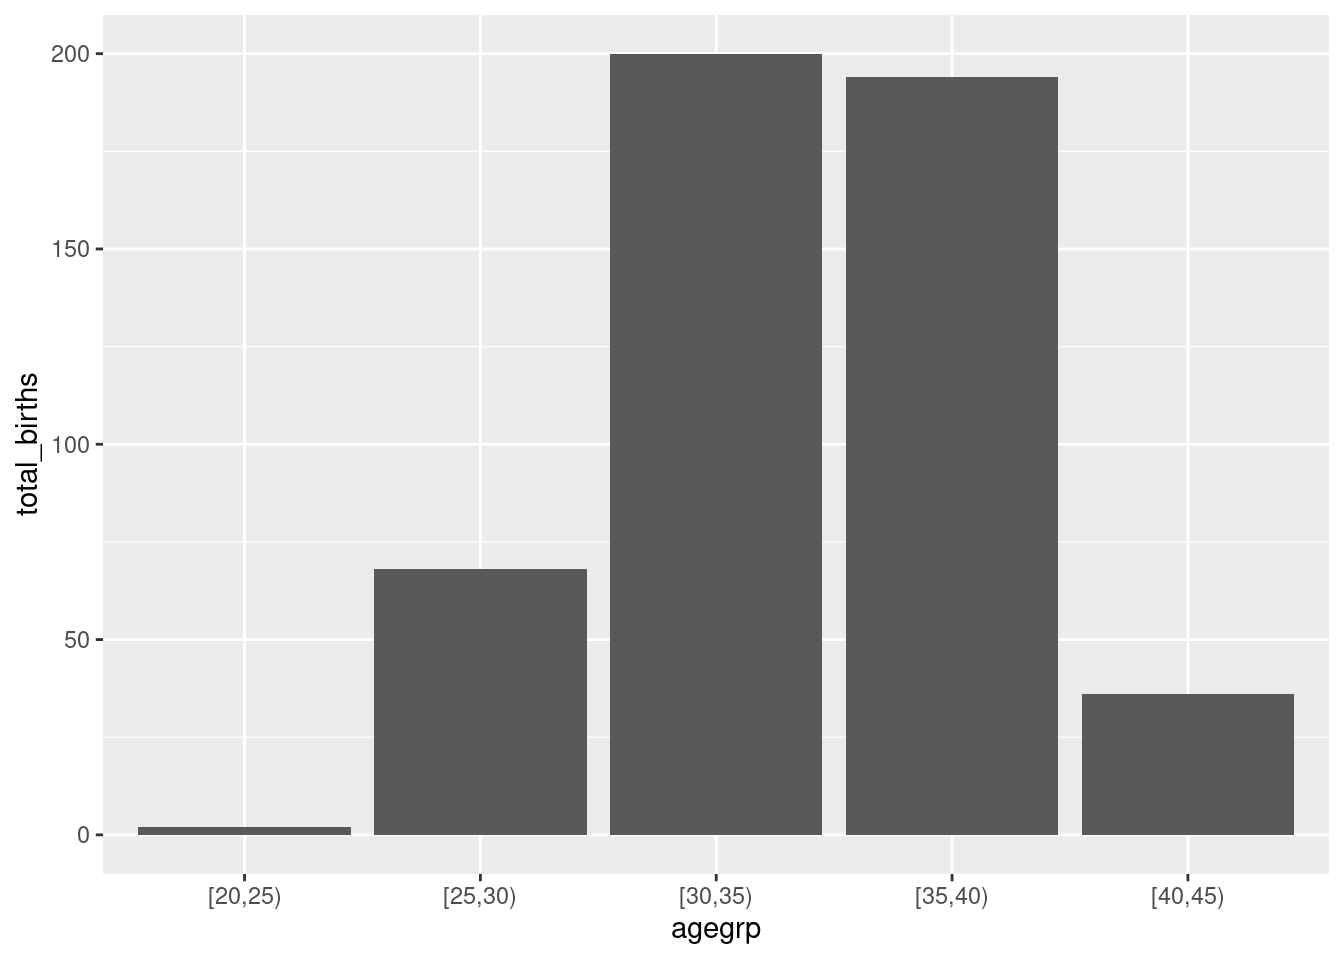
\includegraphics{tidyverse-s_files/figure-latex/unnamed-chunk-30-1.pdf}
This graph can be customize adding labels and title to the plot:

\begin{Shaded}
\begin{Highlighting}[]
\NormalTok{(gg}\FloatTok{.02} \OtherTok{\textless{}{-}}
\NormalTok{  gg}\FloatTok{.01} \SpecialCharTok{+}
  \FunctionTok{xlab}\NormalTok{(}\StringTok{"Women Age Group"}\NormalTok{) }\SpecialCharTok{+}
  \FunctionTok{ylab}\NormalTok{(}\StringTok{"Total Births"}\NormalTok{) }\SpecialCharTok{+}
  \FunctionTok{ggtitle}\NormalTok{(}\StringTok{"Number of Births per Women Age Group"}\NormalTok{))}
\end{Highlighting}
\end{Shaded}

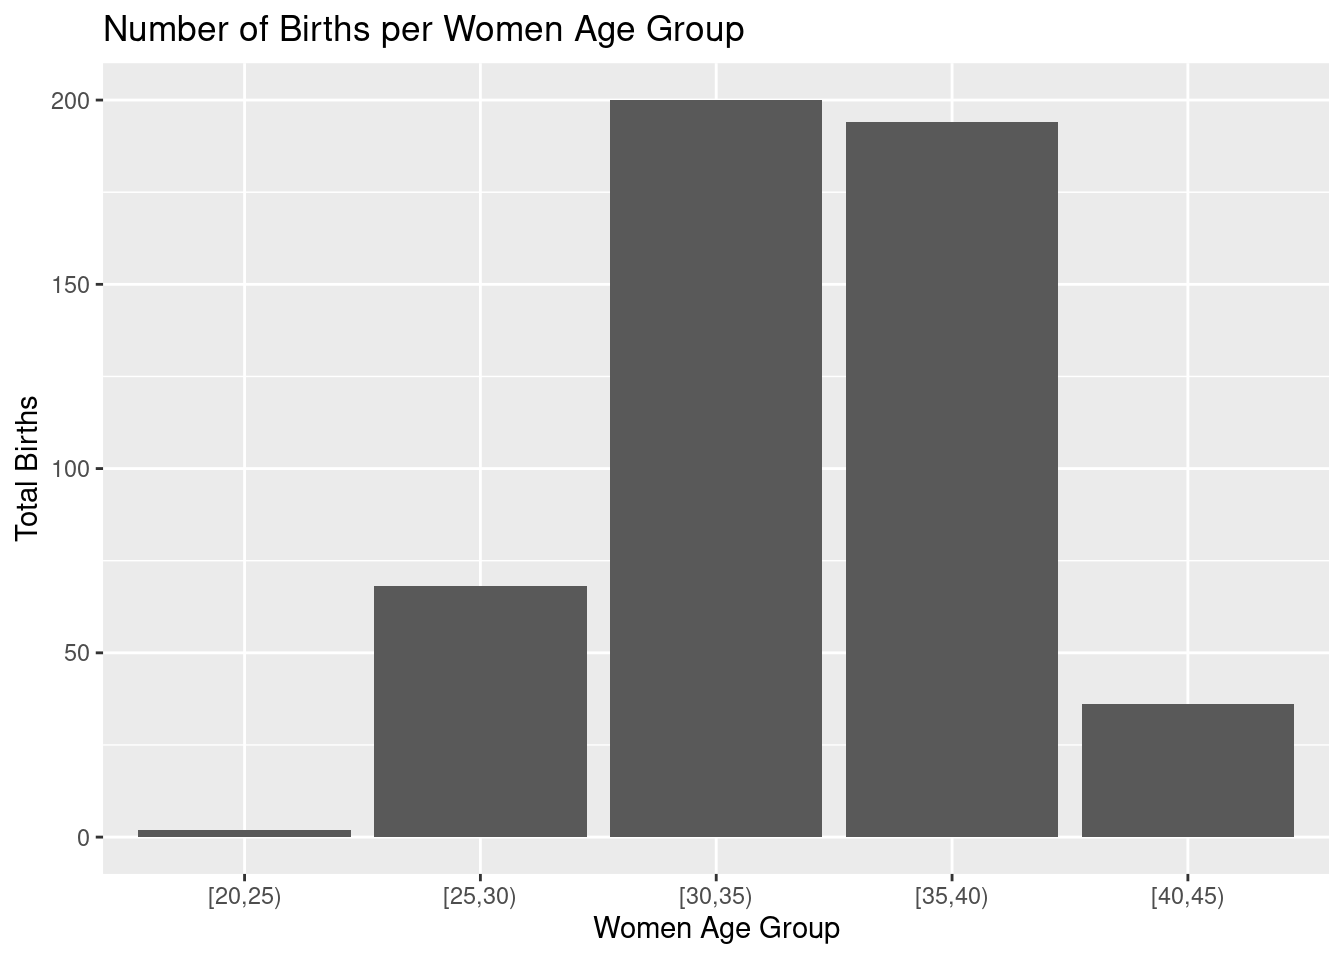
\includegraphics{tidyverse-s_files/figure-latex/unnamed-chunk-31-1.pdf}
As you can see, plots from \texttt{ggplot} family are built incrementally using the \texttt{+} operator for each additional element.

\section{pivoting data with tidyr}\label{pivoting-data-with-tidyr}

\texttt{dplyr} often comes with its good friend \texttt{tidyr} when we are performing data manipulation. \texttt{tidyr} main features is to reshape tables from long to wide format and vis-versa. Let's have an example.
Let's transform in wide format the previously created \texttt{birth\_per\_ageg} table.
We want to have a table with one column per age group containing the \texttt{total\_births} numbers.

\begin{Shaded}
\begin{Highlighting}[]
\NormalTok{birth\_per\_ageg}
\end{Highlighting}
\end{Shaded}

\begin{verbatim}
## # A tibble: 5 x 2
##   agegrp  total_births
##   <fct>          <int>
## 1 [20,25)            2
## 2 [25,30)           68
## 3 [30,35)          200
## 4 [35,40)          194
## 5 [40,45)           36
\end{verbatim}

\begin{Shaded}
\begin{Highlighting}[]
\NormalTok{birth\_per\_ageg\_wide }\OtherTok{\textless{}{-}}
\NormalTok{  birth\_per\_ageg }\SpecialCharTok{|\textgreater{}}
  \FunctionTok{pivot\_wider}\NormalTok{(}
    \AttributeTok{names\_from =} \StringTok{"agegrp"}\NormalTok{, }
    \AttributeTok{values\_from =} \StringTok{"total\_births"}
\NormalTok{  )}

\NormalTok{birth\_per\_ageg\_wide}
\end{Highlighting}
\end{Shaded}

\begin{verbatim}
## # A tibble: 1 x 5
##   `[20,25)` `[25,30)` `[30,35)` `[35,40)` `[40,45)`
##       <int>     <int>     <int>     <int>     <int>
## 1         2        68       200       194        36
\end{verbatim}

This table can easily be formatted back in long format using \texttt{pivot\_longer} function:

\begin{Shaded}
\begin{Highlighting}[]
\NormalTok{birth\_per\_ageg\_long }\OtherTok{\textless{}{-}}
\NormalTok{  birth\_per\_ageg\_wide }\SpecialCharTok{|\textgreater{}}
  \FunctionTok{pivot\_longer}\NormalTok{(}
    \AttributeTok{cols =} \DecValTok{1}\SpecialCharTok{:}\DecValTok{5}\NormalTok{, }
    \AttributeTok{names\_to =} \StringTok{"agegrp"}\NormalTok{, }
    \AttributeTok{values\_to =} \StringTok{"total\_births"}
\NormalTok{  )}

\NormalTok{birth\_per\_ageg\_long}
\end{Highlighting}
\end{Shaded}

\begin{verbatim}
## # A tibble: 5 x 2
##   agegrp  total_births
##   <chr>          <int>
## 1 [20,25)            2
## 2 [25,30)           68
## 3 [30,35)          200
## 4 [35,40)          194
## 5 [40,45)           36
\end{verbatim}

Are the tables \texttt{birth\_per\_ageg} and \texttt{birth\_per\_ageg\_long} identical?

\begin{Shaded}
\begin{Highlighting}[]
\FunctionTok{identical}\NormalTok{(birth\_per\_ageg, birth\_per\_ageg\_long)}
\end{Highlighting}
\end{Shaded}

\begin{verbatim}
## [1] FALSE
\end{verbatim}

Not really because the factor type of \texttt{agegrp} column has been lost during the transformation.
Let's convert \texttt{agegrp} column into a factor. Is the new table identical to \texttt{birth\_per\_ageg} ?

\begin{Shaded}
\begin{Highlighting}[]
\NormalTok{birth\_per\_ageg\_long\_02 }\OtherTok{\textless{}{-}}
\NormalTok{  birth\_per\_ageg\_long }\SpecialCharTok{|\textgreater{}}
  \FunctionTok{mutate}\NormalTok{(}\AttributeTok{agegrp =} \FunctionTok{as.factor}\NormalTok{(agegrp))}

\FunctionTok{identical}\NormalTok{(birth\_per\_ageg, birth\_per\_ageg\_long\_02)}
\end{Highlighting}
\end{Shaded}

\begin{verbatim}
## [1] TRUE
\end{verbatim}

Here we have seen the simplest example you can have of table reshaping with \texttt{tidyr}. If you are interested check the dedicated vignette (\texttt{vignette("pivot")}) to learn how to perform more advanced tables reshaping.

\section{reading files with readr}\label{reading-files-with-readr}

Another package from \texttt{tidyverse} that can be introduced here is \texttt{readr} that contains a set of functions equivalent to the core \texttt{R} data.frame reading functions (e.g.~\texttt{read.table()}, \texttt{read.csv()}, \texttt{read.delim()}, \ldots). The main change is that data are loaded in \texttt{R} as \texttt{tibble} instead of \texttt{data.frame}, type of variables (columns) are \emph{guessed} if possible, and some extra data checking tests are performed.

Let's explore this differences with \texttt{fem} dataset available in \texttt{data} directory.

\begin{Shaded}
\begin{Highlighting}[]
\CommentTok{\# read a csv using core R}
\NormalTok{fem.csv.core }\OtherTok{\textless{}{-}} \FunctionTok{read.csv}\NormalTok{(}\StringTok{"data/fem.csv"}\NormalTok{)}
\CommentTok{\# read a csv using tidyverse}
\NormalTok{fem.csv.tidy }\OtherTok{\textless{}{-}} \FunctionTok{read\_csv}\NormalTok{(}\StringTok{"data/fem.csv"}\NormalTok{)}
\end{Highlighting}
\end{Shaded}

\begin{verbatim}
## Rows: 118 Columns: 9
## -- Column specification --------------------------------------------------------
## Delimiter: ","
## dbl (9): ID, AGE, IQ, ANXIETY, DEPRESS, SLEEP, SEX, LIFE, WEIGHT
## 
## i Use `spec()` to retrieve the full column specification for this data.
## i Specify the column types or set `show_col_types = FALSE` to quiet this message.
\end{verbatim}

\begin{Shaded}
\begin{Highlighting}[]
\CommentTok{\# compare}
\NormalTok{fem.csv.core}
\end{Highlighting}
\end{Shaded}

\begin{verbatim}
##      ID AGE  IQ ANXIETY DEPRESS SLEEP SEX LIFE WEIGHT
## 1     1  39  94       2       2     2   1    1   2.23
## 2     2  41  89       2       2     2   1    1   1.00
## 3     3  42  83       3       3     2   1    1   1.82
## 4     4  30  99       2       2     2   1    1  -1.18
## 5     5  35  94       2       1     1   1    2  -0.14
## 6     6  44  90      NA       1     2   2    2   0.41
## 7     7  31  94       2       2    NA   1    1  -0.68
## 8     8  39  87       3       2     2   1    2   1.59
## 9     9  35  NA       3       2     2   1    1  -0.55
## 10   10  33  92       2       2     2   1    1   0.36
## 11   11  38  92       2       1     1   2    2  -0.86
## 12   12  31  94       2       2     2  NA    2   2.50
## 13   13  40  91       3       2     2   1    2   1.23
## 14   14  44  86       2       2     2   1    1   2.00
## 15   15  43  90       3       2     2   1    1   1.45
## 16   16  32  NA       1       1     1   1    2  -0.68
## 17   17  32  91       1       2     2  NA    2  -0.86
## 18   18  43  82       4       3     2   1    1   3.77
## 19   19  46  86       3       2     2   1    1   1.64
## 20   20  30  88       2       2     2   1    2   0.64
## 21   21  34  97       3       3    NA   1    1     NA
## 22   22  37  96       3       2     2   1    2     NA
## 23   23  35  95       2       1     2   1    2  -0.45
## 24   24  45  87       2       2     2   1    1   2.95
## 25   25  35 103       2       2     2   1    2  -0.95
## 26   26  31  NA       2       2     2   1    2  -0.18
## 27   27  32  91       2       2     2   1    2  -0.86
## 28   28  44  87       2       2     2   1    1   1.68
## 29   29  40  91       3       3     2   1    1   2.05
## 30   30  42  89       3       3     2   1    1   1.91
## 31   31  36  92       3      NA     2   1    1     NA
## 32   32  42  84       3       3     2   1    1   0.77
## 33   33  46  94       2      NA     2   1    1   2.18
## 34   34  41  92       2       1     2   1    2   0.77
## 35   35  30  96      NA       2     2   1    1  -1.36
## 36   36  39  96       2       2     2   2    2   0.36
## 37   37  40  86       2       3     2   1    1   0.68
## 38   38  42  92       3       2     2   1    2   0.59
## 39   39  35 102       2       2     2   1    1   1.36
## 40   40  31  82       2       2     2   1    2   0.45
## 41   41  33  92       3       3     2   1    1   0.68
## 42   42  43  90      NA      NA     2   1    1   1.55
## 43   43  37  92       2       1     1   2    2     NA
## 44   44  32  88       4       2     2   1    2     NA
## 45   45  34  98       2       2     2   1   NA   0.27
## 46   46  34  93       3       2     2   1    1   0.27
## 47   47  42  90       2       1     1   1    2   1.50
## 48   48  41  91       2       1     1   2    2   2.18
## 49   49  31  NA       3       1     2   1    2  -1.00
## 50   50  32  92       3       2     2   1    1   0.45
## 51   51  29  92       2       2     2   2    1  -0.55
## 52   52  41  91       2       2     2   1    1   1.82
## 53   53  39  91       2       2     2   1    1   2.68
## 54   54  41  86       2       1     1   1    2   0.09
## 55   55  34  95       2       1     1   1    2   1.59
## 56   56  39  91       1       1     2   2    2   1.32
## 57   57  35  96       3       2     2   2    2  -0.27
## 58   58  31 100       2       2     2   1    1  -0.27
## 59   59  32  99       4       3     2   1    1  -1.14
## 60   60  41  89       2       1     2   2    2   1.45
## 61   61  41  89       3       2     2   1    1   0.95
## 62   62  44  98       3       2     2   1    1   1.73
## 63   63  35  98       2       2     2   1    2  -1.09
## 64   64  41 103       2       2     2   1    1  -0.36
## 65   65  41  91       3       1     2   1    2   2.64
## 66   66  42  91       4       3    NA  NA    1   1.14
## 67   67  33  94       2       2     2   1    2  -0.82
## 68   68  41  91       2       1     2   1    2   1.95
## 69   69  43  85       2       2     2   2    2     NA
## 70   70  37  92       1       1     2   1    2   0.45
## 71   71  36  96       3       3     2   1    1   1.59
## 72   72  44  90       2      NA     2   1    1   1.50
## 73   73  42  87       2       2     2   2    1  -0.32
## 74   74  31  95       2       3     2   1    1  -0.73
## 75   75  29  95       3       3     2   1    1  -0.09
## 76   76  32  87       1       1     2   1    2  -1.68
## 77   77  35  95       2       2     2   1    1   1.73
## 78   78  42  88       1       1     1   1    2  -0.45
## 79   79  32  94       2       2     2   1    2   2.14
## 80   80  39  NA       3       2     2   1    1  -2.23
## 81   81  34  NA       3      NA     2   1    2     NA
## 82   82  34  87       3       3     2   1    2   1.00
## 83   83  42  92       1       1     2   2    2   2.27
## 84   84  43  86       2       3     2   1    1   0.18
## 85   85  31  93      NA       2     2   1    1  -1.91
## 86   86  31  92       2       2     2   1    2  -0.50
## 87   87  36 106       2       2     2   2    1  -0.45
## 88   88  37  93       2       2     2   1    1   1.91
## 89   89  43  95       2       2     2   1    2   1.09
## 90   90  32  95       3       2     2   1    1   2.23
## 91   91  32  92      NA      NA    NA   1    1   1.36
## 92   92  32  98       2       2     2   1    1  -0.14
## 93   93  43  92       2       2     2   1    1   0.55
## 94   94  41  88       2       2     2   1    2   1.18
## 95   95  43  85       1       1     2   1    2   0.86
## 96   96  39  92       2       2     2   1    2   1.59
## 97   97  41  84       2       2     2   1    1  -0.27
## 98   98  41  92       2       1     2   1    2   0.64
## 99   99  32  91       2       2     2   1    1   2.59
## 100 100  44  86       3       2     2   1    1   2.09
## 101 101  42  92       3       2     2   1    2     NA
## 102 102  39  89       2       2     2   1    2   0.91
## 103 103  45  NA       2       2     2   1    1   0.27
## 104 104  39  96       3      NA     2   1    1     NA
## 105 105  31  97       2      NA    NA  NA    1   1.27
## 106 106  34  92       3       2     2   1    1  -0.95
## 107 107  41  92       2       2     2   1    1  -1.14
## 108 108  33  98       3       2     2   1    1   1.14
## 109 109  34  91       2       1     1   1    2   2.59
## 110 100  42  91       3       3     2   1    1   1.09
## 111 111  40  89       3       1     1   2    2   0.68
## 112 112  35  94       3       3     2   1    1   0.77
## 113 113  41  90       3       2     2   1    1   1.14
## 114 114  32  96       2       1     1   1    2     NA
## 115 115  39  87       2       2     2   2    1     NA
## 116 116  41  86       3       2     1   2    1  -0.45
## 117 117  33  89       1       1     1   2    2   2.95
## 118 118  42  NA       3       2     2   1    1   2.23
\end{verbatim}

\begin{Shaded}
\begin{Highlighting}[]
\NormalTok{fem.csv.tidy}
\end{Highlighting}
\end{Shaded}

\begin{verbatim}
## # A tibble: 118 x 9
##       ID   AGE    IQ ANXIETY DEPRESS SLEEP   SEX  LIFE WEIGHT
##    <dbl> <dbl> <dbl>   <dbl>   <dbl> <dbl> <dbl> <dbl>  <dbl>
##  1     1    39    94       2       2     2     1     1   2.23
##  2     2    41    89       2       2     2     1     1   1   
##  3     3    42    83       3       3     2     1     1   1.82
##  4     4    30    99       2       2     2     1     1  -1.18
##  5     5    35    94       2       1     1     1     2  -0.14
##  6     6    44    90      NA       1     2     2     2   0.41
##  7     7    31    94       2       2    NA     1     1  -0.68
##  8     8    39    87       3       2     2     1     2   1.59
##  9     9    35    NA       3       2     2     1     1  -0.55
## 10    10    33    92       2       2     2     1     1   0.36
## # i 108 more rows
\end{verbatim}

\begin{Shaded}
\begin{Highlighting}[]
\CommentTok{\# table dimensions}
\FunctionTok{dim}\NormalTok{(fem.csv.core)}
\end{Highlighting}
\end{Shaded}

\begin{verbatim}
## [1] 118   9
\end{verbatim}

\begin{Shaded}
\begin{Highlighting}[]
\FunctionTok{dim}\NormalTok{(fem.csv.tidy)}
\end{Highlighting}
\end{Shaded}

\begin{verbatim}
## [1] 118   9
\end{verbatim}

\begin{Shaded}
\begin{Highlighting}[]
\CommentTok{\# compare column types}
\FunctionTok{map}\NormalTok{(fem.csv.core, class)}
\end{Highlighting}
\end{Shaded}

\begin{verbatim}
## $ID
## [1] "integer"
## 
## $AGE
## [1] "integer"
## 
## $IQ
## [1] "integer"
## 
## $ANXIETY
## [1] "integer"
## 
## $DEPRESS
## [1] "integer"
## 
## $SLEEP
## [1] "integer"
## 
## $SEX
## [1] "integer"
## 
## $LIFE
## [1] "integer"
## 
## $WEIGHT
## [1] "numeric"
\end{verbatim}

\begin{Shaded}
\begin{Highlighting}[]
\FunctionTok{map}\NormalTok{(fem.csv.tidy, class)}
\end{Highlighting}
\end{Shaded}

\begin{verbatim}
## $ID
## [1] "numeric"
## 
## $AGE
## [1] "numeric"
## 
## $IQ
## [1] "numeric"
## 
## $ANXIETY
## [1] "numeric"
## 
## $DEPRESS
## [1] "numeric"
## 
## $SLEEP
## [1] "numeric"
## 
## $SEX
## [1] "numeric"
## 
## $LIFE
## [1] "numeric"
## 
## $WEIGHT
## [1] "numeric"
\end{verbatim}

\textbf{note:} in case you do not fully get the last lines and the \texttt{map()} call, it will be explained in the next section on \texttt{purrr} package.

Here we see that the only difference is the type of object loaded \texttt{data.frame} vs \texttt{tibble} and the default type chosen to cast numeric values (\texttt{integer} vs \texttt{numeric}).

What about loading \texttt{occoh.txt} you will be using in some other practical in the coming days.

\begin{Shaded}
\begin{Highlighting}[]
\CommentTok{\# read a csv using core R}
\NormalTok{occoh.txt.core }\OtherTok{\textless{}{-}} \FunctionTok{read.table}\NormalTok{(}\StringTok{"data/occoh.txt"}\NormalTok{)}
\CommentTok{\# read a csv using tidyverse}
\NormalTok{occoh.txt.tidy }\OtherTok{\textless{}{-}} \FunctionTok{read\_table}\NormalTok{(}\StringTok{"data/occoh.txt"}\NormalTok{)}
\end{Highlighting}
\end{Shaded}

\begin{verbatim}
## 
## -- Column specification --------------------------------------------------------
## cols(
##   id = col_double(),
##   birth = col_double(),
##   entry = col_date(format = ""),
##   exit = col_date(format = ""),
##   death = col_date(format = ""),
##   chdeath = col_double()
## )
\end{verbatim}

\begin{verbatim}
## Warning: 1501 parsing failures.
## row col  expected    actual             file
##   1  -- 6 columns 7 columns 'data/occoh.txt'
##   2  -- 6 columns 7 columns 'data/occoh.txt'
##   3  -- 6 columns 7 columns 'data/occoh.txt'
##   4  -- 6 columns 7 columns 'data/occoh.txt'
##   5  -- 6 columns 7 columns 'data/occoh.txt'
## ... ... ......... ......... ................
## See problems(...) for more details.
\end{verbatim}

\begin{Shaded}
\begin{Highlighting}[]
\NormalTok{occoh.txt.tidy }\OtherTok{\textless{}{-}} \FunctionTok{read\_table}\NormalTok{(}\StringTok{"data/occoh.txt"}\NormalTok{)}
\end{Highlighting}
\end{Shaded}

\begin{verbatim}
## 
## -- Column specification --------------------------------------------------------
## cols(
##   id = col_double(),
##   birth = col_double(),
##   entry = col_date(format = ""),
##   exit = col_date(format = ""),
##   death = col_date(format = ""),
##   chdeath = col_double()
## )
\end{verbatim}

\begin{verbatim}
## Warning: 1501 parsing failures.
## row col  expected    actual             file
##   1  -- 6 columns 7 columns 'data/occoh.txt'
##   2  -- 6 columns 7 columns 'data/occoh.txt'
##   3  -- 6 columns 7 columns 'data/occoh.txt'
##   4  -- 6 columns 7 columns 'data/occoh.txt'
##   5  -- 6 columns 7 columns 'data/occoh.txt'
## ... ... ......... ......... ................
## See problems(...) for more details.
\end{verbatim}

\begin{Shaded}
\begin{Highlighting}[]
\CommentTok{\# compare}
\NormalTok{occoh.txt.core}
\end{Highlighting}
\end{Shaded}

\begin{verbatim}
##        id      birth      entry       exit death chdeath
## 1       1 1943-02-19 1990-08-14 2009-12-31     0       0
## 2       2 1934-07-06 1990-08-14 2009-12-31     0       0
## 3       3 1939-03-05 1990-08-14 2009-12-31     0       0
## 4       4 1939-07-03 1990-08-14 2009-12-31     0       0
## 5       5 1935-02-18 1990-08-14 2006-03-13     1       0
## 6       6 1936-03-07 1990-08-14 2007-06-10     1       0
## 7       7 1944-03-30 1990-08-15 2007-04-14     1       0
## 8       8 1942-11-24 1990-08-15 2006-10-30     1       1
## 9       9 1942-09-11 1990-08-15 2009-12-31     0       0
## 10     10 1931-03-01 1990-08-15 2009-12-31     0       0
## 11     11 1943-02-20 1990-08-15 2009-12-31     0       0
## 12     12 1934-07-26 1990-08-15 2009-12-31     0       0
## 13     13 1935-10-04 1990-08-18 2009-12-31     0       0
## 14     14 1931-12-09 1990-08-18 2009-12-31     0       0
## 15     15 1931-08-24 1990-08-18 2009-12-31     0       0
## 17     16 1947-03-29 1990-08-18 2009-12-31     0       0
## 18     17 1939-03-19 1990-08-18 2009-12-31     0       0
## 19     18 1940-07-19 1990-08-18 2009-12-31     0       0
## 20     19 1945-08-10 1990-08-18 2005-07-30     1       0
## 21     20 1945-01-13 1990-08-18 2009-12-31     0       0
## 22     21 1942-02-08 1990-08-18 2009-12-31     0       0
## 23     22 1941-04-11 1990-08-18 2009-12-31     0       0
## 24     23 1948-07-07 1990-08-18 2009-12-31     0       0
## 25     24 1944-02-12 1990-08-18 2009-12-31     0       0
## 26     25 1947-11-19 1990-08-19 2009-12-31     0       0
## 27     26 1945-11-24 1990-08-19 2009-12-31     0       0
## 28     27 1941-05-01 1990-08-19 2009-12-31     0       0
## 29     28 1932-03-19 1990-08-19 2009-12-31     0       0
## 30     29 1944-02-20 1990-08-19 2009-12-31     0       0
## 31     30 1943-09-26 1990-08-19 2009-12-31     0       0
## 32     31 1948-08-29 1990-08-20 2009-12-31     0       0
## 33     32 1949-06-18 1990-08-20 2009-12-31     0       0
## 34     33 1937-08-15 1990-08-20 2009-12-31     0       0
## 35     34 1938-09-14 1990-08-20 2009-12-31     0       0
## 36     35 1943-11-13 1990-08-20 2009-12-31     0       0
## 37     36 1949-01-22 1990-08-20 2009-12-31     0       0
## 38     37 1950-04-30 1990-08-21 2009-12-31     0       0
## 39     38 1943-09-09 1990-08-21 2009-12-31     0       0
## 40     39 1943-11-25 1990-08-21 2009-12-31     0       0
## 41     40 1945-06-22 1990-08-21 1995-03-26     1       0
## 42     41 1950-06-11 1990-08-21 2009-12-14     1       1
## 43     42 1933-10-06 1990-08-21 2004-01-14     1       1
## 44     43 1936-04-28 1990-08-21 2003-06-13     1       1
## 45     44 1943-06-29 1990-08-22 2009-12-31     0       0
## 46     45 1945-06-18 1990-08-22 2009-12-31     0       0
## 47     46 1942-01-05 1990-08-22 2009-12-31     0       0
## 48     47 1930-03-01 1990-08-22 2009-12-31     0       0
## 49     48 1932-01-10 1990-08-22 2005-12-08     1       0
## 50     49 1939-01-31 1990-08-22 2009-12-31     0       0
## 51     50 1947-03-10 1990-08-25 2009-12-31     0       0
## 52     51 1935-04-08 1990-08-26 2006-04-26     1       1
## 54     52 1950-05-10 1990-08-27 2009-12-31     0       0
## 55     53 1939-02-14 1990-08-27 2009-12-31     0       0
## 56     54 1943-10-20 1990-08-27 2009-12-31     0       0
## 57     55 1935-08-21 1990-08-27 2009-12-31     0       0
## 59     56 1935-07-21 1990-08-29 2009-12-31     0       0
## 60     57 1942-01-01 1990-08-29 2009-12-31     0       0
## 61     58 1944-05-29 1990-09-05 2009-12-31     0       0
## 62     59 1936-08-17 1990-09-05 2009-12-31     0       0
## 63     60 1945-01-20 1990-09-12 2009-12-31     0       0
## 64     61 1944-01-14 1990-09-12 2009-12-31     0       0
## 65     62 1932-09-19 1990-09-29 1999-02-01     1       1
## 66     63 1941-02-28 1990-09-29 2004-06-06     1       1
## 67     64 1944-09-21 1990-09-29 2009-12-31     0       0
## 68     65 1940-07-04 1990-09-29 2009-12-31     0       0
## 69     66 1945-04-23 1990-09-29 2006-09-15     1       0
## 70     67 1944-08-21 1990-09-29 2009-12-31     0       0
## 71     68 1937-02-06 1990-09-29 2009-12-19     1       0
## 72     69 1948-04-28 1990-09-29 2009-12-31     0       0
## 73     70 1937-06-11 1990-09-29 2009-12-31     0       0
## 74     71 1948-06-28 1990-09-30 2009-12-31     0       0
## 75     72 1945-07-22 1990-09-30 2009-12-31     0       0
## 76     73 1939-08-14 1990-09-30 2009-12-31     0       0
## 77     74 1946-05-02 1990-09-30 2009-12-31     0       0
## 78     75 1931-09-05 1990-09-30 2000-01-27     1       0
## 79     76 1943-07-03 1990-09-30 2009-12-31     0       0
## 80     77 1938-06-29 1990-10-01 2009-12-31     0       0
## 81     78 1936-06-27 1990-10-01 2009-12-31     0       0
## 82     79 1944-11-11 1990-10-01 2009-12-31     0       0
## 83     80 1944-05-22 1990-10-01 2009-12-31     0       0
## 84     81 1947-06-07 1990-10-01 2009-12-31     0       0
## 85     82 1943-09-12 1990-10-01 2009-12-31     0       0
## 86     83 1933-10-14 1990-10-01 2009-12-31     0       0
## 87     84 1943-01-23 1990-10-01 2009-12-31     0       0
## 88     85 1945-07-12 1990-10-01 2008-02-09     1       1
## 89     86 1947-10-15 1990-10-02 2009-12-31     0       0
## 90     87 1935-12-23 1990-10-02 2009-12-31     0       0
## 91     88 1931-09-09 1990-10-02 2009-12-31     0       0
## 92     89 1938-11-18 1990-10-03 2009-12-31     0       0
## 93     90 1943-04-10 1990-10-03 2009-12-31     0       0
## 94     91 1930-06-26 1990-10-03 2009-12-31     0       0
## 95     92 1941-12-15 1990-10-03 2009-12-31     0       0
## 96     93 1947-07-29 1990-10-03 2009-12-31     0       0
## 97     94 1948-10-30 1990-10-03 2009-12-31     0       0
## 98     95 1943-03-19 1990-10-03 2009-11-21     1       1
## 99     96 1945-09-13 1990-10-06 2009-12-31     0       0
## 100    97 1933-01-29 1990-10-06 1993-11-28     1       1
## 101    98 1935-05-07 1990-10-06 2004-12-11     1       0
## 102    99 1940-07-18 1990-10-06 1997-08-19     1       0
## 104   100 1946-01-16 1990-10-06 2009-12-31     0       0
## 105   101 1940-02-12 1990-10-06 2004-08-02     1       0
## 106   102 1950-05-13 1990-10-07 2009-12-31     0       0
## 107   103 1937-04-11 1990-10-07 2000-01-15     1       1
## 108   104 1936-08-28 1990-10-07 2001-04-12     1       1
## 109   105 1935-12-04 1990-10-07 2009-12-31     0       0
## 110   106 1943-03-06 1990-10-07 2009-12-31     0       0
## 111   107 1950-08-30 1990-10-07 2009-12-31     0       0
## 112   108 1942-04-16 1990-10-08 2009-12-31     0       0
## 113   109 1941-04-16 1990-10-08 2009-12-31     0       0
## 114   110 1946-02-18 1990-10-08 2009-12-31     0       0
## 115   111 1946-01-28 1990-10-08 2009-12-31     0       0
## 116   112 1938-08-28 1990-10-08 2009-12-31     0       0
## 117   113 1934-01-08 1990-10-09 2009-12-31     0       0
## 118   114 1935-02-04 1990-10-09 2009-12-31     0       0
## 119   115 1943-01-06 1990-10-09 2007-12-19     1       1
## 120   116 1943-07-27 1990-10-09 2009-12-31     0       0
## 121   117 1933-02-07 1990-10-09 2009-12-31     0       0
## 122   118 1934-04-28 1990-10-09 2009-06-29     1       0
## 123   119 1938-12-11 1990-10-09 2009-12-31     0       0
## 124   120 1931-06-21 1990-10-09 1993-05-12     1       1
## 125   121 1949-09-12 1990-10-10 2009-12-31     0       0
## 126   122 1949-01-27 1990-10-10 2009-12-31     0       0
## 127   123 1947-01-22 1990-10-10 2009-12-31     0       0
## 128   124 1929-12-23 1990-10-10 1993-02-03     1       0
## 129   125 1931-02-19 1990-10-15 2006-06-08     1       0
## 130   126 1938-02-24 1990-10-15 2009-12-31     0       0
## 131   127 1942-10-26 1990-10-15 2009-12-31     0       0
## 132   128 1940-10-14 1990-10-15 2009-12-31     0       0
## 133   129 1934-12-28 1990-10-15 2009-12-31     0       0
## 134   130 1945-02-23 1990-10-27 2009-12-31     0       0
## 135   131 1932-05-12 1990-10-27 2009-12-31     0       0
## 136   132 1942-07-25 1990-10-27 2009-12-31     0       0
## 137   133 1933-06-25 1990-10-28 1996-12-15     1       0
## 138   134 1937-12-05 1990-10-28 2009-12-31     0       0
## 139   135 1947-06-23 1990-10-28 2009-12-31     0       0
## 140   136 1945-09-04 1990-10-29 1999-05-23     1       1
## 142   137 1931-08-29 1990-10-29 2002-06-01     1       0
## 143   138 1930-02-11 1990-10-29 2009-12-31     0       0
## 144   139 1944-05-12 1990-10-29 2009-12-31     0       0
## 146   140 1936-07-01 1990-10-29 2009-12-31     0       0
## 147   141 1937-10-10 1990-10-30 2009-12-31     0       0
## 148   142 1945-01-25 1990-10-30 2009-12-31     0       0
## 149   143 1939-06-11 1990-10-30 2009-12-31     0       0
## 150   144 1941-06-15 1990-10-30 2009-12-31     0       0
## 151   145 1941-08-01 1990-10-30 2009-12-31     0       0
## 152   146 1938-09-15 1990-10-30 2009-12-31     0       0
## 153   147 1939-11-30 1990-10-30 2009-12-31     0       0
## 154   148 1936-11-27 1990-10-30 1992-07-05     1       1
## 155   149 1935-04-05 1990-10-30 1992-04-06     1       1
## 156   150 1943-03-08 1990-10-31 2009-12-31     0       0
## 160   151 1942-03-03 1990-10-31 2009-12-31     0       0
## 161   152 1937-03-12 1990-11-03 2009-12-31     0       0
## 162   153 1941-07-27 1990-11-03 2009-12-31     0       0
## 163   154 1940-01-23 1990-11-03 2006-06-01     1       1
## 164   155 1936-02-24 1990-11-03 2000-01-23     1       0
## 165   156 1949-08-08 1990-11-03 2009-12-31     0       0
## 167   157 1936-01-13 1990-11-04 2009-12-31     0       0
## 168   158 1949-05-16 1990-11-04 2009-12-31     0       0
## 169   159 1939-08-06 1990-11-04 2009-12-31     0       0
## 170   160 1948-06-04 1990-11-04 2009-12-31     0       0
## 173   161 1948-12-14 1990-11-04 2009-12-31     0       0
## 174   162 1946-05-02 1990-11-04 2009-12-31     0       0
## 175   163 1931-05-16 1990-11-05 2009-12-31     0       0
## 176   164 1942-09-16 1990-11-05 2009-12-31     0       0
## 177   165 1937-09-16 1990-11-05 2009-12-31     0       0
## 178   166 1950-06-14 1990-11-05 2009-12-31     0       0
## 180   167 1950-10-17 1990-11-05 2009-12-31     0       0
## 181   168 1936-11-17 1990-11-05 2000-06-19     1       1
## 182   169 1942-05-15 1990-11-05 2009-12-31     0       0
## 183   170 1943-01-18 1990-11-06 2002-06-20     1       0
## 184   171 1938-09-10 1990-11-06 2009-12-31     0       0
## 185   172 1948-05-20 1990-11-06 2009-12-31     0       0
## 186   173 1944-07-30 1990-11-06 2009-12-31     0       0
## 187   174 1938-10-06 1990-11-06 2009-12-31     0       0
## 188   175 1944-07-11 1990-11-06 2009-12-31     0       0
## 189   176 1944-03-31 1990-11-06 2009-12-31     0       0
## 190   177 1944-08-21 1990-11-07 2009-12-31     0       0
## 191   178 1940-11-12 1990-11-07 2009-12-31     0       0
## 192   179 1939-01-24 1990-11-07 2009-10-05     1       0
## 193   180 1932-01-04 1990-11-07 2009-12-31     0       0
## 194   181 1935-01-12 1990-11-07 2009-12-31     0       0
## 195   182 1949-05-10 1990-11-07 2009-12-31     0       0
## 196   183 1946-06-17 1990-11-07 2009-12-31     0       0
## 197   184 1943-12-27 1990-11-07 1997-12-14     1       1
## 198   185 1949-09-05 1990-11-07 2009-12-31     0       0
## 199   186 1943-02-21 1990-11-07 2009-12-31     0       0
## 200   187 1939-02-20 1990-11-10 2009-12-31     0       0
## 201   188 1946-12-26 1990-11-10 2009-12-31     0       0
## 203   189 1939-01-03 1990-11-10 2009-12-31     0       0
## 204   190 1946-12-31 1990-11-10 2007-01-17     1       0
## 205   191 1942-05-09 1990-11-10 2000-07-01     1       1
## 206   192 1942-10-14 1990-11-11 2009-12-31     0       0
## 207   193 1942-05-24 1990-11-11 2009-12-31     0       0
## 208   194 1945-03-13 1990-11-11 2009-12-31     0       0
## 209   195 1929-08-01 1990-11-11 2009-12-31     0       0
## 210   196 1949-11-25 1990-11-11 2009-12-31     0       0
## 211   197 1938-04-25 1990-11-12 2009-12-31     0       0
## 212   198 1937-05-10 1990-11-12 2009-12-31     0       0
## 213   199 1936-04-29 1990-11-12 2006-11-26     1       1
## 214   200 1931-05-21 1990-11-12 1999-02-02     1       0
## 215   201 1932-02-14 1990-11-13 1996-07-24     1       1
## 216   202 1947-06-21 1990-11-13 2009-05-13     1       0
## 217   203 1942-10-31 1990-11-13 2009-12-31     0       0
## 218   204 1943-04-22 1990-11-13 2009-12-31     0       0
## 219   205 1945-01-25 1990-11-14 2009-12-31     0       0
## 220   206 1945-05-28 1990-11-14 2009-12-31     0       0
## 221   207 1931-05-13 1990-11-14 2009-12-31     0       0
## 222   208 1940-08-17 1990-11-14 2000-11-05     1       0
## 223   209 1948-03-17 1990-11-14 2002-05-27     1       0
## 225   210 1930-09-17 1990-11-17 1998-12-06     1       0
## 226   211 1949-10-03 1990-11-17 2009-12-31     0       0
## 227   212 1948-01-16 1990-11-17 2009-12-31     0       0
## 228   213 1948-04-20 1990-11-17 2009-12-31     0       0
## 229   214 1944-03-09 1990-11-17 2009-12-31     0       0
## 230   215 1933-03-21 1990-11-17 2009-12-31     0       0
## 231   216 1946-10-08 1990-11-17 2009-12-31     0       0
## 232   217 1936-04-19 1990-11-18 2009-12-31     0       0
## 233   218 1949-12-24 1990-11-18 2006-03-28     1       0
## 234   219 1934-09-24 1990-11-18 2009-12-31     0       0
## 235   220 1944-12-13 1990-11-18 2009-12-31     0       0
## 236   221 1944-02-28 1990-11-18 2009-12-31     0       0
## 237   222 1948-07-20 1990-11-18 2009-12-31     0       0
## 238   223 1941-04-28 1990-11-18 2009-12-31     0       0
## 239   224 1946-07-04 1990-11-19 2009-12-31     0       0
## 240   225 1939-04-25 1990-11-19 2009-12-31     0       0
## 241   226 1934-02-11 1990-11-19 2009-12-31     0       0
## 242   227 1943-11-21 1990-12-08 2009-12-31     0       0
## 243   228 1935-04-25 1990-12-08 2009-12-31     0       0
## 244   229 1938-01-03 1990-12-08 2009-12-31     0       0
## 245   230 1947-02-23 1990-12-08 2009-12-31     0       0
## 246   231 1943-04-06 1990-12-08 2009-12-31     0       0
## 247   232 1944-10-03 1990-12-08 2009-12-31     0       0
## 248   233 1948-06-14 1990-12-09 2009-12-31     0       0
## 249   234 1936-04-23 1990-12-09 2009-12-31     0       0
## 250   235 1933-03-31 1990-12-09 2009-12-31     0       0
## 251   236 1934-09-30 1990-12-09 2008-10-14     1       0
## 252   237 1933-03-06 1990-12-09 2005-02-18     1       0
## 253   238 1942-05-10 1990-12-09 2009-12-31     0       0
## 255   239 1933-09-08 1990-12-10 2009-12-31     0       0
## 256   240 1945-11-17 1990-12-10 2009-12-31     0       0
## 257   241 1943-09-15 1990-12-10 2009-12-31     0       0
## 258   242 1933-07-27 1990-12-10 2009-12-31     0       0
## 259   243 1942-10-05 1990-12-10 2009-12-31     0       0
## 260   244 1950-02-06 1990-12-10 2009-12-31     0       0
## 261   245 1937-03-18 1990-12-10 2009-12-31     0       0
## 262   246 1930-10-03 1990-12-29 2003-03-07     1       0
## 263   247 1941-07-07 1990-12-29 2009-12-31     0       0
## 264   248 1935-11-16 1990-12-30 2000-04-13     1       0
## 266   249 1933-03-27 1990-12-30 2009-12-31     0       0
## 267   250 1933-07-05 1990-12-30 1995-05-19     1       0
## 268   251 1945-08-18 1990-12-31 2009-12-31     0       0
## 269   252 1939-04-04 1990-12-31 2005-11-08     1       1
## 270   253 1945-01-21 1991-01-01 2009-12-31     0       0
## 271   254 1944-04-28 1991-01-01 2009-12-31     0       0
## 272   255 1934-08-30 1991-01-01 1992-02-25     1       1
## 273   256 1933-12-29 1991-01-01 2009-12-31     0       0
## 274   257 1930-09-08 1991-01-01 2006-12-15     1       1
## 275   258 1930-12-31 1991-01-02 1995-07-16     1       0
## 276   259 1941-05-18 1991-01-02 2009-12-31     0       0
## 277   260 1944-12-02 1991-01-02 2004-05-28     1       0
## 278   261 1943-06-14 1991-01-02 2009-12-31     0       0
## 279   262 1940-04-27 1991-01-02 2009-12-31     0       0
## 281   263 1938-01-10 1991-01-05 2009-12-31     0       0
## 282   264 1931-01-28 1991-01-05 2002-06-04     1       0
## 283   265 1945-10-18 1991-01-05 2009-12-31     0       0
## 285   266 1948-03-09 1991-01-05 2009-12-31     0       0
## 286   267 1944-10-18 1991-01-06 2009-12-31     0       0
## 288   268 1949-11-02 1991-01-06 2009-12-31     0       0
## 289   269 1935-03-31 1991-01-06 2009-12-31     0       0
## 290   270 1943-04-01 1991-01-06 2009-12-31     0       0
## 291   271 1930-10-24 1991-01-06 2009-12-31     0       0
## 292   272 1944-04-16 1991-01-06 2009-12-31     0       0
## 293   273 1941-06-13 1991-01-07 2009-12-31     0       0
## 294   274 1946-05-09 1991-01-07 2009-12-31     0       0
## 295   275 1933-02-28 1991-01-07 2009-12-31     0       0
## 296   276 1935-07-05 1991-01-08 2009-12-31     0       0
## 297   277 1949-12-24 1991-01-08 2009-12-31     0       0
## 298   278 1943-03-01 1991-01-08 2009-12-31     0       0
## 299   279 1930-02-24 1991-01-08 2009-12-31     0       0
## 300   280 1948-09-02 1991-01-09 2009-12-31     0       0
## 301   281 1940-04-04 1991-01-09 2009-12-31     0       0
## 302   282 1950-06-23 1991-01-09 2003-02-07     1       0
## 303   283 1942-10-16 1991-01-09 2009-12-31     0       0
## 304   284 1949-08-27 1991-01-09 2009-12-31     0       0
## 305   285 1930-07-19 1991-01-12 2003-03-06     1       0
## 306   286 1944-08-01 1991-01-12 2009-12-31     0       0
## 307   287 1942-04-19 1991-01-12 2009-12-31     0       0
## 308   288 1944-03-28 1991-01-12 2007-09-12     1       1
## 309   289 1945-01-09 1991-01-12 2009-12-31     0       0
## 310   290 1934-05-25 1991-01-12 2009-12-31     0       0
## 311   291 1939-04-19 1991-01-13 1997-05-27     1       0
## 312   292 1943-02-13 1991-01-13 2009-12-31     0       0
## 313   293 1943-01-02 1991-01-13 2009-12-31     0       0
## 314   294 1937-01-01 1991-01-13 2008-01-30     1       0
## 316   295 1935-02-18 1991-01-13 1995-04-12     1       0
## 317   296 1930-01-25 1991-01-13 1995-12-03     1       1
## 319   297 1937-12-17 1991-01-14 2009-12-31     0       0
## 320   298 1935-01-02 1991-01-14 2008-07-17     1       0
## 321   299 1946-05-19 1991-01-14 2009-12-31     0       0
## 322   300 1948-05-03 1991-01-14 2009-12-31     0       0
## 323   301 1942-09-01 1991-01-14 2009-12-31     0       0
## 324   302 1931-04-06 1991-01-14 2009-12-31     0       0
## 325   303 1945-02-20 1991-01-15 2009-12-31     0       0
## 327   304 1942-04-08 1991-01-15 2001-10-13     1       0
## 328   305 1943-03-22 1991-01-15 2009-12-31     0       0
## 329   306 1939-05-28 1991-01-15 2009-12-31     0       0
## 330   307 1934-06-20 1991-01-30 2009-12-31     0       0
## 331   308 1942-06-24 1991-01-30 2008-03-23     1       1
## 333   309 1942-02-14 1991-01-30 2009-12-31     0       0
## 334   310 1940-01-07 1991-03-30 2009-12-31     0       0
## 335   311 1945-11-18 1991-03-30 2009-12-31     0       0
## 337   312 1942-09-30 1991-03-30 1996-08-23     1       0
## 339   313 1940-02-21 1991-03-30 2009-12-31     0       0
## 340   314 1943-09-22 1991-03-30 2009-12-31     0       0
## 341   315 1945-10-05 1991-03-30 2009-12-31     0       0
## 342   316 1945-09-04 1991-03-30 2009-12-31     0       0
## 343   317 1947-04-18 1991-03-30 2009-12-31     0       0
## 344   318 1949-07-29 1991-03-30 2007-12-06     1       1
## 345   319 1941-06-16 1991-03-30 1995-12-17     1       1
## 346   320 1941-04-23 1991-03-31 2009-12-31     0       0
## 347   321 1931-03-31 1991-03-31 2009-12-31     0       0
## 348   322 1932-07-27 1991-03-31 1996-05-23     1       1
## 349   323 1935-02-05 1991-03-31 2009-12-31     0       0
## 350   324 1947-06-27 1991-03-31 2009-12-31     0       0
## 351   325 1937-12-18 1991-03-31 2009-12-31     0       0
## 352   326 1948-11-10 1991-03-31 2009-12-31     0       0
## 353   327 1944-06-11 1991-04-01 2009-12-31     0       0
## 354   328 1943-04-28 1991-04-01 2009-12-31     0       0
## 355   329 1938-03-09 1991-04-01 2009-12-31     0       0
## 356   330 1945-12-04 1991-04-01 2009-12-31     0       0
## 357   331 1942-10-21 1991-04-01 2009-12-31     0       0
## 358   332 1944-07-31 1991-04-01 2009-12-31     0       0
## 359   333 1940-03-11 1991-04-01 2009-12-31     0       0
## 360   334 1932-08-28 1991-04-01 2009-12-31     0       0
## 361   335 1933-02-16 1991-04-02 1996-05-13     1       1
## 362   336 1930-07-05 1991-04-02 1998-08-28     1       1
## 363   337 1937-01-18 1991-04-02 2009-12-31     0       0
## 364   338 1947-08-29 1991-04-03 2001-04-13     1       0
## 365   339 1938-12-17 1991-04-03 2000-03-04     1       1
## 366   340 1945-09-26 1991-04-03 2009-12-31     0       0
## 369   341 1943-05-15 1991-04-03 2009-12-31     0       0
## 370   342 1937-07-09 1991-04-06 2009-12-31     0       0
## 371   343 1939-04-16 1991-04-06 2009-12-31     0       0
## 372   344 1946-03-10 1991-04-06 2009-12-31     0       0
## 373   345 1935-07-01 1991-04-06 2009-12-31     0       0
## 374   346 1946-02-12 1991-04-07 2009-12-31     0       0
## 375   347 1950-06-09 1991-04-07 2009-12-31     0       0
## 376   348 1940-08-13 1991-04-07 2009-12-31     0       0
## 377   349 1939-11-28 1991-04-07 2009-12-31     0       0
## 378   350 1936-08-21 1991-04-07 2009-12-31     0       0
## 379   351 1943-04-16 1991-04-08 2009-12-31     0       0
## 380   352 1933-10-25 1991-04-08 2007-01-24     1       1
## 381   353 1934-06-13 1991-04-08 2009-12-31     0       0
## 382   354 1933-06-20 1991-04-08 2009-12-31     0       0
## 384   355 1943-04-21 1991-04-09 2009-12-31     0       0
## 385   356 1936-09-14 1991-04-09 2009-12-31     0       0
## 386   357 1933-02-28 1991-04-09 2009-12-31     0       0
## 387   358 1946-02-15 1991-04-09 2009-04-04     1       0
## 388   359 1950-11-22 1991-04-10 2002-06-12     1       1
## 389   360 1947-10-07 1991-04-10 2009-12-31     0       0
## 390   361 1947-10-18 1991-04-10 2009-12-31     0       0
## 391   362 1945-07-17 1991-04-10 2009-12-31     0       0
## 392   363 1942-07-28 1991-04-10 2009-12-31     0       0
## 393   364 1938-11-15 1991-04-10 2009-12-31     0       0
## 394   365 1944-03-13 1991-04-10 2009-12-31     0       0
## 395   366 1946-11-22 1991-04-10 2004-06-22     1       1
## 396   367 1944-04-05 1991-04-10 1993-08-06     1       0
## 397   368 1941-04-02 1991-04-10 2009-12-31     0       0
## 399   369 1945-08-08 1991-04-10 2009-12-31     0       0
## 400   370 1944-10-07 1991-04-10 2009-12-31     0       0
## 401   371 1932-04-09 1991-04-13 2005-04-05     1       0
## 402   372 1947-07-05 1991-04-13 2009-12-31     0       0
## 403   373 1944-03-15 1991-04-13 2009-12-31     0       0
## 404   374 1937-01-18 1991-04-13 2005-03-10     1       0
## 405   375 1939-04-25 1991-04-13 2009-12-31     0       0
## 406   376 1943-01-02 1991-04-14 2009-12-31     0       0
## 407   377 1945-12-05 1991-04-14 2009-12-31     0       0
## 408   378 1949-02-23 1991-04-14 2009-12-31     0       0
## 409   379 1939-03-28 1991-04-14 2009-12-31     0       0
## 410   380 1942-04-27 1991-04-14 2009-12-31     0       0
## 411   381 1943-04-16 1991-04-14 2009-12-31     0       0
## 413   382 1947-09-09 1991-04-14 2009-12-31     0       0
## 414   383 1943-05-20 1991-04-15 2009-12-31     0       0
## 415   384 1943-04-04 1991-04-15 2009-12-31     0       0
## 417   385 1944-10-25 1991-04-15 2009-12-31     0       0
## 418   386 1931-07-09 1991-04-15 2009-12-31     0       0
## 419   387 1949-09-25 1991-04-16 2009-12-31     0       0
## 420   388 1939-05-20 1991-04-16 2009-12-31     0       0
## 421   389 1935-12-02 1991-04-16 2009-12-31     0       0
## 422   390 1940-05-23 1991-04-16 2007-08-11     1       0
## 423   391 1938-01-18 1991-04-16 2009-12-31     0       0
## 424   392 1935-02-28 1991-04-17 2009-12-31     0       0
## 425   393 1945-06-03 1991-04-17 2009-12-31     0       0
## 426   394 1942-03-28 1991-04-17 2009-12-31     0       0
## 427   395 1943-05-31 1991-04-17 2002-08-04     1       0
## 429   396 1930-08-18 1991-04-17 2009-12-31     0       0
## 431   397 1936-12-08 1991-04-20 2005-01-01     1       0
## 432   398 1949-11-30 1991-04-20 2009-12-31     0       0
## 433   399 1932-03-03 1991-04-20 1996-02-14     1       0
## 434   400 1943-02-06 1991-04-21 2009-12-31     0       0
## 437   401 1934-08-19 1991-04-21 1995-12-21     1       1
## 439   402 1942-12-31 1991-04-22 2009-12-31     0       0
## 440   403 1945-09-02 1991-04-22 2009-12-31     0       0
## 442   404 1934-11-16 1991-04-22 2009-12-31     0       0
## 443   405 1944-09-20 1991-04-23 2009-12-31     0       0
## 444   406 1931-12-03 1991-04-23 2009-12-31     0       0
## 445   407 1938-07-16 1991-04-23 2009-12-31     0       0
## 446   408 1941-08-29 1991-04-23 2009-12-31     0       0
## 447   409 1930-03-04 1991-04-23 2009-12-31     0       0
## 448   410 1937-10-15 1991-04-23 2009-12-31     0       0
## 449   411 1933-01-14 1991-04-24 1999-11-24     1       0
## 450   412 1932-02-08 1991-04-24 2009-12-31     0       0
## 451   413 1936-01-31 1991-04-24 2006-07-09     1       0
## 452   414 1951-03-02 1991-04-24 2009-12-31     0       0
## 453   415 1936-12-23 1991-04-24 2009-12-31     0       0
## 454   416 1935-11-17 1991-04-24 2009-12-31     0       0
## 455   417 1930-07-14 1991-04-24 2009-12-31     0       0
## 456   418 1932-08-21 1991-04-24 2004-09-08     1       1
## 457   419 1933-12-01 1991-04-24 1997-08-21     1       1
## 458   420 1940-05-14 1991-04-24 2009-12-31     0       0
## 459   421 1945-01-01 1991-04-24 2009-12-31     0       0
## 460   422 1930-03-17 1991-04-30 2009-12-31     0       0
## 461   423 1946-02-04 1991-04-30 2009-12-31     0       0
## 462   424 1940-10-22 1991-04-30 2009-12-31     0       0
## 463   425 1932-10-10 1991-04-30 2007-12-11     1       1
## 464   426 1936-04-23 1991-05-11 1999-12-22     1       1
## 465   427 1947-10-28 1991-05-11 2009-12-31     0       0
## 466   428 1938-07-07 1991-05-11 2008-03-23     1       0
## 468   429 1947-12-31 1991-05-11 2009-12-31     0       0
## 469   430 1931-05-10 1991-05-12 1997-09-03     1       0
## 470   431 1943-04-29 1991-05-12 2009-12-31     0       0
## 471   432 1931-02-28 1991-05-12 2009-12-31     0       0
## 473   433 1940-01-28 1991-05-12 2009-12-31     0       0
## 474   434 1940-10-14 1991-05-12 2009-12-31     0       0
## 475   435 1939-12-30 1991-05-12 2009-12-31     0       0
## 476   436 1938-06-23 1991-05-13 2009-12-31     0       0
## 477   437 1932-03-08 1991-05-13 2009-12-31     0       0
## 478   438 1949-10-29 1991-05-13 2009-12-31     0       0
## 479   439 1947-11-07 1991-05-13 2009-12-31     0       0
## 480   440 1948-12-02 1991-05-13 2009-12-31     0       0
## 481   441 1946-04-11 1991-05-14 2009-12-31     0       0
## 482   442 1949-08-10 1991-05-14 2009-12-31     0       0
## 483   443 1938-04-14 1991-05-15 2009-12-31     0       0
## 484   444 1942-11-05 1991-05-15 2009-12-31     0       0
## 485   445 1940-07-29 1991-05-15 2009-12-31     0       0
## 486   446 1937-12-10 1991-05-15 2009-12-31     0       0
## 487   447 1932-11-19 1991-05-15 1993-11-22     1       1
## 488   448 1941-10-15 1991-05-25 2001-09-30     1       1
## 489   449 1941-04-20 1991-05-25 2009-12-31     0       0
## 490   450 1949-03-23 1991-05-25 2009-12-31     0       0
## 491   451 1935-12-13 1991-05-25 2009-12-31     0       0
## 492   452 1944-03-26 1991-05-25 2009-12-31     0       0
## 493   453 1949-05-13 1991-05-25 2008-07-29     1       0
## 494   454 1935-04-18 1991-05-25 2009-12-31     0       0
## 495   455 1941-01-02 1991-05-26 2009-12-31     0       0
## 497   456 1947-10-16 1991-05-26 2008-05-26     1       0
## 498   457 1935-02-16 1991-05-26 2009-12-31     0       0
## 499   458 1940-04-19 1991-05-26 2009-12-31     0       0
## 500   459 1942-04-16 1991-05-27 2009-12-31     0       0
## 501   460 1935-03-23 1991-05-27 2002-10-09     1       0
## 502   461 1938-05-23 1991-05-27 2009-12-31     0       0
## 503   462 1943-06-13 1991-05-27 2009-12-31     0       0
## 505   463 1946-09-10 1991-05-27 1992-11-13     1       1
## 506   464 1932-02-10 1991-05-27 2008-03-03     1       1
## 507   465 1946-02-25 1991-05-28 2009-12-31     0       0
## 508   466 1937-12-21 1991-05-28 2009-12-31     0       0
## 509   467 1931-03-20 1991-05-28 2009-12-31     0       0
## 510   468 1938-04-13 1991-05-29 2008-03-12     1       1
## 511   469 1936-11-28 1991-05-29 1999-08-05     1       1
## 513   470 1947-12-12 1991-06-01 2009-12-31     0       0
## 514   471 1945-03-29 1991-06-01 2009-12-31     0       0
## 515   472 1937-10-21 1991-06-02 2009-12-31     0       0
## 517   473 1948-07-28 1991-06-02 2009-12-31     0       0
## 518   474 1947-04-07 1991-06-02 2009-12-31     0       0
## 519   475 1934-07-14 1991-06-02 2009-12-31     0       0
## 520   476 1941-02-04 1991-06-02 2009-12-31     0       0
## 521   477 1944-05-20 1991-06-03 2009-12-31     0       0
## 522   478 1936-07-21 1991-06-03 2009-12-31     0       0
## 523   479 1940-06-28 1991-06-03 2009-12-31     0       0
## 524   480 1934-12-30 1991-06-03 2009-12-31     0       0
## 525   481 1948-02-25 1991-06-03 2009-12-31     0       0
## 526   482 1931-09-19 1991-06-04 2009-12-31     0       0
## 527   483 1944-06-17 1991-06-04 2009-12-31     0       0
## 528   484 1948-02-27 1991-06-04 2009-12-31     0       0
## 529   485 1944-09-06 1991-06-05 2009-12-31     0       0
## 530   486 1935-04-16 1991-06-05 2009-12-31     0       0
## 531   487 1943-03-24 1991-06-05 2009-12-31     0       0
## 533   488 1950-04-09 1991-06-05 2009-12-31     0       0
## 534   489 1951-04-27 1991-06-05 2009-12-31     0       0
## 536   490 1948-05-18 1991-06-05 2009-12-31     0       0
## 537   491 1940-06-01 1991-06-05 2009-07-10     1       1
## 538   492 1943-05-17 1991-06-05 2009-12-31     0       0
## 539   493 1944-02-19 1991-06-08 2009-12-31     0       0
## 540   494 1945-10-15 1991-06-08 2009-12-31     0       0
## 541   495 1937-03-03 1991-06-08 2009-12-31     0       0
## 542   496 1932-09-04 1991-06-08 2009-12-31     0       0
## 543   497 1946-11-26 1991-06-08 2009-12-31     0       0
## 544   498 1947-12-03 1991-06-08 2009-12-31     0       0
## 545   499 1940-11-16 1991-06-08 2009-12-31     0       0
## 546   500 1938-11-13 1991-06-08 2009-12-31     0       0
## 547   501 1935-08-02 1991-06-09 2004-04-04     1       1
## 548   502 1942-12-02 1991-06-09 2009-12-31     0       0
## 549   503 1936-11-18 1991-06-09 2009-12-31     0       0
## 550   504 1944-06-01 1991-06-09 2007-07-24     1       1
## 551   505 1947-11-29 1991-06-09 2009-12-31     0       0
## 552   506 1947-08-29 1991-06-09 2009-12-31     0       0
## 553   507 1937-05-26 1991-06-09 2009-12-31     0       0
## 555   508 1945-08-17 1991-06-10 2009-12-31     0       0
## 556   509 1943-12-07 1991-06-11 2009-12-31     0       0
## 557   510 1945-09-18 1991-06-11 2009-12-31     0       0
## 558   511 1946-06-23 1991-06-11 2009-12-31     0       0
## 559   512 1949-07-18 1991-06-11 2009-12-31     0       0
## 560   513 1950-04-10 1991-06-11 2009-12-31     0       0
## 561   514 1933-05-24 1991-06-11 2009-12-31     0       0
## 562   515 1944-08-28 1991-06-11 2009-12-31     0       0
## 563   516 1948-12-06 1991-06-11 2009-12-31     0       0
## 564   517 1937-05-28 1991-06-11 2008-03-01     1       0
## 565   518 1942-08-27 1991-06-12 2009-12-31     0       0
## 566   519 1934-02-11 1991-06-12 2009-12-31     0       0
## 567   520 1941-07-01 1991-06-12 2009-12-31     0       0
## 568   521 1934-06-12 1991-06-12 2003-02-25     1       1
## 569   522 1938-08-25 1991-06-12 2009-12-31     0       0
## 570   523 1947-08-24 1991-06-12 2009-12-31     0       0
## 571   524 1941-02-17 1991-06-12 2009-12-31     0       0
## 572   525 1933-01-23 1991-06-12 2009-12-31     0       0
## 573   526 1944-03-23 1991-06-12 2009-12-31     0       0
## 574   527 1940-01-23 1991-06-15 2009-12-31     0       0
## 575   528 1934-06-04 1991-06-15 2009-12-31     0       0
## 576   529 1932-01-04 1991-06-15 2004-12-30     1       1
## 577   530 1943-01-28 1991-06-15 2009-12-31     0       0
## 578   531 1942-08-21 1991-06-15 2009-12-31     0       0
## 579   532 1944-09-04 1991-06-15 2009-12-31     0       0
## 580   533 1932-06-15 1991-06-15 2009-12-31     0       0
## 581   534 1931-02-19 1991-06-16 2007-12-10     1       1
## 582   535 1932-02-19 1991-06-16 2009-12-31     0       0
## 583   536 1945-09-30 1991-06-16 2009-12-31     0       0
## 584   537 1940-01-13 1991-06-16 2000-04-06     1       0
## 585   538 1944-12-23 1991-06-16 2009-12-31     0       0
## 586   539 1942-10-01 1991-06-16 2009-12-31     0       0
## 587   540 1942-08-06 1991-06-17 2009-12-31     0       0
## 588   541 1931-04-09 1991-06-17 2009-12-31     0       0
## 589   542 1939-11-03 1991-06-17 2009-12-31     0       0
## 590   543 1948-01-24 1991-06-17 2009-12-31     0       0
## 591   544 1936-05-06 1991-06-18 2009-12-31     0       0
## 592   545 1943-08-28 1991-06-18 1993-02-08     1       0
## 593   546 1940-09-22 1991-06-18 2009-12-31     0       0
## 594   547 1934-01-15 1991-06-18 2009-12-31     0       0
## 595   548 1941-12-06 1991-06-18 2009-12-31     0       0
## 596   549 1947-04-28 1991-06-18 2009-12-31     0       0
## 597   550 1943-12-02 1991-06-18 2009-12-31     0       0
## 599   551 1943-04-16 1991-06-19 2009-12-31     0       0
## 600   552 1931-09-15 1991-06-19 2009-12-31     0       0
## 601   553 1943-05-26 1991-06-19 2009-12-31     0       0
## 602   554 1932-10-22 1991-06-19 2009-12-31     0       0
## 604   555 1931-11-20 1991-06-22 2001-11-27     1       1
## 605   556 1935-03-29 1991-06-22 2009-12-31     0       0
## 606   557 1932-09-06 1991-06-22 2009-12-31     0       0
## 607   558 1946-02-04 1991-06-22 2009-12-31     0       0
## 608   559 1940-03-29 1991-06-23 2009-12-31     0       0
## 609   560 1944-07-10 1991-06-24 2009-12-31     0       0
## 610   561 1946-02-16 1991-06-24 2009-12-31     0       0
## 611   562 1947-04-10 1991-06-24 2009-12-31     0       0
## 612   563 1933-05-28 1991-06-24 2009-12-31     0       0
## 613   564 1931-11-28 1991-06-25 1994-04-07     1       1
## 614   565 1944-02-15 1991-06-25 2009-12-31     0       0
## 615   566 1939-06-27 1991-06-25 2009-12-31     0       0
## 616   567 1949-09-09 1991-06-25 2009-12-31     0       0
## 617   568 1942-03-28 1991-06-26 2009-12-31     0       0
## 618   569 1947-04-28 1991-06-26 2009-12-31     0       0
## 619   570 1936-03-08 1991-06-26 1996-09-06     1       1
## 620   571 1937-07-13 1991-06-26 2009-12-31     0       0
## 621   572 1933-06-24 1991-06-26 1999-02-24     1       1
## 622   573 1933-11-04 1991-06-29 2008-05-08     1       0
## 623   574 1939-06-14 1991-06-29 2009-12-31     0       0
## 624   575 1934-08-18 1991-06-29 2009-12-31     0       0
## 625   576 1935-04-03 1991-06-29 2009-12-31     0       0
## 626   577 1939-02-27 1991-06-30 1997-01-04     1       1
## 627   578 1932-06-19 1991-06-30 2009-12-31     0       0
## 628   579 1944-03-13 1991-06-30 2009-12-31     0       0
## 629   580 1940-09-22 1991-06-30 2009-12-31     0       0
## 630   581 1949-06-27 1991-06-30 2009-12-31     0       0
## 631   582 1940-12-05 1991-07-01 2009-12-31     0       0
## 632   583 1931-10-08 1991-07-01 2009-12-31     0       0
## 633   584 1934-09-20 1991-07-01 2001-10-07     1       0
## 634   585 1946-08-13 1991-07-01 2009-12-31     0       0
## 636   586 1936-05-21 1991-07-01 2009-12-31     0       0
## 637   587 1937-03-23 1991-07-01 2009-12-31     0       0
## 638   588 1937-10-09 1991-07-02 2009-12-31     0       0
## 639   589 1934-01-20 1991-07-02 2009-12-31     0       0
## 642   590 1932-05-25 1991-07-03 2009-12-31     0       0
## 645   591 1939-09-17 1991-07-03 2009-12-31     0       0
## 646   592 1932-11-25 1991-07-03 2009-12-31     0       0
## 647   593 1948-03-21 1991-07-03 2009-12-31     0       0
## 648   594 1941-12-20 1991-08-05 2009-12-31     0       0
## 649   595 1937-10-18 1991-08-05 2009-12-31     0       0
## 650   596 1942-05-31 1991-08-05 2009-12-31     0       0
## 651   597 1933-04-07 1991-08-05 2005-05-22     1       0
## 652   598 1942-07-13 1991-08-05 2009-12-31     0       0
## 654   599 1932-03-14 1991-08-06 2003-07-17     1       1
## 655   600 1933-06-13 1991-08-06 2009-12-31     0       0
## 656   601 1948-04-08 1991-08-06 2009-12-31     0       0
## 657   602 1931-11-26 1991-08-06 1999-10-19     1       0
## 658   603 1949-04-15 1991-08-06 2009-12-31     0       0
## 659   604 1936-01-04 1991-08-06 2009-12-31     0       0
## 660   605 1946-12-26 1991-08-06 2009-12-31     0       0
## 661   606 1946-10-09 1991-08-06 2009-12-31     0       0
## 662   607 1935-05-19 1991-08-07 2009-12-31     0       0
## 664   608 1942-07-24 1991-08-07 2009-12-31     0       0
## 665   609 1937-10-29 1991-08-07 2009-12-31     0       0
## 666   610 1936-10-04 1991-08-07 2000-09-21     1       1
## 667   611 1933-06-08 1991-08-07 2009-12-31     0       0
## 668   612 1947-07-07 1991-08-08 2000-06-18     1       0
## 670   613 1945-08-27 1991-08-08 2009-12-31     0       0
## 671   614 1944-04-03 1991-08-11 2009-12-31     0       0
## 672   615 1935-08-25 1991-08-11 2007-02-08     1       0
## 673   616 1942-11-18 1991-08-12 2000-10-14     1       0
## 674   617 1944-07-28 1991-08-12 2009-12-31     0       0
## 675   618 1939-02-02 1991-08-12 2009-12-31     0       0
## 676   619 1936-05-06 1991-08-12 2003-04-29     1       1
## 677   620 1932-01-11 1991-08-13 2009-12-31     0       0
## 678   621 1930-07-11 1991-08-13 1995-10-25     1       0
## 679   622 1945-07-27 1991-08-13 2009-12-31     0       0
## 680   623 1941-04-15 1991-08-14 2009-12-31     0       0
## 681   624 1947-01-02 1991-08-14 2009-12-31     0       0
## 682   625 1946-10-09 1991-08-14 2009-12-31     0       0
## 683   626 1948-06-04 1991-08-14 2009-12-31     0       0
## 684   627 1951-06-03 1991-08-14 2009-12-31     0       0
## 686   628 1940-03-27 1991-08-14 2009-12-31     0       0
## 687   629 1940-03-19 1991-08-17 2003-12-06     1       1
## 688   630 1935-12-26 1991-08-17 2009-12-31     0       0
## 689   631 1945-03-17 1991-08-17 2009-12-31     0       0
## 690   632 1936-11-12 1991-08-17 2009-12-31     0       0
## 692   633 1945-11-28 1991-08-17 2009-12-31     0       0
## 693   634 1940-11-10 1991-08-18 2009-12-31     0       0
## 694   635 1934-07-05 1991-08-18 2007-02-28     1       1
## 695   636 1939-08-15 1991-08-18 2005-10-18     1       0
## 696   637 1937-01-26 1991-08-19 2009-12-31     0       0
## 697   638 1938-07-17 1991-08-19 2009-12-31     0       0
## 698   639 1948-03-11 1991-08-19 2009-12-31     0       0
## 699   640 1934-09-14 1991-08-19 2002-08-31     1       0
## 700   641 1934-10-30 1991-08-19 2009-12-31     0       0
## 701   642 1931-06-02 1991-08-19 1996-03-08     1       0
## 702   643 1938-01-05 1991-08-20 2009-12-31     0       0
## 703   644 1942-03-31 1991-08-20 2009-12-31     0       0
## 704   645 1936-10-19 1991-08-20 2009-12-31     0       0
## 706   646 1934-10-12 1991-08-20 2009-03-31     1       0
## 707   647 1942-12-07 1991-08-20 2009-12-31     0       0
## 708   648 1938-02-03 1991-08-20 2009-02-16     1       1
## 709   649 1948-10-31 1991-08-21 2009-12-31     0       0
## 711   650 1935-10-24 1991-08-21 2009-12-31     0       0
## 712   651 1947-08-18 1991-08-21 2009-12-31     0       0
## 713   652 1938-04-01 1991-08-24 2009-12-30     1       0
## 714   653 1939-10-26 1991-08-24 2009-12-31     0       0
## 715   654 1933-05-13 1991-08-24 1998-10-20     1       1
## 717   655 1936-10-21 1991-08-24 2007-09-13     1       0
## 719   656 1933-09-21 1991-08-25 1994-12-27     1       0
## 721   657 1933-05-21 1991-08-25 2008-12-08     1       1
## 722   658 1941-03-17 1991-08-25 2009-12-31     0       0
## 723   659 1931-03-03 1991-08-26 2001-12-22     1       0
## 724   660 1944-02-14 1991-08-26 1997-03-03     1       0
## 725   661 1940-01-31 1991-08-26 2009-12-31     0       0
## 726   662 1931-02-15 1991-08-26 1998-10-22     1       0
## 727   663 1947-08-31 1991-08-27 2009-12-31     0       0
## 728   664 1936-07-05 1991-08-27 1996-09-07     1       0
## 729   665 1951-06-15 1991-08-27 2009-12-31     0       0
## 731   666 1947-04-19 1991-08-27 2009-12-31     0       0
## 732   667 1931-09-08 1991-08-27 2009-12-31     0       0
## 733   668 1933-08-24 1991-08-27 2009-12-31     0       0
## 734   669 1932-06-16 1991-08-27 2009-12-16     1       0
## 735   670 1947-07-10 1991-08-28 2009-12-31     0       0
## 736   671 1940-10-11 1991-08-28 2009-12-31     0       0
## 737   672 1938-01-26 1991-08-28 2009-12-31     0       0
## 738   673 1944-04-07 1991-08-31 1995-04-08     1       0
## 739   674 1937-10-10 1991-08-31 2009-12-31     0       0
## 741   675 1939-03-10 1991-09-01 2009-12-31     0       0
## 742   676 1950-01-07 1991-09-02 2009-12-31     0       0
## 743   677 1939-02-15 1991-09-02 2009-12-31     0       0
## 744   678 1935-09-02 1991-09-03 2005-06-12     1       1
## 745   679 1942-07-05 1991-09-03 2009-12-31     0       0
## 747   680 1938-10-31 1991-09-03 2009-12-31     0       0
## 748   681 1937-09-05 1991-09-03 2009-12-31     0       0
## 749   682 1937-08-21 1991-09-03 2009-12-31     0       0
## 750   683 1935-07-21 1991-09-03 2001-05-14     1       0
## 751   684 1935-06-24 1991-09-03 2009-12-31     0       0
## 752   685 1937-02-05 1991-09-03 2009-12-31     0       0
## 753   686 1949-08-21 1991-09-04 2009-12-31     0       0
## 754   687 1942-06-27 1991-09-04 2009-12-31     0       0
## 755   688 1941-01-03 1991-09-04 2009-12-31     0       0
## 756   689 1939-04-20 1991-09-04 2009-12-31     0       0
## 757   690 1949-03-15 1991-09-04 2009-12-31     0       0
## 758   691 1930-08-23 1991-09-04 2009-12-31     0       0
## 759   692 1948-11-02 1991-09-04 2009-12-31     0       0
## 760   693 1932-07-14 1991-09-04 2009-12-31     0       0
## 761   694 1951-07-26 1991-09-04 2009-12-31     0       0
## 764   695 1931-12-19 1991-09-07 2009-12-31     0       0
## 765   696 1935-05-04 1991-09-07 2009-12-31     0       0
## 766   697 1938-01-19 1991-09-07 2009-12-31     0       0
## 767   698 1936-03-13 1991-09-07 2009-12-31     0       0
## 768   699 1931-12-01 1991-09-07 2007-07-01     1       1
## 769   700 1939-02-26 1991-09-07 2009-12-31     0       0
## 770   701 1939-01-30 1991-09-08 2009-12-31     0       0
## 771   702 1945-08-05 1991-09-08 2009-12-31     0       0
## 772   703 1948-02-15 1991-09-08 2009-12-31     0       0
## 773   704 1944-09-29 1991-09-08 2009-12-31     0       0
## 774   705 1948-11-16 1991-09-08 2009-12-31     0       0
## 776   706 1936-09-11 1991-09-09 2008-01-16     1       1
## 777   707 1937-04-19 1991-09-09 2009-12-31     0       0
## 778   708 1931-02-02 1991-09-09 2009-05-31     1       0
## 779   709 1940-12-28 1991-09-09 2009-12-31     0       0
## 780   710 1936-04-16 1991-09-09 2009-12-31     0       0
## 781   711 1941-07-21 1991-09-09 2009-12-31     0       0
## 783   712 1934-10-02 1991-09-09 2009-12-31     0       0
## 787   713 1941-09-14 1991-09-10 2009-12-31     0       0
## 788   714 1944-02-19 1991-09-10 2009-12-31     0       0
## 789   715 1937-06-07 1991-09-10 2009-12-31     0       0
## 790   716 1931-09-02 1991-09-10 2002-02-22     1       1
## 791   717 1946-06-03 1991-09-10 2009-12-31     0       0
## 793   718 1946-03-31 1991-09-11 2009-12-31     0       0
## 794   719 1936-06-15 1991-09-11 2008-01-11     1       0
## 795   720 1933-08-14 1991-09-11 2009-12-31     0       0
## 796   721 1937-11-22 1991-09-11 2009-12-31     0       0
## 797   722 1944-01-30 1991-09-11 2009-12-31     0       0
## 798   723 1931-10-01 1991-09-11 2004-02-27     1       0
## 799   724 1934-11-08 1991-09-11 2002-03-01     1       1
## 800   725 1946-01-05 1991-09-11 2009-12-31     0       0
## 801   726 1941-06-16 1991-09-11 2009-09-11     1       0
## 802   727 1944-09-04 1991-09-11 2009-12-31     0       0
## 803   728 1937-05-25 1991-09-21 2009-12-31     0       0
## 804   729 1944-11-05 1991-09-21 2009-12-31     0       0
## 805   730 1937-03-24 1991-09-21 2009-12-31     0       0
## 806   731 1944-07-16 1991-09-21 2007-04-21     1       0
## 808   732 1949-09-08 1991-09-21 2009-12-31     0       0
## 809   733 1939-08-14 1991-09-22 2007-01-21     1       1
## 810   734 1943-05-10 1991-09-22 2009-12-31     0       0
## 811   735 1949-07-09 1991-09-22 2009-12-31     0       0
## 812   736 1944-06-03 1991-09-22 2006-05-27     1       0
## 813   737 1944-08-21 1991-09-23 2009-12-31     0       0
## 814   738 1947-05-30 1991-09-23 2009-12-31     0       0
## 815   739 1951-04-03 1991-09-23 2009-12-31     0       0
## 816   740 1931-01-29 1991-09-24 2009-12-31     0       0
## 817   741 1940-09-11 1991-09-24 2009-12-31     0       0
## 818   742 1943-08-15 1991-09-24 2009-12-31     0       0
## 819   743 1942-03-03 1991-09-24 2009-12-31     0       0
## 820   744 1935-10-13 1991-09-24 2009-12-31     0       0
## 821   745 1939-04-13 1991-09-25 2009-12-31     0       0
## 822   746 1943-04-12 1991-09-25 2008-12-25     1       0
## 823   747 1933-05-27 1991-09-25 2009-12-31     0       0
## 824   748 1939-06-30 1991-09-25 2009-12-31     0       0
## 826   749 1936-06-24 1991-09-25 2009-12-31     0       0
## 827   750 1948-12-02 1991-09-25 2009-12-31     0       0
## 828   751 1946-05-28 1991-09-25 2009-12-31     0       0
## 829   752 1937-06-19 1991-09-28 1999-12-07     1       0
## 831   753 1948-04-13 1991-09-28 2009-12-31     0       0
## 832   754 1950-03-24 1991-09-28 2009-12-31     0       0
## 833   755 1933-12-29 1991-09-28 2009-12-31     0       0
## 834   756 1948-05-15 1991-09-28 2009-12-31     0       0
## 835   757 1941-07-01 1991-09-28 2009-12-31     0       0
## 836   758 1931-09-08 1991-09-29 2009-12-31     0       0
## 837   759 1937-06-29 1991-09-29 2009-12-31     0       0
## 838   760 1942-11-12 1991-09-29 2009-12-31     0       0
## 839   761 1939-05-27 1991-09-29 2009-12-31     0       0
## 840   762 1933-06-07 1991-09-29 2006-08-28     1       0
## 841   763 1939-01-21 1991-09-29 2007-11-13     1       1
## 842   764 1941-01-21 1991-09-29 2009-12-31     0       0
## 843   765 1937-09-01 1991-09-30 2009-12-31     0       0
## 844   766 1949-07-05 1991-09-30 2009-12-31     0       0
## 845   767 1939-01-27 1991-09-30 2009-12-31     0       0
## 846   768 1940-10-20 1991-09-30 2009-12-31     0       0
## 848   769 1933-11-18 1991-09-30 2009-12-31     0       0
## 849   770 1940-06-02 1991-09-30 2009-12-31     0       0
## 850   771 1938-06-22 1991-09-30 2009-12-31     0       0
## 851   772 1948-07-18 1991-10-01 2009-12-31     0       0
## 852   773 1938-08-17 1991-10-01 2009-12-31     0       0
## 853   774 1940-01-20 1991-10-01 2009-12-31     0       0
## 854   775 1935-12-03 1991-10-01 2009-12-31     0       0
## 855   776 1940-08-02 1991-10-01 2009-12-31     0       0
## 856   777 1942-08-10 1991-10-01 2009-12-31     0       0
## 857   778 1942-07-29 1991-10-01 2009-12-31     0       0
## 858   779 1945-04-21 1991-10-02 2009-12-31     0       0
## 859   780 1942-11-28 1991-10-02 2009-12-31     0       0
## 860   781 1950-08-08 1991-10-05 2009-12-31     0       0
## 861   782 1938-11-28 1991-10-05 1999-05-31     1       0
## 862   783 1944-02-05 1991-10-05 2009-12-31     0       0
## 863   784 1943-09-06 1991-10-05 2009-12-31     0       0
## 865   785 1943-09-20 1991-10-05 2009-12-31     0       0
## 866   786 1950-07-14 1991-10-05 2009-12-31     0       0
## 867   787 1937-12-20 1991-10-06 2009-12-31     0       0
## 868   788 1935-09-10 1991-10-07 2009-12-31     0       0
## 869   789 1943-02-27 1991-10-07 2009-12-31     0       0
## 870   790 1930-12-23 1991-10-07 2009-12-31     0       0
## 871   791 1935-08-21 1991-10-07 2009-12-31     0       0
## 872   792 1943-06-06 1991-10-07 2009-12-31     0       0
## 873   793 1938-11-22 1991-10-07 2009-12-31     0       0
## 874   794 1938-08-27 1991-10-08 2009-12-31     0       0
## 875   795 1949-01-19 1991-10-08 2009-12-31     0       0
## 876   796 1939-04-23 1991-10-08 2009-12-31     0       0
## 877   797 1934-01-07 1991-10-09 2009-11-06     1       0
## 878   798 1933-12-23 1991-10-09 2009-12-31     0       0
## 879   799 1933-05-07 1991-10-09 2009-12-31     0       0
## 880   800 1932-06-03 1991-10-09 2009-12-31     0       0
## 881   801 1933-07-18 1991-10-09 2009-12-31     0       0
## 882   802 1936-04-30 1991-10-09 2003-11-10     1       0
## 883   803 1932-07-22 1991-10-09 2003-12-14     1       1
## 884   804 1950-02-17 1991-10-12 2009-12-31     0       0
## 885   805 1940-07-11 1991-10-12 2002-01-11     1       0
## 886   806 1942-12-28 1991-10-12 2008-01-26     1       0
## 887   807 1934-07-03 1991-10-12 2009-12-31     0       0
## 888   808 1934-01-23 1991-10-15 1994-01-10     1       0
## 889   809 1931-07-11 1991-10-15 2009-12-31     0       0
## 890   810 1937-01-19 1991-10-15 2008-02-09     1       0
## 891   811 1932-08-31 1991-10-15 2002-03-05     1       1
## 892   812 1946-12-20 1991-10-16 2009-12-31     0       0
## 893   813 1950-11-29 1991-10-16 2009-12-31     0       0
## 895   814 1936-12-30 1991-10-16 2009-12-31     0       0
## 896   815 1947-01-11 1991-10-16 2009-12-31     0       0
## 897   816 1943-05-14 1991-10-16 2009-12-31     0       0
## 900   817 1946-09-12 1991-10-19 2009-12-31     0       0
## 901   818 1936-01-21 1991-10-19 1999-01-22     1       0
## 902   819 1940-05-27 1991-10-19 2009-12-31     0       0
## 903   820 1942-10-13 1991-10-19 2009-12-31     0       0
## 904   821 1941-04-30 1991-10-19 2009-12-31     0       0
## 905   822 1944-11-23 1991-10-19 2009-12-31     0       0
## 906   823 1935-07-08 1991-10-20 2009-12-31     0       0
## 907   824 1936-09-22 1991-10-20 2009-12-31     0       0
## 908   825 1943-01-22 1991-10-20 2009-12-31     0       0
## 909   826 1932-10-02 1991-10-20 2009-12-31     0       0
## 910   827 1945-02-09 1991-10-21 2009-12-31     0       0
## 912   828 1939-04-04 1991-10-21 2001-08-19     1       1
## 913   829 1950-02-04 1991-10-21 2009-12-31     0       0
## 914   830 1948-01-27 1991-10-21 1993-01-06     1       0
## 915   831 1940-07-23 1991-10-21 2002-10-21     1       0
## 916   832 1938-02-25 1991-10-21 2006-06-10     1       1
## 917   833 1938-11-29 1991-10-21 2009-12-31     0       0
## 918   834 1949-04-08 1991-10-22 2009-12-31     0       0
## 919   835 1940-08-16 1991-10-22 1995-08-31     1       1
## 920   836 1932-09-10 1991-10-22 2009-12-31     0       0
## 921   837 1932-08-28 1991-10-22 2009-12-31     0       0
## 923   838 1934-06-07 1991-10-22 2009-12-31     0       0
## 924   839 1943-01-12 1991-10-22 2009-12-31     0       0
## 926   840 1945-01-06 1991-10-23 2009-12-31     0       0
## 927   841 1933-05-08 1991-10-23 2003-05-10     1       1
## 928   842 1937-04-02 1991-10-23 2009-12-31     0       0
## 929   843 1934-01-04 1991-10-23 2009-12-31     0       0
## 930   844 1930-08-11 1991-10-23 2009-12-31     0       0
## 932   845 1950-11-19 1991-10-26 2003-05-28     1       1
## 933   846 1935-06-08 1991-10-26 2009-12-31     0       0
## 934   847 1944-07-03 1991-10-26 2009-12-31     0       0
## 935   848 1941-10-13 1991-10-26 2009-12-31     0       0
## 936   849 1949-02-15 1991-10-26 2009-12-31     0       0
## 938   850 1942-09-14 1991-10-27 2009-12-31     0       0
## 939   851 1937-09-29 1991-10-27 1997-01-03     1       1
## 941   852 1939-06-15 1991-10-27 2009-12-31     0       0
## 942   853 1942-05-11 1991-10-27 2009-12-31     0       0
## 944   854 1946-03-18 1991-10-27 2009-12-31     0       0
## 945   855 1933-02-28 1991-10-28 2009-12-31     0       0
## 946   856 1937-08-11 1991-10-28 2009-12-31     0       0
## 947   857 1949-04-16 1991-10-28 2009-12-31     0       0
## 948   858 1936-10-06 1991-10-28 2009-12-31     0       0
## 949   859 1942-05-07 1991-10-28 2009-12-31     0       0
## 950   860 1950-12-04 1991-10-28 2009-12-31     0       0
## 951   861 1946-06-20 1991-10-29 2009-12-31     0       0
## 952   862 1933-12-18 1991-10-29 2009-12-31     0       0
## 953   863 1931-10-25 1991-10-29 2005-01-30     1       0
## 955   864 1944-07-04 1991-10-29 2009-12-31     0       0
## 958   865 1931-02-11 1991-10-29 2009-12-31     0       0
## 959   866 1940-02-24 1991-10-30 2009-12-31     0       0
## 960   867 1932-06-17 1991-10-30 2009-12-31     0       0
## 961   868 1938-09-15 1991-11-02 2009-12-31     0       0
## 962   869 1940-06-13 1991-11-02 2009-12-31     0       0
## 964   870 1950-11-20 1991-11-03 2003-05-23     1       1
## 965   871 1936-03-26 1991-11-03 2000-08-26     1       1
## 966   872 1940-07-27 1991-11-03 1998-03-10     1       0
## 967   873 1947-06-17 1991-11-03 2009-12-31     0       0
## 968   874 1948-08-31 1991-11-03 2006-04-02     1       1
## 969   875 1937-07-15 1991-11-03 2009-12-31     0       0
## 971   876 1942-07-30 1991-11-04 2009-12-31     0       0
## 972   877 1932-02-05 1991-11-04 2009-12-31     0       0
## 973   878 1937-09-18 1991-11-04 2009-12-31     0       0
## 974   879 1936-11-05 1991-11-04 2001-05-15     1       0
## 975   880 1949-09-13 1991-11-04 2009-12-31     0       0
## 976   881 1935-10-06 1991-11-04 2009-12-31     0       0
## 977   882 1938-09-25 1991-11-05 2009-12-31     0       0
## 978   883 1947-07-07 1991-11-05 2009-12-31     0       0
## 979   884 1933-12-11 1991-11-05 2009-12-31     0       0
## 980   885 1938-02-18 1991-11-05 2009-12-31     0       0
## 981   886 1947-01-26 1991-11-09 2009-12-31     0       0
## 983   887 1937-11-22 1991-11-09 2009-12-31     0       0
## 984   888 1933-04-08 1991-11-09 2007-09-16     1       0
## 985   889 1950-11-24 1991-11-09 2009-12-31     0       0
## 986   890 1931-10-29 1991-11-09 2009-12-31     0       0
## 987   891 1932-12-17 1991-11-09 2008-07-10     1       0
## 988   892 1934-08-30 1991-11-09 2009-12-31     0       0
## 989   893 1948-04-11 1991-11-09 2009-12-31     0       0
## 990   894 1932-12-15 1991-11-10 2009-12-31     0       0
## 991   895 1934-06-15 1991-11-10 2009-12-31     0       0
## 993   896 1945-03-17 1991-11-11 2009-12-31     0       0
## 994   897 1941-03-13 1991-11-11 2004-10-23     1       0
## 995   898 1949-03-21 1991-11-11 2009-12-31     0       0
## 996   899 1933-03-02 1991-11-11 1996-12-10     1       0
## 997   900 1932-04-01 1991-11-11 2009-12-31     0       0
## 998   901 1939-12-30 1991-11-11 2009-12-31     0       0
## 1000  902 1936-01-24 1991-11-12 2002-02-14     1       1
## 1001  903 1938-10-11 1991-12-07 2009-12-31     0       0
## 1002  904 1932-02-02 1991-12-07 2006-04-25     1       1
## 1003  905 1939-12-01 1991-12-07 2009-12-31     0       0
## 1004  906 1950-11-22 1991-12-07 2009-12-31     0       0
## 1005  907 1935-03-13 1991-12-07 2009-12-31     0       0
## 1006  908 1930-12-09 1991-12-08 2009-12-31     0       0
## 1007  909 1933-07-25 1991-12-08 2009-12-31     0       0
## 1008  910 1945-02-17 1991-12-08 2009-12-31     0       0
## 1009  911 1940-01-04 1991-12-08 2007-09-09     1       0
## 1010  912 1943-03-13 1991-12-09 2009-12-31     0       0
## 1011  913 1937-03-30 1991-12-09 2009-08-22     1       0
## 1012  914 1935-04-09 1991-12-09 2009-12-31     0       0
## 1013  915 1941-06-18 1991-12-09 2009-05-11     1       0
## 1014  916 1942-02-28 1991-12-10 2009-12-31     0       0
## 1015  917 1942-06-23 1991-12-10 2009-12-31     0       0
## 1016  918 1938-10-26 1991-12-10 2000-10-04     1       0
## 1017  919 1943-03-14 1991-12-11 2009-12-31     0       0
## 1018  920 1941-06-26 1991-12-11 2009-12-31     0       0
## 1019  921 1945-12-18 1991-12-11 2009-12-31     0       0
## 1021  922 1936-04-09 1991-12-14 2009-12-31     0       0
## 1022  923 1938-12-02 1991-12-14 2008-05-08     1       0
## 1024  924 1936-09-10 1991-12-15 2009-12-31     0       0
## 1025  925 1944-12-21 1991-12-15 2009-12-31     0       0
## 1026  926 1938-07-16 1991-12-15 2009-12-31     0       0
## 1027  927 1942-01-16 1991-12-15 2009-12-31     0       0
## 1028  928 1947-08-06 1991-12-15 2009-12-31     0       0
## 1030  929 1932-11-07 1991-12-16 2000-01-23     1       0
## 1032  930 1942-10-19 1991-12-16 2002-11-16     1       0
## 1033  931 1948-08-07 1991-12-16 2009-12-31     0       0
## 1034  932 1945-08-16 1991-12-17 2009-12-31     0       0
## 1035  933 1941-04-17 1991-12-17 2009-12-31     0       0
## 1036  934 1941-07-18 1991-12-17 2009-12-31     0       0
## 1037  935 1951-11-16 1991-12-17 2009-12-31     0       0
## 1039  936 1934-02-05 1991-12-17 2009-12-31     0       0
## 1040  937 1939-12-25 1991-12-17 2009-12-31     0       0
## 1041  938 1946-11-30 1991-12-17 2009-12-31     0       0
## 1043  939 1944-08-14 1991-12-18 2009-12-31     0       0
## 1044  940 1942-01-27 1991-12-18 2009-12-31     0       0
## 1045  941 1934-06-26 1991-12-18 2003-04-30     1       1
## 1046  942 1943-03-12 1991-12-18 2009-12-31     0       0
## 1047  943 1947-03-29 1991-12-18 2009-12-31     0       0
## 1048  944 1947-10-10 1991-12-18 2009-12-31     0       0
## 1049  945 1937-05-15 1991-12-18 2009-12-31     0       0
## 1050  946 1940-02-17 1991-12-18 1998-02-14     1       0
## 1051  947 1941-12-21 1991-12-18 2009-12-31     0       0
## 1052  948 1936-04-02 1991-12-18 2009-12-31     0       0
## 1053  949 1943-01-29 1991-12-18 1995-05-24     1       0
## 1054  950 1941-03-23 1991-12-21 2009-12-31     0       0
## 1057  951 1942-04-01 1991-12-21 2009-12-31     0       0
## 1058  952 1942-02-22 1991-12-21 2009-12-31     0       0
## 1059  953 1945-11-08 1991-12-21 2009-12-31     0       0
## 1060  954 1941-05-05 1991-12-21 2009-12-31     0       0
## 1061  955 1943-03-12 1991-12-22 2009-12-31     0       0
## 1062  956 1947-11-08 1991-12-22 2009-12-31     0       0
## 1063  957 1931-05-13 1991-12-22 2005-02-13     1       0
## 1064  958 1931-12-07 1991-12-22 2009-12-31     0       0
## 1065  959 1933-09-06 1991-12-22 2001-08-24     1       0
## 1066  960 1946-12-29 1991-12-22 2009-12-31     0       0
## 1067  961 1935-09-30 1991-12-22 2000-04-19     1       1
## 1068  962 1944-08-03 1991-12-22 2009-12-31     0       0
## 1069  963 1936-03-17 1991-12-23 2009-12-31     0       0
## 1070  964 1946-01-23 1991-12-23 2009-12-31     0       0
## 1071  965 1933-04-04 1991-12-23 2009-12-31     0       0
## 1072  966 1931-04-02 1991-12-23 2009-12-31     0       0
## 1073  967 1947-06-03 1991-12-23 2009-12-31     0       0
## 1074  968 1941-05-07 1991-12-23 2009-12-31     0       0
## 1075  969 1944-08-14 1991-12-24 2009-12-31     0       0
## 1076  970 1932-01-26 1991-12-24 2009-12-31     0       0
## 1077  971 1948-02-13 1991-12-24 2009-12-31     0       0
## 1079  972 1938-06-30 1991-12-31 2009-12-31     0       0
## 1080  973 1939-01-07 1991-12-31 2009-12-31     0       0
## 1081  974 1943-12-05 1991-12-31 2009-12-31     0       0
## 1082  975 1947-01-29 1991-12-31 2009-12-31     0       0
## 1083  976 1934-10-12 1992-01-11 2009-12-31     0       0
## 1086  977 1945-08-13 1992-01-11 2008-05-01     1       0
## 1088  978 1935-02-03 1992-01-12 1995-05-13     1       0
## 1089  979 1937-03-13 1992-01-12 2009-12-31     0       0
## 1090  980 1941-08-29 1992-01-12 2009-12-31     0       0
## 1091  981 1940-03-15 1992-01-12 2009-12-31     0       0
## 1092  982 1944-12-13 1992-01-12 2007-12-17     1       0
## 1094  983 1944-01-05 1992-01-13 2009-12-31     0       0
## 1095  984 1943-07-03 1992-01-13 2009-12-31     0       0
## 1096  985 1945-11-24 1992-01-13 2009-12-31     0       0
## 1097  986 1944-01-25 1992-01-13 2004-07-23     1       0
## 1098  987 1935-05-17 1992-01-13 2009-12-31     0       0
## 1099  988 1931-08-24 1992-01-13 2003-09-14     1       0
## 1100  989 1950-01-19 1992-01-14 2009-12-31     0       0
## 1101  990 1940-03-06 1992-01-14 2006-09-16     1       0
## 1102  991 1946-11-22 1992-01-14 2009-12-31     0       0
## 1103  992 1951-08-24 1992-01-14 2009-12-31     0       0
## 1104  993 1934-12-24 1992-01-14 2009-12-31     0       0
## 1105  994 1946-05-21 1992-01-14 2009-12-31     0       0
## 1106  995 1949-12-07 1992-01-14 1994-04-29     1       0
## 1107  996 1934-09-06 1992-01-15 2009-12-31     0       0
## 1109  997 1937-01-25 1992-01-15 2009-12-31     0       0
## 1110  998 1944-10-12 1992-01-15 2009-12-31     0       0
## 1111  999 1935-07-19 1992-01-15 2009-12-15     1       0
## 1112 1000 1946-04-30 1992-01-15 2009-12-31     0       0
## 1113 1001 1950-08-20 1992-01-15 2009-12-31     0       0
## 1114 1002 1946-07-26 1992-01-15 2009-12-31     0       0
## 1115 1003 1944-09-12 1992-01-18 2009-12-31     0       0
## 1116 1004 1943-08-04 1992-01-18 2009-12-31     0       0
## 1117 1005 1943-01-07 1992-01-18 2009-12-31     0       0
## 1118 1006 1950-08-30 1992-01-19 2009-12-31     0       0
## 1119 1007 1950-09-14 1992-01-19 2009-12-31     0       0
## 1120 1008 1942-02-12 1992-01-19 2009-12-31     0       0
## 1121 1009 1942-03-22 1992-01-19 2009-12-31     0       0
## 1122 1010 1943-08-14 1992-01-19 2009-12-31     0       0
## 1123 1011 1948-10-05 1992-01-19 2009-12-31     0       0
## 1124 1012 1939-11-14 1992-01-19 2009-12-31     0       0
## 1125 1013 1946-05-29 1992-01-19 2009-12-31     0       0
## 1126 1014 1944-01-20 1992-01-19 2009-12-31     0       0
## 1129 1015 1951-01-19 1992-01-20 2009-12-31     0       0
## 1130 1016 1946-09-15 1992-01-20 2009-12-31     0       0
## 1131 1017 1951-04-26 1992-01-20 2009-12-31     0       0
## 1132 1018 1942-03-07 1992-01-20 2009-12-31     0       0
## 1133 1019 1949-01-03 1992-01-20 2009-12-31     0       0
## 1134 1020 1948-08-07 1992-01-21 2009-12-31     0       0
## 1135 1021 1943-03-14 1992-01-21 2009-12-31     0       0
## 1136 1022 1933-12-23 1992-01-21 2009-12-31     0       0
## 1137 1023 1937-05-27 1992-01-21 1999-03-16     1       0
## 1138 1024 1947-07-14 1992-01-21 2009-12-31     0       0
## 1139 1025 1942-10-30 1992-01-21 2009-12-31     0       0
## 1140 1026 1941-10-18 1992-01-21 2009-12-31     0       0
## 1141 1027 1948-02-25 1992-01-21 2009-12-31     0       0
## 1142 1028 1935-03-07 1992-01-21 2009-12-31     0       0
## 1143 1029 1939-05-22 1992-01-22 2009-12-31     0       0
## 1144 1030 1944-11-20 1992-01-22 2009-12-31     0       0
## 1145 1031 1948-03-10 1992-01-22 2003-07-31     1       0
## 1146 1032 1942-05-01 1992-01-22 2009-12-31     0       0
## 1147 1033 1948-08-18 1992-01-22 2009-12-31     0       0
## 1148 1034 1940-01-15 1992-01-22 2001-03-05     1       0
## 1149 1035 1936-03-22 1992-01-22 2009-12-31     0       0
## 1150 1036 1930-10-24 1992-01-25 2009-12-31     0       0
## 1151 1037 1950-07-16 1992-01-25 2009-12-31     0       0
## 1152 1038 1938-05-19 1992-01-25 2009-12-31     0       0
## 1153 1039 1938-07-08 1992-01-25 2009-12-31     0       0
## 1154 1040 1936-09-01 1992-01-26 2007-11-05     1       1
## 1155 1041 1943-10-14 1992-01-26 2009-12-31     0       0
## 1157 1042 1951-10-30 1992-01-26 2009-12-31     0       0
## 1158 1043 1939-09-04 1992-01-26 2009-12-31     0       0
## 1159 1044 1944-02-11 1992-01-26 2009-12-31     0       0
## 1160 1045 1941-09-21 1992-01-26 2009-12-31     0       0
## 1161 1046 1942-12-02 1992-01-26 2009-12-31     0       0
## 1162 1047 1945-08-22 1992-01-27 2009-12-31     0       0
## 1163 1048 1932-09-17 1992-01-27 2009-12-31     0       0
## 1164 1049 1943-09-29 1992-01-27 2009-12-31     0       0
## 1165 1050 1946-12-03 1992-01-27 2009-12-31     0       0
## 1166 1051 1936-02-23 1992-01-27 2009-12-31     0       0
## 1167 1052 1945-11-08 1992-01-27 2009-12-31     0       0
## 1168 1053 1933-10-07 1992-01-27 2009-07-26     1       0
## 1169 1054 1938-07-08 1992-01-27 1997-06-04     1       1
## 1170 1055 1931-04-26 1992-01-28 2009-12-31     0       0
## 1171 1056 1941-08-28 1992-01-28 2009-12-31     0       0
## 1172 1057 1937-01-19 1992-01-29 2009-12-31     0       0
## 1173 1058 1946-03-06 1992-01-29 2009-12-31     0       0
## 1174 1059 1931-10-24 1992-01-29 2009-12-31     0       0
## 1175 1060 1944-07-22 1992-01-29 2009-12-31     0       0
## 1176 1061 1947-11-11 1992-01-29 2009-12-31     0       0
## 1177 1062 1949-09-30 1992-01-29 2009-12-31     0       0
## 1178 1063 1945-07-10 1992-01-29 2009-12-31     0       0
## 1179 1064 1947-09-12 1992-01-29 2009-12-31     0       0
## 1180 1065 1947-03-28 1992-01-29 2009-12-31     0       0
## 1181 1066 1938-05-26 1992-02-01 2009-12-31     0       0
## 1182 1067 1935-02-24 1992-02-02 1994-02-25     1       1
## 1183 1068 1931-04-28 1992-02-02 2009-12-31     0       0
## 1184 1069 1937-06-20 1992-02-02 2009-12-31     0       0
## 1185 1070 1935-01-24 1992-02-08 2009-12-31     0       0
## 1186 1071 1938-08-22 1992-02-08 2009-12-31     0       0
## 1188 1072 1942-12-23 1992-02-08 2009-12-31     0       0
## 1189 1073 1931-05-24 1992-02-08 2005-08-28     1       0
## 1190 1074 1936-04-25 1992-02-08 2009-12-31     0       0
## 1191 1075 1943-01-14 1992-02-08 2009-12-31     0       0
## 1193 1076 1931-08-05 1992-02-09 2009-12-31     0       0
## 1194 1077 1951-09-10 1992-02-09 2009-12-31     0       0
## 1195 1078 1932-01-26 1992-02-09 2009-12-31     0       0
## 1196 1079 1949-06-24 1992-02-09 2009-12-31     0       0
## 1197 1080 1948-07-15 1992-02-10 2009-12-31     0       0
## 1198 1081 1939-08-13 1992-02-10 2009-12-31     0       0
## 1200 1082 1933-07-16 1992-02-10 2009-12-31     0       0
## 1201 1083 1934-11-19 1992-02-10 1992-07-24     1       0
## 1202 1084 1939-01-10 1992-02-10 2009-12-31     0       0
## 1203 1085 1945-09-05 1992-02-10 2009-12-31     0       0
## 1204 1086 1937-08-30 1992-02-10 2009-12-31     0       0
## 1205 1087 1933-01-27 1992-02-11 2009-12-31     0       0
## 1206 1088 1935-11-25 1992-02-11 2009-12-31     0       0
## 1208 1089 1939-08-15 1992-02-11 1994-09-27     1       0
## 1209 1090 1940-11-09 1992-02-12 2009-12-31     0       0
## 1210 1091 1931-09-10 1992-02-12 2009-12-31     0       0
## 1211 1092 1931-11-27 1992-02-12 2009-12-31     0       0
## 1212 1093 1945-10-30 1992-02-15 2009-12-31     0       0
## 1213 1094 1945-03-21 1992-02-15 2009-12-31     0       0
## 1214 1095 1945-08-04 1992-02-15 2009-12-31     0       0
## 1216 1096 1946-03-22 1992-02-16 2009-12-31     0       0
## 1218 1097 1939-07-24 1992-02-16 2009-12-31     0       0
## 1219 1098 1937-09-12 1992-02-16 2009-12-31     0       0
## 1220 1099 1951-04-08 1992-02-16 2009-12-31     0       0
## 1221 1100 1940-01-02 1992-02-16 2009-12-31     0       0
## 1222 1101 1936-05-12 1992-02-16 2009-12-31     0       0
## 1223 1102 1942-07-18 1992-02-16 2007-08-24     1       0
## 1225 1103 1934-11-29 1992-02-17 2009-12-31     0       0
## 1226 1104 1931-09-21 1992-02-17 1994-11-13     1       1
## 1227 1105 1942-07-16 1992-02-17 2009-12-31     0       0
## 1228 1106 1945-02-03 1992-02-17 2009-12-31     0       0
## 1230 1107 1936-07-21 1992-02-17 2009-12-31     0       0
## 1231 1108 1939-05-22 1992-02-17 2006-11-18     1       1
## 1233 1109 1951-07-04 1992-02-17 2009-12-31     0       0
## 1234 1110 1932-02-10 1992-02-18 2009-12-31     0       0
## 1235 1111 1951-11-14 1992-02-18 2009-12-31     0       0
## 1236 1112 1944-08-29 1992-02-19 2009-12-31     0       0
## 1237 1113 1942-09-04 1992-02-19 2009-12-31     0       0
## 1238 1114 1937-10-30 1992-02-19 2009-12-31     0       0
## 1240 1115 1937-07-13 1992-02-19 2009-12-31     0       0
## 1241 1116 1939-06-16 1992-02-19 2009-12-31     0       0
## 1242 1117 1940-01-18 1992-02-19 2009-12-31     0       0
## 1243 1118 1942-06-01 1992-02-19 2009-12-31     0       0
## 1244 1119 1933-10-15 1992-02-22 2009-12-31     0       0
## 1245 1120 1933-06-06 1992-02-22 1999-07-24     1       0
## 1246 1121 1940-03-15 1992-02-22 2009-12-31     0       0
## 1247 1122 1937-06-20 1992-02-22 2009-12-31     0       0
## 1248 1123 1934-10-21 1992-02-23 1993-07-06     1       1
## 1249 1124 1938-03-13 1992-02-23 1998-07-23     1       1
## 1250 1125 1947-10-03 1992-02-23 2009-12-31     0       0
## 1251 1126 1939-09-05 1992-02-23 2009-12-31     0       0
## 1252 1127 1941-07-09 1992-02-23 2009-12-31     0       0
## 1253 1128 1932-12-29 1992-02-24 2009-12-31     0       0
## 1254 1129 1934-04-18 1992-02-24 2009-12-31     0       0
## 1255 1130 1932-10-05 1992-02-24 1998-06-09     1       0
## 1256 1131 1941-10-23 1992-02-24 2009-12-31     0       0
## 1257 1132 1939-10-19 1992-02-24 1998-08-04     1       0
## 1258 1133 1943-05-27 1992-02-24 2009-12-31     0       0
## 1259 1134 1935-12-27 1992-02-25 2009-12-31     0       0
## 1261 1135 1937-01-27 1992-02-25 2009-12-31     0       0
## 1262 1136 1930-12-30 1992-02-25 1992-11-28     1       0
## 1263 1137 1936-05-11 1992-02-25 2009-12-31     0       0
## 1264 1138 1936-09-10 1992-02-25 2009-12-31     0       0
## 1265 1139 1939-02-25 1992-02-25 2009-12-31     0       0
## 1266 1140 1948-07-19 1992-02-25 2009-12-31     0       0
## 1267 1141 1932-08-24 1992-02-26 2009-12-31     0       0
## 1268 1142 1933-01-06 1992-02-26 2009-12-31     0       0
## 1269 1143 1944-08-29 1992-02-26 2009-12-31     0       0
## 1270 1144 1943-04-26 1992-02-26 2009-12-31     0       0
## 1271 1145 1942-11-20 1992-02-26 2009-12-31     0       0
## 1272 1146 1943-09-12 1992-02-26 2009-12-31     0       0
## 1274 1147 1943-02-12 1992-02-29 2009-12-31     0       0
## 1275 1148 1935-02-17 1992-02-29 2009-12-31     0       0
## 1276 1149 1949-07-25 1992-02-29 2009-12-31     0       0
## 1277 1150 1936-09-21 1992-02-29 2009-12-31     0       0
## 1278 1151 1935-09-01 1992-02-29 2006-06-30     1       0
## 1279 1152 1933-09-21 1992-02-29 2001-01-24     1       0
## 1280 1153 1939-01-28 1992-02-29 2009-12-31     0       0
## 1281 1154 1944-05-13 1992-03-01 2009-12-31     0       0
## 1282 1155 1945-02-11 1992-03-01 2009-12-31     0       0
## 1283 1156 1936-04-02 1992-03-01 2009-12-31     0       0
## 1285 1157 1940-10-22 1992-03-01 2009-12-31     0       0
## 1286 1158 1933-05-13 1992-03-01 1994-02-13     1       1
## 1287 1159 1935-11-06 1992-03-02 2009-12-31     0       0
## 1288 1160 1936-02-27 1992-03-02 2009-12-31     0       0
## 1289 1161 1941-05-27 1992-03-02 2009-12-31     0       0
## 1290 1162 1940-05-22 1992-03-02 2009-12-31     0       0
## 1291 1163 1948-02-11 1992-03-02 2009-12-31     0       0
## 1293 1164 1945-12-18 1992-03-10 2009-12-31     0       0
## 1294 1165 1939-09-09 1992-03-10 2000-11-01     1       0
## 1295 1166 1939-12-07 1992-03-10 2009-12-31     0       0
## 1296 1167 1946-07-15 1992-03-10 2009-12-31     0       0
## 1297 1168 1947-12-12 1992-03-11 2009-12-31     0       0
## 1298 1169 1944-06-28 1992-03-11 2009-12-31     0       0
## 1299 1170 1937-11-26 1992-03-15 2008-02-24     1       1
## 1301 1171 1934-12-28 1992-03-16 2009-12-31     0       0
## 1303 1172 1945-08-02 1992-03-16 2003-12-31     1       0
## 1304 1173 1932-11-07 1992-03-16 2000-03-09     1       0
## 1306 1174 1931-02-19 1992-03-17 2001-11-04     1       0
## 1307 1175 1937-05-22 1992-03-17 1999-06-17     1       1
## 1308 1176 1931-10-01 1992-03-17 2009-12-31     0       0
## 1309 1177 1934-01-20 1992-03-17 2008-11-16     1       1
## 1310 1178 1938-01-21 1992-03-17 2009-12-31     0       0
## 1311 1179 1931-08-29 1992-03-17 2009-12-31     0       0
## 1312 1180 1945-08-05 1992-03-17 2009-12-31     0       0
## 1313 1181 1936-10-10 1992-03-17 2001-10-13     1       0
## 1314 1182 1933-09-11 1992-03-18 2009-12-31     0       0
## 1315 1183 1931-10-05 1992-03-18 2009-12-31     0       0
## 1316 1184 1951-10-01 1992-03-18 2009-12-31     0       0
## 1317 1185 1936-10-15 1992-03-18 2009-12-31     0       0
## 1318 1186 1944-10-22 1992-03-18 2009-12-31     0       0
## 1320 1187 1934-01-30 1992-03-21 2004-12-22     1       0
## 1321 1188 1944-12-16 1992-03-21 2009-12-31     0       0
## 1322 1189 1935-05-10 1992-03-21 2009-12-31     0       0
## 1326 1190 1939-06-29 1992-03-21 2009-12-31     0       0
## 1327 1191 1931-02-27 1992-03-22 2005-12-12     1       1
## 1330 1192 1937-03-02 1992-03-22 2009-12-31     0       0
## 1331 1193 1931-07-14 1992-03-22 2009-12-31     0       0
## 1332 1194 1945-01-31 1992-03-22 2009-12-31     0       0
## 1333 1195 1947-11-09 1992-03-22 2009-12-31     0       0
## 1334 1196 1944-01-10 1992-03-23 2009-12-31     0       0
## 1337 1197 1931-03-27 1992-03-23 2005-04-14     1       1
## 1339 1198 1934-07-03 1992-03-24 1998-09-24     1       0
## 1340 1199 1951-06-09 1992-03-24 2009-12-31     0       0
## 1341 1200 1945-01-16 1992-03-24 2009-12-31     0       0
## 1342 1201 1945-04-16 1992-03-24 2009-12-31     0       0
## 1343 1202 1933-04-30 1992-03-24 2008-05-24     1       0
## 1344 1203 1934-04-09 1992-03-25 2009-12-31     0       0
## 1345 1204 1932-09-15 1992-03-25 2002-10-04     1       0
## 1346 1205 1936-11-23 1992-03-25 2009-12-31     0       0
## 1348 1206 1940-03-27 1992-03-25 2009-12-31     0       0
## 1349 1207 1935-08-11 1992-03-25 2009-12-31     0       0
## 1350 1208 1932-03-15 1992-03-25 2009-12-31     0       0
## 1351 1209 1944-01-03 1992-03-25 2009-12-31     0       0
## 1352 1210 1944-03-01 1992-03-25 2009-12-31     0       0
## 1353 1211 1941-09-03 1992-03-25 2009-12-31     0       0
## 1354 1212 1948-03-29 1992-03-28 2009-12-31     0       0
## 1355 1213 1944-01-24 1992-03-28 2009-12-31     0       0
## 1356 1214 1942-07-30 1992-03-28 2009-12-31     0       0
## 1357 1215 1932-11-14 1992-03-28 2009-12-31     0       0
## 1358 1216 1946-11-19 1992-03-28 2009-12-31     0       0
## 1359 1217 1948-06-02 1992-03-28 2009-12-31     0       0
## 1360 1218 1943-10-22 1992-03-28 2009-12-31     0       0
## 1361 1219 1949-08-15 1992-03-29 2009-12-31     0       0
## 1362 1220 1946-07-23 1992-03-29 2009-12-31     0       0
## 1363 1221 1945-05-22 1992-03-29 2009-12-31     0       0
## 1364 1222 1947-03-21 1992-03-29 2009-12-31     0       0
## 1365 1223 1951-08-29 1992-03-30 2009-12-31     0       0
## 1366 1224 1947-01-27 1992-03-30 2009-12-31     0       0
## 1367 1225 1934-08-18 1992-03-30 2009-12-31     0       0
## 1368 1226 1944-09-20 1992-03-30 2009-12-31     0       0
## 1369 1227 1944-01-01 1992-03-30 2009-12-31     0       0
## 1370 1228 1944-11-27 1992-03-30 2009-12-31     0       0
## 1371 1229 1948-02-07 1992-03-30 2009-12-31     0       0
## 1372 1230 1942-08-12 1992-03-30 1998-11-23     1       1
## 1373 1231 1951-02-23 1992-03-30 2009-12-31     0       0
## 1374 1232 1944-09-23 1992-03-30 2009-12-31     0       0
## 1375 1233 1935-07-03 1992-03-31 2009-12-31     0       0
## 1376 1234 1941-07-18 1992-03-31 2003-01-13     1       0
## 1377 1235 1938-07-28 1992-03-31 1999-05-08     1       0
## 1378 1236 1936-07-16 1992-03-31 2009-12-31     0       0
## 1379 1237 1936-01-05 1992-03-31 2009-12-31     0       0
## 1380 1238 1941-07-01 1992-03-31 2009-12-31     0       0
## 1381 1239 1939-12-10 1992-03-31 2009-12-31     0       0
## 1382 1240 1932-12-11 1992-04-01 2009-12-31     0       0
## 1383 1241 1944-02-16 1992-04-01 2009-12-31     0       0
## 1384 1242 1937-02-20 1992-04-01 2009-12-31     0       0
## 1385 1243 1941-09-24 1992-04-04 2009-12-31     0       0
## 1386 1244 1933-06-21 1992-04-04 1999-01-19     1       0
## 1387 1245 1942-10-07 1992-04-04 2008-11-02     1       1
## 1388 1246 1937-07-22 1992-04-04 2005-02-09     1       1
## 1390 1247 1948-12-05 1992-04-05 2009-12-31     0       0
## 1391 1248 1949-10-16 1992-04-05 2000-09-01     1       1
## 1392 1249 1933-12-19 1992-04-05 2009-12-31     0       0
## 1393 1250 1951-10-25 1992-04-05 2009-12-31     0       0
## 1395 1251 1934-08-13 1992-04-08 2009-12-31     0       0
## 1396 1252 1948-03-15 1992-04-08 2009-12-31     0       0
## 1397 1253 1944-04-17 1992-04-08 2009-12-31     0       0
## 1398 1254 1948-05-04 1992-04-08 2009-12-31     0       0
## 1400 1255 1931-11-15 1992-04-08 2009-12-31     0       0
## 1401 1256 1943-04-12 1992-04-26 2009-12-31     0       0
## 1403 1257 1931-10-12 1992-04-26 2009-12-31     0       0
## 1404 1258 1935-11-14 1992-04-26 2009-12-31     0       0
## 1405 1259 1934-03-29 1992-04-26 2009-03-16     1       0
## 1407 1260 1947-10-19 1992-04-27 2001-10-05     1       1
## 1410 1261 1939-07-18 1992-04-28 1992-10-28     1       1
## 1411 1262 1950-10-17 1992-04-28 2009-12-31     0       0
## 1412 1263 1941-06-01 1992-04-28 2009-12-31     0       0
## 1413 1264 1951-08-29 1992-04-28 2009-12-31     0       0
## 1414 1265 1947-05-02 1992-04-28 2009-12-31     0       0
## 1415 1266 1935-02-20 1992-04-29 2009-12-31     0       0
## 1416 1267 1934-01-07 1992-04-29 1999-04-25     1       0
## 1417 1268 1932-03-18 1992-04-29 2009-12-31     0       0
## 1418 1269 1946-04-22 1992-04-29 2009-12-31     0       0
## 1419 1270 1951-11-14 1992-04-29 2009-12-31     0       0
## 1421 1271 1935-05-16 1992-04-29 2009-12-31     0       0
## 1422 1272 1948-02-03 1992-04-29 2009-12-31     0       0
## 1425 1273 1937-08-17 1992-05-02 1999-06-11     1       1
## 1426 1274 1931-07-24 1992-05-02 2009-12-31     0       0
## 1427 1275 1951-06-27 1992-05-02 2009-12-31     0       0
## 1429 1276 1938-06-17 1992-05-03 2009-12-31     0       0
## 1431 1277 1933-06-18 1992-05-05 2009-12-31     0       0
## 1432 1278 1945-12-19 1992-05-16 2009-12-31     0       0
## 1433 1279 1939-08-11 1992-05-16 2009-12-31     0       0
## 1434 1280 1935-10-15 1992-05-16 2009-12-31     0       0
## 1435 1281 1939-04-30 1992-05-16 2009-12-31     0       0
## 1436 1282 1936-01-12 1992-05-16 2009-12-31     0       0
## 1437 1283 1947-02-07 1992-05-16 2009-12-31     0       0
## 1438 1284 1936-12-02 1992-05-17 2009-12-31     0       0
## 1439 1285 1944-02-17 1992-05-17 2009-12-31     0       0
## 1440 1286 1934-04-29 1992-05-17 2008-09-17     1       0
## 1441 1287 1941-09-25 1992-05-17 2009-12-31     0       0
## 1442 1288 1932-03-29 1992-05-17 2009-12-31     0       0
## 1443 1289 1936-12-03 1992-05-18 2009-12-31     0       0
## 1444 1290 1937-10-04 1992-05-18 2009-12-31     0       0
## 1445 1291 1939-04-08 1992-05-18 2009-12-31     0       0
## 1446 1292 1944-01-20 1992-05-18 2009-12-31     0       0
## 1447 1293 1942-01-19 1992-05-18 2009-12-31     0       0
## 1448 1294 1948-08-26 1992-05-19 2009-12-31     0       0
## 1449 1295 1944-10-27 1992-05-19 2009-12-31     0       0
## 1450 1296 1939-11-17 1992-05-19 2009-12-31     0       0
## 1451 1297 1939-06-02 1992-05-19 2009-12-31     0       0
## 1452 1298 1943-05-05 1992-05-19 2009-12-31     0       0
## 1453 1299 1935-05-25 1992-05-20 2009-12-31     0       0
## 1454 1300 1934-08-29 1992-05-20 2009-12-31     0       0
## 1455 1301 1940-01-11 1992-05-20 2009-12-31     0       0
## 1456 1302 1947-05-22 1992-05-20 2009-12-31     0       0
## 1457 1303 1942-02-19 1992-05-20 2009-12-31     0       0
## 1458 1304 1948-09-03 1992-05-20 2009-12-31     0       0
## 1459 1305 1944-09-03 1992-05-20 2009-12-31     0       0
## 1461 1306 1943-10-20 1992-05-23 2009-12-31     0       0
## 1462 1307 1943-05-03 1992-05-23 2009-12-31     0       0
## 1464 1308 1934-02-02 1992-05-23 2009-12-31     0       0
## 1465 1309 1939-03-05 1992-05-23 2009-12-31     0       0
## 1466 1310 1951-08-05 1992-05-23 2009-12-31     0       0
## 1467 1311 1940-03-17 1992-05-23 2009-12-31     0       0
## 1468 1312 1932-08-01 1992-05-24 1996-06-18     1       0
## 1469 1313 1945-12-17 1992-05-24 2009-12-31     0       0
## 1470 1314 1939-05-15 1992-05-24 2009-12-31     0       0
## 1471 1315 1947-02-12 1992-05-24 2002-11-27     1       1
## 1472 1316 1950-12-19 1992-05-25 2009-12-31     0       0
## 1473 1317 1941-12-16 1992-05-25 2009-12-31     0       0
## 1474 1318 1942-03-08 1992-05-25 2009-12-31     0       0
## 1475 1319 1937-12-16 1992-05-26 2009-12-31     0       0
## 1476 1320 1937-08-25 1992-05-26 2009-12-31     0       0
## 1477 1321 1946-09-03 1992-05-26 2009-12-31     0       0
## 1479 1322 1941-03-05 1992-05-27 2005-02-01     1       1
## 1480 1323 1948-02-06 1992-05-27 2009-12-31     0       0
## 1481 1324 1946-06-23 1992-05-27 2009-12-31     0       0
## 1482 1325 1948-09-14 1992-05-27 2009-12-31     0       0
## 1483 1326 1935-08-15 1992-05-27 2009-12-31     0       0
## 1484 1327 1941-03-05 1992-05-30 2009-12-31     0       0
## 1485 1328 1940-08-31 1992-05-30 2009-12-31     0       0
## 1486 1329 1942-11-05 1992-05-30 2009-12-31     0       0
## 1487 1330 1944-07-20 1992-05-30 2009-12-31     0       0
## 1488 1331 1944-12-07 1992-05-30 2009-12-31     0       0
## 1489 1332 1945-08-03 1992-05-30 2009-12-31     0       0
## 1490 1333 1934-10-05 1992-05-30 2009-12-31     0       0
## 1491 1334 1948-07-10 1992-05-31 2009-12-31     0       0
## 1492 1335 1945-07-09 1992-05-31 2009-12-31     0       0
## 1493 1336 1937-01-02 1992-05-31 2005-05-04     1       1
## 1494 1337 1943-04-02 1992-05-31 2009-12-31     0       0
## 1495 1338 1946-05-11 1992-05-31 2009-12-31     0       0
## 1496 1339 1945-05-05 1992-05-31 2009-12-31     0       0
## 1497 1340 1949-03-27 1992-06-01 2009-12-31     0       0
## 1498 1341 1941-11-16 1992-06-01 2009-12-31     0       0
## 1499 1342 1946-01-26 1992-06-01 2009-12-31     0       0
## 1500 1343 1944-11-26 1992-06-01 2009-12-31     0       0
## 1501 1344 1943-04-14 1992-06-02 2009-12-31     0       0
## 1502 1345 1939-02-12 1992-06-02 2009-12-31     0       0
## 1504 1346 1945-06-03 1992-06-02 2009-12-31     0       0
## 1505 1347 1935-10-07 1992-06-02 2005-03-25     1       1
## 1506 1348 1945-08-27 1992-06-02 2009-12-31     0       0
## 1507 1349 1942-03-13 1992-06-02 2009-12-31     0       0
## 1508 1350 1936-06-10 1992-06-03 2009-12-31     0       0
## 1509 1351 1935-03-03 1992-06-03 2009-12-31     0       0
## 1510 1352 1943-09-26 1992-06-03 2009-12-31     0       0
## 1511 1353 1940-03-16 1992-06-03 2009-12-31     0       0
## 1512 1354 1947-03-16 1992-06-03 2009-12-31     0       0
## 1513 1355 1950-12-11 1992-06-06 2009-12-31     0       0
## 1514 1356 1938-11-15 1992-06-06 1994-01-25     1       0
## 1515 1357 1936-06-09 1992-06-13 2009-12-31     0       0
## 1516 1358 1942-09-18 1992-06-13 2009-12-31     0       0
## 1518 1359 1936-12-03 1992-06-13 2009-12-31     0       0
## 1519 1360 1951-02-22 1992-06-14 2009-12-31     0       0
## 1520 1361 1936-07-10 1992-06-14 2009-12-31     0       0
## 1521 1362 1931-03-15 1992-06-14 2009-12-31     0       0
## 1522 1363 1931-09-11 1992-06-14 2009-12-31     0       0
## 1524 1364 1938-04-30 1992-06-14 2005-11-28     1       0
## 1525 1365 1951-02-26 1992-06-15 2009-12-31     0       0
## 1526 1366 1945-09-27 1992-06-15 2009-12-31     0       0
## 1527 1367 1939-07-06 1992-06-15 2009-12-31     0       0
## 1528 1368 1951-02-10 1992-06-15 2009-12-31     0       0
## 1529 1369 1944-03-12 1992-06-15 2009-12-31     0       0
## 1530 1370 1947-12-06 1992-06-15 2009-12-31     0       0
## 1531 1371 1949-09-09 1992-06-15 2009-12-31     0       0
## 1532 1372 1943-06-02 1992-06-15 2009-12-31     0       0
## 1533 1373 1945-09-24 1992-06-15 2009-12-31     0       0
## 1534 1374 1945-07-13 1992-06-16 2009-12-31     0       0
## 1535 1375 1943-03-03 1992-06-16 2009-12-31     0       0
## 1536 1376 1943-05-27 1992-06-16 2009-12-31     0       0
## 1537 1377 1946-07-11 1992-06-17 2009-12-31     0       0
## 1538 1378 1942-01-19 1992-06-17 2009-12-31     0       0
## 1539 1379 1950-08-12 1992-06-17 2009-12-31     0       0
## 1540 1380 1942-11-02 1992-06-17 2009-12-31     0       0
## 1542 1381 1934-12-04 1992-06-17 2009-12-31     0       0
## 1543 1382 1942-08-31 1992-06-17 2009-12-31     0       0
## 1544 1383 1945-02-25 1992-06-17 2009-12-31     0       0
## 1545 1384 1937-05-11 1992-06-20 2009-12-31     0       0
## 1546 1385 1941-05-10 1992-06-20 2009-12-31     0       0
## 1547 1386 1943-12-20 1992-06-20 2009-12-31     0       0
## 1548 1387 1944-11-06 1992-06-20 2009-12-31     0       0
## 1550 1388 1932-10-02 1992-06-21 2009-12-31     0       0
## 1551 1389 1943-04-07 1992-06-21 2009-12-31     0       0
## 1552 1390 1932-09-19 1992-06-21 2009-12-31     0       0
## 1553 1391 1951-05-30 1992-06-21 2009-12-31     0       0
## 1554 1392 1945-03-25 1992-06-22 2009-12-31     0       0
## 1555 1393 1939-02-13 1992-06-23 2009-12-31     0       0
## 1556 1394 1935-03-20 1992-06-23 2009-12-31     0       0
## 1557 1395 1940-04-21 1992-06-23 2002-05-28     1       1
## 1558 1396 1945-05-28 1992-06-23 2009-12-31     0       0
## 1559 1397 1943-03-19 1992-06-23 2009-12-31     0       0
## 1560 1398 1945-04-27 1992-08-08 2009-12-31     0       0
## 1561 1399 1952-03-05 1992-08-08 2009-12-31     0       0
## 1563 1400 1951-11-29 1992-08-08 2009-12-31     0       0
## 1564 1401 1949-02-06 1992-08-08 2009-12-31     0       0
## 1565 1402 1931-04-30 1992-08-08 2009-12-31     0       0
## 1566 1403 1932-07-22 1992-08-08 2009-12-31     0       0
## 1567 1404 1935-01-30 1992-08-08 2009-12-31     0       0
## 1569 1405 1936-08-13 1992-08-09 2009-12-31     0       0
## 1570 1406 1941-03-25 1992-08-09 2009-12-31     0       0
## 1571 1407 1934-10-17 1992-08-09 2000-10-04     1       0
## 1572 1408 1947-12-27 1992-08-09 2009-02-01     1       1
## 1573 1409 1934-06-23 1992-08-09 2002-09-16     1       0
## 1574 1410 1939-03-31 1992-08-09 2002-04-03     1       0
## 1576 1411 1946-09-01 1992-08-09 2009-12-31     0       0
## 1577 1412 1946-03-23 1992-08-09 2009-12-31     0       0
## 1578 1413 1939-12-21 1992-08-10 2009-12-31     0       0
## 1579 1414 1945-10-30 1992-08-10 2009-12-31     0       0
## 1581 1415 1940-02-21 1992-08-10 2002-06-02     1       1
## 1582 1416 1943-03-07 1992-08-11 2009-12-31     0       0
## 1583 1417 1933-02-05 1992-08-11 2009-12-31     0       0
## 1584 1418 1937-08-25 1992-08-11 2009-12-31     0       0
## 1585 1419 1939-07-04 1992-08-11 2009-12-31     0       0
## 1586 1420 1948-02-27 1992-08-11 2009-12-31     0       0
## 1587 1421 1943-12-04 1992-08-11 2006-02-06     1       0
## 1591 1422 1938-08-07 1992-08-12 2006-06-12     1       0
## 1592 1423 1944-09-15 1992-08-12 2009-12-31     0       0
## 1593 1424 1938-01-17 1992-08-12 2009-12-31     0       0
## 1594 1425 1949-03-10 1992-08-12 2009-12-31     0       0
## 1595 1426 1939-08-26 1992-08-12 2009-12-31     0       0
## 1597 1427 1949-04-29 1992-08-16 2009-12-31     0       0
## 1598 1428 1942-09-01 1992-08-16 2009-12-31     0       0
## 1599 1429 1950-07-07 1992-08-16 2009-12-31     0       0
## 1600 1430 1952-02-05 1992-08-16 2009-05-11     1       0
## 1601 1431 1940-07-29 1992-08-16 2009-12-31     0       0
## 1602 1432 1940-07-18 1992-08-16 2005-08-12     1       0
## 1603 1433 1943-12-02 1992-10-31 2009-12-31     0       0
## 1604 1434 1944-04-09 1992-10-31 2009-12-31     0       0
## 1606 1435 1932-01-16 1992-10-31 2009-12-31     0       0
## 1607 1436 1937-10-09 1992-10-31 2009-12-31     0       0
## 1608 1437 1952-01-09 1992-11-01 2009-12-31     0       0
## 1610 1438 1939-11-12 1992-11-01 2009-12-31     0       0
## 1611 1439 1944-05-12 1992-11-01 2002-05-14     1       0
## 1612 1440 1947-02-10 1992-11-01 2009-12-31     0       0
## 1613 1441 1949-03-30 1992-11-01 2009-12-31     0       0
## 1614 1442 1941-11-19 1992-11-01 2009-12-31     0       0
## 1615 1443 1947-08-08 1992-11-02 2009-12-31     0       0
## 1616 1444 1936-03-10 1992-11-02 2009-12-31     0       0
## 1617 1445 1944-01-12 1992-11-02 2009-12-31     0       0
## 1618 1446 1942-11-30 1992-11-02 2009-12-31     0       0
## 1620 1447 1934-03-27 1992-11-02 2009-12-31     0       0
## 1621 1448 1952-07-23 1992-11-04 2009-12-31     0       0
## 1622 1449 1933-07-07 1992-11-04 1997-04-02     1       0
## 1623 1450 1937-09-19 1992-11-04 2009-12-31     0       0
## 1624 1451 1946-05-07 1992-11-04 2009-12-31     0       0
## 1625 1452 1932-09-14 1992-11-04 2009-12-31     0       0
## 1626 1453 1946-07-09 1992-11-04 2009-12-31     0       0
## 1627 1454 1932-06-28 1992-11-08 2007-09-28     1       0
## 1629 1455 1943-10-25 1992-11-08 2009-12-31     0       0
## 1630 1456 1935-10-24 1992-11-08 2002-04-21     1       1
## 1631 1457 1951-03-27 1992-11-08 2009-12-31     0       0
## 1633 1458 1939-09-27 1992-11-09 2009-12-31     0       0
## 1634 1459 1931-08-24 1992-11-09 2000-08-15     1       1
## 1635 1460 1933-11-13 1992-11-09 2001-10-27     1       0
## 1636 1461 1939-03-27 1992-11-09 1999-11-29     1       0
## 1637 1462 1935-05-07 1992-11-09 2005-04-11     1       0
## 1638 1463 1950-08-30 1992-11-09 2009-12-31     0       0
## 1639 1464 1940-04-24 1992-11-10 2009-12-31     0       0
## 1640 1465 1950-05-07 1992-11-10 2009-12-31     0       0
## 1641 1466 1944-10-01 1992-11-10 2009-12-31     0       0
## 1642 1467 1943-07-31 1992-11-10 2009-12-31     0       0
## 1643 1468 1937-08-28 1992-11-10 2009-12-31     0       0
## 1644 1469 1951-10-30 1992-11-10 2009-12-31     0       0
## 1645 1470 1944-06-25 1992-11-10 2009-12-31     0       0
## 1646 1471 1948-06-05 1992-11-10 2009-12-31     0       0
## 1647 1472 1933-12-08 1992-11-10 2009-12-31     0       0
## 1648 1473 1952-08-17 1992-11-11 2009-12-31     0       0
## 1649 1474 1938-09-08 1992-11-11 2009-12-31     0       0
## 1650 1475 1940-03-31 1992-11-15 2009-12-31     0       0
## 1651 1476 1951-06-20 1992-11-15 2009-12-31     0       0
## 1652 1477 1952-06-20 1992-11-16 2009-12-31     0       0
## 1653 1478 1940-04-06 1992-11-16 1997-08-01     1       0
## 1654 1479 1952-05-12 1992-11-17 2009-12-31     0       0
## 1655 1480 1952-03-08 1992-11-17 2009-12-31     0       0
## 1656 1481 1944-09-29 1992-11-17 2009-12-31     0       0
## 1657 1482 1951-12-18 1992-11-17 2009-12-31     0       0
## 1658 1483 1943-11-14 1992-11-17 2009-12-31     0       0
## 1659 1484 1951-04-08 1992-11-17 2009-12-31     0       0
## 1660 1485 1944-12-09 1992-11-17 1996-10-14     1       0
## 1661 1486 1952-03-22 1992-11-17 2009-12-31     0       0
## 1662 1487 1952-02-05 1992-12-05 2009-12-31     0       0
## 1663 1488 1947-06-23 1992-12-05 2009-12-31     0       0
## 1664 1489 1939-12-13 1992-12-05 2009-12-31     0       0
## 1665 1490 1951-10-15 1992-12-05 2009-12-31     0       0
## 1666 1491 1934-05-19 1992-12-05 2009-12-31     0       0
## 1667 1492 1933-11-02 1992-12-07 2009-12-31     0       0
## 1668 1493 1939-03-14 1992-12-07 2009-12-31     0       0
## 1669 1494 1943-05-18 1992-12-08 2009-12-31     0       0
## 1670 1495 1933-06-06 1992-12-08 2009-12-31     0       0
## 1671 1496 1946-05-24 1992-12-08 2009-12-31     0       0
## 1672 1497 1946-09-13 1992-12-08 2009-12-31     0       0
## 1673 1498 1939-09-02 1992-12-09 2009-12-31     0       0
## 1675 1499 1933-10-25 1992-12-09 2003-01-31     1       1
## 1676 1500 1939-04-25 1992-12-09 2009-12-31     0       0
## 1677 1501 1933-05-07 1992-12-09 2009-12-31     0       0
\end{verbatim}

\begin{Shaded}
\begin{Highlighting}[]
\NormalTok{occoh.txt.tidy}
\end{Highlighting}
\end{Shaded}

\begin{verbatim}
## # A tibble: 1,501 x 6
##       id birth entry      exit       death      chdeath
##    <dbl> <dbl> <date>     <date>     <date>       <dbl>
##  1     1     1 1943-02-19 1990-08-14 2009-12-31       0
##  2     2     2 1934-07-06 1990-08-14 2009-12-31       0
##  3     3     3 1939-03-05 1990-08-14 2009-12-31       0
##  4     4     4 1939-07-03 1990-08-14 2009-12-31       0
##  5     5     5 1935-02-18 1990-08-14 2006-03-13       1
##  6     6     6 1936-03-07 1990-08-14 2007-06-10       1
##  7     7     7 1944-03-30 1990-08-15 2007-04-14       1
##  8     8     8 1942-11-24 1990-08-15 2006-10-30       1
##  9     9     9 1942-09-11 1990-08-15 2009-12-31       0
## 10    10    10 1931-03-01 1990-08-15 2009-12-31       0
## # i 1,491 more rows
\end{verbatim}

\begin{Shaded}
\begin{Highlighting}[]
\CommentTok{\# table dimensions}
\FunctionTok{dim}\NormalTok{(occoh.txt.core)}
\end{Highlighting}
\end{Shaded}

\begin{verbatim}
## [1] 1501    6
\end{verbatim}

\begin{Shaded}
\begin{Highlighting}[]
\FunctionTok{dim}\NormalTok{(occoh.txt.tidy)}
\end{Highlighting}
\end{Shaded}

\begin{verbatim}
## [1] 1501    6
\end{verbatim}

\begin{Shaded}
\begin{Highlighting}[]
\CommentTok{\# compare column types}
\FunctionTok{map}\NormalTok{(occoh.txt.core, class)}
\end{Highlighting}
\end{Shaded}

\begin{verbatim}
## $id
## [1] "integer"
## 
## $birth
## [1] "character"
## 
## $entry
## [1] "character"
## 
## $exit
## [1] "character"
## 
## $death
## [1] "integer"
## 
## $chdeath
## [1] "integer"
\end{verbatim}

\begin{Shaded}
\begin{Highlighting}[]
\FunctionTok{map}\NormalTok{(occoh.txt.tidy, class)}
\end{Highlighting}
\end{Shaded}

\begin{verbatim}
## $id
## [1] "numeric"
## 
## $birth
## [1] "numeric"
## 
## $entry
## [1] "Date"
## 
## $exit
## [1] "Date"
## 
## $death
## [1] "Date"
## 
## $chdeath
## [1] "numeric"
\end{verbatim}

As you can see, in addition to inferring the type of columns in the input data (here some dates), using \texttt{readr} to load you data-set can help you to detect inconsistencies in input data formatting (there are no true problem here).

If you are interested, you can explore the other functions of \texttt{readr} and see how you can tune it.

\section{String manipulation with stringr}\label{string-manipulation-with-stringr}

Another popular \texttt{tidyverse} popular package is \texttt{stringr} package. This package is specialized in the string manipulation. Here are couple of examples.

Let's create a character vector with the following elements representing country names: ``Estonia'', ``Finland'', ``Denmark'', ``United Kingdom'', ``France''.

\begin{Shaded}
\begin{Highlighting}[]
\NormalTok{countries }\OtherTok{\textless{}{-}} 
  \FunctionTok{c}\NormalTok{(}\StringTok{"Estonia"}\NormalTok{, }\StringTok{"Finland"}\NormalTok{, }\StringTok{"Denmark"}\NormalTok{, }\StringTok{"United Kingdom"}\NormalTok{, }\StringTok{"France"}\NormalTok{)}
\end{Highlighting}
\end{Shaded}

With \texttt{stringr} functions perform the following actions.

Extract the first three characters from each country name:

\begin{Shaded}
\begin{Highlighting}[]
\NormalTok{country\_initials }\OtherTok{\textless{}{-}} \FunctionTok{str\_sub}\NormalTok{(countries, }\AttributeTok{start =} \DecValTok{1}\NormalTok{, }\AttributeTok{end =} \DecValTok{3}\NormalTok{)}
\end{Highlighting}
\end{Shaded}

Convert all country names to uppercase:

\begin{Shaded}
\begin{Highlighting}[]
\NormalTok{countries\_upper }\OtherTok{\textless{}{-}} \FunctionTok{str\_to\_upper}\NormalTok{(countries)}
\end{Highlighting}
\end{Shaded}

Replace ``United'' with ``Utd'' in each country name:

\begin{Shaded}
\begin{Highlighting}[]
\NormalTok{countries\_modified }\OtherTok{\textless{}{-}} \FunctionTok{str\_replace}\NormalTok{(countries, }\StringTok{"United"}\NormalTok{, }\StringTok{"Utd"}\NormalTok{)}
\end{Highlighting}
\end{Shaded}

Find the positions of the letter ``n'' in each country name:

\begin{Shaded}
\begin{Highlighting}[]
\NormalTok{a\_positions }\OtherTok{\textless{}{-}} \FunctionTok{str\_locate\_all}\NormalTok{(countries, }\StringTok{"n"}\NormalTok{)}
\end{Highlighting}
\end{Shaded}

As you can see, the output of \texttt{str\_locate\_all} is a list (one element per character string) containing a 2 column table with one line for each match. The first column (start) being the position of the beginning of the match and the second one (end) being the end of the match. In our case, since we are searching for a single character match, this 2 indexes are always the same.

Count the number of characters in each country name:

\begin{Shaded}
\begin{Highlighting}[]
\NormalTok{character\_counts }\OtherTok{\textless{}{-}} \FunctionTok{str\_length}\NormalTok{(countries)}
\end{Highlighting}
\end{Shaded}

These examples demonstrate various string manipulation operations using the \texttt{stringr} package. You can modify the exercises, combine several operations or explore other string manipulation functions provided by \texttt{stringr} to further practice and enhance your skills in manipulating and analyzing text data.

\section{purrr package to apply functions to list}\label{purrr-package-to-apply-functions-to-list}

Among my favorite \texttt{tidyverse} packages, you will find \texttt{purrr}. This package contains
several functions that are very similar to \texttt{lapply} function.

Apply a function to each element of the vector using map(). Here producing the mean of some grades per class:

\begin{Shaded}
\begin{Highlighting}[]
\CommentTok{\# define the grade dataset}
\NormalTok{grades }\OtherTok{\textless{}{-}}
  \FunctionTok{list}\NormalTok{(}
    \AttributeTok{c1 =} \FunctionTok{c}\NormalTok{(}\DecValTok{80}\NormalTok{, }\DecValTok{85}\NormalTok{, }\DecValTok{90}\NormalTok{),}
    \AttributeTok{c2 =} \FunctionTok{c}\NormalTok{(}\DecValTok{75}\NormalTok{, }\DecValTok{70}\NormalTok{, }\DecValTok{85}\NormalTok{, }\DecValTok{88}\NormalTok{),}
    \AttributeTok{c3 =} \FunctionTok{c}\NormalTok{(}\DecValTok{90}\NormalTok{, }\DecValTok{85}\NormalTok{, }\DecValTok{95}\NormalTok{)}
\NormalTok{  )}
\CommentTok{\# compute grades}
\NormalTok{mean\_grades }\OtherTok{\textless{}{-}} \FunctionTok{map}\NormalTok{(grades, mean)}
\end{Highlighting}
\end{Shaded}

By default \texttt{map()} return a list. One of the nice feature of \texttt{purrr} functions is to be able to specify the type of output you want (e.g.~\texttt{\_dbl} for numeric, \texttt{\_chr} for characters, \ldots).
Check and try to explain the differences between the following command lines:

\begin{Shaded}
\begin{Highlighting}[]
\FunctionTok{map}\NormalTok{(grades, mean)}
\end{Highlighting}
\end{Shaded}

\begin{verbatim}
## $c1
## [1] 85
## 
## $c2
## [1] 79.5
## 
## $c3
## [1] 90
\end{verbatim}

\begin{Shaded}
\begin{Highlighting}[]
\FunctionTok{map\_dbl}\NormalTok{(grades, mean)}
\end{Highlighting}
\end{Shaded}

\begin{verbatim}
##   c1   c2   c3 
## 85.0 79.5 90.0
\end{verbatim}

\begin{Shaded}
\begin{Highlighting}[]
\FunctionTok{map\_chr}\NormalTok{(grades, mean)}
\end{Highlighting}
\end{Shaded}

\begin{verbatim}
## Warning: Automatic coercion from double to character was deprecated in purrr 1.0.0.
## i Please use an explicit call to `as.character()` within `map_chr()` instead.
## Call `lifecycle::last_lifecycle_warnings()` to see where this warning was
## generated.
\end{verbatim}

\begin{verbatim}
##          c1          c2          c3 
## "85.000000" "79.500000" "90.000000"
\end{verbatim}

\begin{Shaded}
\begin{Highlighting}[]
\FunctionTok{map\_df}\NormalTok{(grades, mean)}
\end{Highlighting}
\end{Shaded}

\begin{verbatim}
## # A tibble: 1 x 3
##      c1    c2    c3
##   <dbl> <dbl> <dbl>
## 1    85  79.5    90
\end{verbatim}

Other nice features of \texttt{map} like functions is he availability to support more than one argument.
\texttt{map2()} for 2 arguments and \texttt{pmap()} for more than 2. This can be very handy in some conditions.
If you are interested you can have a look to this function help file and play with the examples.

\texttt{purrr} package has also a set of functions that can be used to apply iteratively a function using \texttt{reduce} and/or \texttt{accumulate}. The 2 functions behave the same way, it takes the 2 first element of a list, apply a function taking 2 arguments. The results is combined with the third element of the list and given as input to the same function and so on.. The only difference is that accumulate return intermediate results while reduce return only the final results.

Here an example of the cumulative product of the 10 first numbers.

\begin{Shaded}
\begin{Highlighting}[]
\DecValTok{1}\SpecialCharTok{:}\DecValTok{10} \SpecialCharTok{|\textgreater{}}\NormalTok{ purrr}\SpecialCharTok{::}\FunctionTok{reduce}\NormalTok{(}\StringTok{\textasciigrave{}}\AttributeTok{*}\StringTok{\textasciigrave{}}\NormalTok{)}
\end{Highlighting}
\end{Shaded}

\begin{verbatim}
## [1] 3628800
\end{verbatim}

\begin{Shaded}
\begin{Highlighting}[]
\DecValTok{1}\SpecialCharTok{:}\DecValTok{10} \SpecialCharTok{|\textgreater{}}\NormalTok{ purrr}\SpecialCharTok{::}\FunctionTok{accumulate}\NormalTok{(}\StringTok{\textasciigrave{}}\AttributeTok{*}\StringTok{\textasciigrave{}}\NormalTok{)}
\end{Highlighting}
\end{Shaded}

\begin{verbatim}
##  [1]       1       2       6      24     120     720    5040   40320  362880
## [10] 3628800
\end{verbatim}

\texttt{purrr} have many of others useful features. Please check the dedicated documentation if you want to go further with this package.

\section{Bonus: Rendering tables}\label{bonus-rendering-tables}

Once you have produced a nice data-set we can be interested in rendering it in a nice format that can meet presentation/publication expectations. The \texttt{kableExtra} table can be useful to achieve this goal.

\begin{Shaded}
\begin{Highlighting}[]
\CommentTok{\# if(!require(kableExtra)) install.packages(\textquotesingle{}kableExtra\textquotesingle{})}
\FunctionTok{library}\NormalTok{(kableExtra)}

\NormalTok{births}\FloatTok{.08} \OtherTok{\textless{}{-}}
\NormalTok{  births\_tbl }\SpecialCharTok{|\textgreater{}}
  \FunctionTok{filter}\NormalTok{(}
    \SpecialCharTok{!}\FunctionTok{is.na}\NormalTok{(gest4)}
\NormalTok{  ) }\SpecialCharTok{|\textgreater{}}
  \FunctionTok{group\_by}\NormalTok{(gest4) }\SpecialCharTok{|\textgreater{}}
  \FunctionTok{summarise}\NormalTok{(}
    \AttributeTok{N =} \FunctionTok{n}\NormalTok{()}
\NormalTok{  ) }\SpecialCharTok{|\textgreater{}}
  \FunctionTok{mutate}\NormalTok{(}
    \StringTok{\textasciigrave{}}\AttributeTok{(\%)}\StringTok{\textasciigrave{}} \OtherTok{=}\NormalTok{ (N }\SpecialCharTok{/} \FunctionTok{sum}\NormalTok{(N)) }\SpecialCharTok{|\textgreater{}}\NormalTok{ scales}\SpecialCharTok{::}\FunctionTok{percent}\NormalTok{()}
\NormalTok{  )}

\CommentTok{\# default}
\NormalTok{births}\FloatTok{.08}

\CommentTok{\# create an html version of the table and save it on the hard drive}
\NormalTok{births}\FloatTok{.08} \SpecialCharTok{|\textgreater{}}
  \FunctionTok{kable}\NormalTok{() }\SpecialCharTok{|\textgreater{}}
  \FunctionTok{kable\_styling}\NormalTok{(}
    \AttributeTok{bootstrap\_options =} 
      \FunctionTok{c}\NormalTok{(}\StringTok{"striped"}\NormalTok{, }\StringTok{"hover"}\NormalTok{, }\StringTok{"condensed"}\NormalTok{, }\StringTok{"responsive"}\NormalTok{),}
    \AttributeTok{full\_width =} \ConstantTok{FALSE}
\NormalTok{  ) }\SpecialCharTok{|\textgreater{}}
  \FunctionTok{save\_kable}\NormalTok{(}\AttributeTok{file =} \StringTok{"births.08.html"}\NormalTok{, }\AttributeTok{self\_contained =} \ConstantTok{TRUE}\NormalTok{)}
\end{Highlighting}
\end{Shaded}

\textbf{note:} One other very cool package to produce advance formatted Excel spreadsheet I am using more and more is \texttt{openxlsx}. Check it out if you are interested.

\chapter{Tabulation}\label{tabulation}

\section{Introduction}\label{introduction-2}

\texttt{R} and its add-on packages provide several different
tabulation functions with different capabilities. The appropriate function
to use depends on your goal. There are at least three different uses for
tables.

The first use is to create simple summary statistics that will be used
for further calculations in \texttt{R}. For example,
a two-by-two table created by the \texttt{table} function can be passed
to \texttt{fisher.test}, which will calculate odds ratios and confidence
intervals. The appearance of these tables may, however, be quite basic,
as their principal goal is to create new objects for future calculations.

A quite different use of tabulation is to make \emph{production quality}
tables for publication. You may want to generate reports from for
publication in paper form, or on the World Wide Web. The package
\texttt{xtable} provides this capability, but it is not covered by this course.

An intermediate use of tabulation functions is to create human-readable
tables for discussion within your work-group, but not for publication. The
\texttt{Epi} package provides a function \texttt{stat.table} for this purpose,
and this practical is designed to introduce this function.

\section{The births data}\label{the-births-data-1}

We shall use the births data which concern 500 mothers who had
singleton births in a large London hospital. The outcome of interest
is the birth weight of the baby, also dichotomised as normal or low
birth weight. These data are available in the Epi package:

\begin{Shaded}
\begin{Highlighting}[]
\FunctionTok{library}\NormalTok{(Epi)}
\FunctionTok{data}\NormalTok{(births)}
\FunctionTok{names}\NormalTok{(births)}
\end{Highlighting}
\end{Shaded}

\begin{verbatim}
## [1] "id"      "bweight" "lowbw"   "gestwks" "preterm" "matage"  "hyp"    
## [8] "sex"
\end{verbatim}

\begin{Shaded}
\begin{Highlighting}[]
\FunctionTok{head}\NormalTok{(births)}
\end{Highlighting}
\end{Shaded}

\begin{verbatim}
##   id bweight lowbw gestwks preterm matage hyp sex
## 1  1    2974     0   38.52       0     34   0   2
## 2  2    3270     0      NA      NA     30   0   1
## 3  3    2620     0   38.15       0     35   0   2
## 4  4    3751     0   39.80       0     31   0   1
## 5  5    3200     0   38.89       0     33   1   1
## 6  6    3673     0   40.97       0     33   0   2
\end{verbatim}

In order to work with this data set we need to transform some of the variables
into factors. This is done with the following commands:

\begin{Shaded}
\begin{Highlighting}[]
\NormalTok{births}\SpecialCharTok{$}\NormalTok{hyp }\OtherTok{\textless{}{-}} \FunctionTok{factor}\NormalTok{(births}\SpecialCharTok{$}\NormalTok{hyp, }\AttributeTok{labels =} \FunctionTok{c}\NormalTok{(}\StringTok{"normal"}\NormalTok{, }\StringTok{"hyper"}\NormalTok{))}
\NormalTok{births}\SpecialCharTok{$}\NormalTok{sex }\OtherTok{\textless{}{-}} \FunctionTok{factor}\NormalTok{(births}\SpecialCharTok{$}\NormalTok{sex, }\AttributeTok{labels =} \FunctionTok{c}\NormalTok{(}\StringTok{"M"}\NormalTok{, }\StringTok{"F"}\NormalTok{))}
\NormalTok{births}\SpecialCharTok{$}\NormalTok{agegrp }\OtherTok{\textless{}{-}} 
  \FunctionTok{cut}\NormalTok{(}
\NormalTok{    births}\SpecialCharTok{$}\NormalTok{matage, }
    \AttributeTok{breaks =} \FunctionTok{c}\NormalTok{(}\DecValTok{20}\NormalTok{, }\DecValTok{25}\NormalTok{, }\DecValTok{30}\NormalTok{, }\DecValTok{35}\NormalTok{, }\DecValTok{40}\NormalTok{, }\DecValTok{45}\NormalTok{), }
    \AttributeTok{right =} \ConstantTok{FALSE}
\NormalTok{  )}
\NormalTok{births}\SpecialCharTok{$}\NormalTok{gest4 }\OtherTok{\textless{}{-}} 
  \FunctionTok{cut}\NormalTok{(}
\NormalTok{    births}\SpecialCharTok{$}\NormalTok{gestwks, }
    \AttributeTok{breaks =} \FunctionTok{c}\NormalTok{(}\DecValTok{20}\NormalTok{, }\DecValTok{35}\NormalTok{, }\DecValTok{37}\NormalTok{, }\DecValTok{39}\NormalTok{, }\DecValTok{45}\NormalTok{), }
    \AttributeTok{right =} \ConstantTok{FALSE}
\NormalTok{  )}
\end{Highlighting}
\end{Shaded}

Now use \texttt{str(births)} to examine the modified data frame. We have
transformed the binary variables \texttt{hyp} and \texttt{sex} into factors
with informative labels. This will help when displaying the tables. We
have also created grouped variables \texttt{agegrp} and \texttt{gest4} from
the continuous variables \texttt{matage} and \texttt{gestwks} so that they
can be tabulated.

\section{One-way tables}\label{one-way-tables}

The simplest table one-way table is created by

\begin{Shaded}
\begin{Highlighting}[]
\FunctionTok{stat.table}\NormalTok{(}\AttributeTok{index =}\NormalTok{ sex, }\AttributeTok{data =}\NormalTok{ births)}
\end{Highlighting}
\end{Shaded}

\begin{verbatim}
##  -------------- 
##  sex   count()  
##  -------------- 
##  M         264  
##  F         236  
##  --------------
\end{verbatim}

This creates a count of individuals, classified by levels of the
factor \texttt{sex}. Compare this table with the equivalent one produced
by the \texttt{table} function. Note that \texttt{stat.table} has a
\texttt{data} argument that allows you to use variables in a data frame without
specifying the frame.

You can display several summary statistics in the same table by
giving a list of expressions to the \texttt{contents} argument:

\begin{Shaded}
\begin{Highlighting}[]
\FunctionTok{stat.table}\NormalTok{(}
  \AttributeTok{index =}\NormalTok{ sex, }
  \AttributeTok{contents =} \FunctionTok{list}\NormalTok{(}\FunctionTok{count}\NormalTok{(), }\FunctionTok{percent}\NormalTok{(sex)), }
  \AttributeTok{data =}\NormalTok{ births}
\NormalTok{)}
\end{Highlighting}
\end{Shaded}

\begin{verbatim}
##  --------------------------- 
##  sex   count() percent(sex)  
##  --------------------------- 
##  M         264         52.8  
##  F         236         47.2  
##  ---------------------------
\end{verbatim}

Only a limited set of expressions are allowed: see the help page
for \texttt{stat.table} for details.

You can also calculate marginal tables by specifying \texttt{margin=TRUE}
in your call to \texttt{stat.table}. Do this for the above table. Check
that the percentages add up to 100 and the total for \texttt{count()} is the
same as the number of rows of the data frame \texttt{births}.

\begin{verbatim}
##  ----------------------------- 
##  sex     count() percent(sex)  
##  ----------------------------- 
##  M           264         52.8  
##  F           236         47.2  
##                                
##  Total       500        100.0  
##  -----------------------------
\end{verbatim}

To see how the mean birth weight changes with \texttt{sex}, try

\begin{Shaded}
\begin{Highlighting}[]
\FunctionTok{stat.table}\NormalTok{(}\AttributeTok{index =}\NormalTok{ sex, }\AttributeTok{contents =} \FunctionTok{mean}\NormalTok{(bweight), }\AttributeTok{data =}\NormalTok{ births)}
\end{Highlighting}
\end{Shaded}

\begin{verbatim}
##  -------------------- 
##  sex   mean(bweight)  
##  -------------------- 
##  M           3229.90  
##  F           3032.83  
##  --------------------
\end{verbatim}

Add the count to this table. Add also the margin with \texttt{margin=TRUE}.

\begin{verbatim}
##  ------------------------------ 
##  sex     count() mean(bweight)  
##  ------------------------------ 
##  M           264       3229.90  
##  F           236       3032.83  
##                                 
##  Total       500       3136.88  
##  ------------------------------
\end{verbatim}

As an alternative to \texttt{bweight} we can look at \texttt{lowbw} with

\begin{Shaded}
\begin{Highlighting}[]
\FunctionTok{stat.table}\NormalTok{(}\AttributeTok{index =}\NormalTok{ sex, }\AttributeTok{contents =} \FunctionTok{percent}\NormalTok{(lowbw), }\AttributeTok{data =}\NormalTok{ births)}
\end{Highlighting}
\end{Shaded}

\begin{verbatim}
##  --------------------- 
##  sex   percent(lowbw)  
##  --------------------- 
##  M              100.0  
##  F              100.0  
##  ---------------------
\end{verbatim}

All the percentages are 100! To use the \texttt{percent} function the variable \texttt{lowbw} must also be in the index, as in

\begin{Shaded}
\begin{Highlighting}[]
\FunctionTok{stat.table}\NormalTok{(}
  \AttributeTok{index =} \FunctionTok{list}\NormalTok{(sex, lowbw), }
  \AttributeTok{contents =} \FunctionTok{percent}\NormalTok{(lowbw), }
  \AttributeTok{data =}\NormalTok{ births}
\NormalTok{)}
\end{Highlighting}
\end{Shaded}

\begin{verbatim}
##  ---------------------- 
##       ------lowbw------ 
##  sex         0       1  
##  ---------------------- 
##  M        89.8    10.2  
##  F        86.0    14.0  
##  ----------------------
\end{verbatim}

The final column is the percentage of babies with low birth weight by different categories of gestation.

\begin{itemize}
\tightlist
\item
  Obtain a table showing the frequency distribution of \texttt{gest4}.
\item
  Show how the mean birth weight changes with \texttt{gest4}.
\item
  Show how the percentage of low birth weight babies changes with \texttt{gest4}.
\end{itemize}

\begin{verbatim}
##  ------------------ 
##  gest4     count()  
##  ------------------ 
##  [20,35)        31  
##  [35,37)        32  
##  [37,39)       167  
##  [39,45)       260  
##  ------------------
\end{verbatim}

\begin{verbatim}
##  ------------------------ 
##  gest4     mean(bweight)  
##  ------------------------ 
##  [20,35)         1733.74  
##  [35,37)         2590.31  
##  [37,39)         3093.77  
##  [39,45)         3401.26  
##  ------------------------
\end{verbatim}

\begin{verbatim}
##  ---------------------------------------- 
##         --------------gest4-------------- 
##  lowbw   [20,35) [35,37) [37,39) [39,45)  
##  ---------------------------------------- 
##  0          19.4    59.4    89.2    98.8  
##  1          80.6    40.6    10.8     1.2  
##  ----------------------------------------
\end{verbatim}

Another way of obtaining the percentage of low birth weight babies by
gestation is to use the ratio function:

\begin{Shaded}
\begin{Highlighting}[]
\FunctionTok{stat.table}\NormalTok{(gest4, }\FunctionTok{ratio}\NormalTok{(lowbw, }\DecValTok{1}\NormalTok{, }\DecValTok{100}\NormalTok{), }\AttributeTok{data =}\NormalTok{ births)}
\end{Highlighting}
\end{Shaded}

\begin{verbatim}
##  ----------------------- 
##  gest4     ratio(lowbw,  
##                 1, 100)  
##  ----------------------- 
##  [20,35)          80.65  
##  [35,37)          40.62  
##  [37,39)          10.78  
##  [39,45)           1.15  
##  -----------------------
\end{verbatim}

This only works because \texttt{lowbw} is coded 0/1, with 1 for low birth
weight.

Tables of odds can be produced in the same way by using
\texttt{ratio(lowbw,\ 1-lowbw)}. The \texttt{ratio} function is also very useful
for making tables of rates with (say) \texttt{ratio(D,Y,1000)} where
\texttt{D} is the number of failures, and \texttt{Y} is the follow-up time. We
shall return to rates in a later practical.

\section{Improving the Presentation of Tables}\label{improving-the-presentation-of-tables}

The \texttt{stat.table} function provides default column headings based
on the \texttt{contents} argument, but these are not always very informative.
Supply your own column headings using \emph{tagged} lists as the
value of the \texttt{contents} argument, within a \texttt{stat.table} call:

\begin{Shaded}
\begin{Highlighting}[]
\FunctionTok{stat.table}\NormalTok{(gest4, }\AttributeTok{contents =} \FunctionTok{list}\NormalTok{(}
  \AttributeTok{N =} \FunctionTok{count}\NormalTok{(),}
  \StringTok{"(\%)"} \OtherTok{=} \FunctionTok{percent}\NormalTok{(gest4)}
\NormalTok{), }\AttributeTok{data =}\NormalTok{ births)}
\end{Highlighting}
\end{Shaded}

\begin{verbatim}
##  -------------------------- 
##  gest4           N     (%)  
##  -------------------------- 
##  [20,35)        31     6.3  
##  [35,37)        32     6.5  
##  [37,39)       167    34.1  
##  [39,45)       260    53.1  
##  --------------------------
\end{verbatim}

This improves the readability of the table. It remains to give an
informative title to the index variable. You can do this in the same way:
instead of giving \texttt{gest4} as the \texttt{index} argument to \texttt{stat.table},
use a named list:

\begin{Shaded}
\begin{Highlighting}[]
\FunctionTok{stat.table}\NormalTok{(}\AttributeTok{index =} \FunctionTok{list}\NormalTok{(}\StringTok{"Gestation time"} \OtherTok{=}\NormalTok{ gest4), }\AttributeTok{data =}\NormalTok{ births)}
\end{Highlighting}
\end{Shaded}

\begin{verbatim}
##  -------------------- 
##  Gestation   count()  
##  time                 
##  -------------------- 
##  [20,35)          31  
##  [35,37)          32  
##  [37,39)         167  
##  [39,45)         260  
##  --------------------
\end{verbatim}

\section{Two-way Tables}\label{two-way-tables}

The following call gives a \(2\times 2\) table showing the mean birth weight
cross-classified by \texttt{sex} and \texttt{hyp}.

\begin{Shaded}
\begin{Highlighting}[]
\FunctionTok{stat.table}\NormalTok{(}
  \FunctionTok{list}\NormalTok{(sex, hyp), }
  \AttributeTok{contents =} \FunctionTok{mean}\NormalTok{(bweight), }
  \AttributeTok{data =}\NormalTok{ births}
\NormalTok{)}
\end{Highlighting}
\end{Shaded}

\begin{verbatim}
##  ---------------------- 
##       -------hyp------- 
##  sex    normal   hyper  
##  ---------------------- 
##  M     3310.75 2814.40  
##  F     3079.50 2699.72  
##  ----------------------
\end{verbatim}

Add the count to this table and repeat the function call using \texttt{margin\ =\ TRUE} to calculate the
marginal tables.

\begin{verbatim}
##  -------------------------------- 
##         -----------hyp----------- 
##  sex      normal   hyper   Total  
##  -------------------------------- 
##  M           221      43     264  
##          3310.75 2814.40 3229.90  
##                                   
##  F           207      29     236  
##          3079.50 2699.72 3032.83  
##                                   
##                                   
##  Total       428      72     500  
##          3198.90 2768.21 3136.88  
##  --------------------------------
\end{verbatim}

Use \texttt{stat.table} with the ratio function to obtain a \(2\times 2\) table of percent low birth weight by \texttt{sex} and \texttt{hyp}.

\begin{verbatim}
##  -------------------------------- 
##         -----------hyp----------- 
##  sex      normal   hyper   Total  
##  -------------------------------- 
##  M           221      43     264  
##          3310.75 2814.40 3229.90  
##                                   
##  F           207      29     236  
##          3079.50 2699.72 3032.83  
##                                   
##                                   
##  Total       428      72     500  
##          3198.90 2768.21 3136.88  
##  --------------------------------
\end{verbatim}

\begin{verbatim}
##  -------------------------------- 
##         -----------hyp----------- 
##  sex      normal   hyper   Total  
##  -------------------------------- 
##  M           221      43     264  
##             6.79   27.91   10.23  
##                                   
##  F           207      29     236  
##            12.08   27.59   13.98  
##                                   
##                                   
##  Total       428      72     500  
##             9.35   27.78   12.00  
##  --------------------------------
\end{verbatim}

You can have fine-grained control over which margins to calculate by
giving a logical vector to the \texttt{margin} argument. Use \texttt{margin=c(FALSE,\ TRUE)}
to calculate margins over \texttt{sex} but not
\texttt{hyp}. This might not be what you expect, but the \texttt{margin}
argument indicates which of the index variables are to be \texttt{marginalized\ out},
not which index variables are to remain.

\section{Printing}\label{printing}

Just like every other \texttt{R} function, \texttt{stat.table} produces
an object that can be saved and printed later, or used for further
calculation. You can control the appearance of a table with an explicit
call to \texttt{print()}

There are two arguments to the print method for \texttt{stat.table}. The
\texttt{width} argument which specifies the minimum column width, and the
\texttt{digits} argument which controls
the number of digits printed after the decimal point. This table

\begin{Shaded}
\begin{Highlighting}[]
\NormalTok{odds.tab }\OtherTok{\textless{}{-}} 
  \FunctionTok{stat.table}\NormalTok{(}
\NormalTok{    gest4, }
    \FunctionTok{list}\NormalTok{(}\StringTok{"odds of low bw"} \OtherTok{=} \FunctionTok{ratio}\NormalTok{(lowbw, }\DecValTok{1} \SpecialCharTok{{-}}\NormalTok{ lowbw)),}
    \AttributeTok{data =}\NormalTok{ births}
\NormalTok{)}
\FunctionTok{print}\NormalTok{(odds.tab)}
\end{Highlighting}
\end{Shaded}

\begin{verbatim}
##  ------------------ 
##  gest4     odds of  
##             low bw  
##  ------------------ 
##  [20,35)      4.17  
##  [35,37)      0.68  
##  [37,39)      0.12  
##  [39,45)      0.01  
##  ------------------
\end{verbatim}

shows a table of odds that the baby has low birth weight. Use
\texttt{width=15} and \texttt{digits=3} and see the difference.

\begin{verbatim}
##  -------------------------- 
##  gest4      odds of low bw  
##  -------------------------- 
##  [20,35)             4.167  
##  [35,37)             0.684  
##  [37,39)             0.121  
##  [39,45)             0.012  
##  --------------------------
\end{verbatim}

\chapter{Graphics in R}\label{graphics-in-r}

There are three kinds of plotting functions in R:

\begin{itemize}
\tightlist
\item
  Functions that generate a new plot, e.g.~\texttt{hist()} and
  \texttt{plot()}.
\item
  Functions that add extra things to an existing plot,
  e.g.~\texttt{lines()} and \texttt{text()}.
\item
  Functions that allow you to interact with the plot, e.g.
  \texttt{locator()} and \texttt{identify()}.
\end{itemize}

The normal procedure for making a graph in R is to make a fairly
simple initial plot and then add on points, lines, text etc.,
preferably in a script.

\section{Simple plot on the screen}\label{simple-plot-on-the-screen}

Load the births data and get an overview of the variables:

\begin{Shaded}
\begin{Highlighting}[]
\FunctionTok{library}\NormalTok{(Epi)}
\FunctionTok{data}\NormalTok{(births)}
\FunctionTok{str}\NormalTok{(births)}
\end{Highlighting}
\end{Shaded}

\begin{verbatim}
## 'data.frame':    500 obs. of  8 variables:
##  $ id     : num  1 2 3 4 5 6 7 8 9 10 ...
##  $ bweight: num  2974 3270 2620 3751 3200 ...
##  $ lowbw  : num  0 0 0 0 0 0 0 0 0 0 ...
##  $ gestwks: num  38.5 NA 38.2 39.8 38.9 ...
##  $ preterm: num  0 NA 0 0 0 0 0 0 0 0 ...
##  $ matage : num  34 30 35 31 33 33 29 37 36 39 ...
##  $ hyp    : num  0 0 0 0 1 0 0 0 0 0 ...
##  $ sex    : num  2 1 2 1 1 2 2 1 2 1 ...
\end{verbatim}

Now look at the birth weight distribution with

\begin{Shaded}
\begin{Highlighting}[]
\FunctionTok{hist}\NormalTok{(births}\SpecialCharTok{$}\NormalTok{bweight)}
\end{Highlighting}
\end{Shaded}

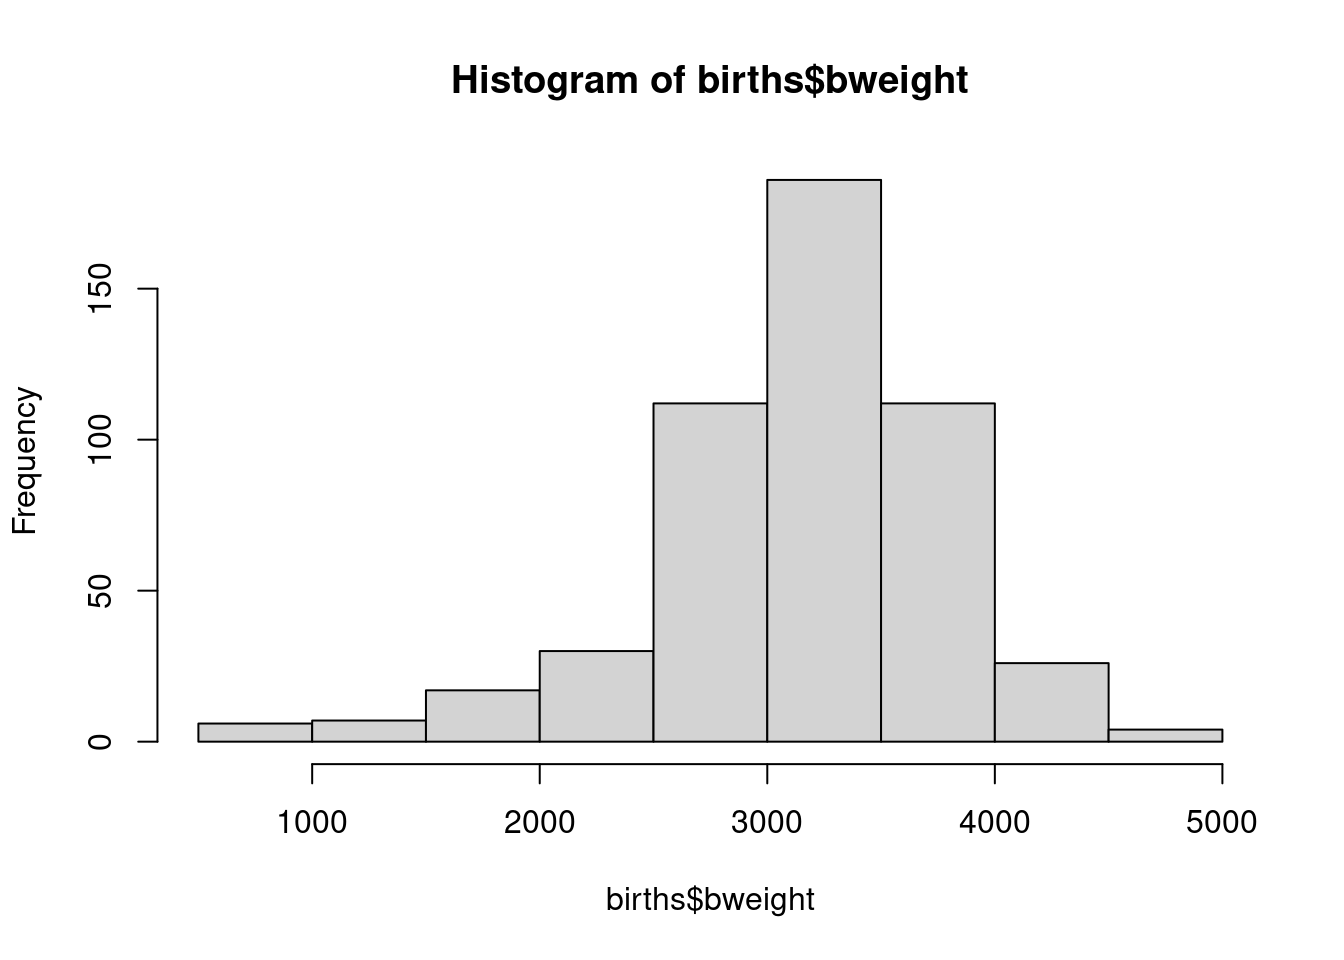
\includegraphics{graph-intro-s_files/figure-latex/unnamed-chunk-3-1.pdf}
The histogram can be refined -- take a look at the possible options with

\begin{Shaded}
\begin{Highlighting}[]
\FunctionTok{help}\NormalTok{(hist)}
\end{Highlighting}
\end{Shaded}

and try some of the options, for example:

\begin{Shaded}
\begin{Highlighting}[]
\FunctionTok{hist}\NormalTok{(births}\SpecialCharTok{$}\NormalTok{bweight, }\AttributeTok{col =} \StringTok{"gray"}\NormalTok{, }\AttributeTok{border =} \StringTok{"white"}\NormalTok{)}
\end{Highlighting}
\end{Shaded}

\includegraphics{graph-intro-s_files/figure-latex/unnamed-chunk-5-1.pdf}
To look at the relationship between birthweight and gestational weeks, try

\begin{Shaded}
\begin{Highlighting}[]
\FunctionTok{with}\NormalTok{(births, }\FunctionTok{plot}\NormalTok{(gestwks, bweight))}
\end{Highlighting}
\end{Shaded}

\includegraphics{graph-intro-s_files/figure-latex/unnamed-chunk-6-1.pdf}
You can change the plot-symbol by the option \texttt{pch=}. If you
want to see all the plot symbols try:

\begin{Shaded}
\begin{Highlighting}[]
\FunctionTok{plot}\NormalTok{(}\DecValTok{1}\SpecialCharTok{:}\DecValTok{25}\NormalTok{, }\AttributeTok{pch =} \DecValTok{1}\SpecialCharTok{:}\DecValTok{25}\NormalTok{)}
\end{Highlighting}
\end{Shaded}

\includegraphics{graph-intro-s_files/figure-latex/unnamed-chunk-7-1.pdf}

\begin{itemize}
\tightlist
\item
  Make a plot of the birth weight versus maternal age with
\end{itemize}

\begin{Shaded}
\begin{Highlighting}[]
\FunctionTok{with}\NormalTok{(births, }\FunctionTok{plot}\NormalTok{(matage, bweight))}
\end{Highlighting}
\end{Shaded}

\includegraphics{graph-intro-s_files/figure-latex/unnamed-chunk-8-1.pdf}
- Label the axes with

\begin{Shaded}
\begin{Highlighting}[]
\FunctionTok{with}\NormalTok{(}
\NormalTok{  births, }
  \FunctionTok{plot}\NormalTok{(}
\NormalTok{    matage, }
\NormalTok{    bweight, }
    \AttributeTok{xlab =} \StringTok{"Maternal age"}\NormalTok{, }
    \AttributeTok{ylab =} \StringTok{"Birth weight (g)"}
\NormalTok{  )}
\NormalTok{)}
\end{Highlighting}
\end{Shaded}

\includegraphics{graph-intro-s_files/figure-latex/unnamed-chunk-9-1.pdf}

\section{Colours}\label{colours}

There are many colours recognized by \texttt{R}. You can list them all by
\texttt{colours()} or, equivalently, \texttt{colors()} (\texttt{R} allows you to
use British or American spelling). To colour the points of birthweight
versus gestational weeks, try

\begin{Shaded}
\begin{Highlighting}[]
\FunctionTok{with}\NormalTok{(births, }\FunctionTok{plot}\NormalTok{(gestwks, bweight, }\AttributeTok{pch =} \DecValTok{16}\NormalTok{, }\AttributeTok{col =} \StringTok{"green"}\NormalTok{))}
\end{Highlighting}
\end{Shaded}

\includegraphics{graph-intro-s_files/figure-latex/unnamed-chunk-10-1.pdf}
This creates a solid mass of colour in the centre of the cluster of
points and it is no longer possible to see individual points. You can
recover this information by overwriting the points with black circles
using the \texttt{points()} function.

\begin{Shaded}
\begin{Highlighting}[]
\FunctionTok{with}\NormalTok{(births, }\FunctionTok{plot}\NormalTok{(gestwks, bweight, }\AttributeTok{pch =} \DecValTok{16}\NormalTok{, }\AttributeTok{col =} \StringTok{"green"}\NormalTok{))}
\FunctionTok{with}\NormalTok{(births, }\FunctionTok{points}\NormalTok{(gestwks, bweight, }\AttributeTok{pch =} \DecValTok{1}\NormalTok{))}
\end{Highlighting}
\end{Shaded}

\includegraphics{graph-intro-s_files/figure-latex/unnamed-chunk-11-1.pdf}
Note: when the number of data points on a scatter plot is large, you may also want to decrease the point size: to get points that are 50\% of the original size, add the parameter \texttt{cex=0.5} (or another number \textless1 for different sizes).

\section{Adding to a plot}\label{adding-to-a-plot}

The \texttt{points()} function just used is one of several functions
that add elements to an existing plot. By using these functions, you
can create quite complex graphs in small steps.

Suppose we wish to recreate the plot of birthweight \emph{vs} gestational
weeks using different colours for male and female babies. To start with
an empty plot, with \texttt{type=\textquotesingle{}n\textquotesingle{}} argument.

Then add the points with the \texttt{points} function.

\begin{Shaded}
\begin{Highlighting}[]
\FunctionTok{with}\NormalTok{(births, }\FunctionTok{plot}\NormalTok{(gestwks, bweight, }\AttributeTok{type =} \StringTok{"n"}\NormalTok{))}
\FunctionTok{with}\NormalTok{(}
\NormalTok{  births, }
  \FunctionTok{points}\NormalTok{(gestwks[sex }\SpecialCharTok{==} \DecValTok{1}\NormalTok{], bweight[sex }\SpecialCharTok{==} \DecValTok{1}\NormalTok{], }\AttributeTok{col =} \StringTok{"blue"}\NormalTok{)}
\NormalTok{)}
\FunctionTok{with}\NormalTok{(}
\NormalTok{  births, }
  \FunctionTok{points}\NormalTok{(gestwks[sex }\SpecialCharTok{==} \DecValTok{2}\NormalTok{], bweight[sex }\SpecialCharTok{==} \DecValTok{2}\NormalTok{], }\AttributeTok{col =} \StringTok{"red"}\NormalTok{)}
\NormalTok{)}
\end{Highlighting}
\end{Shaded}

\includegraphics{graph-intro-s_files/figure-latex/unnamed-chunk-12-1.pdf}

To add a legend explaining the colours, try

\begin{Shaded}
\begin{Highlighting}[]
\FunctionTok{with}\NormalTok{(births, }\FunctionTok{plot}\NormalTok{(gestwks, bweight, }\AttributeTok{type =} \StringTok{"n"}\NormalTok{))}
\FunctionTok{with}\NormalTok{(}
\NormalTok{  births, }
  \FunctionTok{points}\NormalTok{(gestwks[sex }\SpecialCharTok{==} \DecValTok{1}\NormalTok{], bweight[sex }\SpecialCharTok{==} \DecValTok{1}\NormalTok{], }\AttributeTok{col =} \StringTok{"blue"}\NormalTok{)}
\NormalTok{)}
\FunctionTok{with}\NormalTok{(}
\NormalTok{  births, }
  \FunctionTok{points}\NormalTok{(gestwks[sex }\SpecialCharTok{==} \DecValTok{2}\NormalTok{], bweight[sex }\SpecialCharTok{==} \DecValTok{2}\NormalTok{], }\AttributeTok{col =} \StringTok{"red"}\NormalTok{)}
\NormalTok{)}
\FunctionTok{legend}\NormalTok{(}
  \StringTok{"topleft"}\NormalTok{, }
  \AttributeTok{pch =} \DecValTok{1}\NormalTok{, }
  \AttributeTok{legend =} \FunctionTok{c}\NormalTok{(}\StringTok{"Boys"}\NormalTok{, }\StringTok{"Girls"}\NormalTok{), }
  \AttributeTok{col =} \FunctionTok{c}\NormalTok{(}\StringTok{"blue"}\NormalTok{, }\StringTok{"red"}\NormalTok{)}
\NormalTok{)}
\end{Highlighting}
\end{Shaded}

\includegraphics{graph-intro-s_files/figure-latex/unnamed-chunk-13-1.pdf}
which puts the legend in the top left hand corner.

Finally we can add a title to the plot with

\begin{Shaded}
\begin{Highlighting}[]
\FunctionTok{with}\NormalTok{(births, }\FunctionTok{plot}\NormalTok{(gestwks, bweight, }\AttributeTok{type =} \StringTok{"n"}\NormalTok{))}
\FunctionTok{with}\NormalTok{(}
\NormalTok{  births, }
  \FunctionTok{points}\NormalTok{(gestwks[sex }\SpecialCharTok{==} \DecValTok{1}\NormalTok{], bweight[sex }\SpecialCharTok{==} \DecValTok{1}\NormalTok{], }\AttributeTok{col =} \StringTok{"blue"}\NormalTok{)}
\NormalTok{)}
\FunctionTok{with}\NormalTok{(}
\NormalTok{  births, }
  \FunctionTok{points}\NormalTok{(gestwks[sex }\SpecialCharTok{==} \DecValTok{2}\NormalTok{], bweight[sex }\SpecialCharTok{==} \DecValTok{2}\NormalTok{], }\AttributeTok{col =} \StringTok{"red"}\NormalTok{)}
\NormalTok{)}
\FunctionTok{legend}\NormalTok{(}
  \StringTok{"topleft"}\NormalTok{, }
  \AttributeTok{pch =} \DecValTok{1}\NormalTok{, }
  \AttributeTok{legend =} \FunctionTok{c}\NormalTok{(}\StringTok{"Boys"}\NormalTok{, }\StringTok{"Girls"}\NormalTok{), }
  \AttributeTok{col =} \FunctionTok{c}\NormalTok{(}\StringTok{"blue"}\NormalTok{, }\StringTok{"red"}\NormalTok{)}
\NormalTok{)}
\FunctionTok{title}\NormalTok{(}
  \StringTok{"Birth weight vs gestational weeks in 500 singleton births"}
\NormalTok{)}
\end{Highlighting}
\end{Shaded}

\includegraphics{graph-intro-s_files/figure-latex/unnamed-chunk-14-1.pdf}

\section{Using indexing for plot elements}\label{using-indexing-for-plot-elements}

One of the most powerful features of R is the possibility to index
vectors, not only to get subsets of them, but also for repeating their
elements in complex sequences.

Putting separate colours on males and female as above would become
very clumsy if we had a 5 level factor instead of sex.

Instead of specifying one color for all points, we may specify a
vector of colours of the same length as the \texttt{gestwks} and
\texttt{bweight} vectors. This is rather tedious to do directly, but R
allows you to specify an expression anywhere, so we can use the fact
that \texttt{sex} takes the values 1 and 2, as follows:

First create a colour vector with two colours,
and take look at \texttt{sex}:

\begin{Shaded}
\begin{Highlighting}[]
\FunctionTok{c}\NormalTok{(}\StringTok{"blue"}\NormalTok{, }\StringTok{"red"}\NormalTok{)}
\end{Highlighting}
\end{Shaded}

\begin{verbatim}
## [1] "blue" "red"
\end{verbatim}

\begin{Shaded}
\begin{Highlighting}[]
\NormalTok{births}\SpecialCharTok{$}\NormalTok{sex}
\end{Highlighting}
\end{Shaded}

\begin{verbatim}
##   [1] 2 1 2 1 1 2 2 1 2 1 1 2 2 1 2 1 2 1 2 2 2 1 2 2 2 1 2 1 2 1 2 2 1 1 2 2 1
##  [38] 1 2 1 2 1 1 1 1 1 1 1 1 1 1 2 1 2 1 1 1 1 1 1 2 1 1 2 1 1 2 2 1 2 1 1 1 1
##  [75] 1 2 1 1 2 1 2 1 1 2 1 1 1 2 1 1 1 2 1 2 1 1 2 1 2 2 2 2 2 2 2 1 1 2 2 2 1
## [112] 2 2 1 2 2 2 2 1 1 2 1 1 2 1 1 2 1 2 1 1 1 1 2 1 2 1 1 1 2 1 2 2 1 1 1 2 2
## [149] 2 2 2 2 1 2 1 1 2 1 1 2 2 1 2 1 1 1 1 1 2 1 1 2 2 1 1 1 2 2 2 2 1 2 1 2 1
## [186] 1 2 2 1 2 2 1 2 1 2 2 2 2 1 1 1 2 1 1 2 1 1 1 1 2 2 2 2 2 1 1 2 1 2 2 2 1
## [223] 2 1 1 1 1 2 1 2 2 2 1 2 2 2 1 1 2 1 1 2 1 2 2 2 1 1 2 2 2 2 1 1 1 2 2 1 2
## [260] 2 2 2 1 1 1 1 1 1 2 1 2 1 2 2 2 2 2 1 1 1 2 2 2 1 2 1 2 1 2 1 1 1 2 2 2 2
## [297] 1 2 1 1 2 1 2 1 1 2 1 2 1 2 2 1 1 2 1 1 2 1 1 2 2 1 1 1 1 2 2 2 2 1 1 1 1
## [334] 2 1 1 2 2 1 2 2 1 1 2 1 1 2 1 2 1 1 1 1 2 1 1 2 2 2 1 1 1 1 1 1 2 2 2 2 2
## [371] 1 1 2 1 1 2 1 2 1 1 1 2 2 1 1 2 1 1 1 2 1 1 1 1 1 1 1 2 2 1 2 2 1 2 2 1 1
## [408] 2 2 1 1 2 1 1 2 1 2 1 2 2 1 1 2 2 1 2 2 2 2 1 1 2 2 2 2 2 2 1 2 1 1 2 2 1
## [445] 1 1 2 2 2 2 1 2 2 2 2 1 1 2 1 2 1 1 1 1 2 1 1 1 2 1 2 1 1 1 1 2 2 1 2 1 2
## [482] 2 1 1 2 2 1 1 1 1 2 2 2 1 1 2 1 2 2 1
\end{verbatim}

Now see what happens if you index the colour vector by sex:

\begin{Shaded}
\begin{Highlighting}[]
\FunctionTok{c}\NormalTok{(}\StringTok{"blue"}\NormalTok{, }\StringTok{"red"}\NormalTok{)[births}\SpecialCharTok{$}\NormalTok{sex]}
\end{Highlighting}
\end{Shaded}

\begin{verbatim}
##   [1] "red"  "blue" "red"  "blue" "blue" "red"  "red"  "blue" "red"  "blue"
##  [11] "blue" "red"  "red"  "blue" "red"  "blue" "red"  "blue" "red"  "red" 
##  [21] "red"  "blue" "red"  "red"  "red"  "blue" "red"  "blue" "red"  "blue"
##  [31] "red"  "red"  "blue" "blue" "red"  "red"  "blue" "blue" "red"  "blue"
##  [41] "red"  "blue" "blue" "blue" "blue" "blue" "blue" "blue" "blue" "blue"
##  [51] "blue" "red"  "blue" "red"  "blue" "blue" "blue" "blue" "blue" "blue"
##  [61] "red"  "blue" "blue" "red"  "blue" "blue" "red"  "red"  "blue" "red" 
##  [71] "blue" "blue" "blue" "blue" "blue" "red"  "blue" "blue" "red"  "blue"
##  [81] "red"  "blue" "blue" "red"  "blue" "blue" "blue" "red"  "blue" "blue"
##  [91] "blue" "red"  "blue" "red"  "blue" "blue" "red"  "blue" "red"  "red" 
## [101] "red"  "red"  "red"  "red"  "red"  "blue" "blue" "red"  "red"  "red" 
## [111] "blue" "red"  "red"  "blue" "red"  "red"  "red"  "red"  "blue" "blue"
## [121] "red"  "blue" "blue" "red"  "blue" "blue" "red"  "blue" "red"  "blue"
## [131] "blue" "blue" "blue" "red"  "blue" "red"  "blue" "blue" "blue" "red" 
## [141] "blue" "red"  "red"  "blue" "blue" "blue" "red"  "red"  "red"  "red" 
## [151] "red"  "red"  "blue" "red"  "blue" "blue" "red"  "blue" "blue" "red" 
## [161] "red"  "blue" "red"  "blue" "blue" "blue" "blue" "blue" "red"  "blue"
## [171] "blue" "red"  "red"  "blue" "blue" "blue" "red"  "red"  "red"  "red" 
## [181] "blue" "red"  "blue" "red"  "blue" "blue" "red"  "red"  "blue" "red" 
## [191] "red"  "blue" "red"  "blue" "red"  "red"  "red"  "red"  "blue" "blue"
## [201] "blue" "red"  "blue" "blue" "red"  "blue" "blue" "blue" "blue" "red" 
## [211] "red"  "red"  "red"  "red"  "blue" "blue" "red"  "blue" "red"  "red" 
## [221] "red"  "blue" "red"  "blue" "blue" "blue" "blue" "red"  "blue" "red" 
## [231] "red"  "red"  "blue" "red"  "red"  "red"  "blue" "blue" "red"  "blue"
## [241] "blue" "red"  "blue" "red"  "red"  "red"  "blue" "blue" "red"  "red" 
## [251] "red"  "red"  "blue" "blue" "blue" "red"  "red"  "blue" "red"  "red" 
## [261] "red"  "red"  "blue" "blue" "blue" "blue" "blue" "blue" "red"  "blue"
## [271] "red"  "blue" "red"  "red"  "red"  "red"  "red"  "blue" "blue" "blue"
## [281] "red"  "red"  "red"  "blue" "red"  "blue" "red"  "blue" "red"  "blue"
## [291] "blue" "blue" "red"  "red"  "red"  "red"  "blue" "red"  "blue" "blue"
## [301] "red"  "blue" "red"  "blue" "blue" "red"  "blue" "red"  "blue" "red" 
## [311] "red"  "blue" "blue" "red"  "blue" "blue" "red"  "blue" "blue" "red" 
## [321] "red"  "blue" "blue" "blue" "blue" "red"  "red"  "red"  "red"  "blue"
## [331] "blue" "blue" "blue" "red"  "blue" "blue" "red"  "red"  "blue" "red" 
## [341] "red"  "blue" "blue" "red"  "blue" "blue" "red"  "blue" "red"  "blue"
## [351] "blue" "blue" "blue" "red"  "blue" "blue" "red"  "red"  "red"  "blue"
## [361] "blue" "blue" "blue" "blue" "blue" "red"  "red"  "red"  "red"  "red" 
## [371] "blue" "blue" "red"  "blue" "blue" "red"  "blue" "red"  "blue" "blue"
## [381] "blue" "red"  "red"  "blue" "blue" "red"  "blue" "blue" "blue" "red" 
## [391] "blue" "blue" "blue" "blue" "blue" "blue" "blue" "red"  "red"  "blue"
## [401] "red"  "red"  "blue" "red"  "red"  "blue" "blue" "red"  "red"  "blue"
## [411] "blue" "red"  "blue" "blue" "red"  "blue" "red"  "blue" "red"  "red" 
## [421] "blue" "blue" "red"  "red"  "blue" "red"  "red"  "red"  "red"  "blue"
## [431] "blue" "red"  "red"  "red"  "red"  "red"  "red"  "blue" "red"  "blue"
## [441] "blue" "red"  "red"  "blue" "blue" "blue" "red"  "red"  "red"  "red" 
## [451] "blue" "red"  "red"  "red"  "red"  "blue" "blue" "red"  "blue" "red" 
## [461] "blue" "blue" "blue" "blue" "red"  "blue" "blue" "blue" "red"  "blue"
## [471] "red"  "blue" "blue" "blue" "blue" "red"  "red"  "blue" "red"  "blue"
## [481] "red"  "red"  "blue" "blue" "red"  "red"  "blue" "blue" "blue" "blue"
## [491] "red"  "red"  "red"  "blue" "blue" "red"  "blue" "red"  "red"  "blue"
\end{verbatim}

For every occurrence of a \texttt{1} in \texttt{sex} you get
\texttt{"blue"}, and for every occurrence of \texttt{2} you get
\texttt{"red"}, so the result is a long vector of \texttt{"blue"}s and
\texttt{"red"}s corresponding to the males and females.
This can now be used in the plot:

\begin{Shaded}
\begin{Highlighting}[]
\FunctionTok{with}\NormalTok{(}
\NormalTok{  births, }
  \FunctionTok{plot}\NormalTok{(gestwks, bweight, }\AttributeTok{pch =} \DecValTok{16}\NormalTok{, }\AttributeTok{col =} \FunctionTok{c}\NormalTok{(}\StringTok{"blue"}\NormalTok{, }\StringTok{"red"}\NormalTok{)[sex])}
\NormalTok{)}
\end{Highlighting}
\end{Shaded}

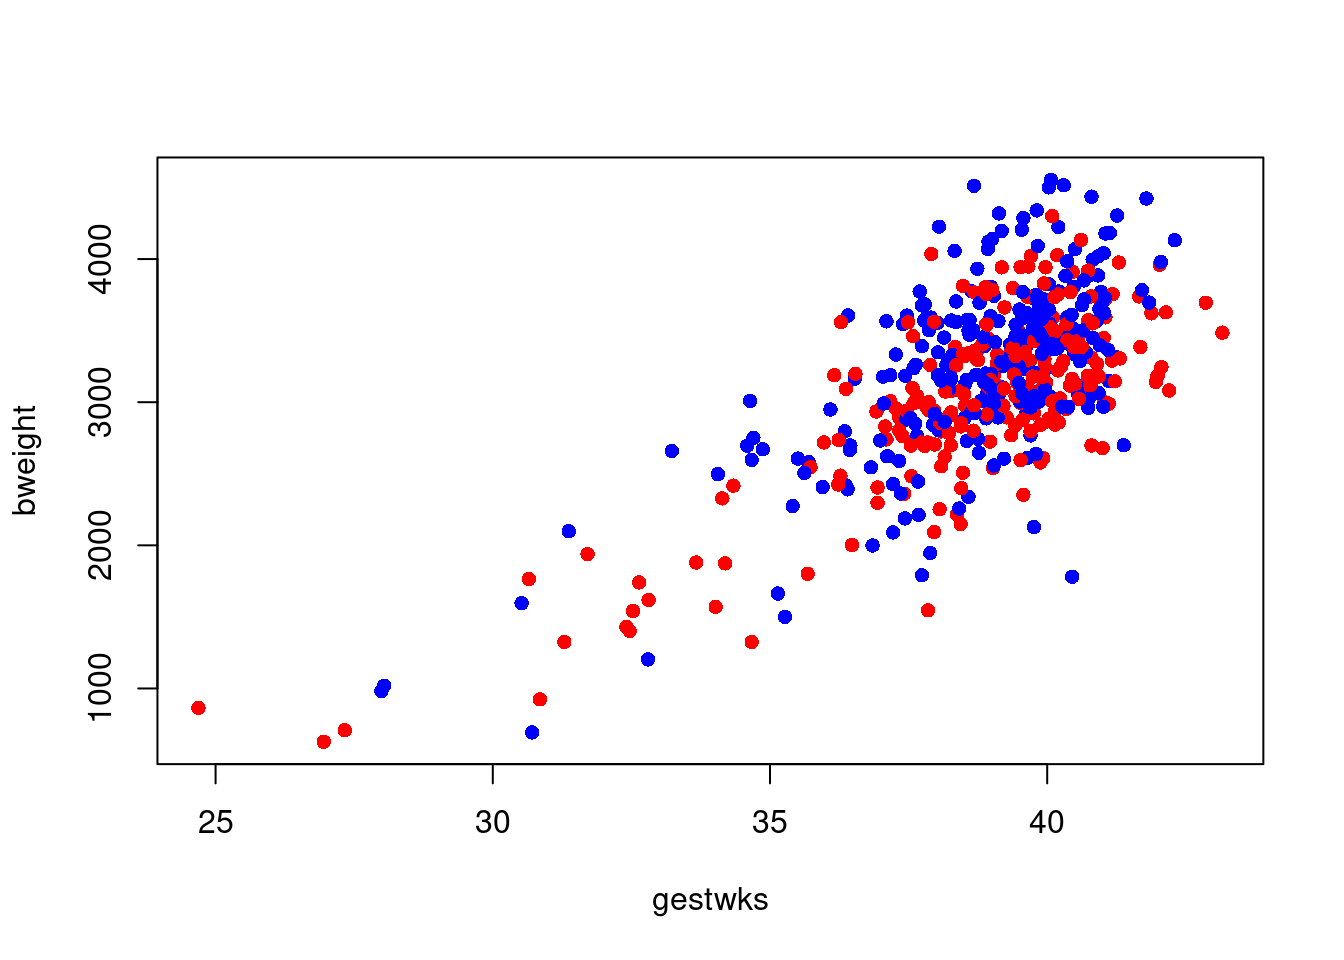
\includegraphics{graph-intro-s_files/figure-latex/unnamed-chunk-17-1.pdf}
The same trick can be used if we want to have a separate symbol for
mothers over 40 say. We first generate the indexing variable:

\begin{Shaded}
\begin{Highlighting}[]
\NormalTok{births}\SpecialCharTok{$}\NormalTok{oldmum }\OtherTok{\textless{}{-}}\NormalTok{ (births}\SpecialCharTok{$}\NormalTok{matage }\SpecialCharTok{\textgreater{}=} \DecValTok{40}\NormalTok{) }\SpecialCharTok{+} \DecValTok{1}
\end{Highlighting}
\end{Shaded}

Note we add 1 because \texttt{(\ matage\ \textgreater{}=\ 40\ )} generates a logic
variable, so by adding 1 we get a numeric variable with values 1 and
2, suitable for indexing:

\begin{Shaded}
\begin{Highlighting}[]
\FunctionTok{with}\NormalTok{(}
\NormalTok{  births, }
  \FunctionTok{plot}\NormalTok{(}
\NormalTok{    gestwks, }
\NormalTok{    bweight, }
    \AttributeTok{pch =} \FunctionTok{c}\NormalTok{(}\DecValTok{16}\NormalTok{, }\DecValTok{3}\NormalTok{)[oldmum], }
    \AttributeTok{col =} \FunctionTok{c}\NormalTok{(}\StringTok{"blue"}\NormalTok{, }\StringTok{"red"}\NormalTok{)[sex]}
\NormalTok{  )}
\NormalTok{)}
\end{Highlighting}
\end{Shaded}

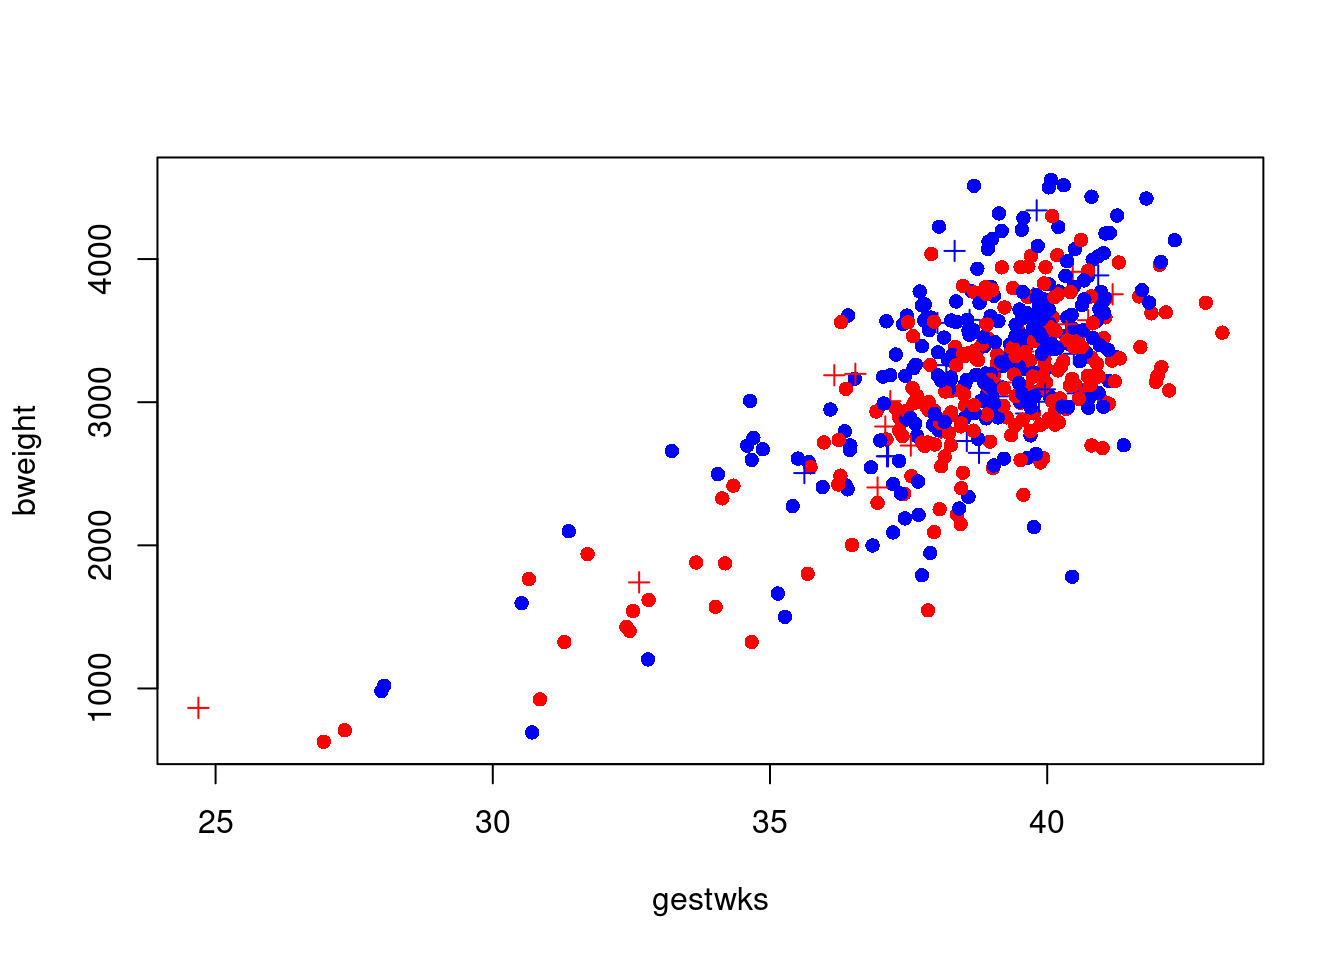
\includegraphics{graph-intro-s_files/figure-latex/unnamed-chunk-19-1.pdf}
so where \texttt{oldmum} is 1 we get \texttt{pch=16} (a dot) and where
\texttt{oldmum} is 2 we get \texttt{pch=3} (a cross).

R will accept any kind of complexity in the indexing as
long as the result is a valid index, so you don't need to create the
variable \texttt{oldmum}, you can create it on the fly:

\begin{Shaded}
\begin{Highlighting}[]
\FunctionTok{with}\NormalTok{(}
\NormalTok{  births, }
  \FunctionTok{plot}\NormalTok{(}
\NormalTok{    gestwks, }
\NormalTok{    bweight, }
    \AttributeTok{pch =} \FunctionTok{c}\NormalTok{(}\DecValTok{16}\NormalTok{, }\DecValTok{3}\NormalTok{)[(matage }\SpecialCharTok{\textgreater{}=} \DecValTok{40}\NormalTok{) }\SpecialCharTok{+} \DecValTok{1}\NormalTok{], }
    \AttributeTok{col =} \FunctionTok{c}\NormalTok{(}\StringTok{"blue"}\NormalTok{, }\StringTok{"red"}\NormalTok{)[sex]}
\NormalTok{  )}
\NormalTok{)}
\end{Highlighting}
\end{Shaded}

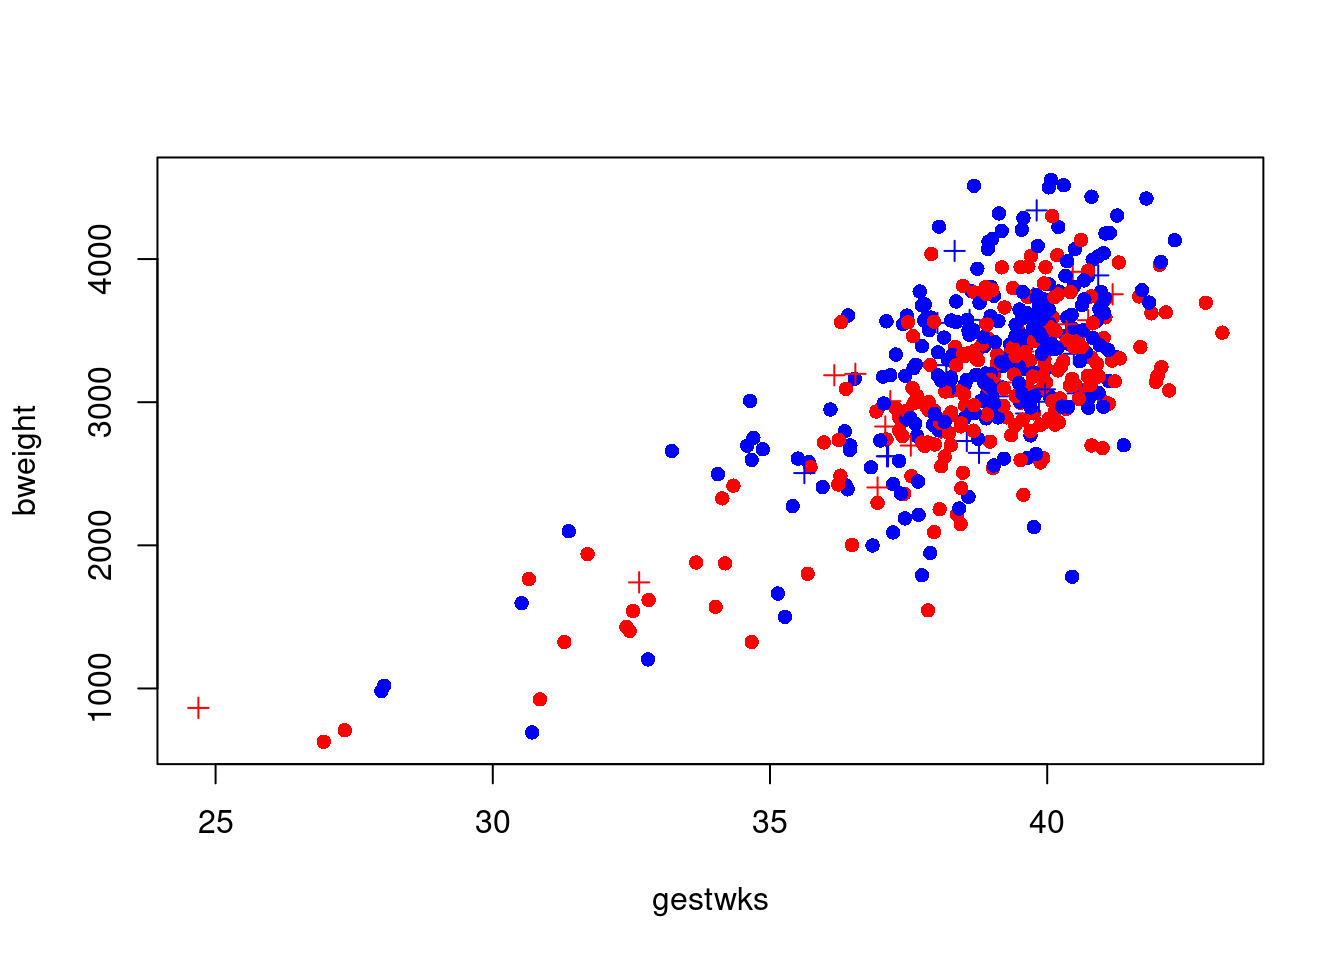
\includegraphics{graph-intro-s_files/figure-latex/unnamed-chunk-20-1.pdf}

\section{Generating colours}\label{generating-colours}

R has functions that generate a vector of colours for you. For example,

\begin{Shaded}
\begin{Highlighting}[]
\FunctionTok{rainbow}\NormalTok{(}\DecValTok{4}\NormalTok{)}
\end{Highlighting}
\end{Shaded}

\begin{verbatim}
## [1] "#FF0000" "#80FF00" "#00FFFF" "#8000FF"
\end{verbatim}

produces a vector with 4 colours (not immediately human readable,
though). There are a few other functions that generates other
sequences of colours, type \texttt{?rainbow} to see them. The
\texttt{color} function (or \texttt{colour} function if you prefer)
returns a vector of the colour names that R knows about. These
names can also be used to specify colours.

Gray-tones are produced by the function \texttt{gray} (or
\texttt{grey}), which takes a numerical argument between 0 and 1;
\texttt{gray(0)} is black and \texttt{gray(1)} is white. Try:

\begin{Shaded}
\begin{Highlighting}[]
\FunctionTok{plot}\NormalTok{(}\DecValTok{0}\SpecialCharTok{:}\DecValTok{10}\NormalTok{, }\AttributeTok{pch =} \DecValTok{16}\NormalTok{, }\AttributeTok{cex =} \DecValTok{3}\NormalTok{, }\AttributeTok{col =} \FunctionTok{gray}\NormalTok{(}\DecValTok{0}\SpecialCharTok{:}\DecValTok{10} \SpecialCharTok{/} \DecValTok{10}\NormalTok{))}
\FunctionTok{points}\NormalTok{(}\DecValTok{0}\SpecialCharTok{:}\DecValTok{10}\NormalTok{, }\AttributeTok{pch =} \DecValTok{1}\NormalTok{, }\AttributeTok{cex =} \DecValTok{3}\NormalTok{)}
\end{Highlighting}
\end{Shaded}

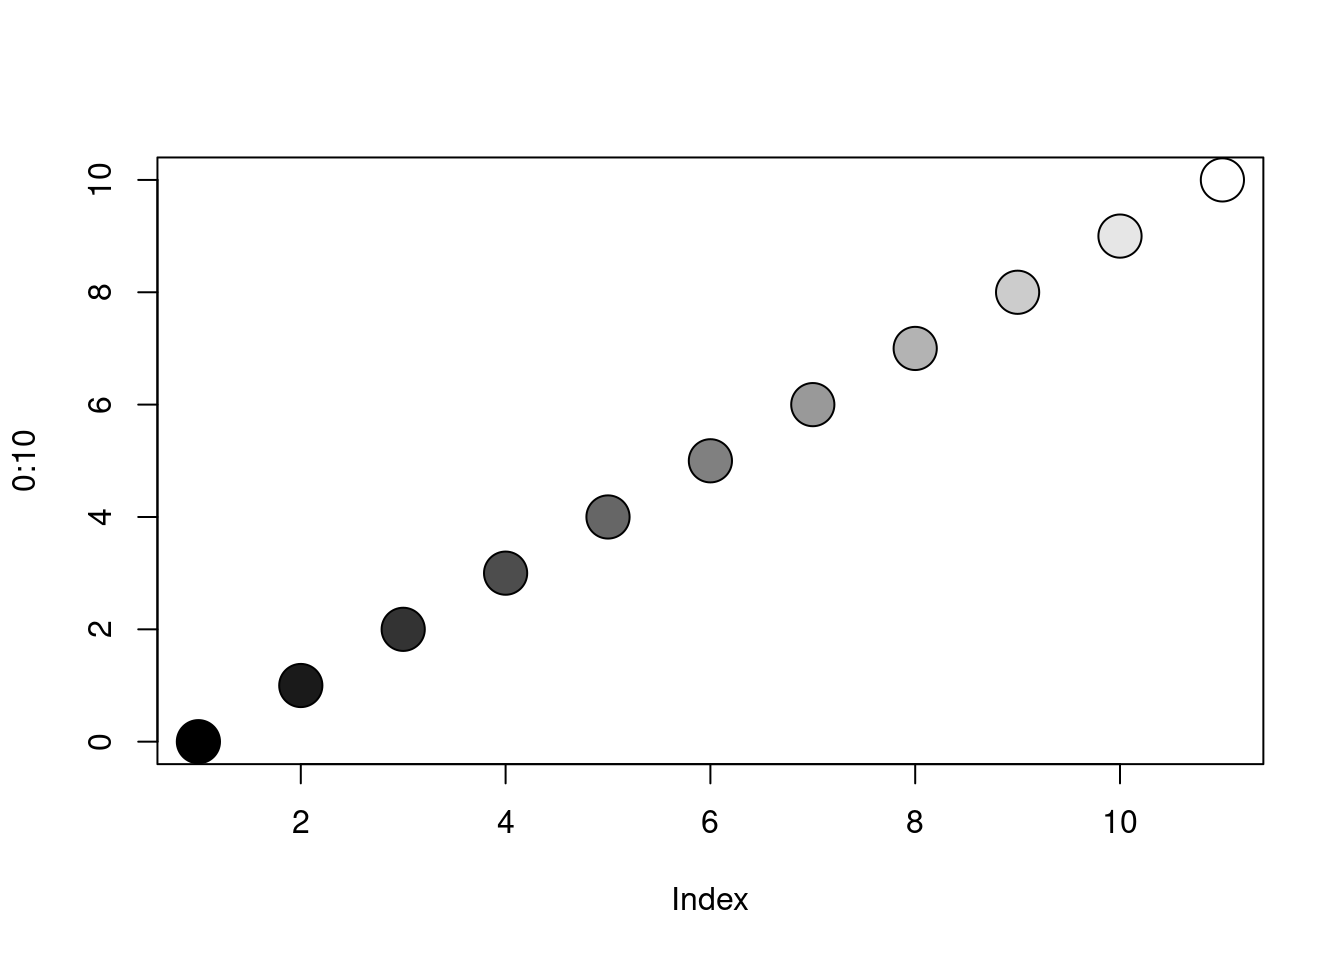
\includegraphics{graph-intro-s_files/figure-latex/unnamed-chunk-22-1.pdf}

\section{Saving your graphs for use in other documents}\label{saving-your-graphs-for-use-in-other-documents}

If you need to use the plot in a report or presentation, you can save it in a graphics file.
Once you have generated the script (sequence of R commands) that produce the graph (and it looks ok on screen),
you can start a non-interactive graphics device and then re-run the script.
Instead of appearing on the screen, the plot will now be written
directly to a file. After the plot has been completed you will need
to close the device again in order to be able to access the file. Try:

\begin{Shaded}
\begin{Highlighting}[]
\FunctionTok{pdf}\NormalTok{(}\AttributeTok{file =} \StringTok{"bweight\_gwks.pdf"}\NormalTok{, }\AttributeTok{height =} \DecValTok{4}\NormalTok{, }\AttributeTok{width =} \DecValTok{4}\NormalTok{)}
\FunctionTok{with}\NormalTok{(births, }\FunctionTok{plot}\NormalTok{(gestwks, bweight, }\AttributeTok{col =} \FunctionTok{c}\NormalTok{(}\StringTok{"blue"}\NormalTok{, }\StringTok{"red"}\NormalTok{)[sex]))}
\FunctionTok{legend}\NormalTok{(}
  \StringTok{"topleft"}\NormalTok{, }
  \AttributeTok{pch =} \DecValTok{1}\NormalTok{, }
  \AttributeTok{legend =} \FunctionTok{c}\NormalTok{(}\StringTok{"Boys"}\NormalTok{, }\StringTok{"Girls"}\NormalTok{), }
  \AttributeTok{col =} \FunctionTok{c}\NormalTok{(}\StringTok{"blue"}\NormalTok{, }\StringTok{"red"}\NormalTok{)}
\NormalTok{)}
\FunctionTok{dev.off}\NormalTok{()}
\end{Highlighting}
\end{Shaded}

This will give you a portable document file \texttt{bweight\_gwks.pdf} with a graph
which is 4 inches tall and 4 inches wide.

Instead of \emph{pdf}, other formats can be used (\emph{jpg, png, tiff, \ldots{}}). See \texttt{help(Devices)} for the available options.

In window-based environments (R GUI for Windows, R-Studio) you may also use the menu
(\texttt{File}\(\rightarrow\)\texttt{Save\ as\ ...} or \texttt{Export}) to save the active graph as a file and even copy-paste may work (from R graphics window to Word, for instance) -- however, writing it manually into the file is recommended for reproducibility purposes (in case you need to redraw your graph with some modifications).

\subsection{The `par()` command}

It is possible to manipulate any element in a graph, by using the
graphics options. These are collected on the help page of
\texttt{par()}. For example, if you want axis labels always to be
horizontal, use the command \texttt{par(las=1)}. This will be in
effect until a new graphics device is opened.

Look at the typewriter-version of the help-page with

\begin{Shaded}
\begin{Highlighting}[]
\FunctionTok{help}\NormalTok{(par)}
\end{Highlighting}
\end{Shaded}

or better, use the the html-version through
\texttt{Help} \(\rightarrow\) \texttt{Html\ help} \(\rightarrow\)
\texttt{Packages} \(\rightarrow\) \texttt{graphics} \(\rightarrow\)
\texttt{P}\(\rightarrow\) \texttt{par}.

It is a good idea to take a print of this (having set the text
size to \emph{smallest} because it is long) and carry it with you at any
time to read in buses, cinema queues, during boring lectures etc.
Don't despair, few R-users can understand what all the options are
for.

\texttt{par()} can also be used to ask about the current plot, for
example \texttt{par("usr")} will give you the exact extent of the axes
in the current plot.

If you want more plots on a single page you can use the command

\begin{Shaded}
\begin{Highlighting}[]
\FunctionTok{par}\NormalTok{(}\AttributeTok{mfrow =} \FunctionTok{c}\NormalTok{(}\DecValTok{2}\NormalTok{, }\DecValTok{3}\NormalTok{))}
\end{Highlighting}
\end{Shaded}

This will give you a layout of 2 rows by 3 columns for the next 6
graphs you produce. The plots will appear by row, i.e.~in the top
row first. If you want the plots to appear columnwise, use
\texttt{par(\ mfcol=c(2,3)\ )} (you still get 2 rows by 3 columns).

To restore the layout to a single plot per page use

\begin{Shaded}
\begin{Highlighting}[]
\FunctionTok{par}\NormalTok{(}\AttributeTok{mfrow =} \FunctionTok{c}\NormalTok{(}\DecValTok{1}\NormalTok{, }\DecValTok{1}\NormalTok{))}
\end{Highlighting}
\end{Shaded}

If you want a more detailed control over the layout of multiple graphs
on a single page look at \texttt{?layout}.

\section{Interacting with a plot}\label{interacting-with-a-plot}

The \texttt{locator()} function allows you to interact with the plot
using the mouse. Typing \texttt{locator(1)} shifts you to the graphics
window and waits for one click of the left mouse button. When you click,
it will return the corresponding coordinates.

You can use \texttt{locator()} inside other graphics functions to position
graphical elements exactly where you want them. Recreate the birth-weight
plot,

\begin{Shaded}
\begin{Highlighting}[]
\FunctionTok{with}\NormalTok{(births, }\FunctionTok{plot}\NormalTok{(gestwks, bweight, }\AttributeTok{col =} \FunctionTok{c}\NormalTok{(}\StringTok{"blue"}\NormalTok{, }\StringTok{"red"}\NormalTok{)[sex]))}
\end{Highlighting}
\end{Shaded}

\includegraphics{graph-intro-s_files/figure-latex/unnamed-chunk-27-1.pdf}
and then add the legend where you wish it to appear by typing

\begin{Shaded}
\begin{Highlighting}[]
\FunctionTok{legend}\NormalTok{(}
  \FunctionTok{locator}\NormalTok{(}\DecValTok{1}\NormalTok{), }
  \AttributeTok{pch =} \DecValTok{1}\NormalTok{, }
  \AttributeTok{legend =} \FunctionTok{c}\NormalTok{(}\StringTok{"Boys"}\NormalTok{, }\StringTok{"Girls"}\NormalTok{), }
  \AttributeTok{col =} \FunctionTok{c}\NormalTok{(}\StringTok{"blue"}\NormalTok{, }\StringTok{"red"}\NormalTok{)}
\NormalTok{)}
\end{Highlighting}
\end{Shaded}

The \texttt{identify()} function allows you to find out which records
in the data correspond to points on the graph. Try

\begin{Shaded}
\begin{Highlighting}[]
\FunctionTok{with}\NormalTok{(births, }\FunctionTok{identify}\NormalTok{(gestwks, bweight))}
\end{Highlighting}
\end{Shaded}

When you click the left mouse button, a label will appear on the graph
identifying the row number of the nearest point in the data frame
\texttt{births}. If there is no point nearby, \texttt{R} will print a warning
message on the console instead. To end the interaction with the
graphics window, right click the mouse: the \texttt{identify} function
returns a vector of identified points.

\begin{itemize}
\tightlist
\item
  Use \texttt{identify()} to find which records correspond to the
  smallest and largest number of gestational weeks and view the
  corresponding records:
\end{itemize}

\begin{Shaded}
\begin{Highlighting}[]
\FunctionTok{with}\NormalTok{(births, births[}\FunctionTok{identify}\NormalTok{(gestwks, bweight), ])}
\end{Highlighting}
\end{Shaded}

\chapter{Analysis of hazard rates, their ratios and differences and binary regression}\label{analysis-of-hazard-rates-their-ratios-and-differences-and-binary-regression}

This exercise is \emph{very} prescriptive, so you should make an
effort to really understand everything you type into R. Consult the
relevant slides of the lecture on \emph{Poisson and Binary regression \ldots{}}

\section{Hand calculations for a single rate}\label{hand-calculations-for-a-single-rate}

Let \(\lambda\) be the true \textbf{hazard rate} or theoretical incidence rate of a given outcome event.
Its estimator is the empirical \textbf{incidence rate}
\(\widehat\lambda = D/Y\) = no. cases/person-years. Recall that the
standard error of the empirical rate is
SE\((\widehat\lambda) = \widehat\lambda/\sqrt{D}\).

The simplest approximate 95\% confidence interval (CI) for \(\lambda\)
is given by
\[ \widehat\lambda \pm 1.96 \times SE(\widehat\lambda) \]

\begin{itemize}
\tightlist
\item
  Suppose \(15\) outcome events are observed during \(5532\) person-years in a given study cohort.
  Let's use R as a simple desk calculator to estimate the underlying hazard rate \(\lambda\) (in 1000
  person-years; therefore 5.532) and to get the first version of an approximate confidence
  interval:
\end{itemize}

\section{Poisson model for a single rate with logarithmic link}\label{poisson-model-for-a-single-rate-with-logarithmic-link}

You are able to estimate the hazard rate \(\lambda\) and compute its CI with a \textbf{Poisson regression model}, as described in the relevant slides in the lecture handout.

Poisson regression is a \textbf{generalized linear model} in which the \textbf{family}, \emph{i.e.} the distribution of the response variable, is assumed to be the Poisson distribution. The most commonly applied \textbf{link function}
in Poisson regression is the natural logarithm; log for short.

\begin{itemize}
\item
  A family object \texttt{poisreg}, a modified version of the original \texttt{poisson} family object, is available
  in package \texttt{Epi}. When using this, the response is defined as a \emph{matrix} of two columns: numbers
  of cases \(D\) and person-years \(Y\), these being combined into a matrix by \texttt{cbind(D,Y)}. No specification
  of \texttt{offset} is needed.
\item
  If you want confidence interval for log rate
\end{itemize}

In this course we endorse the use of family \texttt{poisreg} because of its advantages in more general settings.

\section{Poisson model for a single rate with identity link}\label{poisson-model-for-a-single-rate-with-identity-link}

The approach leaning on having the number of cases \(D\) as the response and log\((Y)\) as an offset,
is limited only to models with log link. A major advantage of the \texttt{poisreg} family is that it allows
a straighforward use of the \emph{identity} link, too. With this link the response variable is the same, but
the parameters to be directly estimated are now the rates itself and their differences, not the log-rates
and their differences as with the log link.

\begin{itemize}
\tightlist
\item
  Fit a Poisson model with identity link to our simple data, and
  use \texttt{ci.lin()} to produce the estimate and the
  confidence interval for the hazard rate from this model:
\end{itemize}

How is the coefficient of this model interpreted?
Verify that you actually get the same rate estimate and CI as in section 1.6.1, item 1.

\section{Poisson model assuming the same rate for several periods}\label{poisson-model-assuming-the-same-rate-for-several-periods}

Now, suppose the events and person years are collected over three distinct periods.

\begin{itemize}
\item
  Read in the data and compute period-specific rates
\item
  Using these data,
  fit the same model with log link as in section 1.6.2, assuming a common single hazard \(\lambda\)
  for the separate periods. Compare the result from the previous ones
\item
  Now test whether the rates are the same in the three periods:
  Try to fit a model with the period as a factor in the model:
\end{itemize}

Compare the goodness-of-fit of the two models using \texttt{anova()} with the argument
\texttt{test="Chisq"}:

Compare the test statistic to the deviance of the model \texttt{mp}.
-- What is the deviance indicating?

\section{Analysis of rate ratio}\label{analysis-of-rate-ratio}

We now switch to comparison of two rates \(\lambda_1\) and \(\lambda_0\), i.e.
the hazard in an exposed group vs.~that in an unexposed one.

Consider first estimation of the \textbf{hazard ratio} or the underlying \emph{true} rate ratio
\(\rho = \lambda_1/\lambda_0\) between the groups. Suppose we have
pertinent empirical data (cases and person-times) from both groups,
\((D_1,Y_1)\) and \((D_0,Y_0)\). The point estimate of \(\rho\) is the
empirical \textbf{incidence rate ratio}
\[
\widehat{\rho} = RR = \frac{\widehat\lambda_1}{\widehat\lambda_0} = \frac{D_1/Y_1}{D_0/Y_0}
\]

Suppose you have \(15\) events during \(5532\) person-years in an
unexposed group and \(28\) events during \(4783\) person-years in an
exposed group:

\begin{itemize}
\item
  Calculate the incidence rates in the two groups, their ratio, and the CI of the true hazard ratio \(\rho\) by direct application of the above formulae:
\item
  Now achieve this using a Poisson model. For that we first combine
  the group-specific numbers into pertinent vectors and specify a factor to represent the contrast between the exposed and the unexposed group
\end{itemize}

What do the parameters mean in this model?

\begin{itemize}
\tightlist
\item
  You can extract the estimation results for exponentiated parameters in two ways, as before:
\end{itemize}

\section{Analysis of rate difference}\label{analysis-of-rate-difference}

For the \textbf{hazard difference} \(\delta = \lambda_1 - \lambda_0\),
the natural estimator is the \textbf{incidence rate difference}
\[ \widehat\delta = \widehat\lambda_1  - \widehat\lambda_0 = D_1/Y_1 - D_0/Y_0 = \mbox{RD} . \]
Its variance is just the sum of the variances of the two rates
\[ var(RD) = var(\widehat\lambda_1 ) + var( \widehat\lambda_0 ) =  D_1/Y_1^2 + D_0/Y_0^2 \]

\begin{itemize}
\item
  Use this formula to compute the point estimate of the rate difference \(\lambda\) and a 95\% confidence interval for it:
\item
  Verify that this is the confidence interval you get when you fit
  an additive model (obtained by identity link) with exposure as a factor:
\end{itemize}

\section{Binary regression}\label{binary-regression}

Explore the factors associated with risk of low birth weight
in 500 singleton births in a London Hospital. Indicator (lowbw) for birth weight less than 2500 g. Data available from the Epi package. Factors of interest are
maternal hypertension (hyp), mother's age at birth over 35 years and sex of the baby.

Load the \texttt{Epi} package and the data set and look at its content

\begin{itemize}
\item
  Because all variables are numeric we need first to do a little housekeeping.
  Two of them are directly converted into factors,
  and categorical versions are created of two continuous variables by function \texttt{cut()}.
\item
  Cross tabulate (dplyr) counts of children by hypertension and low birth weight.
  calculate (mutate) proportions of low birth weigth children by hypertension.
\item
  Estimate relative risk of low birth weight for mothers with hypertension compared to those without using binary regression.
\item
  Adjust relative risk of low birth and hypertension with the sex of children
\item
  Adjust relative risk of low birth and hypertension with the sex of children and mother beeing over 35 years.
\end{itemize}

\section{Optional/Homework: Hand calculations and calculations using matrix tools}\label{optionalhomework-hand-calculations-and-calculations-using-matrix-tools}

\begin{quote}
NB. This subsection requires some familiarity with matrix algebra. Do this only after you have done the other exercises of this session.
\end{quote}

First some basic hand calculations.

\begin{itemize}
\item
  Suppose \(15\) outcome events are observed during \(5532\) person-years in a given study cohort.
  Let's use R as a simple desk calculator to estimate the underlying hazard rate \(\lambda\) (in 1000
  person-years; therefore 5.532) and to get the first version of an approximate confidence
  interval:
\item
  Compute now the approximate confidence interval using the method
  based on log-transformation and compare the result with that in the previous item.
\item
  Calculate the incidence rates in the two groups, their ratio, and the\\
  CI of the true hazard ratio \(\rho\) by direct application of the above formulae:
\item
  Explore the function \texttt{ci.mat()}, which lets you use
  matrix multiplication (operator \texttt{\textquotesingle{}\%*\%\textquotesingle{}}
  in R) to produce a confidence interval from an estimate and its
  standard error (or CIs from whole columns of estimates and SEs):
\end{itemize}

As you see, this function returns a \(2\times 3\) matrix (2 rows, 3 columns) containing familiar numbers.

\begin{itemize}
\tightlist
\item
  When you combine the single rate and its standard error into
  a row vector of length 2, i.e.~a \(1\times 2\) matrix, and multiply this
  by the \(2\times 3\) matrix above, the computation returns
  a \(1\times 3\) matrix containing the point estimate and the
  confidence limit.
\end{itemize}

Apply this method to the single rate calculations in 1.6.1, first creating the \(1 \times 2\) matrix and then performing the matrix multiplication.

\begin{itemize}
\item
  When the confidence interval is based on the log-rate and its
  standard error, the result is obtained by appropriate application of
  the exp-function on the pertinent matrix product
\item
  For computing the rate ratio and its CI as in 1.6.5, matrix
  multiplication with \texttt{ci.mat()} should give the same result as
  there:
\item
  The main argument in function \texttt{ci.mat()} is \texttt{alpha},
  which sets the confidence level: \(1 - \alpha\). The default value is
  \texttt{alpha\ =\ 0.05}, corresponding to the level \(1 - 0.05\) = 95\%.
  If you wish to get the confidence interval for the rate ratio at
  the 90\% level (= \(1-0.1\)), for instance, you may proceed as
  follows:
\item
  Now achieve this using a Poisson model. For that we first combine
  the group-specific numbers into pertinent vectors and specify a factor to represent the contrast between the exposed and the unexposed group
\item
  Look again to the model used to analyse the rate ratio in. Often one would like to get simultaneously both
  the rates and the ratio between them. This can be achieved in one go
  using the \emph{contrast matrix} argument \texttt{ctr.mat} to
  \texttt{ci.lin()} or \texttt{ci.exp()}. Try:
\item
  Use the same machinery to the additive model to get the rates
  and the rate-difference in one go. Note that the annotation of the
  resulting estimates are via the column-names of the contrast matrix.
\end{itemize}

\chapter{Estimation of effects: simple and more complex}\label{estimation-of-effects-simple-and-more-complex}

This exercise deals with analysis of metric and binary
response variables.
We start with simple estimation of effects of a binary, categorical or
a numeric explanatory variable, the explanatory or exposure variable of interest.
Then evaluation of potential modification and/or confounding by other variables
is considered by stratification by and adjustment/control for these variables.
For such tasks we utilize functions \texttt{lm()} and \texttt{glm()}
which can be used for more
general linear and generalized linear models. Finally, more complex
spline modelling for the effect of a numeric exposure variable is
illustrated.

\section{Response and explanatory variables}\label{response-and-explanatory-variables}

Identifying the \emph{response} or \emph{outcome variable} correctly is the key
to analysis. The main types are:

\begin{itemize}
\tightlist
\item
  Metric or continuous (a measurement with units).
\item
  Binary (``yes'' vs.~``no'', coded 1/0), or proportion.
\item
  Failure in person-time, or incidence rate.
\end{itemize}

All these response variable are numeric.

Variables on which the response may depend are called \emph{explanatory
variables} or \emph{regressors}. They can be categorical factors or numeric variables.
A further important aspect of explanatory variables is the role they will play in the analysis.

\begin{itemize}
\tightlist
\item
  Primary role: exposure.
\item
  Secondary role: confounder and/or effect-measure modifier.
\end{itemize}

The word \textbf{effect}
is used here as a general term referring to ways of
contrasting or comparing the expected values of the response variable at
different levels of an explanatory
variable. The main comparative measures or effect measures are:

\begin{itemize}
\tightlist
\item
  Differences in means for a metric response.
\item
  Ratios of odds for a binary response.
\item
  Ratios of rates for a failure or count response.
\end{itemize}

Other kinds of \emph{contrasts} between exposure groups
include (a) ratios of geometric means for positive-valued\\
metric outcomes,
(b) differences and ratios between proportions
(risk difference and risk ratio), and (c)
differences between incidence or mortality rates.

Note that in spite of using the causally loaded word \emph{effect},
we treat \emph{outcome regression} modelling
here primarily with descriptive or predictive aims in mind.
Traditionally, these types of models have also been used
to estimate \emph{causal effects} of exposure variables
from the pertinent regression coefficients.
More serious causal analysis is introduced in the lecture and practical
on Tuesday morning, and modern approaches
to estimate causal effects will be considered
on Thursday afternoon.

\section{\texorpdfstring{Data set \texttt{births}}{Data set births}}\label{data-set-births}

We shall use the \texttt{births} data to illustrate
different aspects in estimating effects of various exposures on a metric response variable
\texttt{bweight} = birth weight, recorded in grams.

\begin{enumerate}
\def\labelenumi{\arabic{enumi}.}
\tightlist
\item
  Load the packages needed in this exercise and the data set, and look at its content
\end{enumerate}

\begin{Shaded}
\begin{Highlighting}[]
\FunctionTok{library}\NormalTok{(Epi)}
\FunctionTok{library}\NormalTok{(mgcv)}
\FunctionTok{data}\NormalTok{(births)}
\FunctionTok{str}\NormalTok{(births)}
\end{Highlighting}
\end{Shaded}

\begin{verbatim}
## 'data.frame':    500 obs. of  8 variables:
##  $ id     : num  1 2 3 4 5 6 7 8 9 10 ...
##  $ bweight: num  2974 3270 2620 3751 3200 ...
##  $ lowbw  : num  0 0 0 0 0 0 0 0 0 0 ...
##  $ gestwks: num  38.5 NA 38.2 39.8 38.9 ...
##  $ preterm: num  0 NA 0 0 0 0 0 0 0 0 ...
##  $ matage : num  34 30 35 31 33 33 29 37 36 39 ...
##  $ hyp    : num  0 0 0 0 1 0 0 0 0 0 ...
##  $ sex    : num  2 1 2 1 1 2 2 1 2 1 ...
\end{verbatim}

\begin{enumerate}
\def\labelenumi{\arabic{enumi}.}
\setcounter{enumi}{1}
\tightlist
\item
  We perform similar housekeeping tasks as in a previous exercise.
\end{enumerate}

\begin{Shaded}
\begin{Highlighting}[]
\NormalTok{births}\SpecialCharTok{$}\NormalTok{hyp }\OtherTok{\textless{}{-}} \FunctionTok{factor}\NormalTok{(births}\SpecialCharTok{$}\NormalTok{hyp, }\AttributeTok{labels =} \FunctionTok{c}\NormalTok{(}\StringTok{"normal"}\NormalTok{, }\StringTok{"hyper"}\NormalTok{))}
\NormalTok{births}\SpecialCharTok{$}\NormalTok{sex }\OtherTok{\textless{}{-}} \FunctionTok{factor}\NormalTok{(births}\SpecialCharTok{$}\NormalTok{sex, }\AttributeTok{labels =} \FunctionTok{c}\NormalTok{(}\StringTok{"M"}\NormalTok{, }\StringTok{"F"}\NormalTok{))}
\NormalTok{births}\SpecialCharTok{$}\NormalTok{maged }\OtherTok{\textless{}{-}} \FunctionTok{cut}\NormalTok{(births}\SpecialCharTok{$}\NormalTok{matage, }\AttributeTok{breaks =} \FunctionTok{c}\NormalTok{(}\DecValTok{22}\NormalTok{, }\DecValTok{35}\NormalTok{, }\DecValTok{44}\NormalTok{), }\AttributeTok{right =} \ConstantTok{FALSE}\NormalTok{)}
\NormalTok{births}\SpecialCharTok{$}\NormalTok{gest4 }\OtherTok{\textless{}{-}} \FunctionTok{cut}\NormalTok{(births}\SpecialCharTok{$}\NormalTok{gestwks,}
  \AttributeTok{breaks =} \FunctionTok{c}\NormalTok{(}\DecValTok{20}\NormalTok{, }\DecValTok{35}\NormalTok{, }\DecValTok{37}\NormalTok{, }\DecValTok{39}\NormalTok{, }\DecValTok{45}\NormalTok{), }\AttributeTok{right =} \ConstantTok{FALSE}\NormalTok{)}
\end{Highlighting}
\end{Shaded}

\begin{enumerate}
\def\labelenumi{\arabic{enumi}.}
\setcounter{enumi}{2}
\tightlist
\item
  Have a look at univariate summaries of the different
  variables in the data; especially
  the location and dispersion of the distribution of \texttt{bweight}.
\end{enumerate}

\begin{Shaded}
\begin{Highlighting}[]
\FunctionTok{summary}\NormalTok{(births)}
\end{Highlighting}
\end{Shaded}

\begin{verbatim}
##        id           bweight         lowbw         gestwks         preterm      
##  Min.   :  1.0   Min.   : 628   Min.   :0.00   Min.   :24.69   Min.   :0.0000  
##  1st Qu.:125.8   1st Qu.:2862   1st Qu.:0.00   1st Qu.:37.94   1st Qu.:0.0000  
##  Median :250.5   Median :3188   Median :0.00   Median :39.12   Median :0.0000  
##  Mean   :250.5   Mean   :3137   Mean   :0.12   Mean   :38.72   Mean   :0.1286  
##  3rd Qu.:375.2   3rd Qu.:3551   3rd Qu.:0.00   3rd Qu.:40.09   3rd Qu.:0.0000  
##  Max.   :500.0   Max.   :4553   Max.   :1.00   Max.   :43.16   Max.   :1.0000  
##                                                NA's   :10      NA's   :10      
##      matage          hyp      sex         maged         gest4    
##  Min.   :23.00   normal:428   M:264   [22,35):270   [20,35): 31  
##  1st Qu.:31.00   hyper : 72   F:236   [35,44):230   [35,37): 32  
##  Median :34.00                                      [37,39):167  
##  Mean   :34.03                                      [39,45):260  
##  3rd Qu.:37.00                                      NA's   : 10  
##  Max.   :43.00                                                   
## 
\end{verbatim}

\begin{Shaded}
\begin{Highlighting}[]
\FunctionTok{with}\NormalTok{(births, }\FunctionTok{sd}\NormalTok{(bweight))}
\end{Highlighting}
\end{Shaded}

\begin{verbatim}
## [1] 637.4515
\end{verbatim}

\section{\texorpdfstring{Simple estimation with \texttt{lm()} and \texttt{glm()}}{Simple estimation with lm() and glm()}}\label{simple-estimation-with-lm-and-glm}

We are ready to analyze the effect of maternal hypertension \texttt{hyp} on \texttt{bweight}.
A binary explanatory variable, like \texttt{hyp}, leads to an elementary
two-group comparison of group
means for a metric response.

\begin{enumerate}
\def\labelenumi{\arabic{enumi}.}
\tightlist
\item
  Comparison of two groups is commonly done by the conventional \(t\)-test and
  the associated confidence interval.
\end{enumerate}

\begin{Shaded}
\begin{Highlighting}[]
\FunctionTok{with}\NormalTok{(births, }\FunctionTok{t.test}\NormalTok{(bweight }\SpecialCharTok{\textasciitilde{}}\NormalTok{ hyp, }\AttributeTok{var.equal =} \ConstantTok{TRUE}\NormalTok{))}
\end{Highlighting}
\end{Shaded}

\begin{verbatim}
## 
##  Two Sample t-test
## 
## data:  bweight by hyp
## t = 5.455, df = 498, p-value = 7.729e-08
## alternative hypothesis: true difference in means between group normal and group hyper is not equal to 0
## 95 percent confidence interval:
##  275.5707 585.8210
## sample estimates:
## mean in group normal  mean in group hyper 
##             3198.904             2768.208
\end{verbatim}

The \(P\)-value refers to the test
of the null hypothesis that there is no effect of \texttt{shyp} on birth weight
(somewhat implausible null hypothesis in itself!).
However, \texttt{t.test()} does not provide
the point estimate for the effect of \texttt{hyp}; only the test result and a confidence interval. -- The estimated effect of \texttt{hyp} on birth weight,
measured as a difference in means between hypertensive and normotensive
mothers,
is \(3199-2768 = 431\) g.

\begin{enumerate}
\def\labelenumi{\arabic{enumi}.}
\setcounter{enumi}{1}
\tightlist
\item
  The same task can easily be performed by \texttt{lm()} or by \texttt{glm()}.
  The main argument in both
  is the \emph{model formula}, the left hand side being the response variable
  and the right hand side
  after \(\sim\) defines the explanatory variables and their
  joint effects on the response. Here the only
  explanatory variable is the binary factor \texttt{hyp}. With \texttt{glm()} one specifies the
  \texttt{family}, i.e.~the assumed distribution of the response variable. However,
  in case you use
  \texttt{lm()}, this argument is not needed, because \texttt{lm()} fits only
  models for metric responses assuming Gaussian distribution.
\end{enumerate}

\begin{Shaded}
\begin{Highlighting}[]
\NormalTok{m1 }\OtherTok{\textless{}{-}} \FunctionTok{glm}\NormalTok{(bweight }\SpecialCharTok{\textasciitilde{}}\NormalTok{ hyp, }\AttributeTok{family =}\NormalTok{ gaussian, }\AttributeTok{data =}\NormalTok{ births)}
\FunctionTok{summary}\NormalTok{(m1)}
\end{Highlighting}
\end{Shaded}

\begin{verbatim}
## 
## Call:
## glm(formula = bweight ~ hyp, family = gaussian, data = births)
## 
## Coefficients:
##             Estimate Std. Error t value Pr(>|t|)    
## (Intercept)  3198.90      29.96 106.768  < 2e-16 ***
## hyphyper     -430.70      78.95  -5.455 7.73e-08 ***
## ---
## Signif. codes:  0 '***' 0.001 '**' 0.01 '*' 0.05 '.' 0.1 ' ' 1
## 
## (Dispersion parameter for gaussian family taken to be 384203.2)
## 
##     Null deviance: 202765853  on 499  degrees of freedom
## Residual deviance: 191333183  on 498  degrees of freedom
## AIC: 7852.4
## 
## Number of Fisher Scoring iterations: 2
\end{verbatim}

\begin{enumerate}
\def\labelenumi{\arabic{enumi}.}
\setcounter{enumi}{2}
\tightlist
\item
  Note the amount of output that \texttt{summary()} method produces.
  The point estimate plus confidence limits can, though, be concisely obtained by function \texttt{ci.lin()} found in \texttt{Epi} package.
\end{enumerate}

\begin{Shaded}
\begin{Highlighting}[]
\FunctionTok{round}\NormalTok{(}\FunctionTok{ci.lin}\NormalTok{(m1)[, }\FunctionTok{c}\NormalTok{(}\DecValTok{1}\NormalTok{, }\DecValTok{5}\NormalTok{, }\DecValTok{6}\NormalTok{)], }\DecValTok{1}\NormalTok{)}
\end{Highlighting}
\end{Shaded}

\begin{verbatim}
##             Estimate   2.5%  97.5%
## (Intercept)   3198.9 3140.2 3257.6
## hyphyper      -430.7 -585.4 -275.9
\end{verbatim}

\section{Stratified effects, and interaction or effect-measure modification}\label{stratified-effects-and-interaction-or-effect-measure-modification}

We shall now examine whether and to what extent the
\emph{effect} of \texttt{hyp} on \texttt{bweight}, i.e.~the
mean difference between hypertensive and normotensive mothers,
varies by \texttt{sex} without assigning
causal interpretation to the estimated contrasts.

\begin{enumerate}
\def\labelenumi{\arabic{enumi}.}
\tightlist
\item
  The following \emph{interaction plot}
  shows how the mean \texttt{bweight} depends jointly on \texttt{hyp} and \texttt{gest4}
\end{enumerate}

\begin{Shaded}
\begin{Highlighting}[]
\FunctionTok{par}\NormalTok{(}\AttributeTok{mfrow =} \FunctionTok{c}\NormalTok{(}\DecValTok{1}\NormalTok{, }\DecValTok{1}\NormalTok{))}
\FunctionTok{with}\NormalTok{(births, }\FunctionTok{interaction.plot}\NormalTok{(sex, hyp, bweight))}
\end{Highlighting}
\end{Shaded}

At face value it appears that the mean difference in \texttt{bweight} between
hypertensive and normotensive
mothers is somewhat bigger in boys than in girls.

\begin{enumerate}
\def\labelenumi{\arabic{enumi}.}
\setcounter{enumi}{1}
\tightlist
\item
  Let us get numerical values for the mean differences
  in the two levels of \texttt{sex}.
  Stratified estimation of effects can be done by \texttt{lm()} as follows:
\end{enumerate}

\begin{Shaded}
\begin{Highlighting}[]
\NormalTok{m3 }\OtherTok{\textless{}{-}} \FunctionTok{lm}\NormalTok{(bweight }\SpecialCharTok{\textasciitilde{}}\NormalTok{ sex }\SpecialCharTok{/}\NormalTok{ hyp, }\AttributeTok{data =}\NormalTok{ births)}
\FunctionTok{round}\NormalTok{(}\FunctionTok{ci.lin}\NormalTok{(m3)[, }\FunctionTok{c}\NormalTok{(}\DecValTok{1}\NormalTok{, }\DecValTok{5}\NormalTok{, }\DecValTok{6}\NormalTok{)], }\DecValTok{1}\NormalTok{)}
\end{Highlighting}
\end{Shaded}

\begin{verbatim}
##               Estimate   2.5%  97.5%
## (Intercept)     3310.7 3230.1 3391.4
## sexF            -231.2 -347.2 -115.3
## sexM:hyphyper   -496.4 -696.1 -296.6
## sexF:hyphyper   -379.8 -617.4 -142.2
\end{verbatim}

The estimated effects of \texttt{hyp} in the two strata defined by \texttt{sex} thus
are \(-496\) g in boys and \(-380\) g among girls.
The error margins of the two estimates are quite wide, though.

\begin{enumerate}
\def\labelenumi{\arabic{enumi}.}
\setcounter{enumi}{2}
\tightlist
\item
  An equivalent model with an explicit \emph{product term} or
  \emph{interaction term} between \texttt{sex} and \texttt{hyp} is
  fitted as follows:
\end{enumerate}

\begin{Shaded}
\begin{Highlighting}[]
\NormalTok{m3I }\OtherTok{\textless{}{-}} \FunctionTok{lm}\NormalTok{(bweight }\SpecialCharTok{\textasciitilde{}}\NormalTok{ sex }\SpecialCharTok{+}\NormalTok{ hyp }\SpecialCharTok{+}\NormalTok{ sex}\SpecialCharTok{:}\NormalTok{hyp, }\AttributeTok{data =}\NormalTok{ births)}
\FunctionTok{round}\NormalTok{(}\FunctionTok{ci.lin}\NormalTok{(m3I)[, }\FunctionTok{c}\NormalTok{(}\DecValTok{1}\NormalTok{, }\DecValTok{4}\NormalTok{, }\DecValTok{5}\NormalTok{, }\DecValTok{6}\NormalTok{)], }\DecValTok{2}\NormalTok{)}
\end{Highlighting}
\end{Shaded}

\begin{verbatim}
##               Estimate    P    2.5%   97.5%
## (Intercept)    3310.75 0.00 3230.14 3391.35
## sexF           -231.25 0.00 -347.15 -115.35
## hyphyper       -496.35 0.00 -696.07 -296.63
## sexF:hyphyper   116.58 0.46 -193.80  426.96
\end{verbatim}

From this output you would find a familiar estimate \(-231\) g for girls
vs.~boys among normotensive mothers and the estimate \(-496\) g
contrasting hypertensive and normotensive mothers in the
reference class of \texttt{sex}, i.e.~among boys.
The remaining coefficient is the estimate of the interaction
effect such that \(116.6 = -379.8 -(-496.4)\) g
describes the contrast in the effect of \texttt{hyp} on \texttt{bweight}
between girls and boys.

The \(P\)-value \(0.46\) as well
as the wide confidence interval about zero of this interaction
parameter suggest good compatibility of the data with
the null hypothesis of
no interaction between \texttt{hyp} and \texttt{sex}. Thus,
there is insufficient evidence against
the possibility of \emph{effect(-measure) modification} by
\texttt{sex} on the effect of \texttt{hyp}.
On the other hand, this test is not very sensitive given
the small sample size. Thus, in spite of obtaining a ``non-significant''
result, the possibility of a real effect-measure modification
cannot be ignored based on these data only.

\section{\texorpdfstring{Controlling or adjusting for the effect of \texttt{hyp} for \texttt{sex}}{Controlling or adjusting for the effect of hyp for sex}}\label{controlling-or-adjusting-for-the-effect-of-hyp-for-sex}

The estimated effects of \texttt{hyp}:
\(-496\) in boys and \(-380\) in girls, look quite
similar (and the \(P\)-value against no interaction was quite large, too).
Therefore, we may now proceed to estimate the overall effect of \texttt{hyp}
\emph{controlling for} -- or \emph{adjusting for} -- \texttt{sex}.

\begin{enumerate}
\def\labelenumi{\arabic{enumi}.}
\tightlist
\item
  Adjustment is done by adding \texttt{sex} to the model formula:
\end{enumerate}

\begin{Shaded}
\begin{Highlighting}[]
\NormalTok{m4 }\OtherTok{\textless{}{-}} \FunctionTok{lm}\NormalTok{(bweight }\SpecialCharTok{\textasciitilde{}}\NormalTok{ sex }\SpecialCharTok{+}\NormalTok{ hyp, }\AttributeTok{data =}\NormalTok{ births)}
\FunctionTok{ci.lin}\NormalTok{(m4)[, }\FunctionTok{c}\NormalTok{(}\DecValTok{1}\NormalTok{, }\DecValTok{5}\NormalTok{, }\DecValTok{6}\NormalTok{)]}
\end{Highlighting}
\end{Shaded}

\begin{verbatim}
##              Estimate      2.5%     97.5%
## (Intercept) 3302.8845 3225.0823 3380.6867
## sexF        -214.9931 -322.4614 -107.5249
## hyphyper    -448.0817 -600.8911 -295.2723
\end{verbatim}

The estimated effect of \texttt{hyp} on \texttt{bweight}
adjusted for \texttt{sex} is thus \(-448\) g,
which is a weighted average of the sex-specific estimates.
It is slightly different from the unadjusted estimate \(-431\) g, indicating
that there was no essential confounding by \texttt{sex} in the
simple comparison of means.
Note also, that the model being fitted makes the assumption that
the estimated effect is the same for boys and girls.

Many people go straight ahead and control for variables which are likely to
confound the effect of exposure without bothering to stratify first,
but often it is useful to examine the possibility of effect-measure
modification before that.

\section{Numeric exposure, simple linear regression and checking assumptions}\label{numeric-exposure-simple-linear-regression-and-checking-assumptions}

If we wished to study the effect of gestation time on the baby's birth
weight then \texttt{gestwks} is a numeric exposure variable.

\begin{enumerate}
\def\labelenumi{\arabic{enumi}.}
\tightlist
\item
  Assuming that the relationship
  of the response with \texttt{gestwks} is roughly linear
  (for a continuous response),
  \% or log-linear (for a binary or failure rate response)
  we can estimate the linear effect of \texttt{gestwks} with \texttt{lm()} as follows:
\end{enumerate}

\begin{Shaded}
\begin{Highlighting}[]
\NormalTok{m5 }\OtherTok{\textless{}{-}} \FunctionTok{lm}\NormalTok{(bweight }\SpecialCharTok{\textasciitilde{}}\NormalTok{ gestwks, }\AttributeTok{data =}\NormalTok{ births)}
\FunctionTok{ci.lin}\NormalTok{(m5)[, }\FunctionTok{c}\NormalTok{(}\DecValTok{1}\NormalTok{, }\DecValTok{5}\NormalTok{, }\DecValTok{6}\NormalTok{)]}
\end{Highlighting}
\end{Shaded}

\begin{verbatim}
##               Estimate       2.5%      97.5%
## (Intercept) -4489.1398 -5157.2891 -3820.9905
## gestwks       196.9726   179.7482   214.1971
\end{verbatim}

We have fitted a simple linear regression model and
obtained estimates of the
two regression coefficient: \texttt{intercept} and \texttt{slope}.
The linear effect of \texttt{gestwks} is thus estimated by the
slope coefficient, which is \(197\) g per each additional week of gestation.

At this stage it will be best to make some visual check concerning
our model assumptions using \texttt{plot()}. In particular, when the main argument
for the \emph{generic function} \texttt{plot()} is a fitted \texttt{lm} object,
it will provide you some common diagnostic graphs.

\begin{enumerate}
\def\labelenumi{\arabic{enumi}.}
\setcounter{enumi}{1}
\tightlist
\item
  To check whether \texttt{bweight} goes up linearly with \texttt{gestwks} try
\end{enumerate}

\begin{Shaded}
\begin{Highlighting}[]
\FunctionTok{with}\NormalTok{(births, }\FunctionTok{plot}\NormalTok{(gestwks, bweight))}
\FunctionTok{abline}\NormalTok{(m5)}
\end{Highlighting}
\end{Shaded}

\begin{enumerate}
\def\labelenumi{\arabic{enumi}.}
\setcounter{enumi}{2}
\tightlist
\item
  Moreover, take a look at the basic diagnostic plots for the fitted model.
\end{enumerate}

\begin{Shaded}
\begin{Highlighting}[]
\FunctionTok{par}\NormalTok{(}\AttributeTok{mfrow =} \FunctionTok{c}\NormalTok{(}\DecValTok{2}\NormalTok{, }\DecValTok{2}\NormalTok{))}
\FunctionTok{plot}\NormalTok{(m5)}
\end{Highlighting}
\end{Shaded}

What can you say about the agreement with data of the assumptions of the
simple linear regression model,
like linearity of the systematic dependence,
homoskedasticity and normality of the error terms?

\section{Penalized spline model}\label{penalized-spline-model}

We shall now continue the analysis such that the apparently curved effect
of \texttt{gestwks} is modelled by a \emph{penalized spline},
based on the recommendations of Martyn in his lecture today.

You cannot fit a penalized spline model with \texttt{lm()} or
\texttt{glm()}. Instead, function \texttt{gam()} in package
\texttt{mgcv} can be used for this purpose. Make sure that you have loaded
this package.

\begin{enumerate}
\def\labelenumi{\arabic{enumi}.}
\tightlist
\item
  When calling \texttt{gam()}, the model formula contains
  expression `\texttt{s(X)}' for any explanatory variable \texttt{X},
  for which you wish to fit a smooth function
\end{enumerate}

\begin{Shaded}
\begin{Highlighting}[]
\NormalTok{mPs }\OtherTok{\textless{}{-}}\NormalTok{ mgcv}\SpecialCharTok{::}\FunctionTok{gam}\NormalTok{(bweight }\SpecialCharTok{\textasciitilde{}} \FunctionTok{s}\NormalTok{(gestwks), }\AttributeTok{data =}\NormalTok{ births)}
\FunctionTok{summary}\NormalTok{(mPs)}
\end{Highlighting}
\end{Shaded}

\begin{verbatim}
## 
## Family: gaussian 
## Link function: identity 
## 
## Formula:
## bweight ~ s(gestwks)
## 
## Parametric coefficients:
##             Estimate Std. Error t value Pr(>|t|)    
## (Intercept)  3138.01      20.11     156   <2e-16 ***
## ---
## Signif. codes:  0 '***' 0.001 '**' 0.01 '*' 0.05 '.' 0.1 ' ' 1
## 
## Approximate significance of smooth terms:
##              edf Ref.df     F p-value    
## s(gestwks) 3.321  4.189 124.7  <2e-16 ***
## ---
## Signif. codes:  0 '***' 0.001 '**' 0.01 '*' 0.05 '.' 0.1 ' ' 1
## 
## R-sq.(adj) =  0.516   Deviance explained = 51.9%
## GCV = 1.9995e+05  Scale est. = 1.9819e+05  n = 490
\end{verbatim}

From the output given by \texttt{summary()} you find that the
estimated intercept is equal to the overall mean birth
weight in the data. The estimated residual variance is given by
\texttt{Scale\ est.} or from subobject \texttt{sig2} of the fitted
\texttt{gam} object. Taking square root you will obtain the estimated
residual standard deviation: \(445.2\) g.

\begin{Shaded}
\begin{Highlighting}[]
\NormalTok{mPs}\SpecialCharTok{$}\NormalTok{sig2}
\end{Highlighting}
\end{Shaded}

\begin{verbatim}
## [1] 198186
\end{verbatim}

\begin{Shaded}
\begin{Highlighting}[]
\FunctionTok{sqrt}\NormalTok{(mPs}\SpecialCharTok{$}\NormalTok{sig2)}
\end{Highlighting}
\end{Shaded}

\begin{verbatim}
## [1] 445.1808
\end{verbatim}

The degrees of freedom in this model are not computed as simply as in previous
models, and they typically are not integer-valued. However,
the fitted spline seems to consume only a little more degrees of freedom
as an 3rd degree polynomial model would take.

\begin{enumerate}
\def\labelenumi{\arabic{enumi}.}
\setcounter{enumi}{1}
\tightlist
\item
  A graphical presentation of the fitted curve together with the
  confidence and prediction intervals is more informative.
  Let us first write a
  short function script to facilitate the task. We utilize function \texttt{matshade()} in \texttt{Epi}, which creates shaded areas, and function \texttt{matlines()} which draws
  lines joining the pertinent end points over the \(x\)-values for which the
  predictions are computed.
\end{enumerate}

\begin{Shaded}
\begin{Highlighting}[]
\NormalTok{plotFitPredInt }\OtherTok{\textless{}{-}} \ControlFlowTok{function}\NormalTok{(xval, fit, pred, ...) \{}
  \FunctionTok{matshade}\NormalTok{(xval, fit, }\AttributeTok{lwd =} \DecValTok{2}\NormalTok{, }\AttributeTok{alpha =} \FloatTok{0.2}\NormalTok{)}
  \FunctionTok{matshade}\NormalTok{(xval, pred, }\AttributeTok{lwd =} \DecValTok{2}\NormalTok{, }\AttributeTok{alpha =} \FloatTok{0.2}\NormalTok{)}
  \FunctionTok{matlines}\NormalTok{(xval, fit, }\AttributeTok{lty =} \DecValTok{1}\NormalTok{, }\AttributeTok{lwd =} \FunctionTok{c}\NormalTok{(}\DecValTok{3}\NormalTok{, }\DecValTok{2}\NormalTok{, }\DecValTok{2}\NormalTok{), }\AttributeTok{col =} \FunctionTok{c}\NormalTok{(}\StringTok{"black"}\NormalTok{, }\StringTok{"blue"}\NormalTok{, }\StringTok{"blue"}\NormalTok{))}
  \FunctionTok{matlines}\NormalTok{(xval, pred, }\AttributeTok{lty =} \DecValTok{1}\NormalTok{, }\AttributeTok{lwd =} \FunctionTok{c}\NormalTok{(}\DecValTok{3}\NormalTok{, }\DecValTok{2}\NormalTok{, }\DecValTok{2}\NormalTok{), }\AttributeTok{col =} \FunctionTok{c}\NormalTok{(}\StringTok{"black"}\NormalTok{, }\StringTok{"brown"}\NormalTok{, }\StringTok{"brown"}\NormalTok{))}
\NormalTok{\}}
\end{Highlighting}
\end{Shaded}

\begin{enumerate}
\def\labelenumi{\arabic{enumi}.}
\setcounter{enumi}{2}
\tightlist
\item
  Finally, create a vector of \(x\)-values and compute
  the fitted/predicted values as well
  as the interval limits at these points from the fitted
  model object utilizing
  function \texttt{predict()}.
  This function creates a matrix of three columns: (1) fitted/predicted
  values, (2) lower limits, (3) upper limits and
  make the graph:
\end{enumerate}

\begin{Shaded}
\begin{Highlighting}[]
\NormalTok{nd }\OtherTok{\textless{}{-}} \FunctionTok{data.frame}\NormalTok{(}\AttributeTok{gestwks =} \FunctionTok{seq}\NormalTok{(}\DecValTok{24}\NormalTok{, }\DecValTok{45}\NormalTok{, }\AttributeTok{by =} \FloatTok{0.25}\NormalTok{))}
\NormalTok{pr.Ps }\OtherTok{\textless{}{-}} \FunctionTok{predict}\NormalTok{(mPs, }\AttributeTok{newdata =}\NormalTok{ nd, }\AttributeTok{se.fit =} \ConstantTok{TRUE}\NormalTok{)}
\FunctionTok{str}\NormalTok{(pr.Ps) }\CommentTok{\# with se.fit=TRUE, only two columns: fitted value and its SE}
\end{Highlighting}
\end{Shaded}

\begin{verbatim}
## List of 2
##  $ fit   : num [1:85(1d)] 350 385 421 456 491 ...
##   ..- attr(*, "dimnames")=List of 1
##   .. ..$ : chr [1:85] "1" "2" "3" "4" ...
##  $ se.fit: num [1:85(1d)] 324 309 293 278 264 ...
##   ..- attr(*, "dimnames")=List of 1
##   .. ..$ : chr [1:85] "1" "2" "3" "4" ...
\end{verbatim}

\begin{Shaded}
\begin{Highlighting}[]
\NormalTok{fit.Ps }\OtherTok{\textless{}{-}} \FunctionTok{cbind}\NormalTok{(}
\NormalTok{  pr.Ps}\SpecialCharTok{$}\NormalTok{fit,}
\NormalTok{  pr.Ps}\SpecialCharTok{$}\NormalTok{fit }\SpecialCharTok{{-}} \DecValTok{2} \SpecialCharTok{*}\NormalTok{ pr.Ps}\SpecialCharTok{$}\NormalTok{se.fit,}
\NormalTok{  pr.Ps}\SpecialCharTok{$}\NormalTok{fit }\SpecialCharTok{+} \DecValTok{2} \SpecialCharTok{*}\NormalTok{ pr.Ps}\SpecialCharTok{$}\NormalTok{se.fit}
\NormalTok{)}
\NormalTok{pred.Ps }\OtherTok{\textless{}{-}} \FunctionTok{cbind}\NormalTok{(}
\NormalTok{  pr.Ps}\SpecialCharTok{$}\NormalTok{fit, }\CommentTok{\# must add residual variance to se.fit\^{}2}
\NormalTok{  pr.Ps}\SpecialCharTok{$}\NormalTok{fit }\SpecialCharTok{{-}} \DecValTok{2} \SpecialCharTok{*} \FunctionTok{sqrt}\NormalTok{(pr.Ps}\SpecialCharTok{$}\NormalTok{se.fit}\SpecialCharTok{\^{}}\DecValTok{2} \SpecialCharTok{+}\NormalTok{ mPs}\SpecialCharTok{$}\NormalTok{sig2),}
\NormalTok{  pr.Ps}\SpecialCharTok{$}\NormalTok{fit }\SpecialCharTok{+} \DecValTok{2} \SpecialCharTok{*} \FunctionTok{sqrt}\NormalTok{(pr.Ps}\SpecialCharTok{$}\NormalTok{se.fit}\SpecialCharTok{\^{}}\DecValTok{2} \SpecialCharTok{+}\NormalTok{ mPs}\SpecialCharTok{$}\NormalTok{sig2)}
\NormalTok{)}
\FunctionTok{par}\NormalTok{(}\AttributeTok{mfrow =} \FunctionTok{c}\NormalTok{(}\DecValTok{1}\NormalTok{, }\DecValTok{1}\NormalTok{))}
\FunctionTok{with}\NormalTok{(births, }\FunctionTok{plot}\NormalTok{(bweight }\SpecialCharTok{\textasciitilde{}}\NormalTok{ gestwks,}
  \AttributeTok{xlim =} \FunctionTok{c}\NormalTok{(}\DecValTok{24}\NormalTok{, }\DecValTok{45}\NormalTok{),}
  \AttributeTok{cex.axis =} \FloatTok{1.5}\NormalTok{, }\AttributeTok{cex.lab =} \FloatTok{1.5}
\NormalTok{))}
\FunctionTok{plotFitPredInt}\NormalTok{(nd}\SpecialCharTok{$}\NormalTok{gestwks, fit.Ps, pred.Ps)}
\end{Highlighting}
\end{Shaded}

Compare this with the graph on slide 20 of the lecture we had.
Are you happy with the end result?

\section{Analysis of binary outcomes}\label{analysis-of-binary-outcomes}

Instead of investigating the distribution and determinants
of birth weight as such, it is common in perinatal
epidemiology to consider
occurrence of low birth weight; whether birth weight is
\(< 2.5\) kg or not. Variable \texttt{lowbw} with values 1 and 0
in the \texttt{births} data represents that dichotomy.
Some analyses on \texttt{lowbw} were already conducted
in a previous practical. Here we illustrate further
aspects of effect estimation
and modelling binary outcome.

\begin{enumerate}
\def\labelenumi{\arabic{enumi}.}
\tightlist
\item
  We start with simple tabulation
  of the prevalence of \texttt{lowbw} by maternal hypertension
\end{enumerate}

\begin{Shaded}
\begin{Highlighting}[]
\FunctionTok{stat.table}\NormalTok{(}
  \AttributeTok{index =} \FunctionTok{list}\NormalTok{(hyp, lowbw),}
  \AttributeTok{contents =} \FunctionTok{list}\NormalTok{(}\FunctionTok{count}\NormalTok{(), }\FunctionTok{percent}\NormalTok{(lowbw)),}
  \AttributeTok{margins =} \ConstantTok{TRUE}\NormalTok{, }\AttributeTok{data =}\NormalTok{ births}
\NormalTok{)}
\end{Highlighting}
\end{Shaded}

\begin{verbatim}
##  --------------------------------- 
##          ----------lowbw---------- 
##  hyp            0       1   Total  
##  --------------------------------- 
##  normal       388      40     428  
##              90.7     9.3   100.0  
##                                    
##  hyper         52      20      72  
##              72.2    27.8   100.0  
##                                    
##                                    
##  Total        440      60     500  
##              88.0    12.0   100.0  
##  ---------------------------------
\end{verbatim}

It seems that the prevalence for hypertensive mothers
is about 18 percent points higher,
or about three times as high as that for normotensive mothers

\begin{enumerate}
\def\labelenumi{\arabic{enumi}.}
\setcounter{enumi}{1}
\tightlist
\item
  The three comparative measures of prevalences can be
  estimated by \texttt{glm()} with different link functions:
\end{enumerate}

\begin{Shaded}
\begin{Highlighting}[]
\NormalTok{binRD }\OtherTok{\textless{}{-}} \FunctionTok{glm}\NormalTok{(lowbw }\SpecialCharTok{\textasciitilde{}}\NormalTok{ hyp, }\AttributeTok{family =} \FunctionTok{binomial}\NormalTok{(}\AttributeTok{link =} \StringTok{"identity"}\NormalTok{), }\AttributeTok{data =}\NormalTok{ births)}
\FunctionTok{round}\NormalTok{(}\FunctionTok{ci.lin}\NormalTok{(binRD)[, }\FunctionTok{c}\NormalTok{(}\DecValTok{1}\NormalTok{, }\DecValTok{2}\NormalTok{, }\DecValTok{5}\SpecialCharTok{:}\DecValTok{6}\NormalTok{)], }\DecValTok{3}\NormalTok{)}
\end{Highlighting}
\end{Shaded}

\begin{verbatim}
##             Estimate StdErr  2.5% 97.5%
## (Intercept)    0.093  0.014 0.066 0.121
## hyphyper       0.184  0.055 0.077 0.291
\end{verbatim}

\begin{Shaded}
\begin{Highlighting}[]
\NormalTok{binRR }\OtherTok{\textless{}{-}} \FunctionTok{glm}\NormalTok{(lowbw }\SpecialCharTok{\textasciitilde{}}\NormalTok{ hyp, }\AttributeTok{family =} \FunctionTok{binomial}\NormalTok{(}\AttributeTok{link =} \StringTok{"log"}\NormalTok{), }\AttributeTok{data =}\NormalTok{ births)}
\FunctionTok{round}\NormalTok{(}\FunctionTok{ci.lin}\NormalTok{(binRR, }\AttributeTok{Exp =} \ConstantTok{TRUE}\NormalTok{)[, }\FunctionTok{c}\NormalTok{(}\DecValTok{1}\NormalTok{, }\DecValTok{2}\NormalTok{, }\DecValTok{5}\SpecialCharTok{:}\DecValTok{7}\NormalTok{)], }\DecValTok{3}\NormalTok{)}
\end{Highlighting}
\end{Shaded}

\begin{verbatim}
##             Estimate StdErr exp(Est.)  2.5% 97.5%
## (Intercept)   -2.370  0.151     0.093 0.070 0.126
## hyphyper       1.089  0.242     2.972 1.848 4.780
\end{verbatim}

\begin{Shaded}
\begin{Highlighting}[]
\NormalTok{binOR }\OtherTok{\textless{}{-}} \FunctionTok{glm}\NormalTok{(lowbw }\SpecialCharTok{\textasciitilde{}}\NormalTok{ hyp, }\AttributeTok{family =} \FunctionTok{binomial}\NormalTok{(}\AttributeTok{link =} \StringTok{"logit"}\NormalTok{), }\AttributeTok{data =}\NormalTok{ births)}
\FunctionTok{round}\NormalTok{(}\FunctionTok{ci.lin}\NormalTok{(binOR, }\AttributeTok{Exp =} \ConstantTok{TRUE}\NormalTok{)[, }\FunctionTok{c}\NormalTok{(}\DecValTok{1}\NormalTok{, }\DecValTok{2}\NormalTok{, }\DecValTok{5}\SpecialCharTok{:}\DecValTok{7}\NormalTok{)], }\DecValTok{3}\NormalTok{)}
\end{Highlighting}
\end{Shaded}

\begin{verbatim}
##             Estimate StdErr exp(Est.)  2.5% 97.5%
## (Intercept)   -2.272  0.166     0.103 0.074 0.143
## hyphyper       1.317  0.311     3.731 2.027 6.865
\end{verbatim}

Check that these results were quite compatible with the
``about'' estimates given in the previous item.
How well is the odds ratio approximating the risk ratio here?

\begin{enumerate}
\def\labelenumi{\arabic{enumi}.}
\setcounter{enumi}{2}
\tightlist
\item
  The prevalence of low birth weight is expected to be inversely related
  to gestational age (weeks), as is evident from simple tabulation
\end{enumerate}

\begin{Shaded}
\begin{Highlighting}[]
\FunctionTok{stat.table}\NormalTok{(}
  \AttributeTok{index =} \FunctionTok{list}\NormalTok{(gest4, lowbw),}
  \AttributeTok{contents =} \FunctionTok{list}\NormalTok{(}\FunctionTok{count}\NormalTok{(), }\FunctionTok{percent}\NormalTok{(lowbw)),}
  \AttributeTok{margins =} \ConstantTok{TRUE}\NormalTok{, }\AttributeTok{data =}\NormalTok{ births}
\NormalTok{)}
\end{Highlighting}
\end{Shaded}

\begin{verbatim}
##  ---------------------------------- 
##           ----------lowbw---------- 
##  gest4           0       1   Total  
##  ---------------------------------- 
##  [20,35)         6      25      31  
##               19.4    80.6   100.0  
##                                     
##  [35,37)        19      13      32  
##               59.4    40.6   100.0  
##                                     
##  [37,39)       149      18     167  
##               89.2    10.8   100.0  
##                                     
##  [39,45)       257       3     260  
##               98.8     1.2   100.0  
##                                     
##                                     
##  Total         440      60     500  
##               88.0    12.0   100.0  
##  ----------------------------------
\end{verbatim}

\begin{enumerate}
\def\labelenumi{\arabic{enumi}.}
\setcounter{enumi}{3}
\tightlist
\item
  Let's jump right away to spline modelling of this relationship
\end{enumerate}

\begin{Shaded}
\begin{Highlighting}[]
\NormalTok{binm1 }\OtherTok{\textless{}{-}}\NormalTok{ mgcv}\SpecialCharTok{::}\FunctionTok{gam}\NormalTok{(lowbw }\SpecialCharTok{\textasciitilde{}} \FunctionTok{s}\NormalTok{(gestwks), }\AttributeTok{family =} \FunctionTok{binomial}\NormalTok{(}\AttributeTok{link =} \StringTok{"logit"}\NormalTok{), }\AttributeTok{data =}\NormalTok{ births)}
\FunctionTok{summary}\NormalTok{(binm1)}
\end{Highlighting}
\end{Shaded}

\begin{verbatim}
## 
## Family: binomial 
## Link function: logit 
## 
## Formula:
## lowbw ~ s(gestwks)
## 
## Parametric coefficients:
##             Estimate Std. Error z value Pr(>|z|)    
## (Intercept)  -2.8665     0.2364  -12.12   <2e-16 ***
## ---
## Signif. codes:  0 '***' 0.001 '**' 0.01 '*' 0.05 '.' 0.1 ' ' 1
## 
## Approximate significance of smooth terms:
##             edf Ref.df Chi.sq p-value    
## s(gestwks) 1.01  1.021  68.86  <2e-16 ***
## ---
## Signif. codes:  0 '***' 0.001 '**' 0.01 '*' 0.05 '.' 0.1 ' ' 1
## 
## R-sq.(adj) =  0.425   Deviance explained = 42.9%
## UBRE = -0.57194  Scale est. = 1         n = 490
\end{verbatim}

\begin{Shaded}
\begin{Highlighting}[]
\FunctionTok{plot}\NormalTok{(binm1)}
\end{Highlighting}
\end{Shaded}

Inspect the figure. Would you agree, that the logit of the prevalence
of outcome is almost linearly dependent on \texttt{gestwks}?

\begin{enumerate}
\def\labelenumi{\arabic{enumi}.}
\setcounter{enumi}{4}
\tightlist
\item
  Encouraged by the result of the previous item, we continue the analysis
  with \texttt{glm()} and assuming logit-linearity
\end{enumerate}

\begin{Shaded}
\begin{Highlighting}[]
\NormalTok{binm2 }\OtherTok{\textless{}{-}} \FunctionTok{glm}\NormalTok{(lowbw }\SpecialCharTok{\textasciitilde{}} \FunctionTok{I}\NormalTok{(gestwks }\SpecialCharTok{{-}} \DecValTok{40}\NormalTok{), }\AttributeTok{family =} \FunctionTok{binomial}\NormalTok{(}\AttributeTok{link =} \StringTok{"logit"}\NormalTok{), }\AttributeTok{data =}\NormalTok{ births)}
\FunctionTok{round}\NormalTok{(}\FunctionTok{ci.lin}\NormalTok{(binm2, }\AttributeTok{Exp =} \ConstantTok{TRUE}\NormalTok{)[, }\FunctionTok{c}\NormalTok{(}\DecValTok{1}\NormalTok{, }\DecValTok{2}\NormalTok{, }\DecValTok{5}\SpecialCharTok{:}\DecValTok{7}\NormalTok{)], }\DecValTok{3}\NormalTok{)}
\end{Highlighting}
\end{Shaded}

\begin{verbatim}
##                 Estimate StdErr exp(Est.)  2.5% 97.5%
## (Intercept)       -4.011  0.338     0.018 0.009 0.035
## I(gestwks - 40)   -0.896  0.108     0.408 0.330 0.505
\end{verbatim}

Inspect the results. How do you interpret the estimated coefficients
and their exponentiated values?

\begin{enumerate}
\def\labelenumi{\arabic{enumi}.}
\setcounter{enumi}{5}
\tightlist
\item
  Instead of fitted logits, it can be more informative
  to plot the fitted prevalences against \texttt{gestwks},
  in which we utilize the previously created data frame \texttt{nd}
\end{enumerate}

\begin{Shaded}
\begin{Highlighting}[]
\NormalTok{predm2 }\OtherTok{\textless{}{-}} \FunctionTok{predict}\NormalTok{(binm2, }\AttributeTok{newdata =}\NormalTok{ nd, }\AttributeTok{type =} \StringTok{"response"}\NormalTok{)}
\FunctionTok{plot}\NormalTok{(nd}\SpecialCharTok{$}\NormalTok{gestwks, predm2, }\AttributeTok{type =} \StringTok{"l"}\NormalTok{)}
\end{Highlighting}
\end{Shaded}

The curve seems to cover practically the whole range of
the outcome probability scale with a relatively
steep slope between 33 to 37 weeks.

\chapter{Poisson regression \& analysis of curved effects}\label{poisson-regression-analysis-of-curved-effects}

This exercise deals with modelling incidence rates
using Poisson regression. Our special interest is in
estimating and reporting curved effects of continuous
explanatory variables on the hazard rate, i.e.~the theoretical incidence rate

We analyse the \texttt{testisDK} data found in the
\texttt{Epi} package.
It contains the numbers of cases of testis cancer and mid-year
populations (person-years) in 1-year age groups in Denmark during
1943-96. In this analysis age and calendar time
are first treated as categorical
but finally, a penalized spline model is fitted.

\section{Testis cancer: Data input and housekeeping}\label{testis-cancer-data-input-and-housekeeping}

\begin{enumerate}
\def\labelenumi{\arabic{enumi}.}
\tightlist
\item
  Load the packages and the data set, and inspect its structure:
\end{enumerate}

\begin{Shaded}
\begin{Highlighting}[]
\FunctionTok{library}\NormalTok{(Epi)}
\FunctionTok{library}\NormalTok{(mgcv)}
\end{Highlighting}
\end{Shaded}

\begin{verbatim}
## Loading required package: nlme
\end{verbatim}

\begin{verbatim}
## This is mgcv 1.9-1. For overview type 'help("mgcv-package")'.
\end{verbatim}

\begin{Shaded}
\begin{Highlighting}[]
\FunctionTok{data}\NormalTok{(testisDK)}
\FunctionTok{str}\NormalTok{(testisDK)}
\end{Highlighting}
\end{Shaded}

\begin{verbatim}
## 'data.frame':    4860 obs. of  4 variables:
##  $ A: num  0 1 2 3 4 5 6 7 8 9 ...
##  $ P: num  1943 1943 1943 1943 1943 ...
##  $ D: num  1 1 0 1 0 0 0 0 0 0 ...
##  $ Y: num  39650 36943 34588 33267 32614 ...
\end{verbatim}

\begin{Shaded}
\begin{Highlighting}[]
\FunctionTok{summary}\NormalTok{(testisDK)}
\end{Highlighting}
\end{Shaded}

\begin{verbatim}
##        A              P              D                Y          
##  Min.   : 0.0   Min.   :1943   Min.   : 0.000   Min.   :  471.7  
##  1st Qu.:22.0   1st Qu.:1956   1st Qu.: 0.000   1st Qu.:18482.2  
##  Median :44.5   Median :1970   Median : 1.000   Median :28636.0  
##  Mean   :44.5   Mean   :1970   Mean   : 1.812   Mean   :26239.8  
##  3rd Qu.:67.0   3rd Qu.:1983   3rd Qu.: 2.000   3rd Qu.:36785.5  
##  Max.   :89.0   Max.   :1996   Max.   :17.000   Max.   :47226.8
\end{verbatim}

\begin{Shaded}
\begin{Highlighting}[]
\FunctionTok{head}\NormalTok{(testisDK)}
\end{Highlighting}
\end{Shaded}

\begin{verbatim}
##   A    P D        Y
## 1 0 1943 1 39649.50
## 2 1 1943 1 36942.83
## 3 2 1943 0 34588.33
## 4 3 1943 1 33267.00
## 5 4 1943 0 32614.00
## 6 5 1943 0 32020.33
\end{verbatim}

\begin{enumerate}
\def\labelenumi{\arabic{enumi}.}
\setcounter{enumi}{1}
\tightlist
\item
  There are nearly 5000 observations from 90 one-year age groups
  and 54 calendar years. To get a clearer picture of what's going on,
  we do some housekeeping. The age range will be limited to 15-79
  years, and age and period are both categorized into 5-year intervals -- following to the time-honoured practice in epidemiology.
\end{enumerate}

\begin{Shaded}
\begin{Highlighting}[]
\NormalTok{tdk }\OtherTok{\textless{}{-}} \FunctionTok{subset}\NormalTok{(testisDK, A }\SpecialCharTok{\textgreater{}} \DecValTok{14} \SpecialCharTok{\&}\NormalTok{ A }\SpecialCharTok{\textless{}} \DecValTok{80}\NormalTok{)}
\NormalTok{tdk}\SpecialCharTok{$}\NormalTok{Age }\OtherTok{\textless{}{-}} \FunctionTok{cut}\NormalTok{(tdk}\SpecialCharTok{$}\NormalTok{A, }\AttributeTok{br =} \DecValTok{5} \SpecialCharTok{*}\NormalTok{ (}\DecValTok{3}\SpecialCharTok{:}\DecValTok{16}\NormalTok{), }\AttributeTok{include.lowest =} \ConstantTok{TRUE}\NormalTok{, }\AttributeTok{right =} \ConstantTok{FALSE}\NormalTok{)}
\NormalTok{nAge }\OtherTok{\textless{}{-}} \FunctionTok{length}\NormalTok{(}\FunctionTok{levels}\NormalTok{(tdk}\SpecialCharTok{$}\NormalTok{Age))}
\NormalTok{tdk}\SpecialCharTok{$}\NormalTok{Per }\OtherTok{\textless{}{-}} \FunctionTok{cut}\NormalTok{(tdk}\SpecialCharTok{$}\NormalTok{P,}
  \AttributeTok{br =} \FunctionTok{seq}\NormalTok{(}\DecValTok{1943}\NormalTok{, }\DecValTok{1998}\NormalTok{, }\AttributeTok{by =} \DecValTok{5}\NormalTok{),}
  \AttributeTok{include.lowest =} \ConstantTok{TRUE}\NormalTok{, }\AttributeTok{right =} \ConstantTok{FALSE}\NormalTok{)}
\NormalTok{nPer }\OtherTok{\textless{}{-}} \FunctionTok{length}\NormalTok{(}\FunctionTok{levels}\NormalTok{(tdk}\SpecialCharTok{$}\NormalTok{Per))}
\end{Highlighting}
\end{Shaded}

\section{Some descriptive analysis}\label{some-descriptive-analysis}

Computation and tabulation of incidence rates

\begin{enumerate}
\def\labelenumi{\arabic{enumi}.}
\tightlist
\item
  Tabulate numbers of cases and person-years, and compute the
  incidence rates (per 100,000 y) in each 5 y \(\times\) 5 y cell using
  \texttt{stat.table()}. Take a look at the structure of the thus created object
\end{enumerate}

\begin{Shaded}
\begin{Highlighting}[]
\NormalTok{tab }\OtherTok{\textless{}{-}} \FunctionTok{stat.table}\NormalTok{(}
  \AttributeTok{index =} \FunctionTok{list}\NormalTok{(Age, Per),}
  \AttributeTok{contents =} \FunctionTok{list}\NormalTok{(}
    \AttributeTok{D =} \FunctionTok{sum}\NormalTok{(D),}
    \AttributeTok{Y =} \FunctionTok{sum}\NormalTok{(Y }\SpecialCharTok{/} \DecValTok{1000}\NormalTok{),}
    \AttributeTok{rate =} \FunctionTok{ratio}\NormalTok{(D, Y, }\DecValTok{10}\SpecialCharTok{\^{}}\DecValTok{5}\NormalTok{)}
\NormalTok{  ),}
  \AttributeTok{margins =} \ConstantTok{TRUE}\NormalTok{,}
  \AttributeTok{data =}\NormalTok{ tdk}
\NormalTok{)}
\FunctionTok{str}\NormalTok{(tab)}
\end{Highlighting}
\end{Shaded}

\begin{verbatim}
##  'stat.table' num [1:3, 1:14, 1:12] 10 773.81 1.29 30 813.02 ...
##  - attr(*, "dimnames")=List of 3
##   ..$ contents: Named chr [1:3] "D" "Y" "rate"
##   .. ..- attr(*, "names")= chr [1:3] "D" "Y" "rate"
##   ..$ Age     : chr [1:14] "[15,20)" "[20,25)" "[25,30)" "[30,35)" ...
##   ..$ Per     : chr [1:12] "[1943,1948)" "[1948,1953)" "[1953,1958)" "[1958,1963)" ...
##  - attr(*, "table.fun")= chr [1:3] "sum" "sum" "ratio"
\end{verbatim}

The table is too wide to be readable as such. A graphical
presentation is more informative.

\begin{enumerate}
\def\labelenumi{\arabic{enumi}.}
\setcounter{enumi}{1}
\tightlist
\item
  From the saved table object \texttt{tab} you can plot an
  age-incidence curve for each period separately, after you have
  checked the structure of the table, so that you know the relevant
  dimensions in it. There is a function \texttt{rateplot()} in \texttt{Epi}
  that does default plotting of tables of rates (see the help page of
  \texttt{rateplot})
\end{enumerate}

\begin{Shaded}
\begin{Highlighting}[]
\FunctionTok{str}\NormalTok{(tab)}
\end{Highlighting}
\end{Shaded}

\begin{verbatim}
##  'stat.table' num [1:3, 1:14, 1:12] 10 773.81 1.29 30 813.02 ...
##  - attr(*, "dimnames")=List of 3
##   ..$ contents: Named chr [1:3] "D" "Y" "rate"
##   .. ..- attr(*, "names")= chr [1:3] "D" "Y" "rate"
##   ..$ Age     : chr [1:14] "[15,20)" "[20,25)" "[25,30)" "[30,35)" ...
##   ..$ Per     : chr [1:12] "[1943,1948)" "[1948,1953)" "[1953,1958)" "[1958,1963)" ...
##  - attr(*, "table.fun")= chr [1:3] "sum" "sum" "ratio"
\end{verbatim}

\begin{Shaded}
\begin{Highlighting}[]
\FunctionTok{par}\NormalTok{(}\AttributeTok{mfrow =} \FunctionTok{c}\NormalTok{(}\DecValTok{1}\NormalTok{, }\DecValTok{1}\NormalTok{))}
\FunctionTok{rateplot}\NormalTok{(}
  \AttributeTok{rates =}\NormalTok{ tab[}\DecValTok{3}\NormalTok{, }\DecValTok{1}\SpecialCharTok{:}\NormalTok{nAge, }\DecValTok{1}\SpecialCharTok{:}\NormalTok{nPer], }\AttributeTok{which =} \StringTok{"ap"}\NormalTok{, }\AttributeTok{ylim =} \FunctionTok{c}\NormalTok{(}\DecValTok{1}\NormalTok{, }\DecValTok{30}\NormalTok{),}
  \AttributeTok{age =} \FunctionTok{seq}\NormalTok{(}\DecValTok{15}\NormalTok{, }\DecValTok{75}\NormalTok{, }\DecValTok{5}\NormalTok{), }\AttributeTok{per =} \FunctionTok{seq}\NormalTok{(}\DecValTok{1943}\NormalTok{, }\DecValTok{1993}\NormalTok{, }\DecValTok{5}\NormalTok{),}
  \AttributeTok{col =} \FunctionTok{heat.colors}\NormalTok{(}\DecValTok{16}\NormalTok{), }\AttributeTok{ann =} \ConstantTok{TRUE}
\NormalTok{)}
\end{Highlighting}
\end{Shaded}

What can you conclude about the trend in age-specific incidence rates
over calendar time? What about the effect of age;
is there any common pattern in the age-incidence curves across the periods?

\section{Age and period as categorical factors}\label{age-and-period-as-categorical-factors}

We shall first fit a Poisson regression model with log link
on age and period model in the traditional way,
in which both factors are treated as categorical.
The model is additive on the log-rate scale.
It is useful to scale the person-years to be expressed in \(10^5\) y.

\begin{enumerate}
\def\labelenumi{\arabic{enumi}.}
\tightlist
\item
  In fitting the model we utilize the \texttt{poisreg} family object
  found in package \texttt{Epi}.
\end{enumerate}

\begin{Shaded}
\begin{Highlighting}[]
\NormalTok{tdk}\SpecialCharTok{$}\NormalTok{Y }\OtherTok{\textless{}{-}}\NormalTok{ tdk}\SpecialCharTok{$}\NormalTok{Y }\SpecialCharTok{/} \DecValTok{100000}
\NormalTok{mCat }\OtherTok{\textless{}{-}} \FunctionTok{glm}\NormalTok{(}\FunctionTok{cbind}\NormalTok{(D, Y) }\SpecialCharTok{\textasciitilde{}}\NormalTok{ Age }\SpecialCharTok{+}\NormalTok{ Per,}
  \AttributeTok{family =} \FunctionTok{poisreg}\NormalTok{(}\AttributeTok{link =}\NormalTok{ log), }\AttributeTok{data =}\NormalTok{ tdk )}
\FunctionTok{round}\NormalTok{(}\FunctionTok{ci.exp}\NormalTok{(mCat), }\DecValTok{2}\NormalTok{)}
\end{Highlighting}
\end{Shaded}

\begin{verbatim}
##                exp(Est.) 2.5% 97.5%
## (Intercept)         1.47 1.26  1.72
## Age[20,25)          3.13 2.75  3.56
## Age[25,30)          4.90 4.33  5.54
## Age[30,35)          5.50 4.87  6.22
## Age[35,40)          4.78 4.22  5.42
## Age[40,45)          3.66 3.22  4.16
## Age[45,50)          2.60 2.27  2.97
## Age[50,55)          1.94 1.68  2.25
## Age[55,60)          1.47 1.25  1.72
## Age[60,65)          0.98 0.82  1.18
## Age[65,70)          0.92 0.76  1.12
## Age[70,75)          0.90 0.73  1.12
## Age[75,80]          0.86 0.67  1.11
## Per[1948,1953)      1.12 0.96  1.30
## Per[1953,1958)      1.30 1.13  1.50
## Per[1958,1963)      1.53 1.33  1.76
## Per[1963,1968)      1.68 1.47  1.92
## Per[1968,1973)      1.98 1.74  2.25
## Per[1973,1978)      2.33 2.05  2.64
## Per[1978,1983)      2.66 2.35  3.01
## Per[1983,1988)      2.83 2.50  3.20
## Per[1988,1993)      3.08 2.73  3.47
## Per[1993,1998]      3.31 2.93  3.74
\end{verbatim}

What do the estimated rate ratios tell about the age and period effects?

\begin{enumerate}
\def\labelenumi{\arabic{enumi}.}
\setcounter{enumi}{1}
\tightlist
\item
  A graphical inspection of point estimates and confidence
  intervals can be obtained as follows. In the beginning it is useful
  to define shorthands for the pertinent mid-age and mid-period values
  of the different intervals
\end{enumerate}

\begin{Shaded}
\begin{Highlighting}[]
\NormalTok{aMid }\OtherTok{\textless{}{-}} \FunctionTok{seq}\NormalTok{(}\FloatTok{17.5}\NormalTok{, }\FloatTok{77.5}\NormalTok{, }\AttributeTok{by =} \DecValTok{5}\NormalTok{)}
\NormalTok{pMid }\OtherTok{\textless{}{-}} \FunctionTok{seq}\NormalTok{(}\DecValTok{1945}\NormalTok{, }\DecValTok{1995}\NormalTok{, }\AttributeTok{by =} \DecValTok{5}\NormalTok{)}
\FunctionTok{par}\NormalTok{(}\AttributeTok{mfrow =} \FunctionTok{c}\NormalTok{(}\DecValTok{1}\NormalTok{, }\DecValTok{2}\NormalTok{))}
\FunctionTok{matplot}\NormalTok{(aMid, }\FunctionTok{rbind}\NormalTok{(}\FunctionTok{c}\NormalTok{(}\DecValTok{1}\NormalTok{,}\DecValTok{1}\NormalTok{,}\DecValTok{1}\NormalTok{), }\FunctionTok{ci.exp}\NormalTok{(mCat)[}\DecValTok{2}\SpecialCharTok{:}\DecValTok{13}\NormalTok{, ]), }\AttributeTok{type =} \StringTok{"o"}\NormalTok{, }\AttributeTok{pch =} \DecValTok{16}\NormalTok{,     }
   \AttributeTok{log =} \StringTok{"y"}\NormalTok{, }\AttributeTok{cex.lab =} \FloatTok{1.5}\NormalTok{, }\AttributeTok{cex.axis =} \FloatTok{1.5}\NormalTok{, }\AttributeTok{col=} \FunctionTok{c}\NormalTok{(}\StringTok{"black"}\NormalTok{, }\StringTok{"blue"}\NormalTok{, }\StringTok{"blue"}\NormalTok{),}
  \AttributeTok{xlab =} \StringTok{"Age (years)"}\NormalTok{, }\AttributeTok{ylab =} \StringTok{"Rate ratio"}\NormalTok{ )}
\FunctionTok{matplot}\NormalTok{(pMid, }\FunctionTok{rbind}\NormalTok{(}\FunctionTok{c}\NormalTok{(}\DecValTok{1}\NormalTok{,}\DecValTok{1}\NormalTok{,}\DecValTok{1}\NormalTok{), }\FunctionTok{ci.exp}\NormalTok{(mCat)[}\DecValTok{14}\SpecialCharTok{:}\DecValTok{23}\NormalTok{, ]), }\AttributeTok{type =} \StringTok{"o"}\NormalTok{, }\AttributeTok{pch =} \DecValTok{16}\NormalTok{,}
  \AttributeTok{log =} \StringTok{"y"}\NormalTok{, }\AttributeTok{cex.lab =} \FloatTok{1.5}\NormalTok{, }\AttributeTok{cex.axis =} \FloatTok{1.5}\NormalTok{, }\AttributeTok{col=}\FunctionTok{c}\NormalTok{(}\StringTok{"black"}\NormalTok{, }\StringTok{"blue"}\NormalTok{, }\StringTok{"blue"}\NormalTok{),}
  \AttributeTok{xlab =} \StringTok{"Calendar year {-} 1900"}\NormalTok{, }\AttributeTok{ylab =} \StringTok{"Rate ratio"}\NormalTok{ )}
\end{Highlighting}
\end{Shaded}

\begin{enumerate}
\def\labelenumi{\arabic{enumi}.}
\setcounter{enumi}{2}
\tightlist
\item
  In the fitted model the reference category for each factor was
  the first one. As age is the dominating factor, it may be more
  informative to remove the intercept from the model. As a
  consequence the age effects describe fitted rates at the reference
  level of the period factor. For the latter one could choose the
  middle period 1968-72 using \texttt{Relevel()}.
\end{enumerate}

\begin{Shaded}
\begin{Highlighting}[]
\NormalTok{tdk}\SpecialCharTok{$}\NormalTok{Per70 }\OtherTok{\textless{}{-}} \FunctionTok{Relevel}\NormalTok{(tdk}\SpecialCharTok{$}\NormalTok{Per, }\AttributeTok{ref =} \DecValTok{6}\NormalTok{)}
\NormalTok{mCat2 }\OtherTok{\textless{}{-}} \FunctionTok{glm}\NormalTok{(}\FunctionTok{cbind}\NormalTok{(D, Y) }\SpecialCharTok{\textasciitilde{}} \SpecialCharTok{{-}}\DecValTok{1} \SpecialCharTok{+}\NormalTok{ Age }\SpecialCharTok{+}\NormalTok{ Per70,}
  \AttributeTok{family =} \FunctionTok{poisreg}\NormalTok{(}\AttributeTok{link =}\NormalTok{ log), }\AttributeTok{data =}\NormalTok{ tdk )}
\FunctionTok{round}\NormalTok{(}\FunctionTok{ci.exp}\NormalTok{(mCat2), }\DecValTok{2}\NormalTok{)}
\end{Highlighting}
\end{Shaded}

\begin{verbatim}
##                  exp(Est.)  2.5% 97.5%
## Age[15,20)            2.91  2.55  3.33
## Age[20,25)            9.12  8.31 10.01
## Age[25,30)           14.28 13.11 15.55
## Age[30,35)           16.03 14.72 17.46
## Age[35,40)           13.94 12.76 15.23
## Age[40,45)           10.66  9.71 11.71
## Age[45,50)            7.57  6.83  8.39
## Age[50,55)            5.67  5.05  6.36
## Age[55,60)            4.28  3.75  4.88
## Age[60,65)            2.85  2.43  3.35
## Age[65,70)            2.68  2.25  3.19
## Age[70,75)            2.63  2.16  3.20
## Age[75,80]            2.51  1.98  3.18
## Per70[1943,1948)      0.51  0.44  0.58
## Per70[1948,1953)      0.57  0.50  0.64
## Per70[1953,1958)      0.66  0.58  0.74
## Per70[1958,1963)      0.77  0.69  0.87
## Per70[1963,1968)      0.85  0.76  0.95
## Per70[1973,1978)      1.18  1.07  1.30
## Per70[1978,1983)      1.35  1.22  1.48
## Per70[1983,1988)      1.43  1.30  1.57
## Per70[1988,1993)      1.56  1.42  1.70
## Per70[1993,1998]      1.67  1.53  1.84
\end{verbatim}

\begin{enumerate}
\def\labelenumi{\arabic{enumi}.}
\setcounter{enumi}{3}
\tightlist
\item
  Let us also plot estimates from the latter model, too.
\end{enumerate}

\begin{Shaded}
\begin{Highlighting}[]
\FunctionTok{par}\NormalTok{(}\AttributeTok{mfrow =} \FunctionTok{c}\NormalTok{(}\DecValTok{1}\NormalTok{, }\DecValTok{2}\NormalTok{))}
\FunctionTok{matplot}\NormalTok{(aMid, }\FunctionTok{rbind}\NormalTok{(}\FunctionTok{c}\NormalTok{(}\DecValTok{1}\NormalTok{,}\DecValTok{1}\NormalTok{,}\DecValTok{1}\NormalTok{), }\FunctionTok{ci.exp}\NormalTok{(mCat2)[}\DecValTok{2}\SpecialCharTok{:}\DecValTok{13}\NormalTok{, ]), }\AttributeTok{type =} \StringTok{"o"}\NormalTok{, }\AttributeTok{pch =} \DecValTok{16}\NormalTok{,     }
   \AttributeTok{log =} \StringTok{"y"}\NormalTok{, }\AttributeTok{cex.lab =} \FloatTok{1.5}\NormalTok{, }\AttributeTok{cex.axis =} \FloatTok{1.5}\NormalTok{, }\AttributeTok{col=}\FunctionTok{c}\NormalTok{(}\StringTok{"black"}\NormalTok{, }\StringTok{"blue"}\NormalTok{, }\StringTok{"blue"}\NormalTok{),}
  \AttributeTok{xlab =} \StringTok{"Age (years)"}\NormalTok{, }\AttributeTok{ylab =} \StringTok{"Rate"}\NormalTok{ )}
\FunctionTok{matplot}\NormalTok{(pMid, }\FunctionTok{rbind}\NormalTok{(}\FunctionTok{ci.exp}\NormalTok{(mCat2)[}\DecValTok{14}\SpecialCharTok{:}\DecValTok{18}\NormalTok{, ], }\FunctionTok{c}\NormalTok{(}\DecValTok{1}\NormalTok{,}\DecValTok{1}\NormalTok{,}\DecValTok{1}\NormalTok{), }\FunctionTok{ci.exp}\NormalTok{(mCat2)[}\DecValTok{19}\SpecialCharTok{:}\DecValTok{23}\NormalTok{, ]),}
        \AttributeTok{type =} \StringTok{"o"}\NormalTok{, }\AttributeTok{pch =} \DecValTok{16}\NormalTok{, }\AttributeTok{log =} \StringTok{"y"}\NormalTok{, }\AttributeTok{cex.lab =} \FloatTok{1.5}\NormalTok{, }\AttributeTok{cex.axis =} \FloatTok{1.5}\NormalTok{,}
        \AttributeTok{col=}\FunctionTok{c}\NormalTok{(}\StringTok{"black"}\NormalTok{, }\StringTok{"blue"}\NormalTok{, }\StringTok{"blue"}\NormalTok{),}
  \AttributeTok{xlab =} \StringTok{"Calendar year {-} 1900"}\NormalTok{, }\AttributeTok{ylab =} \StringTok{"Rate ratio"}\NormalTok{ )}
\FunctionTok{abline}\NormalTok{(}\AttributeTok{h =} \DecValTok{1}\NormalTok{, }\AttributeTok{col =} \StringTok{"gray"}\NormalTok{)}
\end{Highlighting}
\end{Shaded}

\section{Generalized additive model with penalized splines}\label{generalized-additive-model-with-penalized-splines}

It is obvious that the age effect on the log-rate scale is highly
non-linear. Yet, it is less clear whether the true period effect
deviates from linearity. Nevertheless, there are good reasons to
try fitting smooth continuous functions for both time scales.

\begin{enumerate}
\def\labelenumi{\arabic{enumi}.}
\tightlist
\item
  As the next task we fit a generalized additive model for the
  log-rate on continuous age and period applying penalized splines
  with default settings of function \texttt{gam()} in package
  \texttt{mgcv}. In this fitting an \emph{optimal} value for the penalty
  parameter is chosen based on an AIC-like criterion known as UBRE
  (`Un-Biased Risk Estimator')
\end{enumerate}

\begin{Shaded}
\begin{Highlighting}[]
\FunctionTok{library}\NormalTok{(mgcv)}
\NormalTok{mPen }\OtherTok{\textless{}{-}}\NormalTok{ mgcv}\SpecialCharTok{::}\FunctionTok{gam}\NormalTok{(}\FunctionTok{cbind}\NormalTok{(D, Y) }\SpecialCharTok{\textasciitilde{}} \FunctionTok{s}\NormalTok{(A) }\SpecialCharTok{+} \FunctionTok{s}\NormalTok{(P),}
  \AttributeTok{family =} \FunctionTok{poisreg}\NormalTok{(}\AttributeTok{link =}\NormalTok{ log), }\AttributeTok{data =}\NormalTok{ tdk}
\NormalTok{)}
\FunctionTok{summary}\NormalTok{(mPen)}
\end{Highlighting}
\end{Shaded}

\begin{verbatim}
## 
## Family: poisson 
## Link function: log 
## 
## Formula:
## cbind(D, Y) ~ s(A) + s(P)
## 
## Parametric coefficients:
##             Estimate Std. Error z value Pr(>|z|)    
## (Intercept)  1.70960    0.01793   95.33   <2e-16 ***
## ---
## Signif. codes:  0 '***' 0.001 '**' 0.01 '*' 0.05 '.' 0.1 ' ' 1
## 
## Approximate significance of smooth terms:
##        edf Ref.df Chi.sq p-value    
## s(A) 8.143  8.765   2560  <2e-16 ***
## s(P) 3.046  3.790   1054  <2e-16 ***
## ---
## Signif. codes:  0 '***' 0.001 '**' 0.01 '*' 0.05 '.' 0.1 ' ' 1
## 
## R-sq.(adj) =  0.598   Deviance explained = 53.6%
## UBRE = 0.082051  Scale est. = 1         n = 3510
\end{verbatim}

The summary is quite brief, and the only estimated coefficient is the
intercept, which sets the baseline level for the log-rates, against
which the relative age effects and period effects will be contrasted.
On the rate scale the baseline level 5.53 per 100000 y is obtained by
\texttt{exp(1.7096)}.

\begin{enumerate}
\def\labelenumi{\arabic{enumi}.}
\setcounter{enumi}{1}
\tightlist
\item
  See also the default plot for the fitted curves (solid lines)
  describing the age and the period effects which are interpreted as
  contrasts to the baseline level on the log-rate scale.
\end{enumerate}

\begin{Shaded}
\begin{Highlighting}[]
\FunctionTok{par}\NormalTok{(}\AttributeTok{mfrow =} \FunctionTok{c}\NormalTok{(}\DecValTok{1}\NormalTok{, }\DecValTok{2}\NormalTok{))}
\FunctionTok{plot}\NormalTok{(mPen, }\AttributeTok{se=}\DecValTok{2}\NormalTok{, }\AttributeTok{seWithMean =} \ConstantTok{TRUE}\NormalTok{)}
\end{Highlighting}
\end{Shaded}

The dashed lines describe the approximate 95\% confidence band for the pertinent
curve. One could get the impression that year 1968 would be some kind
of reference value for the period effect, like period 1968-72
chosen as the reference in the categorical
model previously fitted. This is not the case, however, because
\texttt{gam()} by default parametrizes the spline effects such that the
reference level, at which the spline effect is nominally zero, is the
overall \emph{grand mean} value of the log-rate in the data. This
corresponds to the principle of \emph{sum contrasts} (\texttt{contr.sum})
for categorical explanatory factors.

From the summary you will also find that the degrees of freedom value
required for the age effect is nearly the same as the default
dimension \(k-1 = 9\) of the part of the model matrix (or basis)
initially allocated for each smooth function. (Here \(k\) refers to the
relevant argument that determines the basis dimension when specifying
a smooth term by \texttt{s()} in the model formula). On the other
hand the period effect takes just about 3 df.

\begin{enumerate}
\def\labelenumi{\arabic{enumi}.}
\setcounter{enumi}{2}
\tightlist
\item
  It is a good idea to do some diagnostic checking of the fitted
  model
\end{enumerate}

\begin{Shaded}
\begin{Highlighting}[]
\FunctionTok{par}\NormalTok{(}\AttributeTok{mfrow =} \FunctionTok{c}\NormalTok{(}\DecValTok{2}\NormalTok{, }\DecValTok{2}\NormalTok{))}
\FunctionTok{gam.check}\NormalTok{(mPen)}
\end{Highlighting}
\end{Shaded}

\begin{verbatim}
## 
## Method: UBRE   Optimizer: outer newton
## full convergence after 7 iterations.
## Gradient range [-9.390731e-10,1.362468e-06]
## (score 0.0820511 & scale 1).
## Hessian positive definite, eigenvalue range [0.0002209238,0.0003824007].
## Model rank =  19 / 19 
## 
## Basis dimension (k) checking results. Low p-value (k-index<1) may
## indicate that k is too low, especially if edf is close to k'.
## 
##        k'  edf k-index p-value   
## s(A) 9.00 8.14    0.93    0.01 **
## s(P) 9.00 3.05    0.95    0.10   
## ---
## Signif. codes:  0 '***' 0.001 '**' 0.01 '*' 0.05 '.' 0.1 ' ' 1
\end{verbatim}

The four diagnostic plots are analogous to some of those used in
the context of linear models for Gaussian responses, but not all of them
may be as easy to interpret. -- Pay attention to the note
given in the printed output about the value of \texttt{k}.

\begin{enumerate}
\def\labelenumi{\arabic{enumi}.}
\setcounter{enumi}{3}
\tightlist
\item
  Let us refit the model but now with an increased \texttt{k} for age:
\end{enumerate}

\begin{Shaded}
\begin{Highlighting}[]
\NormalTok{mPen2 }\OtherTok{\textless{}{-}}\NormalTok{ mgcv}\SpecialCharTok{::}\FunctionTok{gam}\NormalTok{(}\FunctionTok{cbind}\NormalTok{(D, Y) }\SpecialCharTok{\textasciitilde{}} \FunctionTok{s}\NormalTok{(A, }\AttributeTok{k =} \DecValTok{20}\NormalTok{) }\SpecialCharTok{+} \FunctionTok{s}\NormalTok{(P),}
  \AttributeTok{family =} \FunctionTok{poisreg}\NormalTok{(}\AttributeTok{link =}\NormalTok{ log), }\AttributeTok{data =}\NormalTok{ tdk}
\NormalTok{)}
\FunctionTok{summary}\NormalTok{(mPen2)}
\end{Highlighting}
\end{Shaded}

\begin{verbatim}
## 
## Family: poisson 
## Link function: log 
## 
## Formula:
## cbind(D, Y) ~ s(A, k = 20) + s(P)
## 
## Parametric coefficients:
##             Estimate Std. Error z value Pr(>|z|)    
## (Intercept)  1.70863    0.01795   95.17   <2e-16 ***
## ---
## Signif. codes:  0 '***' 0.001 '**' 0.01 '*' 0.05 '.' 0.1 ' ' 1
## 
## Approximate significance of smooth terms:
##         edf Ref.df Chi.sq p-value    
## s(A) 11.132 13.406   2553  <2e-16 ***
## s(P)  3.045  3.788   1054  <2e-16 ***
## ---
## Signif. codes:  0 '***' 0.001 '**' 0.01 '*' 0.05 '.' 0.1 ' ' 1
## 
## R-sq.(adj) =  0.599   Deviance explained = 53.7%
## UBRE = 0.081809  Scale est. = 1         n = 3510
\end{verbatim}

\begin{Shaded}
\begin{Highlighting}[]
\FunctionTok{par}\NormalTok{(}\AttributeTok{mfrow =} \FunctionTok{c}\NormalTok{(}\DecValTok{2}\NormalTok{, }\DecValTok{2}\NormalTok{))}
\FunctionTok{gam.check}\NormalTok{(mPen2)}
\end{Highlighting}
\end{Shaded}

\begin{verbatim}
## 
## Method: UBRE   Optimizer: outer newton
## full convergence after 6 iterations.
## Gradient range [-2.397829e-12,2.90395e-09]
## (score 0.08180917 & scale 1).
## Hessian positive definite, eigenvalue range [0.00022158,0.0009322215].
## Model rank =  29 / 29 
## 
## Basis dimension (k) checking results. Low p-value (k-index<1) may
## indicate that k is too low, especially if edf is close to k'.
## 
##         k'   edf k-index p-value   
## s(A) 19.00 11.13    0.93    0.01 **
## s(P)  9.00  3.05    0.95    0.11   
## ---
## Signif. codes:  0 '***' 0.001 '**' 0.01 '*' 0.05 '.' 0.1 ' ' 1
\end{verbatim}

With this choice of \texttt{k} the df value for age became about 11,
which is well below \(k-1 = 19\). Let us plot the fitted curves from
this fitting, too

\begin{Shaded}
\begin{Highlighting}[]
\FunctionTok{par}\NormalTok{(}\AttributeTok{mfrow =} \FunctionTok{c}\NormalTok{(}\DecValTok{1}\NormalTok{, }\DecValTok{2}\NormalTok{))}
\FunctionTok{plot}\NormalTok{(mPen2, }\AttributeTok{seWithMean =} \ConstantTok{TRUE}\NormalTok{)}
\FunctionTok{abline}\NormalTok{(}\AttributeTok{v =} \DecValTok{1968}\NormalTok{, }\AttributeTok{h =} \DecValTok{0}\NormalTok{, }\AttributeTok{lty =} \DecValTok{3}\NormalTok{)}
\end{Highlighting}
\end{Shaded}

There does not seem to have happened any essential changes from the
previously fitted curves, so maybe 8 df could, after all, be quite
enough for the age effect.

\begin{enumerate}
\def\labelenumi{\arabic{enumi}.}
\setcounter{enumi}{4}
\tightlist
\item
  Graphical presentation of the effects using \texttt{plot.gam()}
  can be improved. For instance, we may present the
  age effect to describe the \emph{mean} incidence rates by age, averaged
  over the whole time span of 54 years. This is obtained by adding
  the estimated intercept
  to the estimated smooth curve for the age effect and showing
  the antilogarithms of the ordinates of the curve.
  For that purpose we need to extract the intercept and modify the
  labels of the \(y\)-axis accordingly. The estimated period curve
  can also be expressed in terms of
  relative indidence rates in relation to the fitted baseline rate,
  as determined by the model intercept.
\end{enumerate}

\begin{Shaded}
\begin{Highlighting}[]
\FunctionTok{par}\NormalTok{(}\AttributeTok{mfrow =} \FunctionTok{c}\NormalTok{(}\DecValTok{1}\NormalTok{, }\DecValTok{2}\NormalTok{))}
\NormalTok{icpt }\OtherTok{\textless{}{-}} \FunctionTok{coef}\NormalTok{(mPen2)[}\DecValTok{1}\NormalTok{] }\CommentTok{\#  estimated intecept}
\FunctionTok{plot}\NormalTok{(mPen2,}
  \AttributeTok{seWithMean =} \ConstantTok{TRUE}\NormalTok{, }\AttributeTok{select =} \DecValTok{1}\NormalTok{, }\AttributeTok{rug =} \ConstantTok{FALSE}\NormalTok{,}
  \AttributeTok{yaxt =} \StringTok{"n"}\NormalTok{, }\AttributeTok{ylim =} \FunctionTok{c}\NormalTok{(}\FunctionTok{log}\NormalTok{(}\DecValTok{1}\NormalTok{), }\FunctionTok{log}\NormalTok{(}\DecValTok{20}\NormalTok{)) }\SpecialCharTok{{-}}\NormalTok{ icpt,}
  \AttributeTok{xlab =} \StringTok{"Age (y)"}\NormalTok{, }\AttributeTok{ylab =} \StringTok{"Mean rate (/100000 y)"}
\NormalTok{)}
\FunctionTok{axis}\NormalTok{(}\DecValTok{2}\NormalTok{, }\AttributeTok{at =} \FunctionTok{log}\NormalTok{(}\FunctionTok{c}\NormalTok{(}\DecValTok{1}\NormalTok{, }\DecValTok{2}\NormalTok{, }\DecValTok{5}\NormalTok{, }\DecValTok{10}\NormalTok{, }\DecValTok{20}\NormalTok{)) }\SpecialCharTok{{-}}\NormalTok{ icpt, }\AttributeTok{labels =} \FunctionTok{c}\NormalTok{(}\DecValTok{1}\NormalTok{, }\DecValTok{2}\NormalTok{, }\DecValTok{5}\NormalTok{, }\DecValTok{10}\NormalTok{, }\DecValTok{20}\NormalTok{))}
\FunctionTok{plot}\NormalTok{(mPen2,}
  \AttributeTok{seWithMean =} \ConstantTok{TRUE}\NormalTok{, }\AttributeTok{select =} \DecValTok{2}\NormalTok{, }\AttributeTok{rug =} \ConstantTok{FALSE}\NormalTok{,}
  \AttributeTok{yaxt =} \StringTok{"n"}\NormalTok{, }\AttributeTok{ylim =} \FunctionTok{c}\NormalTok{(}\FunctionTok{log}\NormalTok{(}\FloatTok{0.4}\NormalTok{), }\FunctionTok{log}\NormalTok{(}\DecValTok{2}\NormalTok{)),}
  \AttributeTok{xlab =} \StringTok{"Calendat year"}\NormalTok{, }\AttributeTok{ylab =} \StringTok{"Relative rate"}
\NormalTok{)}
\FunctionTok{axis}\NormalTok{(}\DecValTok{2}\NormalTok{, }\AttributeTok{at =} \FunctionTok{log}\NormalTok{(}\FunctionTok{c}\NormalTok{(}\FloatTok{0.5}\NormalTok{, }\FloatTok{0.75}\NormalTok{, }\DecValTok{1}\NormalTok{, }\FloatTok{1.5}\NormalTok{, }\DecValTok{2}\NormalTok{)), }\AttributeTok{labels =} \FunctionTok{c}\NormalTok{(}\FloatTok{0.5}\NormalTok{, }\FloatTok{0.75}\NormalTok{, }\DecValTok{1}\NormalTok{, }\FloatTok{1.5}\NormalTok{, }\DecValTok{2}\NormalTok{))}
\FunctionTok{abline}\NormalTok{(}\AttributeTok{v =} \DecValTok{1968}\NormalTok{, }\AttributeTok{h =} \DecValTok{0}\NormalTok{, }\AttributeTok{lty =} \DecValTok{3}\NormalTok{)}
\end{Highlighting}
\end{Shaded}

\textbf{Homework}
You could continue the analysis of these data by fitting an age-cohort
model as an alternative to the age-period model, as well as an
age-cohort-period model utilizing function \texttt{apc.fit()} in
\texttt{Epi}. See (\url{http://bendixcarstensen.com/APC/}) for details.

\chapter{Causal inference}\label{causal-inference}

\section{Proper adjustment for confounding in regression models}\label{proper-adjustment-for-confounding-in-regression-models}

The first exercise of this session will ask you to simulate some data
according to pre-specified causal structure (don't take the particular
example too seriously) and see how you should adjust the analysis to
obtain correct estimates of the causal effects.

Suppose one is interested in the effect of beer-drinking on body weight.
Let's \emph{assume} that in addition to the potential effect of beer on weight, the following is true in reality:

\begin{itemize}
\tightlist
\item
  Beer-drinking has an effect on the body weight.
\item
  Men drink more beer than women
\item
  Men have higher body weight than women
\item
  People with higher body weight tend to have higher blood pressure
\item
  Beer-drinking increases blood pressure
\end{itemize}

The task is to simulate a dataset in accordance with this model, and
subsequently analyse it to see, whether the results would allow us to
conclude the true association structure.

\begin{itemize}
\item
  Sketch a causal graph (not necessarily with R) to see, how should one generate the data
\item
  Suppose the actual effect sizes are following:
\item
  People who drink beer weigh on average \(2kg\) more than those who don't.
\item
  The probability of beer-drinking is 0.2 for females and 0.7 for males
\item
  Men weigh on average \(10kg\) more than women.
\item
  One kg difference in body weight corresponds in
  average to \(0.5mmHg\) difference in (systolic) blood pressures.
\item
  Beer-drinking increases blood pressure by \(10mmHg\) in average.
\item
  Beer-drinking has \textbf{no} effect on body weight.
\end{itemize}

The \texttt{R} commands to generate the data are:

\begin{Shaded}
\begin{Highlighting}[]
\NormalTok{bdat }\OtherTok{\textless{}{-}} \FunctionTok{data.frame}\NormalTok{(}\AttributeTok{sex =} \FunctionTok{c}\NormalTok{(}\FunctionTok{rep}\NormalTok{(}\DecValTok{0}\NormalTok{, }\DecValTok{500}\NormalTok{), }\FunctionTok{rep}\NormalTok{(}\DecValTok{1}\NormalTok{, }\DecValTok{500}\NormalTok{)))}
\CommentTok{\# a data frame with 500 females, 500 males}
\NormalTok{bdat}\SpecialCharTok{$}\NormalTok{beer }\OtherTok{\textless{}{-}} \FunctionTok{rbinom}\NormalTok{(}\DecValTok{1000}\NormalTok{, }\DecValTok{1}\NormalTok{, }\FloatTok{0.2} \SpecialCharTok{+} \FloatTok{0.5} \SpecialCharTok{*}\NormalTok{ bdat}\SpecialCharTok{$}\NormalTok{sex)}
\NormalTok{bdat}\SpecialCharTok{$}\NormalTok{weight }\OtherTok{\textless{}{-}} \DecValTok{60} \SpecialCharTok{+} \DecValTok{10} \SpecialCharTok{*}\NormalTok{ bdat}\SpecialCharTok{$}\NormalTok{sex }\SpecialCharTok{+} \FunctionTok{rnorm}\NormalTok{(}\DecValTok{1000}\NormalTok{, }\DecValTok{0}\NormalTok{, }\DecValTok{7}\NormalTok{)}
\NormalTok{bdat}\SpecialCharTok{$}\NormalTok{bp }\OtherTok{\textless{}{-}} 
  \DecValTok{110} \SpecialCharTok{+} \FloatTok{0.5} \SpecialCharTok{*}\NormalTok{ bdat}\SpecialCharTok{$}\NormalTok{weight }\SpecialCharTok{+} \DecValTok{10} \SpecialCharTok{*}\NormalTok{ bdat}\SpecialCharTok{$}\NormalTok{beer }\SpecialCharTok{+} \FunctionTok{rnorm}\NormalTok{(}\DecValTok{1000}\NormalTok{, }\DecValTok{0}\NormalTok{, }\DecValTok{10}\NormalTok{)}
\end{Highlighting}
\end{Shaded}

\begin{itemize}
\item
  Now fit the following models for body weight as dependent
  variable and beer-drinking as independent variable. Look, what is
  the estimated effect size:
\item
  Unadjusted (just simple linear regression)
\item
  Adjusted for sex
\item
  Adjusted for sex and blood pressure
\item
  What would be the conclusions on the effect of beer on weight, based on the three models? Do they agree?
  Which (if any) of the models gives an unbiased estimate of the
  actual causal effect of interest?
\item
  How can the answer be seen from the graph?
\item
  Now change the data-generation algorithm so, that in fact beer-drinking
  does increase the body weight by 2kg. Look, what are
  the conclusions in the above models now.
  Thus the data is generated as before, but the weight variable is computed as:
\end{itemize}

\begin{Shaded}
\begin{Highlighting}[]
\NormalTok{bdat}\SpecialCharTok{$}\NormalTok{weight }\OtherTok{\textless{}{-}} 
  \DecValTok{60} \SpecialCharTok{+} \DecValTok{10} \SpecialCharTok{*}\NormalTok{ bdat}\SpecialCharTok{$}\NormalTok{sex }\SpecialCharTok{+} \DecValTok{2} \SpecialCharTok{*}\NormalTok{ bdat}\SpecialCharTok{$}\NormalTok{beer }\SpecialCharTok{+} \FunctionTok{rnorm}\NormalTok{(}\DecValTok{1000}\NormalTok{, }\DecValTok{0}\NormalTok{, }\DecValTok{7}\NormalTok{)}
\end{Highlighting}
\end{Shaded}

\begin{itemize}
\tightlist
\item
  Suppose one is interested in the effect of beer-drinking on blood pressure instead, and is fitting a) an unadjusted model for blood pressure, with beer as an only covariate; b) a model with beer and sex as covariates. Would either a) or b) give an unbiased estimate for the effect? (You may double-check whether the simulated data is consistent with your answer).
\end{itemize}

\section{\texorpdfstring{DAG tools in the package \texttt{dagitty}}{DAG tools in the package dagitty}}\label{dag-tools-in-the-package-dagitty}

There is a software \emph{DAGitty} (\url{http://www.dagitty.net/}) and also an R package \emph{dagitty} that can be helpful in dealing with DAGs. Let's try to get the answer to the previous exercise using this package.

\begin{Shaded}
\begin{Highlighting}[]
\ControlFlowTok{if}\NormalTok{ (}\SpecialCharTok{!}\NormalTok{(}\StringTok{"dagitty"} \SpecialCharTok{\%in\%} \FunctionTok{installed.packages}\NormalTok{()))\{}
  \FunctionTok{install.packages}\NormalTok{(}\StringTok{"dagitty"}\NormalTok{)}
\NormalTok{\}}
\FunctionTok{library}\NormalTok{(dagitty)}
\end{Highlighting}
\end{Shaded}

Let's recreate the graph on the lecture slide 23 (but omitting the direct causal effect of interest, \(C \rightarrow D\)):

\begin{Shaded}
\begin{Highlighting}[]
\NormalTok{g }\OtherTok{\textless{}{-}} \FunctionTok{dagitty}\NormalTok{(}\StringTok{"dag \{}
\StringTok{    C \textless{}{-} S {-}\textgreater{} Y {-}\textgreater{} U {-}\textgreater{} D}
\StringTok{    C {-}\textgreater{} Z \textless{}{-} Y}
\StringTok{    Z {-}\textgreater{} D}
\StringTok{    C \textless{}{-} X {-}\textgreater{} D}
\StringTok{    C {-}\textgreater{} Q}
\StringTok{    W {-}\textgreater{} D}
\StringTok{  \}"}\NormalTok{)}
\FunctionTok{plot}\NormalTok{(g)}
\end{Highlighting}
\end{Shaded}

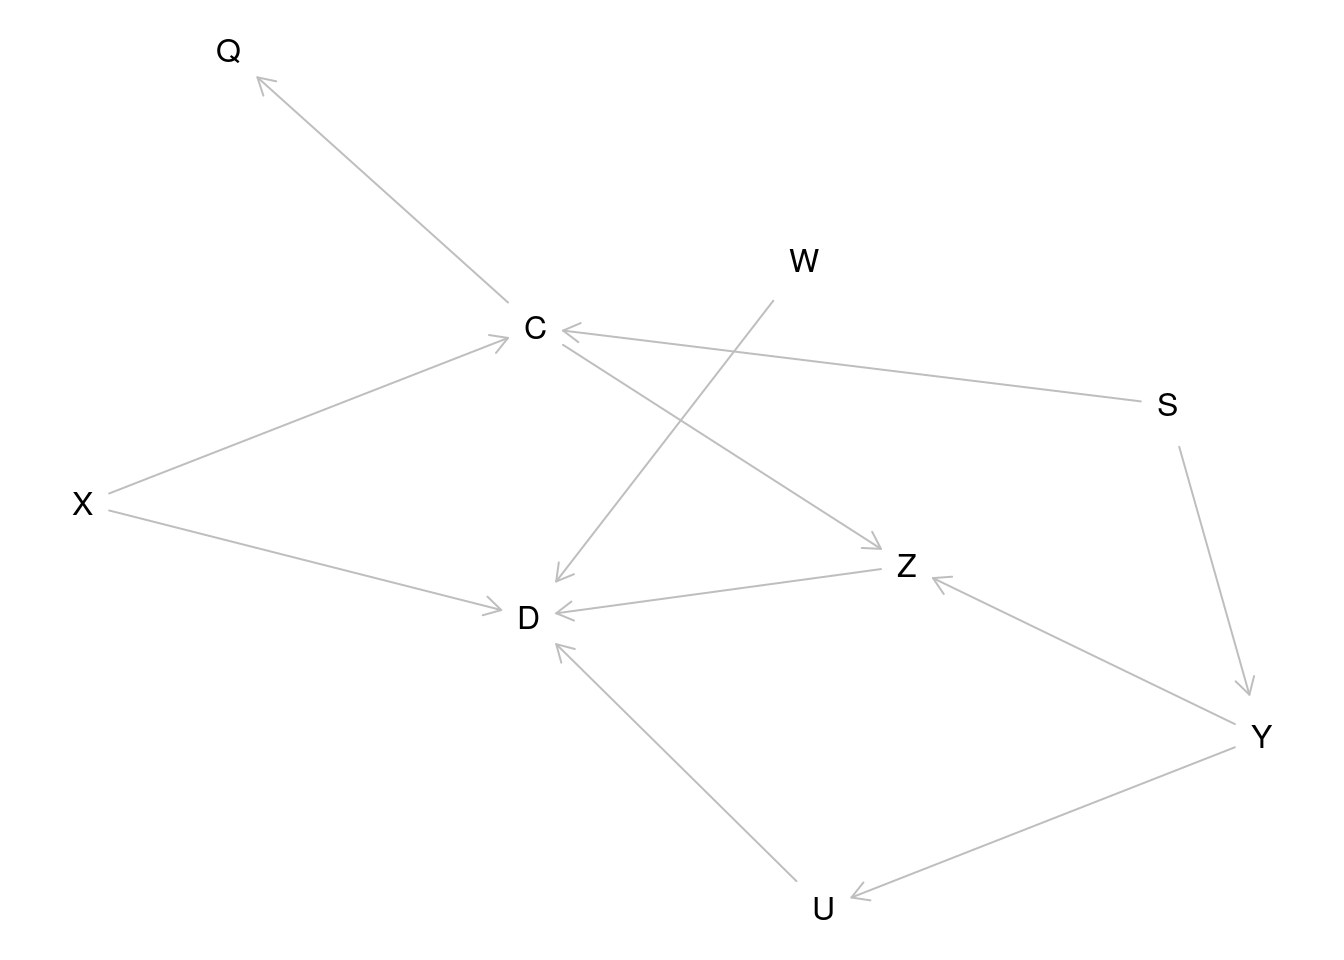
\includegraphics{causal-s_files/figure-latex/dagitty2-1.pdf}

To get a more similar look as on the slide, we must supply the coordinates (x increases from left to right, y from top to bottom):

\begin{Shaded}
\begin{Highlighting}[]
\FunctionTok{coordinates}\NormalTok{(g) }\OtherTok{\textless{}{-}} 
  \FunctionTok{list}\NormalTok{(}
    \AttributeTok{x =} 
      \FunctionTok{c}\NormalTok{(}
        \AttributeTok{S =} \DecValTok{1}\NormalTok{, }\AttributeTok{C =} \DecValTok{1}\NormalTok{, }\AttributeTok{Q =} \DecValTok{1}\NormalTok{, }\AttributeTok{Y =} \DecValTok{2}\NormalTok{, }\AttributeTok{Z =} \DecValTok{2}\NormalTok{, }
        \AttributeTok{X =} \DecValTok{2}\NormalTok{, }\AttributeTok{U =} \DecValTok{3}\NormalTok{, }\AttributeTok{D =} \DecValTok{3}\NormalTok{, }\AttributeTok{W =} \DecValTok{3}
\NormalTok{      ),}
    \AttributeTok{y =} 
      \FunctionTok{c}\NormalTok{(}
        \AttributeTok{U =} \DecValTok{1}\NormalTok{, }\AttributeTok{Y =} \DecValTok{1}\NormalTok{, }\AttributeTok{S =} \DecValTok{1}\NormalTok{, }\AttributeTok{Z =} \DecValTok{2}\NormalTok{, }\AttributeTok{C =} \DecValTok{3}\NormalTok{, }
        \AttributeTok{D =} \DecValTok{3}\NormalTok{, }\AttributeTok{X =} \DecValTok{4}\NormalTok{, }\AttributeTok{W =} \DecValTok{4}\NormalTok{, }\AttributeTok{Q =} \DecValTok{4}
\NormalTok{      )}
\NormalTok{  )}
\FunctionTok{plot}\NormalTok{(g)}
\end{Highlighting}
\end{Shaded}

Let's look at all possible paths from \(C\) to \(D\):

\begin{Shaded}
\begin{Highlighting}[]
\FunctionTok{paths}\NormalTok{(g, }\StringTok{"C"}\NormalTok{, }\StringTok{"D"}\NormalTok{)}\SpecialCharTok{$}\NormalTok{paths}
\end{Highlighting}
\end{Shaded}

As you see, one path contains a collider and is therefore a \emph{closed} path and the others are \emph{open}.

Let's identify the minimal sets of variables needed to adjust the model for \(D\) for, to obtain an unbiased estimate of the effect of \(C\). You can specify, whether you want to estimate direct or total effect of \(C\):

\begin{Shaded}
\begin{Highlighting}[]
\FunctionTok{adjustmentSets}\NormalTok{(}
\NormalTok{  g, }\AttributeTok{exposure =} \StringTok{"C"}\NormalTok{, }\AttributeTok{outcome =} \StringTok{"D"}\NormalTok{, }\AttributeTok{effect =} \StringTok{"direct"}
\NormalTok{)}
\FunctionTok{adjustmentSets}\NormalTok{(}
\NormalTok{  g, }\AttributeTok{exposure =} \StringTok{"C"}\NormalTok{, }\AttributeTok{outcome =} \StringTok{"D"}\NormalTok{, }\AttributeTok{effect =} \StringTok{"total"}
\NormalTok{)}
\end{Highlighting}
\end{Shaded}

Thus, for total effect estimation one should adjust for \(X\) and either \(Y\) or \(S\), whereas for direct effect estimation, one would also need to adjust for \(Z\).

You can verify that, these are the variables that will block all open paths from \(C\) to \(D\).

\textbf{Now try to do the \emph{beer-weight} exercise using \emph{dagitty}: }

\begin{itemize}
\item
  Create the DAG and plot it
\item
  What are the paths from WEIGHT to BEER?
\item
  Will you get the same recommendation for the adjustment variable selection as you found before?
\end{itemize}

\section{Instrumental variables estimation: Mendelian randomization}\label{instrumental-variables-estimation-mendelian-randomization}

Suppose you want to estimate the effect of Body Mass Index (BMI) on blood glucose level (associated with the risk of diabetes).
Let's conduct a simulation study to verify that when the exposure-outcome association is confounded, but there is a valid instrument (genotype), one obtains an unbiased estimate of the causal effect.

\begin{itemize}
\tightlist
\item
  Start by generating the genotype variable as \emph{Binomial(2,p)}, with \(p=0.2\) (and look at the resulting genotype frequencies):
\end{itemize}

\begin{Shaded}
\begin{Highlighting}[]
\NormalTok{n }\OtherTok{\textless{}{-}} \DecValTok{10000}
\NormalTok{mrdat }\OtherTok{\textless{}{-}} \FunctionTok{data.frame}\NormalTok{(}\AttributeTok{G =} \FunctionTok{rbinom}\NormalTok{(n, }\DecValTok{2}\NormalTok{, }\FloatTok{0.2}\NormalTok{))}
\FunctionTok{table}\NormalTok{(mrdat}\SpecialCharTok{$}\NormalTok{G)}
\end{Highlighting}
\end{Shaded}

\begin{itemize}
\tightlist
\item
  Also generate the confounder variable U
\end{itemize}

\begin{Shaded}
\begin{Highlighting}[]
\NormalTok{mrdat}\SpecialCharTok{$}\NormalTok{U }\OtherTok{\textless{}{-}} \FunctionTok{rnorm}\NormalTok{(n)}
\end{Highlighting}
\end{Shaded}

\begin{itemize}
\tightlist
\item
  Generate a continuous (normally distributed) exposure variable \(BMI\) so that it depends on \(G\) and \(U\).
  Check with linear regression, whether there is enough power to get significant parameter estimates.\\
  For instance:
\end{itemize}

\begin{Shaded}
\begin{Highlighting}[]
\NormalTok{mrdat}\SpecialCharTok{$}\NormalTok{BMI }\OtherTok{\textless{}{-}} \FunctionTok{with}\NormalTok{(mrdat, }\DecValTok{25} \SpecialCharTok{+} \FloatTok{0.7} \SpecialCharTok{*}\NormalTok{ G }\SpecialCharTok{+} \DecValTok{2} \SpecialCharTok{*}\NormalTok{ U }\SpecialCharTok{+} \FunctionTok{rnorm}\NormalTok{(n))}
\end{Highlighting}
\end{Shaded}

\begin{itemize}
\tightlist
\item
  Finally generate \(Y\) (``Blood glucose level'') so that it depends on \(BMI\) and \(U\) (but not on \(G\)).
\end{itemize}

\begin{Shaded}
\begin{Highlighting}[]
\NormalTok{mrdat}\SpecialCharTok{$}\NormalTok{Y }\OtherTok{\textless{}{-}} 
  \FunctionTok{with}\NormalTok{(mrdat, }\DecValTok{3} \SpecialCharTok{+} \FloatTok{0.1} \SpecialCharTok{*}\NormalTok{ BMI }\SpecialCharTok{{-}} \FloatTok{1.5} \SpecialCharTok{*}\NormalTok{ U }\SpecialCharTok{+} \FunctionTok{rnorm}\NormalTok{(n, }\DecValTok{0}\NormalTok{, }\FloatTok{0.5}\NormalTok{))}
\end{Highlighting}
\end{Shaded}

\begin{itemize}
\tightlist
\item
  Verify, that simple regression model for \(Y\), with \(BMI\) as a covariate, results in a biased
  estimate of the causal effect (parameter estimate is different from what was generated)
\end{itemize}

How different is the estimate from 0.1?

\begin{itemize}
\item
  Estimate a regression model for \(Y\) with two covariates, \(G\) and \(BMI\). Do you see a significant effect of \(G\)?
  Could you explain analytically, why one may see a significant parameter estimate for \(G\) there?
\item
  Find an IV (instrumental variables) estimate, using G as an instrument, by following the algorithm
  in the lecture notes (use two linear models and find a ratio of the parameter estimates).
  Does the estimate get closer to the generated effect size?
\end{itemize}

\begin{Shaded}
\begin{Highlighting}[]
\NormalTok{mgx }\OtherTok{\textless{}{-}} \FunctionTok{lm}\NormalTok{(BMI }\SpecialCharTok{\textasciitilde{}}\NormalTok{ G, }\AttributeTok{data =}\NormalTok{ mrdat)}
\FunctionTok{ci.lin}\NormalTok{(mgx) }\CommentTok{\# check the instrument effect}
\NormalTok{bgx }\OtherTok{\textless{}{-}}\NormalTok{ mgx}\SpecialCharTok{$}\NormalTok{coef[}\DecValTok{2}\NormalTok{] }\CommentTok{\# save the 2nd coefficient (coef of G)}
\NormalTok{mgy }\OtherTok{\textless{}{-}} \FunctionTok{lm}\NormalTok{(Y }\SpecialCharTok{\textasciitilde{}}\NormalTok{ G, }\AttributeTok{data =}\NormalTok{ mrdat)}
\FunctionTok{ci.lin}\NormalTok{(mgy)}
\NormalTok{bgy }\OtherTok{\textless{}{-}}\NormalTok{ mgy}\SpecialCharTok{$}\NormalTok{coef[}\DecValTok{2}\NormalTok{]}
\NormalTok{causeff }\OtherTok{\textless{}{-}}\NormalTok{ bgy }\SpecialCharTok{/}\NormalTok{ bgx}
\NormalTok{causeff }\CommentTok{\# closer to 0.1?}
\end{Highlighting}
\end{Shaded}

\begin{itemize}
\tightlist
\item
  A proper simulation study would require the analysis to be run several times, to see the extent of variability in the parameter estimates.
  A simple way to do it here would be using a \texttt{for}-loop. Modify the code as follows (exactly the same commands as executed so far, adding a few lines of code to the beginning and to the end):
\end{itemize}

\begin{Shaded}
\begin{Highlighting}[]
\NormalTok{n }\OtherTok{\textless{}{-}} \DecValTok{10000}
\CommentTok{\# initializing simulations:}
\CommentTok{\# 30 simulations (change it, if you want more):}
\NormalTok{nsim }\OtherTok{\textless{}{-}} \DecValTok{30}
\NormalTok{mr }\OtherTok{\textless{}{-}} \FunctionTok{rep}\NormalTok{(}\ConstantTok{NA}\NormalTok{, nsim) }\CommentTok{\# empty vector for the outcome parameters}
\ControlFlowTok{for}\NormalTok{ (i }\ControlFlowTok{in} \DecValTok{1}\SpecialCharTok{:}\NormalTok{nsim) \{ }\CommentTok{\# start the loop}
  \DocumentationTok{\#\# Exactly the same commands as before:}
\NormalTok{  mrdat }\OtherTok{\textless{}{-}} \FunctionTok{data.frame}\NormalTok{(}\AttributeTok{G =} \FunctionTok{rbinom}\NormalTok{(n, }\DecValTok{2}\NormalTok{, }\FloatTok{0.2}\NormalTok{))}
\NormalTok{  mrdat}\SpecialCharTok{$}\NormalTok{U }\OtherTok{\textless{}{-}} \FunctionTok{rnorm}\NormalTok{(n)}
\NormalTok{  mrdat}\SpecialCharTok{$}\NormalTok{BMI }\OtherTok{\textless{}{-}} 
    \FunctionTok{with}\NormalTok{(mrdat, }\DecValTok{25} \SpecialCharTok{+} \FloatTok{0.7} \SpecialCharTok{*}\NormalTok{ G }\SpecialCharTok{+} \DecValTok{2} \SpecialCharTok{*}\NormalTok{ U }\SpecialCharTok{+} \FunctionTok{rnorm}\NormalTok{(n))}
\NormalTok{  mrdat}\SpecialCharTok{$}\NormalTok{Y }\OtherTok{\textless{}{-}} 
    \FunctionTok{with}\NormalTok{(mrdat, }\DecValTok{3} \SpecialCharTok{+} \FloatTok{0.1} \SpecialCharTok{*}\NormalTok{ BMI }\SpecialCharTok{{-}} \FloatTok{1.5} \SpecialCharTok{*}\NormalTok{ U }\SpecialCharTok{+} \FunctionTok{rnorm}\NormalTok{(n, }\DecValTok{0}\NormalTok{, }\FloatTok{0.5}\NormalTok{))}
\NormalTok{  mgx }\OtherTok{\textless{}{-}} \FunctionTok{lm}\NormalTok{(BMI }\SpecialCharTok{\textasciitilde{}}\NormalTok{ G, }\AttributeTok{data =}\NormalTok{ mrdat)}
\NormalTok{  bgx }\OtherTok{\textless{}{-}}\NormalTok{ mgx}\SpecialCharTok{$}\NormalTok{coef[}\DecValTok{2}\NormalTok{]}
\NormalTok{  mgy }\OtherTok{\textless{}{-}} \FunctionTok{lm}\NormalTok{(Y }\SpecialCharTok{\textasciitilde{}}\NormalTok{ G, }\AttributeTok{data =}\NormalTok{ mrdat)}
\NormalTok{  bgy }\OtherTok{\textless{}{-}}\NormalTok{ mgy}\SpecialCharTok{$}\NormalTok{coef[}\DecValTok{2}\NormalTok{]}
  \CommentTok{\# Save the i\textquotesingle{}th parameter estimate:}
\NormalTok{  mr[i] }\OtherTok{\textless{}{-}}\NormalTok{ bgy }\SpecialCharTok{/}\NormalTok{ bgx}
\NormalTok{\} }\CommentTok{\# end the loop}
\end{Highlighting}
\end{Shaded}

Now look at the distribution of the parameter estimate:

\begin{Shaded}
\begin{Highlighting}[]
\FunctionTok{summary}\NormalTok{(mr)}
\end{Highlighting}
\end{Shaded}

\begin{itemize}
\tightlist
\item
  (\emph{optional}) Change the code of simulations so that the assumptions are violated: add a weak direct effect of the genotype G to the equation that generates \(Y\):
\end{itemize}

\begin{Shaded}
\begin{Highlighting}[]
\NormalTok{mrdat}\SpecialCharTok{$}\NormalTok{Y }\OtherTok{\textless{}{-}} 
  \FunctionTok{with}\NormalTok{(}
\NormalTok{    mrdat, }
    \DecValTok{3} \SpecialCharTok{+} \FloatTok{0.1} \SpecialCharTok{*}\NormalTok{ BMI }\SpecialCharTok{{-}} \FloatTok{1.5} \SpecialCharTok{*}\NormalTok{ U }\SpecialCharTok{+} \FloatTok{0.05} \SpecialCharTok{*}\NormalTok{ G }\SpecialCharTok{+} \FunctionTok{rnorm}\NormalTok{(n, }\DecValTok{0}\NormalTok{, }\FloatTok{0.5}\NormalTok{)}
\NormalTok{  )}
\end{Highlighting}
\end{Shaded}

Repeat the simulation study to see, what is the bias in the average estimated causal effect of \(BMI\) on \(Y\).

\begin{itemize}
\tightlist
\item
  (\emph{optional}) Using library \texttt{sem} and function \texttt{tsls}, one can obtain a two-stage least squares estimate for the\\
  causal effect and also the proper standard error. Do you get the same estimate as before?
\end{itemize}

\begin{Shaded}
\begin{Highlighting}[]
\ControlFlowTok{if}\NormalTok{ (}\SpecialCharTok{!}\NormalTok{(}\StringTok{"sem"} \SpecialCharTok{\%in\%} \FunctionTok{installed.packages}\NormalTok{())) }\FunctionTok{install.packages}\NormalTok{(}\StringTok{"sem"}\NormalTok{)}
\FunctionTok{library}\NormalTok{(sem)}
\FunctionTok{summary}\NormalTok{(}\FunctionTok{tsls}\NormalTok{(Y }\SpecialCharTok{\textasciitilde{}}\NormalTok{ BMI, }\SpecialCharTok{\textasciitilde{}}\NormalTok{G, }\AttributeTok{data =}\NormalTok{ mrdat))}
\end{Highlighting}
\end{Shaded}

(There are also several other R packages for IV estimation and Mendelian Randomization (\emph{MendelianRandomization} for instance))

\section{Why are simulation exercises useful for causal inference?}\label{why-are-simulation-exercises-useful-for-causal-inference}

If we simulate the data, we know the data-generating mechanism and the \emph{true} causal effects. So this is a way to check, whether
an analysis approach will lead to estimates that correspond to what is generated. One could expect to see similar phenomena in real
data analysis, if the data-generation mechanism is similar to what was used in simulations.

\chapter{Graphics with ggplot2}\label{graphics-with-ggplot2}

The plot below is from randomized study of the effect of Tamoxifen treatment on bone mineral metabolism in a group of patients who were treated for breast cancer (Kristensen et al, 1994). It is reproduced with permission from the author Peter Dalgaard who has also shared the original data.

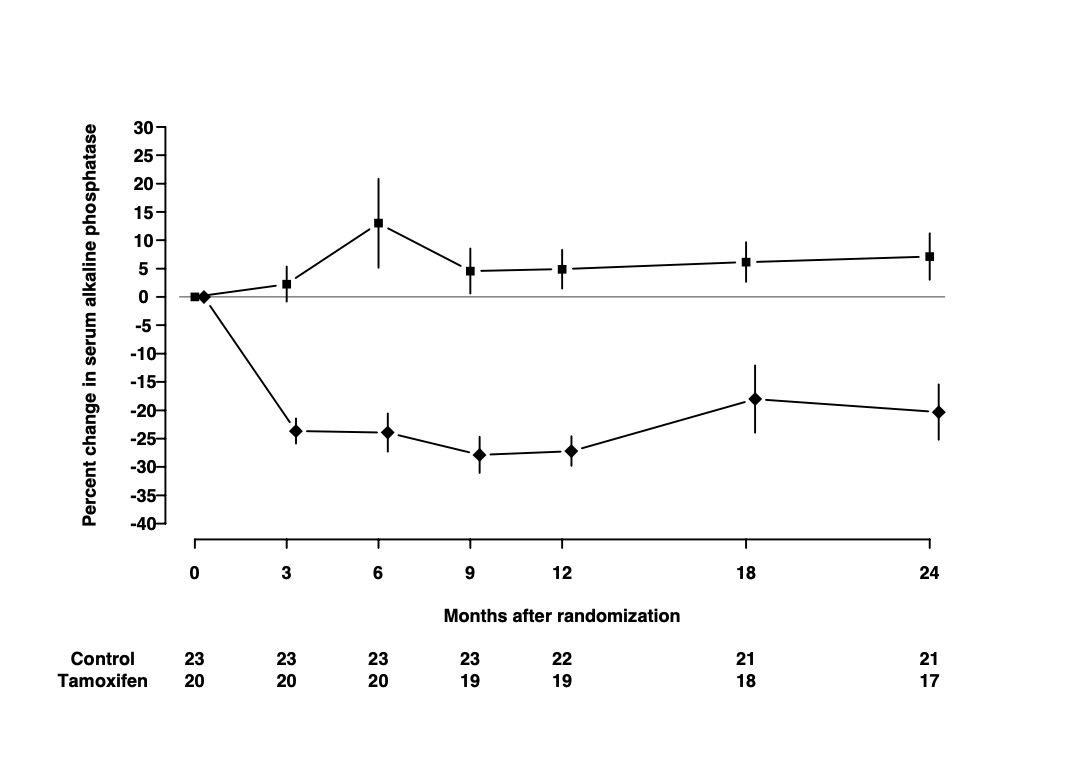
\includegraphics{./graph/bentK.png}

The purpose of this exercise is to show you how to build a similar plot in R using the \texttt{ggplot2} package.

The outcome of the study is the percentage change in serum alkaline phosphate compared with the baseline when the participants first entered the study. The first measurement, on the left of the plot, is zero by definition. Then as we move from left to right, the plot shows the relative changes for the two groups of women: one receiving the anti-cancer drug tamoxifen; the other receiving standard treatment which is referred to as the \emph{control} group. Each woman was randomly allocated to one of these groups on entry to the study. The women returned for follow-up visits until the end of the study at 24 months.

Take a moment to study the graph and try to identify the different graphical elements that we will need to reproduce. Write down a description of these elements and compare it to my summary below.

\begin{itemize}
\tightlist
\item
  The trajectory of the outcome variable is represented by points connected by straight lines. One point represents the mean value for one follow-up visit in one of the groups.
\item
  Separate trajectories are plotted for the treatment and control groups.
\item
  Vertical error bars give a visual impression of the uncertainty associated with each point.
\item
  A horizontal line at zero is drawn as a reference so that we can see the size of the change relative to baseline.
\item
  The x-axis has tick marks at follow-up visits, which are irregularly spaced. Visits occurred every 3 months for the first year, then every 6 months for the second year.
\item
  The y-axis extends beyond the range of the data from -40\% to +30\%.
\item
  A table underneath the x-axis shows the number of women in the treatment and control groups at each visit. These numbers go down as the study progresses. This phenomenon is extremely common in medical studies and is called ``loss to follow-up''.
\end{itemize}

These are the important graphical elements. You may have spotted some other features of the graph, but we will focus on trying to incorporate the features listed above.

\section{Data}\label{data}

The data are available in the file \texttt{alkfos.csv}. This is a text file in comma-separated variable format. It can be read into R using the \texttt{read.csv()} function.

\begin{Shaded}
\begin{Highlighting}[]
\NormalTok{alkfos }\OtherTok{\textless{}{-}} \FunctionTok{read.csv}\NormalTok{(}\StringTok{"./data/alkfos.csv"}\NormalTok{)}
\end{Highlighting}
\end{Shaded}

There are 14 rows in the data frame \texttt{alkfos}: one for each combination of the 7 visits and the 2 groups. The variables in the data frame are:

\begin{itemize}
\tightlist
\item
  \texttt{time} The time since randomization for each follow-up visit.
\item
  \texttt{mean} The outcome variable representing the mean percentage change in serum alkaline phosphate.
\item
  \texttt{available} The number of women still participating in the study.
\item
  \texttt{treat} The treatment group: a character vector taking values ``tamoxifen'' for the treatment group and ``control'' for the control group.
\item
  \texttt{sem} The standard error of the mean used to calculate the length of the error bars.
\end{itemize}

\section{Building the plot}\label{building-the-plot}

\subsection{The ggplot2 package}\label{the-ggplot2-package}

In this exercise, we will be using the R package ggplot2. The ``gg'' stands for ``Grammar of Graphics'', which is a conceptual framework for understanding statistical graphics created by Leland Wilkinson.

The core function in the ggplot2 package is \texttt{ggplot()}. This function requires two arguments:

\begin{itemize}
\tightlist
\item
  \texttt{data} is the name of the data frame that we will take the variables from.
\item
  \texttt{mapping} is the \emph{aesthetic mapping} between variables in the data frame and graphical elements that we want to plot. In this example:

  \begin{itemize}
  \tightlist
  \item
    y-axis is the mean of the percent change in alkaline phosphate represented by the variable \texttt{mean;}
  \item
    x-axis is the visit time represented by the variable \texttt{time.}
  \end{itemize}
\end{itemize}

We make the mapping in a call to the function \texttt{aes()}.

The code below creates a basic plot and assigns it to the object \texttt{p0}.

\begin{Shaded}
\begin{Highlighting}[]
\FunctionTok{library}\NormalTok{(ggplot2, }\AttributeTok{quietly=}\ConstantTok{TRUE}\NormalTok{)}
\NormalTok{p0 }\OtherTok{\textless{}{-}} \FunctionTok{ggplot}\NormalTok{(}\AttributeTok{data=}\NormalTok{alkfos, }\AttributeTok{mapping=}\FunctionTok{aes}\NormalTok{(}\AttributeTok{x=}\NormalTok{time, }\AttributeTok{y=}\NormalTok{mean))}
\end{Highlighting}
\end{Shaded}

Running the code creates the plot but does not display it. This is an important difference between base graphics and ggplot graphics:

\begin{itemize}
\tightlist
\item
  Base graphics functions do not return an R object but will always display a plot on the current graphics device.
\item
  GGplot graphics functions return an R graphical object, which will only be displayed if we ask for it.
\end{itemize}

There are two ways to display a graphical object in R:

\begin{enumerate}
\def\labelenumi{\arabic{enumi}.}
\tightlist
\item
  If we have saved the result to an object, call the \texttt{print()} or \texttt{show()} functions.
\item
  If we have not saved the result, the graphical object will be displayed in the same way that a regular R object is printed to the screen.
\end{enumerate}

The code chunk below displays the object \texttt{p0} created in the chunk above.

\begin{Shaded}
\begin{Highlighting}[]
\FunctionTok{show}\NormalTok{(p0)}
\end{Highlighting}
\end{Shaded}

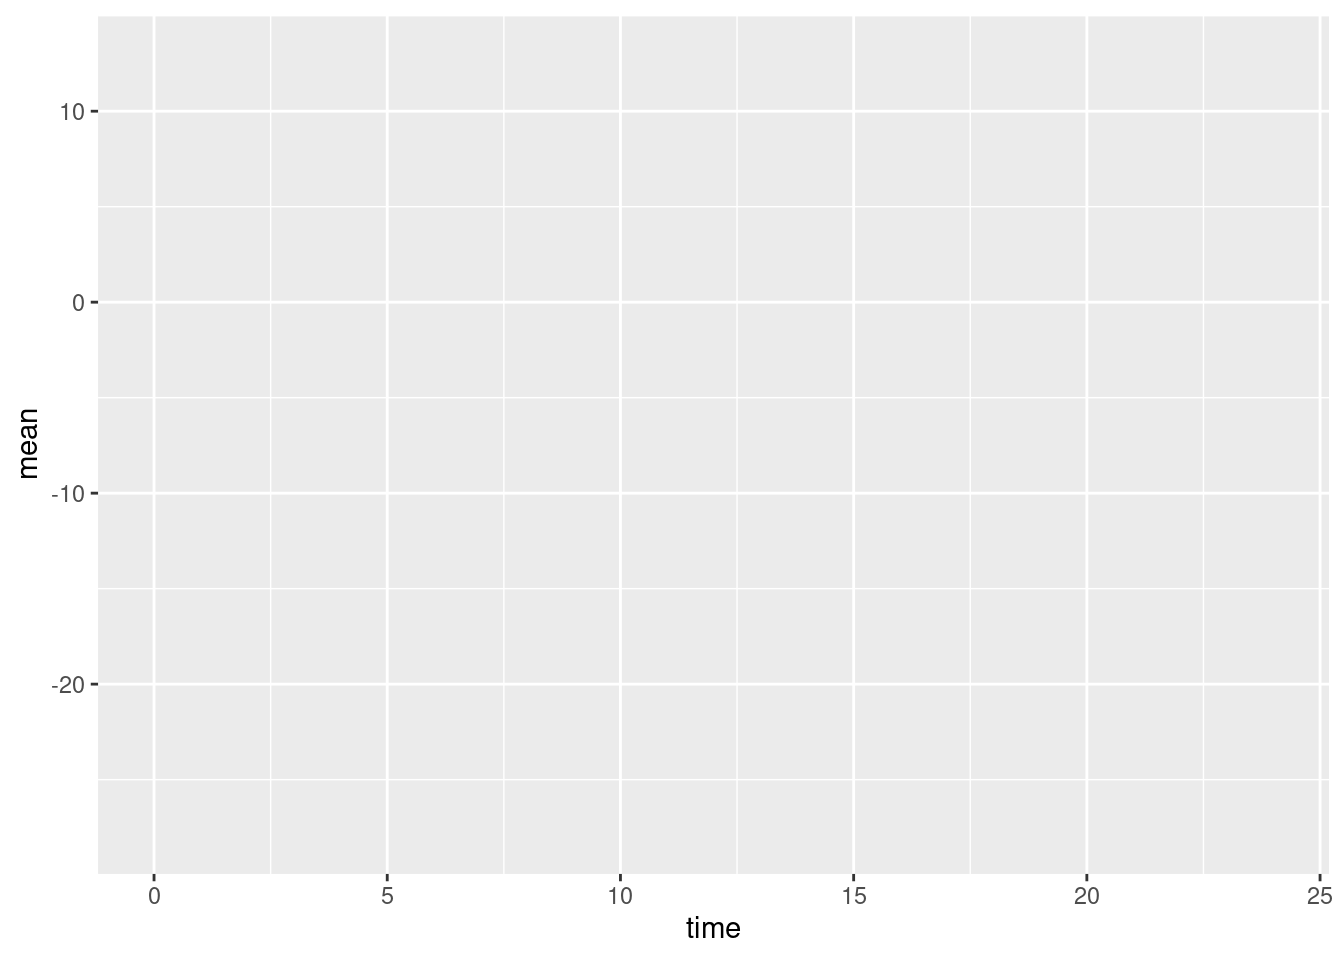
\includegraphics{ggplot2-s_files/figure-latex/unnamed-chunk-4-1.pdf}

You may find the results a little disappointing. The \texttt{ggplot()} function has drawn x- and y-axes that span the range of the data, but otherwise has drawn no points or lines. This is another important difference between ggplot2 and base graphics. Whereas base plotting functions will usually create a sensible default plot, \texttt{ggplot()} makes no assumptions about what you want.

We will recreate the plot in \emph{layers}. Layers are added to a ggplot object by calling additional functions and adding their return value to the basic plot using the \texttt{+} symbol.

\subsection{Geometries}\label{geometries}

The most important layers are \emph{geometries}, which describe how to display the data in the plot. Geometry functions in ggplot2 all start with the prefix \texttt{geom\_}.

\subsubsection{Points and lines}\label{points-and-lines}

We want to plot points representing the mean of the outcome at each visit. This is done with the function \texttt{geom\_point()}. We also want to plot lines between successive points in time. This is done with the function \texttt{geom\_line()}. The code chunk below adds point and line geometries to our basic plot \texttt{p0} and saves the result to the new object \texttt{p1}.

\begin{Shaded}
\begin{Highlighting}[]
\NormalTok{p1 }\OtherTok{\textless{}{-}}\NormalTok{ p0 }\SpecialCharTok{+} \FunctionTok{geom\_point}\NormalTok{() }\SpecialCharTok{+} \FunctionTok{geom\_line}\NormalTok{()}
\FunctionTok{show}\NormalTok{(p1)}
\end{Highlighting}
\end{Shaded}

\includegraphics{ggplot2-s_files/figure-latex/unnamed-chunk-5-1.pdf}

Again, this is not quite what we want. The line geometry is mixing up observations from the treatment and control groups, but we want separate lines for each group. To obtain this we need to add an additional aesthetic mapping inside the call to \texttt{ggplot()}. The aesthetic \texttt{group} gives the name of the variable in the data frame that distinguishes observations from different groups.

Modify the code chunk below so that it includes the \texttt{group} aesthetic to recreate plot \texttt{p1} correctly.

\begin{Shaded}
\begin{Highlighting}[]
\NormalTok{p1 }\OtherTok{\textless{}{-}} \FunctionTok{ggplot}\NormalTok{(}\AttributeTok{data=}\NormalTok{alkfos, }\AttributeTok{mapping=}\FunctionTok{aes}\NormalTok{(}\AttributeTok{x=}\NormalTok{time, }\AttributeTok{y=}\NormalTok{mean)) }\SpecialCharTok{+}
  \FunctionTok{geom\_point}\NormalTok{() }\SpecialCharTok{+} \FunctionTok{geom\_line}\NormalTok{()}
\FunctionTok{show}\NormalTok{(p1)}
\end{Highlighting}
\end{Shaded}

\includegraphics{ggplot2-s_files/figure-latex/unnamed-chunk-6-1.pdf}

\subsubsection{Error bars}\label{error-bars}

Now we can add the error bars. These can be added using the \texttt{linerange} geometry. This geometry needs some new aesthetic mappings. It will inherit the \texttt{x} mapping from the call to \texttt{ggplot()}. However, it needs new mappings \texttt{ymin} and \texttt{ymax} giving the lower and upper points of the error bar on the y-axis. We could go back and modify the aesthetic mappings in the call to \texttt{ggplot()}. However, we can also supply aesthetic mappings inside the call to a geometry function. It can be useful to do this when an aesthetic is only used by one geometry (which is the case here).

Modify the code chunk below so that the \texttt{linerange} geometry has its own aesthetic mapping for \texttt{ymin} and \texttt{ymax}.

\begin{itemize}
\tightlist
\item
  \texttt{ymin} is the mean minus the standard error
\item
  \texttt{ymax} is the mean plus the standard error
\end{itemize}

Note that the error bars are \emph{not confidence intervals}. In statistical graphics it is very common to use plus/minus the standard error to represent the uncertainty in the data without making any statistical claims about coverage.

\begin{Shaded}
\begin{Highlighting}[]
\NormalTok{p2 }\OtherTok{\textless{}{-}}\NormalTok{ p1 }\SpecialCharTok{+} \FunctionTok{geom\_linerange}\NormalTok{(}\AttributeTok{mapping=}\FunctionTok{aes}\NormalTok{(}\AttributeTok{ymin=}\NormalTok{mean}\SpecialCharTok{{-}}\NormalTok{sem, }\AttributeTok{ymax=}\NormalTok{mean}\SpecialCharTok{+}\NormalTok{sem))}
\FunctionTok{show}\NormalTok{(p2)}
\end{Highlighting}
\end{Shaded}

\includegraphics{ggplot2-s_files/figure-latex/unnamed-chunk-7-1.pdf}

Compare the y-axes for plots \texttt{p1} and \texttt{p2}. Note that when we add the error bars, the y-axis automatically expanded the limits of the y-axis to include the highest and lowest values on the error bars.

\subsubsection{Horizontal reference line}\label{horizontal-reference-line}

The last geometry we want to add is the horizontal reference line at zero. This is added using the \texttt{hline} geometry. We must supply the argument \texttt{yintercept} which determines where the horizontal line intersects the y-axis.

We should distinguish the reference line from the lines used to plot the data, otherwise it may distract the viewer. We could do this by changing the colour of the reference line. But here we will use a thinner line using the optional argument \texttt{linewidth} to the hline geometry. The default value of \texttt{linewidth} is 1. A value less than 1 draws a thinner line; a value greater than 1 draws a thicker line. Choose a suitable value for your plot.

\begin{Shaded}
\begin{Highlighting}[]
\NormalTok{p3 }\OtherTok{\textless{}{-}}\NormalTok{ p2 }\SpecialCharTok{+} \FunctionTok{geom\_hline}\NormalTok{(}\AttributeTok{yintercept=}\DecValTok{0}\NormalTok{, }\AttributeTok{linewidth=}\FloatTok{0.1}\NormalTok{)}
\FunctionTok{show}\NormalTok{(p3)}
\end{Highlighting}
\end{Shaded}

\includegraphics{ggplot2-s_files/figure-latex/unnamed-chunk-8-1.pdf}

\subsection{Scales}\label{scales}

Next we want to fix the x- and y-axes. The \texttt{ggplot()} function will provide default axes for you, which are often good enough. But in this case we want custom axes. These are provided by scale functions. In fact axes are just one kind of scale. In the grammar of graphics framework, a scale is a way to annotate any quantity that represents a dimension of the data. This also includes shapes, colours, and sizes.

Both axes are continuous. Therefore we use the \texttt{scale\_x\_continuous()} and \texttt{scale\_y\_continuous()} functions to create custom axes. These scale functions have the same arguments, but they affect the x- and y-axes, respectively. The arguments you want to supply are

\begin{itemize}
\tightlist
\item
  \texttt{breaks} A numeric vector of positions on the axis where you want tick marks.
\item
  \texttt{limits} A numeric vector of length 2 giving the minimum and maximum values to be displayed on the axis.
\end{itemize}

Modify the code chunk below to create the custom axes:

\begin{Shaded}
\begin{Highlighting}[]
\NormalTok{p4 }\OtherTok{\textless{}{-}}\NormalTok{ p3 }\SpecialCharTok{+} \FunctionTok{scale\_x\_continuous}\NormalTok{(}\AttributeTok{breaks=}\FunctionTok{c}\NormalTok{(}\DecValTok{0}\NormalTok{,}\DecValTok{3}\NormalTok{,}\DecValTok{6}\NormalTok{,}\DecValTok{9}\NormalTok{,}\DecValTok{12}\NormalTok{,}\DecValTok{18}\NormalTok{,}\DecValTok{24}\NormalTok{)) }\SpecialCharTok{+}
  \FunctionTok{scale\_y\_continuous}\NormalTok{(}\AttributeTok{breaks=}\FunctionTok{seq}\NormalTok{(}\AttributeTok{from=}\SpecialCharTok{{-}}\DecValTok{40}\NormalTok{, }\AttributeTok{to=}\DecValTok{30}\NormalTok{, }\AttributeTok{by=}\DecValTok{5}\NormalTok{),}
                              \AttributeTok{limits =} \FunctionTok{c}\NormalTok{(}\SpecialCharTok{{-}}\DecValTok{40}\NormalTok{, }\DecValTok{30}\NormalTok{))}
\FunctionTok{show}\NormalTok{(p4)}
\end{Highlighting}
\end{Shaded}

\includegraphics{ggplot2-s_files/figure-latex/unnamed-chunk-9-1.pdf}

We should also supply informative axis labels. The default axis labels are taken from the names of the variables that we used in the aesthetic mappings for \texttt{x} and \texttt{y}. Use the \texttt{xlab()} and \texttt{ylab()} functions to provide informative axis labels.

\begin{Shaded}
\begin{Highlighting}[]
\NormalTok{p5 }\OtherTok{\textless{}{-}}\NormalTok{ p4 }\SpecialCharTok{+} \FunctionTok{xlab}\NormalTok{(}\StringTok{"Months after randomization"}\NormalTok{) }\SpecialCharTok{+} 
  \FunctionTok{ylab}\NormalTok{(}\StringTok{"Percent change in serum alkaline phosphate"}\NormalTok{)}
\FunctionTok{show}\NormalTok{(p5)}
\end{Highlighting}
\end{Shaded}

\includegraphics{ggplot2-s_files/figure-latex/unnamed-chunk-10-1.pdf}

\subsection{Themes}\label{themes}

Our plot contains most of the same graphical elements as the reference plot. But it does not look the same. The original plot was drawn on a white background. But our plot has a grey background with white major and minor grid lines.

Themes control many aspects of the appearance of the plot that do not depend on the data. The default theme, which we have been using so far, is called \texttt{theme\_gray()}. Use the \texttt{help()} function to look up \texttt{theme\_gray()} and you will see the help page documents the other complete themes provided by the ggplot2 package.

\begin{itemize}
\tightlist
\item
  Modify the chunk below to use different themes until you find one that most closely matches the original plot in the file bentK.pdf.
\item
  Find the parameter that changes to the font size and use it to reduce the font until the y-axis label fits.
\end{itemize}

\begin{Shaded}
\begin{Highlighting}[]
\NormalTok{p6 }\OtherTok{\textless{}{-}}\NormalTok{ p5 }\SpecialCharTok{+} \FunctionTok{theme\_classic}\NormalTok{(}\AttributeTok{base\_size=}\DecValTok{9}\NormalTok{)}
\FunctionTok{show}\NormalTok{(p6)}
\end{Highlighting}
\end{Shaded}

\includegraphics{ggplot2-s_files/figure-latex/unnamed-chunk-11-1.pdf}

\subsection{Putting everything together}\label{putting-everything-together}

In this exercise, you have constructed the plot in steps, saving and displaying the plot in separate chunks to allow you to see the changes as we add each layer of the plot. In practice, we do not work like this. All the instructions for creating the plot should be together. Fill in the chunk below so that the plot is recreated in a single chunk.

\begin{Shaded}
\begin{Highlighting}[]
\NormalTok{p }\OtherTok{\textless{}{-}} \FunctionTok{ggplot}\NormalTok{(alkfos, }\AttributeTok{mapping=}\FunctionTok{aes}\NormalTok{(}\AttributeTok{x=}\NormalTok{time, }\AttributeTok{y=}\NormalTok{mean, }\AttributeTok{groups=}\NormalTok{treat)) }\SpecialCharTok{+}
  \FunctionTok{geom\_point}\NormalTok{(}\AttributeTok{mapping=}\FunctionTok{aes}\NormalTok{(}\AttributeTok{shape=}\NormalTok{treat)) }\SpecialCharTok{+}
  \FunctionTok{geom\_line}\NormalTok{() }\SpecialCharTok{+}
  \FunctionTok{geom\_linerange}\NormalTok{(}\AttributeTok{mapping=}\FunctionTok{aes}\NormalTok{(}\AttributeTok{ymin=}\NormalTok{mean}\SpecialCharTok{{-}}\NormalTok{sem, }\AttributeTok{ymax=}\NormalTok{mean}\SpecialCharTok{+}\NormalTok{sem)) }\SpecialCharTok{+}
  \FunctionTok{scale\_x\_continuous}\NormalTok{(}\AttributeTok{breaks=}\FunctionTok{c}\NormalTok{(}\DecValTok{0}\NormalTok{,}\DecValTok{3}\NormalTok{,}\DecValTok{6}\NormalTok{,}\DecValTok{9}\NormalTok{,}\DecValTok{12}\NormalTok{,}\DecValTok{18}\NormalTok{,}\DecValTok{24}\NormalTok{)) }\SpecialCharTok{+}
  \FunctionTok{scale\_y\_continuous}\NormalTok{(}\AttributeTok{breaks=}\FunctionTok{seq}\NormalTok{(}\AttributeTok{from=}\SpecialCharTok{{-}}\DecValTok{40}\NormalTok{, }\AttributeTok{to=}\DecValTok{30}\NormalTok{, }\AttributeTok{by=}\DecValTok{5}\NormalTok{),}
                     \AttributeTok{limits =} \FunctionTok{c}\NormalTok{(}\SpecialCharTok{{-}}\DecValTok{40}\NormalTok{, }\DecValTok{30}\NormalTok{)) }\SpecialCharTok{+}
  \FunctionTok{xlab}\NormalTok{(}\StringTok{"Months after randomization"}\NormalTok{) }\SpecialCharTok{+} 
  \FunctionTok{ylab}\NormalTok{(}\StringTok{"Percent change in serum alkaline phosphate"}\NormalTok{) }\SpecialCharTok{+}
  \FunctionTok{geom\_hline}\NormalTok{(}\AttributeTok{yintercept=}\DecValTok{0}\NormalTok{, }\AttributeTok{linewidth=}\FloatTok{0.1}\NormalTok{) }\SpecialCharTok{+}
  \FunctionTok{theme\_classic}\NormalTok{(}\AttributeTok{base\_size=}\DecValTok{9}\NormalTok{)}
\FunctionTok{show}\NormalTok{(p)}
\end{Highlighting}
\end{Shaded}

\includegraphics{ggplot2-s_files/figure-latex/unnamed-chunk-12-1.pdf}

There is still one thing missing from our reproduction. In the original plot, the treatment and control groups were distinguished by different plotting symbols, whereas in our plot they both have circular marks. We can change this by adding the aesthetic mapping \texttt{shape}.

Modify the chunk above so that the aesthetic \texttt{shape} is mapped onto the variable \texttt{treat}. You can do this inside the call to \texttt{ggplot()} or in the call to \texttt{geom\_point()}.

Note that adding the shape aesthetic automatically adds a legend to the plot, telling us which shape corresponds to which group.

\section{Self study}\label{self-study}

Congratulations, you have mostly recreated the reference figure from Kristensen et al (1994). However, have you really learned anything? The best way to find out is to come back in a week's time and try to recreate the reference plot without looking at this exercise sheet.

You may find it useful to download the ggplot cheatsheet. You can also use R help to find out more about the functions in the ggplot2 package. Finally, you can refer to the book Ggplot2: elegant graphics for data analysis by Hadley Wickham, creator of the ggplot2 package.

\section{Adding the table (advanced topic)}\label{adding-the-table-advanced-topic}

There is one important element missing from the graph. This is the table of the number of participants in each group. This is an advanced topic so instead of explaining each step I am just going to give you the solution. Do not be concerned if you do not understand this part.

Firstly we create a new graphical object to represent the table. This object has its own aesthetic mappings, geometries and scales. I will skip a detailed description of this step except to note that some of the arguments below will suppress graphical features (e.g.~\texttt{NULL} and \texttt{element\_blank()})

\begin{Shaded}
\begin{Highlighting}[]
\NormalTok{tab }\OtherTok{\textless{}{-}} \FunctionTok{ggplot}\NormalTok{(}\AttributeTok{data=}\NormalTok{alkfos, }
              \AttributeTok{mapping=}\FunctionTok{aes}\NormalTok{(}\AttributeTok{x=}\NormalTok{time, }\AttributeTok{y=}\NormalTok{treat, }\AttributeTok{label=}\NormalTok{available)) }\SpecialCharTok{+}
              \FunctionTok{geom\_text}\NormalTok{(}\AttributeTok{size=}\DecValTok{2}\NormalTok{) }\SpecialCharTok{+} \FunctionTok{xlab}\NormalTok{(}\ConstantTok{NULL}\NormalTok{) }\SpecialCharTok{+} \FunctionTok{ylab}\NormalTok{(}\ConstantTok{NULL}\NormalTok{) }\SpecialCharTok{+}
              \FunctionTok{scale\_x\_continuous}\NormalTok{(}\AttributeTok{breaks=}\ConstantTok{NULL}\NormalTok{) }\SpecialCharTok{+} 
              \FunctionTok{theme\_bw}\NormalTok{(}\AttributeTok{base\_size=}\DecValTok{9}\NormalTok{) }\SpecialCharTok{+}
              \FunctionTok{theme}\NormalTok{(}\AttributeTok{panel.grid=}\FunctionTok{element\_blank}\NormalTok{())}
\NormalTok{tab}
\end{Highlighting}
\end{Shaded}

\includegraphics{ggplot2-s_files/figure-latex/unnamed-chunk-13-1.pdf}

Next use the \texttt{plot\_grid()} function from the cowplot package to stack the displayed objects vertically (\texttt{align="v"}), in a single column (\texttt{ncol=1}, \texttt{nrow=2}), with the left and right ends of the x-axes aligned (\texttt{axis="lr"}) and most of the space taken up by the plot (\texttt{rel\_heights=c(5,1)}).

\begin{Shaded}
\begin{Highlighting}[]
\FunctionTok{library}\NormalTok{(cowplot)}
\FunctionTok{plot\_grid}\NormalTok{(}\AttributeTok{plotlist=}\FunctionTok{list}\NormalTok{(p, tab), }\AttributeTok{align=}\StringTok{"v"}\NormalTok{, }\AttributeTok{axis=}\StringTok{"lr"}\NormalTok{, }
          \AttributeTok{ncol=}\DecValTok{1}\NormalTok{, }\AttributeTok{nrow=}\DecValTok{2}\NormalTok{, }\AttributeTok{rel\_heights=}\FunctionTok{c}\NormalTok{(}\DecValTok{5}\NormalTok{,}\DecValTok{1}\NormalTok{))}
\end{Highlighting}
\end{Shaded}

\includegraphics{ggplot2-s_files/figure-latex/unnamed-chunk-14-1.pdf}

\section{References}\label{references}

Kristensen B, Ejlertsen B, Dalgaard P, Larsen L, Holmegaard SN, Transbøl I, Mouridsen HT. Tamoxifen and bone metabolism in postmenopausal low-risk breast cancer patients: a randomized study. \emph{J Clin Oncol}. 1994 May;\textbf{12(5)}:992-7. doi: 10.1200/JCO.1994.12.5.992. PMID: 8164053.

\chapter{Survival analysis with competing risks: Oral cancer patients}\label{survival-analysis-with-competing-risks-oral-cancer-patients}

\section{Description of the data}\label{description-of-the-data}

File \texttt{oralca2.txt}, that you may
access from a url address to be given in the practical, contains data from 338
patients having an oral squamous cell carcinoma diagnosed and treated
in one tertiary level oncological clinic in Finland since 1985, followed-up
for mortality until 31 December 2008.

The dataset contains the following variables:

\begin{longtable}[]{@{}
  >{\raggedright\arraybackslash}p{(\columnwidth - 2\tabcolsep) * \real{0.1231}}
  >{\raggedright\arraybackslash}p{(\columnwidth - 2\tabcolsep) * \real{0.8769}}@{}}
\toprule\noalign{}
\begin{minipage}[b]{\linewidth}\raggedright
Variable
\end{minipage} & \begin{minipage}[b]{\linewidth}\raggedright
Description
\end{minipage} \\
\midrule\noalign{}
\endhead
\bottomrule\noalign{}
\endlastfoot
\texttt{sex} & sex, a factor with categories; \texttt{1\ =\ "Female",\ 2\ =\ "Male"} \\
\texttt{age} & age (years) at the date of diagnosing the cancer \\
\texttt{stage} & TNM stage of the tumour (factor): \texttt{1\ =\ "I",\ ...,\ 4\ =\ "IV",\ 5\ =\ "unkn"} \\
\texttt{time} & follow-up time (in years) since diagnosis until death or censoring \\
\texttt{event} & event ending the follow-up (numeric): \texttt{0\ =\ censoring\ alive,\ 1\ =\ death\ from\ oral\ cancer,\ 2\ =\ death\ from\ other\ causes.} \\
\end{longtable}

\section{Loading the packages and the data}\label{loading-the-packages-and-the-data}

\begin{itemize}
\tightlist
\item
  Load the R packages \texttt{Epi}, and \texttt{survival} needed in this exercise.
\end{itemize}

\begin{Shaded}
\begin{Highlighting}[]
\FunctionTok{library}\NormalTok{(Epi)}
\FunctionTok{library}\NormalTok{(survival)}
\end{Highlighting}
\end{Shaded}

\begin{itemize}
\tightlist
\item
  Read the datafile \texttt{oralca2.txt} from
  a website, whose precise address will be given in the practical,
  into an R data frame named \texttt{orca}.
  Look at the head, structure and the summary of the data frame.
  Using function \texttt{table()} count the numbers of censorings
  as well as deaths from oral cancer and other causes, respectively,
  from the \texttt{event} variable.
\end{itemize}

\begin{Shaded}
\begin{Highlighting}[]
\NormalTok{orca }\OtherTok{\textless{}{-}} \FunctionTok{read.table}\NormalTok{(}\StringTok{"pracs/data/oralca2.txt"}\NormalTok{, }\AttributeTok{header =} \ConstantTok{TRUE}\NormalTok{)}
\FunctionTok{head}\NormalTok{(orca)}
\FunctionTok{str}\NormalTok{(orca)}
\FunctionTok{summary}\NormalTok{(orca)}
\end{Highlighting}
\end{Shaded}

\section{Total mortality: Kaplan--Meier analyses}\label{total-mortality-kaplanmeier-analyses}

\begin{itemize}
\tightlist
\item
  We start our analysis of total mortality pooling the two causes of death into
  a single outcome.
  First, construct a \emph{survival object} \texttt{orca\$suob} from
  the event variable and the follow-up time using function \texttt{Surv()}.
  Look at the structure and summary of \texttt{!orca\$suob!} .
\end{itemize}

\begin{Shaded}
\begin{Highlighting}[]
\NormalTok{orca}\SpecialCharTok{$}\NormalTok{suob }\OtherTok{\textless{}{-}} \FunctionTok{Surv}\NormalTok{(orca}\SpecialCharTok{$}\NormalTok{time, }\DecValTok{1} \SpecialCharTok{*}\NormalTok{ (orca}\SpecialCharTok{$}\NormalTok{event }\SpecialCharTok{\textgreater{}} \DecValTok{0}\NormalTok{))}
\FunctionTok{str}\NormalTok{(orca}\SpecialCharTok{$}\NormalTok{suob)}
\FunctionTok{summary}\NormalTok{(orca}\SpecialCharTok{$}\NormalTok{suob)}
\end{Highlighting}
\end{Shaded}

\begin{itemize}
\tightlist
\item
  Create a \texttt{survfit} object \texttt{s.all}, which does the
  default calculations for a Kaplan--Meier
  analysis of the overall (marginal) survival curve.
\end{itemize}

\begin{Shaded}
\begin{Highlighting}[]
\NormalTok{s.all }\OtherTok{\textless{}{-}} \FunctionTok{survfit}\NormalTok{(suob }\SpecialCharTok{\textasciitilde{}} \DecValTok{1}\NormalTok{, }\AttributeTok{data =}\NormalTok{ orca)}
\end{Highlighting}
\end{Shaded}

See the structure of this object and apply \texttt{print()} method on it, too.
Look at the results; what do you find?
\% Try also \texttt{summary()} and see the outcome.

\begin{Shaded}
\begin{Highlighting}[]
\NormalTok{s.all}
\FunctionTok{str}\NormalTok{(s.all)}
\end{Highlighting}
\end{Shaded}

\begin{itemize}
\tightlist
\item
  The \texttt{summary} method for
  a \texttt{survfit} object would return a lengthy life table.
  However, the \texttt{plot} method with default
  arguments offers the Kaplan--Meier curve
  for a conventional illustration of the survival experience in the whole patient group.
  Alternatively, instead of graphing survival proportions,
  one can draw a curve describing their complements: the cumulative mortality proportions. This curve is drawn together with the survival curve as the
  result of the second command line below.
\end{itemize}

\begin{Shaded}
\begin{Highlighting}[]
\FunctionTok{plot}\NormalTok{(s.all)}
\FunctionTok{lines}\NormalTok{(s.all, }\AttributeTok{fun =} \StringTok{"event"}\NormalTok{, }\AttributeTok{mark.time =}\NormalTok{ F, }\AttributeTok{conf.int =} \ConstantTok{FALSE}\NormalTok{)}
\end{Highlighting}
\end{Shaded}

The effect of option \texttt{mark.time=F} is to omit
marking the times when censorings occurred.

\section{Total mortality by stage}\label{total-mortality-by-stage}

Tumour stage is an important prognostic factor in cancer survival studies.

\begin{itemize}
\tightlist
\item
  Plot separate cumulative mortality curves for the different stage groups
  marking them with different colours, the order which you may define yourself.
  Also find the median survival time for each stage.
\end{itemize}

\begin{Shaded}
\begin{Highlighting}[]
\NormalTok{s.stg }\OtherTok{\textless{}{-}} \FunctionTok{survfit}\NormalTok{(suob }\SpecialCharTok{\textasciitilde{}}\NormalTok{ stage, }\AttributeTok{data =}\NormalTok{ orca)}
\NormalTok{col5 }\OtherTok{\textless{}{-}} \FunctionTok{c}\NormalTok{(}\StringTok{"green"}\NormalTok{, }\StringTok{"blue"}\NormalTok{, }\StringTok{"black"}\NormalTok{, }\StringTok{"red"}\NormalTok{, }\StringTok{"gray"}\NormalTok{)}
\FunctionTok{plot}\NormalTok{(s.stg, }\AttributeTok{col =}\NormalTok{ col5, }\AttributeTok{fun =} \StringTok{"event"}\NormalTok{, }\AttributeTok{mark.time =} \ConstantTok{FALSE}\NormalTok{)}
\NormalTok{s.stg}
\end{Highlighting}
\end{Shaded}

\begin{itemize}
\tightlist
\item
  Create now two parallel plots of which the first one describes the
  cumulative hazards
  and the second one graphs the log-cumulative hazards against log-time
  for the different stages. Compare the two presentations
  with each other and with the one in the previous item.
\end{itemize}

\begin{Shaded}
\begin{Highlighting}[]
\FunctionTok{par}\NormalTok{(}\AttributeTok{mfrow =} \FunctionTok{c}\NormalTok{(}\DecValTok{1}\NormalTok{, }\DecValTok{2}\NormalTok{))}
\FunctionTok{plot}\NormalTok{(s.stg, }\AttributeTok{col =}\NormalTok{ col5, }\AttributeTok{fun =} \StringTok{"cumhaz"}\NormalTok{, }\AttributeTok{main =} \StringTok{"cum. hazards"}\NormalTok{)}
\FunctionTok{plot}\NormalTok{(}
\NormalTok{  s.stg, }
  \AttributeTok{col =}\NormalTok{ col5, }
  \AttributeTok{fun =} \StringTok{"cloglog"}\NormalTok{, }
  \AttributeTok{main =} \StringTok{"cloglog: log cum.haz"}
\NormalTok{)}
\end{Highlighting}
\end{Shaded}

\begin{itemize}
\item
  If the survival times were \emph{exponentially}
  distributed in a given (sub)population
  the corresponding cloglog-curve should follow an approximately linear pattern.
  Could this be the case here in the different stages?
\item
  Also, if the survival distributions of the different subpopulations would
  obey the \emph{proportional hazards} model, the vertical distance between the
  cloglog-curves should be approximately constant over the time axis.
  Do these curves indicate serious deviation from the proportional hazards assumption?
\item
  In the lecture handouts it was observed that
  the crude contrast between males and females in total mortality appears
  unclear, but the age-adjustment in the Cox model provided a more
  expected hazard ratio estimate.
  We shall examine the confounding by age somewhat closer.
  First categorize the continuous age variable
  into, say, three categories by function \texttt{cut()}
  using suitable breakpoints, like 55 and 75 years, and
  cross-tabulate sex and age group:
\end{itemize}

\begin{Shaded}
\begin{Highlighting}[]
\NormalTok{orca}\SpecialCharTok{$}\NormalTok{agegr }\OtherTok{\textless{}{-}} \FunctionTok{cut}\NormalTok{(orca}\SpecialCharTok{$}\NormalTok{age, }\AttributeTok{br =} \FunctionTok{c}\NormalTok{(}\DecValTok{0}\NormalTok{, }\DecValTok{55}\NormalTok{, }\DecValTok{75}\NormalTok{, }\DecValTok{95}\NormalTok{))}
\FunctionTok{stat.table}\NormalTok{(}\FunctionTok{list}\NormalTok{(sex, agegr), }\FunctionTok{list}\NormalTok{(}\FunctionTok{count}\NormalTok{(), }\FunctionTok{percent}\NormalTok{(agegr)),}
  \AttributeTok{margins =} \ConstantTok{TRUE}\NormalTok{, }
  \AttributeTok{data =}\NormalTok{ orca}
\NormalTok{)}
\end{Highlighting}
\end{Shaded}

Male patients are clearly younger than females in these data.

Now, plot Kaplan--Meier curves jointly classified by sex and age.

\begin{Shaded}
\begin{Highlighting}[]
\NormalTok{s.agrx }\OtherTok{\textless{}{-}} \FunctionTok{survfit}\NormalTok{(suob }\SpecialCharTok{\textasciitilde{}}\NormalTok{ agegr }\SpecialCharTok{+}\NormalTok{ sex, }\AttributeTok{data =}\NormalTok{ orca)}
\FunctionTok{par}\NormalTok{(}\AttributeTok{mfrow =} \FunctionTok{c}\NormalTok{(}\DecValTok{1}\NormalTok{, }\DecValTok{1}\NormalTok{))}
\FunctionTok{plot}\NormalTok{(s.agrx,}
  \AttributeTok{fun =} \StringTok{"event"}\NormalTok{, }\AttributeTok{mark.time =} \ConstantTok{FALSE}\NormalTok{, }\AttributeTok{xlim =} \FunctionTok{c}\NormalTok{(}\DecValTok{0}\NormalTok{, }\DecValTok{15}\NormalTok{),}
  \AttributeTok{col =} \FunctionTok{rep}\NormalTok{(}\FunctionTok{c}\NormalTok{(}\StringTok{"red"}\NormalTok{, }\StringTok{"blue"}\NormalTok{), }\DecValTok{3}\NormalTok{), }\AttributeTok{lty =} \FunctionTok{c}\NormalTok{(}\DecValTok{2}\NormalTok{, }\DecValTok{2}\NormalTok{, }\DecValTok{1}\NormalTok{, }\DecValTok{1}\NormalTok{, }\DecValTok{5}\NormalTok{, }\DecValTok{5}\NormalTok{)}
\NormalTok{)}
\end{Highlighting}
\end{Shaded}

In each age band the mortality curve for males is on a higher level
than that for females.

\section{Event-specific cumulative mortality curves}\label{event-specific-cumulative-mortality-curves}

We move on to analysing cumulative mortalities for the
two causes of death separately, first overall and then
by prognostic factors.

\begin{itemize}
\tightlist
\item
  Use the \texttt{survfit}-function in \texttt{survival} package with option \texttt{type="mstate"}.
\end{itemize}

\begin{Shaded}
\begin{Highlighting}[]
\FunctionTok{library}\NormalTok{(survival)}
\NormalTok{cif1 }\OtherTok{\textless{}{-}} \FunctionTok{survfit}\NormalTok{(}\FunctionTok{Surv}\NormalTok{(time, event, }\AttributeTok{type =} \StringTok{"mstate"}\NormalTok{) }\SpecialCharTok{\textasciitilde{}} \DecValTok{1}\NormalTok{,}
  \AttributeTok{data =}\NormalTok{ orca}
\NormalTok{)}
\FunctionTok{str}\NormalTok{(cif1)}
\end{Highlighting}
\end{Shaded}

\begin{itemize}
\tightlist
\item
  One could apply here the plot method of the survfit object to plot the
  cumulative incidences for each cause. However, we suggest that you use
  instead a simple function \texttt{plotCIF()} found in the \texttt{Epi} package.
  The main arguments are
\end{itemize}

\begin{longtable}[]{@{}ll@{}}
\toprule\noalign{}
\endhead
\bottomrule\noalign{}
\endlastfoot
\texttt{data} & data frame created by function \}\texttt{survfit()} \\
\texttt{event} & indicator for the event: values 1 or 2. \\
\end{longtable}

Other arguments are like in the ordinary \texttt{plot()} function.

\begin{itemize}
\tightlist
\item
  Draw two parallel plots describing
  the overall cumulative incidence curves for both causes of death
\end{itemize}

\begin{Shaded}
\begin{Highlighting}[]
\FunctionTok{par}\NormalTok{(}\AttributeTok{mfrow =} \FunctionTok{c}\NormalTok{(}\DecValTok{1}\NormalTok{, }\DecValTok{2}\NormalTok{))}
\FunctionTok{plotCIF}\NormalTok{(cif1, }\DecValTok{1}\NormalTok{, }\AttributeTok{main =} \StringTok{"Cancer death"}\NormalTok{)}
\FunctionTok{plotCIF}\NormalTok{(cif1, }\DecValTok{2}\NormalTok{, }\AttributeTok{main =} \StringTok{"Other deaths"}\NormalTok{)}
\end{Highlighting}
\end{Shaded}

\begin{itemize}
\tightlist
\item
  Compute the estimated
  cumulative incidences by stage for both causes of death.
  Now you have to add variable \texttt{stage} to survfit-function.
\end{itemize}

See the structure of the resulting object, in which you should
observe strata variable containing the stage grouping variable. Plot the pertinent curves in two parallel graphs.
Cut the \(y\)-axis for a more efficient graphical presentation

\begin{Shaded}
\begin{Highlighting}[]
\NormalTok{col5 }\OtherTok{\textless{}{-}} \FunctionTok{c}\NormalTok{(}\StringTok{"green"}\NormalTok{, }\StringTok{"blue"}\NormalTok{, }\StringTok{"black"}\NormalTok{, }\StringTok{"red"}\NormalTok{, }\StringTok{"gray"}\NormalTok{)}
\NormalTok{cif2 }\OtherTok{\textless{}{-}} \FunctionTok{survfit}\NormalTok{(}\FunctionTok{Surv}\NormalTok{(time, event, }\AttributeTok{type =} \StringTok{"mstate"}\NormalTok{) }\SpecialCharTok{\textasciitilde{}}\NormalTok{ stage,}
  \AttributeTok{data =}\NormalTok{ orca}
\NormalTok{)}
\FunctionTok{str}\NormalTok{(cif2)}

\FunctionTok{par}\NormalTok{(}\AttributeTok{mfrow =} \FunctionTok{c}\NormalTok{(}\DecValTok{1}\NormalTok{, }\DecValTok{2}\NormalTok{))}
\FunctionTok{plotCIF}\NormalTok{(cif2, }\DecValTok{1}\NormalTok{,}
  \AttributeTok{main =} \StringTok{"Cancer death by stage"}\NormalTok{,}
  \AttributeTok{col =}\NormalTok{ col5, }\AttributeTok{ylim =} \FunctionTok{c}\NormalTok{(}\DecValTok{0}\NormalTok{, }\FloatTok{0.7}\NormalTok{)}
\NormalTok{)}
\FunctionTok{plotCIF}\NormalTok{(cif2, }\DecValTok{2}\NormalTok{,}
  \AttributeTok{main =} \StringTok{"Other deaths by stage"}\NormalTok{,}
  \AttributeTok{col =}\NormalTok{ col5, }\AttributeTok{ylim =} \FunctionTok{c}\NormalTok{(}\DecValTok{0}\NormalTok{, }\FloatTok{0.7}\NormalTok{)}
\NormalTok{)}
\end{Highlighting}
\end{Shaded}

Compare the two plots. What would you conclude about the
effect of stage on the two causes of death?

\begin{itemize}
\tightlist
\item
  Using another function \texttt{stackedCIF()} in \texttt{Epi} you can
  put the two cumulative incidence curves in one graph but stacked upon one another such that
  the lower curve is for the cancer deaths and the upper curve is for total mortality,
  and the vertical difference between the two curves describes the
  cumulative mortality from other causes. You can also add some colours for the different zones:
\end{itemize}

\begin{Shaded}
\begin{Highlighting}[]
\FunctionTok{par}\NormalTok{(}\AttributeTok{mfrow =} \FunctionTok{c}\NormalTok{(}\DecValTok{1}\NormalTok{, }\DecValTok{1}\NormalTok{))}
\FunctionTok{stackedCIF}\NormalTok{(cif1, }\AttributeTok{colour =} \FunctionTok{c}\NormalTok{(}\StringTok{"gray70"}\NormalTok{, }\StringTok{"gray85"}\NormalTok{))}
\end{Highlighting}
\end{Shaded}

\section{Regression modelling of overall mortality.}\label{regression-modelling-of-overall-mortality.}

\begin{itemize}
\tightlist
\item
  Fit the semiparametric proportional hazards
  regression model, a.k.a. the Cox model, on all deaths including
  sex, age and stage as covariates. Use function
  \texttt{coxph()} in package \texttt{survival}.
  It is often useful to center and scale
  continuous covariates like \texttt{age} here.
  The estimated rate ratios and their confidence intervals
  can also here be displayed by applying \texttt{ci.lin()}
  on the fitted model object.
\end{itemize}

\begin{Shaded}
\begin{Highlighting}[]
\FunctionTok{options}\NormalTok{(}\AttributeTok{show.signif.stars =} \ConstantTok{FALSE}\NormalTok{)}
\NormalTok{m1 }\OtherTok{\textless{}{-}} \FunctionTok{coxph}\NormalTok{(suob }\SpecialCharTok{\textasciitilde{}}\NormalTok{ sex }\SpecialCharTok{+} \FunctionTok{I}\NormalTok{((age }\SpecialCharTok{{-}} \DecValTok{65}\NormalTok{) }\SpecialCharTok{/} \DecValTok{10}\NormalTok{) }\SpecialCharTok{+}\NormalTok{ stage, }\AttributeTok{data =}\NormalTok{ orca)}
\FunctionTok{summary}\NormalTok{(m1)}
\FunctionTok{round}\NormalTok{(}\FunctionTok{ci.exp}\NormalTok{(m1), }\DecValTok{4}\NormalTok{)}
\end{Highlighting}
\end{Shaded}

Look at the results. What are the main findings?

\begin{itemize}
\tightlist
\item
  Check whether the data are sufficiently consistent with the
  assumption of proportional hazards with respect to each of
  the variables separately
  as well as globally, using the \texttt{cox.zph()} function.
\end{itemize}

\begin{Shaded}
\begin{Highlighting}[]
\FunctionTok{cox.zph}\NormalTok{(m1)}
\end{Highlighting}
\end{Shaded}

\begin{itemize}
\tightlist
\item
  No evidence against proportionality assumption could apparently be found.
  Moreover, no difference can be observed between stages I and II in the estimates.
  On the other hand, the
  group with stage unknown is a complex mixture of patients from various
  true stages. Therefore, it may be prudent to exclude these subjects from the data
  and to pool the first two stage groups into one. After that fit a model in
  the reduced data with the new stage variable.
\end{itemize}

\begin{Shaded}
\begin{Highlighting}[]
\NormalTok{orca2 }\OtherTok{\textless{}{-}} \FunctionTok{subset}\NormalTok{(orca, stage }\SpecialCharTok{!=} \StringTok{"unkn"}\NormalTok{)}
\NormalTok{orca2}\SpecialCharTok{$}\NormalTok{st3 }\OtherTok{\textless{}{-}} \FunctionTok{Relevel}\NormalTok{(orca2}\SpecialCharTok{$}\NormalTok{stage, }\FunctionTok{list}\NormalTok{(}\DecValTok{1}\SpecialCharTok{:}\DecValTok{2}\NormalTok{, }\DecValTok{3}\NormalTok{, }\DecValTok{4}\SpecialCharTok{:}\DecValTok{5}\NormalTok{))}
\FunctionTok{levels}\NormalTok{(orca2}\SpecialCharTok{$}\NormalTok{st3) }\OtherTok{\textless{}{-}} \FunctionTok{c}\NormalTok{(}\StringTok{"I{-}II"}\NormalTok{, }\StringTok{"III"}\NormalTok{, }\StringTok{"IV"}\NormalTok{)}
\NormalTok{m2 }\OtherTok{\textless{}{-}} \FunctionTok{update}\NormalTok{(m1, . }\SpecialCharTok{\textasciitilde{}}\NormalTok{ . }\SpecialCharTok{{-}}\NormalTok{ stage }\SpecialCharTok{+}\NormalTok{ st3, }\AttributeTok{data =}\NormalTok{ orca2)}
\FunctionTok{round}\NormalTok{(}\FunctionTok{ci.exp}\NormalTok{(m2), }\DecValTok{4}\NormalTok{)}
\end{Highlighting}
\end{Shaded}

\begin{itemize}
\tightlist
\item
  Plot the predicted cumulative mortality curves by stage,
  jointly stratified by sex and age, focusing
  only on 40 and 80 year old patients, respectively,
  based on the fitted model \texttt{m2}.
  You need to create a new artificial data frame
  containing the desired values for the covariates.
\end{itemize}

\begin{Shaded}
\begin{Highlighting}[]
\NormalTok{newd }\OtherTok{\textless{}{-}} \FunctionTok{data.frame}\NormalTok{(}
  \AttributeTok{sex =} \FunctionTok{c}\NormalTok{(}\FunctionTok{rep}\NormalTok{(}\StringTok{"Male"}\NormalTok{, }\DecValTok{6}\NormalTok{), }\FunctionTok{rep}\NormalTok{(}\StringTok{"Female"}\NormalTok{, }\DecValTok{6}\NormalTok{)),}
  \AttributeTok{age =} \FunctionTok{rep}\NormalTok{(}\FunctionTok{c}\NormalTok{(}\FunctionTok{rep}\NormalTok{(}\DecValTok{40}\NormalTok{, }\DecValTok{3}\NormalTok{), }\FunctionTok{rep}\NormalTok{(}\DecValTok{80}\NormalTok{, }\DecValTok{3}\NormalTok{)), }\DecValTok{2}\NormalTok{),}
  \AttributeTok{st3 =} \FunctionTok{rep}\NormalTok{(}\FunctionTok{levels}\NormalTok{(orca2}\SpecialCharTok{$}\NormalTok{st3), }\DecValTok{4}\NormalTok{)}
\NormalTok{)}
\NormalTok{newd}
\NormalTok{col3 }\OtherTok{\textless{}{-}} \FunctionTok{c}\NormalTok{(}\StringTok{"green"}\NormalTok{, }\StringTok{"black"}\NormalTok{, }\StringTok{"red"}\NormalTok{)}
\FunctionTok{par}\NormalTok{(}\AttributeTok{mfrow =} \FunctionTok{c}\NormalTok{(}\DecValTok{1}\NormalTok{, }\DecValTok{2}\NormalTok{))}
\FunctionTok{plot}\NormalTok{(}
  \FunctionTok{survfit}\NormalTok{(}
\NormalTok{    m2, }\AttributeTok{newdata =} \FunctionTok{subset}\NormalTok{(newd, sex }\SpecialCharTok{==} \StringTok{"Male"} \SpecialCharTok{\&}\NormalTok{ age }\SpecialCharTok{==} \DecValTok{40}\NormalTok{)}
\NormalTok{  ),}
  \AttributeTok{col =}\NormalTok{ col3, }\AttributeTok{fun =} \StringTok{"event"}\NormalTok{, }\AttributeTok{mark.time =} \ConstantTok{FALSE}
\NormalTok{)}
\FunctionTok{lines}\NormalTok{(}
  \FunctionTok{survfit}\NormalTok{(}
\NormalTok{    m2, }\AttributeTok{newdata =} \FunctionTok{subset}\NormalTok{(newd, sex }\SpecialCharTok{==} \StringTok{"Female"} \SpecialCharTok{\&}\NormalTok{ age }\SpecialCharTok{==} \DecValTok{40}\NormalTok{)}
\NormalTok{  ),}
  \AttributeTok{col =}\NormalTok{ col3, }\AttributeTok{fun =} \StringTok{"event"}\NormalTok{, }\AttributeTok{lty =} \DecValTok{2}\NormalTok{, }\AttributeTok{mark.time =} \ConstantTok{FALSE}
\NormalTok{)}
\FunctionTok{plot}\NormalTok{(}
  \FunctionTok{survfit}\NormalTok{(}
\NormalTok{    m2, }\AttributeTok{newdata =} \FunctionTok{subset}\NormalTok{(newd, sex }\SpecialCharTok{==} \StringTok{"Male"} \SpecialCharTok{\&}\NormalTok{ age }\SpecialCharTok{==} \DecValTok{80}\NormalTok{)}
\NormalTok{  ),}
  \AttributeTok{ylim =} \FunctionTok{c}\NormalTok{(}\DecValTok{0}\NormalTok{, }\DecValTok{1}\NormalTok{), }\AttributeTok{col =}\NormalTok{ col3, }\AttributeTok{fun =} \StringTok{"event"}\NormalTok{, }\AttributeTok{mark.time =} \ConstantTok{FALSE}
\NormalTok{)}
\FunctionTok{lines}\NormalTok{(}
  \FunctionTok{survfit}\NormalTok{(}
\NormalTok{    m2, }\AttributeTok{newdata =} \FunctionTok{subset}\NormalTok{(newd, sex }\SpecialCharTok{==} \StringTok{"Female"} \SpecialCharTok{\&}\NormalTok{ age }\SpecialCharTok{==} \DecValTok{80}\NormalTok{)}
\NormalTok{  ),}
  \AttributeTok{col =}\NormalTok{ col3, }\AttributeTok{fun =} \StringTok{"event"}\NormalTok{, }\AttributeTok{lty =} \DecValTok{2}\NormalTok{, }\AttributeTok{mark.time =} \ConstantTok{FALSE}
\NormalTok{)}
\end{Highlighting}
\end{Shaded}

\section{Modelling event-specific hazards}\label{modelling-event-specific-hazards}

\begin{itemize}
\tightlist
\item
  Fit the Cox model for the cause-specific hazard of cancer deaths
  with the same covariates as above. In this case
  only cancer deaths are counted as events and deaths from other causes
  are included into censorings.
\end{itemize}

\begin{Shaded}
\begin{Highlighting}[]
\NormalTok{m2haz1 }\OtherTok{\textless{}{-}} 
  \FunctionTok{coxph}\NormalTok{(}
    \FunctionTok{Surv}\NormalTok{(time, event }\SpecialCharTok{==} \DecValTok{1}\NormalTok{) }\SpecialCharTok{\textasciitilde{}}\NormalTok{ sex }\SpecialCharTok{+} \FunctionTok{I}\NormalTok{((age }\SpecialCharTok{{-}} \DecValTok{65}\NormalTok{) }\SpecialCharTok{/} \DecValTok{10}\NormalTok{) }\SpecialCharTok{+}\NormalTok{ st3, }
    \AttributeTok{data =}\NormalTok{ orca2}
\NormalTok{  )}
\FunctionTok{round}\NormalTok{(}\FunctionTok{ci.exp}\NormalTok{(m2haz1), }\DecValTok{4}\NormalTok{)}
\FunctionTok{cox.zph}\NormalTok{(m2haz1)}
\end{Highlighting}
\end{Shaded}

Compare the results with those of model \texttt{m2}. What are the major differences?

\begin{itemize}
\tightlist
\item
  Fit a similar model for deaths from other causes and compare the results.
\end{itemize}

\begin{Shaded}
\begin{Highlighting}[]
\NormalTok{m2haz2 }\OtherTok{\textless{}{-}} 
  \FunctionTok{coxph}\NormalTok{(}
    \FunctionTok{Surv}\NormalTok{(time, event }\SpecialCharTok{==} \DecValTok{2}\NormalTok{) }\SpecialCharTok{\textasciitilde{}}\NormalTok{ sex }\SpecialCharTok{+} \FunctionTok{I}\NormalTok{((age }\SpecialCharTok{{-}} \DecValTok{65}\NormalTok{) }\SpecialCharTok{/} \DecValTok{10}\NormalTok{) }\SpecialCharTok{+}\NormalTok{ st3, }
    \AttributeTok{data =}\NormalTok{ orca2}
\NormalTok{  )}
\FunctionTok{round}\NormalTok{(}\FunctionTok{ci.exp}\NormalTok{(m2haz2), }\DecValTok{4}\NormalTok{)}
\FunctionTok{cox.zph}\NormalTok{(m2haz2)}
\end{Highlighting}
\end{Shaded}

\section{Lexis object with multi-state set-up}\label{lexis-object-with-multi-state-set-up}

Before entering to multi-state analyses, it might be instructive to apply some Lexis tools to illustrate the competing-risks set-up.
More detailed explanation of these tools will be given by Bendix later.

\begin{itemize}
\tightlist
\item
  Form a \texttt{Lexis} object from the data frame and
  print a summary of it. We shall name the main (and only) time axis
  in this object as \texttt{stime}.
\end{itemize}

\begin{Shaded}
\begin{Highlighting}[]
\NormalTok{orca.lex }\OtherTok{\textless{}{-}} \FunctionTok{Lexis}\NormalTok{(}
  \AttributeTok{exit =} \FunctionTok{list}\NormalTok{(}\AttributeTok{stime =}\NormalTok{ time),}
  \AttributeTok{exit.status =} \FunctionTok{factor}\NormalTok{(event,}
    \AttributeTok{labels =} \FunctionTok{c}\NormalTok{(}\StringTok{"Alive"}\NormalTok{, }\StringTok{"Oral ca. death"}\NormalTok{, }\StringTok{"Other death"}\NormalTok{)}
\NormalTok{  ),}
  \AttributeTok{data =}\NormalTok{ orca}
\NormalTok{)}
\FunctionTok{summary}\NormalTok{(orca.lex)}
\end{Highlighting}
\end{Shaded}

\begin{itemize}
\tightlist
\item
  Draw a box diagram of the two-state set-up of competing transitions. Run first th e following command line
\end{itemize}

\begin{Shaded}
\begin{Highlighting}[]
\FunctionTok{boxes}\NormalTok{(orca.lex)}
\end{Highlighting}
\end{Shaded}

Now, move the cursor to the point in the graphics window, at which you wish to put the box for \emph{Alive}, and click. Next, move
the cursor to the point at which you wish to have the box for \emph{Oral ca. death}, and click. Finally, do the same with the box for \emph{Other death}.
If you are not happy with the outcome, run the command line again and repeat the necessary mouse moves and clicks.

\section{Optional: Poisson regression as an alternative to Cox model}\label{optional-poisson-regression-as-an-alternative-to-cox-model}

It can be shown that the Cox model with an unspecified form for the
baseline hazard \(\lambda_0(t)\) is mathematically equivalent
to the following kind of Poisson regression model.
Time is treated as a categorical factor with
a dense division of the time axis
into disjoint intervals or \emph{timebands} such that
only one outcome event occurs in each timeband.
The model formula contains this time factor plus the desired
explanatory terms.

A sufficient division of time axis is obtained by
first setting the break points
between adjacent timebands to be those time points at which an outcome event has been observed to occur. Then,
the pertinent \texttt{lexis} object is created
and after that it will be split according to those breakpoints.
Finally, the Poisson regression model is fitted
on the splitted \texttt{lexis} object using function \texttt{glm()} with appropriate specifications.

We shall now demonstrate the numerical equivalence of the Cox model
\texttt{m2haz1} for oral cancer mortality that was fitted above,
and the corresponding Poisson regression.

\begin{itemize}
\tightlist
\item
  First we form the necessary \texttt{lexis} object by just taking
  the relevant subset of the already available \texttt{orca.lex} object.
  Upon that the three-level stage factor \texttt{st3} is created
  as above.
\end{itemize}

\begin{Shaded}
\begin{Highlighting}[]
\NormalTok{orca2.lex }\OtherTok{\textless{}{-}} \FunctionTok{subset}\NormalTok{(orca.lex, stage }\SpecialCharTok{!=} \StringTok{"unkn"}\NormalTok{)}
\NormalTok{orca2.lex}\SpecialCharTok{$}\NormalTok{st3 }\OtherTok{\textless{}{-}} \FunctionTok{Relevel}\NormalTok{(orca2}\SpecialCharTok{$}\NormalTok{stage, }\FunctionTok{list}\NormalTok{(}\DecValTok{1}\SpecialCharTok{:}\DecValTok{2}\NormalTok{, }\DecValTok{3}\NormalTok{, }\DecValTok{4}\SpecialCharTok{:}\DecValTok{5}\NormalTok{))}
\FunctionTok{levels}\NormalTok{(orca2.lex}\SpecialCharTok{$}\NormalTok{st3) }\OtherTok{\textless{}{-}} \FunctionTok{c}\NormalTok{(}\StringTok{"I{-}II"}\NormalTok{, }\StringTok{"III"}\NormalTok{, }\StringTok{"IV"}\NormalTok{)}
\end{Highlighting}
\end{Shaded}

Then, the break points of time axis are taken from
the sorted event times, and the \texttt{lexis} object is
split by those breakpoints. The \texttt{timeband} factor
is defined according to the splitted survival times
stored in variable \texttt{stime}.

\begin{Shaded}
\begin{Highlighting}[]
\NormalTok{cuts }\OtherTok{\textless{}{-}} \FunctionTok{sort}\NormalTok{(orca2}\SpecialCharTok{$}\NormalTok{time[orca2}\SpecialCharTok{$}\NormalTok{event }\SpecialCharTok{==} \DecValTok{1}\NormalTok{])}
\NormalTok{orca2.spl }\OtherTok{\textless{}{-}} 
  \FunctionTok{splitLexis}\NormalTok{(orca2.lex, }\AttributeTok{br =}\NormalTok{ cuts, }\AttributeTok{time.scale =} \StringTok{"stime"}\NormalTok{)}
\NormalTok{orca2.spl}\SpecialCharTok{$}\NormalTok{timeband }\OtherTok{\textless{}{-}} \FunctionTok{as.factor}\NormalTok{(orca2.spl}\SpecialCharTok{$}\NormalTok{stime)}
\end{Highlighting}
\end{Shaded}

As a result we now have an expanded
\texttt{lexis} object in which each subject has several rows;
as many rows as there are such timebands
during which he/she is still at risk.
The outcome status \texttt{lex.Xst} has value 0 in all those
timebands, over which the subject stays alive, but assumes
the value 1 or 2 at his/her last interval ending at the time of death.
-- See now the structure of the splitted object.

\begin{Shaded}
\begin{Highlighting}[]
\FunctionTok{str}\NormalTok{(orca2.spl)}
\NormalTok{orca2.spl[}\DecValTok{1}\SpecialCharTok{:}\DecValTok{20}\NormalTok{, ]}
\end{Highlighting}
\end{Shaded}

\begin{itemize}
\tightlist
\item
  We are ready to fit the desired Poisson model for oral cancer death
  as the outcome. The splitted person-years are contained in \texttt{lex.dur},
  and the explanatory variables are the same as in model \texttt{m2haz1}.
  -- This fitting may take some time \ldots.
\end{itemize}

\begin{Shaded}
\begin{Highlighting}[]
\NormalTok{m2pois1 }\OtherTok{\textless{}{-}} \FunctionTok{glm}\NormalTok{(}
  \DecValTok{1} \SpecialCharTok{*}\NormalTok{ (lex.Xst }\SpecialCharTok{==} \StringTok{"Oral ca. death"}\NormalTok{) }\SpecialCharTok{\textasciitilde{}}
    \SpecialCharTok{{-}}\DecValTok{1} \SpecialCharTok{+}\NormalTok{ timeband }\SpecialCharTok{+}\NormalTok{ sex }\SpecialCharTok{+} \FunctionTok{I}\NormalTok{((age }\SpecialCharTok{{-}} \DecValTok{65}\NormalTok{) }\SpecialCharTok{/} \DecValTok{10}\NormalTok{) }\SpecialCharTok{+}\NormalTok{ st3,}
  \AttributeTok{family =}\NormalTok{ poisson, }\AttributeTok{offset =} \FunctionTok{log}\NormalTok{(lex.dur), }\AttributeTok{data =}\NormalTok{ orca2.spl}
\NormalTok{)}
\end{Highlighting}
\end{Shaded}

We shall display the estimation results graphically
for the baseline hazard (per 1000 person-years)
and numerically for the rate ratios associated with the covariates.
Before doing that it is useful to count the length \texttt{ntb} of the
block occupied by baseline hazard in the whole vector of estimated parameters.
However, owing to how the splitting to timebands was done, the last regression
coefficient is necessarily
zero and better be omitted when displaying the results. Also, as each timeband
is quantitatively
named accoding to its leftmost point, it is good to compute the midpoint values \texttt{tbmid}
for the timebands

\begin{Shaded}
\begin{Highlighting}[]
\NormalTok{tb }\OtherTok{\textless{}{-}} \FunctionTok{as.numeric}\NormalTok{(}\FunctionTok{levels}\NormalTok{(orca2.spl}\SpecialCharTok{$}\NormalTok{timeband))}
\NormalTok{ntb }\OtherTok{\textless{}{-}} \FunctionTok{length}\NormalTok{(tb)}
\NormalTok{tbmid }\OtherTok{\textless{}{-}}\NormalTok{ (tb[}\SpecialCharTok{{-}}\NormalTok{ntb] }\SpecialCharTok{+}\NormalTok{ tb[}\SpecialCharTok{{-}}\DecValTok{1}\NormalTok{]) }\SpecialCharTok{/} \DecValTok{2} \CommentTok{\# midpoints of the intervals}
\FunctionTok{round}\NormalTok{(}\FunctionTok{ci.exp}\NormalTok{(m2pois1), }\DecValTok{3}\NormalTok{)}
\FunctionTok{par}\NormalTok{(}\AttributeTok{mfrow =} \FunctionTok{c}\NormalTok{(}\DecValTok{1}\NormalTok{, }\DecValTok{1}\NormalTok{))}
\FunctionTok{plot}\NormalTok{(tbmid, }\DecValTok{1000} \SpecialCharTok{*} \FunctionTok{exp}\NormalTok{(}\FunctionTok{coef}\NormalTok{(m2pois1)[}\DecValTok{1}\SpecialCharTok{:}\NormalTok{(ntb }\SpecialCharTok{{-}} \DecValTok{1}\NormalTok{)]),}
  \AttributeTok{ylim =} \FunctionTok{c}\NormalTok{(}\DecValTok{5}\NormalTok{, }\DecValTok{3000}\NormalTok{), }\AttributeTok{log =} \StringTok{"xy"}\NormalTok{, }\AttributeTok{type =} \StringTok{"l"}
\NormalTok{)}
\end{Highlighting}
\end{Shaded}

Compare the regression coefficients and their error margins
to those model \texttt{m2haz1}. Do you find any differences?
How does the estimated baseline hazard look like?

\begin{itemize}
\tightlist
\item
  The estimated baseline looks quite ragged when based on 71 separate
  parameters. A smoothed estimate may be obtained by spline modelling using the tools
  contained in package \texttt{splines} (see the practical of Saturday 25 May afternoon).
  With the following code you will be able to fit a
  reasonable spline model for the baseline hazard and
  draw the estimated curve (together with a band of the 95\%
  confidence limits about the fitted values).
  From the same model you should also obtain quite familiar results for the
  rate ratios of interest.
\end{itemize}

\begin{Shaded}
\begin{Highlighting}[]
\FunctionTok{library}\NormalTok{(splines)}
\NormalTok{m2pspli }\OtherTok{\textless{}{-}} 
  \FunctionTok{update}\NormalTok{(}
\NormalTok{    m2pois1, }
\NormalTok{    . }\SpecialCharTok{\textasciitilde{}} \FunctionTok{ns}\NormalTok{(stime, }\AttributeTok{df =} \DecValTok{6}\NormalTok{, }\AttributeTok{intercept =} \ConstantTok{FALSE}\NormalTok{) }\SpecialCharTok{+}
\NormalTok{      sex }\SpecialCharTok{+} \FunctionTok{I}\NormalTok{((age }\SpecialCharTok{{-}} \DecValTok{65}\NormalTok{) }\SpecialCharTok{/} \DecValTok{10}\NormalTok{) }\SpecialCharTok{+}\NormalTok{ st3)}
\FunctionTok{round}\NormalTok{(}\FunctionTok{ci.exp}\NormalTok{(m2pspli), }\DecValTok{3}\NormalTok{)}
\NormalTok{news }\OtherTok{\textless{}{-}} \FunctionTok{data.frame}\NormalTok{(}
  \AttributeTok{stime =} \FunctionTok{seq}\NormalTok{(}\DecValTok{0}\NormalTok{, }\DecValTok{25}\NormalTok{, }\AttributeTok{length =} \DecValTok{301}\NormalTok{), }
  \AttributeTok{lex.dur =} \DecValTok{1000}\NormalTok{, }
  \AttributeTok{sex =} \StringTok{"Female"}\NormalTok{,}
  \AttributeTok{age =} \DecValTok{65}\NormalTok{, }
  \AttributeTok{st3 =} \StringTok{"I{-}II"}
\NormalTok{)}
\NormalTok{blhaz }\OtherTok{\textless{}{-}} 
  \FunctionTok{predict}\NormalTok{(m2pspli, }\AttributeTok{newdata =}\NormalTok{ news, }\AttributeTok{se.fit =} \ConstantTok{TRUE}\NormalTok{, }\AttributeTok{type =} \StringTok{"link"}\NormalTok{)}
\NormalTok{blh95 }\OtherTok{\textless{}{-}} \FunctionTok{cbind}\NormalTok{(blhaz}\SpecialCharTok{$}\NormalTok{fit, blhaz}\SpecialCharTok{$}\NormalTok{se.fit) }\SpecialCharTok{\%*\%} \FunctionTok{ci.mat}\NormalTok{()}
\FunctionTok{par}\NormalTok{(}\AttributeTok{mfrow =} \FunctionTok{c}\NormalTok{(}\DecValTok{1}\NormalTok{, }\DecValTok{1}\NormalTok{))}
\FunctionTok{matplot}\NormalTok{(news}\SpecialCharTok{$}\NormalTok{stime, }\FunctionTok{exp}\NormalTok{(blh95),}
  \AttributeTok{type =} \StringTok{"l"}\NormalTok{, }\AttributeTok{lty =} \FunctionTok{c}\NormalTok{(}\DecValTok{1}\NormalTok{, }\DecValTok{1}\NormalTok{, }\DecValTok{1}\NormalTok{), }\AttributeTok{lwd =} \FunctionTok{c}\NormalTok{(}\DecValTok{2}\NormalTok{, }\DecValTok{1}\NormalTok{, }\DecValTok{1}\NormalTok{),}
  \AttributeTok{col =} \FunctionTok{rep}\NormalTok{(}\StringTok{"black"}\NormalTok{, }\DecValTok{3}\NormalTok{), }\AttributeTok{log =} \StringTok{"xy"}\NormalTok{, }\AttributeTok{ylim =} \FunctionTok{c}\NormalTok{(}\DecValTok{5}\NormalTok{, }\DecValTok{3000}\NormalTok{)}
\NormalTok{)}
\end{Highlighting}
\end{Shaded}

\chapter{Time-splitting, time-scales and SMR}\label{time-splitting-time-scales-and-smr}

This exercise is about mortaity among Danish Diabetes patients. It is
based on the dataset \texttt{DMlate}, a random sample of 10,000
patients from the Danish Diabetes Register (scrambeled dates), all
with date of diagnosis after 1994.

Start by loading the relevant packages:

\begin{Shaded}
\begin{Highlighting}[]
\FunctionTok{library}\NormalTok{(Epi)}
\FunctionTok{library}\NormalTok{(popEpi)}
\FunctionTok{library}\NormalTok{(mgcv)}
\end{Highlighting}
\end{Shaded}

\begin{verbatim}
Loading required package: nlme
\end{verbatim}

\begin{verbatim}
This is mgcv 1.9-1. For overview type 'help("mgcv-package")'.
\end{verbatim}

\begin{Shaded}
\begin{Highlighting}[]
\FunctionTok{library}\NormalTok{(tidyverse)}
\end{Highlighting}
\end{Shaded}

\begin{verbatim}
-- Attaching core tidyverse packages ---------------------------------- tidyverse 2.0.0 --
v dplyr     1.1.4     v readr     2.1.5
v forcats   1.0.0     v stringr   1.5.1
v ggplot2   3.5.1     v tibble    3.2.1
v lubridate 1.9.3     v tidyr     1.3.1
v purrr     1.0.2     
\end{verbatim}

\begin{verbatim}
-- Conflicts ---------------------------------------------------- tidyverse_conflicts() --
x dplyr::collapse()    masks nlme::collapse()
x dplyr::filter()      masks stats::filter()
x lubridate::is.Date() masks popEpi::is.Date()
x dplyr::lag()         masks stats::lag()
i Use the conflicted package (<http://conflicted.r-lib.org/>) to force all conflicts to become errors
\end{verbatim}

Then load the data and take a look at the data:

\begin{Shaded}
\begin{Highlighting}[]
\FunctionTok{data}\NormalTok{(DMlate)}
\FunctionTok{str}\NormalTok{(DMlate)}
\end{Highlighting}
\end{Shaded}

\begin{verbatim}
'data.frame':   10000 obs. of  7 variables:
 $ sex  : Factor w/ 2 levels "M","F": 2 1 2 2 1 2 1 1 2 1 ...
 $ dobth: num  1940 1939 1918 1965 1933 ...
 $ dodm : num  1999 2003 2005 2009 2009 ...
 $ dodth: num  NA NA NA NA NA ...
 $ dooad: num  NA 2007 NA NA NA ...
 $ doins: num  NA NA NA NA NA NA NA NA NA NA ...
 $ dox  : num  2010 2010 2010 2010 2010 ...
\end{verbatim}

You can get a more detailed explanation of the data by referring to
the help page:

\begin{Shaded}
\begin{Highlighting}[]
\NormalTok{?DMlate}
\end{Highlighting}
\end{Shaded}

\begin{enumerate}
\def\labelenumi{\arabic{enumi}.}
\item
  Set up the dataset as a \texttt{Lexis} object with age, calendar
  time and duration of diabetes as timescales, and date of death as
  event. Make sure that you know what each of the arguments to
  \texttt{Lexis} mean:

\begin{Shaded}
\begin{Highlighting}[]
\NormalTok{LL }\OtherTok{\textless{}{-}} \FunctionTok{Lexis}\NormalTok{(}\AttributeTok{entry =} \FunctionTok{list}\NormalTok{(}\AttributeTok{A =}\NormalTok{ dodm }\SpecialCharTok{{-}}\NormalTok{ dobth, }
                         \AttributeTok{P =}\NormalTok{ dodm, }
                       \AttributeTok{dur =} \DecValTok{0}\NormalTok{),}
             \AttributeTok{exit =} \FunctionTok{list}\NormalTok{(}\AttributeTok{P =}\NormalTok{ dox),}
      \AttributeTok{exit.status =} \FunctionTok{factor}\NormalTok{(}\SpecialCharTok{!}\FunctionTok{is.na}\NormalTok{(dodth), }
                           \AttributeTok{labels =} \FunctionTok{c}\NormalTok{(}\StringTok{"Alive"}\NormalTok{, }\StringTok{"Dead"}\NormalTok{)),}
             \AttributeTok{data =}\NormalTok{ DMlate)}
\end{Highlighting}
\end{Shaded}

\begin{verbatim}
NOTE: entry.status has been set to "Alive" for all.
NOTE: Dropping  4  rows with duration of follow up < tol
\end{verbatim}

  Take a look at the first few lines of the resulting dataset, for
  example using \texttt{head()}.
\item
  Get an overview of the mortality by using \texttt{stat.table}
  to tabulate no. deaths, person-years (\texttt{lex.dur}) and the
  crude mortality rate by sex. Try:

\begin{Shaded}
\begin{Highlighting}[]
\FunctionTok{stat.table}\NormalTok{(sex,}
           \FunctionTok{list}\NormalTok{(}\AttributeTok{D =} \FunctionTok{sum}\NormalTok{(lex.Xst }\SpecialCharTok{==} \StringTok{"Dead"}\NormalTok{),}
                \AttributeTok{Y =} \FunctionTok{sum}\NormalTok{(lex.dur),}
             \AttributeTok{rate =} \FunctionTok{ratio}\NormalTok{(lex.Xst }\SpecialCharTok{==} \StringTok{"Dead"}\NormalTok{, }
\NormalTok{                          lex.dur, }
                          \DecValTok{1000}\NormalTok{)),}
          \AttributeTok{margins =} \ConstantTok{TRUE}\NormalTok{,}
             \AttributeTok{data =}\NormalTok{ LL)}
\end{Highlighting}
\end{Shaded}

\begin{verbatim}
 --------------------------------- 
 sex           D        Y    rate  
 --------------------------------- 
 M       1343.00 27614.21   48.63  
 F       1156.00 26659.05   43.36  

 Total   2499.00 54273.27   46.04  
 --------------------------------- 
\end{verbatim}

\begin{Shaded}
\begin{Highlighting}[]
\CommentTok{\# stat.table is more versatile than xtabs:}
\FunctionTok{xtabs}\NormalTok{(}\FunctionTok{cbind}\NormalTok{(}\AttributeTok{D =}\NormalTok{ lex.Xst }\SpecialCharTok{==} \StringTok{"Dead"}\NormalTok{,}
            \AttributeTok{Y =}\NormalTok{ lex.dur) }
      \SpecialCharTok{\textasciitilde{}}\NormalTok{ sex, }
      \AttributeTok{data =}\NormalTok{ LL)}
\end{Highlighting}
\end{Shaded}

\begin{verbatim}

sex        D        Y
  M  1343.00 27614.21
  F  1156.00 26659.05
\end{verbatim}
\item
  If we want to assess how mortality depends on age, calendar time
  and duration or how it relates to population mortality, we should
  in principle split the follow-up along all
  three time scales. In practice it is sufficient to split it along
  one of the time-scales and then use the value of each of the
  time-scales at the left endpoint of the intervals.

  Use \texttt{splitLexis} (or \texttt{splitMulti} from the
  \texttt{popEpi} package) to split the follow-up along the
  age-axis in sutiable intervals (here set to 1/2 year, but really
  immaterial as long as it is small):

\begin{Shaded}
\begin{Highlighting}[]
\NormalTok{SL }\OtherTok{\textless{}{-}} \FunctionTok{splitLexis}\NormalTok{(LL, }
                 \AttributeTok{breaks =} \FunctionTok{seq}\NormalTok{(}\DecValTok{0}\NormalTok{, }\DecValTok{125}\NormalTok{, }\DecValTok{1} \SpecialCharTok{/} \DecValTok{2}\NormalTok{), }
             \AttributeTok{time.scale =} \StringTok{"A"}\NormalTok{)}
\FunctionTok{summary}\NormalTok{(SL)}
\end{Highlighting}
\end{Shaded}

\begin{verbatim}

Transitions:
     To
From     Alive Dead  Records:  Events: Risk time:  Persons:
  Alive 115974 2499    118473     2499   54273.27      9996
\end{verbatim}

  How many records are now in the dataset? How many person-years?
  Compare to the original \texttt{Lexis}-dataset.
\end{enumerate}

\section{Age-specific mortality}\label{age-specific-mortality}

\begin{enumerate}
\def\labelenumi{\arabic{enumi}.}
\item
  Now estimate age-specific mortality curves for men and
  women separately, using splines as implemented in \texttt{gam}.
  We use \texttt{k\ =\ 20} to be sure to catch any irregularities by age.

\begin{Shaded}
\begin{Highlighting}[]
\NormalTok{r.m }\OtherTok{\textless{}{-}}\NormalTok{ mgcv}\SpecialCharTok{::}\FunctionTok{gam}\NormalTok{(}\FunctionTok{cbind}\NormalTok{(lex.Xst }\SpecialCharTok{==} \StringTok{"Dead"}\NormalTok{, lex.dur) }\SpecialCharTok{\textasciitilde{}} \FunctionTok{s}\NormalTok{(A, }\AttributeTok{k =} \DecValTok{20}\NormalTok{),}
                 \AttributeTok{family =}\NormalTok{ poisreg,}
                   \AttributeTok{data =} \FunctionTok{subset}\NormalTok{(SL, sex }\SpecialCharTok{==} \StringTok{"M"}\NormalTok{))}
\end{Highlighting}
\end{Shaded}

  Make sure you understand all the components on this modeling statement.
  Fit the same model for women.

  There is a convenient wrapper for this, exploiting the \texttt{Lexis}
  structure of data, but which does not have an update

\begin{Shaded}
\begin{Highlighting}[]
\NormalTok{r.m }\OtherTok{\textless{}{-}} \FunctionTok{gam.Lexis}\NormalTok{(}\FunctionTok{subset}\NormalTok{(SL, sex }\SpecialCharTok{==} \StringTok{"M"}\NormalTok{), }\SpecialCharTok{\textasciitilde{}} \FunctionTok{s}\NormalTok{(A, }\AttributeTok{k =} \DecValTok{20}\NormalTok{))}
\end{Highlighting}
\end{Shaded}

\begin{verbatim}
mgcv::gam Poisson analysis of Lexis object subset(SL, sex == "M") with log link:
Rates for the transition:
Alive->Dead
\end{verbatim}

\begin{Shaded}
\begin{Highlighting}[]
\NormalTok{r.f }\OtherTok{\textless{}{-}} \FunctionTok{gam.Lexis}\NormalTok{(}\FunctionTok{subset}\NormalTok{(SL, sex }\SpecialCharTok{==} \StringTok{"F"}\NormalTok{), }\SpecialCharTok{\textasciitilde{}} \FunctionTok{s}\NormalTok{(A, }\AttributeTok{k =} \DecValTok{20}\NormalTok{))}
\end{Highlighting}
\end{Shaded}

\begin{verbatim}
mgcv::gam Poisson analysis of Lexis object subset(SL, sex == "F") with log link:
Rates for the transition:
Alive->Dead
\end{verbatim}
\item
  Now, extract the estimated rates by using the wrapper function
  \texttt{ci.pred} that computes predicted rates and confidence
  limits for these.

  \texttt{glm.Lexis} and \texttt{gam.Lexis} use the \texttt{poisreg} family that will return
  the rates in the (inverse) units in which the person-years were
  given; that is the units in which \texttt{lex.dur} is recorded.

\begin{Shaded}
\begin{Highlighting}[]
\NormalTok{nd }\OtherTok{\textless{}{-}} \FunctionTok{data.frame}\NormalTok{(}\AttributeTok{A =} \FunctionTok{seq}\NormalTok{(}\DecValTok{20}\NormalTok{, }\DecValTok{90}\NormalTok{, }\FloatTok{0.5}\NormalTok{))}
\NormalTok{p.m }\OtherTok{\textless{}{-}} \FunctionTok{ci.pred}\NormalTok{(r.m, }\AttributeTok{newdata =}\NormalTok{ nd)}
\NormalTok{p.f }\OtherTok{\textless{}{-}} \FunctionTok{ci.pred}\NormalTok{(r.f, }\AttributeTok{newdata =}\NormalTok{ nd)}
\FunctionTok{str}\NormalTok{(p.m)}
\end{Highlighting}
\end{Shaded}

\begin{verbatim}
 num [1:141, 1:3] 0.00132 0.00137 0.00142 0.00147 0.00152 ...
 - attr(*, "dimnames")=List of 2
  ..$ : chr [1:141] "1" "2" "3" "4" ...
  ..$ : chr [1:3] "Estimate" "2.5%" "97.5%"
\end{verbatim}
\item
  Plot the predicted rates for men and women together - using for
  example \texttt{matplot} or \texttt{matshade}.

\begin{Shaded}
\begin{Highlighting}[]
    \FunctionTok{par}\NormalTok{(}\AttributeTok{mar =} \FunctionTok{c}\NormalTok{(}\FloatTok{3.5}\NormalTok{,}\FloatTok{3.5}\NormalTok{,}\DecValTok{1}\NormalTok{,}\DecValTok{1}\NormalTok{),}
        \AttributeTok{mgp =} \FunctionTok{c}\NormalTok{(}\DecValTok{3}\NormalTok{,}\DecValTok{1}\NormalTok{,}\DecValTok{0}\NormalTok{) }\SpecialCharTok{/} \FloatTok{1.6}\NormalTok{,}
        \AttributeTok{las =} \DecValTok{1}\NormalTok{,}
        \AttributeTok{bty =} \StringTok{"n"}\NormalTok{, }
       \AttributeTok{lend =} \StringTok{"butt"}\NormalTok{)}
\FunctionTok{matplot}\NormalTok{(nd}\SpecialCharTok{$}\NormalTok{A, }\FunctionTok{cbind}\NormalTok{(p.m, p.f) }\SpecialCharTok{*} \DecValTok{1000}\NormalTok{,}
        \AttributeTok{type =} \StringTok{"l"}\NormalTok{,}
         \AttributeTok{col =} \FunctionTok{rep}\NormalTok{(}\FunctionTok{c}\NormalTok{(}\StringTok{"blue"}\NormalTok{, }\StringTok{"red"}\NormalTok{), }\AttributeTok{each =} \DecValTok{3}\NormalTok{),}
         \AttributeTok{lwd =} \FunctionTok{c}\NormalTok{(}\DecValTok{3}\NormalTok{, }\DecValTok{1}\NormalTok{, }\DecValTok{1}\NormalTok{),}
         \AttributeTok{lty =} \DecValTok{1}\NormalTok{,}
         \AttributeTok{log =} \StringTok{"y"}\NormalTok{, }\AttributeTok{yaxt =} \StringTok{"n"}\NormalTok{,}
        \AttributeTok{xlab =} \StringTok{"Age"}\NormalTok{, }
        \AttributeTok{ylab =} \StringTok{"Mortality per 1000 PY"}\NormalTok{)}
\FunctionTok{axis}\NormalTok{(}\AttributeTok{side =} \DecValTok{2}\NormalTok{, }
     \AttributeTok{at =}\NormalTok{ ll }\OtherTok{\textless{}{-}} \FunctionTok{outer}\NormalTok{( }\FunctionTok{c}\NormalTok{(}\DecValTok{5}\NormalTok{, }\DecValTok{10}\NormalTok{, }\DecValTok{20}\NormalTok{), }\SpecialCharTok{{-}}\DecValTok{1}\SpecialCharTok{:}\DecValTok{1}\NormalTok{, }\ControlFlowTok{function}\NormalTok{(x,y) x }\SpecialCharTok{*} \DecValTok{10}\SpecialCharTok{\^{}}\NormalTok{y),}
     \AttributeTok{labels =}\NormalTok{ ll)}
\end{Highlighting}
\end{Shaded}

  \includegraphics{DMDK-s_files/figure-latex/unnamed-chunk-12-1.pdf}

  \section{Further time scales: period and duration}\label{further-time-scales-period-and-duration}
\item
  We now want to model the mortality rates among diabetes patients
  also including current date and duration of diabetes, using penalized
  splines. Use the argument \texttt{bs\ =\ "cr"} to \texttt{s()} to get
  cubic splines instead of thin plate (\texttt{"tp"}) splines which is
  the default.

  As before specify the model exploiting the \texttt{Lexis} class
  of the dataset, try:

\begin{Shaded}
\begin{Highlighting}[]
\NormalTok{Mcr }\OtherTok{\textless{}{-}} \FunctionTok{gam.Lexis}\NormalTok{(}\FunctionTok{subset}\NormalTok{(SL, sex }\SpecialCharTok{==} \StringTok{"M"}\NormalTok{),}
                 \SpecialCharTok{\textasciitilde{}} \FunctionTok{s}\NormalTok{(A, }\AttributeTok{bs =} \StringTok{"cr"}\NormalTok{, }\AttributeTok{k =} \DecValTok{10}\NormalTok{) }\SpecialCharTok{+}
                   \FunctionTok{s}\NormalTok{(P, }\AttributeTok{bs =} \StringTok{"cr"}\NormalTok{, }\AttributeTok{k =} \DecValTok{10}\NormalTok{) }\SpecialCharTok{+}
                 \FunctionTok{s}\NormalTok{(dur, }\AttributeTok{bs =} \StringTok{"cr"}\NormalTok{, }\AttributeTok{k =} \DecValTok{10}\NormalTok{))}
\end{Highlighting}
\end{Shaded}

\begin{verbatim}
mgcv::gam Poisson analysis of Lexis object subset(SL, sex == "M") with log link:
Rates for the transition:
Alive->Dead
\end{verbatim}

\begin{Shaded}
\begin{Highlighting}[]
\FunctionTok{summary}\NormalTok{(Mcr)}
\end{Highlighting}
\end{Shaded}

\begin{verbatim}

Family: poisson 
Link function: log 

Formula:
cbind(trt(Lx$lex.Cst, Lx$lex.Xst) %in% trnam, Lx$lex.dur) ~ s(A, 
    bs = "cr", k = 10) + s(P, bs = "cr", k = 10) + s(dur, bs = "cr", 
    k = 10)

Parametric coefficients:
            Estimate Std. Error z value Pr(>|z|)
(Intercept) -3.54074    0.04938   -71.7   <2e-16

Approximate significance of smooth terms:
         edf Ref.df  Chi.sq  p-value
s(A)   3.645  4.517 1013.20  < 2e-16
s(P)   1.024  1.048   17.58 3.48e-05
s(dur) 7.586  8.384   74.46  < 2e-16

R-sq.(adj) =  0.00333   Deviance explained = 9.87%
UBRE = -0.8054  Scale est. = 1         n = 60347
\end{verbatim}

  Fit the same model for women as well. Are the models reasonably fitting?

\begin{Shaded}
\begin{Highlighting}[]
\NormalTok{Fcr }\OtherTok{\textless{}{-}} \FunctionTok{gam.Lexis}\NormalTok{(}\FunctionTok{subset}\NormalTok{(SL, sex }\SpecialCharTok{==} \StringTok{"F"}\NormalTok{),}
                 \SpecialCharTok{\textasciitilde{}} \FunctionTok{s}\NormalTok{(A, }\AttributeTok{bs =} \StringTok{"cr"}\NormalTok{, }\AttributeTok{k =} \DecValTok{10}\NormalTok{) }\SpecialCharTok{+}
                   \FunctionTok{s}\NormalTok{(P, }\AttributeTok{bs =} \StringTok{"cr"}\NormalTok{, }\AttributeTok{k =} \DecValTok{10}\NormalTok{) }\SpecialCharTok{+}
                 \FunctionTok{s}\NormalTok{(dur, }\AttributeTok{bs =} \StringTok{"cr"}\NormalTok{, }\AttributeTok{k =} \DecValTok{10}\NormalTok{))}
\end{Highlighting}
\end{Shaded}

\begin{verbatim}
mgcv::gam Poisson analysis of Lexis object subset(SL, sex == "F") with log link:
Rates for the transition:
Alive->Dead
\end{verbatim}

\begin{Shaded}
\begin{Highlighting}[]
\FunctionTok{summary}\NormalTok{(Fcr)}
\end{Highlighting}
\end{Shaded}

\begin{verbatim}

Family: poisson 
Link function: log 

Formula:
cbind(trt(Lx$lex.Cst, Lx$lex.Xst) %in% trnam, Lx$lex.dur) ~ s(A, 
    bs = "cr", k = 10) + s(P, bs = "cr", k = 10) + s(dur, bs = "cr", 
    k = 10)

Parametric coefficients:
            Estimate Std. Error z value Pr(>|z|)
(Intercept) -3.78483    0.05808  -65.17   <2e-16

Approximate significance of smooth terms:
         edf Ref.df Chi.sq  p-value
s(A)   2.667  3.366 988.49  < 2e-16
s(P)   1.904  2.391  20.08 0.000136
s(dur) 5.973  6.972  38.98  < 2e-16

R-sq.(adj) =  0.00417   Deviance explained = 11.1%
UBRE = -0.82405  Scale est. = 1         n = 58126
\end{verbatim}
\item
  Plot the estimated effects, using the default plot method for
  \texttt{gam} objects. Remember that there are three effects
  estimated, so it is useful set up a multi-panel display, and for
  the sake of comparability to set ylim to the same for men and women:

\begin{Shaded}
\begin{Highlighting}[]
\FunctionTok{par}\NormalTok{(}\AttributeTok{mfrow =} \FunctionTok{c}\NormalTok{(}\DecValTok{2}\NormalTok{, }\DecValTok{3}\NormalTok{))}
\FunctionTok{plot}\NormalTok{(Mcr, }\AttributeTok{ylim =} \FunctionTok{c}\NormalTok{(}\SpecialCharTok{{-}}\DecValTok{3}\NormalTok{, }\DecValTok{3}\NormalTok{))}
\FunctionTok{plot}\NormalTok{(Fcr, }\AttributeTok{ylim =} \FunctionTok{c}\NormalTok{(}\SpecialCharTok{{-}}\DecValTok{3}\NormalTok{, }\DecValTok{3}\NormalTok{))}
\end{Highlighting}
\end{Shaded}

  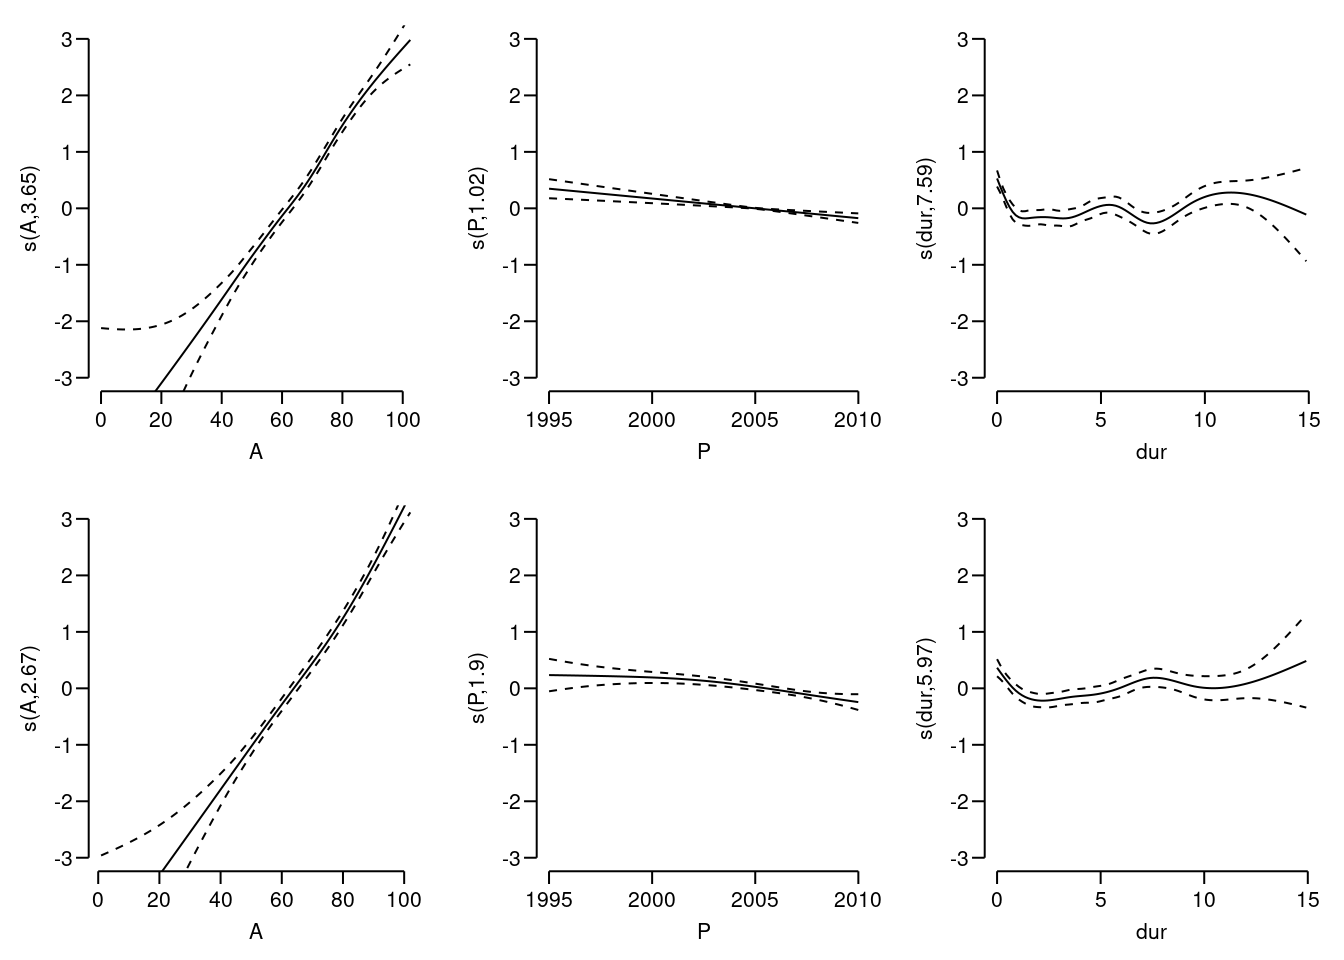
\includegraphics{DMDK-s_files/figure-latex/unnamed-chunk-15-1.pdf}

\begin{Shaded}
\begin{Highlighting}[]
\FunctionTok{par}\NormalTok{(}\AttributeTok{mfcol =} \FunctionTok{c}\NormalTok{(}\DecValTok{3}\NormalTok{, }\DecValTok{2}\NormalTok{))}
\FunctionTok{plot}\NormalTok{(Mcr, }\AttributeTok{ylim =} \FunctionTok{c}\NormalTok{(}\SpecialCharTok{{-}}\DecValTok{3}\NormalTok{, }\DecValTok{3}\NormalTok{))}
\FunctionTok{plot}\NormalTok{(Fcr, }\AttributeTok{ylim =} \FunctionTok{c}\NormalTok{(}\SpecialCharTok{{-}}\DecValTok{3}\NormalTok{, }\DecValTok{3}\NormalTok{))}
\end{Highlighting}
\end{Shaded}

  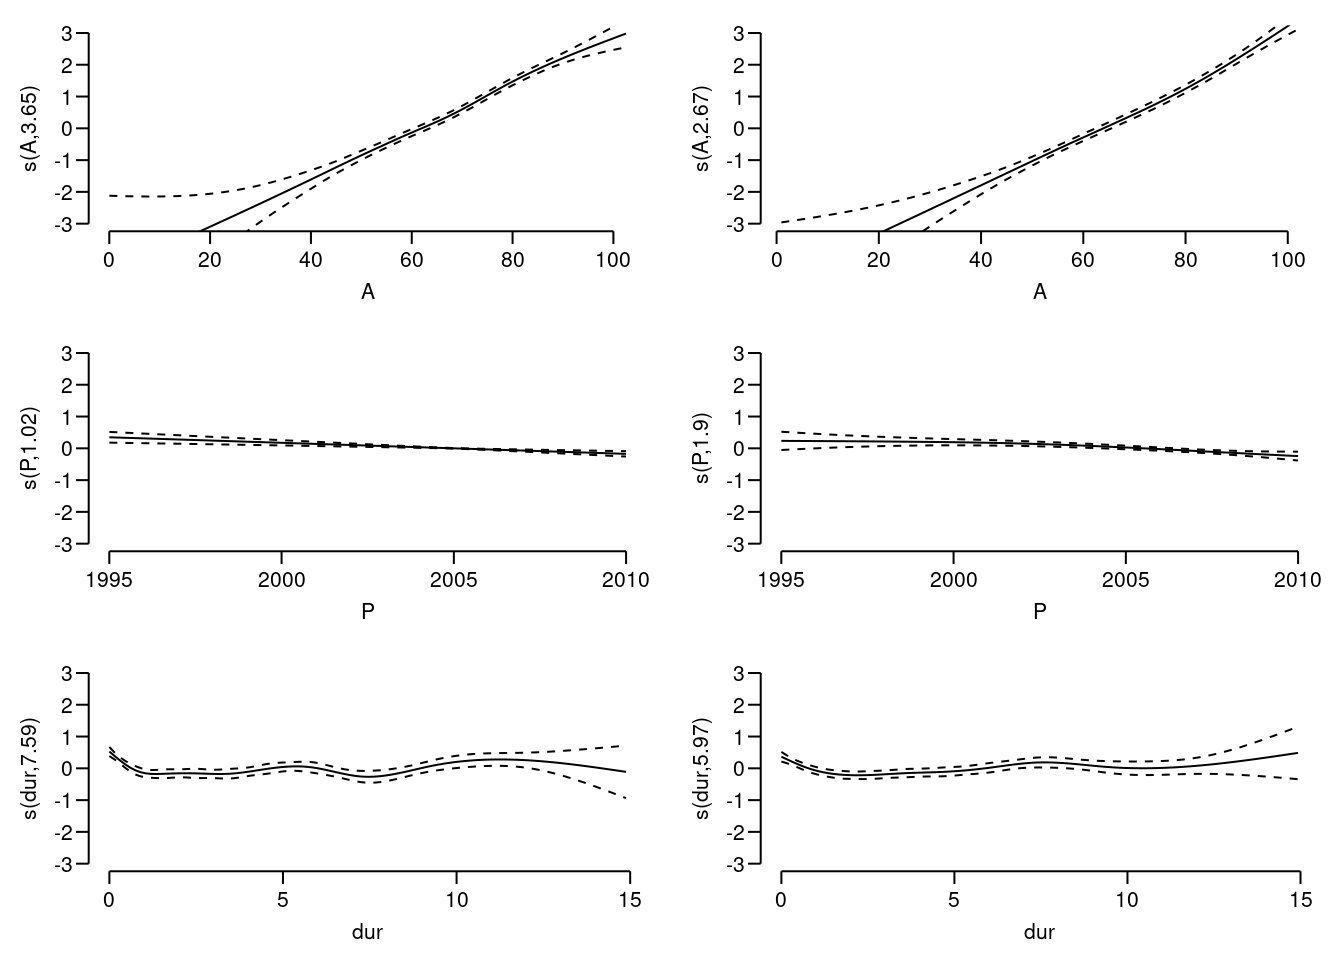
\includegraphics{DMDK-s_files/figure-latex/unnamed-chunk-16-1.pdf}
  What is the absolute scale for these effects?
\item
  Compare the fit of the naive model with just age and the
  three-factor models, using \texttt{anova}, e.g.:

\begin{Shaded}
\begin{Highlighting}[]
\FunctionTok{anova}\NormalTok{(Mcr, r.m, }\AttributeTok{test =} \StringTok{"Chisq"}\NormalTok{)}
\end{Highlighting}
\end{Shaded}

\begin{verbatim}
Analysis of Deviance Table

Model 1: cbind(trt(Lx$lex.Cst, Lx$lex.Xst) %in% trnam, Lx$lex.dur) ~ s(A, 
    bs = "cr", k = 10) + s(P, bs = "cr", k = 10) + s(dur, bs = "cr", 
    k = 10)
Model 2: cbind(trt(Lx$lex.Cst, Lx$lex.Xst) %in% trnam, Lx$lex.dur) ~ s(A, 
    k = 20)
  Resid. Df Resid. Dev      Df Deviance  Pr(>Chi)
1     60332      11717                           
2     60340      11812 -7.9484  -95.094 < 2.2e-16
\end{verbatim}

  What do you conclude?
\item
  The model we fitted has three time-scales: current age, current
  date and current duration of diabetes, so the effects that we report
  are not immediately interpretable, as they are (as in any kind of
  multiple regressions) to be interpreted as \emph{all else equal} which
  they are not, as the three time scales advance simultaneously at the
  same pace.

  The reporting would therefore more naturally be on the
  mortality scale as a function of age, but showing the mortality
  for persons diagnosed in different ages, using separate displays
  for separate years of diagnosis.
  This is most easily done using the \texttt{ci.pred} function with
  the \texttt{newdata\ =} argument. So a person diagnosed in age 50 in
  1995 will have a mortality measured in cases per 1000 PY as:

\begin{Shaded}
\begin{Highlighting}[]
\NormalTok{pts }\OtherTok{\textless{}{-}} \FunctionTok{seq}\NormalTok{(}\DecValTok{0}\NormalTok{, }\DecValTok{12}\NormalTok{, }\DecValTok{1}\SpecialCharTok{/}\DecValTok{4}\NormalTok{)}
\NormalTok{nd }\OtherTok{\textless{}{-}} \FunctionTok{data.frame}\NormalTok{(}\AttributeTok{A =} \DecValTok{50}   \SpecialCharTok{+}\NormalTok{ pts, }
                 \AttributeTok{P =} \DecValTok{1995} \SpecialCharTok{+}\NormalTok{ pts, }
               \AttributeTok{dur =}\NormalTok{        pts)}
\NormalTok{m.pr }\OtherTok{\textless{}{-}} \FunctionTok{ci.pred}\NormalTok{(Mcr, }\AttributeTok{newdata =}\NormalTok{ nd)}
\end{Highlighting}
\end{Shaded}

  Note that because we used \texttt{gam.Lexis} which uses
  the \texttt{poisreg} family we need not specify \texttt{lex.dur} as a
  variable in the prediction data frame \texttt{nd}. Predictions will
  be rates in the same units as \texttt{lex.dur} (well, the inverse).

  Now take a look at the result from the \texttt{ci.pred} statement and
  construct prediction of mortality for men and women diagnosed in a
  range of ages, say 50, 60, 70, and plot these together in the same
  graph:

\begin{Shaded}
\begin{Highlighting}[]
\FunctionTok{cbind}\NormalTok{(nd, }\FunctionTok{ci.pred}\NormalTok{(Mcr, }\AttributeTok{newdata =}\NormalTok{ nd))[}\DecValTok{1}\SpecialCharTok{:}\DecValTok{10}\NormalTok{,]}
\end{Highlighting}
\end{Shaded}
\item
  From figure it seems that the duration effect is
  over-modeled, so refit constraining the d.f. to 5:

\begin{Shaded}
\begin{Highlighting}[]
\NormalTok{Mcr }\OtherTok{\textless{}{-}} \FunctionTok{gam.Lexis}\NormalTok{(}\FunctionTok{subset}\NormalTok{(SL, sex }\SpecialCharTok{==} \StringTok{"M"}\NormalTok{),}
                 \SpecialCharTok{\textasciitilde{}} \FunctionTok{s}\NormalTok{(A, }\AttributeTok{bs =} \StringTok{"cr"}\NormalTok{, }\AttributeTok{k =} \DecValTok{10}\NormalTok{) }\SpecialCharTok{+}
                   \FunctionTok{s}\NormalTok{(P, }\AttributeTok{bs =} \StringTok{"cr"}\NormalTok{, }\AttributeTok{k =} \DecValTok{10}\NormalTok{) }\SpecialCharTok{+}
                 \FunctionTok{s}\NormalTok{(dur, }\AttributeTok{bs =} \StringTok{"cr"}\NormalTok{, }\AttributeTok{k =} \DecValTok{5}\NormalTok{))}
\end{Highlighting}
\end{Shaded}

\begin{verbatim}
mgcv::gam Poisson analysis of Lexis object subset(SL, sex == "M") with log link:
Rates for the transition:
Alive->Dead
\end{verbatim}

\begin{Shaded}
\begin{Highlighting}[]
\NormalTok{Fcr }\OtherTok{\textless{}{-}} \FunctionTok{gam.Lexis}\NormalTok{(}\FunctionTok{subset}\NormalTok{(SL, sex }\SpecialCharTok{==} \StringTok{"F"}\NormalTok{),}
                 \SpecialCharTok{\textasciitilde{}} \FunctionTok{s}\NormalTok{(A, }\AttributeTok{bs =} \StringTok{"cr"}\NormalTok{, }\AttributeTok{k =} \DecValTok{10}\NormalTok{) }\SpecialCharTok{+}
                   \FunctionTok{s}\NormalTok{(P, }\AttributeTok{bs =} \StringTok{"cr"}\NormalTok{, }\AttributeTok{k =} \DecValTok{10}\NormalTok{) }\SpecialCharTok{+}
                 \FunctionTok{s}\NormalTok{(dur, }\AttributeTok{bs =} \StringTok{"cr"}\NormalTok{, }\AttributeTok{k =} \DecValTok{5}\NormalTok{))}
\end{Highlighting}
\end{Shaded}

\begin{verbatim}
mgcv::gam Poisson analysis of Lexis object subset(SL, sex == "F") with log link:
Rates for the transition:
Alive->Dead
\end{verbatim}

  Plot the estimated rates from the revised models.
  What do you conclude from the plots?
\end{enumerate}

\section{SMR}\label{smr}

The SMR is the \textbf{S}tandardized \textbf{M}ortality
\textbf{R}atio, which is the mortality rate-ratio between the diabetes
patients and the general population. In real studies we would
subtract the deaths and the person-years among the diabetes patients
from those of the general population, but since we do not have access
to these, we make the comparison to the general population at large,
\emph{i.e.} also including the diabetes patients.

So we now want to include the population mortality rates as a fixed
variable in the split dataset; for each record in the split dataset we
attach the value of the population mortality for the relevant sex, and
and calendar time.

This can be achieved in two ways: Either we just use the current split
of follow-up time and allocate the population mortality rates for some
suitably chosen (mid-)point of the follow-up in each, or we make a
second split by date, so that follow-up in the diabetes patients is in
the same classification of age and data as the population mortality
table.

\begin{enumerate}
\def\labelenumi{\arabic{enumi}.}
\setcounter{enumi}{11}
\item
  We will use the former approach, using the dataset split in
  6 month intervals, and then include as an extra variable the
  population mortality as available from the data set \texttt{M.dk}.

  First create the variables in the diabetes dataset that we need
  for matching with the population mortality data, that is sex and
  age and date at the midpoint of each of the intervals (or rather at a
  point 3 months after the left endpoint of the interval; recall
  we split the follow-up in 6 month intervals).

  We need to have variables of the same type when we merge, so we must
  transform the sex variable in \texttt{M.dk} to a factor, and must
  for each follow-up interval in the \texttt{SL} data have an age and
  a period variable that can be used in merging with the population data.

\begin{Shaded}
\begin{Highlighting}[]
\FunctionTok{str}\NormalTok{(SL)}
\end{Highlighting}
\end{Shaded}

\begin{verbatim}
Classes 'Lexis' and 'data.frame':   118473 obs. of  14 variables:
 $ lex.id : int  1 1 1 1 1 1 1 1 1 1 ...
 $ A      : num  58.7 59 59.5 60 60.5 ...
 $ P      : num  1999 1999 2000 2000 2001 ...
 $ dur    : num  0 0.339 0.839 1.339 1.839 ...
 $ lex.dur: num  0.339 0.5 0.5 0.5 0.5 ...
 $ lex.Cst: Factor w/ 2 levels "Alive","Dead": 1 1 1 1 1 1 1 1 1 1 ...
 $ lex.Xst: Factor w/ 2 levels "Alive","Dead": 1 1 1 1 1 1 1 1 1 1 ...
 $ sex    : Factor w/ 2 levels "M","F": 2 2 2 2 2 2 2 2 2 2 ...
 $ dobth  : num  1940 1940 1940 1940 1940 ...
 $ dodm   : num  1999 1999 1999 1999 1999 ...
 $ dodth  : num  NA NA NA NA NA NA NA NA NA NA ...
 $ dooad  : num  NA NA NA NA NA NA NA NA NA NA ...
 $ doins  : num  NA NA NA NA NA NA NA NA NA NA ...
 $ dox    : num  2010 2010 2010 2010 2010 ...
 - attr(*, "breaks")=List of 3
  ..$ A  : num [1:251] 0 0.5 1 1.5 2 2.5 3 3.5 4 4.5 ...
  ..$ P  : NULL
  ..$ dur: NULL
 - attr(*, "time.scales")= chr [1:3] "A" "P" "dur"
 - attr(*, "time.since")= chr [1:3] "" "" ""
\end{verbatim}

\begin{Shaded}
\begin{Highlighting}[]
\NormalTok{SL}\SpecialCharTok{$}\NormalTok{Am }\OtherTok{\textless{}{-}} \FunctionTok{floor}\NormalTok{(SL}\SpecialCharTok{$}\NormalTok{A }\SpecialCharTok{+} \FloatTok{0.25}\NormalTok{)}
\NormalTok{SL}\SpecialCharTok{$}\NormalTok{Pm }\OtherTok{\textless{}{-}} \FunctionTok{floor}\NormalTok{(SL}\SpecialCharTok{$}\NormalTok{P }\SpecialCharTok{+} \FloatTok{0.25}\NormalTok{)}
\FunctionTok{data}\NormalTok{(M.dk)}
\FunctionTok{str}\NormalTok{(M.dk)}
\end{Highlighting}
\end{Shaded}

\begin{verbatim}
'data.frame':   7800 obs. of  6 variables:
 $ A   : num  0 0 0 0 0 0 0 0 0 0 ...
 $ sex : num  1 2 1 2 1 2 1 2 1 2 ...
 $ P   : num  1974 1974 1975 1975 1976 ...
 $ D   : num  459 303 435 311 405 258 332 205 312 233 ...
 $ Y   : num  35963 34383 36099 34652 34965 ...
 $ rate: num  12.76 8.81 12.05 8.97 11.58 ...
 - attr(*, "Contents")= chr "Number of deaths and risk time in Denmark"
\end{verbatim}

\begin{Shaded}
\begin{Highlighting}[]
\NormalTok{M.dk }\OtherTok{\textless{}{-}} \FunctionTok{transform}\NormalTok{(M.dk,}
                  \AttributeTok{Am =}\NormalTok{ A,}
                  \AttributeTok{Pm =}\NormalTok{ P,}
                 \AttributeTok{sex =} \FunctionTok{factor}\NormalTok{(sex, }\AttributeTok{labels =} \FunctionTok{c}\NormalTok{(}\StringTok{"M"}\NormalTok{, }\StringTok{"F"}\NormalTok{)))}
\FunctionTok{str}\NormalTok{(M.dk)}
\end{Highlighting}
\end{Shaded}

\begin{verbatim}
'data.frame':   7800 obs. of  8 variables:
 $ A   : num  0 0 0 0 0 0 0 0 0 0 ...
 $ sex : Factor w/ 2 levels "M","F": 1 2 1 2 1 2 1 2 1 2 ...
 $ P   : num  1974 1974 1975 1975 1976 ...
 $ D   : num  459 303 435 311 405 258 332 205 312 233 ...
 $ Y   : num  35963 34383 36099 34652 34965 ...
 $ rate: num  12.76 8.81 12.05 8.97 11.58 ...
 $ Am  : num  0 0 0 0 0 0 0 0 0 0 ...
 $ Pm  : num  1974 1974 1975 1975 1976 ...
\end{verbatim}

  Then match the rates from \texttt{M.dk} into \texttt{SL};
  \texttt{sex}, \texttt{Am} and \texttt{Pm} are the common variables,
  and therefore the match is on these variables:

\begin{Shaded}
\begin{Highlighting}[]
\NormalTok{SLr }\OtherTok{\textless{}{-}} \FunctionTok{merge}\NormalTok{(SL, }
\NormalTok{             M.dk[, }\FunctionTok{c}\NormalTok{(}\StringTok{"sex"}\NormalTok{, }\StringTok{"Am"}\NormalTok{, }\StringTok{"Pm"}\NormalTok{, }\StringTok{"rate"}\NormalTok{)])}
\FunctionTok{dim}\NormalTok{(SL)}
\end{Highlighting}
\end{Shaded}

\begin{verbatim}
[1] 118473     16
\end{verbatim}

\begin{Shaded}
\begin{Highlighting}[]
\FunctionTok{dim}\NormalTok{(SLr)}
\end{Highlighting}
\end{Shaded}

\begin{verbatim}
[1] 118454     17
\end{verbatim}

  This merge (remember to \texttt{?merge}!) only takes rows that have
  information from both datasets, hence the slightly fewer rows in
  \texttt{SLr} than in \texttt{SL}.

  \begin{itemize}
  \tightlist
  \item
    Compute the expected number of deaths as the person-time
    multiplied (\texttt{lex.dur}) by the corresponding population rate, and put it in a
    new variable, \texttt{E}, say (\texttt{E}xpected). Use \texttt{stat.table}
    to make a table of observed, expected and the ratio (SMR) by age
    (suitably grouped, look for \texttt{cut}) and sex.
  \end{itemize}
\item
  Fit a poisson model with sex as the explanatory variable and
  log-expected as offset to derive the SMR (and c.i.).
  Some of the population mortality rates are 0, so you need to exclude
  those records from the analysis.

\begin{Shaded}
\begin{Highlighting}[]
\NormalTok{msmr }\OtherTok{\textless{}{-}} \FunctionTok{glm}\NormalTok{((lex.Xst }\SpecialCharTok{==} \StringTok{"Dead"}\NormalTok{) }\SpecialCharTok{\textasciitilde{}}\NormalTok{ sex }\SpecialCharTok{{-}} \DecValTok{1}\NormalTok{,}
            \AttributeTok{offset =} \FunctionTok{log}\NormalTok{(E),}
            \AttributeTok{family =}\NormalTok{ poisson,}
              \AttributeTok{data =} \FunctionTok{subset}\NormalTok{(SLr, E }\SpecialCharTok{\textgreater{}} \DecValTok{0}\NormalTok{))}
\FunctionTok{ci.exp}\NormalTok{(msmr)}
\end{Highlighting}
\end{Shaded}

\begin{verbatim}
     exp(Est.)     2.5%    97.5%
sexM  1.685699 1.597881 1.778344
sexF  1.541922 1.455442 1.633540
\end{verbatim}

  Do you recognize the numbers?

  \begin{itemize}
  \tightlist
  \item
    The same model can be fitted a bit simpler by the \texttt{poisreg} family, try:
  \end{itemize}

\begin{Shaded}
\begin{Highlighting}[]
\NormalTok{msmr }\OtherTok{\textless{}{-}} \FunctionTok{glm}\NormalTok{(}\FunctionTok{cbind}\NormalTok{(lex.Xst }\SpecialCharTok{==} \StringTok{"Dead"}\NormalTok{, E) }\SpecialCharTok{\textasciitilde{}}\NormalTok{ sex }\SpecialCharTok{{-}} \DecValTok{1}\NormalTok{, }
            \AttributeTok{family =}\NormalTok{ poisreg,}
              \AttributeTok{data =} \FunctionTok{subset}\NormalTok{(SLr, E }\SpecialCharTok{\textgreater{}} \DecValTok{0}\NormalTok{))}
\FunctionTok{ci.exp}\NormalTok{(msmr)}
\end{Highlighting}
\end{Shaded}

\begin{verbatim}
     exp(Est.)     2.5%    97.5%
sexM  1.685699 1.597881 1.778344
sexF  1.541922 1.455441 1.633541
\end{verbatim}

  We can assess the ratios of SMRs between men and women by using the
  \texttt{ctr.mat} argument which should be a matrix:

\begin{Shaded}
\begin{Highlighting}[]
\NormalTok{(CM }\OtherTok{\textless{}{-}} \FunctionTok{rbind}\NormalTok{(}\AttributeTok{M =} \FunctionTok{c}\NormalTok{(}\DecValTok{1}\NormalTok{, }\DecValTok{0}\NormalTok{),}
             \AttributeTok{W =} \FunctionTok{c}\NormalTok{(}\DecValTok{0}\NormalTok{, }\DecValTok{1}\NormalTok{),}
         \StringTok{"M/F"} \OtherTok{=} \FunctionTok{c}\NormalTok{(}\DecValTok{1}\NormalTok{, }\SpecialCharTok{{-}}\DecValTok{1}\NormalTok{)))}
\end{Highlighting}
\end{Shaded}

\begin{verbatim}
    [,1] [,2]
M      1    0
W      0    1
M/F    1   -1
\end{verbatim}

\begin{Shaded}
\begin{Highlighting}[]
\FunctionTok{round}\NormalTok{(}\FunctionTok{ci.exp}\NormalTok{(msmr, }\AttributeTok{ctr.mat =}\NormalTok{ CM), }\DecValTok{2}\NormalTok{)}
\end{Highlighting}
\end{Shaded}

\begin{verbatim}
    exp(Est.) 2.5% 97.5%
M        1.69 1.60  1.78
W        1.54 1.46  1.63
M/F      1.09 1.01  1.18
\end{verbatim}

  What do you conclude about the mortality rates among men and women?
\end{enumerate}

\section{SMR modeling}\label{smr-modeling}

\begin{enumerate}
\def\labelenumi{\arabic{enumi}.}
\setcounter{enumi}{13}
\item
  Now model the SMR using age and date of diagnosis and diabetes
  duration as explanatory variables, including the expected-number
  instead of the person-years, using separate models for
  men and women.

  Note that you cannot use \texttt{gam.Lexis} from the code you used for
  fitting models for the rates, you need to use \texttt{gam} with
  the \texttt{poisreg} family. And remember to exclude those units
  where no deaths in the population occur (that is where the
  population mortality rate is 0).

\begin{Shaded}
\begin{Highlighting}[]
\NormalTok{Msmr }\OtherTok{\textless{}{-}} \FunctionTok{gam}\NormalTok{(}\FunctionTok{cbind}\NormalTok{(lex.Xst }\SpecialCharTok{==} \StringTok{"Dead"}\NormalTok{, E) }
            \SpecialCharTok{\textasciitilde{}} \FunctionTok{s}\NormalTok{(  A, }\AttributeTok{bs =} \StringTok{"cr"}\NormalTok{, }\AttributeTok{k =} \DecValTok{5}\NormalTok{) }\SpecialCharTok{+}
              \FunctionTok{s}\NormalTok{(  P, }\AttributeTok{bs =} \StringTok{"cr"}\NormalTok{, }\AttributeTok{k =} \DecValTok{5}\NormalTok{) }\SpecialCharTok{+}
              \FunctionTok{s}\NormalTok{(dur, }\AttributeTok{bs =} \StringTok{"cr"}\NormalTok{, }\AttributeTok{k =} \DecValTok{5}\NormalTok{),}
            \AttributeTok{family =}\NormalTok{ poisreg,}
              \AttributeTok{data =} \FunctionTok{subset}\NormalTok{(SLr, E }\SpecialCharTok{\textgreater{}} \DecValTok{0} \SpecialCharTok{\&}\NormalTok{ sex }\SpecialCharTok{==} \StringTok{"M"}\NormalTok{))}
\FunctionTok{ci.exp}\NormalTok{(Msmr)}
\end{Highlighting}
\end{Shaded}

\begin{verbatim}
            exp(Est.)      2.5%     97.5%
(Intercept) 2.1667053 2.0001046 2.3471833
s(A).1      0.5960527 0.5181962 0.6856068
s(A).2      0.8927331 0.8650901 0.9212594
s(A).3      0.3663506 0.2818154 0.4762435
s(A).4      0.4587803 0.3763049 0.5593320
s(P).1      0.9893048 0.9732835 1.0055898
s(P).2      0.9608720 0.9085181 1.0162428
s(P).3      0.9027294 0.7825209 1.0414040
s(P).4      0.9173557 0.8132938 1.0347323
s(dur).1    0.6581828 0.5769629 0.7508362
s(dur).2    0.8446645 0.7613599 0.9370838
s(dur).3    0.7830215 0.6916313 0.8864877
s(dur).4    1.8176744 1.1041338 2.9923368
\end{verbatim}

\begin{Shaded}
\begin{Highlighting}[]
\NormalTok{Fsmr }\OtherTok{\textless{}{-}} \FunctionTok{update}\NormalTok{(Msmr, }\AttributeTok{data =} \FunctionTok{subset}\NormalTok{(SLr, E }\SpecialCharTok{\textgreater{}} \DecValTok{0} \SpecialCharTok{\&}\NormalTok{ sex }\SpecialCharTok{==} \StringTok{"F"}\NormalTok{))}
\end{Highlighting}
\end{Shaded}

  Plot the estimated smooth effects for both men and women using
  e.g.~\texttt{plot.gam}. What do you see?
\item
  Plot the predicted SMRs from the models for men and women
  diagnosed in ages 50, 60 and 70 as you did for the rates. What do
  you see?

\begin{Shaded}
\begin{Highlighting}[]
\FunctionTok{par}\NormalTok{(}\AttributeTok{mfrow =} \FunctionTok{c}\NormalTok{(}\DecValTok{1}\NormalTok{,}\DecValTok{1}\NormalTok{))}
\NormalTok{n50 }\OtherTok{\textless{}{-}}\NormalTok{ nd}
\NormalTok{n60 }\OtherTok{\textless{}{-}} \FunctionTok{mutate}\NormalTok{(n50, }\AttributeTok{A =}\NormalTok{ A }\SpecialCharTok{+} \DecValTok{10}\NormalTok{)}
\NormalTok{n70 }\OtherTok{\textless{}{-}} \FunctionTok{mutate}\NormalTok{(n50, }\AttributeTok{A =}\NormalTok{ A }\SpecialCharTok{+} \DecValTok{20}\NormalTok{)}
\FunctionTok{head}\NormalTok{(n70)}
\end{Highlighting}
\end{Shaded}

\begin{verbatim}
      A       P  dur
1 70.00 1995.00 0.00
2 70.25 1995.25 0.25
3 70.50 1995.50 0.50
4 70.75 1995.75 0.75
5 71.00 1996.00 1.00
6 71.25 1996.25 1.25
\end{verbatim}

\begin{Shaded}
\begin{Highlighting}[]
\FunctionTok{matshade}\NormalTok{(n50}\SpecialCharTok{$}\NormalTok{A, }\FunctionTok{cbind}\NormalTok{(}\FunctionTok{ci.pred}\NormalTok{(Msmr, n50),}
                      \FunctionTok{ci.pred}\NormalTok{(Fsmr, n50)), }\AttributeTok{plot =} \ConstantTok{TRUE}\NormalTok{,}
         \AttributeTok{col =} \FunctionTok{c}\NormalTok{(}\StringTok{"blue"}\NormalTok{, }\StringTok{"red"}\NormalTok{), }\AttributeTok{lwd =} \DecValTok{3}\NormalTok{,}
         \AttributeTok{ylim =} \FunctionTok{c}\NormalTok{(}\FloatTok{0.5}\NormalTok{, }\DecValTok{5}\NormalTok{), }\AttributeTok{log  =} \StringTok{"y"}\NormalTok{, }\AttributeTok{xlim =} \FunctionTok{c}\NormalTok{(}\DecValTok{50}\NormalTok{, }\DecValTok{80}\NormalTok{))}
\FunctionTok{matshade}\NormalTok{(n60}\SpecialCharTok{$}\NormalTok{A, }\FunctionTok{cbind}\NormalTok{(}\FunctionTok{ci.pred}\NormalTok{(Msmr, n60),}
                      \FunctionTok{ci.pred}\NormalTok{(Fsmr, n60)),}
         \AttributeTok{col =} \FunctionTok{c}\NormalTok{(}\StringTok{"blue"}\NormalTok{, }\StringTok{"red"}\NormalTok{), }\AttributeTok{lwd =} \DecValTok{3}\NormalTok{)}
\FunctionTok{matshade}\NormalTok{(n70}\SpecialCharTok{$}\NormalTok{A, }\FunctionTok{cbind}\NormalTok{(}\FunctionTok{ci.pred}\NormalTok{(Msmr, n70),}
                      \FunctionTok{ci.pred}\NormalTok{(Fsmr, n70)),}
         \AttributeTok{col =} \FunctionTok{c}\NormalTok{(}\StringTok{"blue"}\NormalTok{, }\StringTok{"red"}\NormalTok{), }\AttributeTok{lwd =} \DecValTok{3}\NormalTok{)}
\FunctionTok{abline}\NormalTok{(}\AttributeTok{h =} \DecValTok{1}\NormalTok{)}
\FunctionTok{abline}\NormalTok{(}\AttributeTok{v =} \DecValTok{50} \SpecialCharTok{+} \DecValTok{0}\SpecialCharTok{:}\DecValTok{5}\NormalTok{, }\AttributeTok{lty =} \DecValTok{3}\NormalTok{, }\AttributeTok{col =} \StringTok{"gray"}\NormalTok{)}
\end{Highlighting}
\end{Shaded}

  \includegraphics{DMDK-s_files/figure-latex/unnamed-chunk-27-1.pdf}
  Describe the shapes of the curves. What aspects of the shapes are
  induced by the model ?
\item
  Try to simplify the model to one with a simple sex effect,
  separate linear effects of age and date of follow-up for each
  sex, and a smooth effect of duration common for both sexes,
  giving an estimate of the change in SMR by age and calendar
  time.

\begin{Shaded}
\begin{Highlighting}[]
\NormalTok{Bsmr }\OtherTok{\textless{}{-}} \FunctionTok{gam}\NormalTok{(}\FunctionTok{cbind}\NormalTok{(lex.Xst }\SpecialCharTok{==} \StringTok{"Dead"}\NormalTok{, E) }
            \SpecialCharTok{\textasciitilde{}}\NormalTok{ sex }\SpecialCharTok{/}\NormalTok{ A }\SpecialCharTok{+}
\NormalTok{              sex }\SpecialCharTok{/}\NormalTok{ P }\SpecialCharTok{+}
              \FunctionTok{s}\NormalTok{(dur, }\AttributeTok{bs =} \StringTok{"cr"}\NormalTok{, }\AttributeTok{k =} \DecValTok{5}\NormalTok{),}
            \AttributeTok{family =}\NormalTok{ poisreg,}
              \AttributeTok{data =} \FunctionTok{subset}\NormalTok{(SLr, E }\SpecialCharTok{\textgreater{}} \DecValTok{0}\NormalTok{))}
\FunctionTok{round}\NormalTok{(}\FunctionTok{ci.exp}\NormalTok{(Bsmr)[}\SpecialCharTok{{-}}\DecValTok{1}\NormalTok{,], }\DecValTok{3}\NormalTok{)}
\end{Highlighting}
\end{Shaded}

\begin{verbatim}
         exp(Est.)  2.5%        97.5%
sexF     52149.525 0.000 2.375788e+23
sexM:A       0.981 0.977 9.860000e-01
sexF:A       0.980 0.975 9.860000e-01
sexM:P       0.987 0.972 1.002000e+00
sexF:P       0.981 0.965 9.980000e-01
s(dur).1     0.663 0.601 7.320000e-01
s(dur).2     0.861 0.795 9.310000e-01
s(dur).3     0.885 0.805 9.740000e-01
s(dur).4     1.412 0.945 2.111000e+00
\end{verbatim}

  How much does SMR change by each year of age? And by each
  calendar year?

  What is the meaning of the \texttt{sexF} parameter?
\item
  Use your previous code to plot the predicted mortality from this
  model too. Are the predicted SMR curves credible?

\begin{Shaded}
\begin{Highlighting}[]
\NormalTok{m50 }\OtherTok{\textless{}{-}} \FunctionTok{mutate}\NormalTok{(n50, }\AttributeTok{sex =} \StringTok{"M"}\NormalTok{)}
\NormalTok{f50 }\OtherTok{\textless{}{-}} \FunctionTok{mutate}\NormalTok{(n50, }\AttributeTok{sex =} \StringTok{"F"}\NormalTok{)}
\NormalTok{m60 }\OtherTok{\textless{}{-}} \FunctionTok{mutate}\NormalTok{(m50, }\AttributeTok{A =}\NormalTok{ A }\SpecialCharTok{+} \DecValTok{10}\NormalTok{)}
\NormalTok{f60 }\OtherTok{\textless{}{-}} \FunctionTok{mutate}\NormalTok{(f50, }\AttributeTok{A =}\NormalTok{ A }\SpecialCharTok{+} \DecValTok{10}\NormalTok{)}
\NormalTok{m70 }\OtherTok{\textless{}{-}} \FunctionTok{mutate}\NormalTok{(m50, }\AttributeTok{A =}\NormalTok{ A }\SpecialCharTok{+} \DecValTok{20}\NormalTok{)}
\NormalTok{f70 }\OtherTok{\textless{}{-}} \FunctionTok{mutate}\NormalTok{(f50, }\AttributeTok{A =}\NormalTok{ A }\SpecialCharTok{+} \DecValTok{20}\NormalTok{)}
\FunctionTok{matshade}\NormalTok{(n50}\SpecialCharTok{$}\NormalTok{A, }\FunctionTok{cbind}\NormalTok{(}\FunctionTok{ci.pred}\NormalTok{(Bsmr, m50),}
                      \FunctionTok{ci.pred}\NormalTok{(Bsmr, f50)), }\AttributeTok{plot =} \ConstantTok{TRUE}\NormalTok{,}
         \AttributeTok{col =} \FunctionTok{c}\NormalTok{(}\StringTok{"blue"}\NormalTok{, }\StringTok{"red"}\NormalTok{), }\AttributeTok{lwd =} \DecValTok{3}\NormalTok{,}
         \AttributeTok{ylim =} \FunctionTok{c}\NormalTok{(}\FloatTok{0.5}\NormalTok{, }\DecValTok{5}\NormalTok{), }\AttributeTok{log  =} \StringTok{"y"}\NormalTok{, }\AttributeTok{xlim =} \FunctionTok{c}\NormalTok{(}\DecValTok{50}\NormalTok{, }\DecValTok{80}\NormalTok{))}
\FunctionTok{matshade}\NormalTok{(n60}\SpecialCharTok{$}\NormalTok{A, }\FunctionTok{cbind}\NormalTok{(}\FunctionTok{ci.pred}\NormalTok{(Bsmr, m60),}
                      \FunctionTok{ci.pred}\NormalTok{(Bsmr, f60)),}
         \AttributeTok{col =} \FunctionTok{c}\NormalTok{(}\StringTok{"blue"}\NormalTok{, }\StringTok{"red"}\NormalTok{), }\AttributeTok{lwd =} \DecValTok{3}\NormalTok{)}
\FunctionTok{matshade}\NormalTok{(n70}\SpecialCharTok{$}\NormalTok{A, }\FunctionTok{cbind}\NormalTok{(}\FunctionTok{ci.pred}\NormalTok{(Bsmr, m70),}
                      \FunctionTok{ci.pred}\NormalTok{(Bsmr, f70)),}
         \AttributeTok{col =} \FunctionTok{c}\NormalTok{(}\StringTok{"blue"}\NormalTok{, }\StringTok{"red"}\NormalTok{), }\AttributeTok{lwd =} \DecValTok{3}\NormalTok{)}
\FunctionTok{abline}\NormalTok{(}\AttributeTok{h =} \DecValTok{1}\NormalTok{)}
\FunctionTok{abline}\NormalTok{(}\AttributeTok{h =} \DecValTok{1}\SpecialCharTok{:}\DecValTok{5}\NormalTok{, }\AttributeTok{lty =} \DecValTok{3}\NormalTok{, }\AttributeTok{col =} \StringTok{"gray"}\NormalTok{)}
\end{Highlighting}
\end{Shaded}

  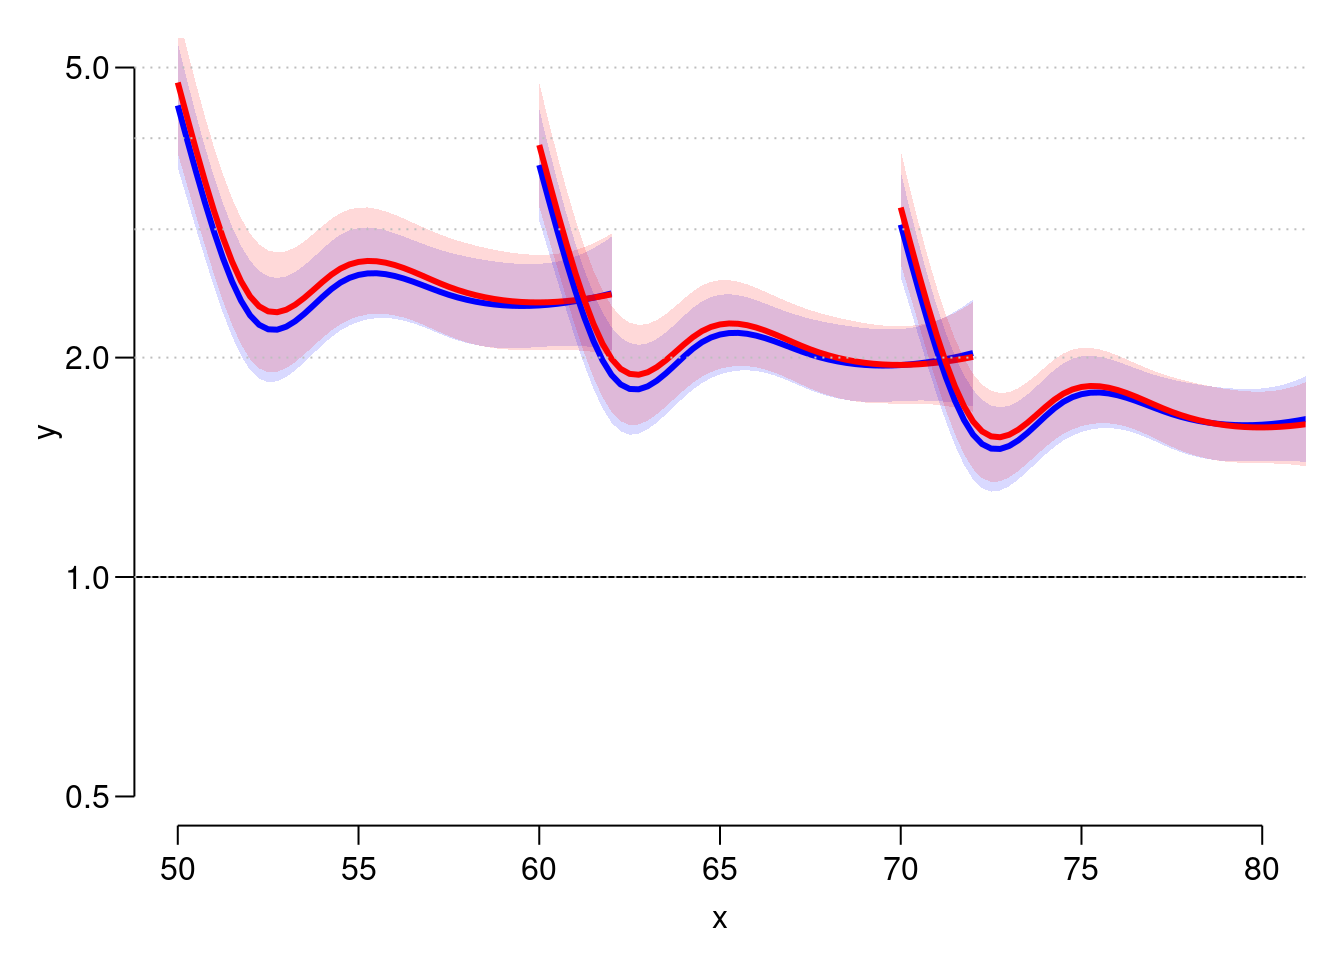
\includegraphics{DMDK-s_files/figure-latex/unnamed-chunk-29-1.pdf}
  What is your conclusion about SMR for diabetes patients relative to the
  general popuation?
\end{enumerate}

\chapter{Nested case-control study and case-cohort study: Risk factors of coronary heart disease}\label{nested-case-control-study-and-case-cohort-study-risk-factors-of-coronary-heart-disease}

In this exercise we shall apply both the nested case-control (NCC)
design and the case-cohort (CC) design in sampling
control subjects from a defined cohort or closed study population.
The case group comprises those cohort members who die from coronary heart disease (CHD) during a \(> 20\) years follow-up of the cohort.\\
The risk factors of interest are cigarette smoking, systolic blood pressure, and total cholesterol level.

Our study population is an occupational cohort comprising 1501 men
working in blue-collar jobs in one Nordic country.
Eligible subjects had no history of coronary heart disease
when recruited to the study in the early 1990s.
Smoking habits and many other items were inquired at baseline
by a questionnaire, and
blood pressure was measured by a research nurse, the values being
written down on the questionnaire. Serum samples were also taken from the cohort members at the same time and were stored in a freezer. For some reason,
the data in the questionnaires were not entered to any computer file, but the questionnaires were kept in a safe storehouse for further purposes.
Also, no biochemical analyses were initially performed for the sera
collected from the participants. However, dates of birth and dates of entry to the study were recorded
in an electronic file.

In 2010 the study was suddenly reactivated by those investigators of the original team who were still alive then.
As the first step mortality follow-up of the cohort members was
executed by record linkage to the national population register, from which
the dates of death and emigration were obtained. Another linkage was performed with the national register of causes of death in order to get the
deaths from coronary heard disease identified. As a result a data file
\texttt{occoh.txt} was completed containing the following variables:

\begin{longtable}[]{@{}
  >{\raggedright\arraybackslash}p{(\columnwidth - 2\tabcolsep) * \real{0.1569}}
  >{\raggedright\arraybackslash}p{(\columnwidth - 2\tabcolsep) * \real{0.8431}}@{}}
\toprule\noalign{}
\begin{minipage}[b]{\linewidth}\raggedright
Variable
\end{minipage} & \begin{minipage}[b]{\linewidth}\raggedright
Description
\end{minipage} \\
\midrule\noalign{}
\endhead
\bottomrule\noalign{}
\endlastfoot
\texttt{id} & identification number \\
\texttt{birth} & date of birth \\
\texttt{entry} & date of recruitment and baseline measurements \\
\texttt{exit} & date of exit from mortality follow-up \\
\texttt{death} & indicator for vital status at the end of follow-up; 1, if dead from any cause, and = 0, if alive \\
\texttt{chdeath} & indicator for death from coronary heart disease; 1, if \emph{yes}, and 0, if \emph{no}. \\
\end{longtable}

This exercise is divided into five main parts:

\begin{enumerate}
\def\labelenumi{\arabic{enumi}.}
\item
  Description of the study base or the follow-up experience of the
  whole cohort, identification of the cases and illustrating the risk sets.
\item
  Nested case-control study within the cohort:

  \begin{enumerate}
  \def\labelenumii{(\roman{enumii})}
  \tightlist
  \item
    selection of controls by risk set or time-matched sampling
    using function \texttt{ccwc()} in package \texttt{Epi},
  \item
    collection of exposure data for cases and controls
    from the pertinent data base of the whole cohort to the
    case-control data set using function \texttt{merge()}, and
  \item
    analysis of the case-control data set with stratified Cox
    model using function \texttt{clogit()} in package \texttt{survival()},
  \end{enumerate}
\item
  Case-cohort study within the cohort:

  \begin{enumerate}
  \def\labelenumii{(\roman{enumii})}
  \tightlist
  \item
    selection of a subcohort by simple random sampling from the cohort,
  \item
    collection of exposure data for subcohort members and cases, and
  \item
    analysis of the case-cohort data set with Cox model by weighted partial
    likelihood including appropriate weighting and correction of estimated
    covariance matrix for the model coefficients using function \texttt{cch()} in package \texttt{survival()}.
  \end{enumerate}
\item
  Comparison of results from all previous analyses, also with those from a full cohort design.
\item
  Further tasks and homework.
\end{enumerate}

\section{Reading the cohort data, illustrating the study base and risk sets}\label{reading-the-cohort-data-illustrating-the-study-base-and-risk-sets}

\begin{itemize}
\tightlist
\item
  Load the packages \texttt{Epi} and \texttt{survival}.
  Read in the cohort data file and name
  the resulting data frame as \texttt{oc}.
  See its structure and print the univariate summaries.
\end{itemize}

\begin{Shaded}
\begin{Highlighting}[]
\FunctionTok{library}\NormalTok{(Epi)}
\FunctionTok{library}\NormalTok{(survival)}
\NormalTok{url }\OtherTok{\textless{}{-}} \StringTok{"https://raw.githubusercontent.com/SPE{-}R/SPE/master/pracs/data"}
\NormalTok{oc }\OtherTok{\textless{}{-}} \FunctionTok{read.table}\NormalTok{(}\FunctionTok{paste}\NormalTok{(url, }\StringTok{"occoh.txt"}\NormalTok{, }\AttributeTok{sep =} \StringTok{"/"}\NormalTok{), }\AttributeTok{header =} \ConstantTok{TRUE}\NormalTok{)}
\FunctionTok{str}\NormalTok{(oc)}
\end{Highlighting}
\end{Shaded}

\begin{verbatim}
## 'data.frame':    1501 obs. of  6 variables:
##  $ id     : int  1 2 3 4 5 6 7 8 9 10 ...
##  $ birth  : chr  "1943-02-19" "1934-07-06" "1939-03-05" "1939-07-03" ...
##  $ entry  : chr  "1990-08-14" "1990-08-14" "1990-08-14" "1990-08-14" ...
##  $ exit   : chr  "2009-12-31" "2009-12-31" "2009-12-31" "2009-12-31" ...
##  $ death  : int  0 0 0 0 1 1 1 1 0 0 ...
##  $ chdeath: int  0 0 0 0 0 0 0 1 0 0 ...
\end{verbatim}

\begin{Shaded}
\begin{Highlighting}[]
\FunctionTok{summary}\NormalTok{(oc)}
\end{Highlighting}
\end{Shaded}

\begin{verbatim}
##        id          birth              entry               exit          
##  Min.   :   1   Length:1501        Length:1501        Length:1501       
##  1st Qu.: 376   Class :character   Class :character   Class :character  
##  Median : 751   Mode  :character   Mode  :character   Mode  :character  
##  Mean   : 751                                                           
##  3rd Qu.:1126                                                           
##  Max.   :1501                                                           
##      death           chdeath       
##  Min.   :0.0000   Min.   :0.00000  
##  1st Qu.:0.0000   1st Qu.:0.00000  
##  Median :0.0000   Median :0.00000  
##  Mean   :0.1972   Mean   :0.07995  
##  3rd Qu.:0.0000   3rd Qu.:0.00000  
##  Max.   :1.0000   Max.   :1.00000
\end{verbatim}

\begin{itemize}
\tightlist
\item
  It is convenient to change all the dates into fractional calendar years
\end{itemize}

\begin{Shaded}
\begin{Highlighting}[]
\NormalTok{oc}\SpecialCharTok{$}\NormalTok{ybirth }\OtherTok{\textless{}{-}} \FunctionTok{cal.yr}\NormalTok{(oc}\SpecialCharTok{$}\NormalTok{birth)}
\NormalTok{oc}\SpecialCharTok{$}\NormalTok{yentry }\OtherTok{\textless{}{-}} \FunctionTok{cal.yr}\NormalTok{(oc}\SpecialCharTok{$}\NormalTok{entry)}
\NormalTok{oc}\SpecialCharTok{$}\NormalTok{yexit }\OtherTok{\textless{}{-}} \FunctionTok{cal.yr}\NormalTok{(oc}\SpecialCharTok{$}\NormalTok{exit)}
\end{Highlighting}
\end{Shaded}

We shall also compute the age at entry and at exit, respectively,
as age will be the main time scale in our analyses.

\begin{Shaded}
\begin{Highlighting}[]
\NormalTok{oc}\SpecialCharTok{$}\NormalTok{agentry }\OtherTok{\textless{}{-}}\NormalTok{ oc}\SpecialCharTok{$}\NormalTok{yentry }\SpecialCharTok{{-}}\NormalTok{ oc}\SpecialCharTok{$}\NormalTok{ybirth}
\NormalTok{oc}\SpecialCharTok{$}\NormalTok{agexit }\OtherTok{\textless{}{-}}\NormalTok{ oc}\SpecialCharTok{$}\NormalTok{yexit }\SpecialCharTok{{-}}\NormalTok{ oc}\SpecialCharTok{$}\NormalTok{ybirth}
\end{Highlighting}
\end{Shaded}

\begin{itemize}
\tightlist
\item
  As the next step we shall create a \texttt{lexis} object
  from the data frame along the calendar period and age axes,
  and as the outcome event we specify the coronary death.
\end{itemize}

\begin{Shaded}
\begin{Highlighting}[]
\NormalTok{oc.lex }\OtherTok{\textless{}{-}} \FunctionTok{Lexis}\NormalTok{(}
  \AttributeTok{entry =} \FunctionTok{list}\NormalTok{(}
    \AttributeTok{per =}\NormalTok{ yentry,}
    \AttributeTok{age =}\NormalTok{ yentry }\SpecialCharTok{{-}}\NormalTok{ ybirth}
\NormalTok{  ),}
  \AttributeTok{exit =} \FunctionTok{list}\NormalTok{(}\AttributeTok{per =}\NormalTok{ yexit),}
  \AttributeTok{exit.status =}\NormalTok{ chdeath,}
  \AttributeTok{id =}\NormalTok{ id, }\AttributeTok{data =}\NormalTok{ oc}
\NormalTok{)}
\end{Highlighting}
\end{Shaded}

\begin{verbatim}
## NOTE: entry.status has been set to 0 for all.
\end{verbatim}

\begin{Shaded}
\begin{Highlighting}[]
\FunctionTok{str}\NormalTok{(oc.lex)}
\end{Highlighting}
\end{Shaded}

\begin{verbatim}
## Classes 'Lexis' and 'data.frame':    1501 obs. of  17 variables:
##  $ per    : 'cal.yr' num  1991 1991 1991 1991 1991 ...
##  $ age    : 'cal.yr' num  47.5 56.1 51.4 51.1 55.5 ...
##  $ lex.dur: 'cal.yr' num  19.4 19.4 19.4 19.4 15.6 ...
##  $ lex.Cst: num  0 0 0 0 0 0 0 0 0 0 ...
##  $ lex.Xst: int  0 0 0 0 0 0 0 1 0 0 ...
##  $ lex.id : int  1 2 3 4 5 6 7 8 9 10 ...
##  $ id     : int  1 2 3 4 5 6 7 8 9 10 ...
##  $ birth  : chr  "1943-02-19" "1934-07-06" "1939-03-05" "1939-07-03" ...
##  $ entry  : chr  "1990-08-14" "1990-08-14" "1990-08-14" "1990-08-14" ...
##  $ exit   : chr  "2009-12-31" "2009-12-31" "2009-12-31" "2009-12-31" ...
##  $ death  : int  0 0 0 0 1 1 1 1 0 0 ...
##  $ chdeath: int  0 0 0 0 0 0 0 1 0 0 ...
##  $ ybirth : 'cal.yr' num  1943 1935 1939 1940 1935 ...
##  $ yentry : 'cal.yr' num  1991 1991 1991 1991 1991 ...
##  $ yexit  : 'cal.yr' num  2010 2010 2010 2010 2006 ...
##  $ agentry: 'cal.yr' num  47.5 56.1 51.4 51.1 55.5 ...
##  $ agexit : 'cal.yr' num  66.9 75.5 70.8 70.5 71.1 ...
##  - attr(*, "time.scales")= chr [1:2] "per" "age"
##  - attr(*, "time.since")= chr [1:2] "" ""
##  - attr(*, "breaks")=List of 2
##   ..$ per: NULL
##   ..$ age: NULL
\end{verbatim}

\begin{Shaded}
\begin{Highlighting}[]
\FunctionTok{summary}\NormalTok{(oc.lex)}
\end{Highlighting}
\end{Shaded}

\begin{verbatim}
##     
## Transitions:
##      To
## From    0   1  Records:  Events: Risk time:  Persons:
##    0 1381 120      1501      120   25280.91      1501
\end{verbatim}

\begin{itemize}
\tightlist
\item
  At this stage it is informative to examine a graphical
  presentation of the follow-up lines and outcome cases in a conventional
  Lexis diagram. Make use of the \texttt{plot} method for \texttt{Lexis} objects.
  Gray lifelines are drawn and a bullet is put at the exit point of those lifelines
  that end with the outcome event.
\end{itemize}

\begin{Shaded}
\begin{Highlighting}[]
\FunctionTok{par}\NormalTok{(}\AttributeTok{mfrow =} \FunctionTok{c}\NormalTok{(}\DecValTok{1}\NormalTok{, }\DecValTok{1}\NormalTok{))}
\FunctionTok{plot}\NormalTok{(oc.lex, }\AttributeTok{xlim =} \FunctionTok{c}\NormalTok{(}\DecValTok{1990}\NormalTok{, }\DecValTok{2010}\NormalTok{), }\AttributeTok{grid =} \ConstantTok{TRUE}\NormalTok{)}
\FunctionTok{points}\NormalTok{(oc.lex, }\AttributeTok{pch =} \FunctionTok{c}\NormalTok{(}\ConstantTok{NA}\NormalTok{, }\DecValTok{16}\NormalTok{)[oc.lex}\SpecialCharTok{$}\NormalTok{lex.Xst }\SpecialCharTok{+} \DecValTok{1}\NormalTok{])}
\end{Highlighting}
\end{Shaded}

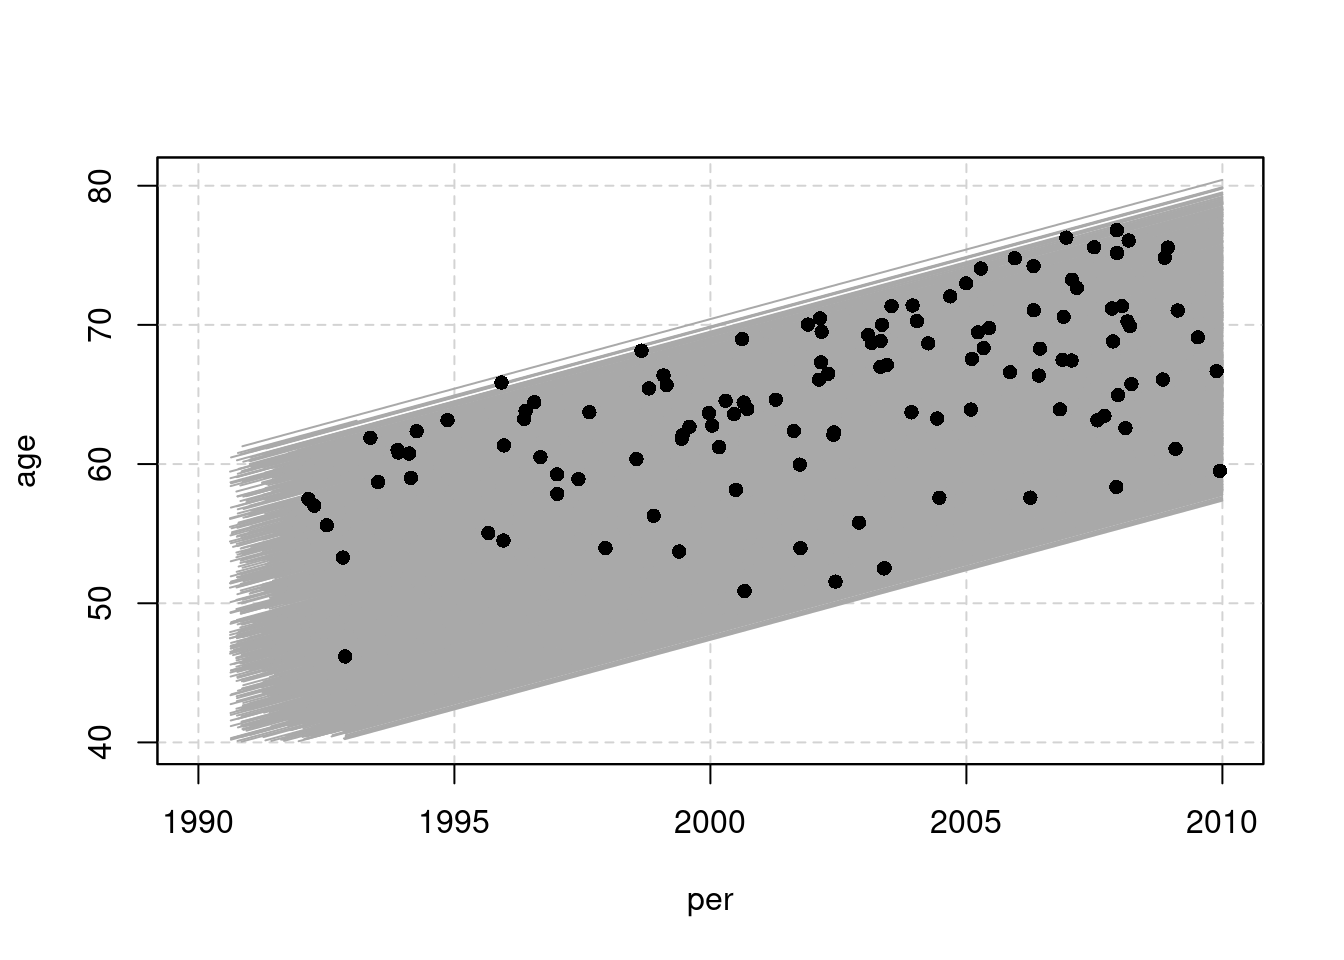
\includegraphics{occoh-caco-s_files/figure-latex/plotlexis-1.pdf}
- As age is here the main time axis,
we shall graphically illustrate the \textbf{study base}, \emph{i.e.}
the follow-up lines and outcome events,
only along the age scale, being ordered by age at exit.
Vertical lines at those ages when new coronary
deaths occur are drawn to identify the pertinent
\textbf{risk sets}. For that purpose it is useful first
to sort the data frame and the \texttt{Lexis} object
jointly by age at exit \& age at entry,
and to give a new ID number according to that order.

\begin{Shaded}
\begin{Highlighting}[]
\NormalTok{oc.ord }\OtherTok{\textless{}{-}} \FunctionTok{cbind}\NormalTok{(}\AttributeTok{ID =} \DecValTok{1}\SpecialCharTok{:}\DecValTok{1501}\NormalTok{, oc[}\FunctionTok{order}\NormalTok{(oc}\SpecialCharTok{$}\NormalTok{agexit, oc}\SpecialCharTok{$}\NormalTok{agentry), ])}
\NormalTok{oc.lexord }\OtherTok{\textless{}{-}} \FunctionTok{Lexis}\NormalTok{(}
  \AttributeTok{entry =} \FunctionTok{list}\NormalTok{(}\AttributeTok{age =}\NormalTok{ agentry),}
  \AttributeTok{exit =} \FunctionTok{list}\NormalTok{(}\AttributeTok{age =}\NormalTok{ agexit),}
  \AttributeTok{exit.status =}\NormalTok{ chdeath,}
  \AttributeTok{id =}\NormalTok{ ID, }\AttributeTok{data =}\NormalTok{ oc.ord}
\NormalTok{)}
\end{Highlighting}
\end{Shaded}

\begin{verbatim}
## NOTE: entry.status has been set to 0 for all.
\end{verbatim}

\begin{Shaded}
\begin{Highlighting}[]
\FunctionTok{plot}\NormalTok{(oc.lexord, }\StringTok{"age"}\NormalTok{)}
\FunctionTok{points}\NormalTok{(oc.lexord, }\AttributeTok{pch =} \FunctionTok{ifelse}\NormalTok{(oc.lexord}\SpecialCharTok{$}\NormalTok{lex.Xst }\SpecialCharTok{==} \DecValTok{1}\NormalTok{, }\DecValTok{16}\NormalTok{, }\ConstantTok{NA}\NormalTok{))}
\FunctionTok{with}\NormalTok{(}
  \FunctionTok{subset}\NormalTok{(oc.lexord, lex.Xst }\SpecialCharTok{==} \DecValTok{1}\NormalTok{),}
  \FunctionTok{abline}\NormalTok{(}\AttributeTok{v =}\NormalTok{ agexit, }\AttributeTok{lty =} \DecValTok{3}\NormalTok{)}
\NormalTok{)}
\end{Highlighting}
\end{Shaded}

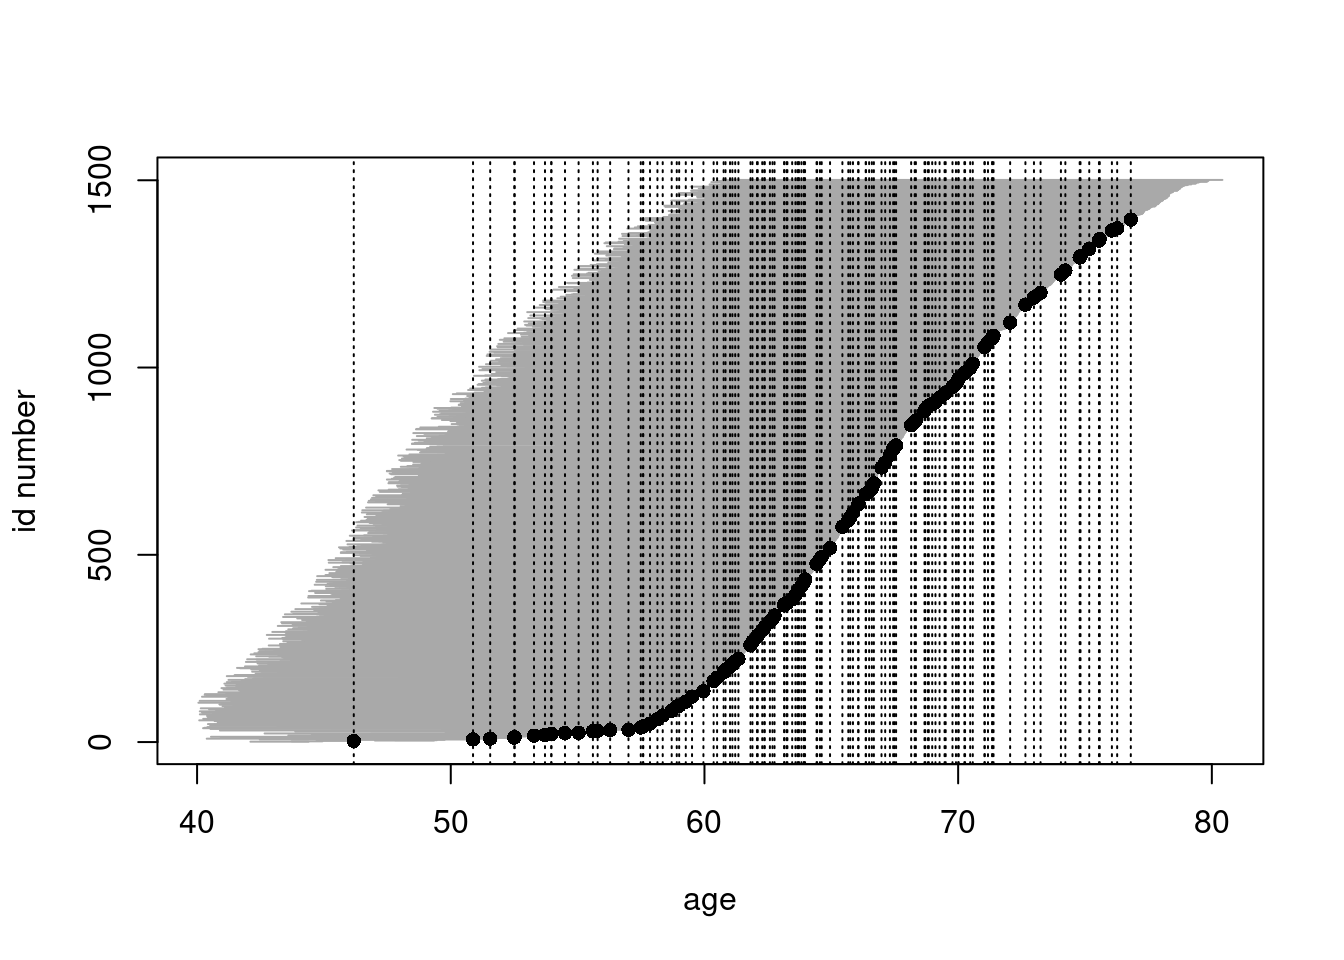
\includegraphics{occoh-caco-s_files/figure-latex/plotlexage-1.pdf}
- For a closer look, we now
zoom the graphical illustration of the risk sets into
event times occurring between 50 to 58 years. --
Copy the last four lines from the previous item and add arguments \texttt{xlim} and \texttt{ylim}
to the call of \texttt{plot()}.

\begin{Shaded}
\begin{Highlighting}[]
\FunctionTok{plot}\NormalTok{(oc.lexord, }\StringTok{"age"}\NormalTok{, }\AttributeTok{xlim =} \FunctionTok{c}\NormalTok{(}\DecValTok{50}\NormalTok{, }\DecValTok{58}\NormalTok{), }\AttributeTok{ylim =} \FunctionTok{c}\NormalTok{(}\DecValTok{5}\NormalTok{, }\DecValTok{65}\NormalTok{))}
\FunctionTok{points}\NormalTok{(}
\NormalTok{  oc.lexord, }\StringTok{"age"}\NormalTok{, }\AttributeTok{pch =} \FunctionTok{ifelse}\NormalTok{(oc.lexord}\SpecialCharTok{$}\NormalTok{lex.Xst }\SpecialCharTok{==} \DecValTok{1}\NormalTok{, }\DecValTok{16}\NormalTok{, }\ConstantTok{NA}\NormalTok{)}
\NormalTok{)}
\FunctionTok{with}\NormalTok{(}
  \FunctionTok{subset}\NormalTok{(oc.lexord, lex.Xst }\SpecialCharTok{==} \DecValTok{1}\NormalTok{),}
  \FunctionTok{abline}\NormalTok{(}\AttributeTok{v =}\NormalTok{ agexit, }\AttributeTok{lty =} \DecValTok{3}\NormalTok{)}
\NormalTok{)}
\end{Highlighting}
\end{Shaded}

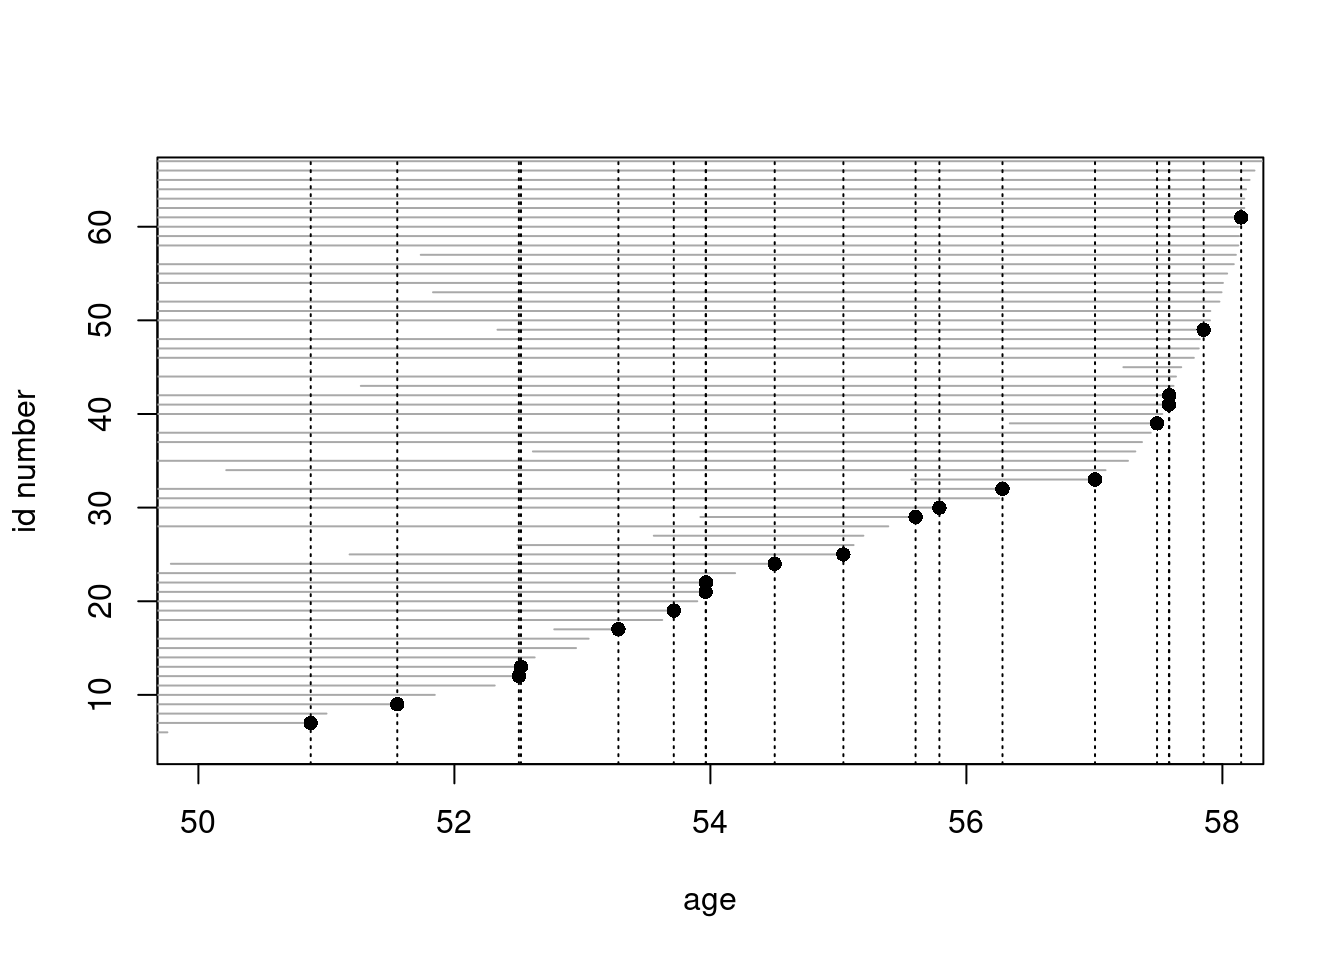
\includegraphics{occoh-caco-s_files/figure-latex/plotlexage2-1.pdf}

\section{Nested case-control study}\label{nested-case-control-study}

We shall now employ the strategy of \textbf{risk-set sampling}
or \textbf{time-matched} sampling of controls, \emph{i.e.}
we are conducting a \emph{nested case-control study}
within the cohort.

\begin{itemize}
\tightlist
\item
  The risk sets are defined according to the age at diagnosis of the case. Further matching is applied for age at entry by 1-year agebands.
  For this purpose we first generate a categorical variable
  \texttt{agen2} for age at entry
\end{itemize}

\begin{Shaded}
\begin{Highlighting}[]
\NormalTok{oc.lex}\SpecialCharTok{$}\NormalTok{agen2 }\OtherTok{\textless{}{-}} \FunctionTok{cut}\NormalTok{(oc.lex}\SpecialCharTok{$}\NormalTok{agentry, }\AttributeTok{br =} \FunctionTok{seq}\NormalTok{(}\DecValTok{40}\NormalTok{, }\DecValTok{62}\NormalTok{, }\DecValTok{1}\NormalTok{))}
\end{Highlighting}
\end{Shaded}

Matched sampling from risk sets may be carried out using
function \texttt{ccwc()} found in the \texttt{Epi} package.
Its main arguments are the times
of \texttt{entry} and \texttt{exit} which specify the time at risk along the
main time scale (here age), and the outcome variable to be given
in the \texttt{fail} argument. The number of controls per case
is set to be two, and the additional matching factor is given.
- After setting the RNG seed (with your own number),
make a call of this function and see
the structure of the resulting data frame \texttt{cactrl}
containing the cases and the chosen individual controls.

\begin{Shaded}
\begin{Highlighting}[]
\FunctionTok{set.seed}\NormalTok{(}\DecValTok{98623}\NormalTok{)}
\NormalTok{cactrl }\OtherTok{\textless{}{-}}
  \FunctionTok{ccwc}\NormalTok{(}
    \AttributeTok{entry =}\NormalTok{ agentry, }\AttributeTok{exit =}\NormalTok{ agexit, }\AttributeTok{fail =}\NormalTok{ chdeath,}
    \AttributeTok{controls =} \DecValTok{2}\NormalTok{, }\AttributeTok{match =}\NormalTok{ agen2,}
    \AttributeTok{include =} \FunctionTok{list}\NormalTok{(id, agentry),}
    \AttributeTok{data =}\NormalTok{ oc.lex, }\AttributeTok{silent =} \ConstantTok{FALSE}
\NormalTok{  )}
\end{Highlighting}
\end{Shaded}

\begin{verbatim}
## 
## Sampling risk sets: ........................................................................................................................
\end{verbatim}

\begin{Shaded}
\begin{Highlighting}[]
\FunctionTok{str}\NormalTok{(cactrl)}
\end{Highlighting}
\end{Shaded}

\begin{verbatim}
## 'data.frame':    360 obs. of  7 variables:
##  $ Set    : num  1 1 1 2 2 2 3 3 3 4 ...
##  $ Map    : num  8 1423 1 95 381 ...
##  $ Time   : num  63.9 63.9 63.9 66.7 66.7 ...
##  $ Fail   : num  1 0 0 1 0 0 1 0 0 1 ...
##  $ agen2  : Factor w/ 22 levels "(40,41]","(41,42]",..: 8 8 8 8 8 8 8 8 8 8 ...
##  $ id     : int  8 1423 1 95 381 106 115 44 1343 504 ...
##  $ agentry: num  47.7 47.9 47.5 47.5 48 ...
\end{verbatim}

Check the meaning of the four first columns of the case-control
data frame from the help page of function \texttt{ccwc()}.

\begin{itemize}
\tightlist
\item
  Now we shall start collecting data on the
  risk factors for the cases and their
  matched controls, including determination of the total cholesterol levels from the frozen sera! The storehouse of the risk factor measurements for
  the whole cohort is file \texttt{occoh-Xdata.txt}. It contains
  values of the following variables.
\end{itemize}

\begin{longtable}[]{@{}
  >{\raggedright\arraybackslash}p{(\columnwidth - 2\tabcolsep) * \real{0.1569}}
  >{\raggedright\arraybackslash}p{(\columnwidth - 2\tabcolsep) * \real{0.8431}}@{}}
\toprule\noalign{}
\begin{minipage}[b]{\linewidth}\raggedright
Variable
\end{minipage} & \begin{minipage}[b]{\linewidth}\raggedright
Description
\end{minipage} \\
\midrule\noalign{}
\endhead
\bottomrule\noalign{}
\endlastfoot
\texttt{id} & identification number, the same as in \texttt{occoh.txt} \\
\texttt{smok}. & cigarette smoking with categories; 1: \texttt{never}, 2: \texttt{former}, 3: \texttt{1-14/d}, 4: \texttt{15+/d} \\
\texttt{sbp}. & systolic blood pressure (mmHg) \\
\texttt{tchol} & total cholesterol level (mmol/l) \\
\end{longtable}

\begin{Shaded}
\begin{Highlighting}[]
\NormalTok{ocX }\OtherTok{\textless{}{-}} 
  \FunctionTok{read.table}\NormalTok{(}
    \FunctionTok{paste}\NormalTok{(url, }\StringTok{"occoh{-}Xdata.txt"}\NormalTok{, }\AttributeTok{sep =} \StringTok{"/"}\NormalTok{), }\AttributeTok{header =} \ConstantTok{TRUE}
\NormalTok{  )}
\FunctionTok{str}\NormalTok{(ocX)}
\end{Highlighting}
\end{Shaded}

\begin{verbatim}
## 'data.frame':    1501 obs. of  6 variables:
##  $ id   : int  1 2 3 4 5 6 7 8 9 10 ...
##  $ birth: chr  "1943-02-19" "1934-07-06" "1939-03-05" "1939-07-03" ...
##  $ entry: chr  "1990-08-14" "1990-08-14" "1990-08-14" "1990-08-14" ...
##  $ smok : int  4 3 3 1 2 2 1 2 1 1 ...
##  $ sbp  : int  130 128 157 102 138 119 155 154 164 124 ...
##  $ tchol: num  7.56 6.55 8.13 5.93 7.92 5.9 7.28 7.43 5.34 6.24 ...
\end{verbatim}

\begin{itemize}
\tightlist
\item
  In the next step we collect the values of the risk factors
  for our cases and controls by merging the case-control data frame and
  the storehouse file.
  In this operation we utilize function \texttt{merge()} to
  select columns of two data frames: \texttt{cactrl}
  (all columns) and \texttt{ocX} (four columns) and to merge
  these into a single file (see exercise 1.1, subsection 1.1.8, where
  \texttt{merge()} was introduced).
  The \texttt{id} variable in both files is used as the key to link each
  individual case or control with his own data on risk factors.
\end{itemize}

\begin{Shaded}
\begin{Highlighting}[]
\NormalTok{oc.ncc }\OtherTok{\textless{}{-}} \FunctionTok{merge}\NormalTok{(cactrl, ocX[, }\FunctionTok{c}\NormalTok{(}\StringTok{"id"}\NormalTok{, }\StringTok{"smok"}\NormalTok{, }\StringTok{"tchol"}\NormalTok{, }\StringTok{"sbp"}\NormalTok{)],}
  \AttributeTok{by =} \StringTok{"id"}
\NormalTok{)}
\FunctionTok{str}\NormalTok{(oc.ncc)}
\end{Highlighting}
\end{Shaded}

\begin{verbatim}
## 'data.frame':    360 obs. of  10 variables:
##  $ id     : int  1 8 10 12 14 28 37 41 41 42 ...
##  $ Set    : num  1 1 77 9 44 50 5 5 7 9 ...
##  $ Map    : num  1 8 10 12 14 28 37 41 41 42 ...
##  $ Time   : num  63.9 63.9 73 70.3 75.2 ...
##  $ Fail   : num  0 1 0 0 0 0 0 1 0 1 ...
##  $ agen2  : Factor w/ 22 levels "(40,41]","(41,42]",..: 8 8 20 17 19 19 1 1 1 17 ...
##  $ agentry: num  47.5 47.7 59.5 56.1 58.7 ...
##  $ smok   : int  4 2 1 2 4 1 3 4 4 2 ...
##  $ tchol  : num  7.56 7.43 6.24 5 3.73 4.56 5.15 6.09 6.09 5.41 ...
##  $ sbp    : int  130 154 124 148 165 230 116 125 125 156 ...
\end{verbatim}

\begin{itemize}
\tightlist
\item
  We shall treat smoking as categorical and
  total cholesterol and systolic blood pressure
  as quantitative risk factors, but the values of the
  latter will be divided by 10 to get more interpretable effect estimates.
\end{itemize}

\begin{longtable}[]{@{}
  >{\raggedright\arraybackslash}p{(\columnwidth - 2\tabcolsep) * \real{0.1569}}
  >{\raggedright\arraybackslash}p{(\columnwidth - 2\tabcolsep) * \real{0.8431}}@{}}
\toprule\noalign{}
\begin{minipage}[b]{\linewidth}\raggedright
Variable
\end{minipage} & \begin{minipage}[b]{\linewidth}\raggedright
Description
\end{minipage} \\
\midrule\noalign{}
\endhead
\bottomrule\noalign{}
\endlastfoot
\texttt{cholgrp} & cholesterol class; 1: \texttt{\textless{}5}, 2: \texttt{5-\textless{}6.5}, 3: \texttt{\textgreater{}=6.5} \\
\texttt{sbpgrp} & blood pressure class; 1: \texttt{\textless{}130}, 2: \texttt{130-\textless{}150}, 3: \texttt{150-\textless{}170}, 4: \texttt{\textgreater{}=170} \\
\end{longtable}

Convert the smoking variable into a factor.

\begin{Shaded}
\begin{Highlighting}[]
\NormalTok{oc.ncc}\SpecialCharTok{$}\NormalTok{smok }\OtherTok{\textless{}{-}} \FunctionTok{factor}\NormalTok{(oc.ncc}\SpecialCharTok{$}\NormalTok{smok,}
  \AttributeTok{labels =} \FunctionTok{c}\NormalTok{(}\StringTok{"never"}\NormalTok{, }\StringTok{"ex"}\NormalTok{, }\StringTok{"1{-}14/d"}\NormalTok{, }\StringTok{"\textgreater{}14/d"}\NormalTok{)}
\NormalTok{)}
\end{Highlighting}
\end{Shaded}

\begin{itemize}
\tightlist
\item
  It is useful to start the analysis of case-control data by
  simple tabulations by the categorized risk factors.
  Crude estimates of the rate ratios associated with them,
  in which matching is ignored, can be obtained as follows.
  We shall focus on smoking
\end{itemize}

\begin{Shaded}
\begin{Highlighting}[]
\FunctionTok{stat.table}\NormalTok{(}
  \AttributeTok{index =} \FunctionTok{list}\NormalTok{(smok, Fail),}
  \AttributeTok{contents =} \FunctionTok{list}\NormalTok{(}\FunctionTok{count}\NormalTok{(), }\FunctionTok{percent}\NormalTok{(smok)),}
  \AttributeTok{margins =} \ConstantTok{TRUE}\NormalTok{, }
  \AttributeTok{data =}\NormalTok{ oc.ncc}
\NormalTok{)}
\end{Highlighting}
\end{Shaded}

\begin{verbatim}
##  --------------------------------- 
##          ----------Fail----------- 
##  smok           0       1   Total  
##  --------------------------------- 
##  never         85      31     116  
##              35.4    25.8    32.2  
##                                    
##  ex            61      19      80  
##              25.4    15.8    22.2  
##                                    
##  1-14/d        54      42      96  
##              22.5    35.0    26.7  
##                                    
##  >14/d         40      28      68  
##              16.7    23.3    18.9  
##                                    
##                                    
##  Total        240     120     360  
##             100.0   100.0   100.0  
##  ---------------------------------
\end{verbatim}

\begin{Shaded}
\begin{Highlighting}[]
\NormalTok{smok.crncc }\OtherTok{\textless{}{-}} \FunctionTok{glm}\NormalTok{(Fail }\SpecialCharTok{\textasciitilde{}}\NormalTok{ smok, }\AttributeTok{family =}\NormalTok{ binomial, }\AttributeTok{data =}\NormalTok{ oc.ncc)}
\FunctionTok{round}\NormalTok{(}\FunctionTok{ci.exp}\NormalTok{(smok.crncc), }\DecValTok{3}\NormalTok{)}
\end{Highlighting}
\end{Shaded}

\begin{verbatim}
##             exp(Est.)  2.5% 97.5%
## (Intercept)     0.365 0.242 0.550
## smokex          0.854 0.442 1.651
## smok1-14/d      2.133 1.199 3.794
## smok>14/d       1.919 1.018 3.619
\end{verbatim}

\begin{itemize}
\tightlist
\item
  A proper analysis takes into account matching that was employed
  in the selection of controls for each case from the
  pertinent risk set, further restricted to
  subjects who were about the same age at entry as the case was.
  Also, adjustment for the other risk factors is desirable.
  In this analysis function \texttt{clogit()} in \texttt{survival} package is
  utilized. It is in fact a wrapper of function \texttt{coxph()}.
\end{itemize}

\begin{Shaded}
\begin{Highlighting}[]
\NormalTok{m.clogit }\OtherTok{\textless{}{-}} \FunctionTok{clogit}\NormalTok{(Fail }\SpecialCharTok{\textasciitilde{}}\NormalTok{ smok }\SpecialCharTok{+} \FunctionTok{I}\NormalTok{(sbp }\SpecialCharTok{/} \DecValTok{10}\NormalTok{) }\SpecialCharTok{+}\NormalTok{ tchol }\SpecialCharTok{+}
  \FunctionTok{strata}\NormalTok{(Set), }\AttributeTok{data =}\NormalTok{ oc.ncc)}
\FunctionTok{summary}\NormalTok{(m.clogit)}
\end{Highlighting}
\end{Shaded}

\begin{verbatim}
## Call:
## coxph(formula = Surv(rep(1, 360L), Fail) ~ smok + I(sbp/10) + 
##     tchol + strata(Set), data = oc.ncc, method = "exact")
## 
##   n= 360, number of events= 120 
## 
##                coef exp(coef) se(coef)      z Pr(>|z|)    
## smokex     -0.22100   0.80172  0.35085 -0.630  0.52877    
## smok1-14/d  0.59186   1.80734  0.29894  1.980  0.04772 *  
## smok>14/d   0.56616   1.76149  0.33326  1.699  0.08935 .  
## I(sbp/10)   0.11171   1.11818  0.05453  2.049  0.04050 *  
## tchol       0.40091   1.49319  0.11142  3.598  0.00032 ***
## ---
## Signif. codes:  0 '***' 0.001 '**' 0.01 '*' 0.05 '.' 0.1 ' ' 1
## 
##            exp(coef) exp(-coef) lower .95 upper .95
## smokex        0.8017     1.2473    0.4031     1.595
## smok1-14/d    1.8073     0.5533    1.0060     3.247
## smok>14/d     1.7615     0.5677    0.9167     3.385
## I(sbp/10)     1.1182     0.8943    1.0048     1.244
## tchol         1.4932     0.6697    1.2003     1.858
## 
## Concordance= 0.679  (se = 0.046 )
## Likelihood ratio test= 28.81  on 5 df,   p=3e-05
## Wald test            = 24.31  on 5 df,   p=2e-04
## Score (logrank) test = 27.31  on 5 df,   p=5e-05
\end{verbatim}

\begin{Shaded}
\begin{Highlighting}[]
\FunctionTok{round}\NormalTok{(}\FunctionTok{ci.exp}\NormalTok{(m.clogit), }\DecValTok{3}\NormalTok{)}
\end{Highlighting}
\end{Shaded}

\begin{verbatim}
##            exp(Est.)  2.5% 97.5%
## smokex         0.802 0.403 1.595
## smok1-14/d     1.807 1.006 3.247
## smok>14/d      1.761 0.917 3.385
## I(sbp/10)      1.118 1.005 1.244
## tchol          1.493 1.200 1.858
\end{verbatim}

Compare these with the crude estimates obtained above.

\section{Case-cohort study}\label{case-cohort-study}

Now we start applying the second major outcome-selective
sampling strategy
for collecting exposure data from a big study population

\begin{itemize}
\tightlist
\item
  The subcohort is selected as a\\
  simple random sample (\(n=260\)) from the whole cohort.
  The \texttt{id}-numbers of the individuals that are
  selected will be stored in vector \texttt{subcids}, and
  \texttt{subcind} is an indicator for inclusion to the subcohort.
\end{itemize}

\begin{Shaded}
\begin{Highlighting}[]
\NormalTok{N }\OtherTok{\textless{}{-}} \DecValTok{1501}
\NormalTok{n }\OtherTok{\textless{}{-}} \DecValTok{260}
\FunctionTok{set.seed}\NormalTok{(}\DecValTok{15792}\NormalTok{)}
\NormalTok{subcids }\OtherTok{\textless{}{-}} \FunctionTok{sample}\NormalTok{(N, n)}
\NormalTok{oc.lexord}\SpecialCharTok{$}\NormalTok{subcind }\OtherTok{\textless{}{-}} \DecValTok{1} \SpecialCharTok{*}\NormalTok{ (oc.lexord}\SpecialCharTok{$}\NormalTok{id }\SpecialCharTok{\%in\%}\NormalTok{ subcids)}
\end{Highlighting}
\end{Shaded}

\begin{itemize}
\tightlist
\item
  We form the data frame \texttt{oc.cc}
  to be used in the subsequent
  analysis selecting the union of the subcohort members
  and the case group from the data frame of the full cohort.
  After that we collect the data of the risk factors from the
  data storehouse for the subjects in the case-cohort data
\end{itemize}

\begin{Shaded}
\begin{Highlighting}[]
\NormalTok{oc.cc }\OtherTok{\textless{}{-}} \FunctionTok{subset}\NormalTok{(oc.lexord, subcind }\SpecialCharTok{==} \DecValTok{1} \SpecialCharTok{|}\NormalTok{ chdeath }\SpecialCharTok{==} \DecValTok{1}\NormalTok{)}
\NormalTok{oc.cc }\OtherTok{\textless{}{-}} \FunctionTok{merge}\NormalTok{(oc.cc, ocX[, }\FunctionTok{c}\NormalTok{(}\StringTok{"id"}\NormalTok{, }\StringTok{"smok"}\NormalTok{, }\StringTok{"tchol"}\NormalTok{, }\StringTok{"sbp"}\NormalTok{)],}
  \AttributeTok{by =} \StringTok{"id"}
\NormalTok{)}
\FunctionTok{str}\NormalTok{(oc.cc)}
\end{Highlighting}
\end{Shaded}

\begin{verbatim}
## Classes 'Lexis' and 'data.frame':    362 obs. of  21 variables:
##  $ id     : int  8 10 34 40 41 42 43 45 51 62 ...
##  $ age    : num  47.7 59.5 51.9 45.2 40.2 ...
##  $ lex.dur: num  16.21 19.38 19.36 4.59 19.32 ...
##  $ lex.Cst: num  0 0 0 0 0 0 0 0 0 0 ...
##  $ lex.Xst: int  1 0 0 0 1 1 1 0 1 1 ...
##  $ lex.id : int  430 1483 1074 6 121 987 746 486 1056 663 ...
##  $ ID     : int  430 1483 1074 6 121 987 746 486 1056 663 ...
##  $ birth  : chr  "1942-11-24" "1931-03-01" "1938-09-14" "1945-06-22" ...
##  $ entry  : chr  "1990-08-15" "1990-08-15" "1990-08-20" "1990-08-21" ...
##  $ exit   : chr  "2006-10-30" "2009-12-31" "2009-12-31" "1995-03-26" ...
##  $ death  : int  1 0 0 1 1 1 1 0 1 1 ...
##  $ chdeath: int  1 0 0 0 1 1 1 0 1 1 ...
##  $ ybirth : num  1943 1931 1939 1945 1950 ...
##  $ yentry : num  1991 1991 1991 1991 1991 ...
##  $ yexit  : num  2007 2010 2010 1995 2010 ...
##  $ agentry: num  47.7 59.5 51.9 45.2 40.2 ...
##  $ agexit : num  63.9 78.8 71.3 49.8 59.5 ...
##  $ subcind: num  0 1 1 1 0 0 0 1 1 0 ...
##  $ smok   : int  2 1 1 4 4 2 3 2 1 2 ...
##  $ tchol  : num  7.43 6.24 5.8 5.88 6.09 5.41 5.72 5.98 7.12 5.57 ...
##  $ sbp    : int  154 124 113 141 125 156 128 115 137 173 ...
##  - attr(*, "breaks")=List of 1
##   ..$ age: NULL
##  - attr(*, "time.scales")= chr "age"
##  - attr(*, "time.since")= chr ""
\end{verbatim}

\begin{itemize}
\tightlist
\item
  We shall now create a graphical illustration of
  the lifelines contained in the case-cohort data.
  Lines for the subcohort non-cases are grey without bullet at exit,
  those for subcohort cases are blue with blue bullet at exit, and
  for cases outside the subcohort the lines are red and dotted with
  red bullets at exit.
\end{itemize}

\begin{Shaded}
\begin{Highlighting}[]
\FunctionTok{plot}\NormalTok{(}\FunctionTok{subset}\NormalTok{(oc.cc, chdeath }\SpecialCharTok{==} \DecValTok{0}\NormalTok{), }\StringTok{"age"}\NormalTok{)}
\FunctionTok{lines}\NormalTok{(}\FunctionTok{subset}\NormalTok{(oc.cc, chdeath }\SpecialCharTok{==} \DecValTok{1} \SpecialCharTok{\&}\NormalTok{ subcind }\SpecialCharTok{==} \DecValTok{1}\NormalTok{), }\AttributeTok{col =} \StringTok{"blue"}\NormalTok{)}
\FunctionTok{lines}\NormalTok{(}\FunctionTok{subset}\NormalTok{(oc.cc, chdeath }\SpecialCharTok{==} \DecValTok{1} \SpecialCharTok{\&}\NormalTok{ subcind }\SpecialCharTok{==} \DecValTok{0}\NormalTok{), }\AttributeTok{col =} \StringTok{"red"}\NormalTok{)}
\FunctionTok{points}\NormalTok{(}\FunctionTok{subset}\NormalTok{(oc.cc, chdeath }\SpecialCharTok{==} \DecValTok{1}\NormalTok{),}
  \AttributeTok{pch =} \DecValTok{16}\NormalTok{,}
  \AttributeTok{col =} \FunctionTok{c}\NormalTok{(}\StringTok{"blue"}\NormalTok{, }\StringTok{"red"}\NormalTok{)[oc.cc}\SpecialCharTok{$}\NormalTok{subcind }\SpecialCharTok{+} \DecValTok{1}\NormalTok{]}
\NormalTok{)}
\end{Highlighting}
\end{Shaded}

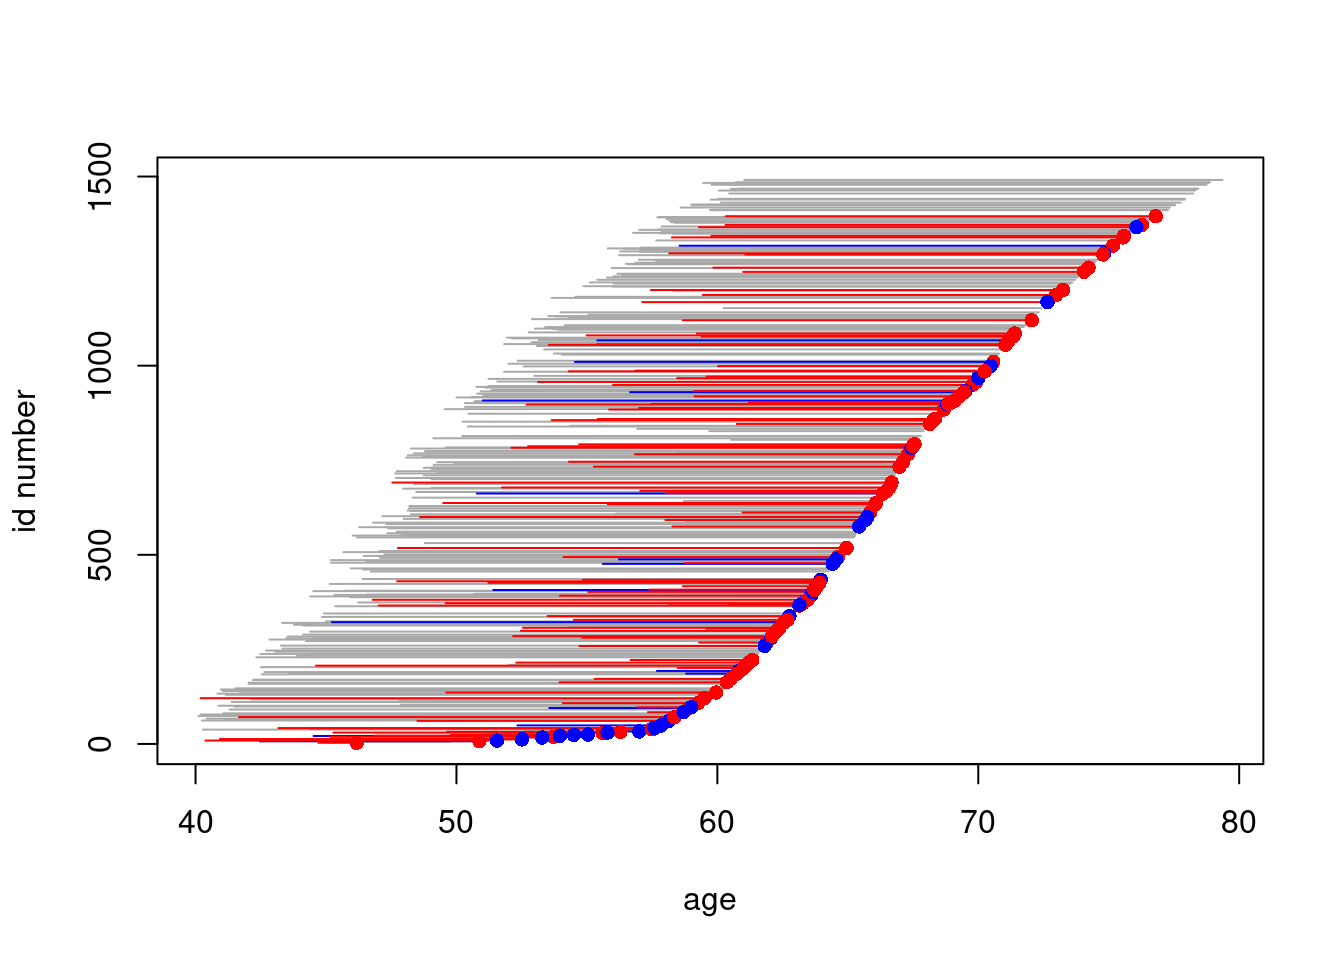
\includegraphics{occoh-caco-s_files/figure-latex/casecoh-lines-1.pdf}

\begin{itemize}
\tightlist
\item
  Define the categorical smoking variable again.
\end{itemize}

\begin{Shaded}
\begin{Highlighting}[]
\NormalTok{oc.cc}\SpecialCharTok{$}\NormalTok{smok }\OtherTok{\textless{}{-}} \FunctionTok{factor}\NormalTok{(oc.cc}\SpecialCharTok{$}\NormalTok{smok,}
  \AttributeTok{labels =} \FunctionTok{c}\NormalTok{(}\StringTok{"never"}\NormalTok{, }\StringTok{"ex"}\NormalTok{, }\StringTok{"1{-}14/d"}\NormalTok{, }\StringTok{"\textgreater{}14/d"}\NormalTok{)}
\NormalTok{)}
\end{Highlighting}
\end{Shaded}

A crude estimate of the hazard ratio for the various smoking categories \(k\)
vs.~non-smokers (\(k=1\)) can be obtained by tabulating cases \((D_k)\) and person-years (\(y_k\))
in the subcohort by smoking and then computing the
relevant exposure odds ratio for each category:
\[ \text{HR}_k ^{\text{crude}} = \frac{D_k/D_1}{y_k/y_1} \]

\begin{Shaded}
\begin{Highlighting}[]
\NormalTok{sm.cc }\OtherTok{\textless{}{-}} \FunctionTok{stat.table}\NormalTok{(}
  \AttributeTok{index =}\NormalTok{ smok,}
  \AttributeTok{contents =} \FunctionTok{list}\NormalTok{(}\AttributeTok{Cases =} \FunctionTok{sum}\NormalTok{(lex.Xst), }\AttributeTok{Pyrs =} \FunctionTok{sum}\NormalTok{(lex.dur)),}
  \AttributeTok{margins =} \ConstantTok{TRUE}\NormalTok{, }
  \AttributeTok{data =}\NormalTok{ oc.cc}
\NormalTok{)}
\FunctionTok{print}\NormalTok{(sm.cc, }\AttributeTok{digits =} \FunctionTok{c}\NormalTok{(}\AttributeTok{sum =} \DecValTok{0}\NormalTok{, }\AttributeTok{ratio =} \DecValTok{1}\NormalTok{))}
\end{Highlighting}
\end{Shaded}

\begin{verbatim}
##  ------------------------- 
##  smok       Cases    Pyrs  
##  ------------------------- 
##  never         31    2071  
##  ex            19    1174  
##  1-14/d        42    1399  
##  >14/d         28     846  
##                            
##  Total        120    5489  
##  -------------------------
\end{verbatim}

\begin{Shaded}
\begin{Highlighting}[]
\NormalTok{HRcc }\OtherTok{\textless{}{-}} 
\NormalTok{  (sm.cc[}\DecValTok{1}\NormalTok{, }\SpecialCharTok{{-}}\DecValTok{5}\NormalTok{] }\SpecialCharTok{/}\NormalTok{ sm.cc[}\DecValTok{1}\NormalTok{, }\DecValTok{1}\NormalTok{]) }\SpecialCharTok{/}\NormalTok{ (sm.cc[}\DecValTok{2}\NormalTok{, }\SpecialCharTok{{-}}\DecValTok{5}\NormalTok{] }\SpecialCharTok{/}\NormalTok{ sm.cc[}\DecValTok{2}\NormalTok{, }\DecValTok{1}\NormalTok{])}
\FunctionTok{round}\NormalTok{(HRcc, }\DecValTok{3}\NormalTok{)}
\end{Highlighting}
\end{Shaded}

\begin{verbatim}
##  never     ex 1-14/d  >14/d 
##  1.000  1.081  2.006  2.211
\end{verbatim}

\section{Do these estimates resemble those obtained from nested case-control data?}\label{do-these-estimates-resemble-those-obtained-from-nested-case-control-data}

To estimate the rate ratios associated with smoking and adjusted for the
other risk factors we now fit the pertinent Cox model
applying the method of \emph{weighted partial likelihood} as
presented by Ling \& Ying (1993) and Barlow (1994).
This analysis can be done using function \texttt{cch()}
in package \texttt{survival} with \texttt{method\ =\ "LinYing"}

\begin{Shaded}
\begin{Highlighting}[]
\NormalTok{oc.cc}\SpecialCharTok{$}\NormalTok{survobj }\OtherTok{\textless{}{-}} \FunctionTok{with}\NormalTok{(oc.cc, }\FunctionTok{Surv}\NormalTok{(agentry, agexit, chdeath))}
\NormalTok{cch.LY }\OtherTok{\textless{}{-}} \FunctionTok{cch}\NormalTok{(survobj }\SpecialCharTok{\textasciitilde{}}\NormalTok{ smok }\SpecialCharTok{+} \FunctionTok{I}\NormalTok{(sbp }\SpecialCharTok{/} \DecValTok{10}\NormalTok{) }\SpecialCharTok{+}\NormalTok{ tchol,}
  \AttributeTok{stratum =} \ConstantTok{NULL}\NormalTok{,}
  \AttributeTok{subcoh =} \SpecialCharTok{\textasciitilde{}}\NormalTok{subcind, }\AttributeTok{id =} \SpecialCharTok{\textasciitilde{}}\NormalTok{id, }\AttributeTok{cohort.size =}\NormalTok{ N, }\AttributeTok{data =}\NormalTok{ oc.cc,}
  \AttributeTok{method =} \StringTok{"LinYing"}
\NormalTok{)}
\FunctionTok{summary}\NormalTok{(cch.LY)}
\end{Highlighting}
\end{Shaded}

\begin{verbatim}
## Case-cohort analysis,x$method, LinYing 
##  with subcohort of 260 from cohort of 1501 
## 
## Call: cch(formula = survobj ~ smok + I(sbp/10) + tchol, data = oc.cc, 
##     subcoh = ~subcind, id = ~id, stratum = NULL, cohort.size = N, 
##     method = "LinYing")
## 
## Coefficients:
##              Coef    HR  (95%   CI)     p
## smokex     -0.096 0.909 0.457 1.806 0.785
## smok1-14/d  0.769 2.157 1.180 3.943 0.012
## smok>14/d   1.085 2.959 1.532 5.718 0.001
## I(sbp/10)   0.218 1.244 1.119 1.383 0.000
## tchol       0.350 1.419 1.152 1.748 0.001
\end{verbatim}

\section{Full cohort analysis and comparisons}\label{full-cohort-analysis-and-comparisons}

Finally, suppose the investigators after all could afford to collect the
data on risk factors from the storehouse for the whole cohort.

\begin{itemize}
\tightlist
\item
  Let us form the data frame corresponding to the full cohort design
  and convert again smoking to be categorical.
\end{itemize}

\begin{Shaded}
\begin{Highlighting}[]
\NormalTok{oc.full }\OtherTok{\textless{}{-}} \FunctionTok{merge}\NormalTok{(oc.lex, ocX[, }\FunctionTok{c}\NormalTok{(}\StringTok{"id"}\NormalTok{, }\StringTok{"smok"}\NormalTok{, }\StringTok{"tchol"}\NormalTok{, }\StringTok{"sbp"}\NormalTok{)],}
  \AttributeTok{by.x =} \StringTok{"id"}\NormalTok{, }\AttributeTok{by.y =} \StringTok{"id"}
\NormalTok{)}
\NormalTok{oc.full}\SpecialCharTok{$}\NormalTok{smok }\OtherTok{\textless{}{-}} \FunctionTok{factor}\NormalTok{(oc.full}\SpecialCharTok{$}\NormalTok{smok,}
  \AttributeTok{labels =} \FunctionTok{c}\NormalTok{(}\StringTok{"never"}\NormalTok{, }\StringTok{"ex"}\NormalTok{, }\StringTok{"1{-}14/d"}\NormalTok{, }\StringTok{"\textgreater{}14/d"}\NormalTok{)}
\NormalTok{)}
\end{Highlighting}
\end{Shaded}

Juts for comparison with the corresponding analysis in case-cohort data
perform a similar crude estimation of hazard ratios associated with smoking.

\begin{Shaded}
\begin{Highlighting}[]
\NormalTok{sm.coh }\OtherTok{\textless{}{-}} \FunctionTok{stat.table}\NormalTok{(}
  \AttributeTok{index =}\NormalTok{ smok,}
  \AttributeTok{contents =} \FunctionTok{list}\NormalTok{(}\AttributeTok{Cases =} \FunctionTok{sum}\NormalTok{(lex.Xst), }\AttributeTok{Pyrs =} \FunctionTok{sum}\NormalTok{(lex.dur)),}
  \AttributeTok{margins =} \ConstantTok{TRUE}\NormalTok{, }
  \AttributeTok{data =}\NormalTok{ oc.full}
\NormalTok{)}
\FunctionTok{print}\NormalTok{(sm.coh, }\AttributeTok{digits =} \FunctionTok{c}\NormalTok{(}\AttributeTok{sum =} \DecValTok{0}\NormalTok{, }\AttributeTok{ratio =} \DecValTok{1}\NormalTok{))}
\end{Highlighting}
\end{Shaded}

\begin{verbatim}
##  ------------------------- 
##  smok       Cases    Pyrs  
##  ------------------------- 
##  never         31   10363  
##  ex            19    4879  
##  1-14/d        42    6246  
##  >14/d         28    3793  
##                            
##  Total        120   25281  
##  -------------------------
\end{verbatim}

\begin{Shaded}
\begin{Highlighting}[]
\NormalTok{HRcoh }\OtherTok{\textless{}{-}} 
\NormalTok{  (sm.coh[}\DecValTok{1}\NormalTok{, }\SpecialCharTok{{-}}\DecValTok{5}\NormalTok{] }\SpecialCharTok{/}\NormalTok{ sm.coh[}\DecValTok{1}\NormalTok{, }\DecValTok{1}\NormalTok{]) }\SpecialCharTok{/}\NormalTok{ (sm.coh[}\DecValTok{2}\NormalTok{, }\SpecialCharTok{{-}}\DecValTok{5}\NormalTok{] }\SpecialCharTok{/}\NormalTok{ sm.coh[}\DecValTok{2}\NormalTok{, }\DecValTok{1}\NormalTok{])}
\FunctionTok{round}\NormalTok{(HRcoh, }\DecValTok{3}\NormalTok{)}
\end{Highlighting}
\end{Shaded}

\begin{verbatim}
##  never     ex 1-14/d  >14/d 
##  1.000  1.302  2.248  2.468
\end{verbatim}

\begin{itemize}
\tightlist
\item
  Fit now the ordinary Cox model to the full cohort. There is no need
  to employ extra tricks upon the ordinary \texttt{coxph()} fit.
\end{itemize}

\begin{Shaded}
\begin{Highlighting}[]
\NormalTok{cox.coh }\OtherTok{\textless{}{-}} \FunctionTok{coxph}\NormalTok{(}\FunctionTok{Surv}\NormalTok{(agentry, agexit, chdeath) }\SpecialCharTok{\textasciitilde{}}
\NormalTok{  smok }\SpecialCharTok{+} \FunctionTok{I}\NormalTok{(sbp }\SpecialCharTok{/} \DecValTok{10}\NormalTok{) }\SpecialCharTok{+}\NormalTok{ tchol, }\AttributeTok{data =}\NormalTok{ oc.full)}
\FunctionTok{summary}\NormalTok{(cox.coh)}
\end{Highlighting}
\end{Shaded}

\begin{verbatim}
## Call:
## coxph(formula = Surv(agentry, agexit, chdeath) ~ smok + I(sbp/10) + 
##     tchol, data = oc.full)
## 
##   n= 1501, number of events= 120 
## 
##               coef exp(coef) se(coef)     z Pr(>|z|)    
## smokex     0.10955   1.11577  0.29240 0.375 0.707922    
## smok1-14/d 0.72567   2.06612  0.23704 3.061 0.002203 ** 
## smok>14/d  0.95054   2.58711  0.26198 3.628 0.000285 ***
## I(sbp/10)  0.14372   1.15456  0.04096 3.509 0.000450 ***
## tchol      0.26517   1.30366  0.07089 3.740 0.000184 ***
## ---
## Signif. codes:  0 '***' 0.001 '**' 0.01 '*' 0.05 '.' 0.1 ' ' 1
## 
##            exp(coef) exp(-coef) lower .95 upper .95
## smokex         1.116     0.8962     0.629     1.979
## smok1-14/d     2.066     0.4840     1.298     3.288
## smok>14/d      2.587     0.3865     1.548     4.323
## I(sbp/10)      1.155     0.8661     1.065     1.251
## tchol          1.304     0.7671     1.135     1.498
## 
## Concordance= 0.681  (se = 0.026 )
## Likelihood ratio test= 41.16  on 5 df,   p=9e-08
## Wald test            = 42.05  on 5 df,   p=6e-08
## Score (logrank) test = 43.29  on 5 df,   p=3e-08
\end{verbatim}

\begin{itemize}
\tightlist
\item
  Lastly, a comparison of the point estimates and standard errors between
  the different designs, including variants of analysis for the case-cohort design, can be performed.
\end{itemize}

\begin{Shaded}
\begin{Highlighting}[]
\NormalTok{betas }\OtherTok{\textless{}{-}} \FunctionTok{cbind}\NormalTok{(}\FunctionTok{coef}\NormalTok{(cox.coh), }\FunctionTok{coef}\NormalTok{(m.clogit), }\FunctionTok{coef}\NormalTok{(cch.LY))}
\FunctionTok{colnames}\NormalTok{(betas) }\OtherTok{\textless{}{-}} \FunctionTok{c}\NormalTok{(}\StringTok{"coh"}\NormalTok{, }\StringTok{"ncc"}\NormalTok{, }\StringTok{"cch.LY"}\NormalTok{)}
\FunctionTok{round}\NormalTok{(betas, }\DecValTok{3}\NormalTok{)}
\end{Highlighting}
\end{Shaded}

\begin{verbatim}
##              coh    ncc cch.LY
## smokex     0.110 -0.221 -0.096
## smok1-14/d 0.726  0.592  0.769
## smok>14/d  0.951  0.566  1.085
## I(sbp/10)  0.144  0.112  0.218
## tchol      0.265  0.401  0.350
\end{verbatim}

\begin{Shaded}
\begin{Highlighting}[]
\NormalTok{SEs }\OtherTok{\textless{}{-}} \FunctionTok{cbind}\NormalTok{(}
  \FunctionTok{sqrt}\NormalTok{(}\FunctionTok{diag}\NormalTok{(cox.coh}\SpecialCharTok{$}\NormalTok{var)),}
  \FunctionTok{sqrt}\NormalTok{(}\FunctionTok{diag}\NormalTok{(m.clogit}\SpecialCharTok{$}\NormalTok{var)),}
  \FunctionTok{sqrt}\NormalTok{(}\FunctionTok{diag}\NormalTok{(cch.LY}\SpecialCharTok{$}\NormalTok{var))}
\NormalTok{)}
\FunctionTok{colnames}\NormalTok{(SEs) }\OtherTok{\textless{}{-}} \FunctionTok{colnames}\NormalTok{(betas)}
\FunctionTok{round}\NormalTok{(SEs, }\DecValTok{3}\NormalTok{)}
\end{Highlighting}
\end{Shaded}

\begin{verbatim}
##              coh   ncc cch.LY
## smokex     0.292 0.351  0.350
## smok1-14/d 0.237 0.299  0.308
## smok>14/d  0.262 0.333  0.336
## I(sbp/10)  0.041 0.055  0.054
## tchol      0.071 0.111  0.106
\end{verbatim}

You will notice that the point estimates of the coefficients
obtained from the full cohort, nested case-control, and case-cohort analyses,
respectively, are somewhat variable. However,\\
the standard errors from the NCC and CC
analyses should be quite similar when the numbers of cases and non-cases are similar.

\section{Further exercises and homework}\label{further-exercises-and-homework}

\begin{itemize}
\item
  If you have time, you could run both the NCC study and CC study
  again but now with a larger control group or subcohort;
  for example 4 controls per case in NCC and \(n=520\) as the subcohort size in CC.
  Remember resetting the seed first.
  Pay attention in the results to how much closer
  will be the point estimates and the proper SEs to those
  obtained from the full cohort design.
\item
  Instead of simple linear terms for \texttt{sbp} and \texttt{tchol} you could try to fit
  spline models to describe their effects.
\item
  A popular alternative to weighted partial likelihood
  in the analysis of case-cohort data is the \emph{pseudo-likelihood method}
  (Prentice 1986), which is based on \emph{late entry} to follow-up
  of the case subjects not belonging to
  the subcohort.
  The way to do this is provided by function \texttt{cch()} which
  you can apply directly to the case-cohort data \texttt{oc.cc} as before
  but now with \texttt{method\ =\ "Prentice"}. -- Try this and compare the results
  with those obtained by weighted partial likelihood in model
  \texttt{cch.LY}.
\item
  Yet another computational solution for
  maximizing weighted partial likelihood is provided by
  a combination of functions \texttt{twophase()}
  and \texttt{svycoxph()} of the \texttt{survey} package.
  The approach is illustrated with an example
  in a vignette \emph{Two-phase designs in epidemiology} by Thomas Lumley
  (see \url{http://cran.r-project.org/web/packages/survey/vignettes/epi.pdf}).
  -- You can try this at home and check that you would obtain similar results as
  with model \texttt{cch.LY}.
\end{itemize}

\chapter{Causal inference 2: Model-based estimation of causal estimands}\label{causal-inference-2-model-based-estimation-of-causal-estimands}

Sources of inspiration: \href{https://doi.org/10.1002/sim.7628}{Luque Fernandez, M.A.~et al.
(2018)} \emph{Stat Med}
2018;37(16):2530-2546 and\\
\href{https://doi.org/10.1002/sim.9234}{Smith et al.~(2022)} \emph{Stat Med}
2022;41(2):407-432.

We shall illustrate with simulated data the estimation of causal effects
of a binary exposure \(X\) when the outcome \(Y\) is also binary, and there
is a set of four covariates \(Z = (Z_1, Z_2, Z_3, Z_4)\). As a background
story, we imagine a population of cancer patients, in whom the variables
and the assumed marginal distributions of the covariates are

\begin{longtable}[]{@{}
  >{\raggedright\arraybackslash}p{(\columnwidth - 2\tabcolsep) * \real{0.2113}}
  >{\raggedright\arraybackslash}p{(\columnwidth - 2\tabcolsep) * \real{0.7887}}@{}}
\toprule\noalign{}
\begin{minipage}[b]{\linewidth}\raggedright
Variable
\end{minipage} & \begin{minipage}[b]{\linewidth}\raggedright
Description
\end{minipage} \\
\midrule\noalign{}
\endhead
\bottomrule\noalign{}
\endlastfoot
\(X\) & treatment; 1: radiotherapy only, 0: radiotherapy + chemotherapy \\
\(Y\) & death during one year after diagnosis of cancer \\
\(Z_1\) & sex; 0: man, 1: woman; \(Z_1 \sim \text{Bern}(0.5)\) \\
\(Z_2\) & age group 0; \texttt{young}, 1: \texttt{old}; \(Z_2 \sim \text{Bern}(0.65)\) \\
\(Z_3\) & stage of cancer; 4 classes; \(Z_3 \sim \text{DiscUnif}(1, \dots, 4)\) \\
\(Z_4\) & comorbidity score; 5 classes; \(Z_3 \sim \text{DiscUnif}(1, \dots, 5)\) \\
\end{longtable}

For simplicity, covariates \(Z_3\) and \(Z_4\) are treated as continuous
variables in the models. The assumed causal diagram is shown below.

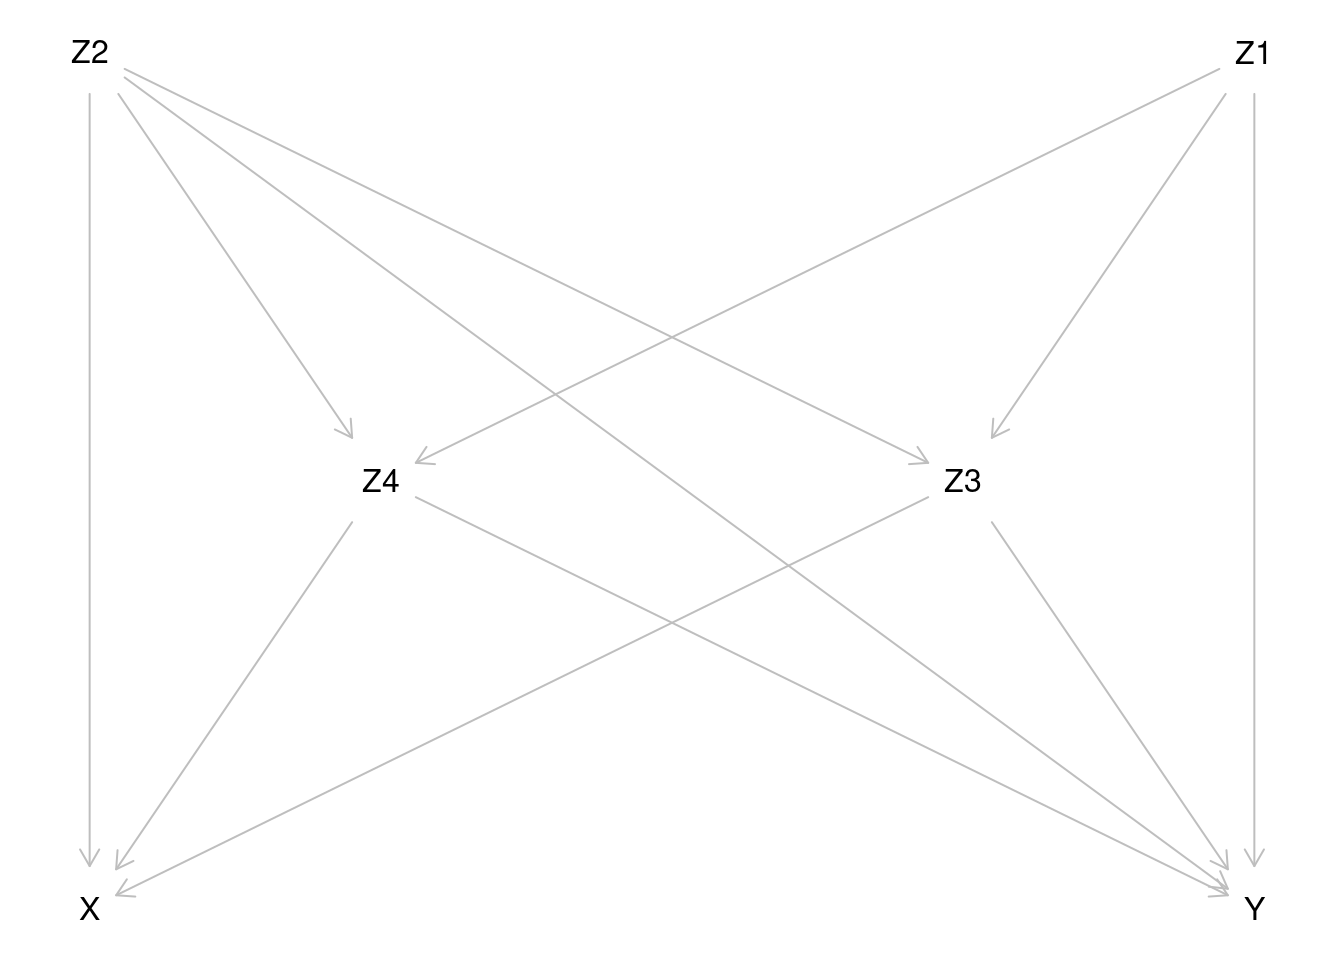
\includegraphics{causInf2-s_files/figure-latex/unnamed-chunk-2-1.pdf}

For more generic notation, the probabilities of \(Y=1\) will be expressed
as expectations, e.g.~\(E(Y^{X=x}) = P(Y^{X=x}=1)\) and
\(E(Y|X=x, Z=z) = P(Y=1|X=x, Z=z)\), where \(Z\) is the vector of relevant
covariates. The same principle is applied in expressing the conditional
probability of \(X=1\) given \(Z=z\). The fitted or predicted probabilities
of \(Y=1\) are denoted as fitted \(\widehat{Y}\) or predicted values
\(\widetilde{Y}\) of \(Y\) with pertinent subscripts and/or superscripts.
Both \(X\) and \(Y\) are modelled by logistic regression. The expit-function
or inverse of the logit function is defined:
\(\text{expit}(u) = 1/(1 + e^{-u})\), \(u\in R\). This is equal to the
cumulative distribution function of the standard logistic distribution,
the values of which are returned in R by \texttt{plogis(u)}. The R function
that returns values of the logit-function is \texttt{qlogis()}.

The true model assumed for the dependence of exposure \(X\) on covariates:
\[ E(X|Z_1 = z_1, \dots, Z_4 = z_4) =
      \text{expit}(-5 + 0.05z_2 + 0.25z_3 + 0.5z_4 + 0.4z_2z_4) . \] The
assumed true model for the outcome is
\[ E(Y|X=x, Z_1 = z_1, \dots, Z_4 = z_4) =
           \text{expit}(-1 + x - 0.1z_1 + 0.35z_2 + 0.25z_3 +
                 0.20z_4 + 0.15z_2z_4) \] Note that \(X\) does not depend
on \(Z_1\), and that in both models there is a product term \(Z_2 Z_4\),
which appears weaker for the outcome model.

\section{Control of confounding}\label{control-of-confounding}

\begin{enumerate}
\def\labelenumi{\arabic{enumi}.}
\item
  Based on inspection of the causal diagram, can you provide
  justification for the claim that variables \(Z_2, Z_3\) and \(Z_4\) form
  a proper subset of the four covariates, which is sufficient to block
  all backdoor paths between \(X\) and \(Y\) and thus remove confounding?
\item
  Even though we have such a minimal sufficient set as indicated in
  item (a), why could it still be worth while to include covariate
  \(Z_1\), too, when modelling the outcome?
\end{enumerate}

\section{Generation of target population and true models}\label{generation-of-target-population-and-true-models}

\begin{enumerate}
\def\labelenumi{\arabic{enumi}.}
\tightlist
\item
  Load the necessary packages.
\end{enumerate}

\begin{Shaded}
\begin{Highlighting}[]
\FunctionTok{library}\NormalTok{(Epi)}
\FunctionTok{library}\NormalTok{(stdReg)}
\FunctionTok{library}\NormalTok{(PSweight)}
\FunctionTok{library}\NormalTok{(SuperLearner)}
\end{Highlighting}
\end{Shaded}

\begin{verbatim}
## Loading required package: nnls
\end{verbatim}

\begin{verbatim}
## Loading required package: gam
\end{verbatim}

\begin{verbatim}
## Loading required package: splines
\end{verbatim}

\begin{verbatim}
## Loading required package: foreach
\end{verbatim}

\begin{verbatim}
## Loaded gam 1.22-3
\end{verbatim}

\begin{verbatim}
## Super Learner
\end{verbatim}

\begin{verbatim}
## Version: 2.0-29
\end{verbatim}

\begin{verbatim}
## Package created on 2024-02-06
\end{verbatim}

\begin{Shaded}
\begin{Highlighting}[]
\FunctionTok{library}\NormalTok{(tmle)}
\end{Highlighting}
\end{Shaded}

\begin{verbatim}
## Loading required package: glmnet
\end{verbatim}

\begin{verbatim}
## Loading required package: Matrix
\end{verbatim}

\begin{verbatim}
## Loaded glmnet 4.1-8
\end{verbatim}

\begin{verbatim}
## Welcome to the tmle package, version 2.0.1
## 
## Use tmleNews() to see details on changes and bug fixes
\end{verbatim}

\begin{enumerate}
\def\labelenumi{\arabic{enumi}.}
\setcounter{enumi}{1}
\tightlist
\item
  Define the R-functions which computes expected values for the
  exposure and outcome based on the assumed true outcome model and the
  true exposure model.
\end{enumerate}

\begin{Shaded}
\begin{Highlighting}[]
\NormalTok{EX }\OtherTok{\textless{}{-}} \ControlFlowTok{function}\NormalTok{(z2, z3, z4) \{}
  \FunctionTok{plogis}\NormalTok{(}\SpecialCharTok{{-}}\DecValTok{5} \SpecialCharTok{+} \FloatTok{0.05} \SpecialCharTok{*}\NormalTok{ z2 }\SpecialCharTok{+} \FloatTok{0.25} \SpecialCharTok{*}\NormalTok{ z3 }\SpecialCharTok{+} \FloatTok{0.5} \SpecialCharTok{*}\NormalTok{ z4 }\SpecialCharTok{+} \FloatTok{0.4} \SpecialCharTok{*}\NormalTok{ z2 }\SpecialCharTok{*}\NormalTok{ z4)}
\NormalTok{\}}
\NormalTok{EY }\OtherTok{\textless{}{-}} \ControlFlowTok{function}\NormalTok{(x, z1, z2, z3, z4) \{}
  \FunctionTok{plogis}\NormalTok{(}\SpecialCharTok{{-}}\DecValTok{1} \SpecialCharTok{+}\NormalTok{ x }\SpecialCharTok{{-}} \FloatTok{0.1} \SpecialCharTok{*}\NormalTok{ z1 }\SpecialCharTok{+} \FloatTok{0.35} \SpecialCharTok{*}\NormalTok{ z2 }\SpecialCharTok{+} \FloatTok{0.25} \SpecialCharTok{*}\NormalTok{ z3 }\SpecialCharTok{+}
    \FloatTok{0.20} \SpecialCharTok{*}\NormalTok{ z4 }\SpecialCharTok{+} \FloatTok{0.15} \SpecialCharTok{*}\NormalTok{ z2 }\SpecialCharTok{*}\NormalTok{ z4)}
\NormalTok{\}}
\end{Highlighting}
\end{Shaded}

\begin{enumerate}
\def\labelenumi{\arabic{enumi}.}
\setcounter{enumi}{2}
\tightlist
\item
  Define the function for the generation of data by simulating random
  values from pertinent probability distributions based on the given
  assumptions.
\end{enumerate}

\begin{Shaded}
\begin{Highlighting}[]
\NormalTok{genData }\OtherTok{\textless{}{-}} \ControlFlowTok{function}\NormalTok{(N) \{}
\NormalTok{  z1 }\OtherTok{\textless{}{-}} \FunctionTok{rbinom}\NormalTok{(N, }\AttributeTok{size =} \DecValTok{1}\NormalTok{, }\AttributeTok{prob =} \FloatTok{0.5}\NormalTok{) }\CommentTok{\# Bern(0.5)}
\NormalTok{  z2 }\OtherTok{\textless{}{-}} \FunctionTok{rbinom}\NormalTok{(N, }\AttributeTok{size =} \DecValTok{1}\NormalTok{, }\AttributeTok{prob =} \FloatTok{0.65}\NormalTok{) }\CommentTok{\# Bern(0.65)}
\NormalTok{  z3 }\OtherTok{\textless{}{-}} \FunctionTok{trunc}\NormalTok{(}\FunctionTok{runif}\NormalTok{(N, }\AttributeTok{min =} \DecValTok{1}\NormalTok{, }\AttributeTok{max =} \DecValTok{5}\NormalTok{), }\AttributeTok{digits =} \DecValTok{0}\NormalTok{) }\CommentTok{\# DiscUnif(1,4)}
\NormalTok{  z4 }\OtherTok{\textless{}{-}} \FunctionTok{trunc}\NormalTok{(}\FunctionTok{runif}\NormalTok{(N, }\AttributeTok{min =} \DecValTok{1}\NormalTok{, }\AttributeTok{max =} \DecValTok{6}\NormalTok{), }\AttributeTok{digits =} \DecValTok{0}\NormalTok{) }\CommentTok{\# DiscUnif(1,5)}
\NormalTok{  x }\OtherTok{\textless{}{-}} \FunctionTok{rbinom}\NormalTok{(N, }\AttributeTok{size =} \DecValTok{1}\NormalTok{, }\AttributeTok{prob =} \FunctionTok{EX}\NormalTok{(z2, z3, z4))}
\NormalTok{  y }\OtherTok{\textless{}{-}} \FunctionTok{rbinom}\NormalTok{(N, }\AttributeTok{size =} \DecValTok{1}\NormalTok{, }\AttributeTok{prob =} \FunctionTok{EY}\NormalTok{(x, z1, z2, z3, z4))}
  \FunctionTok{data.frame}\NormalTok{(z1, z2, z3, z4, x, y)}
\NormalTok{\}}
\end{Highlighting}
\end{Shaded}

\begin{enumerate}
\def\labelenumi{\arabic{enumi}.}
\setcounter{enumi}{3}
\tightlist
\item
  Generate a data frame \texttt{dd} for a big target population of 500000
  subjects
\end{enumerate}

\begin{Shaded}
\begin{Highlighting}[]
\NormalTok{N }\OtherTok{\textless{}{-}} \DecValTok{500000}
\FunctionTok{set.seed}\NormalTok{(}\DecValTok{7777}\NormalTok{)}
\NormalTok{dd }\OtherTok{\textless{}{-}} \FunctionTok{genData}\NormalTok{(N)}
\end{Highlighting}
\end{Shaded}

\section{Factual and counterfactual risks - associational and causal contrasts}\label{factual-and-counterfactual-risks---associational-and-causal-contrasts}

\begin{enumerate}
\def\labelenumi{\arabic{enumi}.}
\tightlist
\item
  Compute the factual risks of death for the two exposure groups
  \[ E(Y|X=x) = P(Y=1|X=x) = \frac{P(Y=1\ \&\ X=x)}{P(X=x)},
  \quad x=0,1, \] in the whole target population, as well as their
  associational contrasts: risk difference, risk ratio, and odds
  ratio. Before that define a useful function
\end{enumerate}

\begin{Shaded}
\begin{Highlighting}[]
\NormalTok{Contr }\OtherTok{\textless{}{-}} \ControlFlowTok{function}\NormalTok{(mu1, mu0) \{}
\NormalTok{  RD }\OtherTok{\textless{}{-}}\NormalTok{ mu1 }\SpecialCharTok{{-}}\NormalTok{ mu0}
\NormalTok{  RR }\OtherTok{\textless{}{-}}\NormalTok{ mu1 }\SpecialCharTok{/}\NormalTok{ mu0}
\NormalTok{  OR }\OtherTok{\textless{}{-}}\NormalTok{ (mu1 }\SpecialCharTok{/}\NormalTok{ (}\DecValTok{1} \SpecialCharTok{{-}}\NormalTok{ mu1)) }\SpecialCharTok{/}\NormalTok{ (mu0 }\SpecialCharTok{/}\NormalTok{ (}\DecValTok{1} \SpecialCharTok{{-}}\NormalTok{ mu0))}
  \FunctionTok{return}\NormalTok{(}\FunctionTok{c}\NormalTok{(mu1, mu0, }\AttributeTok{RD =}\NormalTok{ RD, }\AttributeTok{RR =}\NormalTok{ RR, }\AttributeTok{OR =}\NormalTok{ OR))}
\NormalTok{\}}
\NormalTok{Ey1 }\OtherTok{\textless{}{-}} \FunctionTok{with}\NormalTok{(dd, }\FunctionTok{sum}\NormalTok{(y }\SpecialCharTok{==} \DecValTok{1} \SpecialCharTok{\&}\NormalTok{ x }\SpecialCharTok{==} \DecValTok{1}\NormalTok{) }\SpecialCharTok{/} \FunctionTok{sum}\NormalTok{(x }\SpecialCharTok{==} \DecValTok{1}\NormalTok{))}
\NormalTok{Ey0 }\OtherTok{\textless{}{-}} \FunctionTok{with}\NormalTok{(dd, }\FunctionTok{sum}\NormalTok{(y }\SpecialCharTok{==} \DecValTok{1} \SpecialCharTok{\&}\NormalTok{ x }\SpecialCharTok{==} \DecValTok{0}\NormalTok{) }\SpecialCharTok{/} \FunctionTok{sum}\NormalTok{(x }\SpecialCharTok{==} \DecValTok{0}\NormalTok{))}
\FunctionTok{round}\NormalTok{(}\FunctionTok{Contr}\NormalTok{(Ey1, Ey0), }\DecValTok{4}\NormalTok{)}
\end{Highlighting}
\end{Shaded}

\begin{verbatim}
##                   RD     RR     OR 
## 0.8949 0.6288 0.2661 1.4232 5.0286
\end{verbatim}

How much bigger is the risk of death of those factually exposed to
radiotherapy only as compared with those receiving chemotherapy, too?

\begin{enumerate}
\def\labelenumi{\arabic{enumi}.}
\setcounter{enumi}{1}
\tightlist
\item
  Compute now first the counterfactual risks of death
  \(E(Y_i^{X_i=x}) = P(Y_i^{X_i=x}=1) = \pi_i^{X_i=x}\) for each
  individual under the alternative treatments or exposure values
  \(x=0,1\) with given covariate values, then the average or overall
  counterfactual risks \(E(Y^{X=1}) = \pi^1\) and \(E(Y^{X=0}) = \pi^0\)
  in the population, and finally the true marginal causal contrasts
  for the effect of \(X\): \[
  \begin{aligned}
   \text{RD} & = E(Y^{X=1})-E(Y^{X=0}), \qquad  \text{RR} = E(Y^{X=1})/E(Y^{X=0}), \\
   \text{OR} & = \frac{E(Y^{X=1})/[1 -  E(Y^{X=1})]}{E(Y^{X=0})/[1 -  E(Y^{X=0})] }
  \end{aligned}
  \]
\end{enumerate}

\begin{Shaded}
\begin{Highlighting}[]
\NormalTok{dd }\OtherTok{\textless{}{-}} \FunctionTok{transform}\NormalTok{(dd,}
  \AttributeTok{EY1.ind =} \FunctionTok{EY}\NormalTok{(}\AttributeTok{x =} \DecValTok{1}\NormalTok{, z1, z2, z3, z4),}
  \AttributeTok{EY0.ind =} \FunctionTok{EY}\NormalTok{(}\AttributeTok{x =} \DecValTok{0}\NormalTok{, z1, z2, z3, z4)}
\NormalTok{)}
\NormalTok{EY1 }\OtherTok{\textless{}{-}} \FunctionTok{mean}\NormalTok{(dd}\SpecialCharTok{$}\NormalTok{EY1.ind)}
\NormalTok{EY0 }\OtherTok{\textless{}{-}} \FunctionTok{mean}\NormalTok{(dd}\SpecialCharTok{$}\NormalTok{EY0.ind)}
\FunctionTok{round}\NormalTok{(}\FunctionTok{Contr}\NormalTok{(EY1, EY0), }\DecValTok{4}\NormalTok{)}
\end{Highlighting}
\end{Shaded}

\begin{verbatim}
##                   RD     RR     OR 
## 0.8273 0.6530 0.1743 1.2670 2.5462
\end{verbatim}

\begin{enumerate}
\def\labelenumi{\arabic{enumi}.}
\setcounter{enumi}{2}
\tightlist
\item
  Compare the associational contrasts computed in in item (a) with the
  causal contrasts in item (b). What do you conclude about
  confoundedness of the associational contrasts?
\end{enumerate}

\section{Outcome modelling and estimation of causal contrasts by g-formula}\label{outcome-modelling-and-estimation-of-causal-contrasts-by-g-formula}

As the first approach for estimating causal contrasts of interest we
apply the method of standardization or g-formula. It is based on a
hopefully realistic enough model for \(E(Y|X=x, Z=z)\), i.e.~how the risk
of outcome is expected to depend on the exposure variable \(X\) and on a
sufficient set \(Z\) of confounders. The counterfactual risks
\(E(Y^{X=x}), x=0,1\), are marginal expectations of the above quantities,
standardized over the joint distribution of the confounders \(Z\) in the
target population. \[ E(Y^{X=x}) = E_Z[E(Y|X=x,Z)]
       = \int E(Y|X=x, Z=z)dF_Z(z), \quad x=0,1. \]

\begin{enumerate}
\def\labelenumi{\arabic{enumi}.}
\tightlist
\item
  Assume now a \emph{slightly misspecified} model \texttt{mY} for the outcome,
  which contains only main effect terms of the explanatory variables:
  \[ \pi_i = E(Y_i|X_i=x_i, Z_{i1}=z_{i1}, \dots, Z_{i4}=z_{i4}) =
    \text{expit}\left(\beta_0 + \delta x_i +
    \sum_{j=1}^4 \beta_j z_{ij} \right) \] Fit this model on the
  target population using function \texttt{glm()}
\end{enumerate}

\begin{Shaded}
\begin{Highlighting}[]
\NormalTok{mY }\OtherTok{\textless{}{-}} \FunctionTok{glm}\NormalTok{(y }\SpecialCharTok{\textasciitilde{}}\NormalTok{ x }\SpecialCharTok{+}\NormalTok{ z1 }\SpecialCharTok{+}\NormalTok{ z2 }\SpecialCharTok{+}\NormalTok{ z3 }\SpecialCharTok{+}\NormalTok{ z4, }\AttributeTok{family =}\NormalTok{ binomial, }\AttributeTok{data =}\NormalTok{ dd)}
\FunctionTok{round}\NormalTok{(}\FunctionTok{ci.lin}\NormalTok{(mY, }\AttributeTok{Exp =} \ConstantTok{TRUE}\NormalTok{)[, }\FunctionTok{c}\NormalTok{(}\DecValTok{1}\NormalTok{, }\DecValTok{5}\NormalTok{)], }\DecValTok{3}\NormalTok{)}
\end{Highlighting}
\end{Shaded}

\begin{verbatim}
##             Estimate exp(Est.)
## (Intercept)   -1.240     0.289
## x              1.052     2.863
## z1            -0.095     0.909
## z2             0.767     2.153
## z3             0.250     1.284
## z4             0.279     1.322
\end{verbatim}

There is not much idea in looking at the standard errors or confidence
intervals in such a big population.

\begin{enumerate}
\def\labelenumi{\arabic{enumi}.}
\setcounter{enumi}{1}
\tightlist
\item
  For each subject \(i\), compute the fitted individual risk
  \(\widehat{Y_i}\) as well as the predicted counterfactual risks
  \(\widetilde{Y_i}^{X_i=x}\) for both exposure levels \(x=0,1\)
  separately, keeping the individual values of the \(Z\)-variables as
  they are.
\end{enumerate}

\begin{Shaded}
\begin{Highlighting}[]
\NormalTok{dd}\SpecialCharTok{$}\NormalTok{yh }\OtherTok{\textless{}{-}} \FunctionTok{predict}\NormalTok{(mY, }\AttributeTok{type =} \StringTok{"response"}\NormalTok{) }\CommentTok{\#  fitted values}
\NormalTok{dd}\SpecialCharTok{$}\NormalTok{yp1 }\OtherTok{\textless{}{-}} \FunctionTok{predict}\NormalTok{(mY, }\AttributeTok{newdata =} \FunctionTok{data.frame}\NormalTok{(}
  \AttributeTok{x =} \FunctionTok{rep}\NormalTok{(}\DecValTok{1}\NormalTok{, N), }\CommentTok{\# x=1}
\NormalTok{  dd[, }\FunctionTok{c}\NormalTok{(}\StringTok{"z1"}\NormalTok{, }\StringTok{"z2"}\NormalTok{, }\StringTok{"z3"}\NormalTok{, }\StringTok{"z4"}\NormalTok{)]}
\NormalTok{), }\AttributeTok{type =} \StringTok{"response"}\NormalTok{)}
\NormalTok{dd}\SpecialCharTok{$}\NormalTok{yp0 }\OtherTok{\textless{}{-}} \FunctionTok{predict}\NormalTok{(mY, }\AttributeTok{newdata =} \FunctionTok{data.frame}\NormalTok{(}
  \AttributeTok{x =} \FunctionTok{rep}\NormalTok{(}\DecValTok{0}\NormalTok{, N), }\CommentTok{\# x=0}
\NormalTok{  dd[, }\FunctionTok{c}\NormalTok{(}\StringTok{"z1"}\NormalTok{, }\StringTok{"z2"}\NormalTok{, }\StringTok{"z3"}\NormalTok{, }\StringTok{"z4"}\NormalTok{)]}
\NormalTok{), }\AttributeTok{type =} \StringTok{"response"}\NormalTok{)}
\end{Highlighting}
\end{Shaded}

\begin{enumerate}
\def\labelenumi{\arabic{enumi}.}
\setcounter{enumi}{2}
\tightlist
\item
  Applying the method of standardization or g-formula compute now the
  point estimates \[ \widehat{E}_g(Y^{X=x}) =
   \frac{1}{n} \sum_{i=1}^n \widetilde{Y}_i^{X_i=x}, \quad x=0,1. \]
  of the two counterfactual risks \(E(Y^{X=1}) = \pi^1\) and
  \(E(Y^{X=0})=\pi^0\) as well as the marginal causal contrasts
\end{enumerate}

\begin{Shaded}
\begin{Highlighting}[]
\NormalTok{EY1.g }\OtherTok{\textless{}{-}} \FunctionTok{mean}\NormalTok{(dd}\SpecialCharTok{$}\NormalTok{yp1)}
\NormalTok{EY0.g }\OtherTok{\textless{}{-}} \FunctionTok{mean}\NormalTok{(dd}\SpecialCharTok{$}\NormalTok{yp0)}
\FunctionTok{round}\NormalTok{(}\FunctionTok{Contr}\NormalTok{(EY1.g, EY0.g), }\DecValTok{4}\NormalTok{)}
\end{Highlighting}
\end{Shaded}

\begin{verbatim}
##                   RD     RR     OR 
## 0.8330 0.6508 0.1822 1.2800 2.6763
\end{verbatim}

The expectations \(E_Z[E(X=x, Z)]\) taken over the joint distribution of
the confounders \(Z\) are empirically estimated from the data by simply
computing the arithmetic means of the individually predicted values
\(\widetilde{Y_i}^{X_i=x}\) of the outcome for the two exposure levels.

Compare the estimated contrasts with the true ones in item 3(b) above.
How big is the bias due to slight misspecification of the outcome model?
Compare in particular the estimate of the marginal OR here with the
conditional OR obtained in item (a) from the pertinent coefficient in
the logistic model. Which one is closer to 1?

\begin{enumerate}
\def\labelenumi{\arabic{enumi}.}
\setcounter{enumi}{3}
\tightlist
\item
  Perform the same calculations using the tools in package \texttt{stdReg}
  (see \href{https://doi.org/10.1007/s10654-016-0157-3}{Sjölander 2016})
\end{enumerate}

\begin{Shaded}
\begin{Highlighting}[]
\NormalTok{mY.std }\OtherTok{\textless{}{-}} \FunctionTok{stdGlm}\NormalTok{(}\AttributeTok{fit =}\NormalTok{ mY, }\AttributeTok{data =}\NormalTok{ dd, }\AttributeTok{X =} \StringTok{"x"}\NormalTok{)}
\FunctionTok{summary}\NormalTok{(mY.std)}
\end{Highlighting}
\end{Shaded}

\begin{verbatim}
## 
## Formula: y ~ x + z1 + z2 + z3 + z4
## Family: binomial 
## Link function: logit 
## Exposure:  x 
## 
##   Estimate Std. Error lower 0.95 upper 0.95
## 0    0.651   0.000733      0.649      0.652
## 1    0.833   0.001562      0.830      0.836
\end{verbatim}

\begin{Shaded}
\begin{Highlighting}[]
\FunctionTok{round}\NormalTok{(}\FunctionTok{summary}\NormalTok{(mY.std, }\AttributeTok{contrast =} \StringTok{"difference"}\NormalTok{, }\AttributeTok{reference =} \DecValTok{0}\NormalTok{)}\SpecialCharTok{$}\NormalTok{est.table, }\DecValTok{4}\NormalTok{)}
\end{Highlighting}
\end{Shaded}

\begin{verbatim}
##   Estimate Std. Error lower 0.95 upper 0.95
## 0   0.0000     0.0000     0.0000     0.0000
## 1   0.1822     0.0017     0.1788     0.1856
\end{verbatim}

\begin{Shaded}
\begin{Highlighting}[]
\FunctionTok{round}\NormalTok{(}\FunctionTok{summary}\NormalTok{(mY.std, }\AttributeTok{contrast =} \StringTok{"ratio"}\NormalTok{, }\AttributeTok{reference =} \DecValTok{0}\NormalTok{)}\SpecialCharTok{$}\NormalTok{est.table, }\DecValTok{4}\NormalTok{)}
\end{Highlighting}
\end{Shaded}

\begin{verbatim}
##   Estimate Std. Error lower 0.95 upper 0.95
## 0     1.00     0.0000     1.0000     1.0000
## 1     1.28     0.0028     1.2745     1.2855
\end{verbatim}

\begin{Shaded}
\begin{Highlighting}[]
\FunctionTok{round}\NormalTok{(}\FunctionTok{summary}\NormalTok{(mY.std,}
  \AttributeTok{transform =} \StringTok{"odds"}\NormalTok{,}
  \AttributeTok{contrast =} \StringTok{"ratio"}\NormalTok{, }\AttributeTok{reference =} \DecValTok{0}
\NormalTok{)}\SpecialCharTok{$}\NormalTok{est.table, }\DecValTok{4}\NormalTok{)}
\end{Highlighting}
\end{Shaded}

\begin{verbatim}
##   Estimate Std. Error lower 0.95 upper 0.95
## 0   1.0000     0.0000     1.0000     1.0000
## 1   2.6763     0.0315     2.6146     2.7379
\end{verbatim}

Check that you got the same point estimates as in the previous item.
Again, the confidence intervals are not very meaningful when analysing
the data covering the whole big target population. Of course, when
applied to real sample data they are relevant. In \texttt{stdReg} package, the
standard errors are obtained by the multivariate delta method built upon
M-estimation and robust sandwich estimator of the pertinent covariance
matrix, and approximate confidence intervals are derived from these in
the usual way.

\begin{enumerate}
\def\labelenumi{\arabic{enumi}.}
\setcounter{enumi}{4}
\tightlist
\item
  If we are interested in the causal contrasts describing the effect
  of exposure among those exposed (like ATT), the relevant factual and
  counterfactual risks in that subset are
\end{enumerate}

\[
\begin{aligned}
 \pi^1_1 & = E(Y^{X=1}|X=1) = E(Y|X=1) = \pi_1, \\
 \pi^0_1 & = E(Y^{X=0}|X=1) = \sum_{X_i=1} E(Y|X=0, Z=z)P(Z=z|X=1)
\end{aligned}
\]

We are thus making and \emph{observed vs.~expected} comparison, in which the
\(z\)-specific risks in the unexposed are weighted by the distribution of
\(Z\) in the exposed subset of the target population. The risks and their
contrasts are estimated from the fit of the outcome model:

\begin{Shaded}
\begin{Highlighting}[]
\NormalTok{EY1att.g }\OtherTok{\textless{}{-}} \FunctionTok{mean}\NormalTok{(}\FunctionTok{subset}\NormalTok{(dd, x }\SpecialCharTok{==} \DecValTok{1}\NormalTok{)}\SpecialCharTok{$}\NormalTok{yp1)}
\NormalTok{EY0att.g }\OtherTok{\textless{}{-}} \FunctionTok{mean}\NormalTok{(}\FunctionTok{subset}\NormalTok{(dd, x }\SpecialCharTok{==} \DecValTok{1}\NormalTok{)}\SpecialCharTok{$}\NormalTok{yp0)}
\FunctionTok{round}\NormalTok{(}\FunctionTok{Contr}\NormalTok{(EY1att.g, EY0att.g), }\DecValTok{4}\NormalTok{)}
\end{Highlighting}
\end{Shaded}

\begin{verbatim}
##                   RD     RR     OR 
## 0.8949 0.7560 0.1389 1.1837 2.7488
\end{verbatim}

Compare the results here with those for the whole target population.
What do you observe? Any guess about the causal effect of exposure among
the unexposed; is it bigger or smaller than among the exposed or among
the whole population?

\begin{enumerate}
\def\labelenumi{\arabic{enumi}.}
\tightlist
\item
  Incidentally, the true causal contrasts among the exposed based on
  the true model are similarly obtained from the quantities in item
  3(b) above:
\end{enumerate}

\begin{Shaded}
\begin{Highlighting}[]
\NormalTok{EY1att }\OtherTok{\textless{}{-}} \FunctionTok{mean}\NormalTok{(}\FunctionTok{subset}\NormalTok{(dd, x }\SpecialCharTok{==} \DecValTok{1}\NormalTok{)}\SpecialCharTok{$}\NormalTok{EY1.ind)}
\NormalTok{EY0att }\OtherTok{\textless{}{-}} \FunctionTok{mean}\NormalTok{(}\FunctionTok{subset}\NormalTok{(dd, x }\SpecialCharTok{==} \DecValTok{1}\NormalTok{)}\SpecialCharTok{$}\NormalTok{EY0.ind)}
\FunctionTok{round}\NormalTok{(}\FunctionTok{Contr}\NormalTok{(EY1att, EY0att), }\DecValTok{4}\NormalTok{)}
\end{Highlighting}
\end{Shaded}

\begin{verbatim}
##                   RD     RR     OR 
## 0.8955 0.7680 0.1275 1.1661 2.5896
\end{verbatim}

Compare the estimates in the previous item with the true values obtained
here.

\section{Inverse probability weighting (IPW) by}\label{inverse-probability-weighting-ipw-by}

\begin{verbatim}
propensity scores, and augmented IPW
\end{verbatim}

The next method is based on weighting each individual observation by the
inverse of the probability of belonging to that particular exposure
group, which was realized, this probability being predicted by
determinants of exposure.

\begin{enumerate}
\def\labelenumi{\arabic{enumi}.}
\tightlist
\item
  Fit first a model for the exposure including main effects of the
  \(Z\)-variables only. \[ 
  p_i = E(X_i| Z_{1i} = z_{1i}, \dots, Z_{4i} = z_{4i})
  = \text{expit}(\gamma_0 + \gamma_1 z_{1i} + \gamma_2 z_{2i} +
     \gamma_3 z_{i3} + \gamma_4 z_{4i} ), \quad i=1, \dots N 
  \]
\end{enumerate}

\begin{Shaded}
\begin{Highlighting}[]
\NormalTok{mX }\OtherTok{\textless{}{-}} \FunctionTok{glm}\NormalTok{(x }\SpecialCharTok{\textasciitilde{}}\NormalTok{ z1 }\SpecialCharTok{+}\NormalTok{ z2 }\SpecialCharTok{+}\NormalTok{ z3 }\SpecialCharTok{+}\NormalTok{ z4,}
  \AttributeTok{family =} \FunctionTok{binomial}\NormalTok{(}\AttributeTok{link =}\NormalTok{ logit), }\AttributeTok{data =}\NormalTok{ dd}
\NormalTok{)}
\FunctionTok{round}\NormalTok{(}\FunctionTok{ci.lin}\NormalTok{(mX, }\AttributeTok{Exp =} \ConstantTok{TRUE}\NormalTok{)[, }\FunctionTok{c}\NormalTok{(}\DecValTok{1}\NormalTok{, }\DecValTok{5}\NormalTok{)], }\DecValTok{4}\NormalTok{)}
\end{Highlighting}
\end{Shaded}

\begin{verbatim}
##             Estimate exp(Est.)
## (Intercept)  -6.3031    0.0018
## z1           -0.0161    0.9840
## z2            1.6260    5.0833
## z3            0.2391    1.2702
## z4            0.8369    2.3093
\end{verbatim}

\begin{enumerate}
\def\labelenumi{\arabic{enumi}.}
\setcounter{enumi}{1}
\tightlist
\item
  Extract the propensity scores, i.e.~fitted probabilities of
  belonging to exposure group 1: \[ PS_i = \widehat{p_i} \], and
  compare their distribution between the two groups.
\end{enumerate}

\begin{Shaded}
\begin{Highlighting}[]
\NormalTok{dd}\SpecialCharTok{$}\NormalTok{PS }\OtherTok{\textless{}{-}} \FunctionTok{predict}\NormalTok{(mX, }\AttributeTok{type =} \StringTok{"response"}\NormalTok{)}
\FunctionTok{summary}\NormalTok{(dd}\SpecialCharTok{$}\NormalTok{PS)}
\end{Highlighting}
\end{Shaded}

\begin{verbatim}
##     Min.  1st Qu.   Median     Mean  3rd Qu.     Max. 
## 0.005256 0.041532 0.112765 0.172440 0.248554 0.613993
\end{verbatim}

\begin{Shaded}
\begin{Highlighting}[]
\FunctionTok{with}\NormalTok{(}\FunctionTok{subset}\NormalTok{(dd, x }\SpecialCharTok{==} \DecValTok{0}\NormalTok{), }\FunctionTok{plot}\NormalTok{(}\FunctionTok{density}\NormalTok{(PS), }\AttributeTok{lty =} \DecValTok{2}\NormalTok{))}
\FunctionTok{with}\NormalTok{(}\FunctionTok{subset}\NormalTok{(dd, x }\SpecialCharTok{==} \DecValTok{1}\NormalTok{), }\FunctionTok{lines}\NormalTok{(}\FunctionTok{density}\NormalTok{(PS), }\AttributeTok{lty =} \DecValTok{1}\NormalTok{))}
\end{Highlighting}
\end{Shaded}

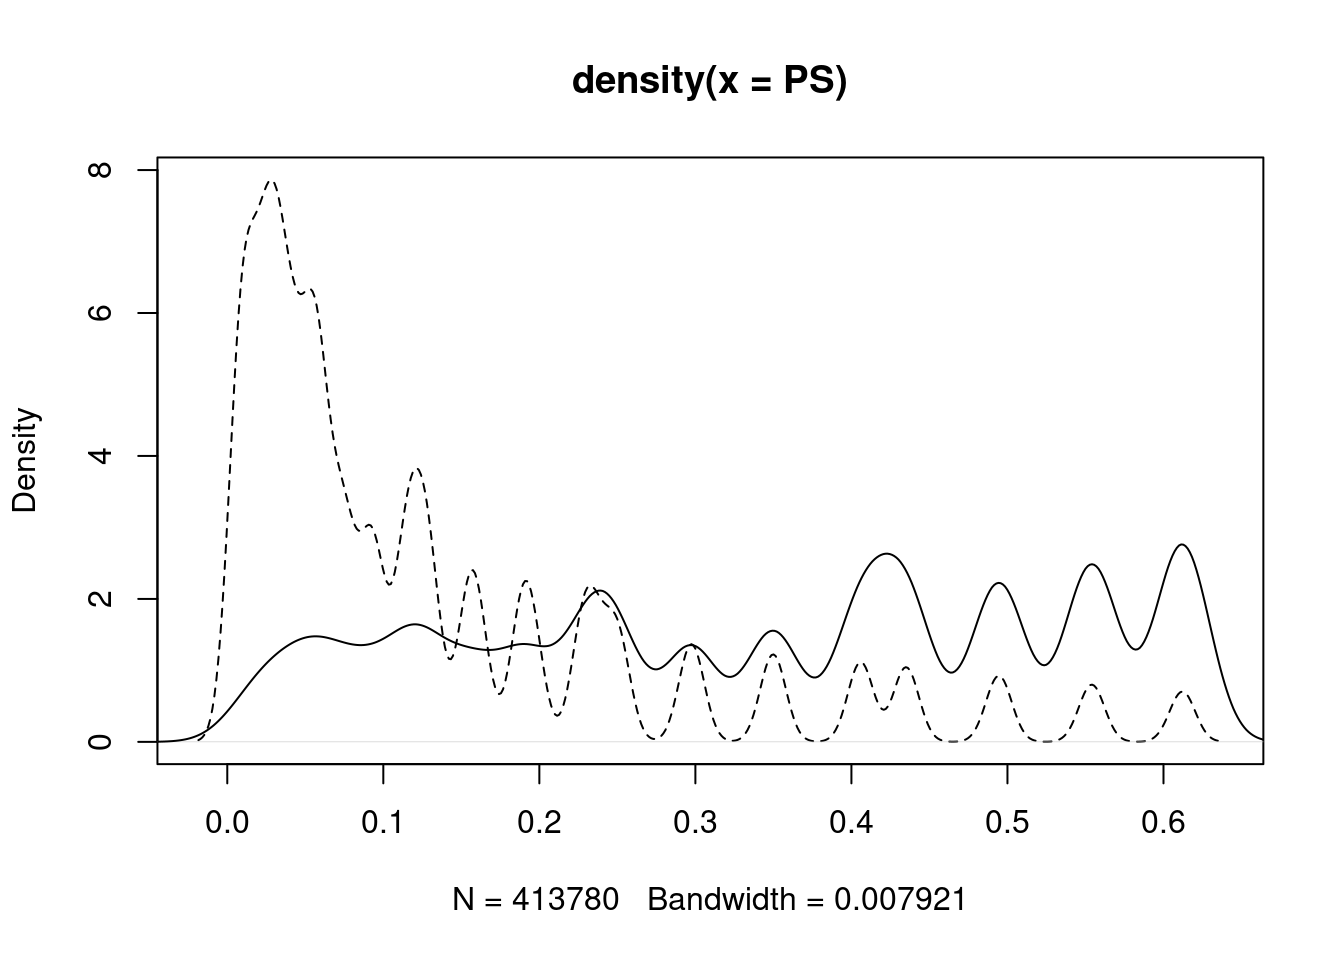
\includegraphics{causInf2-s_files/figure-latex/propScore-1.pdf}

How different are the distributions? Are they sufficiently overlapping?

\begin{enumerate}
\def\labelenumi{\arabic{enumi}.}
\setcounter{enumi}{2}
\tightlist
\item
  Compute the weights \(W_i = 1/\text{PS}_i\), when \(X_i=1\), and
  \(W_i = 1/(1-\text{PS}_i)\), when \(X_i=0\). Look at the sum as well as
  the distribution summary of the weights in the exposure groups. The
  sum of weights should be close to \(n\) in both groups.
\end{enumerate}

\begin{Shaded}
\begin{Highlighting}[]
\NormalTok{dd}\SpecialCharTok{$}\NormalTok{w }\OtherTok{\textless{}{-}} \FunctionTok{ifelse}\NormalTok{(dd}\SpecialCharTok{$}\NormalTok{x }\SpecialCharTok{==} \DecValTok{1}\NormalTok{, }\DecValTok{1} \SpecialCharTok{/}\NormalTok{ dd}\SpecialCharTok{$}\NormalTok{PS, }\DecValTok{1} \SpecialCharTok{/}\NormalTok{ (}\DecValTok{1} \SpecialCharTok{{-}}\NormalTok{ dd}\SpecialCharTok{$}\NormalTok{PS))}
\FunctionTok{with}\NormalTok{(dd, }\FunctionTok{tapply}\NormalTok{(w, x, sum))}
\end{Highlighting}
\end{Shaded}

\begin{verbatim}
##        0        1 
## 498880.5 565237.5
\end{verbatim}

\begin{enumerate}
\def\labelenumi{\arabic{enumi}.}
\setcounter{enumi}{3}
\tightlist
\item
  Compute now the weighted estimates of the counterfactual risks for
  both exposure categories \[ \widehat{E}_w(Y^{X = x}) =
  \frac{ \sum_{i=1}^n {\mathbf 1}_{ \{X_i=x\} } W_i Y_i }
     {\sum_{i=1}^n {\mathbf 1}_{ \{X_i=x\} }W_i} =
   \frac{ \sum_{X_i = x} W_i Y_i }{\sum_{X_i=x} W_i}, \quad x = 0,1, \]
  and their causal contrasts, for instance
  \[ \widehat{\text{RD}}_{w} = \widehat{E}_w(Y^{X = 1}) -
                \widehat{E}_w(Y^{X = 0})
   =   \frac{ \sum_{i=1}^n X_i W_i Y_i }{\sum_{i=1}^n X_i W_i} -
      \frac{ \sum_{i=1}^n (1-X_i) W_i Y_i }{\sum_{i=1}^n (1-X_i) W_i}
  \]
\end{enumerate}

\begin{Shaded}
\begin{Highlighting}[]
\NormalTok{EY1.w }\OtherTok{\textless{}{-}} \FunctionTok{sum}\NormalTok{(dd}\SpecialCharTok{$}\NormalTok{x }\SpecialCharTok{*}\NormalTok{ dd}\SpecialCharTok{$}\NormalTok{w }\SpecialCharTok{*}\NormalTok{ dd}\SpecialCharTok{$}\NormalTok{y) }\SpecialCharTok{/} \FunctionTok{sum}\NormalTok{(dd}\SpecialCharTok{$}\NormalTok{x }\SpecialCharTok{*}\NormalTok{ dd}\SpecialCharTok{$}\NormalTok{w)}
\NormalTok{EY0.w }\OtherTok{\textless{}{-}} \FunctionTok{sum}\NormalTok{((}\DecValTok{1} \SpecialCharTok{{-}}\NormalTok{ dd}\SpecialCharTok{$}\NormalTok{x) }\SpecialCharTok{*}\NormalTok{ dd}\SpecialCharTok{$}\NormalTok{w }\SpecialCharTok{*}\NormalTok{ dd}\SpecialCharTok{$}\NormalTok{y) }\SpecialCharTok{/} \FunctionTok{sum}\NormalTok{((}\DecValTok{1} \SpecialCharTok{{-}}\NormalTok{ dd}\SpecialCharTok{$}\NormalTok{x) }\SpecialCharTok{*}\NormalTok{ dd}\SpecialCharTok{$}\NormalTok{w)}
\FunctionTok{round}\NormalTok{(}\FunctionTok{Contr}\NormalTok{(EY1.w, EY0.w), }\DecValTok{4}\NormalTok{)}
\end{Highlighting}
\end{Shaded}

\begin{verbatim}
##                   RD     RR     OR 
## 0.8037 0.6519 0.1518 1.2329 2.1868
\end{verbatim}

These estimates seem to be somewhat downward biased when comparing to
true values. Could this be because of omitting the relatively strong
product term effect of \(Z_2\) and \(Z_4\)?

5.Let us attempt to correct the estimates by a double robust approach
called augmented IPW estimation (AIPW), which combines the g-formula and
the IPW approach. The AIPW-estimator can be expressed in two ways:
either an IPW-corrected g-formula estimator, or a g-corrected
IPW-estimator.

\[
\begin{aligned}
 \widehat{E}_a(Y^{X=x}) & = \widehat{E}_g(Y^{X=x}) +
   \frac{1}{n} \sum_{i=1}^n \frac{ {\mathbf 1}_{\{X_i=x\}} W_i ( Y_i - \widetilde{Y}_i^{X_i=x} ) }
   {\sum_{i=1}^n {\mathbf 1}_{\{X_i=x\}} W_i} \\
       & =   \widehat{E}_w(Y^{X=x}) -
    \frac{1}{n} \sum_{i=1}^n \left[ \frac{ {\mathbf 1}_{\{X_i=x\}} W_i }
            {\sum_{i=1}^n {\mathbf 1}_{\{X_i=x\}} W_i } - 1 \right] \widetilde{Y}_i^{X_i=x}.
\end{aligned}
\]

\begin{Shaded}
\begin{Highlighting}[]
\NormalTok{EY1.a }\OtherTok{\textless{}{-}}\NormalTok{ EY1.g }\SpecialCharTok{+} \FunctionTok{mean}\NormalTok{(dd}\SpecialCharTok{$}\NormalTok{x }\SpecialCharTok{*}\NormalTok{ (dd}\SpecialCharTok{$}\NormalTok{y }\SpecialCharTok{{-}}\NormalTok{ dd}\SpecialCharTok{$}\NormalTok{yp1) }\SpecialCharTok{*}\NormalTok{ dd}\SpecialCharTok{$}\NormalTok{w }\SpecialCharTok{/} \FunctionTok{sum}\NormalTok{(dd}\SpecialCharTok{$}\NormalTok{x }\SpecialCharTok{*}\NormalTok{ dd}\SpecialCharTok{$}\NormalTok{w))}
\DocumentationTok{\#\#  or   EY1.w {-} mean( ( ( dd$x*dd$w /sum(dd$x*dd$w) ) {-} 1 )*dd$yp1 )}
\NormalTok{EY0.a }\OtherTok{\textless{}{-}}\NormalTok{ EY0.g }\SpecialCharTok{+} \FunctionTok{mean}\NormalTok{((}\DecValTok{1} \SpecialCharTok{{-}}\NormalTok{ dd}\SpecialCharTok{$}\NormalTok{x) }\SpecialCharTok{*}\NormalTok{ (dd}\SpecialCharTok{$}\NormalTok{y }\SpecialCharTok{{-}}\NormalTok{ dd}\SpecialCharTok{$}\NormalTok{yp0) }\SpecialCharTok{*}\NormalTok{ dd}\SpecialCharTok{$}\NormalTok{w }\SpecialCharTok{/} \FunctionTok{sum}\NormalTok{((}\DecValTok{1} \SpecialCharTok{{-}}\NormalTok{ dd}\SpecialCharTok{$}\NormalTok{x) }\SpecialCharTok{*}\NormalTok{ dd}\SpecialCharTok{$}\NormalTok{w))}
\DocumentationTok{\#\#  or   EY0.w {-} mean( ( ( (1{-}dd$x)*dd$w/sum((1{-}dd$x)*dd$w) ) {-} 1 )*dd$yp0 )}
\FunctionTok{round}\NormalTok{(}\FunctionTok{Contr}\NormalTok{(EY1.a, EY0.a), }\DecValTok{4}\NormalTok{)}
\end{Highlighting}
\end{Shaded}

\begin{verbatim}
##                   RD     RR     OR 
## 0.8330 0.6508 0.1822 1.2800 2.6763
\end{verbatim}

Compare these results with those obtained by g-formula and by
non-augmented IPW method. Was augmentation successful?

\section{\texorpdfstring{Improving IPW estimation and using R package \texttt{PSweight}}{Improving IPW estimation and using R package PSweight}}\label{improving-ipw-estimation-and-using-r-package-psweight}

We now try to improve IPW-estimation by a richer exposure model. In
computations we shall utilize the R package \texttt{PSweight} (see \href{https://cran.r-project.org/web/packages/PSweight/vignettes/vignette.pdf}{PSweight
vignette}).

\begin{enumerate}
\def\labelenumi{\arabic{enumi}.}
\tightlist
\item
  First, we compute the weights from a more flexible exposure model
  which contains all pairwise product terms of the parents of \(X\).
  According to the causal diagram, \(Z_1\) is not in that subset, so it
  is left out. The exposure model is specified and the weights are
  obtained as follows.
\end{enumerate}

\begin{Shaded}
\begin{Highlighting}[]
\NormalTok{mX2 }\OtherTok{\textless{}{-}} \FunctionTok{glm}\NormalTok{(x }\SpecialCharTok{\textasciitilde{}}\NormalTok{ (z2 }\SpecialCharTok{+}\NormalTok{ z3 }\SpecialCharTok{+}\NormalTok{ z4)}\SpecialCharTok{\^{}}\DecValTok{2}\NormalTok{, }\AttributeTok{family =}\NormalTok{ binomial, }\AttributeTok{data =}\NormalTok{ dd)}
\FunctionTok{round}\NormalTok{(}\FunctionTok{ci.lin}\NormalTok{(mX2, }\AttributeTok{Exp =} \ConstantTok{TRUE}\NormalTok{)[, }\FunctionTok{c}\NormalTok{(}\DecValTok{1}\NormalTok{, }\DecValTok{5}\NormalTok{)], }\DecValTok{3}\NormalTok{)}
\end{Highlighting}
\end{Shaded}

\begin{verbatim}
##             Estimate exp(Est.)
## (Intercept)   -5.085     0.006
## z2             0.143     1.154
## z3             0.243     1.275
## z4             0.527     1.693
## z2:z3         -0.003     0.997
## z2:z4          0.376     1.456
## z3:z4          0.001     1.001
\end{verbatim}

\begin{Shaded}
\begin{Highlighting}[]
\NormalTok{psw }\OtherTok{\textless{}{-}} \FunctionTok{SumStat}\NormalTok{(}
  \AttributeTok{ps.formula =}\NormalTok{ mX2}\SpecialCharTok{$}\NormalTok{formula, }\AttributeTok{data =}\NormalTok{ dd,}
  \AttributeTok{weight =} \FunctionTok{c}\NormalTok{(}\StringTok{"IPW"}\NormalTok{, }\StringTok{"treated"}\NormalTok{, }\StringTok{"overlap"}\NormalTok{)}
\NormalTok{)}
\NormalTok{dd}\SpecialCharTok{$}\NormalTok{PS2 }\OtherTok{\textless{}{-}}\NormalTok{ psw}\SpecialCharTok{$}\NormalTok{propensity[, }\DecValTok{2}\NormalTok{] }\CommentTok{\# propensity scores extracted}
\FunctionTok{plot}\NormalTok{(}\FunctionTok{density}\NormalTok{(dd}\SpecialCharTok{$}\NormalTok{PS2[dd}\SpecialCharTok{$}\NormalTok{x }\SpecialCharTok{==} \DecValTok{0}\NormalTok{]), }\AttributeTok{lty =} \DecValTok{2}\NormalTok{)}
\FunctionTok{lines}\NormalTok{(}\FunctionTok{density}\NormalTok{(dd}\SpecialCharTok{$}\NormalTok{PS2[dd}\SpecialCharTok{$}\NormalTok{x }\SpecialCharTok{==} \DecValTok{1}\NormalTok{]), }\AttributeTok{lty =} \DecValTok{1}\NormalTok{)}
\end{Highlighting}
\end{Shaded}

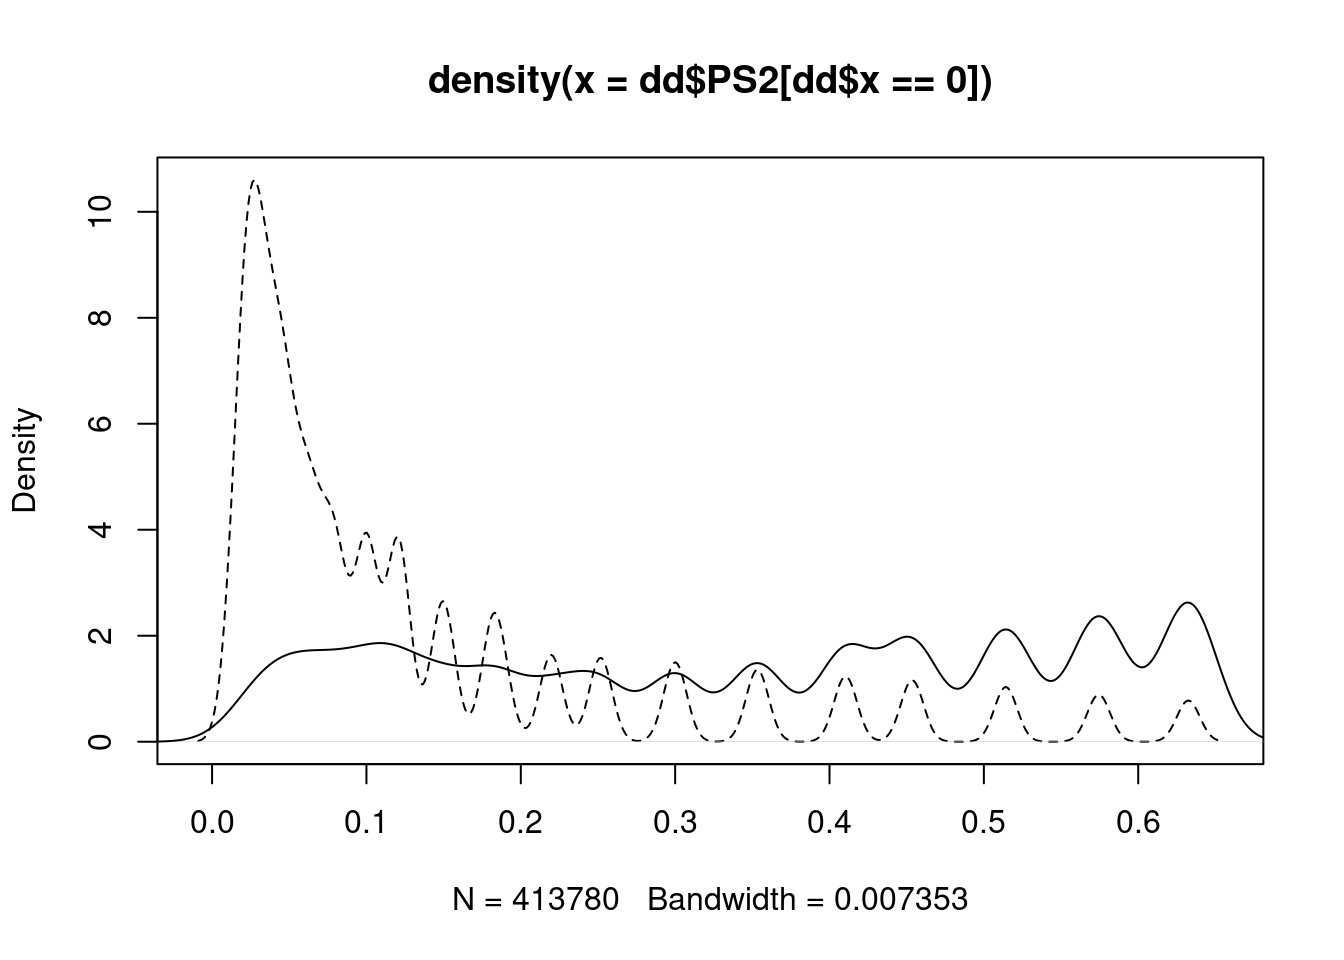
\includegraphics{causInf2-s_files/figure-latex/PSweight-1.pdf}

Note that apart from ordinary IPW, other types of weights can also also
obtained. These are relevant when estimating other kinds of causal
contrasts, like \emph{average treatment effect among the treated} (ATT) and
``average treatment effect in the overlap (or equipoise) population'\,'
(ATO).

\begin{enumerate}
\def\labelenumi{\arabic{enumi}.}
\setcounter{enumi}{1}
\tightlist
\item
  \texttt{PSweight} includes some useful tools to examine the properties of
  the distribution and to check the balance of the propensity scores,
  for instance
\end{enumerate}

\begin{Shaded}
\begin{Highlighting}[]
\FunctionTok{plot}\NormalTok{(psw, }\AttributeTok{type =} \StringTok{"balance"}\NormalTok{, }\AttributeTok{metric =} \StringTok{"PSD"}\NormalTok{)}
\end{Highlighting}
\end{Shaded}

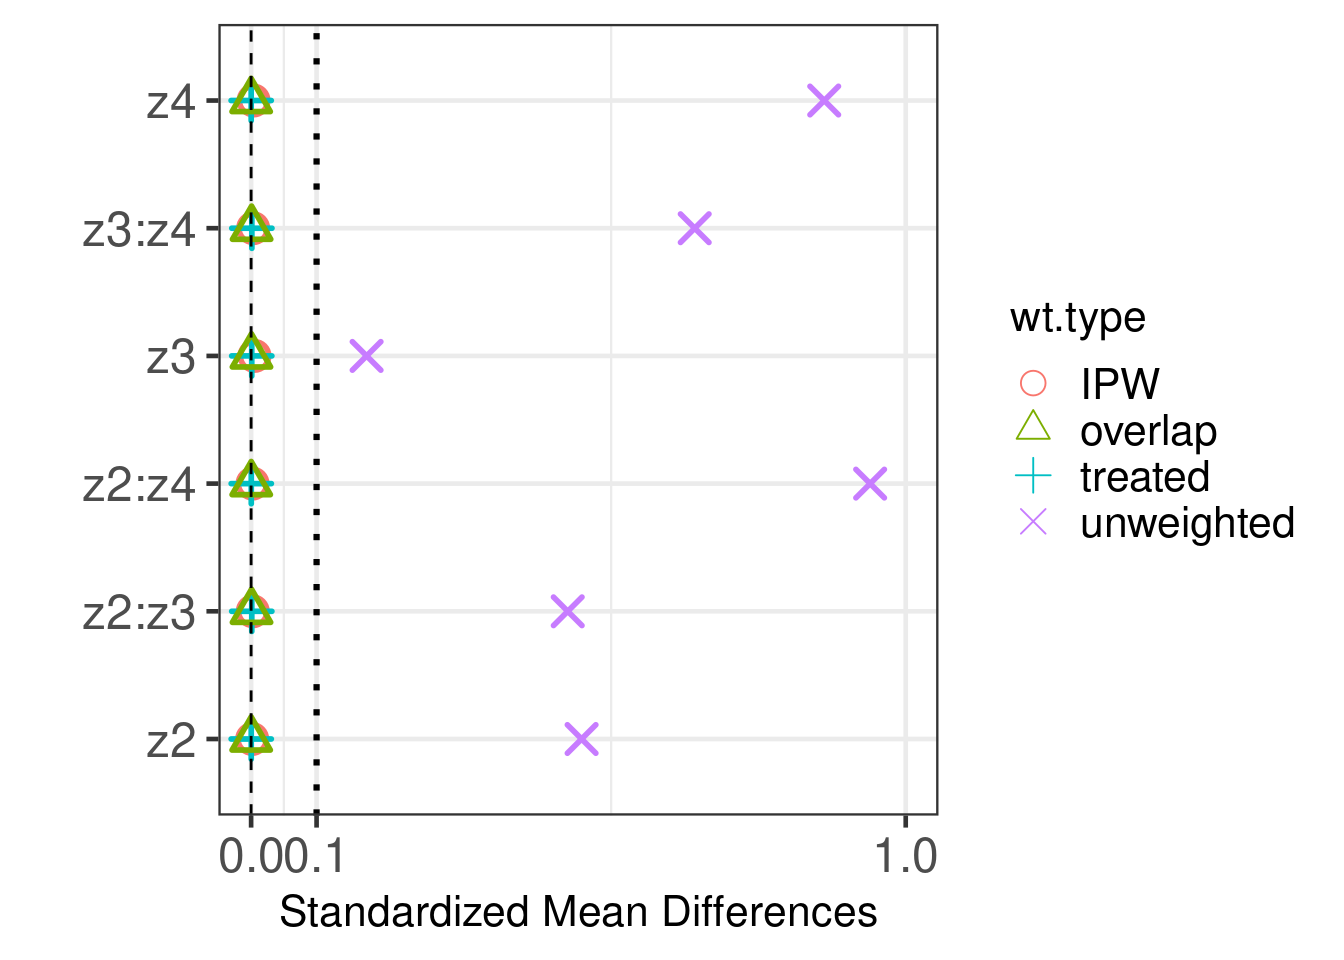
\includegraphics{causInf2-s_files/figure-latex/check balance-1.pdf}

It is desirable that the horisontal values of these measures for given
weights are less than 0.1.

\begin{enumerate}
\def\labelenumi{\arabic{enumi}.}
\setcounter{enumi}{2}
\tightlist
\item
  Estimation and reporting of the causal contrasts. For relative
  contrasts, the summary method provides the results on the log-scale.
\end{enumerate}

\begin{Shaded}
\begin{Highlighting}[]
\NormalTok{ipwest }\OtherTok{\textless{}{-}} \FunctionTok{PSweight}\NormalTok{(}\AttributeTok{ps.formula =}\NormalTok{ mX2, }\AttributeTok{yname =} \StringTok{"y"}\NormalTok{, }\AttributeTok{data =}\NormalTok{ dd, }\AttributeTok{weight =} \StringTok{"IPW"}\NormalTok{)}
\NormalTok{ipwest}
\end{Highlighting}
\end{Shaded}

\begin{verbatim}
## Original group value:  0, 1 
## 
## Point estimate: 
## 0.6526, 0.8255
\end{verbatim}

\begin{Shaded}
\begin{Highlighting}[]
\FunctionTok{summary}\NormalTok{(ipwest)}
\end{Highlighting}
\end{Shaded}

\begin{verbatim}
## 
## Closed-form inference: 
## 
## Original group value:  0, 1 
## 
## Contrast: 
##             0 1
## Contrast 1 -1 1
## 
##             Estimate Std.Error       lwr     upr  Pr(>|z|)    
## Contrast 1 0.1729179 0.0025636 0.1678934 0.17794 < 2.2e-16 ***
## ---
## Signif. codes:  0 '***' 0.001 '**' 0.01 '*' 0.05 '.' 0.1 ' ' 1
\end{verbatim}

\begin{Shaded}
\begin{Highlighting}[]
\NormalTok{(logRR.ipw }\OtherTok{\textless{}{-}} \FunctionTok{summary}\NormalTok{(ipwest, }\AttributeTok{type =} \StringTok{"RR"}\NormalTok{))}
\end{Highlighting}
\end{Shaded}

\begin{verbatim}
## 
## Closed-form inference: 
## 
## Inference in log scale: 
## Original group value:  0, 1 
## 
## Contrast: 
##             0 1
## Contrast 1 -1 1
## 
##             Estimate Std.Error       lwr     upr  Pr(>|z|)    
## Contrast 1 0.2350512 0.0031789 0.2288207 0.24128 < 2.2e-16 ***
## ---
## Signif. codes:  0 '***' 0.001 '**' 0.01 '*' 0.05 '.' 0.1 ' ' 1
\end{verbatim}

\begin{Shaded}
\begin{Highlighting}[]
\FunctionTok{round}\NormalTok{(}\FunctionTok{exp}\NormalTok{(logRR.ipw}\SpecialCharTok{$}\NormalTok{estimates[}\FunctionTok{c}\NormalTok{(}\DecValTok{1}\NormalTok{, }\DecValTok{4}\NormalTok{, }\DecValTok{5}\NormalTok{)]), }\DecValTok{3}\NormalTok{)}
\end{Highlighting}
\end{Shaded}

\begin{verbatim}
## [1] 1.265 1.257 1.273
\end{verbatim}

\begin{Shaded}
\begin{Highlighting}[]
\FunctionTok{round}\NormalTok{(}\FunctionTok{exp}\NormalTok{(}\FunctionTok{summary}\NormalTok{(ipwest, }\AttributeTok{type =} \StringTok{"OR"}\NormalTok{)}\SpecialCharTok{$}\NormalTok{estimates[}\FunctionTok{c}\NormalTok{(}\DecValTok{1}\NormalTok{, }\DecValTok{4}\NormalTok{, }\DecValTok{5}\NormalTok{)]), }\DecValTok{3}\NormalTok{)}
\end{Highlighting}
\end{Shaded}

\begin{verbatim}
## [1] 2.519 2.434 2.606
\end{verbatim}

Compare these with the previous IPW estimate and the AIPW estimate as
well as the true values. Have we obtained nearly unbiased results?

The standard errors provided by \texttt{PSweight} are by default based on the
empirical sandwich covariance matrix and application of delta method as
appropriate. Bootstrapping is also possible but is computationally very
intensive and is recommended to be used only in relatively small
samples.

\begin{enumerate}
\def\labelenumi{\arabic{enumi}.}
\setcounter{enumi}{3}
\tightlist
\item
  If we are interested in the effect of exposure among the exposed
  (like ATT) then the weights are \(W_i = 1\) for the exposed and
  \(W_i = \text{PS}_i/(1-\text{PS}_i)\) for the unexposed. Call again
  \texttt{PSweight} but with another choice of weight:
\end{enumerate}

\begin{Shaded}
\begin{Highlighting}[]
\NormalTok{psatt }\OtherTok{\textless{}{-}} \FunctionTok{PSweight}\NormalTok{(}\AttributeTok{ps.formula =}\NormalTok{ mX2, }\AttributeTok{yname =} \StringTok{"y"}\NormalTok{, }\AttributeTok{data =}\NormalTok{ dd, }\AttributeTok{weight =} \StringTok{"treated"}\NormalTok{)}
\NormalTok{psatt}
\end{Highlighting}
\end{Shaded}

\begin{verbatim}
## Original group value:  0, 1 
## Treatment group value:  1 
## 
## Point estimate: 
## 0.7667, 0.8949
\end{verbatim}

\begin{Shaded}
\begin{Highlighting}[]
\FunctionTok{round}\NormalTok{(}\FunctionTok{summary}\NormalTok{(psatt)}\SpecialCharTok{$}\NormalTok{estimates[}\DecValTok{1}\NormalTok{], }\DecValTok{4}\NormalTok{)}
\end{Highlighting}
\end{Shaded}

\begin{verbatim}
## [1] 0.1282
\end{verbatim}

\begin{Shaded}
\begin{Highlighting}[]
\FunctionTok{round}\NormalTok{(}\FunctionTok{exp}\NormalTok{(}\FunctionTok{summary}\NormalTok{(psatt, }\AttributeTok{type =} \StringTok{"RR"}\NormalTok{)}\SpecialCharTok{$}\NormalTok{estimates[}\DecValTok{1}\NormalTok{]), }\DecValTok{3}\NormalTok{)}
\end{Highlighting}
\end{Shaded}

\begin{verbatim}
## [1] 1.167
\end{verbatim}

\begin{Shaded}
\begin{Highlighting}[]
\FunctionTok{round}\NormalTok{(}\FunctionTok{exp}\NormalTok{(}\FunctionTok{summary}\NormalTok{(psatt, }\AttributeTok{type =} \StringTok{"OR"}\NormalTok{)}\SpecialCharTok{$}\NormalTok{estimates[}\DecValTok{1}\NormalTok{]), }\DecValTok{3}\NormalTok{)}
\end{Highlighting}
\end{Shaded}

\begin{verbatim}
## [1] 2.592
\end{verbatim}

Compare the results here with those obtained by g-formula in item 4(e)
and with the true contrasts in item 4(f) above.

\section{Targeted maximum likelihood estimation (TMLE)}\label{targeted-maximum-likelihood-estimation-tmle}

We now consider now another double robust approach, known as targeted
maximum likelihood estimation (TMLE). It also corrects the estimator
obtained from the outcome model by elements that are derived from the
exposure model. See \href{https://doi.org/10.1093/aje/kww165}{Schuler and Rose
(2017)} for more details

\begin{enumerate}
\def\labelenumi{\arabic{enumi}.}
\tightlist
\item
  The first step is to utilize the propensity scores obtained above
  and define the so called clever covariates
\end{enumerate}

\begin{Shaded}
\begin{Highlighting}[]
\NormalTok{dd}\SpecialCharTok{$}\NormalTok{H1 }\OtherTok{\textless{}{-}}\NormalTok{ dd}\SpecialCharTok{$}\NormalTok{x }\SpecialCharTok{/}\NormalTok{ dd}\SpecialCharTok{$}\NormalTok{PS2}
\NormalTok{dd}\SpecialCharTok{$}\NormalTok{H0 }\OtherTok{\textless{}{-}}\NormalTok{ (}\DecValTok{1} \SpecialCharTok{{-}}\NormalTok{ dd}\SpecialCharTok{$}\NormalTok{x) }\SpecialCharTok{/}\NormalTok{ (}\DecValTok{1} \SpecialCharTok{{-}}\NormalTok{ dd}\SpecialCharTok{$}\NormalTok{PS2)}
\end{Highlighting}
\end{Shaded}

\begin{enumerate}
\def\labelenumi{\arabic{enumi}.}
\setcounter{enumi}{1}
\tightlist
\item
  Then, a working model is fitted for the outcome, in which the clever
  covariates are explanatory variables, but the model also includes
  the previously fitted linear predictor
  \(\widehat{\eta}_i = \text{logit}(\widehat Y_i)\) from the original
  outcome model \texttt{mY} as an offset term. Moreover, the intercept is
  removed.
\end{enumerate}

\begin{Shaded}
\begin{Highlighting}[]
\NormalTok{epsmod }\OtherTok{\textless{}{-}} \FunctionTok{glm}\NormalTok{(y }\SpecialCharTok{\textasciitilde{}} \SpecialCharTok{{-}}\DecValTok{1} \SpecialCharTok{+}\NormalTok{ H0 }\SpecialCharTok{+}\NormalTok{ H1 }\SpecialCharTok{+} \FunctionTok{offset}\NormalTok{(}\FunctionTok{qlogis}\NormalTok{(yh)),}
  \AttributeTok{family =} \FunctionTok{binomial}\NormalTok{(}\AttributeTok{link =}\NormalTok{ logit), }\AttributeTok{data =}\NormalTok{ dd}
\NormalTok{)}
\NormalTok{eps }\OtherTok{\textless{}{-}} \FunctionTok{coef}\NormalTok{(epsmod)}
\NormalTok{eps}
\end{Highlighting}
\end{Shaded}

\begin{verbatim}
##           H0           H1 
##  0.007197951 -0.002859654
\end{verbatim}

\begin{enumerate}
\def\labelenumi{\arabic{enumi}.}
\setcounter{enumi}{2}
\tightlist
\item
  The logit-transformed predicted values \(\widetilde{Y}_i^{X_i=1}\) and
  \(\widetilde{Y}_i^{X_i=0}\) of counterfactual individual risks from
  the original outcome model are now corrected by the estimated
  coefficients of the clever covariates, and the corrected predictions
  are returned to the original scale.
\end{enumerate}

\begin{Shaded}
\begin{Highlighting}[]
\NormalTok{yp0.H }\OtherTok{\textless{}{-}} \FunctionTok{plogis}\NormalTok{(}\FunctionTok{qlogis}\NormalTok{(dd}\SpecialCharTok{$}\NormalTok{yp0) }\SpecialCharTok{+}\NormalTok{ eps[}\DecValTok{1}\NormalTok{] }\SpecialCharTok{/}\NormalTok{ (}\DecValTok{1} \SpecialCharTok{{-}}\NormalTok{ dd}\SpecialCharTok{$}\NormalTok{PS2))}
\NormalTok{yp1.H }\OtherTok{\textless{}{-}} \FunctionTok{plogis}\NormalTok{(}\FunctionTok{qlogis}\NormalTok{(dd}\SpecialCharTok{$}\NormalTok{yp1) }\SpecialCharTok{+}\NormalTok{ eps[}\DecValTok{2}\NormalTok{] }\SpecialCharTok{/}\NormalTok{ dd}\SpecialCharTok{$}\NormalTok{PS2)}
\end{Highlighting}
\end{Shaded}

\begin{itemize}
\tightlist
\item
\end{itemize}

Estimates of the causal contrasts:

\begin{Shaded}
\begin{Highlighting}[]
\NormalTok{EY0.t }\OtherTok{\textless{}{-}} \FunctionTok{mean}\NormalTok{(yp0.H)}
\NormalTok{EY1.t }\OtherTok{\textless{}{-}} \FunctionTok{mean}\NormalTok{(yp1.H)}
\FunctionTok{round}\NormalTok{(}\FunctionTok{Contr}\NormalTok{(EY1.t, EY0.t), }\DecValTok{4}\NormalTok{)}
\end{Highlighting}
\end{Shaded}

\begin{verbatim}
##                   RD     RR     OR 
## 0.8246 0.6526 0.1720 1.2635 2.5020
\end{verbatim}

Compare these with previous results and with the true values.

\section{TMLE with SuperLearner}\label{tmle-with-superlearner}

Let us finally apply some fashionable tools of statistical learning, aka
\emph{machine learning}, using the package \texttt{SuperLearner} to fit flexible
models for both exposure and outcome. As this method is computationally
much more demanding, we illustrate its use by a sample of 2000 subjects
only.

\begin{enumerate}
\def\labelenumi{\arabic{enumi}.}
\tightlist
\item
  A simple random sample of \(n=2000\) is drawn from the population.
\end{enumerate}

\begin{Shaded}
\begin{Highlighting}[]
\FunctionTok{set.seed}\NormalTok{(}\DecValTok{7622}\NormalTok{)}
\NormalTok{n }\OtherTok{\textless{}{-}} \DecValTok{2000}
\NormalTok{sampind }\OtherTok{\textless{}{-}} \FunctionTok{sample}\NormalTok{(N, n)}
\NormalTok{samp }\OtherTok{\textless{}{-}}\NormalTok{ dd[sampind, ]}
\end{Highlighting}
\end{Shaded}

\begin{enumerate}
\def\labelenumi{\arabic{enumi}.}
\setcounter{enumi}{1}
\tightlist
\item
  The algorithms to be used in this exercise are chosen
\end{enumerate}

\begin{Shaded}
\begin{Highlighting}[]
\NormalTok{SL.library }\OtherTok{\textless{}{-}} \FunctionTok{c}\NormalTok{(}
  \StringTok{"SL.glm"}\NormalTok{, }\StringTok{"SL.step"}\NormalTok{, }\StringTok{"SL.step.interaction"}\NormalTok{,}
  \StringTok{"SL.glm.interaction"}\NormalTok{, }\StringTok{"SL.gam"}\NormalTok{,}
  \StringTok{"SL.randomForest"}\NormalTok{, }\StringTok{"SL.rpart"}
\NormalTok{)}
\end{Highlighting}
\end{Shaded}

\begin{enumerate}
\def\labelenumi{\arabic{enumi}.}
\setcounter{enumi}{2}
\tightlist
\item
  Function \texttt{tmle()} computes estimates of the causal contrasts of
  interest. Argument \texttt{A} is for the exposure variable, and argument
  \texttt{W} contains the confounders.
\end{enumerate}

The run can take a while \ldots{}

\begin{Shaded}
\begin{Highlighting}[]
\NormalTok{tmlest }\OtherTok{\textless{}{-}} \FunctionTok{tmle}\NormalTok{(}
  \AttributeTok{Y =}\NormalTok{ samp}\SpecialCharTok{$}\NormalTok{y, }\AttributeTok{A =}\NormalTok{ samp}\SpecialCharTok{$}\NormalTok{x, }\AttributeTok{W =}\NormalTok{ samp[, }\FunctionTok{c}\NormalTok{(}\StringTok{"z1"}\NormalTok{, }\StringTok{"z2"}\NormalTok{, }\StringTok{"z3"}\NormalTok{, }\StringTok{"z4"}\NormalTok{)],}
  \AttributeTok{family =} \StringTok{"binomial"}\NormalTok{, }\AttributeTok{Q.SL.library =}\NormalTok{ SL.library,}
  \AttributeTok{g.SL.library =}\NormalTok{ SL.library}
\NormalTok{)}
\FunctionTok{summary}\NormalTok{(tmlest)}
\end{Highlighting}
\end{Shaded}

Let us take a closer look at the results. In the beginning are reported
the fractions by which the separate algorithms contribute to the
combined algorithm. After that are given estimates of the causal
contrasts together with their estimated variances and 95\% confidence
intervals. The variance of each contrast (on log-scale for RR and OR) is
estimated as the variance of the empirical influence curve divided by
\(n\), the number of i.i.d. units of observation. Furthermore, causal risk
differences are estimated also for those factually exposed and
unexposed, respectively.

Note that because this analysis was based on sample data, the estimates
are most probably deviating from the true values because of pure random
error. Therefore it is not possible to assess the magnitude of a
possible bias from a single sample.

\textbf{Homework.} When you have more time, try to run \texttt{tmle} on as large
sample as is possible and compare its results with previous ones
computed for the whole target population.

\chapter{Time-dependent variables and multiple states}\label{time-dependent-variables-and-multiple-states}

The following practical exercise is based on the data from paper:

\begin{quote}
P Hovind, L Tarnow, P Rossing, B Carstensen, and HH Parving:
Improved survival in patients obtaining remission of nephrotic range
albuminuria in diabetic nephropathy.
\emph{Kidney Int}, \textbf{66}(3):1180--1186, Sept 2004.
\end{quote}

You can find a \texttt{.pdf}-version of the paper here:
\url{http://BendixCarstensen.com/AdvCoh/papers/Hovind.2004.pdf}

\section{The renal failure dataset}\label{the-renal-failure-dataset}

The dataset \texttt{renal.dta} contains data on follow up of 125
patients from Steno Diabetes Center. They enter the study when they
are diagnosed with nephrotic range albuminuria (NRA). This is a
condition where the levels of albumin in the urine is exceeds a
certain level as a sign of kidney disease. The levels may however drop
as a consequence of treatment, this is called remission. Patients exit
the study at death or kidney failure (dialysis or transplant).

\begin{longtable}[]{@{}ll@{}}
\toprule\noalign{}
Variable & Description \\
\midrule\noalign{}
\endhead
\bottomrule\noalign{}
\endlastfoot
\texttt{id} & Patient id \\
\texttt{sex} & 1=male, 2=female \\
\texttt{dob} & Date of birth \\
\texttt{doe} & Date of entry into the study (2.5 years after NRA) \\
\texttt{dor} & Date of remission. Missing if no remission has occurred \\
\texttt{dox} & Date of exit from study \\
\texttt{event} & Exit status: 1,2,3=event (death, ESRD), 0=censored \\
\end{longtable}

\begin{enumerate}
\def\labelenumi{\arabic{enumi}.}
\item
  The dataset is in Stata-format, so you must read the dataset
  using \texttt{read.dta} from the \texttt{foreign} package (which is
  part of the standard \texttt{R}-distribution). At the same time, convert
  \texttt{sex} to a proper factor. Choose where to read the dataset.

\begin{Shaded}
\begin{Highlighting}[]
\FunctionTok{library}\NormalTok{(Epi)}
\FunctionTok{library}\NormalTok{(survival)}
\FunctionTok{library}\NormalTok{(mgcv)}
\end{Highlighting}
\end{Shaded}

\begin{verbatim}
Loading required package: nlme
\end{verbatim}

\begin{verbatim}
This is mgcv 1.9-1. For overview type 'help("mgcv-package")'.
\end{verbatim}

\begin{Shaded}
\begin{Highlighting}[]
\FunctionTok{library}\NormalTok{(foreign)}
\CommentTok{\# renal \textless{}{-} read.dta(}
\CommentTok{\#  "https://raw.githubusercontent.com/SPE{-}R/SPE/master/pracs/data/renal.dta")}
\NormalTok{renal }\OtherTok{\textless{}{-}} \FunctionTok{read.dta}\NormalTok{(}\StringTok{"http://BendixCarstensen.com/SPE/data/renal.dta"}\NormalTok{)}
\NormalTok{renal}\SpecialCharTok{$}\NormalTok{sex }\OtherTok{\textless{}{-}} \FunctionTok{factor}\NormalTok{(renal}\SpecialCharTok{$}\NormalTok{sex, }\AttributeTok{labels =} \FunctionTok{c}\NormalTok{(}\StringTok{"M"}\NormalTok{, }\StringTok{"F"}\NormalTok{))}
\FunctionTok{head}\NormalTok{(renal)}
\end{Highlighting}
\end{Shaded}
\item
  Use the \texttt{Lexis} function to declare the data as
  survival data with age, calendar time and time since entry into
  the study as timescales. Label any event \(>0\) as \emph{ESRD},
  i.e.~renal death (death of kidney (transplant or dialysis), or
  person).
  Note that you must make sure that the \emph{alive} state (here
  \texttt{NRA}) is the first, as \texttt{Lexis} assumes that
  everyone starts in this state (unless of course
  \texttt{entry.status} is specified):

\begin{Shaded}
\begin{Highlighting}[]
\NormalTok{Lr }\OtherTok{\textless{}{-}} \FunctionTok{Lexis}\NormalTok{(}\AttributeTok{entry =} \FunctionTok{list}\NormalTok{(}\AttributeTok{per =}\NormalTok{ doe,}
                         \AttributeTok{age =}\NormalTok{ doe }\SpecialCharTok{{-}}\NormalTok{ dob,}
                         \AttributeTok{tfi =} \DecValTok{0}\NormalTok{),}
             \AttributeTok{exit =} \FunctionTok{list}\NormalTok{(}\AttributeTok{per =}\NormalTok{ dox),}
      \AttributeTok{exit.status =} \FunctionTok{factor}\NormalTok{(event }\SpecialCharTok{\textgreater{}} \DecValTok{0}\NormalTok{, }\AttributeTok{labels =} \FunctionTok{c}\NormalTok{(}\StringTok{"NRA"}\NormalTok{, }\StringTok{"ESRD"}\NormalTok{)),}
             \AttributeTok{data =}\NormalTok{ renal)}
\end{Highlighting}
\end{Shaded}

\begin{verbatim}
NOTE: entry.status has been set to "NRA" for all.
\end{verbatim}

\begin{Shaded}
\begin{Highlighting}[]
\FunctionTok{str}\NormalTok{(Lr)}
\end{Highlighting}
\end{Shaded}

\begin{verbatim}
Classes 'Lexis' and 'data.frame':   125 obs. of  14 variables:
 $ per    : num  1996 1990 1988 1995 1988 ...
 $ age    : num  28.1 30.2 25.8 44.5 26.6 ...
 $ tfi    : num  0 0 0 0 0 0 0 0 0 0 ...
 $ lex.dur: num  1.08 6.6 5.39 8.75 16.07 ...
 $ lex.Cst: Factor w/ 2 levels "NRA","ESRD": 1 1 1 1 1 1 1 1 1 1 ...
 $ lex.Xst: Factor w/ 2 levels "NRA","ESRD": 2 2 2 1 1 2 2 1 2 1 ...
 $ lex.id : int  1 2 3 4 5 6 7 8 9 10 ...
 $ id     : num  17 26 27 33 42 46 47 55 62 64 ...
 $ sex    : Factor w/ 2 levels "M","F": 1 2 2 1 2 2 1 1 2 1 ...
 $ dob    : num  1968 1959 1962 1951 1961 ...
 $ doe    : num  1996 1990 1988 1995 1988 ...
 $ dor    : num  NA 1990 NA 1996 1997 ...
 $ dox    : num  1997 1996 1993 2004 2004 ...
 $ event  : num  2 1 3 0 0 2 1 0 2 0 ...
 - attr(*, "time.scales")= chr [1:3] "per" "age" "tfi"
 - attr(*, "time.since")= chr [1:3] "" "" ""
 - attr(*, "breaks")=List of 3
  ..$ per: NULL
  ..$ age: NULL
  ..$ tfi: NULL
\end{verbatim}

\begin{Shaded}
\begin{Highlighting}[]
\FunctionTok{summary}\NormalTok{(Lr)}
\end{Highlighting}
\end{Shaded}

\begin{verbatim}

Transitions:
     To
From  NRA ESRD  Records:  Events: Risk time:  Persons:
  NRA  48   77       125       77    1084.67       125
\end{verbatim}

  Make sure you know what the variables in \texttt{Lr} stand for.
\item
  Visualize the follow-up in a Lexis-diagram, by using the
  \texttt{plot} method for \texttt{Lexis} objects.

\begin{Shaded}
\begin{Highlighting}[]
\FunctionTok{plot}\NormalTok{(Lr, }\AttributeTok{col =} \StringTok{"black"}\NormalTok{, }\AttributeTok{lwd =} \DecValTok{3}\NormalTok{)}
\end{Highlighting}
\end{Shaded}

  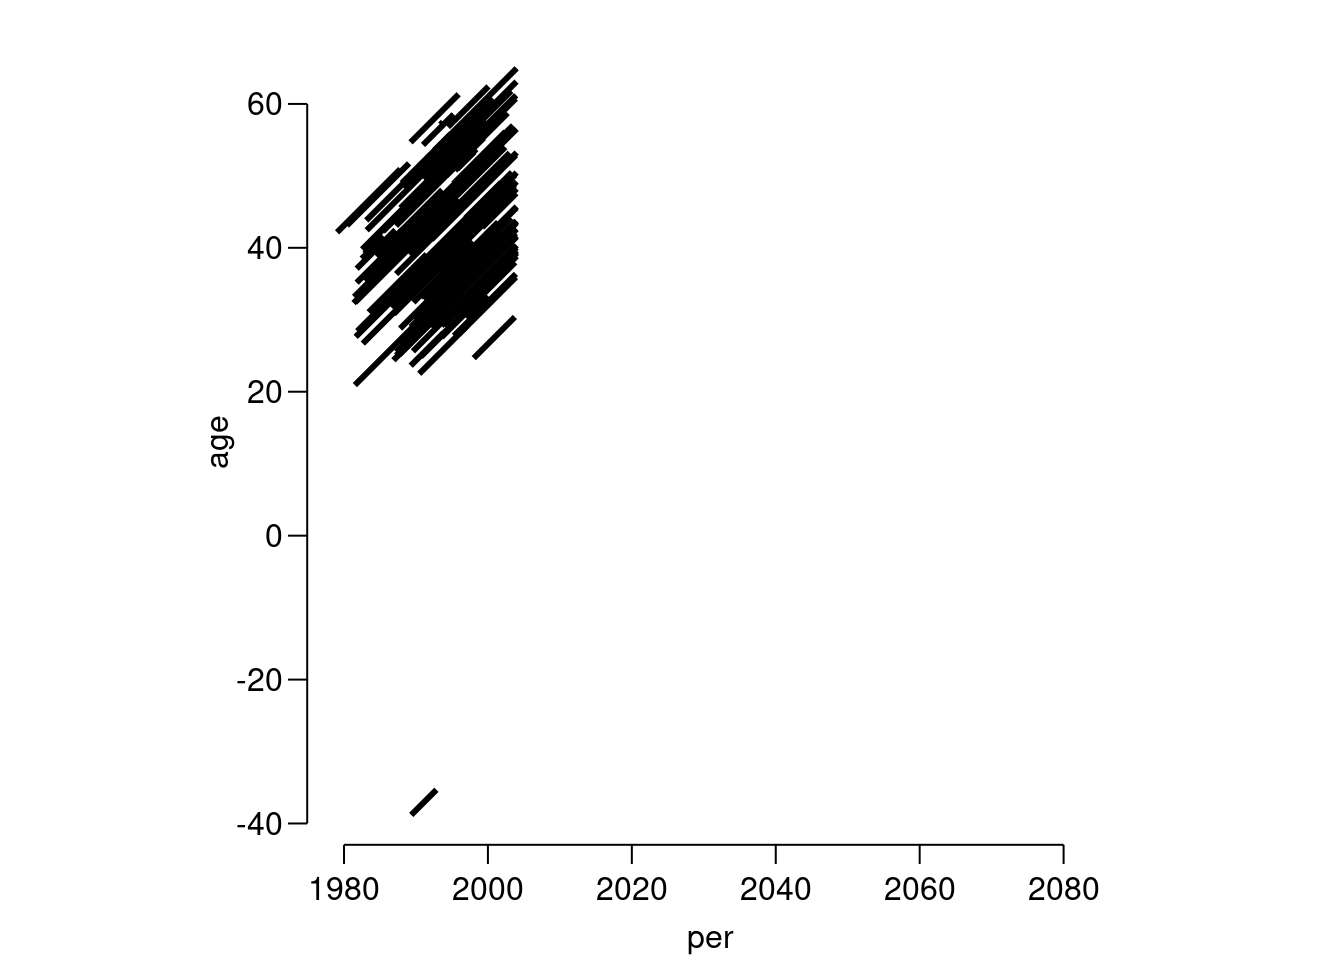
\includegraphics{renal-s_files/figure-latex/Lexis-ups-1.pdf}

\begin{Shaded}
\begin{Highlighting}[]
\FunctionTok{subset}\NormalTok{(Lr, age }\SpecialCharTok{\textless{}} \DecValTok{0}\NormalTok{)}
\end{Highlighting}
\end{Shaded}

\begin{verbatim}
 lex.id     per    age tfi lex.dur lex.Cst lex.Xst  id sex      dob      doe dor      dox
     88 1989.34 -38.81   0     3.5     NRA    ESRD 586   M 2028.155 1989.343  NA 1992.839
 event
     1
\end{verbatim}

  What is wrong here? List the data for the person with negative entry age.
\item
  Correct the data and make a new plot, for example by:

\begin{Shaded}
\begin{Highlighting}[]
\NormalTok{Lr }\OtherTok{\textless{}{-}} \FunctionTok{transform}\NormalTok{(Lr, }\AttributeTok{age =} \FunctionTok{ifelse}\NormalTok{(dob }\SpecialCharTok{\textgreater{}} \DecValTok{2000}\NormalTok{, age }\SpecialCharTok{+} \DecValTok{100}\NormalTok{, age),}
                    \AttributeTok{dob =} \FunctionTok{ifelse}\NormalTok{(dob }\SpecialCharTok{\textgreater{}} \DecValTok{2000}\NormalTok{, dob }\SpecialCharTok{{-}} \DecValTok{100}\NormalTok{, dob))}
\FunctionTok{subset}\NormalTok{(Lr, id }\SpecialCharTok{==} \DecValTok{586}\NormalTok{)}
\end{Highlighting}
\end{Shaded}

\begin{verbatim}
 lex.id     per   age tfi lex.dur lex.Cst lex.Xst  id sex      dob      doe dor      dox
     88 1989.34 61.19   0     3.5     NRA    ESRD 586   M 1928.155 1989.343  NA 1992.839
 event
     1
\end{verbatim}

\begin{Shaded}
\begin{Highlighting}[]
\FunctionTok{plot}\NormalTok{(Lr, }\AttributeTok{col =} \StringTok{"black"}\NormalTok{, }\AttributeTok{lwd =} \DecValTok{3}\NormalTok{)}
\end{Highlighting}
\end{Shaded}

  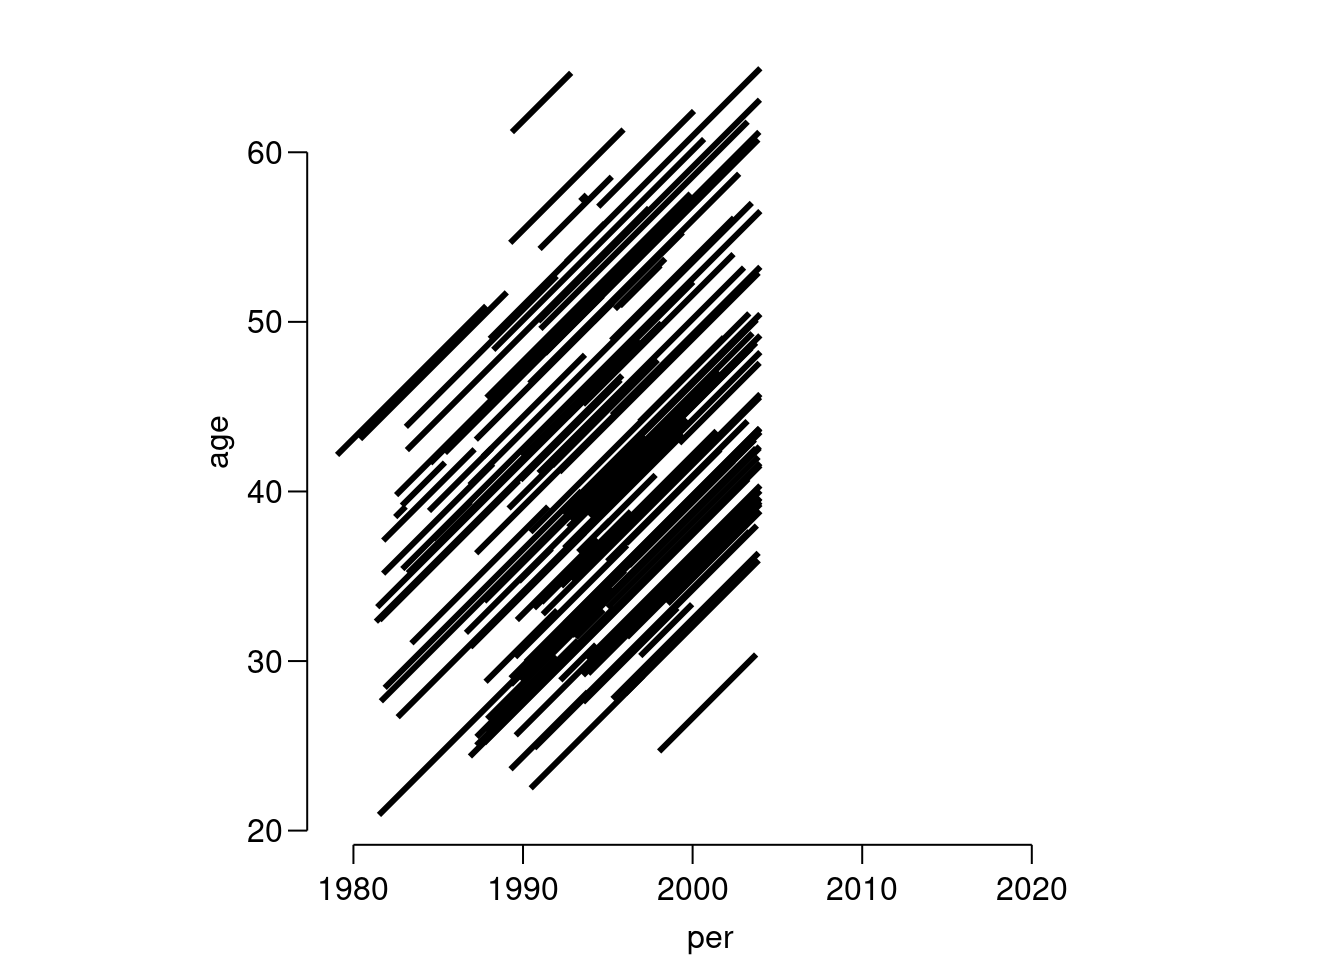
\includegraphics{renal-s_files/figure-latex/Lexis-def-1.pdf}
\item
  Now make a Cox-regression analysis of ESRD occurrence with
  the variables sex and age at entry into the study, using time
  since entry to the study as time scale.

\begin{Shaded}
\begin{Highlighting}[]
\NormalTok{mc }\OtherTok{\textless{}{-}} \FunctionTok{coxph}\NormalTok{(}\FunctionTok{Surv}\NormalTok{(lex.dur, lex.Xst }\SpecialCharTok{==} \StringTok{"ESRD"}\NormalTok{) }
            \SpecialCharTok{\textasciitilde{}} \FunctionTok{I}\NormalTok{(age }\SpecialCharTok{/} \DecValTok{10}\NormalTok{) }\SpecialCharTok{+}\NormalTok{ sex, }\AttributeTok{data =}\NormalTok{ Lr)}
\FunctionTok{summary}\NormalTok{(mc)}
\end{Highlighting}
\end{Shaded}

\begin{verbatim}
Call:
coxph(formula = Surv(lex.dur, lex.Xst == "ESRD") ~ I(age/10) + 
    sex, data = Lr)

  n= 125, number of events= 77 

             coef exp(coef) se(coef)      z Pr(>|z|)
I(age/10)  0.5514    1.7357   0.1402  3.932 8.43e-05
sexF      -0.1817    0.8338   0.2727 -0.666    0.505

          exp(coef) exp(-coef) lower .95 upper .95
I(age/10)    1.7357     0.5761    1.3186     2.285
sexF         0.8338     1.1993    0.4886     1.423

Concordance= 0.612  (se = 0.036 )
Likelihood ratio test= 16.07  on 2 df,   p=3e-04
Wald test            = 16.38  on 2 df,   p=3e-04
Score (logrank) test = 16.77  on 2 df,   p=2e-04
\end{verbatim}

  What is the hazard ratio between males and females?
  Between two persons who differ 10 years in age at entry?
\item
  The main focus of the paper was to assess whether the occurrence of
  remission (return to a lower level of albumin excretion, an
  indication of kidney recovery) influences mortality.
  \emph{Remission} is a time-dependent variable which is initially 0, but
  takes the value 1 when remission occurs. In order to handle this, each
  person who sees a remission must have two records:

  \begin{itemize}
  \tightlist
  \item
    One record for the time before remission, where entry is
    \texttt{doe}, exit is \texttt{dor}, remission is 0, and event is 0.
  \item
    One record for the time after remission, where entry is
    \texttt{dor}, exit is \texttt{dox}, remission is 1, and event is 0
    or 1 according to whether the person had an event at \texttt{dox}.
  \end{itemize}

  This is accomplished using the \texttt{cutLexis} function on the
  \texttt{Lexis} object, where we introduce a remission state \texttt{Rem}.
  Also use \texttt{split.state=TRUE} to
  have different ESRD states according to whether a person had had
  remission or not prioer to ESRD. The statement to do this is:

\begin{Shaded}
\begin{Highlighting}[]
\NormalTok{Lc }\OtherTok{\textless{}{-}} \FunctionTok{cutLexis}\NormalTok{(Lr, }\AttributeTok{cut =}\NormalTok{ Lr}\SpecialCharTok{$}\NormalTok{dor, }\CommentTok{\# where to cut follow up}
             \AttributeTok{timescale =} \StringTok{"per"}\NormalTok{,  }\CommentTok{\# what timescale are we referring to}
             \AttributeTok{new.state =} \StringTok{"Rem"}\NormalTok{,  }\CommentTok{\# name of the new state}
           \AttributeTok{split.state =} \ConstantTok{TRUE}\NormalTok{)   }\CommentTok{\# different states depending on previous}
\FunctionTok{summary}\NormalTok{(Lc)}
\end{Highlighting}
\end{Shaded}

\begin{verbatim}

Transitions:
     To
From  NRA Rem ESRD ESRD(Rem)  Records:  Events: Risk time:  Persons:
  NRA  24  29   69         0       122       98     824.77       122
  Rem   0  24    0         8        32        8     259.90        32
  Sum  24  53   69         8       154      106    1084.67       125
\end{verbatim}

  List the records from a few select persons (choose values for
  \texttt{lex.id}, using for example \texttt{subset(Lc,\ lex.id\ \%in\%\ c(5,7,9))}).
\item
  Now show how the states are connected and the number of transitions
  between them by using \texttt{boxes}. This is an interactive command
  that requires you to click in the graph window:

\begin{Shaded}
\begin{Highlighting}[]
\FunctionTok{boxes}\NormalTok{(Lc)}
\end{Highlighting}
\end{Shaded}

  It has a couple of fancy arguments, try:

\begin{Shaded}
\begin{Highlighting}[]
\FunctionTok{boxes}\NormalTok{(Lc, }\AttributeTok{boxpos =} \ConstantTok{TRUE}\NormalTok{, }\AttributeTok{scale.R =} \DecValTok{100}\NormalTok{, }\AttributeTok{show.BE =} \ConstantTok{TRUE}\NormalTok{, }\AttributeTok{hm =} \FloatTok{1.5}\NormalTok{, }\AttributeTok{wm =} \FloatTok{1.5}\NormalTok{)}
\end{Highlighting}
\end{Shaded}

  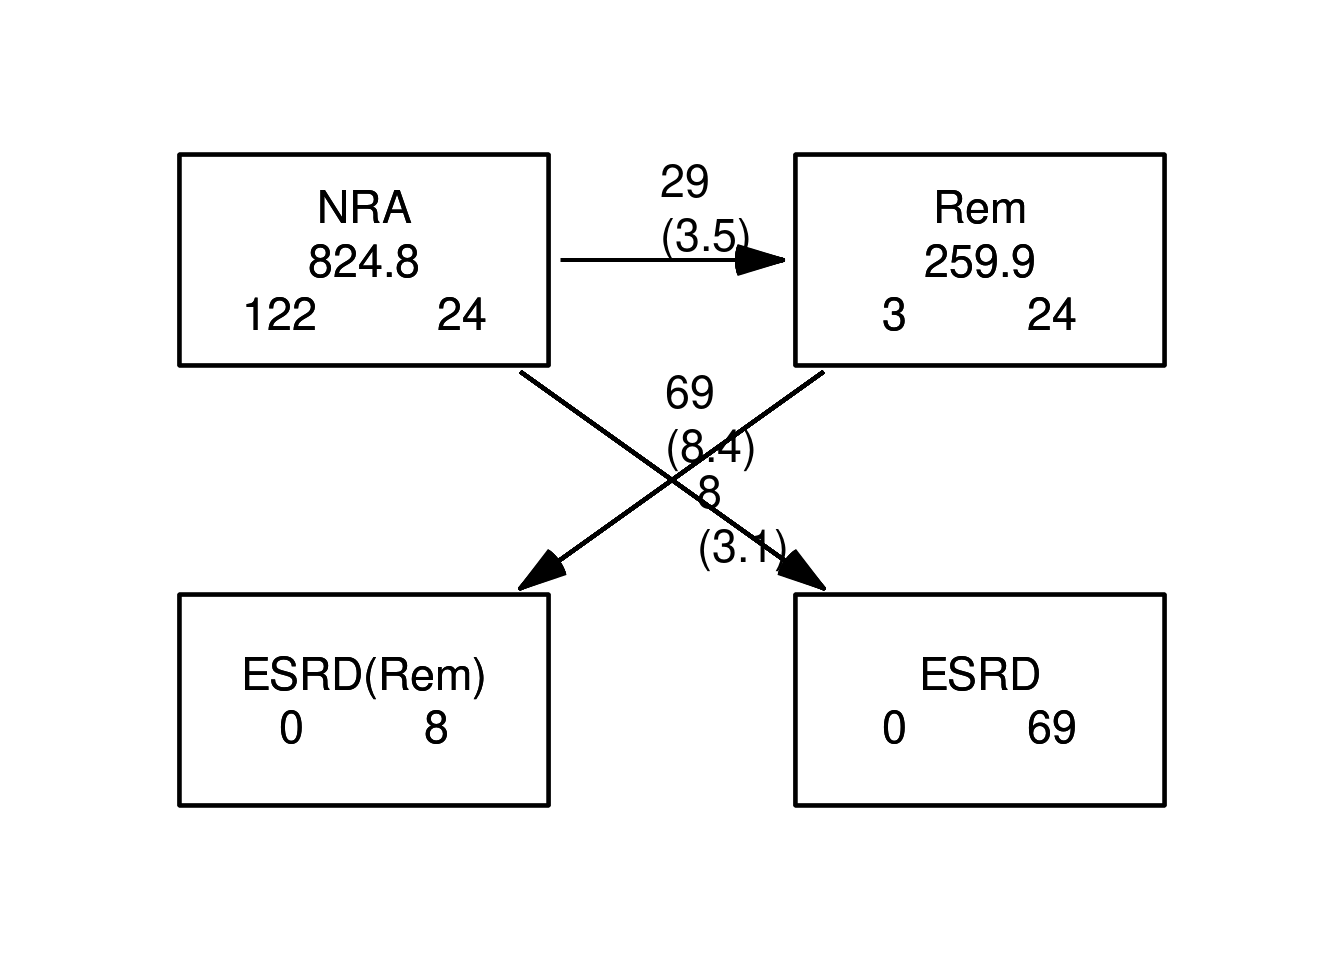
\includegraphics{renal-s_files/figure-latex/Lc-boxes-1.pdf}

  You may even be tempted to read the help page for
  \texttt{boxes.Lexis} \ldots{}
\item
  Plot a Lexis diagram where different coloring is
  used for different segments of the follow-up. The
  \texttt{plot.Lexis} function draws a line for each record in the
  dataset, so you can index the coloring by \texttt{lex.Cst} and
  \texttt{lex.Xst} as appropriate --- indexing by a factor corresponds
  to indexing by the \emph{index number} of the factor levels, so you
  must be know which order the factor levels are in:

\begin{Shaded}
\begin{Highlighting}[]
\FunctionTok{levels}\NormalTok{(Lc) }\CommentTok{\# names and order of states in lex.Cst and lex.Xst}
\end{Highlighting}
\end{Shaded}

\begin{verbatim}
[1] "NRA"       "Rem"       "ESRD"      "ESRD(Rem)"
\end{verbatim}

\begin{Shaded}
\begin{Highlighting}[]
\FunctionTok{par}\NormalTok{(}\AttributeTok{mai =} \FunctionTok{c}\NormalTok{(}\DecValTok{3}\NormalTok{, }\DecValTok{3}\NormalTok{, }\DecValTok{1}\NormalTok{, }\DecValTok{1}\NormalTok{) }\SpecialCharTok{/} \DecValTok{4}\NormalTok{, }\AttributeTok{mgp =} \FunctionTok{c}\NormalTok{(}\DecValTok{3}\NormalTok{, }\DecValTok{1}\NormalTok{, }\DecValTok{0}\NormalTok{) }\SpecialCharTok{/} \FloatTok{1.6}\NormalTok{)}
\FunctionTok{plot}\NormalTok{(Lc, }\AttributeTok{col =} \FunctionTok{c}\NormalTok{(}\StringTok{"red"}\NormalTok{, }\StringTok{"limegreen"}\NormalTok{)[Lc}\SpecialCharTok{$}\NormalTok{lex.Cst],}
        \AttributeTok{xlab =} \StringTok{"Calendar time"}\NormalTok{, }\AttributeTok{ylab =} \StringTok{"Age"}\NormalTok{,}
         \AttributeTok{lwd =} \DecValTok{3}\NormalTok{, }\AttributeTok{grid =} \DecValTok{0}\SpecialCharTok{:}\DecValTok{20} \SpecialCharTok{*} \DecValTok{5}\NormalTok{, }\AttributeTok{las =} \DecValTok{1}\NormalTok{,}
        \AttributeTok{xlim =} \FunctionTok{c}\NormalTok{(}\DecValTok{1970}\NormalTok{, }\DecValTok{2010}\NormalTok{), }\AttributeTok{ylim =} \FunctionTok{c}\NormalTok{(}\DecValTok{20}\NormalTok{, }\DecValTok{70}\NormalTok{), }
        \AttributeTok{xaxs =} \StringTok{"i"}\NormalTok{, }\AttributeTok{yaxs =} \StringTok{"i"}\NormalTok{)}
\FunctionTok{points}\NormalTok{(Lc, }\AttributeTok{pch =} \FunctionTok{c}\NormalTok{(}\ConstantTok{NA}\NormalTok{, }\ConstantTok{NA}\NormalTok{, }\DecValTok{16}\NormalTok{, }\DecValTok{16}\NormalTok{)[Lc}\SpecialCharTok{$}\NormalTok{lex.Xst],}
           \AttributeTok{col =} \FunctionTok{c}\NormalTok{(}\StringTok{"red"}\NormalTok{, }\StringTok{"limegreen"}\NormalTok{, }\StringTok{"transparent"}\NormalTok{, }\StringTok{"transparent"}\NormalTok{)[Lc}\SpecialCharTok{$}\NormalTok{lex.Cst])}
\FunctionTok{points}\NormalTok{(Lc, }\AttributeTok{pch =} \FunctionTok{c}\NormalTok{(}\ConstantTok{NA}\NormalTok{, }\ConstantTok{NA}\NormalTok{, }\DecValTok{1}\NormalTok{, }\DecValTok{1}\NormalTok{)[Lc}\SpecialCharTok{$}\NormalTok{lex.Xst],}
           \AttributeTok{col =} \StringTok{"black"}\NormalTok{, }\AttributeTok{lwd =} \DecValTok{2}\NormalTok{)}
\end{Highlighting}
\end{Shaded}

  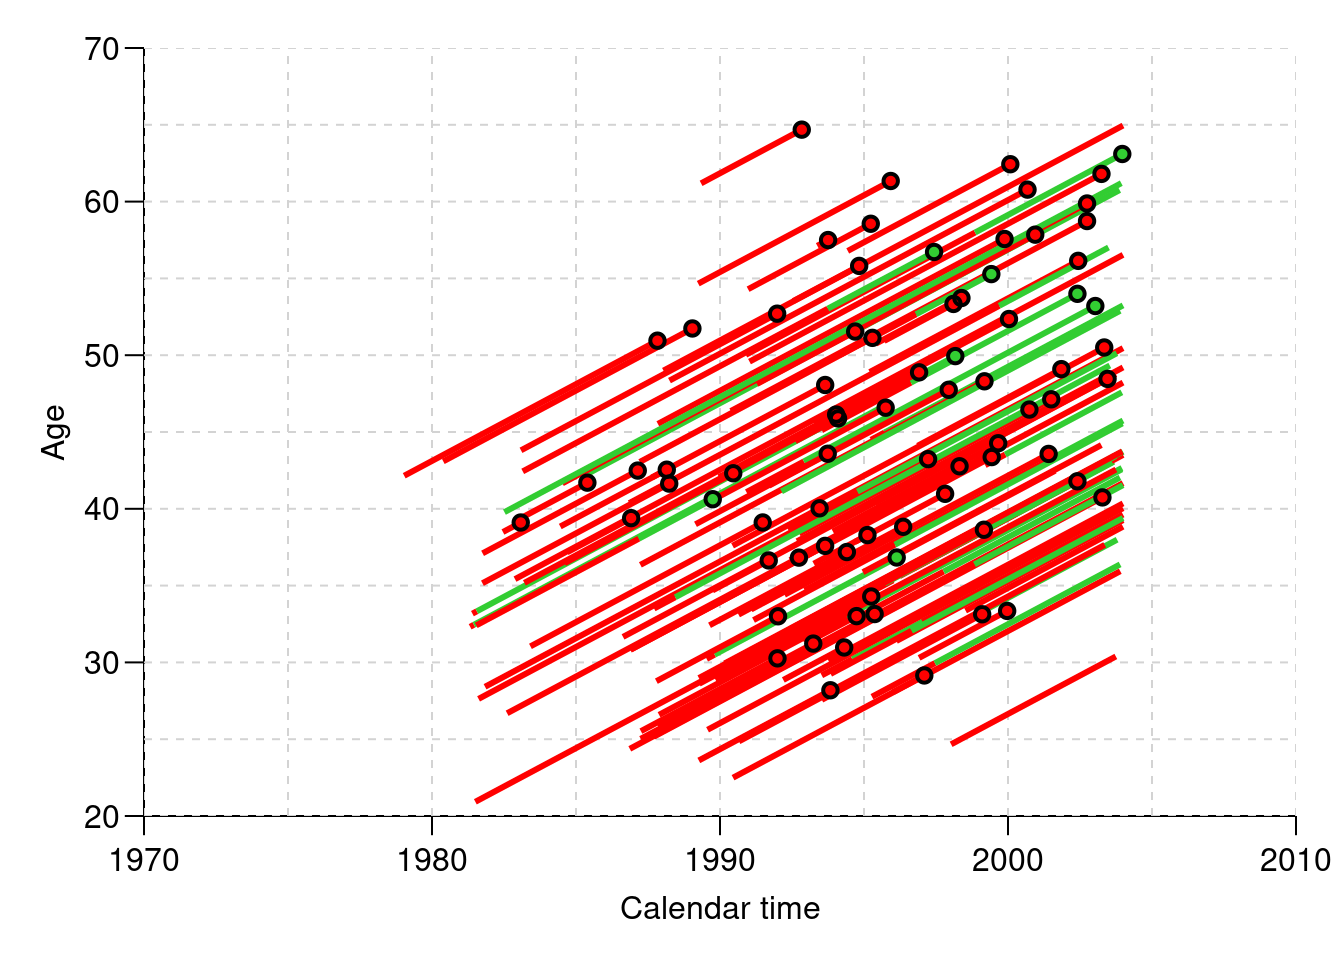
\includegraphics{renal-s_files/figure-latex/Lexis-rem-1.pdf}
\item
  Make a Cox-regression of mortality rates (i.e.~endpoint \texttt{ESRD} or
  \texttt{ESRD(Rem)}) with sex, age at entry and remission as
  explanatory variables, using time since entry as timescale, and
  include \texttt{lex.Cst} as time-dependent variable, and
  indicate that each record represents follow-up from
  \texttt{tfi} to \texttt{tfi+lex.dur}. Make sure that you know
  why what goes where here in the call to \texttt{coxph}.

\begin{Shaded}
\begin{Highlighting}[]
\NormalTok{(EP }\OtherTok{\textless{}{-}} \FunctionTok{levels}\NormalTok{(Lc)[}\DecValTok{3}\SpecialCharTok{:}\DecValTok{4}\NormalTok{])           }\CommentTok{\# define EndPoint states}
\end{Highlighting}
\end{Shaded}

\begin{verbatim}
[1] "ESRD"      "ESRD(Rem)"
\end{verbatim}

\begin{Shaded}
\begin{Highlighting}[]
\NormalTok{m1 }\OtherTok{\textless{}{-}} \FunctionTok{coxph}\NormalTok{(}\FunctionTok{Surv}\NormalTok{(tfi,             }\CommentTok{\# entry time}
\NormalTok{                 tfi }\SpecialCharTok{+}\NormalTok{ lex.dur,   }\CommentTok{\# exit time}
\NormalTok{                 lex.Xst }\SpecialCharTok{\%in\%}\NormalTok{ EP) }\CommentTok{\# event}
            \SpecialCharTok{\textasciitilde{}}\NormalTok{ sex }\SpecialCharTok{+} \FunctionTok{I}\NormalTok{((doe }\SpecialCharTok{{-}}\NormalTok{ dob }\SpecialCharTok{{-}} \DecValTok{50}\NormalTok{) }\SpecialCharTok{/} \DecValTok{10}\NormalTok{) }\SpecialCharTok{+} \CommentTok{\# fixed covariates}
\NormalTok{              (lex.Cst }\SpecialCharTok{==} \StringTok{"Rem"}\NormalTok{),              }\CommentTok{\# time{-}dependent variable}
            \AttributeTok{data =}\NormalTok{ Lc)}
\FunctionTok{summary}\NormalTok{(m1)}
\end{Highlighting}
\end{Shaded}

\begin{verbatim}
Call:
coxph(formula = Surv(tfi, tfi + lex.dur, lex.Xst %in% EP) ~ sex + 
    I((doe - dob - 50)/10) + (lex.Cst == "Rem"), data = Lc)

  n= 154, number of events= 77 

                           coef exp(coef) se(coef)      z Pr(>|z|)
sexF                   -0.05534   0.94616  0.27500 -0.201 0.840517
I((doe - dob - 50)/10)  0.52190   1.68522  0.13655  3.822 0.000132
lex.Cst == "Rem"TRUE   -1.26241   0.28297  0.38483 -3.280 0.001036

                       exp(coef) exp(-coef) lower .95 upper .95
sexF                      0.9462     1.0569    0.5519    1.6220
I((doe - dob - 50)/10)    1.6852     0.5934    1.2895    2.2024
lex.Cst == "Rem"TRUE      0.2830     3.5339    0.1331    0.6016

Concordance= 0.664  (se = 0.033 )
Likelihood ratio test= 30.31  on 3 df,   p=1e-06
Wald test            = 27.07  on 3 df,   p=6e-06
Score (logrank) test = 29.41  on 3 df,   p=2e-06
\end{verbatim}

  What is the effect of of remission on the rate of ESRD?

  \section{Splitting the follow-up time}\label{splitting-the-follow-up-time}

  In order to explore the effect of remission on the rate of ESRD, we
  split the data further into small pieces of follow-up. To this
  end we use the function \texttt{splitLexis}. The rates can then be
  modeled using a Poisson-model, and the shape of the effect of the
  underlying \emph{rates} be explored. Furthermore, we can allow effects of both
  time since NRA and current age. To this end we will use splines, so we
  need the \texttt{splines} and also the \texttt{mgcv} packages.
\item
  Now split the follow-up time every month after entry, and verify
  that the number of events and risk time is the same as before and
  after the split:

\begin{Shaded}
\begin{Highlighting}[]
\NormalTok{sLc }\OtherTok{\textless{}{-}} \FunctionTok{splitLexis}\NormalTok{(Lc, }\StringTok{"tfi"}\NormalTok{, }\AttributeTok{breaks =} \FunctionTok{seq}\NormalTok{(}\DecValTok{0}\NormalTok{, }\DecValTok{30}\NormalTok{, }\DecValTok{1}\SpecialCharTok{/}\DecValTok{12}\NormalTok{))}
\FunctionTok{summary}\NormalTok{( Lc)}
\end{Highlighting}
\end{Shaded}

\begin{verbatim}

Transitions:
     To
From  NRA Rem ESRD ESRD(Rem)  Records:  Events: Risk time:  Persons:
  NRA  24  29   69         0       122       98     824.77       122
  Rem   0  24    0         8        32        8     259.90        32
  Sum  24  53   69         8       154      106    1084.67       125
\end{verbatim}

\begin{Shaded}
\begin{Highlighting}[]
\FunctionTok{summary}\NormalTok{(sLc)}
\end{Highlighting}
\end{Shaded}

\begin{verbatim}

Transitions:
     To
From   NRA  Rem ESRD ESRD(Rem)  Records:  Events: Risk time:  Persons:
  NRA 9854   29   69         0      9952       98     824.77       122
  Rem    0 3139    0         8      3147        8     259.90        32
  Sum 9854 3168   69         8     13099      106    1084.67       125
\end{verbatim}
\item
  Now fit the Poisson-model corresponding to the Cox-model
  we fitted previously. The function \texttt{Ns()} produces a model
  matrix corresponding to a piece-wise cubic function, modeling the
  baseline hazard explicitly (think of the \texttt{Ns} terms as the
  baseline hazard that is not visible in the Cox-model). You
  can use the wrapper function \texttt{glm.Lexis}

\begin{Shaded}
\begin{Highlighting}[]
\NormalTok{mp }\OtherTok{\textless{}{-}} \FunctionTok{glm.Lexis}\NormalTok{(sLc, }
                \SpecialCharTok{\textasciitilde{}} \FunctionTok{Ns}\NormalTok{(tfi, }\AttributeTok{knots =} \FunctionTok{c}\NormalTok{(}\DecValTok{0}\NormalTok{, }\DecValTok{2}\NormalTok{, }\DecValTok{5}\NormalTok{, }\DecValTok{10}\NormalTok{)) }\SpecialCharTok{+}
\NormalTok{                  sex }\SpecialCharTok{+} \FunctionTok{I}\NormalTok{((doe }\SpecialCharTok{{-}}\NormalTok{ dob }\SpecialCharTok{{-}} \DecValTok{40}\NormalTok{) }\SpecialCharTok{/} \DecValTok{10}\NormalTok{) }\SpecialCharTok{+} 
                  \FunctionTok{I}\NormalTok{(lex.Cst }\SpecialCharTok{==} \StringTok{"Rem"}\NormalTok{))}
\end{Highlighting}
\end{Shaded}

\begin{verbatim}
stats::glm Poisson analysis of Lexis object sLc with log link:
Rates for transitions:
NRA->ESRD
Rem->ESRD(Rem)
\end{verbatim}

\begin{Shaded}
\begin{Highlighting}[]
\FunctionTok{ci.exp}\NormalTok{(mp)}
\end{Highlighting}
\end{Shaded}

\begin{verbatim}
                                   exp(Est.)        2.5%        97.5%
(Intercept)                       0.01664432 0.003956666   0.07001685
Ns(tfi, knots = c(0, 2, 5, 10))1  5.18917655 1.949197027  13.81469029
Ns(tfi, knots = c(0, 2, 5, 10))2 34.20004199 1.764818735 662.75524463
Ns(tfi, knots = c(0, 2, 5, 10))3  4.43318269 2.179977108   9.01528219
sexF                              0.91751162 0.536258443   1.56981691
I((doe - dob - 40)/10)            1.70082390 1.300813859   2.22384004
I(lex.Cst == "Rem")TRUE           0.27927558 0.131396852   0.59358233
\end{verbatim}

  How does the effects of sex change from the Cox-model?
\item
  Try instead using the \texttt{gam} function from the
  \texttt{mgcv} package. There is convenience wrapper for this for
  \texttt{Lexis} objects as well:

\begin{Shaded}
\begin{Highlighting}[]
\NormalTok{mx }\OtherTok{\textless{}{-}} \FunctionTok{gam.Lexis}\NormalTok{(sLc,}
                \SpecialCharTok{\textasciitilde{}} \FunctionTok{s}\NormalTok{(tfi, }\AttributeTok{k =} \DecValTok{10}\NormalTok{) }\SpecialCharTok{+} 
\NormalTok{                  sex }\SpecialCharTok{+} \FunctionTok{I}\NormalTok{((doe }\SpecialCharTok{{-}}\NormalTok{ dob }\SpecialCharTok{{-}} \DecValTok{40}\NormalTok{) }\SpecialCharTok{/} \DecValTok{10}\NormalTok{) }\SpecialCharTok{+} 
                  \FunctionTok{I}\NormalTok{(lex.Cst }\SpecialCharTok{==} \StringTok{"Rem"}\NormalTok{))}
\end{Highlighting}
\end{Shaded}

\begin{verbatim}
mgcv::gam Poisson analysis of Lexis object sLc with log link:
Rates for transitions:
NRA->ESRD
Rem->ESRD(Rem)
\end{verbatim}

\begin{Shaded}
\begin{Highlighting}[]
\FunctionTok{ci.exp}\NormalTok{(mp, }\AttributeTok{subset =} \FunctionTok{c}\NormalTok{(}\StringTok{"Cst"}\NormalTok{, }\StringTok{"doe"}\NormalTok{, }\StringTok{"sex"}\NormalTok{))}
\end{Highlighting}
\end{Shaded}

\begin{verbatim}
                        exp(Est.)      2.5%     97.5%
I(lex.Cst == "Rem")TRUE 0.2792756 0.1313969 0.5935823
I((doe - dob - 40)/10)  1.7008239 1.3008139 2.2238400
sexF                    0.9175116 0.5362584 1.5698169
\end{verbatim}

\begin{Shaded}
\begin{Highlighting}[]
\FunctionTok{ci.exp}\NormalTok{(mx, }\AttributeTok{subset =} \FunctionTok{c}\NormalTok{(}\StringTok{"Cst"}\NormalTok{, }\StringTok{"doe"}\NormalTok{, }\StringTok{"sex"}\NormalTok{))}
\end{Highlighting}
\end{Shaded}

\begin{verbatim}
                        exp(Est.)      2.5%     97.5%
I(lex.Cst == "Rem")TRUE 0.2784659 0.1309446 0.5921838
I((doe - dob - 40)/10)  1.6992069 1.2995225 2.2218192
sexF                    0.9309945 0.5435486 1.5946150
\end{verbatim}

  We see that there is virtually no difference between the two
  approaches in terms of the regression parameters.
\item
  Extract the regression parameters from the models using
  \texttt{ci.exp} and compare with the estimates from the Cox-model:

\begin{Shaded}
\begin{Highlighting}[]
\FunctionTok{ci.exp}\NormalTok{(mx, }\AttributeTok{subset =} \FunctionTok{c}\NormalTok{(}\StringTok{"sex"}\NormalTok{, }\StringTok{"dob"}\NormalTok{, }\StringTok{"Cst"}\NormalTok{), }\AttributeTok{pval =} \ConstantTok{TRUE}\NormalTok{)}
\end{Highlighting}
\end{Shaded}

\begin{verbatim}
                        exp(Est.)      2.5%     97.5%            P
sexF                    0.9309945 0.5435486 1.5946150 0.7945394004
I((doe - dob - 40)/10)  1.6992069 1.2995225 2.2218192 0.0001066910
I(lex.Cst == "Rem")TRUE 0.2784659 0.1309446 0.5921838 0.0008970863
\end{verbatim}

\begin{Shaded}
\begin{Highlighting}[]
\FunctionTok{ci.exp}\NormalTok{(m1)}
\end{Highlighting}
\end{Shaded}

\begin{verbatim}
                       exp(Est.)      2.5%    97.5%
sexF                   0.9461646 0.5519334 1.621985
I((doe - dob - 50)/10) 1.6852196 1.2895097 2.202360
lex.Cst == "Rem"TRUE   0.2829710 0.1330996 0.601599
\end{verbatim}

\begin{Shaded}
\begin{Highlighting}[]
\FunctionTok{round}\NormalTok{(}\FunctionTok{ci.exp}\NormalTok{(mp, }\AttributeTok{subset =} \FunctionTok{c}\NormalTok{(}\StringTok{"sex"}\NormalTok{, }\StringTok{"dob"}\NormalTok{, }\StringTok{"Cst"}\NormalTok{)) }\SpecialCharTok{/} \FunctionTok{ci.exp}\NormalTok{(m1), }\DecValTok{2}\NormalTok{)}
\end{Highlighting}
\end{Shaded}

\begin{verbatim}
                        exp(Est.) 2.5% 97.5%
sexF                         0.97 0.97  0.97
I((doe - dob - 40)/10)       1.01 1.01  1.01
I(lex.Cst == "Rem")TRUE      0.99 0.99  0.99
\end{verbatim}

  How large are the differences in estimated regression parameters?
\item
  The model has the same assumptions as the Cox-model about
  proportionality of rates, but there is an additional assumption that
  the hazard is a smooth function of time since entry. It seems to be
  a sensible assumption (well, restriction) to put on the rates that
  they vary smoothly by time. No such restriction is made in the Cox
  model. The \texttt{gam} model optimizes the shape of the smoother by
  general cross-validation. Try to look at the shape of the
  estimated effect of \texttt{tfi}:

\begin{Shaded}
\begin{Highlighting}[]
\FunctionTok{plot}\NormalTok{(mx)}
\end{Highlighting}
\end{Shaded}

  \includegraphics{renal-s_files/figure-latex/unnamed-chunk-13-1.pdf}

  Is this a useful plot?
\item
  However, \texttt{plot} (well, \texttt{plot.gam}) does not give you the \emph{absolute}
  level of the underlying rates because it bypasses the intercept. So
  in order to predict the rates as a function of \texttt{tfi} and the
  covariates, we set up a prediction data frame. Note that age
  in the model specification is entered as \texttt{doe-dob}, hence
  the prediction data frame must have these two variables and not
  the age, but it is only the difference that matters for the prediction:

\begin{Shaded}
\begin{Highlighting}[]
\NormalTok{nd }\OtherTok{\textless{}{-}} \FunctionTok{data.frame}\NormalTok{(}\AttributeTok{tfi =} \FunctionTok{seq}\NormalTok{(}\DecValTok{0}\NormalTok{, }\DecValTok{20}\NormalTok{, }\FloatTok{0.1}\NormalTok{),}
                 \AttributeTok{sex =} \StringTok{"M"}\NormalTok{,}
                 \AttributeTok{doe =} \DecValTok{1990}\NormalTok{,}
                 \AttributeTok{dob =} \DecValTok{1940}\NormalTok{,}
             \AttributeTok{lex.Cst =} \StringTok{"NRA"}\NormalTok{)}
\FunctionTok{str}\NormalTok{(nd)}
\end{Highlighting}
\end{Shaded}

\begin{verbatim}
'data.frame':   201 obs. of  5 variables:
 $ tfi    : num  0 0.1 0.2 0.3 0.4 0.5 0.6 0.7 0.8 0.9 ...
 $ sex    : chr  "M" "M" "M" "M" ...
 $ doe    : num  1990 1990 1990 1990 1990 1990 1990 1990 1990 1990 ...
 $ dob    : num  1940 1940 1940 1940 1940 1940 1940 1940 1940 1940 ...
 $ lex.Cst: chr  "NRA" "NRA" "NRA" "NRA" ...
\end{verbatim}

\begin{Shaded}
\begin{Highlighting}[]
\FunctionTok{matshade}\NormalTok{(nd}\SpecialCharTok{$}\NormalTok{tfi, }\FunctionTok{cbind}\NormalTok{(}\FunctionTok{ci.pred}\NormalTok{(mp, }\AttributeTok{newdata =}\NormalTok{ nd),}
                       \FunctionTok{ci.pred}\NormalTok{(mx, }\AttributeTok{newdata =}\NormalTok{ nd)) }\SpecialCharTok{*} \DecValTok{100}\NormalTok{,}
         \AttributeTok{plot =} \ConstantTok{TRUE}\NormalTok{,}
         \AttributeTok{type =} \StringTok{"l"}\NormalTok{, }\AttributeTok{lwd =} \DecValTok{3}\SpecialCharTok{:}\DecValTok{4}\NormalTok{, }\AttributeTok{col =} \FunctionTok{c}\NormalTok{(}\StringTok{"black"}\NormalTok{, }\StringTok{"forestgreen"}\NormalTok{),}
         \AttributeTok{log =} \StringTok{"y"}\NormalTok{, }\AttributeTok{xlab =} \StringTok{"Time since entry (years)"}\NormalTok{,}
         \AttributeTok{ylab =} \StringTok{"ESRD rate (per 100 PY) for 50 year old men"}\NormalTok{)}
\end{Highlighting}
\end{Shaded}

  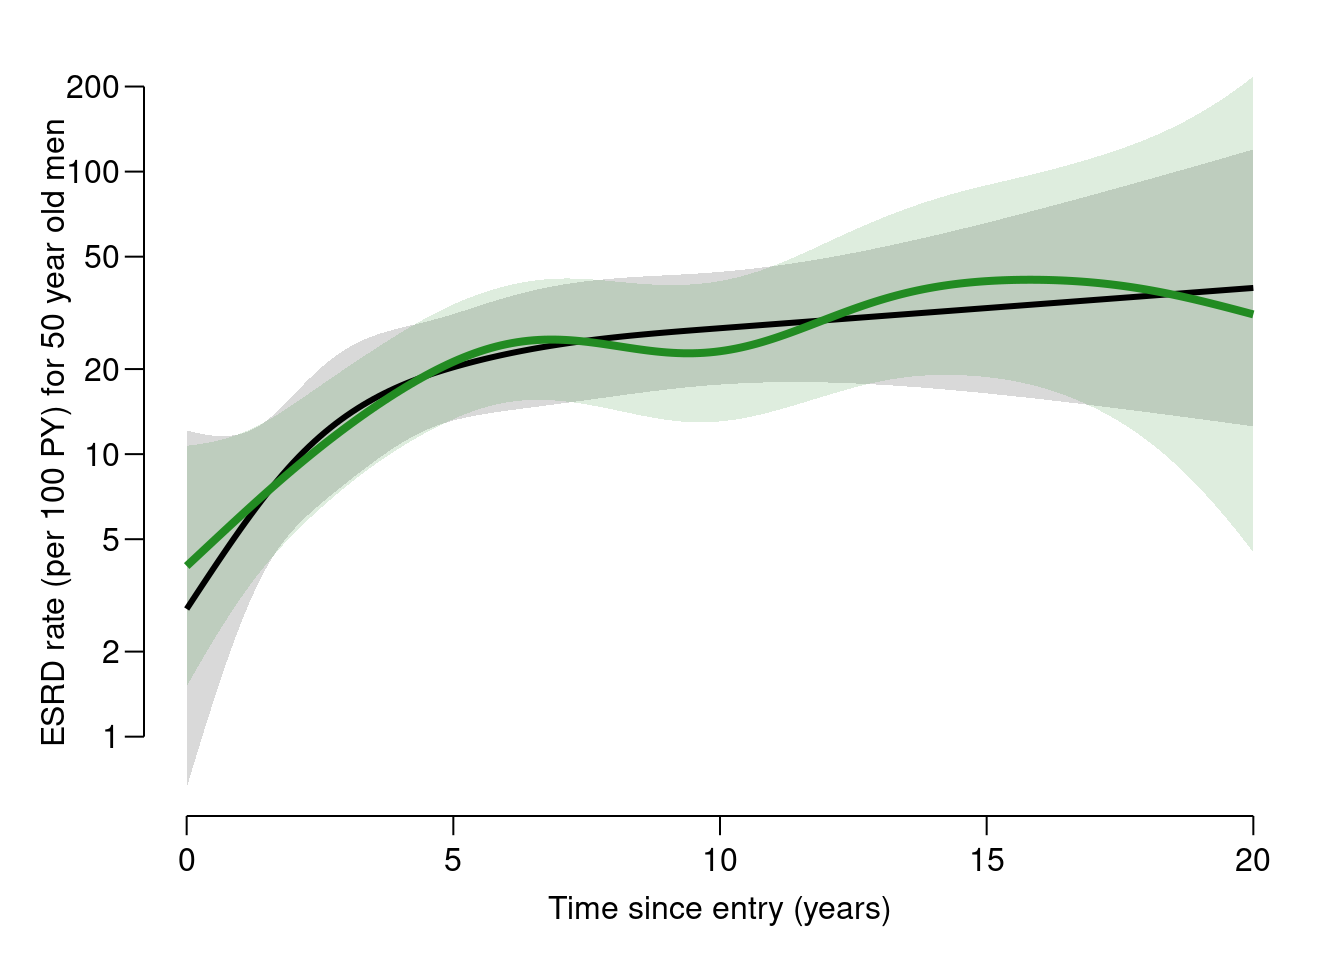
\includegraphics{renal-s_files/figure-latex/pred-1.pdf}
  Try to overlay with the corresponding prediction from the
  \texttt{glm} model using \texttt{Ns}.
\end{enumerate}

\#\# Prediction from the multistate model

\begin{verbatim}
If we want to make proper statements about the survival and disease
probabilities we must know not only how the occurrence of remission
influences the rate of death/ESRD, but we must also model the
occurrence rate of remission itself.
\end{verbatim}

\begin{enumerate}
\def\labelenumi{\arabic{enumi}.}
\setcounter{enumi}{16}
\item
  The rates of ESRD were modelled by a Poisson model with
  effects of age and time since NRA --- in the models \texttt{mp}
  and \texttt{mx}. But if we want to model whole process we must
  also model the remission rates transition from \texttt{NRA} to
  \texttt{Rem}, but the number of events is rather small so we restrict
  covariates in this model to only time since NRA and sex. Note
  that only the records that represent follow-up in the \texttt{NRA}
  state should be used; this is most easily done using the
  \texttt{gam.Lexis} function

\begin{Shaded}
\begin{Highlighting}[]
\NormalTok{mr }\OtherTok{\textless{}{-}} \FunctionTok{gam.Lexis}\NormalTok{(sLc, }\SpecialCharTok{\textasciitilde{}} \FunctionTok{s}\NormalTok{(tfi, }\AttributeTok{k =} \DecValTok{10}\NormalTok{) }\SpecialCharTok{+}\NormalTok{ sex,}
                     \AttributeTok{from =} \StringTok{"NRA"}\NormalTok{,}
                       \AttributeTok{to =} \StringTok{"Rem"}\NormalTok{)}
\end{Highlighting}
\end{Shaded}

\begin{verbatim}
mgcv::gam Poisson analysis of Lexis object sLc with log link:
Rates for the transition:
NRA->Rem
\end{verbatim}

\begin{Shaded}
\begin{Highlighting}[]
\FunctionTok{summary}\NormalTok{(mr)}
\end{Highlighting}
\end{Shaded}

\begin{verbatim}

Family: poisson 
Link function: log 

Formula:
cbind(trt(Lx$lex.Cst, Lx$lex.Xst) %in% trnam, Lx$lex.dur) ~ s(tfi, 
    k = 10) + sex

Parametric coefficients:
            Estimate Std. Error z value Pr(>|z|)
(Intercept)  -3.7025     0.2582 -14.339   <2e-16
sexF          0.9579     0.3728   2.569   0.0102

Approximate significance of smooth terms:
         edf Ref.df Chi.sq p-value
s(tfi) 1.013  1.025  0.066   0.813

R-sq.(adj) =  -5.65e-06   Deviance explained = 1.65%
UBRE = -0.96024  Scale est. = 1         n = 9952
\end{verbatim}

\begin{Shaded}
\begin{Highlighting}[]
\FunctionTok{ci.exp}\NormalTok{(mr, }\AttributeTok{pval =} \ConstantTok{TRUE}\NormalTok{)}
\end{Highlighting}
\end{Shaded}

\begin{verbatim}
             exp(Est.)       2.5%      97.5%            P
(Intercept) 0.02466174 0.01486718 0.04090901 1.254019e-46
sexF        2.60620470 1.25503844 5.41202779 1.019130e-02
s(tfi).1    1.00499489 0.89131271 1.13317662 9.351638e-01
s(tfi).2    0.99623769 0.80778743 1.22865188 9.718940e-01
s(tfi).3    0.99822247 0.91911268 1.08414140 9.663137e-01
s(tfi).4    1.00188999 0.89006998 1.12775801 9.750528e-01
s(tfi).5    0.99842904 0.92280785 1.08024715 9.687920e-01
s(tfi).6    0.99817367 0.90142303 1.10530865 9.719666e-01
s(tfi).7    1.00168704 0.92615949 1.08337380 9.663850e-01
s(tfi).8    0.99448155 0.68445450 1.44493689 9.768400e-01
s(tfi).9    0.94790052 0.63349476 1.41834700 7.946918e-01
\end{verbatim}

  What is the remission rate-ratio between men and women?
\item
  If we want to predict the probability of being in each of the
  three states using these estimated rates, we may resort to
  analytical calculations of the probabilities from the estimated
  rates, which is actually doable in this case, but which will be largely
  intractable for more complicated models.
  Alternatively we can \emph{simulate} the life course for a large
  group of (identical) individuals through a model using the estimated
  rates. That will give a simulated cohort (in the form of a
  \texttt{Lexis} object), and we can then just count the number of
  persons in each state at each of a set of time points.
  This is accomplished using the function \texttt{simLexis}. The input
  to this is the initial status of the persons whose life-course we
  shall simulate, and the transition rates in suitable form:

  \begin{itemize}
  \tightlist
  \item
    Suppose we want predictions for men aged 50 at
    NRA. The input is in the form of a \texttt{Lexis} object (where
    \texttt{lex.dur} and \texttt{lex.Xst} will be ignored). Note that in
    order to carry over the \texttt{time.scales} and the
    \texttt{time.since} attributes, we construct the input object using
    \texttt{subset} to select columns, and \texttt{NULL} to select rows
    (see the example in the help file for \texttt{simLexis}):
  \end{itemize}

\begin{Shaded}
\begin{Highlighting}[]
\NormalTok{inL }\OtherTok{\textless{}{-}} \FunctionTok{subset}\NormalTok{(sLc, }\AttributeTok{select =} \DecValTok{1}\SpecialCharTok{:}\DecValTok{11}\NormalTok{)[}\ConstantTok{NULL}\NormalTok{, ]}
\FunctionTok{str}\NormalTok{(inL)}
\end{Highlighting}
\end{Shaded}

\begin{verbatim}
Classes 'Lexis' and 'data.frame':   0 obs. of  11 variables:
 $ lex.id : int 
 $ per    : num 
 $ age    : num 
 $ tfi    : num 
 $ lex.dur: num 
 $ lex.Cst: Factor w/ 4 levels "NRA","Rem","ESRD",..: 
 $ lex.Xst: Factor w/ 4 levels "NRA","Rem","ESRD",..: 
 $ id     : num 
 $ sex    : Factor w/ 2 levels "M","F": 
 $ dob    : num 
 $ doe    : num 
 - attr(*, "time.scales")= chr [1:3] "per" "age" "tfi"
 - attr(*, "time.since")= chr [1:3] "" "" ""
 - attr(*, "breaks")=List of 3
  ..$ per: NULL
  ..$ age: NULL
  ..$ tfi: num [1:361] 0 0.0833 0.1667 0.25 0.3333 ...
\end{verbatim}

\begin{Shaded}
\begin{Highlighting}[]
\FunctionTok{timeScales}\NormalTok{(inL)}
\end{Highlighting}
\end{Shaded}

\begin{verbatim}
[1] "per" "age" "tfi"
\end{verbatim}

\begin{Shaded}
\begin{Highlighting}[]
\NormalTok{inL[}\DecValTok{1}\NormalTok{, }\StringTok{"lex.id"}\NormalTok{] }\OtherTok{\textless{}{-}} \DecValTok{1}
\NormalTok{inL[}\DecValTok{1}\NormalTok{, }\StringTok{"per"}\NormalTok{] }\OtherTok{\textless{}{-}} \DecValTok{2000}
\NormalTok{inL[}\DecValTok{1}\NormalTok{, }\StringTok{"age"}\NormalTok{] }\OtherTok{\textless{}{-}} \DecValTok{50}
\NormalTok{inL[}\DecValTok{1}\NormalTok{, }\StringTok{"tfi"}\NormalTok{] }\OtherTok{\textless{}{-}} \DecValTok{0}
\NormalTok{inL[}\DecValTok{1}\NormalTok{, }\StringTok{"lex.Cst"}\NormalTok{] }\OtherTok{\textless{}{-}} \StringTok{"NRA"}
\NormalTok{inL[}\DecValTok{1}\NormalTok{, }\StringTok{"lex.Xst"}\NormalTok{] }\OtherTok{\textless{}{-}} \ConstantTok{NA}
\NormalTok{inL[}\DecValTok{1}\NormalTok{, }\StringTok{"lex.dur"}\NormalTok{] }\OtherTok{\textless{}{-}} \ConstantTok{NA}
\NormalTok{inL[}\DecValTok{1}\NormalTok{, }\StringTok{"sex"}\NormalTok{] }\OtherTok{\textless{}{-}} \StringTok{"M"}
\NormalTok{inL[}\DecValTok{1}\NormalTok{, }\StringTok{"doe"}\NormalTok{] }\OtherTok{\textless{}{-}} \DecValTok{2000}
\NormalTok{inL[}\DecValTok{1}\NormalTok{, }\StringTok{"dob"}\NormalTok{] }\OtherTok{\textless{}{-}} \DecValTok{1950}
\NormalTok{inL }\OtherTok{\textless{}{-}} \FunctionTok{rbind}\NormalTok{(inL, inL)}
\NormalTok{inL[}\DecValTok{2}\NormalTok{, }\StringTok{"sex"}\NormalTok{] }\OtherTok{\textless{}{-}} \StringTok{"F"}
\NormalTok{inL}
\end{Highlighting}
\end{Shaded}

\begin{verbatim}
 lex.id  per age tfi lex.dur lex.Cst lex.Xst id sex  dob  doe
      1 2000  50   0      NA     NRA    <NA> NA   M 1950 2000
      1 2000  50   0      NA     NRA    <NA> NA   F 1950 2000
\end{verbatim}

\begin{Shaded}
\begin{Highlighting}[]
\FunctionTok{str}\NormalTok{(inL)}
\end{Highlighting}
\end{Shaded}

\begin{verbatim}
Classes 'Lexis' and 'data.frame':   2 obs. of  11 variables:
 $ lex.id : num  1 1
 $ per    : num  2000 2000
 $ age    : num  50 50
 $ tfi    : num  0 0
 $ lex.dur: num  NA NA
 $ lex.Cst: Factor w/ 4 levels "NRA","Rem","ESRD",..: 1 1
 $ lex.Xst: Factor w/ 4 levels "NRA","Rem","ESRD",..: NA NA
 $ id     : num  NA NA
 $ sex    : Factor w/ 2 levels "M","F": 1 2
 $ dob    : num  1950 1950
 $ doe    : num  2000 2000
 - attr(*, "breaks")=List of 3
  ..$ per: NULL
  ..$ age: NULL
  ..$ tfi: num [1:361] 0 0.0833 0.1667 0.25 0.3333 ...
 - attr(*, "time.scales")= chr [1:3] "per" "age" "tfi"
 - attr(*, "time.since")= chr [1:3] "" "" ""
\end{verbatim}

  The other input for the simulation is the models for the transitions. This is given as
  a list with an element for each transient state (that is \texttt{NRA} and
  \texttt{Rem}), each of which is again a list with names equal to the
  states that can be reached from the transient state. The content of
  the list will be \texttt{glm} objects, in this case the models we
  just fitted, describing the transition rates:

\begin{Shaded}
\begin{Highlighting}[]
\NormalTok{Tr }\OtherTok{\textless{}{-}} \FunctionTok{list}\NormalTok{(}\StringTok{"NRA"} \OtherTok{=} \FunctionTok{list}\NormalTok{(}\StringTok{"Rem"}  \OtherTok{=}\NormalTok{ mr,}
                        \StringTok{"ESRD"} \OtherTok{=}\NormalTok{ mx),}
           \StringTok{"Rem"} \OtherTok{=} \FunctionTok{list}\NormalTok{(}\StringTok{"ESRD(Rem)"} \OtherTok{=}\NormalTok{ mx))}
\end{Highlighting}
\end{Shaded}

  With this as input we can now generate a cohort, using \texttt{N=5}
  to simulate life course of 10 persons (5 for each set of starting values
  in \texttt{inL}):

\begin{Shaded}
\begin{Highlighting}[]
\NormalTok{(iL }\OtherTok{\textless{}{-}} \FunctionTok{simLexis}\NormalTok{(Tr, inL, }\AttributeTok{N =} \DecValTok{10}\NormalTok{))}
\end{Highlighting}
\end{Shaded}

\begin{verbatim}
 lex.id     per   age  tfi lex.dur lex.Cst   lex.Xst id sex  dob  doe cens
      1 2000.00 50.00 0.00    2.16     NRA       Rem NA   M 1950 2000 2020
      1 2002.16 52.16 2.16    2.14     Rem ESRD(Rem) NA   M 1950 2000 2020
      2 2000.00 50.00 0.00    4.72     NRA       Rem NA   M 1950 2000 2020
      2 2004.72 54.72 4.72   15.07     Rem ESRD(Rem) NA   M 1950 2000 2020
      3 2000.00 50.00 0.00    4.74     NRA      ESRD NA   M 1950 2000 2020
      4 2000.00 50.00 0.00    5.16     NRA      ESRD NA   M 1950 2000 2020
      5 2000.00 50.00 0.00    7.38     NRA      ESRD NA   M 1950 2000 2020
      6 2000.00 50.00 0.00    3.25     NRA      ESRD NA   M 1950 2000 2020
      7 2000.00 50.00 0.00    1.43     NRA      ESRD NA   M 1950 2000 2020
      8 2000.00 50.00 0.00    3.93     NRA      ESRD NA   M 1950 2000 2020
      9 2000.00 50.00 0.00   11.28     NRA      ESRD NA   M 1950 2000 2020
     10 2000.00 50.00 0.00    9.41     NRA      ESRD NA   M 1950 2000 2020
     11 2000.00 50.00 0.00    6.53     NRA      ESRD NA   F 1950 2000 2020
     12 2000.00 50.00 0.00    2.80     NRA      ESRD NA   F 1950 2000 2020
     13 2000.00 50.00 0.00    7.89     NRA      ESRD NA   F 1950 2000 2020
     14 2000.00 50.00 0.00    6.70     NRA      ESRD NA   F 1950 2000 2020
     15 2000.00 50.00 0.00    4.72     NRA      ESRD NA   F 1950 2000 2020
     16 2000.00 50.00 0.00    1.20     NRA      ESRD NA   F 1950 2000 2020
     17 2000.00 50.00 0.00   10.50     NRA      ESRD NA   F 1950 2000 2020
     18 2000.00 50.00 0.00    9.75     NRA      ESRD NA   F 1950 2000 2020
     19 2000.00 50.00 0.00    3.77     NRA      ESRD NA   F 1950 2000 2020
     20 2000.00 50.00 0.00   12.06     NRA      ESRD NA   F 1950 2000 2020
\end{verbatim}

\begin{Shaded}
\begin{Highlighting}[]
\FunctionTok{summary}\NormalTok{(iL, }\AttributeTok{by =} \StringTok{"sex"}\NormalTok{)}
\end{Highlighting}
\end{Shaded}

\begin{verbatim}
$M

Transitions:
     To
From  NRA Rem ESRD ESRD(Rem)  Records:  Events: Risk time:  Persons:
  NRA   0   2    8         0        10       10      53.46        10
  Rem   0   0    0         2         2        2      17.21         2
  Sum   0   2    8         2        12       12      70.67        10

$F

Transitions:
     To
From  NRA Rem ESRD ESRD(Rem)  Records:  Events: Risk time:  Persons:
  NRA   0   0   10         0        10       10      65.91        10
\end{verbatim}

  What type of object have you got as \texttt{iL}?
\item
  Now generate the life course of, say, 5,000 persons, and look at the summary.
  The \texttt{system.time} command is just to tell you how long it
  took, you may want to start with 500 just to see how long that takes.

\begin{Shaded}
\begin{Highlighting}[]
\FunctionTok{system.time}\NormalTok{(sM }\OtherTok{\textless{}{-}} \FunctionTok{simLexis}\NormalTok{(Tr, inL, }\AttributeTok{N =} \DecValTok{500}\NormalTok{, }\AttributeTok{t.range =} \DecValTok{12}\NormalTok{))}
\end{Highlighting}
\end{Shaded}

\begin{verbatim}
   user  system elapsed 
  2.691   3.250   2.060 
\end{verbatim}

\begin{Shaded}
\begin{Highlighting}[]
\FunctionTok{summary}\NormalTok{(sM, }\AttributeTok{by =} \StringTok{"sex"}\NormalTok{)}
\end{Highlighting}
\end{Shaded}

\begin{verbatim}
$M

Transitions:
     To
From  NRA Rem ESRD ESRD(Rem)  Records:  Events: Risk time:  Persons:
  NRA  34  81  385         0       500      466    2685.72       500
  Rem   0  44    0        37        81       37     523.68        81
  Sum  34 125  385        37       581      503    3209.41       500

$F

Transitions:
     To
From  NRA Rem ESRD ESRD(Rem)  Records:  Events: Risk time:  Persons:
  NRA  22 163  315         0       500      478    2358.86       500
  Rem   0 108    0        55       163       55    1133.09       163
  Sum  22 271  315        55       663      533    3491.96       500
\end{verbatim}

  Why are there so many ESRD-events in the resulting data set?
\item
  Now count how many persons are present in each state
  at each time for the first 10 years after entry (which is at age 50). This
  can be done by using \texttt{nState}. Try:

\begin{Shaded}
\begin{Highlighting}[]
\NormalTok{nStm }\OtherTok{\textless{}{-}} \FunctionTok{nState}\NormalTok{(}\FunctionTok{subset}\NormalTok{(sM, sex }\SpecialCharTok{==} \StringTok{"M"}\NormalTok{), }\AttributeTok{time.scale =} \StringTok{"age"}\NormalTok{, }
               \AttributeTok{at =} \FunctionTok{seq}\NormalTok{(}\DecValTok{0}\NormalTok{, }\DecValTok{10}\NormalTok{, }\FloatTok{0.1}\NormalTok{), }
             \AttributeTok{from =} \DecValTok{50}\NormalTok{)}
\NormalTok{nStf }\OtherTok{\textless{}{-}} \FunctionTok{nState}\NormalTok{(}\FunctionTok{subset}\NormalTok{(sM, sex }\SpecialCharTok{==} \StringTok{"F"}\NormalTok{), }\AttributeTok{time.scale =} \StringTok{"age"}\NormalTok{, }
               \AttributeTok{at =} \FunctionTok{seq}\NormalTok{(}\DecValTok{0}\NormalTok{, }\DecValTok{10}\NormalTok{, }\FloatTok{0.1}\NormalTok{), }
             \AttributeTok{from =} \DecValTok{50}\NormalTok{)}
\FunctionTok{head}\NormalTok{(nStf, }\DecValTok{15}\NormalTok{)}
\end{Highlighting}
\end{Shaded}

\begin{verbatim}
      State
when   NRA Rem ESRD ESRD(Rem)
  50   500   0    0         0
  50.1 493   3    4         0
  50.2 486   5    9         0
  50.3 482   8   10         0
  50.4 476  12   12         0
  50.5 470  15   15         0
  50.6 464  19   17         0
  50.7 460  21   18         1
  50.8 455  25   19         1
  50.9 450  29   20         1
  51   443  32   24         1
  51.1 440  35   24         1
  51.2 432  39   27         2
  51.3 424  41   33         2
  51.4 410  49   39         2
\end{verbatim}

  What is in the object \texttt{nStf}?
\item
  With the counts of persons in each state at the
  designated time points (in \texttt{nStm}), compute the cumulative
  fraction over the states, arranged in order given by \texttt{perm}:

\begin{Shaded}
\begin{Highlighting}[]
\NormalTok{ppm }\OtherTok{\textless{}{-}} \FunctionTok{pState}\NormalTok{(nStm, }\AttributeTok{perm =} \FunctionTok{c}\NormalTok{(}\DecValTok{2}\NormalTok{, }\DecValTok{1}\NormalTok{, }\DecValTok{3}\NormalTok{, }\DecValTok{4}\NormalTok{))}
\NormalTok{ppf }\OtherTok{\textless{}{-}} \FunctionTok{pState}\NormalTok{(nStf, }\AttributeTok{perm =} \FunctionTok{c}\NormalTok{(}\DecValTok{2}\NormalTok{, }\DecValTok{1}\NormalTok{, }\DecValTok{3}\NormalTok{, }\DecValTok{4}\NormalTok{))}
\FunctionTok{head}\NormalTok{(ppf)}
\end{Highlighting}
\end{Shaded}

\begin{verbatim}
      State
when     Rem   NRA ESRD ESRD(Rem)
  50   0.000 1.000    1         1
  50.1 0.006 0.992    1         1
  50.2 0.010 0.982    1         1
  50.3 0.016 0.980    1         1
  50.4 0.024 0.976    1         1
  50.5 0.030 0.970    1         1
\end{verbatim}

\begin{Shaded}
\begin{Highlighting}[]
\FunctionTok{tail}\NormalTok{(ppf)}
\end{Highlighting}
\end{Shaded}

\begin{verbatim}
      State
when     Rem   NRA  ESRD ESRD(Rem)
  59.5 0.230 0.338 0.918         1
  59.6 0.232 0.336 0.918         1
  59.7 0.232 0.336 0.918         1
  59.8 0.232 0.332 0.918         1
  59.9 0.232 0.332 0.918         1
  60   0.232 0.332 0.918         1
\end{verbatim}

  What do the entries in \texttt{ppf} represent?
\item
  Try to plot the cumulative probabilities using the \texttt{plot} method
  for \texttt{pState} objects:

\begin{Shaded}
\begin{Highlighting}[]
\FunctionTok{plot}\NormalTok{(ppf)}
\end{Highlighting}
\end{Shaded}

  \includegraphics{renal-s_files/figure-latex/plot-pp-1.pdf}

  Is this useful?
\item
  Now try to improve the plot so that it is easier to read, and
  easier to compare between men and women, for example:

\begin{Shaded}
\begin{Highlighting}[]
\FunctionTok{par}\NormalTok{(}\AttributeTok{mfrow =} \FunctionTok{c}\NormalTok{(}\DecValTok{1}\NormalTok{, }\DecValTok{2}\NormalTok{))}
\CommentTok{\# Men}
\FunctionTok{plot}\NormalTok{(ppm, }\AttributeTok{col =} \FunctionTok{c}\NormalTok{(}\StringTok{"limegreen"}\NormalTok{, }\StringTok{"red"}\NormalTok{, }\StringTok{"\#991111"}\NormalTok{, }\StringTok{"forestgreen"}\NormalTok{))}
\FunctionTok{lines}\NormalTok{(}\FunctionTok{as.numeric}\NormalTok{(}\FunctionTok{rownames}\NormalTok{(ppm)), ppm[, }\StringTok{"NRA"}\NormalTok{], }\AttributeTok{lwd =} \DecValTok{2}\NormalTok{)}
\FunctionTok{text}\NormalTok{(}\FloatTok{59.5}\NormalTok{, }\FloatTok{0.95}\NormalTok{, }\StringTok{"Men"}\NormalTok{, }\AttributeTok{adj =} \DecValTok{1}\NormalTok{, }\AttributeTok{col =} \StringTok{"white"}\NormalTok{, }\AttributeTok{font =} \DecValTok{2}\NormalTok{, }\AttributeTok{cex =} \FloatTok{1.2}\NormalTok{)}
\FunctionTok{axis}\NormalTok{(}\AttributeTok{side =} \DecValTok{4}\NormalTok{, }\AttributeTok{at =} \DecValTok{0}\SpecialCharTok{:}\DecValTok{10} \SpecialCharTok{/} \DecValTok{10}\NormalTok{)}
\FunctionTok{axis}\NormalTok{(}\AttributeTok{side =} \DecValTok{4}\NormalTok{, }\AttributeTok{at =} \DecValTok{1}\SpecialCharTok{:}\DecValTok{99} \SpecialCharTok{/} \DecValTok{100}\NormalTok{, }\AttributeTok{labels =} \ConstantTok{NA}\NormalTok{, }\AttributeTok{tck =} \SpecialCharTok{{-}}\FloatTok{0.01}\NormalTok{)}
\CommentTok{\# Women }
\FunctionTok{plot}\NormalTok{(ppf, }\AttributeTok{col =} \FunctionTok{c}\NormalTok{(}\StringTok{"limegreen"}\NormalTok{, }\StringTok{"red"}\NormalTok{, }\StringTok{"\#991111"}\NormalTok{, }\StringTok{"forestgreen"}\NormalTok{),}
          \AttributeTok{xlim =} \FunctionTok{c}\NormalTok{(}\DecValTok{60}\NormalTok{, }\DecValTok{50}\NormalTok{)) }\CommentTok{\# inverted x{-}axis}
\FunctionTok{lines}\NormalTok{(}\FunctionTok{as.numeric}\NormalTok{(}\FunctionTok{rownames}\NormalTok{(ppf)), ppf[, }\StringTok{"NRA"}\NormalTok{], }\AttributeTok{lwd =} \DecValTok{2}\NormalTok{)}
\FunctionTok{text}\NormalTok{(}\FloatTok{59.5}\NormalTok{, }\FloatTok{0.95}\NormalTok{, }\StringTok{"Women"}\NormalTok{, }\AttributeTok{adj =} \DecValTok{0}\NormalTok{, }\AttributeTok{col =} \StringTok{"white"}\NormalTok{, }\AttributeTok{font =} \DecValTok{2}\NormalTok{, }\AttributeTok{cex =} \FloatTok{1.2}\NormalTok{)}
\FunctionTok{axis}\NormalTok{(}\AttributeTok{side =} \DecValTok{2}\NormalTok{, }\AttributeTok{at =} \DecValTok{0}\SpecialCharTok{:}\DecValTok{10} \SpecialCharTok{/} \DecValTok{10}\NormalTok{)}
\FunctionTok{axis}\NormalTok{(}\AttributeTok{side =} \DecValTok{2}\NormalTok{, }\AttributeTok{at =} \DecValTok{1}\SpecialCharTok{:}\DecValTok{99} \SpecialCharTok{/} \DecValTok{100}\NormalTok{, }\AttributeTok{labels =} \ConstantTok{NA}\NormalTok{, }\AttributeTok{tck =} \SpecialCharTok{{-}}\FloatTok{0.01}\NormalTok{)}
\end{Highlighting}
\end{Shaded}

  \includegraphics{renal-s_files/figure-latex/new-nState-1.pdf}

  What is the 10-year risk of remission for men and women respectively?
\end{enumerate}

  \bibliography{book.bib,packages.bib}

\end{document}
